\documentclass[upright, contnum]{umemoria}
\depto{DEPARTAMENTO DE CIENCIAS DE LA COMPUTACIÓN}
\author{Manuel Osvaldo J. Olguín Muñoz}
\title{Diseño e Implementación de un Framework Integrado para Simulaciones de Sistemas Inteligentes de Transporte en OMNeT++ y Paramics}
\auspicio{NIC Chile Research Labs}
\date{Julio 2017}
\guia{Sandra Céspedes U.}
\carrera{INGENIERO CIVIL EN COMPUTACIÓN}
\memoria{MEMORIA PARA OPTAR AL TÍTULO DE INGENIERO CIVIL EN COMPUTACIÓN}
\comision{Javier Bustos, Nancy Hitschfeld}

\usepackage{lipsum}
\usepackage{multicol}
\usepackage[]{inputenc}
\usepackage[T1]{fontenc}
\usepackage{bytefield}
\usepackage{subcaption}
\usepackage{pgf-umlsd}
\usepackage{pgf-umlcd}
\usepackage[spanish]{babel}
\usepackage[style=ieee, sorting=none]{biblatex}
\usepackage{csquotes}
\usepackage{appendix}
\usepackage{listings}
\usepackage{float}
\usepackage{sourcecodepro}
\usepackage{tikz}
\usepackage{tikz-qtree}
\usepackage{dirtree}
\usepackage[labelfont=bf]{caption}
\usepackage{enumitem}
\usepackage{hyperref}
\setlist{  
    listparindent=\parindent
}

% reference description items
\makeatletter
\def\namedlabel#1#2{\begingroup
    #2%
    \def\@currentlabel{#2}%
    \phantomsection\label{#1}\endgroup
}
\makeatother

\captionsetup{format=hang}

% CPP style definition: %
\renewcommand{\lstlistingname}{Código}% Listing -> Código
\renewcommand{\lstlistlistingname}{Lista de \lstlistingname s}% List of Listings -> List of Algorithms
\definecolor{dkgreen}{rgb}{0,0.6,0}
\definecolor{gray}{rgb}{0.5,0.5,0.5}
\definecolor{lightgray}{rgb}{0.95, 0.95, 0.95}
\definecolor{mauve}{rgb}{0.58,0,0.82}
\definecolor{mygreen}{rgb}{0,0.6,0}
\definecolor{mygray}{rgb}{0.5,0.5,0.5}
\definecolor{mymauve}{rgb}{0.58,0,0.82}
\lstdefinestyle{CPP}{ % Estilo de lenguaje C++11
    language=[11]C++,
    frame=Lb,
    xleftmargin=\parindent,
    captionpos=b,
    aboveskip=3mm,
    belowskip=3mm,
    showstringspaces=false,
    columns=flexible,
    basicstyle={\small\ttfamily},
    numbers=left,
    numberstyle=\tiny\color{gray},
    keywordstyle=\color{purple},
    commentstyle=\color{gray},
    stringstyle=\color{dkgreen},
    breaklines=true,
    breakatwhitespace=true,
    tabsize=4,
    morekeywords={string},
    backgroundcolor=\color{lightgray},
    escapeinside={/l*}{*l/}
}

% new an instance thread
% Example:
% \newthread[edge distance]{var}{thread name}
\renewcommand{\newthread}[3][0.2]{
    \newinst[#1]{#2}{#3}
    \stepcounter{threadnum}
    \node[below of=inst\theinstnum,node distance=0.8cm] (thread\thethreadnum) {};
    \tikzstyle{threadcolor\thethreadnum}=[fill=gray!30]
    \tikzstyle{instcolor#2}=[fill=gray!30]
}

\newcommand{\blankpage}{
    \newpage
    %\thispagestyle{empty}
    \mbox{}
    \newpage
}

\newcommand{\minipagelisting}[3]{
    \noindent
    \begin{minipage}{\linewidth}
        \lstinputlisting[style=CPP, label={#3}, caption={#2}]{#1}
    \end{minipage}
}

\newcommand\mcitem[1]{\item\begin{minipage}[t]{\linewidth}#1\end{minipage}}

% footnote spacing
\setlength{\footnotesep}{.7cm}
\addbibresource{bibliografia.bib}


\begin{document}

\frontmatter
\maketitle

\begin{abstract}
\lipsum[1-4]
\end{abstract}

\begin{dedicatoria}
Den här är för Aros och Skatt.
\end{dedicatoria}

\begin{thanks}
\lipsum[1-2]
\end{thanks}

\cleardoublepage
\tableofcontents
\cleardoublepage
\listoftables
\cleardoublepage
\listoffigures

\mainmatter

\chapter{Introducción}
\section{Motivación}

Los sistemas de transporte conforman la columna vertebral de nuestras ciudades, contribuyendo directamente al desarrollo de la sociedad urbana. Un sistema de transporte bien diseñado y eficiente permite el desplazamiento rápido y cómodo de personas y bienes; en cambio, uno ineficiente genera grandes problemas, alargando los tiempos de viaje y aumentando la contaminación atmosférica.
Los Sistemas de Transporte Inteligente (ITS, por sus siglas en inglés: \textit{Intelligent Transportation Systems}) surgen como una respuesta a la necesidad de optimización y modernización de los sistemas de transporte existentes. La Unión Europea define a los ITS como aplicaciones avanzadas que, sin incorporar inteligencia como tal, pretenden proveer servicios innovadores relacionados con distintos modos de transporte y de administración de tráfico, que además otorgan información a los usuarios, permitiéndoles utilizar el sistema de transporte de manera más segura, coordinada e inteligente \autocite{eudirective}. De acuerdo al Departamento de Transportes de los EEUU\footnote{Office of the Assistant Secretary for Research and Technology (OST-R), \url{http://www.itsoverview.its.dot.gov/}}, estos sistemas se pueden dividir en dos grandes categorías: sistemas de infraestructura inteligente y sistemas de vehículos inteligentes.

Los sistemas de infraestructura inteligente tienen como enfoque el manejo de los sistemas de transporte a niveles macro, y la transmisión de información oportuna a los usuarios. Esta categoría incluye, entre otros, sistemas de advertencia y señalización dinámica en ruta (ya sea a través de pantallas o sistemas de comunicación inalámbrica), sistemas de pago electrónico y de coordinación del flujo de tráfico.

Por otro lado, la categoría de sistemas de vehículos inteligentes engloba todo aquello relacionado con la automatización y optimización de la operación de un vehículo. Dentro de esta categoría se incluyen sistemas de advertencia y prevención de colisiones, de asistencia al conductor --- por ejemplo, sistemas de navegación --- y control autónomo de vehículos.

El factor común entre ambas categorías es la necesidad de extraer información en tiempo real desde el entorno, la cual debe procesarse y en muchos casos generar una respuesta a transmitir al usuario. Para este fin, se ha propuesto la implementación de tecnologías que posibiliten esta comunicación, principalmente utilizando redes inalámbricas, tanto de área local (los estándares incluídos en la familia WLAN, IEEE 802.11), como de área personal (WPAN, IEEE 802.15) \autocite{80211dailey,80215vanet,80211wave}. Sin embargo, estas tecnologías fueron diseñadas originalmente para su uso en redes estáticas o con patrones de movimiento muy limitados, y es necesaria la evaluación de su desempeño en entornos altamente dinámicos como lo son los sistemas de transporte vehicular. Parámetros críticos para el funcionamiento óptimo de la red, como la potencia de transmisión, las condiciones del canal de transmisión y la distancia óptima entre nodos, deben establecerse teniendo en cuenta las particularidades que presentan los sistemas de transporte --- por ejemplo, la alta congestión de nodos en intersecciones con semáforos.

Existe entonces hoy en día la necesidad de modelar de manera realista y precisa el comportamiento de éstas tecnologías en contextos de comunicaciones inalámbricas en redes vehiculares. Por otro lado, existe también la necesidad de modelar el impacto de la comunicación inalámbrica en un sistema de transporte, y cómo esta puede contribuir a optimizar la operación del mismo \autocite{bidirectionalsimul}. Un ejemplo de esto son los Sistemas Avanzados de Información al Viajero (\textit{ATIS}, por sus siglas en inglés; \textit{Advanced Traveller Information System}) los cuales proveen información en tiempo real sobre las condiciones del tránsito a conductores, permitiéndoles elegir la ruta más óptima para alcanzar su destino. Este \textit{feedback} inmediato sin duda tiene efectos importantes en el flujo vehicular de un sistema de transportes, los cuales deben ser tomados en consideración al momento de modelar y simular el funcionamiento del mismo.

%A raíz de lo anterior, en el presente informe se propone la elaboración de un sistema que integre un simulador de redes de comunicaciones con uno de tráfico vehicular como una herramienta de apoyo para el estudio de las problemáticas previamente señaladas y la evaluación de nuevos modelos y soluciones para transporte inteligente.

\section{Estado del arte}\label{sec:state_of_the_art}



\chapter{Marco Teórico y Estado del Arte}\label{cap:marcoteo}
\minitoc
\section{Marco Teórico}

En esta sección se detallarán los conceptos esenciales para la comprensión del presente trabajo de memoria.

\subsection{Sistemas Inteligentes de Transporte}

Los Sistemas Inteligentes de Transporte (en adelante \emph{ITS}, por sus siglas en inglés -- \textit{Intelligent Transportation Systems}) surgen como una respuesta a la necesidad de optimización y modernización de sistemas de transporte existentes. La Unión Europea define a los ITS como aplicaciones avanzadas que, sin incorporar inteligencia como tal, pretenden proveer servicios innovadores relacionados con distintos modos de transporte y de administración de tráfico, que además otorgan información a los usuarios, permitiéndoles utilizar el sistema de transporte de manera más segura, coordinada e inteligente \cite{eudirective}. De acuerdo al Departamento de Transportes de los EEUU, estos sistemas se pueden dividir en dos grandes categorías \cite{usdot}:
\begin{description}
    \item [Sistemas de Infraestructura Inteligente] Tienen como enfoque el manejo de los sistemas de transporte a niveles macro, y la transmisión de información oportuna a los usuarios. Esta categoría incluye, entre otros, sistemas de advertencia y señalización dinámica en ruta (ya sea a través de pantallas o sistemas de comunicación inalámbrica), sistemas de pago electrónico y de coordinación del flujo de tráfico.
    
    \item [Sistemas de Vehículos Inteligentes] Engloba todo aquello relacionado con la automatización y optimización de la operación de un vehículo. Dentro de esta categoría se incluyen sistemas de advertencia y prevención de colisiones, de asistencia al conductor --- por ejemplo, sistemas de navegación --- y control autónomo de vehículos.
    
\end{description}

\subsection{Comunicación Inalámbrica}

En el contexto de la presente memoria, se entenderá por \emph{comunicación inalámbrica} todo acto de transmisión de información entre dos o más entidades mediante la interacción con un campo electromagnético, sin otra conexión física entre dichas entidades (\emph{e.g.} cables). Estas entidades denominarán \emph{nodos}, y al establecerse una configuración que permita la comunicación inalámbrica entre múltiples nodos cercanos, se hablará de una \emph{red inalámbrica}.

\subsubsection{802.11p}

\subsubsection{Simulaciones}

\subsection{Simulación de Tráfico}

Se entenderá por \emph{Simulación de Tráfico} aquel entorno virtual que permita, mediante el modelamiento de ésta utilizando herramientas computacionales, la emulación y estudio del comportamiento de un sistema de transporte ficticio o real.

\subsubsection{Microscópica}

Un simulación de tráfico \emph{microscópica} es aquella que simula de manera individual el comportamiento de cada vehículo presente en el sistema de transporte. 

\subsubsection{Macroscópica}
\subsection{Simulación Bidireccional}


\newpage
\section{Estado del arte}\label{sec:state_of_the_art}

\subsection{Simuladores de tráfico}

Actualmente, existe una gran oferta de simuladores de tráfico, ya sean de fuente abierta o propietarios. Ratrout y Rahman listan 14 de estos en su análisis comparativo del año 2009 \autocite{ratrout2009comparative}, mientras que Boxill y Yu, ya en el año 2000 presentaban 8 simuladores distintos en su estudio de simuladores para el desarrollo de Sistemas Inteligentes de Transporte \autocite{boxill2000evaluation}.

En esta sección se presentará brevemente el estado del arte de los más prominentes de estos simuladores, basándose en la revisión de literatura realizada por Mubasher y ul Qounain en \autocite{traffic_sim_review}.

\begin{table}
    \centering
    %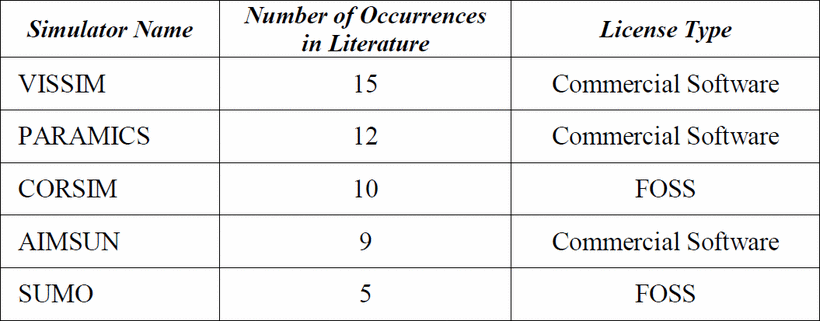
\includegraphics[width=\linewidth]{figuras/popular_trafficsims}
    \begin{tabular}{@{}lcl@{}}
        \textbf{Simulador} & \multicolumn{1}{l}{\textbf{Ocurrencias en Literatura}} & \multicolumn{1}{l}{\textbf{Tipo de Licencia}} \\ \midrule
        VISSIM & 15 & Comercial \\
        PARAMICS & 12 & Comercial \\
        CORSIM & 10 & Libre \\
        AIMSUN & 9 & Comercial \\
        SUMO & 5 & Libre \\ \bottomrule
    \end{tabular}
    \caption[Tabla comparativa simuladores de tráfico.]{Los cinco simuladores más prominentes en la literatura (tabla adaptada de \autocite{traffic_sim_review}).}
    \label{table:prom_trafficsim}
\end{table}

\subsubsection{VISSIM}

VISSIM es un entorno de simulación discreto y microscópico, desarrollado propietariamente por el Grupo PVT en Alemania \autocite{vissim}. Es un simulador generalista, capaz de modelar sistemas de transporte multi-modales, en los que interactúan tanto vehículos ``convencionales'' como bicicletas, tranvías y hasta trenes pesados \autocite{fellendorf2010microscopic}. Modela el movimiento de cada entidad dinámica- y estocásticamente, en instantes discretos de tiempo. 

VISSIM es considerado actualmente el líder en términos de popularidad y número de publicaciones en estudios de sistemas de transporte.

\subsubsection{Aimsun}

Aimsun es un simulador de tráfico con una larga trayectoria, desarrollado por \emph{TSS - Trasport Simulation Systems}, una empresa basada en Barcelona. El desarrollo del simulador comenzó en el año 1989, y actualmente se encuentra en su versión 8.2 \autocite{aimsunweb}.

Aimsun cuenta con la particularidad de ser un entorno integrado micro- y mesoscópico de simulación de tráfico. Esto le da adaptabilidad a los problemas; para redes que requieran detalle del movimiento de sus entidades, se utiliza el modelo macroscópico, mientras que para redes de mayor escala se puede utilizar el modelo mesoscópico.

Este simulador es muy popular en la literatura académica dada su extensibilidad y adaptabilidad a un gran número de escenarios. Sin embargo, existe una crítica común a su complicado nivel de programación de sus redes (se estima un complejidad hasta 8(\textbf{!}) veces mayor que para otros simuladores \autocite{jones2004traffic}), y a su necesidad de meticulosa calibración para obtener resultados realistas \autocite{jones2004traffic,ratrout2009comparative}.

\subsubsection{CORSIM}

TSIS-CORSIM, actualmente en su versión 6.3, es un simulador de tráfico de tipo microscópico desarrollado por el \emph{Centro McTrans} del Instituto de Transportes de la Universidad de Florida \autocite{tsis-corsim}. Al igual que Aimsun, CORSIM es muy popular en la literatura académica, y destaca por ser más apto para el modelamiento de redes de transporte complejas.  

El simulador incluye dos modelos de simulación microscópica distintos - NETSIM para entornos urbanos, y FRESIM para tráfico en carreteras y zonas rurales. Si bien esto significa una mayor especialización y modelos más precisos para cada uno de estos casos, esto viene en desmedro de la posibilidad de simular de manera integrada un entorno que incluya ambas categorías \autocite{jones2004traffic}.

\subsubsection{SUMO}

SUMO, \emph{\textbf{S}imulation of \textbf{U}rban \textbf{MO}bility} \autocite{sumo}, es un simulador de sistemas de transporte desarrollado por el Instituto de Sistemas de Transporte Alemán \autocite{dlr}. 
Es de fuente abierta, y utiliza un modelo microscópico para la simulación de redes de transporte.

Comparado con los simuladores presentados anteriormente, SUMO es relativamente nuevo, y todavía no cuenta con el mismo nivel de soporte y renombre que CORSIM o Aimsun, especialmente en el área de investigación de sistemas de transporte. Sin embargo, su popularidad ha aumentado de manera exponencial los últimos años, y ha ganado relevancia especialmente en estudios de Sistemas Inteligentes de Transporte \autocite{sumo-popularity}, alcanzando el primer lugar en cantidad de publicaciones relacionadas con comunicaciones vehiculares \autocite{sumo-popularity2}. Se especula que esto se debe a su naturaleza abierta, lo cual lo hace más accesible a investigadores, y además significa que es naturalmente extensible y adaptable a nuevos desafíos.

\subsubsection{Paramics}

Paramics, desarrollado por Quadstone Paramics, un subsidiary de Pitney Bowess \autocite{paramics} es un simulador microscópico de redes de transporte. Es capaz de simular el espectro completo de tamaño de redes de transporte - desde intersecciones aisladas a redes de transporte a escala nacional.

El simulador cuenta también con una API de extensión para la implementación de \emph{plugins} enfocados a la integración de aplicaciones de Sistemas Inteligentes de Transporte. Esta API permite interactuar con todos los aspectos de la simulación, desde la simple obtención de datos desde las entidades internas hasta la modificación de los modelos de movilidad internos.

Finalmente, Paramics es además el simulador de preferencia del Área de Transportes del Departamento de Ingeniería Civil de la Universidad de Chile.

\subsection{Simuladores de redes inalámbricas}

Kumar \emph{et al.} realizaron en 2012 un estudio comparativo en el ámbito de Simuladores para Redes Inalámbricas \autocite{networksimcomparativestudy}, trabajo basado parcialmente en el estudio realizado en 2009 por Weingartner, vom Lehn y Wehrle sobre la eficiencia de estos simuladores \autocite{perf_comp_recentnetworksims}. Paralelamente, investigadores de la Universidad de Malasia y la Universidad Carlos III de Madrid, España, publicaron también en 2012 un estudio enfocado específicamente en aquellos entornos de software de fuente abierta para la simulación de redes inalámbricas de sensores \autocite{perf_comp_opensourcenetworksims}.

A continuación se discutirán brevemente las particularidades de los siguientes cuatro entornos de simulación, destacados en los artículos previamente mencionados: GloMoSim/QualNet, OMNeT++, ns-2 y ns-3. Se escogieron específicamente esto simuladores dada su prominencia en dichos estudios y en la literatura académica en general.
 
\subsubsection{GloMoSim}

En primer lugar, GloMoSim es un simulador de fuente abierta desarrollado por investigadores de la Universidad de California, Los Ángeles \autocite{glomosim}. El simulador utiliza las capacidades de simulación de eventos discretos y paralelos otorgadas por el lenguaje de programación Parsec, desarrollado en el Laboratorio de Computación Paralela de la UCLA \autocite{parsec}. QualNet es un derivado comercial de este mismo software, basado en C++ en vez de Parsec. 

Las desventajas de GloMoSim y QualNet son varias. Para nombrar un par, no presentan soporte para un número considerable de implementaciones de TCP, y su interfaz gráfica es deficiente. Finalmente, además GloMoSim ya no se encuentra en desarrollo activo, por lo que es poco probable que esto se solucione en el futuro.

\subsubsection{OMNeT++}

\begin{figure}
    \centering
    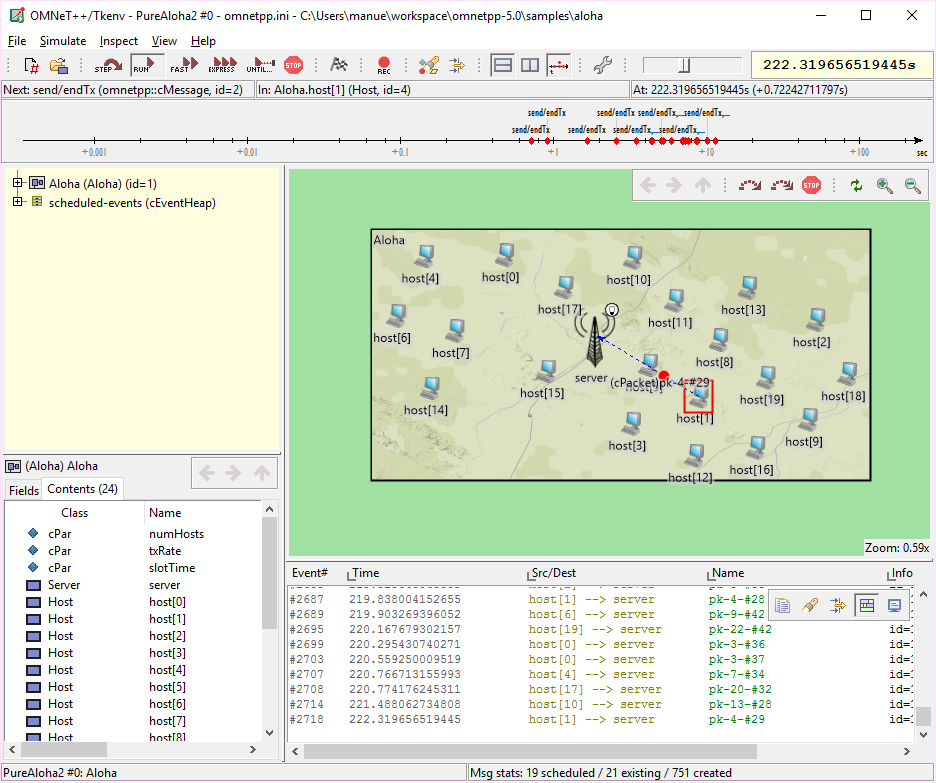
\includegraphics[width=.8\linewidth]{figuras/omnetpp_aloha}
    \caption{Entorno de simulación gráfica de OMNeT++.}
    \label{fig:omnetpp_simgui}
\end{figure}

OMNeT++, \emph{\textbf{O}bjective \textbf{M}odular \textbf{Ne}twork \textbf{T}estbed in C\textbf{++}}, es un entorno modular y basado en componentes para la simulación de sistemas de eventos discretos \cite{omnet2008overview}. Está escrito en C++, y si bien en estricto rigor OMNeT++ en sí sólo conforma el \emph{framework} genérico para la definición de modelos, la distribución incluye además múltiples extensiones para el modelamiento de redes de comunicación -- siendo la principal de éstas INET.

INET incluye modelos para la simulación de múltiples \emph{stacks} de protocolos para la comunicación tanto cableada como inalámbrica, a través de una gran cantidad de protocolos (IPV6, WSN, etc.). Finalmente, INET incluye además modelos de movilidad, para el estudio de redes con nodos en movimiento.

OMNeT++ presenta una gran ventaja en su diseño modular y extensible, y se posiciona como una excelente opción para simulaciones que requieran un alto nivel de flexibilidad.

\subsubsection{ns-2 y ns-3}

ns-2 es un simulador de eventos discretos para la simulación de redes de comunicación, cuyo desarrollo comenzó en 1989 y que a lo largo de los años ha recibido grandes contribuciones tanto de la comunidad científico como de corporaciones como DARPA, Xerox, etc. Gracias a su larga trayectoria y extenso soporte, actualmente cuenta con un gran renombre en academia.

El simulador y sus módulos en sí están escritos en C++, pero se utiliza una extensión del lenguaje Tcl para su configuración y la definición de topologías de red. Esta decisión de diseño fue producto de un deseo de evitar la recompilación del simulador al realizar cambios en algún escenario, lo cual tenía mucho sentido en un tiempo en que la compilación implicaba extensos tiempos de espera. Hoy en día sin embargo, con los avances en potencia computacional, es más una desventaja, perjudicando la escalabilidad del sistema \autocite{perf_comp_recentnetworksims} a cambio de una marginal mejora en tiempos de recompilación. 

ns-3 es considerado el sucesor de ns-2, llevando el exitoso simulador al siglo XXI. A diferencia de su ancestro, ns-3 está escrito completamente en C++, y opcionalmente algunos módulos pueden definirse en Python. Además, ns-3 incluye extensas optimizaciones en términos de escalabilidad y paralelismo, a cambio de una incompatibilidad con antiguos modelos desarrollados para ns-2

\subsection{Entornos de simulación bidireccional}

A continuación se resumirá brevemente el estado del arte en el tema de simulación bidireccional para simulaciones de Sistemas Inteligentes de Transporte. 

\subsubsection{Simulaciones unidireccionales}

De acuerdo a Sommer \emph{et al.} \autocite{sommer2008need}, la mayor parte de las simulaciones de comunicaciones inalámbricas en ITS se hacen a través de la importación de trazas de movimiento reales desde simuladores de transporte, de manera unidireccional. Dichas trazas se pueden generar de dos manera: \textit{offline}, es decir, aisladamente en el simulador de transporte, para luego ser exportadas en un formato que el simulador de red sea capaz de interpretar, y \textit{decoupled online}, de manera que el simulador de transporte genere las trazas en tiempo real y el simulador de red simplemente las ``consume''. Sin embargo, si bien este método permite analizar el efecto del modelo de movimiento de un sistema de transporte en las comunicaciones inalámbricas, es incapaz de reflejar el impacto de la propagación de información del estado del tráfico en el modelo mismo. Es decir, esta metodología no es útil para la simulación de, por ejemplo, sistemas de advertencia de accidentes o de asistencia al conductor, puesto que las trazas de movimiento están predefinidas o se generan sin considerar los resultados de esta comunicación. Este tipo de simulación, si bien es útil para ciertos análisis específicos, no constituye una simulación bidireccional y no abarca la totalidad del problema.

Los trabajos realizados por investigadores de la Universidad Jiao Tong de Shanghai en \autocite{suvnet1,suvnet2} son ejemplos de esta modalidad. Para estas investigaciones, los autores obtuvieron trazas reales de movimiento de SUVnet, una red vehicular compuesta por aproximadamente 4000 taxis en la ciudad de Shanghai. Estas trazas luego fueron simplemente utilizadas en simulaciones de red de comunicaciones para la validación de los modelos desarrollados.

Otro ejemplo de esto es la investigación presentada por Goebel \emph{et al.} en \autocite{omnetv2xtraces}. En este trabajo, los investigadores utilizaron SUMO para la generación de trazas vehiculares realistas, las cuales luego fueron importadas en OMNeT++ para el estudio del impacto de la movilidad vehicular en comunicaciones celulares. 

\subsubsection{Entornos integrados}\label{sec:integrated_sim}

\begin{figure}
    \centering
    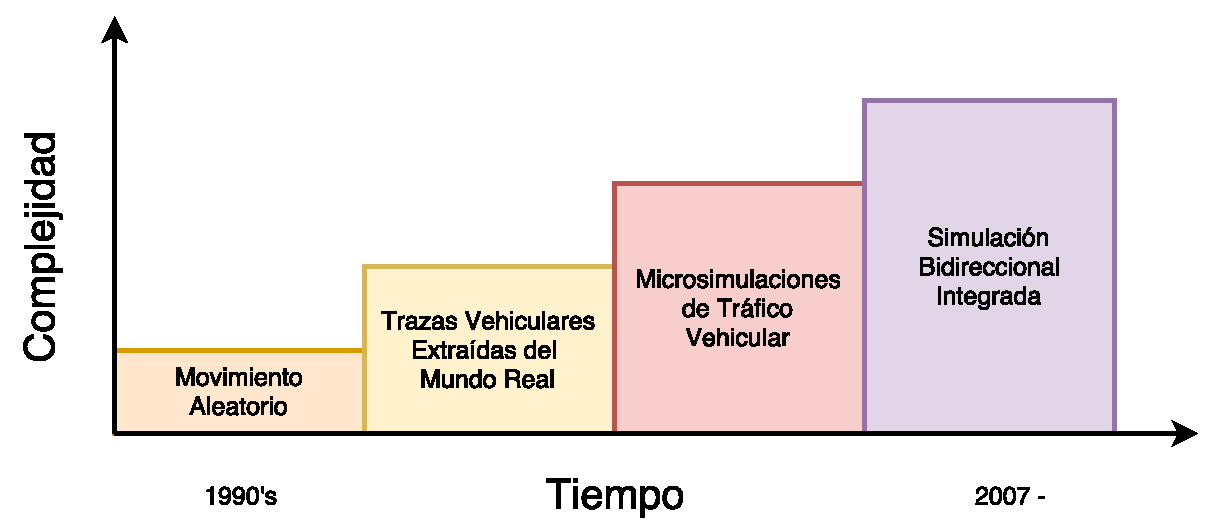
\includegraphics[width=\linewidth]{figuras/sommer_adapted.pdf}
    \caption[Evolución de simulaciones integradas.]{Evolución de simulaciones integradas para ITS (gráfico adaptado de \autocite{sommer_dressler2}).}
    \label{fig:bidir_evol}
\end{figure}

La necesidad de un entorno integrado para la simulación de Sistemas Inteligentes de Transportes es un tema que ha estado presente en la comunidad académica hace casi más de una década ya. En particular, Sommer \emph{et al.} argumentaron fuertemente a favor de la idea en \autocite{sommer2008need} y \autocite{sommer_dressler2}; el siguiente análisis se basa principalmente en ambos documentos, con algunas fuentes adicionales que se mencionarán oportunamente. 

En primer lugar, los autores destacan la existencia de un sistema de simulación bidireccional desarrollado por la Universidad Nacional de Chiao Tung, Taiwan \autocite{nctuns4,nctuns6}, el cual permite la simulación íntegra de un sistema de transportes dotado de capacidades de comunicación inalámbrica. 

NCTUns, actualmente en su versión 6.0 (publicada en junio del 2010 \autocite{nctuns6}), es un simulador para el estudio de Sistemas Inteligentes de Transporte. Su principal particularidad es que presenta un entorno totalmente integrado para la ejecución de dichas simulaciones; es decir, es tanto un simulador de redes de comunicaciones como de tráfico. Incluye capacidades para simular comportamiento tanto autónomo como predefinido (\emph{rutas}) de vehículos, e implementa un \emph{stack} de protocolo completo en cada vehículo.

No obstante, Sommer \emph{et al.} critican la incompatibilidad de dicho sistema (en su versión 4.0) con los modelos de protocolos de comunicación y transporte ya desarrollados para los simuladores más prominentes, limitando su utilidad práctica en la investigación. Además. si bien NCTUns es capaz de simular un número capacidad de capas físicas, todavía se encuentra muy limitado en ese aspecto en comparación con otros simuladores de redes.

Los investigadores mencionan también la existencia de TraNS \autocite{piorkowski2008trans}, un \emph{framework} para la integración de ns-2 con SUMO. Este sistema implementa un \emph{loop} de control y \emph{feedback} activo entre ambos simuladores, estableciendo así una simulación bidireccional que permite la emulación de un ITS.

TraNS integra dos simuladores de renombre en la academia, y ha sido muy bien recibido. Sin embargo, los autores destacan que carece de ciertas funcionalidades -- principalmente, la capacidad de sincronizar y controlar el tiempo de simulación entre ambos simuladores.

Se debe destacar también los trabajos realizados por investigadores en la Universidad Estatal de Nueva York en Buffalo \autocite{zhao2016integrated} y de la Universidad de Düsseldorf \autocite{lochert2005multiple}. Ambos constituyen ejemplos de simulaciones bidireccionales -- no obstante se ven limitados por su especificidad, y dificultad de adaptación a escenarios más diversos. El trabajo de Shalaby en su tesis de magíster \autocite{shalaby} también sufre este mismo problema, además de temas relacionados a la eficiencia del \emph{framework} desarrollado por la autora, principalmente ligados a la elección de mecanismo de comunicación entre los simuladores (archivos en disco).


Finalmente, Sommer, German y Dressler presentan su solución en \autocite{sommer_german_dressler}: VEINS, un \textit{framework} de integración entre OMNeT++ y SUMO. Ambos simuladores se escogieron específicamente por su adopción en el mundo académico, y por sus naturalezas abiertas y fáciles de adaptar y modificar.

A través de VEINS, ambos simuladores se ejecutan en paralelo, comunicándose en tiempo real mediante un \textit{socket} utilizando el protocolo TCP; SUMO proporciona las trazas de movimiento de los elementos en la simulación a la vez que OMNeT++ simula el comportamiento de la red de comunicaciones. Además, mediante este esquema, OMNeT++ también puede modificar directamente el comportamiento del modelo de transporte, por ejemplo alterando la velocidad de un vehículo en respuesta a un mensaje específico obtenido a través de la red de comunicaciones. De esta manera, el \textit{framework} en cuestión permite modelar sistemas complejos y dinámicos, que reflejan de buena manera la realidad.

Sin embargo, VEINS sufre por su elección de simulador de transporte; SUMO todavía se encuentra en una temprana etapa de desarrollo, lo cual implica que frecuentemente sufre de problemas de estabilidad y de falta de características y documentación. Por ejemplo, hasta diciembre del 2015 (versión 0.25.0), SUMO no contaba con un editor gráfico de redes de transporte\footnote{\url{http://sumo.dlr.de/wiki/FAQ}}, lo cual dificultaba mucho el diseño de redes originales. Además, la curva de aprendizaje de SUMO es bastante pronunciada, y todas sus configuraciones son a través de archivos; es por esto que en muchos departamentos de ingeniería de transporte se opta por otros simuladores más avanzados y estables.



\chapter{Diseño, Metodología y Funcionalidad Implementada}
\section{Diseño Arquitectural}\label{sec:architecture}

El software desarrollado consiste en un \emph{plugin} que extiende la funcionalidad de Paramics, agregándole la capacidad de comportarse como un servidor TraCI. Específicamente, el \emph{plugin} consiste en una implementación parcial de un servidor TraCI, el cual interpreta mensajes entrantes a través de un \emph{socket} TCP, ejecuta las acciones solicitadas, y responde a través del mismo medio (figura \ref{fig:pveins_genarch}).

\begin{figure}[h]
    \centering
    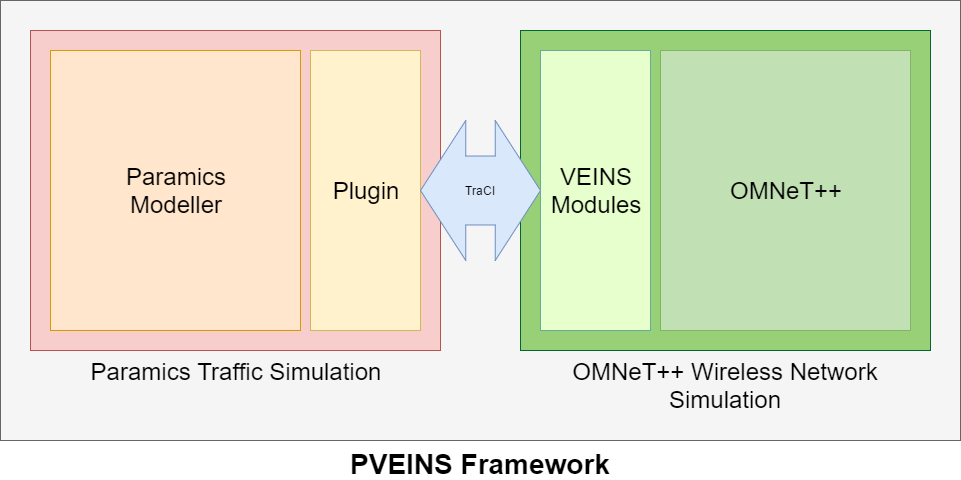
\includegraphics[width=\linewidth]{figuras/PVEINSArch.png}
    \caption{Visión macroscópica del framework; el plugin desarrollado actúa como una interfaz entre TraCI y Paramics.}
    \label{fig:pveins_genarch}
\end{figure}

A nivel más microscópico, la arquitectura del \emph{framework} se desarrolló en dos versiones distintas, la primera de éstas siendo descartada al realizar las pruebas de validación del proyecto. A continuación, se describirán brevemente estas dos iteraciones del diseño del software, destacando principalmente las razones del descarte de la versión preliminar.

\subsubsection{Arquitectura preliminar}

Originalmente, el \emph{framework} se implementó como un hilo de ejecución (un \emph{thread}) paralelo a Paramics. La principal ventaja de este diseño era evitar el bloqueo de la interfaz del simulador al encontrarse el servidor TraCI bloqueado esperando mensajes entrantes en el \emph{socket}. 

Un diagrama de la arquitectura general de esta implementación puede observarse en la figura \ref{fig:ptraci_arch}. Al iniciarse Paramics, el \emph{plugin} inicializaba el servidor en un \emph{thread} paralelo; el servidor luego se enlazaba a un \emph{socket} TCP y se bloqueaba en espera de mensajes entrantes desde un cliente TraCI (en nuestro caso, VEINS). Al recibir una serie de comandos TraCI, el servidor los interpretaba, comunicándose con Paramics a través de su API, obteniendo datos y modificando el estado de la simulación. El servidor interpretaba todos los comandos en un mensaje TraCI antes de enviar todos los mensajes de respuesta correspondientes en un único mensaje TraCI.

Esta arquitectura funcionaba de manera eficiente y permitía la ejecución de la simulación de Paramics completamente sin la intervención del usuario (ya que el \emph{thread} mismo del \emph{plugin} era capaz de llamar el método de inicio de simulación). 

Sin embargo, al comenzar a realizar pruebas con redes de tamaño más extenso se presentó un problema imprevisto, y -- a la larga -- irreparable sin acceso al código fuente de Paramics. El problema radicaba en la función de avance de simulación definido en la API de Paramics, \texttt{qps\_GUI\_runSimulation()}, la cual, como se descubrió más tarde, también actualiza la interfaz gráfica de el modelador de Paramics a través de llamados a la librería Qt4 \cite{qt}. Estos llamados no son \emph{thread-safe}\footnote{Es decir, no incluyen medidas para asegurar el acceso exclusivo de recursos a un sólo \emph{thread}.}, y en redes grandes de Paramics generan \emph{data races} al ser invocados desde un \emph{thread} paralelo al principal del simulador. Esto finalmente generaba corrupción de memoria en el motor gráfico (principalmente, lecturas de direcciones inválidas de memoria), lo cual causaba un error fatal en la simulación.

Se estudiaron múltiples maneras de resolver este problema manteniendo la estructura paralela del \emph{plugin} sin éxito, ya que la única manera confiable de forzar un avance de la simulación desde el \emph{plugin} es a través de la función anteriormente mencionada. Se decidió entonces abordar el problema desde un ángulo distinto, enfoque que se discutirá en la siguiente sección.

\begin{figure}[]
    \centering
    \begin{sequencediagram}
    \newthread{D}{OMNeT++}{}
    \newinst[1]{A}{VEINS}{}
    \newinst[3]{B}{Plugin (TraCIServer)}{}
    \newthread[2]{C}{Paramics}{}
    
    \begin{messcall}{C}{run()}{B}
        \postlevel
        \begin{call}{B}{waitForCommands()}{B}{}
        \end{call}
    \end{messcall}
    
    \begin{call}{D}{Solicitud}{A}{Resultado}
    
        \begin{call}{A}{Comando TraCI}{B}{Respuesta TraCI}
            \begin{call}{B}{parseCommand()}{B}{sendResponse()}
                \postlevel
                \begin{call}{B}{API Paramics}{C}{Datos}
                \end{call}
                \postlevel
            \end{call}
        \end{call}
    \end{call}
\end{sequencediagram}
    \caption{Arquitectura preliminar}
    \label{fig:ptraci_arch}
\end{figure}

\subsubsection{Arquitectura final} \label{sec:architecture:final}

El problema presentado por la incompatibilidad de \texttt{qps\_GUI\_runSimulation()}, función de avance de simulación de la API de Paramics, con múltiples \emph{threads} implicó la necesidad de reevaluar la arquitectura general del \emph{framework} en su totalidad. Se decidió descartar la idea de un \emph{thread} paralelo para el servidor, y se implementó un esquema secuencial de interpretación de mensajes TraCI, utilizando \emph{loops} bloqueantes para controlar la ejecución de pasos de simulación.

Esta arquitectura puede visualizarse en la figura \ref{fig:ptraci_arch2}. Al principio de cada paso de simulación, el simulador invoca la función \texttt{qpx\_CLK\_startOfSimLoop()}, definida en el \emph{plugin}, antes de realizar cualquier otra acción. Esta función a su vez invoca el método \texttt{preStep()} del servidor, dentro del cual se ejecuta un \emph{loop} de interpretación de comandos TraCI (y de envío de respuestas a éstos). Este \emph{loop} se interrumpe al recibir un mensaje de paso de simulación, retornando así de \texttt{preStep()} y \texttt{qpx\_CLK\_startOfSimLoop()}, y liberando al simulador para que realice su procedimiento interno de avance de simulación. 

Luego de realizar el avance de simulación, Paramics invoca la función \texttt{qpx\_CLK\_endOfSimLoop()}, también definida en el \emph{plugin}. Esta invoca a su vez el método \texttt{postStep()} del servidor, el cual se encarga de realizar la recolección de datos post-paso de simulación, de terminar de interpretar eventuales comandos recibidos previo al paso de simulación y de enviar respuestas pendientes al cliente. Finalmente, esta función retorna el control de la ejecución a Paramics, y el ciclo comienza nuevamente.

Mediante esta arquitectura se logró eliminar por completo el problema presentado por \texttt{qps\_GUI\_runSimulation()}, obteniendo incluso una leve mejora en rendimiento respecto al diseño antiguo, dado que, ya que todo corre en un sólo \emph{thread}, se evita el uso de elementos de sincronización, los cuales pueden agregar \emph{overhead} al procedimiento.

Este nuevo diseño presenta una única desventaja: es necesario el inicio de la simulación de manera manual por parte del usuario, luego de lo cual funciona de manera autónoma. Esto ya que no existe manera de iniciar el \emph{loop} de simulación de Paramics a través de la API sin recurrir a \emph{threads}.

Finalmente, se debe notar que dada la representación en tiempo discreto de los pasos de simulación, el avance de esta en muchos casos no alcanza exactamente el tiempo deseado. Si definimos el paso de simulación como $\triangle T$, el instante de tiempo en que se recibe el comando de avance como $T_{i}$ y el instante de tiempo objetivo $T_{o}$, la simulación se avanzará un número $n \in \mathbb{N}$ de pasos, tal que

\[ T_{i} + (n \times \triangle T) = T_{f} \]
\[ T_{i} + ((n - 1) \times \triangle T) = T_{f}' \]
\[ T_{f} \geq T_{o} \]
\[ T_{f}' < T_{o} \]

En otras palabras, la simulación se avanzará el mínimo número de pasos tal que el tiempo final es \emph{igual o mayor} al instante de tiempo objetivo. Esto es para asegurar que se ejecuten todas las acciones que dependan del tiempo de simulación por lo menos hasta dicho instante.

\begin{figure}[]
    \centering
    \begin{sequencediagram}
    \newthread{B}{Paramics + Plugin}{}
    \newthread[7]{A}{OMNeT++/VEINS}{}

    \begin{sdblock}{Loop de simulación}{}
        \postlevel
        \begin{call}{B}{\texttt{qpx\_CLK\_startOfSimLoop()}}{B}{}
            \begin{sdblock}{Loop pre-simulación}{}
                \begin{call}{B}{\texttt{server->preStep()}}{B}{Comando: Paso de Simulación}
                    \begin{call}{A}{Mensajes TraCI}{B}{Respuestas TraCI}
                        \postlevel
                    \end{call}
                \end{call}
            \end{sdblock}
        \end{call}
        \begin{sdblock}{Paso de simulación}{}
            \postlevel
            \postlevel
            \begin{call}{B}{\begin{minipage}{8cm}
                        Actualización de estado:
                        \begin{itemize}
                            \item Salida y llegada de vehículos
                            \item Modificación de velocidades y rutas
                        \end{itemize}
                \end{minipage}}{B}{}
            \end{call}
        \end{sdblock}
        \postlevel
        \begin{call}{B}{\texttt{qpx\_CLK\_endOfSimLoop()}}{B}{}
            \begin{sdblock}{Loop post-simulación}{}
                \begin{call}{B}{\texttt{server->postStep()}}{B}{Fin de Comandos}
                    \begin{call}{A}{Mensajes TraCI}{B}{Respuestas TraCI}
                        \postlevel
                    \end{call}
                \end{call}
            \end{sdblock}
        \end{call}
    \end{sdblock}
\end{sequencediagram}
    \caption{Arquitectura final del \emph{framework}}
    \label{fig:ptraci_arch2}
\end{figure}
\newpage
\section{Metodología de desarrollo} \label{sec:metodologia}

El desarrollo del \emph{plugin} se llevó a cabo de manera iterativa, implementando funcionalidades esenciales en primera instancia, y luego construyendo sobre esta base, cuidando en cada paso de no pasar a llevar las funcionalidades previamente implementadas y perfeccionando implementaciones anteriores. El orden de desarrollo de las funcionalidades fue cuidadosamente planeado, tomando en cuenta que en muchos casos se requería un orden específico de implementación de funcionalidades; \emph{e.g.} era imperativo el desarrollo de la funcionalidad de obtención de variables de vehículos antes de poder implementar suscripciones, ya estas últimas dependen de la funcionalidad de la primera. Las etapas generales de desarrollo que se siguieron fueron:

\begin{enumerate}
    \item En primer lugar, se desarrolló la base de comunicaciones del \emph{framework}, es decir, comunicación con el \emph{socket}, recepción e interpretación de mensajes. 
    
    \item A continuación, se implementó la funcionalidad esencial de control de simulación (los comandos presentados en la sección \ref{sec:comandos:controlsim}), con el fin de poder establecer una primera conexión con un cliente TraCI y simplemente ejecutar una simulación sin otros comandos. 
    El protocolo define un ``\emph{handshake}'' consistente en la verificación de versiones de TraCI compatibles entre cliente y servidor, por lo que el correcto funcionamiento del comando de obtención de versión fue prioridad en esta etapa.
    
    \item En tercer lugar se implementaron los comandos de obtención de variables de la simulación. Teniendo ya la base de comunicaciones funcionando, la implementación de éstos fue mucho más directa.
    
    \item Cuarto, sobre la implementación de los comandos de obtención de variables, se desarrollaron los distintos tipos de suscripciones disponibles.
    
    \item Finalmente, en última instancia, se desarrollaron los comandos de modificación de estados, ya que éstos necesariamente requerían una fundación sólida dada su relativa complejidad.
\end{enumerate}

Cabe destacar que, pese a la cuidadosa planificación realizada previa al desarrollo del \emph{framework} (y como siempre sucede en el desarrollo de \emph{software}), en muchas oportunidades fue necesario volver a un paso anterior para rediseñar o mejorar una implementación. El principal ejemplo de ésto es el rediseño de la arquitectura general del \emph{plugin}, detallado en la sección \ref{sec:architecture}, el cual implicó el rediseño y posterior reimplementación de gran parte de las etapas 1 (base de comunicaciones) y 2 (funcionalidad de control de simulación) del \emph{plugin}.

En términos de control de versiones y manejo del historial del desarrollo se escogió utilizar el sistema \emph{git} \autocite{git}, dada su popularidad, extenso soporte y documentación y la familiaridad del memorista con este sistema. El servicio de \emph{hosting} específico escogido para sistema fue \emph{GitHub} \autocite{github}; el código fuente del proyecto puede encontrarse en el perfil personal del autor \autocite{molguin_github}, en el repositorio \autocite{pveins_github}.
\newpage
\section{Funcionalidad Implementada}

El protocolo TraCI define más de 30 comandos distintos, cada uno con una gran cantidad de variables y parámetros asociados (ver apéndice \ref{anex:traci} para una descripción más detallada del funcionamiento de este protocolo). Implementar esta gran cantidad de funcionalidades no hubiese sido factible, por lo que se escogió un subconjunto acotado de éstas a implementar, considerando en específico aquellos comandos esenciales para simulaciones de ITS.

\subsection{Comandos Implementados} \label{sec:comandos}

\subsubsection{Comandos de Control de Simulación}

\begin{itemize}
    \begin{multicols}{2}
        \mcitem{\texttt{0x00} Obtención de Versión}
        \mcitem{\texttt{0x02} Avance de Simulación}
        \mcitem{\texttt{0xff} Cierre de Conexión}
    \end{multicols}
\end{itemize}

\subsubsection{Comandos de Obtención de Variables}

\begin{description}[style=multiline]
    
    \item[\texttt{0xa4}] Variables de vehículos
    \begin{multicols}{2}
        \begin{itemize}
            \mcitem{\texttt{0x00} Lista de vehículos activos en la red}
            \mcitem{\texttt{0x01} Número de vehículos activos en la red}
            \mcitem{\texttt{0x36} Inclinación actual}
            \mcitem{\texttt{0x39} Posición actual (3D)}
            \mcitem{\texttt{0x40} Velocidad actual}
            \mcitem{\texttt{0x42} Posición actual (2D)}
            \mcitem{\texttt{0x43} Ángulo actual}
            \mcitem{\texttt{0x44} Largo}
            \mcitem{\texttt{0x4d} Ancho}
            \mcitem{\texttt{0x4f} Tipo de vehículo}
            \mcitem{\texttt{0x50} Calle actual}
            \mcitem{\texttt{0x51} Identificador de pista actual}
            \mcitem{\texttt{0x52} Índice de pista actual}
            \mcitem{\texttt{0xbc} Altura}
        \end{itemize}
    \end{multicols}
    
    \item[\texttt{0xa5}] Variables de tipos de vehículos
    \begin{multicols}{2}
        \begin{itemize}
            \mcitem{\texttt{0x00} Lista de tipos definidos}
            \mcitem{\texttt{0x01} Número de tipos definidos}
            \mcitem{\texttt{0x41} Velocidad máxima}
            \mcitem{\texttt{0x44} Largo}
            \mcitem{\texttt{0x46} Aceleración máxima}
            \mcitem{\texttt{0x47} Deceleración máxima}
            \mcitem{\texttt{0x4d} Ancho}
            \mcitem{\texttt{0xbc} Altura}
        \end{itemize}
    \end{multicols}
    
    \item[\texttt{0xa6}] Variables de rutas
    \begin{multicols}{2}
        \begin{itemize}
            \mcitem{\texttt{0x00} Lista de rutas definidas}
            \mcitem{\texttt{0x01} Número de rutas definidas}
            \mcitem{\texttt{0x54} Arcos (calles) componentes de la ruta}
        \end{itemize}
    \end{multicols}
    
    \item[\texttt{0xa8}] Variables de polígonos (edificios y estructuras)
    \begin{multicols}{2}
        \begin{itemize}
            \mcitem{\texttt{0x00} Lista de polígonos}
            \mcitem{\texttt{0x01} Número de polígonos}
        \end{itemize}
    \end{multicols}
    
    Cabe notar que Paramics no maneja edificios en sus simulaciones, al menos no edificios accesibles a través de la API de programación, por lo que estos métodos se implementaron de manera que reportan siempre 0 polígonos en la simulación.
    
    \item[\texttt{0xa9}] Variables de nodos (intersecciones) de la red
    \begin{multicols}{2}
        \begin{itemize}
            \mcitem{\texttt{0x00} Lista de intersecciones}
            \mcitem{\texttt{0x01} Número de intersecciones}
            \mcitem{\texttt{0x42} Posición de la intersección}
        \end{itemize}
    \end{multicols}
    
    \item[\texttt{0xaa}] Variables de arcos (calles) de la red
    \begin{multicols}{2}
        \begin{itemize}
            \mcitem{\texttt{0x00} Lista de calles}
            \mcitem{\texttt{0x01} Número de calles}
        \end{itemize}
    \end{multicols}
    
    \item[\namedlabel{item:simvars}{\texttt{0xab}}] Variables de Simulación
    \begin{multicols}{2}
        \begin{itemize}
            \mcitem{\texttt{0x70} Tiempo de simulación}
            \mcitem{\texttt{0x73} Número de vehículos liberados a la red en el último paso de simulación}
            \mcitem{\texttt{0x74} Lista de vehículos liberados a la red en el último paso de simulación}
            \mcitem{\texttt{0x79} Número de vehículos que han llegado a su destino en el último paso de simulación}
            \mcitem{\texttt{0x7a} Lista de vehículos que han llegado a su destino en el último paso de simulación}
            \mcitem{\texttt{0x7b} Tamaño del paso de simulación}
            \mcitem{\texttt{0x7c} Coordenadas de los límites de la red vehicular}
        \end{itemize}
    \end{multicols}
    
    Las variables \texttt{0x75}, \texttt{0x76}, \texttt{0x77} y \texttt{0x78}, correspondientes a los números y listas de vehículos que comienzaron y terminaron de teletransportarse en el último paso de simulación, así como las variables \texttt{0x6c}, \texttt{0x6d}, \texttt{0x6e} y \texttt{0x6f}, las cuales corresponden a números y listas de vehículos que comenzaron y terminaron de estar estacionados, fueron implementadas ``parcialmente''. En estricto rigor, los mecanismos subyacentes no se implementaron porque no se consideraron críticos, pero se implementó una respuesta \emph{dummy} de 0 vehículos para asegurar su funcionamiento con VEINS.
    
\end{description}

\subsubsection{Comandos de modificación de estado}\label{sec:mod_state}

\begin{description}[style=multiline]
    \item [\texttt{0xc4}] Variables de vehículo
    \begin{multicols}{2}
        \begin{itemize}
            \mcitem{\texttt{0x13} Cambio de pista}
            \mcitem{\texttt{0x14} Cambio de velocidad (lineal)}
            \mcitem{\texttt{0x40} Cambio de velocidad (instantáneo)}
            \mcitem{\texttt{0x41} Cambio de velocidad máxima}
            \mcitem{\texttt{0x45} Coloreado}
            \mcitem{\texttt{0x57} Cambio de ruta (a una lista de arcos otorgada por el cliente)}
            
        \end{itemize}
    \end{multicols}
\end{description}
\chapter{Implementación}
%\section{Organización Lógica del Código}

El código del \emph{plugin} se separó en una serie de módulos lógicos que encapsulan y abstraen cada uno una categoría de funcionalidades de la interfaz con TraCI. De esta manera, se logró una separación lógica de las funcionalidades implementadas, y se simplifican futuras extensiones al código. La organización en archivos de éstos módulos puede observarse en la figura \ref{fig:dirtree}.

Cabe notar también que se utilizó el \emph{namespace} \texttt{traci\_api} para agrupar los elementos propios del framework. 

\begin{figure}[h]
    \dirtree{%
        .1 src/.
        .2 plugin.c\DTcomment{Archivo de inicio del \emph{plugin}}.
        .2 TraCIAPI/\DTcomment{Implementación de la API}.
        .3 Constants.h\DTcomment{Constantes utilizadas en el sistema}.
        .3 Exceptions.h\DTcomment{Excepciones propias del framework}.
        .3 Network.\{cpp/h\}\DTcomment{Métodos de interacción con la red vehicular}.
        .3 Simulation.\{cpp/h\}\DTcomment{Métodos de interacción con la simulación vehicular}.
        .3 Subscriptions.\{cpp/h\}\DTcomment{Suscripciones TraCI}.
        .3 TraCIServer.\{cpp/h\}\DTcomment{Módulo principal, manejo de conexiones TraCI}.
        .3 Triggers.\{cpp/h\}\DTcomment{Operaciones disparadas (temporales o situacionales)}.
        .3 Utils.\{cpp/h\}\DTcomment{Funciones auxiliares y de conveniencia}.
        .3 VehicleManager.\{cpp/h\}\DTcomment{Métodos de interacción con vehículos}.
        .2 shawn/\DTcomment{Archivos externos}.
        .3 socket.\{cpp/h\}\DTcomment{Manejo simplificado de \emph{sockets} TCP}.
        .3 storage.\{cpp/h\}\DTcomment{Manejo simplificado de paquetes de datos}.
    }
    \caption{Estructura de archivos del código fuente del framework.}
    \label{fig:dirtree}
\end{figure}
\newpage
\subsection{plugin.c}\label{sec:plugin.c}

Si bien en estricto rigor no es un módulo del \emph{framework}, merece ser mencionado al ser el archivo principal del \emph{plugin} desarrollado. En este archivo se definen las funciones de extensión y \emph{override} (prefijos \texttt{QPX} y \texttt{QPO}, ver apéndice \ref{anex:paramics_api} para un detalle sobre la API de Paramics) a ser invocadas por Paramics. A continuación se describirán brevemente las más importantes de estas funciones, mientras que el archivo \texttt{plugin.c} puede estudiarse en su totalidad en el código \ref{code:pluginc} en los anexos.

\subsubsection{\texttt{void qpx\_NET\_postOpen()}}\label{sec:qpx_postopen}

Invocada inmediatamente luego de que Paramics carga la red y el \emph{plugin}, esta función inicializa el servidor TraCI. Para esto, crea un \emph{thread} donde corre una función auxiliar \texttt{runner\_fn()}, la cual se encarga de:

\begin{enumerate}
    \item Obtener el puerto en el cual esperar conexiones entrantes desde los parámetros de ejecución de Paramics. De no haberse especificado puerto, utiliza uno por defecto.
    \item Inicializar un objeto \texttt{TraCIServer} (ver sección \ref{sec:traciserver}) encargado de las conexiones entrantes en el puerto anteriormente definido.
\end{enumerate}

\subsubsection{\texttt{void qpx\_CLK\_startOfSimLoop()} y \texttt{void qpx\_CLK\_endOfSimLoop()}}

Estas funciones se ejecutan antes y después de cada paso de simulación respectivamente, y llaman a los procedimientos correspondientes en el servidor, los método \texttt{preStep()} y \texttt{postStep()}. Ver sección \ref{sec:traciserver} para más detalle sobre estos métodos y el avance de simulación en general.

\subsubsection{\texttt{void qpx\_VHC\_release(\dots)} y \texttt{void qpx\_VHC\_arrive(\dots)}}

\texttt{qpx\_VHC\_release(VEHICLE* vehicle)} es invocada por Paramics cada vez que un vehículo es liberado a la red de transporte. Simplemente se encarga de notificar al \texttt{VehicleManager} (ver sección \ref{sec:vehiclemanager}) para su inclusión en el modelo interno del \emph{plugin}.

Por otro lado, \texttt{qpx\_VHC\_arrive(VEHICLE* vehicle, LINK* link, ZONE* zone)} es invocada cuando un vehículo alcanza su destino final, y notifica al \texttt{VehicleManager} para eliminar el vehículo en cuestión de la representación interna.

\subsubsection{\texttt{int qpo\_RTM\_decision(\dots)}}\label{sec:plugin.c:decision}

Esta función de \emph{override} es llamada por el núcleo de simulación de Paramics cada vez que un vehículo necesita evaluar su elección de ruta, y debe retornar el índice de la siguiente salida que el vehículo debe tomar (o 0 si se desea mantener la ruta por defecto). En el \emph{plugin} se utiliza para aplicar rutas personalizadas otorgadas por el cliente TraCI.

\subsubsection{\texttt{void qpx\_VHC\_transfer(\dots)}}

Este método es ejecutado por Paramics cada vez que un vehículo pasa de una calle a otra, y se utiliza para determinar si es necesario recalcular la ruta del vehículo en cuestión.

\subsubsection{\texttt{float qpo\_CFM\_leadSpeed(\dots)} y \texttt{float qpo\_CFM\_followSpeed(\dots)}}\label{sec:plugin.c:speed}

Estas funciones se invocan en cada paso de simulación para cada vehículo en la simulación de tráfico de Paramics -- \texttt{leadSpeed()} se invoca para aquellos vehículos que no tienen otro vehículo delante, mientras \texttt{followSpeed()} es invocada los vehículos que se encuentran detrás de otro.

Estas funciones deben retornar la rapidez que se le deberá aplicar al vehículo en cuestión en el siguiente paso de simulación. En el \emph{framework}, se utilizan para aplicar cambios de velocidad dictados por comandos TraCI.
\newpage
\subsection{TraCIServer}\label{sec:traciserver}

Implementa el funcionamiento base del servidor TraCI. Es el primer módulo como tal en inicializarse, y tiene como funciones:

\begin{enumerate}
    \item Asociarse a un \emph{socket} TCP, y esperar una conexión de un cliente TraCI.
    \item Mientras exista una conexión abierta, recibir e interpretar comandos TraCI entrantes.
    \item Enviar mensajes de estado y respuesta a comandos TraCI.
    \item Al recibir un comando de cierre, finalizar la simulación y cerrar el \emph{socket}.
\end{enumerate}

El módulo en cuestión se implementó como una clase de C++ en los archivos \href{https://github.com/molguin92/paramics_traci/blob/master/src/TraCIAPI/TraCIServer.h}{/src/TraCIAPI/TraCIServer.h} y \href{https://github.com/molguin92/paramics_traci/blob/master/src/TraCIAPI/TraCIServer.cpp}{/src/TraCIAPI/TraCIServer.cpp}, y se crea una instancia en el archivo \href{https://github.com/molguin92/paramics_traci/blob/master/src/plugin.c}{plugin.c}.

Cabe destacar que para facilitar el uso de \emph{sockets} y la obtención y envío de datos a través de éstos, se utilizaron las clases \texttt{tcpip::Socket} y \texttt{tcpip::Storage}, definidas en los archivos \href{https://github.com/molguin92/paramics_traci/blob/master/src/shawn/socket.h}{src/shawn/socket.\{cpp/h\}} y \href{https://github.com/molguin92/paramics_traci/blob/master/src/shawn/storage.h}{src/shawn/storage.\{cpp/h\}}. \texttt{tcpip::Socket} abstrae el funcionamiento de un \textit{socket} TCP, y provee métodos de conveniencia que permiten leer y escribir mensajes TraCI completos como objetos \texttt{tcpip::Storage}. Estos a su vez proveen métodos para escribir y leer todo tipo de variables en dichos mensajes, sin la necesidad de hacer la conversión manual a bytes.

Estos archivos no fueron desarrollados por el memorista, sino que fueron obtenidos desde el código fuente de SUMO \footnote{Fuente SUMO: \url{https://github.com/planetsumo/sumo/tree/master/sumo/src/foreign/tcpip}. Debe notarse que, a su vez, los creadores de SUMO originalmente obtuvieron dichos archivos del código fuente del simulador de eventos discretos para redes de sensores \emph{SHAWN} \cite{kroller2005shawn}. Su fuente original se encuentra en \url{https://github.com/itm/shawn/tree/master/src/apps/tcpip}}, distribuidos bajo una licencia BSD\footnote{Licencia clases \texttt{tcpip::Socket} y \texttt{tcpip::Storage}: \url{http://sumo.dlr.de/wiki/Libraries_Licenses\#tcpip_-_TCP.2FIP_Socket_Class_to_communicate_with_other_programs}}.

A continuación se detalla la implementación de las funcionalidades anteriormente mencionadas.

\subsubsection{Inicio de conexión TraCI}

Como se mencionó en la sección \ref{sec:qpx_postopen}, al iniciarse el \emph{plugin} se crea un nuevo \emph{thread}, en el cual se crea una instancia de un objeto de la clase \texttt{TraCIServer}, al cual se le invoca su método \texttt{waitForConnection()} (código \ref{cod:traciserver_waitforconnection}).

\lstinputlisting[float=t, style=CPP, label={cod:traciserver_waitforconnection}, caption={Rutina de inicio de conexión.}]{codigo/traciserver_waitforconnection.cpp}
%\minipagelisting{codigo/traciserver_run.cpp}{Rutina de inicio de conexión.}{cod:traciserver_run}

Este método es simple: imprime información pertinente sobre el \emph{plugin} en la ventana de información de Paramics, y luego espera a recibir una conexión entrante. Es además el único del \emph{framework} que corre en un \emph{thread} paralelo a Paramics en la arquitectura final. Se decidió implementarlo de esta manera para que el inicio de Paramics fuera más fluido y no se bloqueara la interfaz mientras el servidor espera una conexión desde un cliente TraCI.

\subsubsection{Recepción e interpretación de comandos entrantes}

Como se explicó en la sección \ref{sec:architecture:final}, la interpretación de comandos entrantes y el avance del \emph{loop} de simulación se realizan en dos etapas; una previa al paso de simulación y una posterior a éste. Los métodos encargados de esto son \texttt{preStep()} y \texttt{postStep()}, los cuales se detallarán a continuación.

\subsubsection{\texttt{preStep()}}

El método \texttt{preStep()} es invocado por Paramics al principio de cada iteración del \emph{loop} de simulación, antes de ejecutar cualquier otra función. Este método se encarga de recibir mensajes nuevos entrantes a través del \emph{socket} desde el cliente TraCI, e interpreta los comandos dentro de un \emph{loop}. La implementación de éste método puede observarse en los apéndices, código \ref{cod:traciserver_prestep}.

Nótese que \texttt{preStep()} continuamente interpreta, ejecuta y responde a comandos, y sólo retorna al recibir un comando de avance de simulación. De esta manera, retorna el control de la ejecución a Paramics, y el simulador mismo se encarga de realizar el paso de simulación.

En términos de la interpretación de los mensajes, al recibir datos entrantes, el \emph{socket} retorna un objeto \texttt{tcpip::Storage} con el mensaje completo. Luego, en un \emph{loop} adicional, este mensaje se separa en sus comandos TraCI constituyentes, copiando la información perteneciente a cada comando en otro objeto \texttt{tcpip::Storage} temporal. Este objeto se entrega como parámetro al método \texttt{parseCommand()} para la interpretación del comando, luego de lo cual se limpia y se vuelve a utilizar para el siguiente comando.

Finalmente, interpretados todos los comandos, se envía la respuesta al cliente a través del mismo \emph{socket} y se limpian los objetos \texttt{tcpip::Storage} para su reutilización en una nueva iteración del \emph{loop} interno.

\subsubsection{postStep()} \label{sec:poststep}

Al recibir un comando de avance de simulación, \texttt{preStep()} inmediatamente retorna el control del flujo del programa a Paramics. El simulador entonces avanza la simulación, y luego ejecuta el método \texttt{postStep()} del servidor. Al igual que para \texttt{preStep()}, el código de éste método se puede encontrar en los anexos, código \ref{cod:traciserver_poststep}.

Este método tiene como fin la recopilación de las eventuales suscripciones existentes (ver sección \ref{sec:subs}), la interpretación de los comandos restantes en el último mensaje recibido antes del comando de avance de simulación y el envío de eventuales respuestas al cliente. Finalmente, este método retorna, y Paramics vuelve a iniciar una nueva iteración del \emph{loop} de simulación y a ejecutar \texttt{preStep()}.

Cabe notar que \texttt{postStep()} sólo se ejecuta inmediatamente después de la ejecución de un paso de simulación por parte de Paramics, y por ende no se ejecuta si nunca se recibe un comando de avance de simulación.

\subsubsection{Interpretación de comandos TraCI}

Como se mencionó anteriormente, la interpretación de los comandos se lleva a cabo en el método \texttt{parseCommand()}, el cual recibe un único comando encapsulado en un objeto \texttt{tcpip::Storage}. Este método tiene una única misión: interpretar el identificador del comando recibido y delegar su ejecución al método correspondiente de la clase \texttt{TraCIServer}. Su implementación es simple, y su esqueleto puede observarse en el código \ref{cod:traciserver_parsecommand}. En específico, el código del método se puede dividir en dos ramas de ejecución; en caso de comando de suscripción (cuyos identificadores se encuentran todos en el rango $[\texttt{0xd0}, \texttt{0xdb}]$) se extraen los parámetros de la suscripción y se invoca el método \texttt{addSubscription()} para la subsecuente validación y activación de ésta. Por el contrario, en caso de recibir un comando con identificador fuera de dicho rango, se procede a verificar su tipo mediante un \emph{switch}. Cada caso se relaciona con un comando y método específico a invocar, y en caso de no encontrarse el identificador en cuestión se notifica al cliente que el comando deseado no está implementado.

\begin{figure}[htpb]
    \lstinputlisting[style=CPP, label={cod:traciserver_parsecommand}, caption={Esqueleto de \texttt{parseCommand()}}]{codigo/traciserver_parsecommand.cpp}
\end{figure}

Se definieron una serie de métodos en \texttt{TraCIServer} encargados de obtener variables de la simulación o modificar el estado de ésta. El funcionamiento de los métodos es idéntico en todos los casos (a excepción de \texttt{cmdGetPolygonVar()}), y se limita al siguiente procedimiento (ver ejemplo en el código \ref{cod:traciserver_cmdgetvhcvar}):

\begin{enumerate}
    \item Obtener el valor desde el módulo apropiado (por ejemplo, \texttt{VehicleManager} para variables de vehículos, \texttt{Simulation} para variables de la simulación, etc.).
    \item En caso de error en la obtención de los datos (variable no implementada, objeto no existente, etc.), atrapar el error y determinar el curso de acción apropiado (por ejemplo, notificar al cliente).
    \item Finalmente, enviar un mensaje de estado de la solicitud y, en caso de éxito, el valor de la variable, al cliente.
\end{enumerate}

\begin{figure}[htpb]
    \lstinputlisting[style=CPP, label={cod:traciserver_cmdgetvhcvar}, caption={Ejemplo de método de obtención y empaquetado de variables en \texttt{TraCIServer}}]{codigo/cmdGetVhcVar.cpp}
\end{figure}

El caso de \texttt{cmdGetPolygonVar()} es especial. En TraCI, un polígono representa un edificio o una estructura presente en las cercanías de la simulación vehicular, la cual puede interferir con el modelo de comunicación inalámbrica en OMNeT++. Sin embargo, el modelador de Paramics no maneja elementos externos a la simulación de transporte, por lo que se decidió, en el caso de comandos de obtención de variables relacionadas, simplemente reportar que no existen polígonos en la simulación para simplificar la integración.


\subsubsection{Evaluación de suscripciones}\label{sec:subs}

Como se explicó en la sección \ref{sec:poststep}, luego de realizar un paso de avance de simulación, en \texttt{postStep()} se realiza la evaluación de las suscripciones activas en \texttt{TraCIServer}, mediante un llamado al método \texttt{processSubscriptions()}.

Como se detalla en el apéndice \ref{anex:traci}, el protocolo TraCI define 12 tipos de suscripciones a variables de objeto, las cuales comparten todas una estructura idéntica. Cada suscripción se caracteriza por su identificador de tipo y sus parámetros: tiempo de inicio, tiempo de fin, identificador del objeto y las variables a las cuales el cliente se ha suscrito. En la práctica, lo único que diferencia a las suscripciones entre sí son las categorías de objetos a las cuales están asociadas, y por ende, cómo obtener esos datos desde la implementación interna del \emph{plugin}. A raíz de esto, se decidió implementar un árbol de clases de C++ para representar las suscripciones en memoria (declarada e implementada en los archivos \href{https://github.com/molguin92/paramics_traci/blob/master/src/TraCIAPI/Subscriptions.h}{src/TraCIAPI/Subscriptions.h} y \href{https://github.com/molguin92/paramics_traci/blob/master/src/TraCIAPI/Subscriptions.cpp}{src/TraCIAPI/Subscriptions.cpp} respectivamente).

La raíz de éste árbol, la clase \texttt{VariableSuscription}, implementa la funcionalidad completa de evaluación y actualización de una suscripción en los métodos \texttt{handleSubscription()} y \texttt{updateSubscription()} (implementación completa de estos métodos en \ref{code:variablesubscription_main}), abstrayendo la obtención de datos específicos a cada tipo en los métodos \texttt{getObjectVariable()} y \texttt{getResponseCode()}. Estos métodos son \emph{virtuales} en la clase base, y son implementados por las clases derivadas, de manera que \texttt{TraCIServer} sólo necesita mantener un vector de variables del tipo base, las cuales se evalúan de manera polimórfica.

\begin{figure}[]
    \centering
    \begin{tikzpicture}% [ show background grid ]
    \begin{class}[text width=8cm]{VariableSubscription}{0 ,0}
        \operation{uint8\_t handleSubscription(\dots) \{\dots\}}
        \operation{uint8\_t updateSubscription(\dots) \{\dots\}}
        \operation[0]{virtual void getObjectVariable(\dots);}
        \operation[0]{virtual uint8\_t getResponseCode();}
    \end{class}
    
    \begin{class}[text width=7cm]{VehicleVariableSubscription}{4 ,-4}
        \inherit{VariableSubscription}
        \operation{void getObjectVariable(\dots) \{\dots\}}
        \operation{uint8\_t getResponseCode() \{\dots\}}
    \end{class}
    
    \begin{class}[text width=7cm]{SimulationVariableSubscription}{-4 ,-4}
        \inherit{VariableSubscription}
        \operation{void getObjectVariable(\dots) \{\dots\}}
        \operation{uint8\_t getResponseCode() \{\dots\}}
    \end{class}
\end{tikzpicture}
    \caption{Diagrama de herencia, \texttt{VariableSubscription}}
    \label{fig:cd_variablesub}
\end{figure}

En términos más simples, lo único que debe implementar una clase derivada de \texttt{VariableSubscription} para definir un nuevo tipo de suscripción son versiones propias de los métodos \texttt{getObjectVariable()} y \texttt{getResponseCode()}, ya que todo la demás funcionalidad de evaluación de suscripciones está ya implementada en la clase base. 

De esta manera, la evaluación en \texttt{TraCIServer} se simplifica, ya que la instancia sólo necesita mantener un vector con punteros a objetos de la clase base, dado que independiente de la implementación específica de los métodos \texttt{getObjectVariable()} y \texttt{getResponseCode()} de cada subclase, \texttt{handleSubscription()} es exactamente igual para todas (ver línea 7 en el código \ref{cod:traciserver_processsubs}). Además, esto facilita la extensión futura del software.

\begin{figure*}[h]
\lstinputlisting[style=CPP, label={cod:traciserver_processsubs}, caption={Rutina de evaluación de suscripciones en \texttt{TraCIServer}. \texttt{subs} es una variable de instancia de \texttt{TraCIServer} correspondiente a un vector de punteros \texttt{VariableSuscription*}, poblado de elementos de clases derivadas de \texttt{VariableSuscription}.}]{codigo/traciserver_processsubs.cpp}
\end{figure*}

\subsubsection{Creación de nuevas suscripciones}

Por otro lado, para crear nuevas suscripciones, \texttt{TraCIServer} debe considerar la categoría de objetos a la cual se está suscribiendo, e insertar un puntero a un objeto con el tipo correspondiente en la variable de instancia \texttt{subs}. Esto sucede al recibir un comando con un identificador correspondiente a una suscripción; los parámetros de la suscripción son extraídos y delegados al método \texttt{addSubscription()} (código \ref{cod:traciserver_parsecommand},línea 15). Este código puede estudiarse en su totalidad en el anexo \ref{chapter:anex_codes}, código \ref{code:addsub}, sin embargo, a continuación se explicará brevemente su funcionamiento con algunos extractos de código.

Como se comenta en la descripción del protocolo TraCI (apéndice \ref{anex:traci}), un comando de suscripción puede solicitar tanto la creación de una nueva suscripción como la actualización o cancelación de una ya existente. Esto se determina basado en si, al recibir el comando de suscripción, ya existe una suscripción asociada a dicha categoría y objeto. Esto es lo primero en verificarse en \texttt{addSubscription()}, mediante llamados al método \texttt{updateSubscription()} de cada suscripción ya existente en el servidor.

El funcionamiento de este método se detalla en el código \ref{code:variablesubscription_main}, a partir de la línea 70. Verifica si los parámetros recibidos corresponden a una suscripción ya existente, y retorna un byte cuyo valor representa el estado de la suscripción, valor interpretado por \texttt{addSubscription()} para determinar el curso de acción a tomar:
\begin{enumerate}
    \item \texttt{STATUS\_NOUPD}: Los parámetros entregados no corresponden a esta suscripción. \texttt{addSubscription()} sigue recorriendo las suscripciones restantes para verificar si corresponde a alguna ya existente.
    \item \texttt{STATUS\_UNSUB}: Los parámetros corresponden a una solicitud de cancelación de esta suscripción (categoría e identificador de objeto son los mismos, número de variables a suscribir es $0$). \texttt{addSubscription()} entonces procede a eliminar esta suscripción del vector \texttt{subs} en \texttt{TraCIServer} y liberar la memoria asignada al puntero.
    \item \texttt{STATUS\_ERROR}: Los parámetros corresponden a una actualización de esta suscripción (categoría e identificador de objeto son los mismos), pero sucedió un error en la actualización. \texttt{addSubscription()} escribe un mensaje de notificación al cliente y retorna.
    \item \texttt{STATUS\_OK}: Los parámetros corresponden a una actualización de esta suscripción (categoría e identificador de objeto son los mismos), y la actualización fue exitosa. \texttt{addSubscription()} escribe un mensaje de notificación al cliente y retorna.
\end{enumerate}

\begin{figure}[htpb]
    \lstinputlisting[style=CPP, label={code:addsub_upd},caption={Verificación de actualización en \texttt{addSubscription()}.}, linerange={7-38}]{codigo/traciserver_addsubscription.cpp}
\end{figure}


La segunda parte del método es más simple. De corresponder el comando a una solicitud de creación de una suscripción nueva, se verifica su tipo y dinámicamente se crea un objeto de la clase apropiada (como se explicó anteriormente, derivada de \texttt{VariableSubscription}). Finalmente, se verifica el correcto funcionamiento de la nueva suscripción mediante un llamado a su método \texttt{handleSubscription()} y se notifica al cliente del resultado.

\begin{figure*}[h]
    \lstinputlisting[style=CPP, label={code:addsub_instance},caption={Creación de una nueva suscripción. Notar la instanciación polimórfica.}, linerange={56-70}]{codigo/traciserver_addsubscription.cpp}
\end{figure*}
    
%\begin{figure}
%    \centering
%    \begin{tikzpicture}
\tikzset{level distance=50pt}
\Tree [.\node[draw]{\texttt{VariableSubscription}};
[.\node[draw]{\texttt{VehicleVariableSub\dots}}; ]
[.\node[draw]{\texttt{SimulationVariableSub\dots}}; ]
[.{\dots} ]
]
\end{tikzpicture}
%    \caption{Árbol de herencia de suscripciones.}
%    \label{fig:subs_tree}
%\end{figure}

\subsubsection{Envío de resultados al cliente}

\texttt{TraCIServer} mantiene una variable de instancia \texttt{tcpip::Storage outgoing}, en la cual se almacenan los mensajes de estado y resultados de comandos TraCI. El envío de estos al cliente se efectúa al final de cada iteración del \emph{loop} en \texttt{preStep()} o, en el caso de recibir un comando de avance de simulación, en \texttt{postStep()}, enviando así conjuntamente las respuestas a todos los comandos obtenidos desde el cliente en el último paso de tiempo. Gracias a las clases \texttt{tcpip::Storage} y \texttt{tcpip::Socket} utilizadas, la operación de enviar los datos almacenados se reduce a una invocación del método \texttt{sendExact()} del objeto \texttt{tcpip::Socket}, la cual recibe un objeto \texttt{tcpip::Storage}, le adjunta una cabecera con su tamaño total y lo envía a través del \emph{socket} al cliente.

La escritura de datos en el almacenamiento saliente se implementó en dos métodos de \texttt{TraCIServer}; \texttt{writeStatusResponse()}, método de conveniencia para la escritura de mensajes de estado, y \texttt{writeToOutputWithSize()}, el cual recibe otro objeto de tipo \texttt{tcpip::Storage} que contiene el resultado de algún comando y escribe sus contenidos en \texttt{outgoing}, junto con una cabecera que indique su tamaño. Esto implicó también una decisión de diseño en términos de la comunicación de \texttt{TraCIServer} con los demás módulos del sistema. Se optó por realizar la mayor parte de esta comunicación mediante objetos de tipo \texttt{tcpip::Storage}, delegando la estructuración de los resultados de cada comando específico a los módulos responsables. De esta manera se aumenta la modularidad, ya que cada módulo sabe como escribir sus resultados de manera correcta, y \texttt{TraCIServer} sólo necesita asumir que recibirá un \texttt{tcpip::Storage} bien formateado como respuesta a los comandos.

\begin{figure*}[h]
\lstinputlisting[style=CPP, label={code:traciserver_writetooutput},caption={Escritura de datos en almacenamiento saliente.}]{codigo/traciserver_writetooutput.cpp}
\end{figure*}
\newpage
\section{Simulation}\label{sec:simulation}

La principal funcionalidad de este módulo es abstraer y encapsular el acceso a los parámetros de la simulación vehicular de Paramics. Se implementó como una clase de C++ utilizando el patrón de diseño \emph{singleton}; esto quiere decir que sólo se permite la instanciación de un único objeto de este tipo en la ejecución del programa. Esto ya que, por razones lógicas, cada ejecución del \emph{plugin} está asociada a una única simulación en Paramics, y por ende no tiene sentido que pueda existir más de un objeto de acceso a ésta. Este patrón de diseño tiene además la ventaja que simplifica el acceso a la instancia global de la clase en el sistema, desde cualquier otro objeto u función.

\subsection{Obtención de variables}\label{sec:simulation:vars}

Las variables obtenibles desde este módulo son todas aquellas que se relacionan con la simulación como ente abstracto, enumeradas en el ítem \ref{item:simvars} de la sección \ref{sec:comandos}. La implementación de los métodos \texttt{packSimulationVariable()} y \texttt{getSimulationVariable()}, encargados de facilitar el acceso a las variables representadas por este módulo, pueden observarse en el código \ref{code:simvar} en los apéndices. Cabe destacar que los módulos \texttt{VehicleManager} y \texttt{Network} cuentan con métodos análogos \emph{muy} similares, por lo que no se incluirá el código de éstos últimos en el documento.

Se debe mencionar también la especial implementación de la obtención de algunas de las variables anteriormente mencionadas. En específico, las variables referentes a los vehículos que comenzaron o terminaron su viaje en el último paso de simulación son accesibles desde este módulo, pero su obtención fue implementada en el módulo \texttt{VehicleManager}. Esto ya que dicho módulo debe mantener una lista interna de todos los vehículos de la simulación en todo instante de tiempo, por lo que obtener estos valores era mucho más directo de implementar allá. Ver la sección sobre \texttt{VehicleManager}, \ref{sec:vehiclemanager}, para más detalles.

De las variables efectivamente implementadas en este módulo, vale destacar un par de detalles. En primer lugar, existe una diferencia entre cómo VEINS y OMNeT++ manejan el tiempo de simulación, y cómo lo hace Paramics; los primeros ocupan mili-segundos, mientras que este último ocupa segundos. Esto implicó realizar las respectivas conversiones necesarias.

En segundo lugar se hablará del comando de obtención de las coordenadas de los límites de la simulación. Este es de extrema importancia para VEINS, ya que con estos valores se crea el escenario de comunicación inalámbrica en OMNeT++; de ser erróneos, tarde o temprano la posición de un vehículo (representado por un nodo de comunicación en OMNeT++) quedará fuera del escenario, gatillando un error fatal en la simulación. 
Desafortunadamente, si bien la API de Paramics cuenta con un comando para, supuestamente, obtener estas coordenadas, por razones que no se lograron dilucidar, este comando retorna valores altamente erróneos (esto se verificó con múltiples redes de transporte).
Se debió entonces implementar el cálculo correcto de éstos límites en el módulo mismo, en el método, apropiadamente nombrado, \texttt{getRealNetworkBounds()} (expuesto en el código \ref{code:getrealnetworkbounds} en los anexos). Este cálculo se hace prácticamente a fuerza bruta, recorriendo todos los elementos que definen el alcance de la red (calles, intersecciones y zonas de emisión de vehículos), obteniendo sus coordenadas y luego obteniendo el rectángulo que las contiene (más un cierto margen de error).
Si bien este método no escala bien con redes más grandes, su impacto en la eficiencia del sistema se estimó como mínimo ya que se accede una única vez por simulación a este valor.
\newpage
\section{VehicleManager}\label{sec:vehiclemanager}

El módulo más complejo y grande (en términos de líneas de código) del \emph{framework}. \texttt{VehicleManager} tiene como función abstraer el acceso a variables directamente relacionadas con los vehículos presentes en la simulación, mantener registros de dichos vehículos, y encargarse de ejecutar los diversos cambios de estado de éstos que puede solicitar el cliente (ver \ref{sec:mod_state}). Además, varios de éstos cambios de estado requieren acciones en múltiples instantes de tiempo (por ejemplo, el cambio de velocidad lineal, el cual se ejecuta durante un periodo de tiempo determinado), por lo que adicionalmente el módulo mantiene colas de eventos diferidos a ejecutar en instantes determinados.

Para la implementación de éste módulo, se utilizó nuevamente el paradigma de \emph{singleton}, por las mismas razones esgrimidas que para \texttt{Simulation}.

A continuación se tratará de detallar los aspectos más importantes de este módulo.

\subsection{Estado interno}\label{sec:internalstate}

Para simplificar muchas de las operaciones de obtención de variables y modificación de estados, el módulo mantiene un estado interno congruente con el estado de la simulación en Paramics. Para este fin se ocupan los llamados de la API de Paramics mencionados en la sección \ref{sec:plugin.c}.

Se utilizan las siguientes variables para almacenar información sobre el estado de la simulación en todo instante:

\begin{description}[]
    \item[\texttt{vehicles\_in\_sim}] \emph{Hashmap} que almacena el ID y un puntero a cada vehículo presente en la simulación. Se utiliza ya que Paramics no provee un método directo para obtener un puntero a un vehículo dada su ID, sino que es necesario buscarlo en la red. Este método elimina esa búsqueda y facilita además el conteo de vehículos en la simulación (basta con obtener la cantidad de pares \texttt{\{llave, valor\}} en el \emph{hashmap}). Se actualiza dinámicamente cada vez que ingresa un vehículo nuevo a la red, a través del llamado al método \texttt{vehicleDepart()} del presente módulo desde \texttt{plugin.c}.
    
    \item[\texttt{departed\_vehicles} y \texttt{arrived\_vehicles}] Vectores de punteros a vehículos, actualizados por Paramics a través de las funciones de extensión de la API \texttt{qpx\_VHC\_release()} y \texttt{qpx\_VHC\_arrive()} en \texttt{plugin.c} (ver sección \ref{sec:plugin.c}). Mantienen punteros a vehículos que iniciaron su viaje y que llegaron a su destino, respectivamente, en último paso de simulación. Se vacían al antes de cada paso.
    
    \item[\texttt{speed\_controllers}] Mapa que relaciona vehículos con controladores de velocidad (ver sección \ref{sec:speedoverride}), para efectuar cambios de velocidad dictados por el cliente TraCI.
    
    \item [\texttt{vhc\_routes}] Mapa para el manejo de cambios de ruta desde TraCI (ver sección \ref{sec:routeoverride}).
    
    \item[\texttt{lane\_set\_triggers}] \emph{Hashmap} utilizado para relacionar vehículos con eventuales comandos de cambio de pista (ver sección \ref{sec:laneoverride}).
\end{description}

\subsection{Obtención de variables}

La función más básica de \texttt{VehicleManager} es la de abstraer el acceso a las variables de simulación directamente relacionadas con vehículos y tipos de vehículos. Los principales métodos encargados de estas funcionalidades son \texttt{getVehicleVariable()} y \texttt{getVhcTypesVariable()}, respectivamente, aunque éstos por lo general son invocados por \texttt{packVehicleVariable()} y \texttt{packVhcTypesVariable()}, respectivamente, métodos que empaquetan los resultados en un \texttt{tcpip::Storage} para su fácil manejo. 

\texttt{getVehicleVariable()} y \texttt{getVhcTypesVariable()} son métodos relativamente simples, los cuales simplemente comparan el identificador de variable proporcionado como argumento y obtienen el valor solicitado mediante un llamado a alguna de los métodos auxiliares implementados para la obtención de variables. Dada su gran similitud con los métodos \texttt{packSimulationVariable()} y \texttt{getSimulationVariable()} ya presentados en la sección \ref{sec:simulation:vars}, dedicada a la obtención de variables desde el módulo \texttt{Simulation}, no se presentará la implementación de los métodos propios del presente módulo en el documento (ver código \ref{code:simvar} para un acercamiento a la implementación real de éstos).

\subsection{Modificación de estado de vehículos}

La segunda función de \texttt{VehicleManager} es la de ejecutar los comandos de modificación de estado y comportamiento de los vehículos en la simulación (ver sección \ref{sec:mod_state} para una lista de los comandos de este tipo que se implementaron). El método \texttt{setVehicleState()} es el encargado de la interpretación de comandos de cambio de estado, y su implementación es simple; determina el tipo de cambio de estado solicitado y si se encuentra implementado delega su ejecución al método correspondiente.

Dos de los comandos de cambio de estado implementados, \texttt{0x45 Coloreado} y \texttt{0x41 Cambio de velocidad máxima}, se ejecutan de manera directa a través de la API de Paramics. El resto requiere procedimientos más complejos, los cuales se describirán brevemente a continuación.

\subsubsection{Cambios de velocidad lineal e instantáneo}\label{sec:speedoverride}

Los comandos de cambio de velocidad de TraCI requieren un procedimiento especial ya que el efecto tiene debe aplicarse por un periodo mayor a un sólo paso de simulación, y por lo tanto es necesario un procedimiento que se encargue de mantener el efecto en el tiempo. Esto se implementó mediante la clase \texttt{traci\_api::BaseSpeedController} y sus derivadas.

\texttt{traci\_api::BaseSpeedController} define una clase compuesta únicamente de métodos virtuales, en base a la cual se construyen distintos tipos de controladores de velocidad. Como se comentó anteriormente, en la sección \ref{sec:internalstate}, \texttt{VehicleManager} mantiene un \emph{hashmap} que relaciona vehículos con controladores derivados de la clase anteriormente mencionada. Este mapa es accedido para cada vehículo, en cada paso de simulación por el método \texttt{speedControlOverride()} (a su vez, invocado por \texttt{qpo\_CFM\_followSpeed()} y \texttt{qpo\_CFM\_leadSpeed()} -- ver sección \ref{sec:plugin.c:speed}), el cual verifica si el vehículo en cuestión cuenta con un modificador de velocidad y aplica el cambio necesario. Además, cada controlador de velocidad cuenta con un método \texttt{repeat()} para verificar si debe seguir aplicándose en pasos de simulación futuros -- de no ser así, se elimina de la representación interna.

\lstinputlisting[style=CPP, label={cod:vehiclemanager_speedcontrol}, caption={Método de verificación de control de velocidad en VehicleManager. Verifica la existencia de un controlador personalizado de velocidad en \texttt{speed\_controllers} y luego guarda el resultado de la evaluación en la variable \texttt{speed}.}]{codigo/vehiclemanager_speedcontrol.cpp}

En la implementación final del \emph{framework} se definieron dos clases derivadas distintas de \texttt{traci\_api::BaseSpeedController}: \texttt{traci\_api::HoldSpeedController} y \texttt{traci\_api::LinearSpeedChangeController}, los cuales implementan, respectivamente, los cambios inmediatos y lineales de velocidad definidos en el protocolo TraCI. La implementación de éstos puede revisarse en los apéndices, código \ref{code:speedcontrollers}.

\subsubsection{Cambio de ruta}\label{sec:routeoverride}

TraCI cuenta con un comando \texttt{0x57 Cambio de Ruta} mediante el cual un cliente puede proveer un número de arcos (calles) que el vehículo en cuestión deberá seguir antes de reencaminarse a su destino original. Este comando es especial en que requiere invalidar el ruteo interno de Paramics para dicho vehículo mientras esté siguiendo la ruta otorgada por el cliente, lo cual puede durar un tiempo indefinido.

Para esto se definió entonces un método \texttt{rerouteVehicle()} en VehicleManager, el cual recibe un puntero a un vehículo y su calle actual, y retorna el índice de la siguiente salida que debe tomar -- en caso de tener una ruta personalizada, este método retornará el índice de la siguiente calle en la ruta, y de otro modo retorna 0, lo cual es interpretado por Paramics como una indicación a seguir la ruta dictada por el modelo interno.

\lstinputlisting[style=CPP, label={cod:vehiclemanager_reroute}, caption={Método de reruteo en VehicleManager, para vehículos con rutas dictadas por un cliente TraCI.}]{codigo/vehiclemanager_reroute.cpp}

Este método es invocado cada vez que un vehículo necesite evaluar su elección de ruta, a través de la función de extensión de la API de Paramics \texttt{int qpo\_RTM\_decision()} (ver sección \ref{sec:plugin.c:decision}).

Las rutas en sí se almacenan en la variable interna \texttt{vhc\_routes}; un \emph{hashmap} que relaciona vehículos con punteros a otro \emph{hashmap} más. Este segundo mapa es de tipo 
\texttt{<LINK*, int>}, relacionando cada arco en la ruta con un índice a la siguiente salida que deberá tomar el vehículo al encontrarse sobre ese arco. De esta manera no fue necesaria la implementación de una estructura de datos adicional para el almacenamiento de las rutas.

\subsubsection{Cambio de pista}\label{sec:laneoverride}

Finalmente, el comando de cambio de pista de TraCI también debe aplicarse por un tiempo determinado. Desafortunadamente, dadas ciertas limitaciones del modelo que utiliza Paramics para controlar la selección de pistas, este cambio no se pudo implementar como el cambio de ruta o el cambio de velocidad, dejando que la simulación de Paramics misma consultara la pista a tomar en el siguiente paso de simulación, sino que se debió implementar a ``fuerza bruta''.

Esto se logró mediante la implementación de la clase de métodos virtuales \texttt{traci\_api::}
\texttt{BaseTrigger} y su clase derivada \texttt{traci\_api::LaneSetTrigger}. \texttt{BaseTrigger} define una interfaz general para operaciones de ejecución periódica o diferida, y \texttt{LaneSetTrigger} representa una implementación de ésta interfaz para la ejecución constante de un cambio de pista por un tiempo definido.

\lstinputlisting[style=CPP, label={cod:lanesettrigger}, caption={Cambio de pista, implementado en \texttt{LaneSetTrigger}}]{codigo/lanesettrigger.cpp}

La ejecución de estos \emph{triggers} se maneja en el método \texttt{handleDelayedTriggers()} en \texttt{VehicleManager}, el cual es ejecutado al fin de cada paso de simulación. Cabe notar que si bien en la versión final del \emph{framework} sólo se implementó una clase derivada de \texttt{BaseTrigger}, el diseño polimórfico de la evaluación de los \emph{triggers} hace que en el futuro sea muy fácil la integración de nuevos procedimientos diferidos al sistema.

\lstinputlisting[style=CPP, label={cod:vehiclemanager_handledelayedtriggers}, caption={Manejo de \emph{triggers} para operaciones diferidas en \texttt{VehicleManager}}]{codigo/vehiclemanager_handledelayedtriggers.cpp}

\newpage
\section{Otros módulos}\label{sec:miscmodules}

\subsection{Network}

El módulo \texttt{Network} encapsula el acceso a variables de elementos de la red, en particular, calles, intersecciones y rutas. Al igual que \texttt{VehicleManager} y \texttt{Simulation}, se implementó utilizando un \emph{singleton}. 

La implementación del módulo es muy simple, ya que sólo otorga acceso a elementos no modificables por el usuario. Sus métodos de acceso a variables, \texttt{getLinkVariable()}, \texttt{getJunctionVariable()} y \texttt{getRouteVariable()} son altamente similares al ya presentado \texttt{getSimulationVariable()} (código \ref{code:simvar}), y las únicas variables de instancia que mantiene son dos \emph{hashmaps}, las cuales se inicializan al momento de instanciarse el módulo:
\begin{description}
    \item [\texttt{route\_name\_map}] De tipo \texttt{<std::string, BUSROUTE*>}, relaciona nombres de rutas con punteros a éstas, para un acceso más directo y eficiente.
    
    \item [\texttt{route\_links\_map}] De tipo \texttt{<BUSROUTE*, std::vector<std::string>\@>}, asocia cada ruta con sus arcos constituyentes.
    
\end{description}

\lstinputlisting[style=CPP, label={cod:network_init}, caption={Constructor del módulo \texttt{Network}}]{codigo/network_init.cpp} 

\subsection{Utils}

En \texttt{Utils.\{cpp/h\}} se implementaron una serie de funciones de conveniencia:
\begin{itemize}
    \item \texttt{debugPrint()} e \texttt{infoPrint()}, para la escritura de mensajes a la ventana de información de Paramics, además de la salida de error y estándar respectivamente. 
    
    \item Las funciones \texttt{readTypeChecking<tipo>()}, las cuales reciben un elemento de tipo \texttt{tcpip::Storage} y leen el primer elemento contenido ahí, verificando que sea del tipo deseado. Estas funciones no fueron implementadas por el memorista, sino obtenidas del código fuente de SUMO.
    
    \item Las funciones \texttt{RGB2HEX()} y \texttt{HEX2RGB()}, para la conversión de colores entre ambas representaciones.
\end{itemize}

\subsection{Constants}

En el archivo de cabecera \texttt{Constants.h} se declararon una serie de constantes globales al sistema. No obstante, cada módulo maneja además un conjunto de constantes propias. Cabe notar que las constantes del \emph{framework} fueron definidas como \emph{variables constantes estáticas}, y no como \emph{definiciones del preprocesador}.

\begin{figure}[h]
    \centering
    \begin{minipage}{.49\linewidth}
        \begin{lstlisting}[style=CPP, numbers=none, frame=none, backgroundcolor=\color{white}]
        #define DUMMY_CONST 0x42
        \end{lstlisting}
    \end{minipage}
    \begin{minipage}{.49\linewidth}
        \begin{lstlisting}[style=CPP, numbers=none, frame=l, backgroundcolor=\color{white}]
        static const
        DUMMY_CONST = 0x42;
        \end{lstlisting}
    \end{minipage}
    \caption{Definición del preprocesador (izq.) \emph{vs} variable constante estática (der.).}
\end{figure}

La diferencia entre ambos métodos de definición radica en la interpretación que el \emph{toolchain} de compilación les da. Las \emph{definiciones del preprocesador} son interpretadas por el \emph{preprocesador}, antes de pasar por el compilador, y se ejecutan como simples reemplazos textuales en el código por el valor definido. Por otro lado, las variables constantes son tratadas como cualquier otra variable, y por ende cuentan con todas las propiedades de éstas. La decisión de utilizar este segundo método se tomó en base a que las variables constantes tienen la particularidad de estar restringidas a su \emph{scope} -- es decir, si se declaran por ejemplo dentro de un \emph{namespace} (como es el caso en \texttt{Constants.h}), su identificador no queda definido fuera de dicho entorno.
Esto es altamente deseable para futuras extensiones del \emph{framework}, \emph{e.g.} en el caso que se desee integrar con algún otro \emph{plugin} que ya cuente con sus propias constantes, ya que de esta manera se facilita la distinción de cual valor pertenece a qué parte del software. Por otro lado, las \emph{definiciones de preprocesador} tienen la ventaja de que no ocupan memoria en el programa final compilado (ya que los identificadores en el código se reemplazan directamente por el valor antes de compilarse el código); no obstante, dado que el número de constantes definidas es altamente acotado, el impacto en memoria de declararlas como variables del lenguage es negligible.

\subsection{paramics-launchd.py}

El archivo \texttt{paramics-launchd.py} corresponde a una versión modificada del \emph{script} de Python 2.7 \texttt{sumo-launchd.py} incluído con la distribución de VEINS, alterado para su funcionamiento con Paramics en vez de SUMO.

Este archivo funciona como un \emph{daemon} de ejecución del \emph{framework}, cuya labor es la de recibir conexiones entrantes desde clientes TraCI y preparar la simulación de Paramics para dar inicio a la simulación bidireccional. Su funcionamiento se detalla a continuación:

\begin{enumerate}
    \item El usuario inicia el \emph{script} en el \emph{host} donde se desea correr la simulación vehicular de Paramics. Gracias a la arquitectura cliente-servidor de VEINS (y por extensión, del presente proyecto), ambos simuladores pueden ejecutarse en equipos distintos (virtuales o físicos).
    
    \item Por defecto, el \emph{script} se asocia a un \emph{socket} en el puerto 9999 y espera conexiones TraCI entrantes.
    
    \item Por otro lado, el usuario inicia la simulación de VEINS en OMNeT++. Esta automáticamente se conecta con el puerto 9999 del \emph{host}, y le transfiere los contenidos de un archivo XML \texttt{paramics-launchd.xml}, definido por el usuario. Este archivo define parámetros de simulación como la red vehicular a utilizar y la \emph{semilla} deseada para la generación de valores pseudoaleatorios.
    
\lstinputlisting[style=myXML, label={cod:launchd_xml}, caption={Ejemplo de archivo XML de inicialización de la simulación.}, xleftmargin=\dimexpr-\csname @totalleftmargin\endcsname]{codigo/paramics_example.launchd.xml}
    
    \item Al recibir una conexión entrante junto con el archivo de configuración, \texttt{paramics-launchd.py} prepara el inicio de la simulación integrada siguiendo los siguientes pasos:
    
    \begin{enumerate}
        \item En primer lugar, encuentra un puerto de red disponible en el \emph{host} y notifica al cliente de esta elección.
        \item Luego, prepara la red vehicular, copiando los archivos de definición y configuración de ésta a una ubicación temporal y modificándolos para incluir el valor de semilla especificado por el usuario y la dirección al \emph{dll} del \emph{plugin}.
        \item Finalmente, inicia el modelador de Paramics con el \emph{plugin}, especificando la red a simular y el puerto asignado.
    \end{enumerate}

    \item Finalmente, al terminar la simulación bidireccional, el \emph{script} finaliza la conexión entre ambos simuladores y limpia los archivos temporales generados (esta acción puede suprimirse mediante un parámetro de consola al ejecutar el \emph{script}).
    
\end{enumerate}

\newpage
\section{Pruebas preliminares}

\begin{figure}
    \centering
    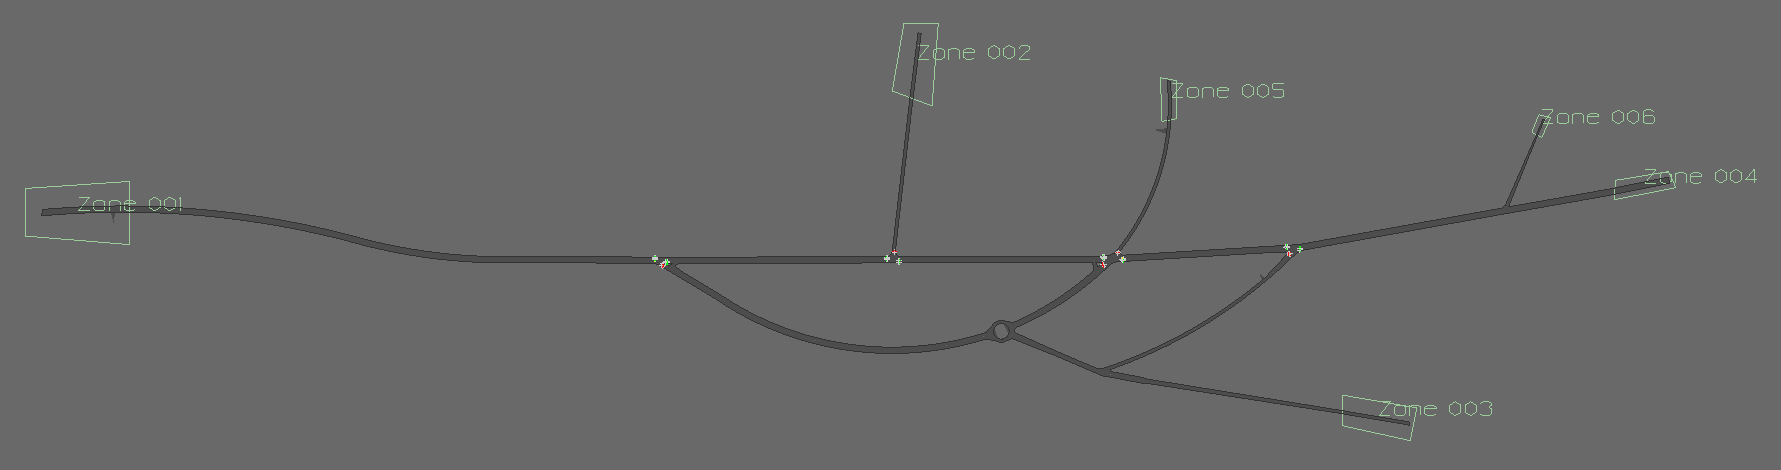
\includegraphics[width=\linewidth]{figuras/network8.png}
    \caption{Red de transporte utilizada para las pruebas preliminares.}
    \label{fig:network8}
\end{figure}

La validación preliminar del \emph{framework} se realizó utilizando la implementación de TraCI en Python incluída en la distribución de SUMO. Esta consiste en una librería para Python 2.7+ y 3.0+, la cual implementa un cliente TraCI en su totalidad (\autocite{pytraci, pytracisrc}), permitiendo así la validación del correcto funcionamiento de los comandos implementados en el \emph{framework} PVeins.

Por otro lado, la red de transporte utilizada para las pruebas corresponde a una red simple, incluida por defecto en la instalación de Paramics. Esta red consiste en un corredor central y conjunto de calles que lo intersectan (ver figura \ref{fig:network8}). El flujo de vehículos en la red es medio-bajo, manteniéndose bajo los 500 vehículos activos en toda la red en cualquier momento dado.

A lo largo del desarrollo de este trabajo, se utilizó la librería anteriormente mencionada, junto con el entorno de \emph{debugging} de Visual Studio y la red de transporte, para probar la correcta implementación de cada funcionalidad que se le agregó al \emph{framework}. Se implementaron simples \emph{scripts} en Python para probar cada una de las funcionalidades desarrolladas; sólo se utilizará uno de éstos como ejemplo a continuación, ya que no es factible ni interesante exponer todas las pruebas realizadas en este documento, dada la gran cantidad de éstas que se efectuaron y el alto grado de similitud que existe entre las mismas.

Además, implementado ya el \emph{framework} en su totalidad, se realizaron pruebas de validación de mayor envergadura, midiendo la eficiencia y la efectividad del sistema para la simulación de grandes redes de transporte. Los resultados de éstas pruebas se presentan en el capítulo \ref{cap:validacion}.

\subsection{Ejemplo de script de prueba: cambio de ruta}

\begin{figure}
    \centering
    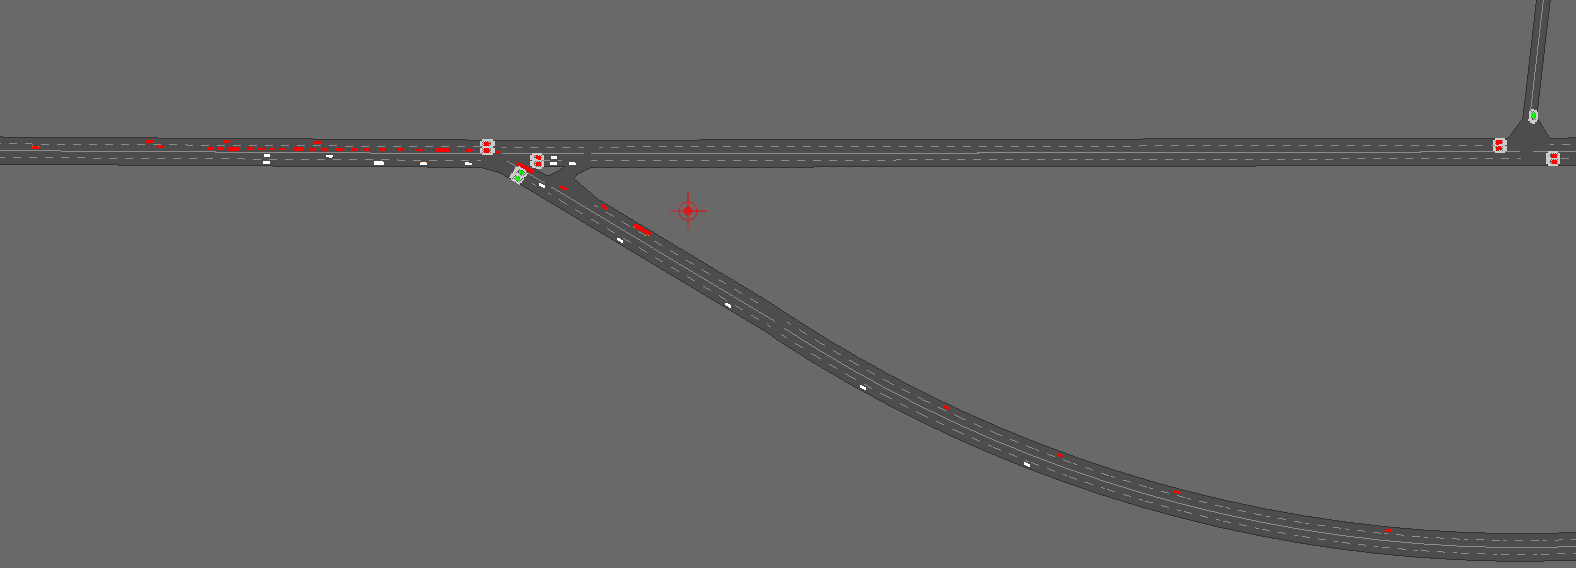
\includegraphics[width=\linewidth]{figuras/network8_routechange.png}
    \caption{Visualización del \emph{test} de cambio de ruta en curso. Los vehículos pintados de rojo son aquellos afectados por el cambio.}
    \label{fig:network8:routechange}
\end{figure}

El código \ref{code:py_routechange} expone el \emph{script} utilizado para una prueba de la funcionalidad del cambio de ruta en TraCI, la cual fue implementada en la última etapa de desarrollo del software por lo que ya se contaba con una base con más funcionalidades sobre la cual construir (\emph{e.g.}, obtención de valores mediante suscripciones).

El procedimiento es simple; el \emph{script} avanza la simulación en un \emph{loop}, obteniendo luego de cada iteración la lista de vehículos en la red. De estos vehículos, encuentra aquellos que se encuentran en la primera calle de una ruta predefinida y procede a cambiar su ruta original por una nueva, al mismo tiempo pintándolos de un color rojo para poder distinguirlos del resto. El resultado puede observarse en la figura \ref{fig:network8:routechange}.

Este código expone de manera clara la estructura del \emph{loop} de simulación TraCI, estructura que se replica en VEINS (aunque de manera mucho más compleja); el cliente es quien controla la ejecución de los pasos de simulación, avanzando el escenario a medida que va realizando sus propios cálculos y análisis. También demuestra las razones por la cual se llevó a cabo el desarrollo en etapas comentado en la sección \ref{sec:metodologia} -- si bien el enfoque de esta prueba es la funcionalidad de cambio de ruta, es necesario también el uso de otras funcionalidades de TraCI como el \emph{handshake} de inicio de conexión (\texttt{traci.init(\dots)}), la suscripción a variables de vehículo (\texttt{traci.vehicle.subscribe(\dots)} y \texttt{.getSubscriptionResults(\dots)}), el avance de la simulación (\texttt{traci.simulationStep()}) y la obtención de variables de vehículo (\texttt{traci.getRoadID(\dots)}).

\begin{figure*}
    \begin{minipage}{\linewidth}
        \lstinputlisting[style=MyPython, caption={\emph{Script} para la prueba de cambio de ruta.}, label={code:py_routechange}]{codigo/pytraci_routechange.py}
    \end{minipage}
\end{figure*}



\chapter{Validación}\label{cap:validacion}

La implementación del \emph{plugin} se sometió a un conjunto de diversas pruebas para verificar su correcto funcionamiento y la eficiencia del \emph{framework}. Estas pruebas consistieron en la simulación de escenarios realistas, de idéntica complejidad a aquellos escenarios para los que fue concebido y diseñado. 

\minitoc

\section{Escenario y Análisis}\label{sec:experiments}
\subsection{Escenario modelado}

\begin{figure}[tpb]
    \centering
    \begin{subfigure}{0.8\textwidth}
        \centering
        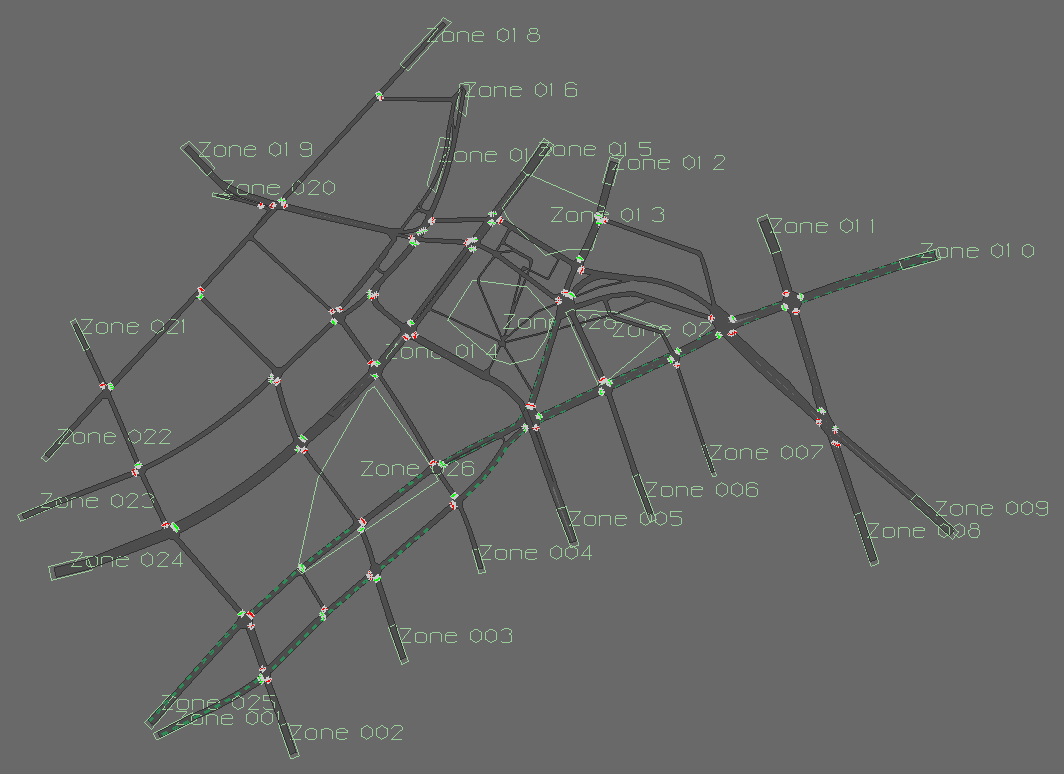
\includegraphics[width=\linewidth]{figuras/costanera.png}
        \caption{Mapa en Paramics del escenario simulado.}
    \end{subfigure}\\
    \begin{subfigure}{0.8\textwidth}
        \centering
        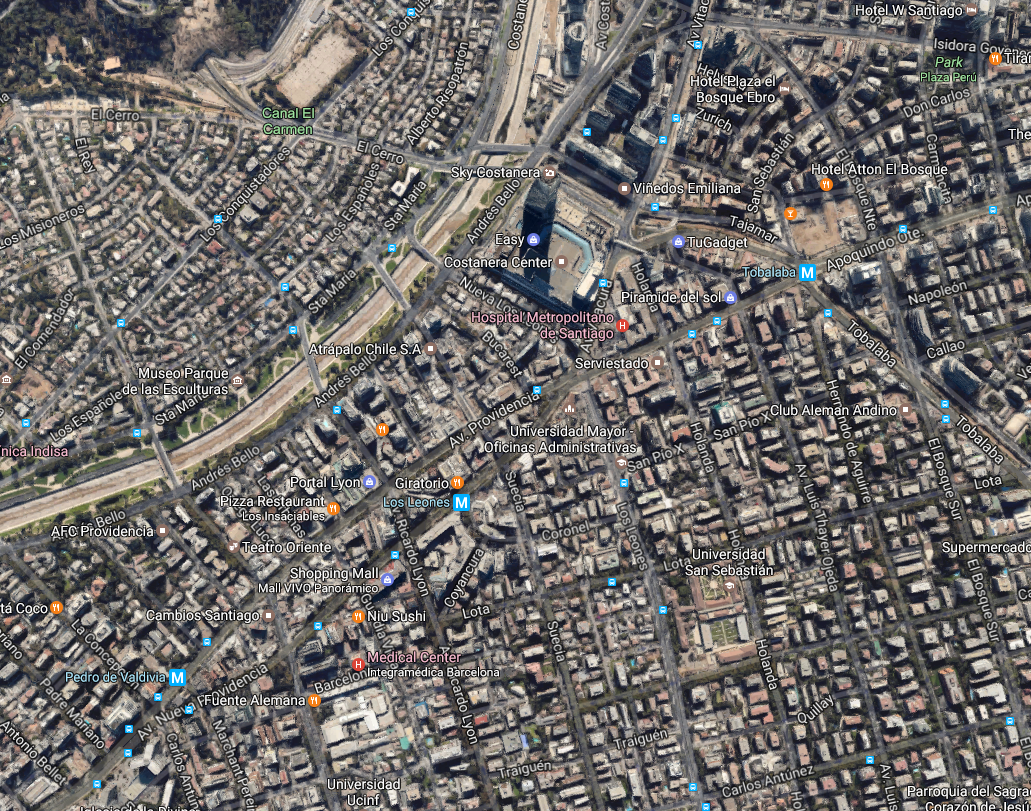
\includegraphics[width=\linewidth]{figuras/costanera_maps.png}
        \caption{Escenario simulado en la ``vida real'', Google Maps.}
    \end{subfigure}
    \caption{Escenario modelado, Paramics vs. ``vida real''.}
    \label{fig:costanera}
\end{figure}

Como escenario de transporte para la validación del \emph{framework} se utilizó un modelo de un sector de la ciudad de Santiago de Chile, el cual consiste en una simulación detallada del flujo vehicular en la comuna de Providencia. Este modelo fue creado en 2010 por Víctor Zúñiga para el desarrollo de su memoria de grado \autocite{zuniga}, y simula el impacto sobre el sector entre las avenidas Providencia, Tobalaba, Andrés Bello y Santa María proyectado en ese entonces por la construcción de un nuevo centro comercial (ver figura \ref{fig:costanera}).

Sobre este escenario vehicular se construyó un modelo de ITS, utilizando el \emph{plugin} desarrollado y el \emph{framework} VEINS en OMNeT++. Este consistió en un escenario en que un vehículo sufre un desperfecto en una cierta calle de la simulación y emite \emph{beacons} de advertencia en \emph{broadcast} a todos los demás vehículos que se encuentran dentro del alcance de la transmisión. A aquellos vehículos que reciben un \emph{beacon}, y que se puede predecir ingresarán a la calle en que se encuentra el vehículo averiado, se les modifica luego su ruta mediante VEINS y TraCI.

De manera más detallada, el escenario funciona de la siguiente manera:

\begin{enumerate}
    \item Al iniciarse el \emph{framework}, OMNeT++ (utilizando VEINS) inicializa una conexión TraCI con el \emph{plugin} en Paramics.
    \item Por cada vehículo que ingresa a la red de transporte, OMNeT++ crea un módulo dotado de lógica y capacidades comunicaciones en su simulación de red, y asocia el movimiento de este módulo al vehículo en Paramics. En adelante, se entenderá por ``vehículo'' el par consistente en el vehículo en Paramics y su módulo asociado en OMNeT++.
    \item Periódicamente se verifica la posición de cada vehículo, y al detectar el primero en ingresar a la calle del ``accidente'', este es detenido. La calle en cuestión para esta simulación fue el arco ``40:5'', el cual corresponde a Avenida Vitacura, frente al centro comercial. El vehículo además se colorea rojo para su fácil identificación.
    \item El módulo OMNeT++ del vehículo accidentado emite luego, cada 5 segundos, un mensaje WAVE \autocite{80211wave} en \emph{broadcast}.
    \item Aquellos vehículos que reciban el \emph{beacon} de emergencia, se encuentren en alguna de las calles aledañas al accidente y que tengan un destino que probablemente los haga pasar por la calle afectada, cambian su ruta a utilizar el arco ``40:7'', correspondiente a la calle Holanda, entre Avda. Vitacura y Avda. Providencia. Además, se cambia su color a púrpura para visualizarlos de manera más fácil en Paramics.
\end{enumerate}

Esta simulación dura un total de \textbf{15 minutos de tiempo \emph{simulado}}, y se ejecutó con múltiples configuraciones del sistema de transporte y del sistema de comunicaciones, las cuales se verán a continuación en las secciones \ref{sec:results:performance} y \ref{sec:results:vehicular}. Las especificaciones técnicas del equipo en donde se realizaron estos experimentos pueden observarse en la tabla \ref{table:systemspecs}.

\begin{table}[tpb]
    \centering
    \begin{tabular}{@{}ll@{}}
        \toprule
        Sistema Operativo     & Windows 10 v.10.0.14393         \\
        Procesador            & Intel Core i7 4720HQ @ 2.60 GHz \\
        N$^{o}$ de Núcleos / Threads & 4 núcleos / 8 threads\\
        Arquitectura          & x86\_64                         \\
        RAM                   & 12 GB DDR3L 1600 MHz            \\
        Tarjeta de Video      & NVIDIA GeForce GTX 960M         \\
        Memoria Video         & 2 GB GDDR5                      \\ \bottomrule
    \end{tabular}
    \caption{Especificaciones técnicas del entorno de simulación.}
    \label{table:systemspecs}
\end{table}

Las mediciones realizadas se enfocaron a probar el funcionamiento del \emph{framework} en dos categorías de análisis; \textbf{eficiencia computacional} de la implementación e \textbf{impacto sobre el modelo de transporte}. De esta manera se pretende demostrar que PVEINS es una opción viable para la investigación en Sistemas Inteligentes de Transporte, tanto en términos de los recursos que utiliza el \emph{framework} para la ejecución de las simulaciones como en términos de la validez de los resultados obtenidos.

Los resultados obtenidos de cada simulación fuero exportados desde OMNeT++ a archivos CSV, los cuales luego se analizaron utilizando Python 3.6.
Se utilizaron las librerías Pandas \autocite{pandas}, para el manejo de los datos de manera eficiente, Numpy \autocite{numpy}, para cálculos, y Matplotlib \autocite{matplotlib} y matplotlib2tikz \autocite{matplotlib2tikz} para la generación de gráficos que permitiesen analizar los datos de manera más efectiva e intuitiva.


\section{Eficiencia Computacional}\label{sec:results:performance}
\subsection{Mediciones Realizadas}

El principal factor a medir en esta categoría es la relación entre la cantidad de vehículos en una simulación y el tiempo real que demora el \emph{framework} en simular el escenario, para una duración en tiempo simulado específica. De esta manera, se pretende caracterizar el comportamiento del \emph{software} para escenarios vehiculares de alta complejidad, en los cuales pueden llegar a interactuar miles de vehículos. Además, interesa también la carga en términos de recursos de sistema que genera la ejecución de la simulación sobre el equipo de prueba. 

A través de éstos datos se pretende generar un perfil del \emph{software} que indique los requisitos que impone sobre el entorno de simulación, y su factibilidad de uso para sistemas de transporte complejos tanto en entornos de simulación de alto rendimiento como de mediano y bajo.

Antes de detallar las simulaciones realizadas, se debe definir el término \emph{factor de demanda}. Éste corresponde a un elemento de configuración de la simulación de transporte en Paramics, el cual caracteriza la carga vehicular sobre el sistema de transporte en cada instante de tiempo. En términos más simples, el factor de demanda regula la cantidad de vehículos que Paramics inserta a la red durante la simulación; es un valor porcentual cuya correspondencia en cantidad real de vehículos en la red dependerá de las características particulares de cada simulación. Sin embargo, los valores aproximados para el escenario utilizado, para distintos factores de demanda, pueden observarse en la tabla \ref{table:demandfactor}.

\begin{table}[tpb]
    \centering
    \begin{tabular}{@{}rrr@{}}
        \textbf{Factor de Demanda} & \textbf{Ctdad. Prom. Vehículos} \\ \midrule
        100\%           & 1379.9 \\ %\midrule
        75\%            & 868.75 \\ %\midrule
        50\%            & 514.5825 \\ %\midrule
        25\%            & 246.5675 \\ \bottomrule
    \end{tabular}
    \caption[Factor de demanda vs. cantidad promedio de vehículos]{Tabla de relación entre factor de demanda y cantidad promedio de vehículos por instante de tiempo en el escenario de prueba.}
    \label{table:demandfactor}
\end{table}

Se realizaron entonces 16 ejecuciones del escenario (de aquí en adelante, denominadas \emph{runs}) con cuatro factores de demanda distintos (4 \emph{runs} con 100\%, 4 con 75\%, 4 con 50\% y 4 con 25\%) y cada una con una \emph{semilla} distinta para los generadores de números pseudoaleatorios. De éstos \emph{runs} se extrajeron las siguientes estadísticas:

\begin{enumerate}
    \item Timestamp de inicio del \emph{run}.
    \item Timestamp de fin del \emph{run}.
    \item Duración en tiempo real del \emph{run}.
    \item Cantidad de vehículos en la red de transporte, cada 1 minuto de tiempo simulado.
\end{enumerate}

De manera adicional, para determinar el principal origen del \emph{overhead} presente en las simulaciones, se ejecutaron también una serie de \emph{runs} de la simulación \emph{sin} OMNeT++, sólamente utilizando el \emph{plugin} controlado por un \emph{script} Python, y se midió su tiempo de ejecución.

Finalmente, se realizó una ejecución adicional de un \emph{run} con factor de demanda 100\%, y se midió la carga sobre el equipo de prueba mientras se ejecutaba la simulación utilizando las herramientas de monitoreo de sistema de Microsoft Windows. En específico, se midió la carga porcentual sobre el procesador, la memoria RAM utilizada y la cantidad de operaciones de escritura y lectura del disco físico durante la simulación.

\subsection{Resultados}

\subsubsection{Duración de la Simulación}

La tabla \ref{table:vehiclesvstime} presenta los resultados obtenidos del tiempo de duración de la simulación versus la cantidad de vehículos promedio por instante de tiempo; estos datos se visualizan además de manera gráfica en la figura \ref{fig:vehiclesvstime}.

De estos resultados se puede concluir que el \emph{framework}, como era de esperarse dada la naturaleza de la simulación, presenta una relación levemente exponencial entre la cantidad promedio de nodos en la red vehicular con el tiempo que efectivamente demora una simulación en completar su ejecución.

Se utilizó numpy para calcular un ajuste polinomial a los datos obtenidos, obteniendo la siguiente relación entre cantidad de vehículos promedio en la simulación $N_{v}$ y tiempo de ejecución de ésta en segundos, $T(N_{v})$:

\[ T(N_{v}) = (5.829 \times 10^{-4})N_{v}^{2} + (2.586 \times 10^{-1})N_{v} + 6.317 \]

Esto indica que a pesar de ser exponencial, la relación presenta una curva bastante suavizada. Es factible entonces simular escenarios de escala aún mayor que la presentada en esta memoria (la cual, cabe notar, no es menor), sin mayores dificultades.

La figura \ref{fig:timevsvehicles_evolution} presenta por lo otro lado la evolución de la red vehicular en términos de cantidad de vehículos para un \emph{run} con factor de demanda de 100\%, tanto en tiempo real como en tiempo simulado. Este gráfico permite visualizar además como la cantidad de vehículos en la red afecta el tiempo de ejecución de cada paso de simulación.

Por otro lado, para determinar si la mayor parte del \emph{overhead} en la ejecución de las simulaciones provenía desde el \emph{plugin} en sí o desde OMNeT++, se realizaron 6 \emph{runs} de la simulación, con factor de demanda 100\%, omitiendo la integración con VEINS. Es decir, se ejecutó el escenario dentro de Paramics, con el \emph{plugin} activado, pero sin accidente y sin comunicación entre los nodos, controlado por un \emph{script} Python. Estas mediciones arrojaron como promedio 63.37 segundos de tiempo real por 15 minutos de tiempo simulado, indicando claramente que la mayor parte del \emph{overhead} proviene de OMNeT++, y de la simulación de la comunicación inalámbrica.

\begin{table}[tpb]
    \centering
    \begin{tabular}{@{}rrr@{}}
        \textbf{Factor de Demanda} & \textbf{Nro. Prom. Vehículos} & \textbf{Tiempo Promedio [s]} \\ \midrule
        100\%           & 1379.9          & 1471.5              \\ %\midrule
        75\%            & 868.75          & 683.5               \\ %\midrule
        50\%            & 514.5825        & 275.75              \\ %\midrule
        25\%            & 246.5675        & 113.25              \\ \bottomrule
    \end{tabular}
    \caption[Cantidad de vehículos vs. tiempo real de simulación]{Promedio cantidad de vehículos en simulación (por instante de tiempo) vs. tiempo promedio de simulación, 15 minutos de tiempo simulado.}
    \label{table:vehiclesvstime}
\end{table}

\begin{figure}[htpb]
    \centering    
    % This file was created by matplotlib2tikz v0.6.10.
\begin{tikzpicture}

\definecolor{color0}{rgb}{0.941176470588235,0.392156862745098,0.286274509803922}
\definecolor{color1}{rgb}{0.0901960784313725,0.745098039215686,0.733333333333333}
\definecolor{color2}{rgb}{0.937254901960784,0.176470588235294,0.337254901960784}
\definecolor{color3}{rgb}{0.549019607843137,0.847058823529412,0.403921568627451}
\definecolor{color4}{rgb}{0.184313725490196,0.141176470588235,0.227450980392157}

\begin{axis}[
xlabel={Cantidad promedio veh\'iculos en simulaci\'on},
ylabel={Tiempo $[s]$},
xmin=150, xmax=1490,
ymin=0, ymax=1713,
width=\figurewidth,
height=\figureheight,
tick align=outside,
tick pos=left,
xmajorgrids,
x grid style={lightgray!84.183006535947712!black},
ymajorgrids,
y grid style={lightgray!84.183006535947712!black},
axis line style={black},
xticklabel style={rotate=45},
legend style={at={(0.03,0.97)}, anchor=north west, draw=white!80.0!black, fill=white!89.803921568627459!black},
legend cell align={left},
legend entries={{Ajuste polinomial},{Factor de demanda 100\%},{Factor de demanda 75\%},{Factor de demanda 50\%},{Factor de demanda 25\%}}
]
\addplot [semithick, color0, opacity=0.3, dash pattern=on 1pt off 3pt on 3pt off 3pt]
table {%
0 6.3172112993997
1 6.57640934437459
2 6.83677322746044
3 7.09830294865727
4 7.36099850796506
5 7.62485990538382
6 7.88988714091354
7 8.15608021455424
8 8.4234391263059
9 8.69196387616853
10 8.96165446414212
11 9.23251089022668
12 9.50453315442222
13 9.77772125672872
14 10.0520751971462
15 10.3275949756746
16 10.604280592314
17 10.8821320470644
18 11.1611493399257
19 11.441332470898
20 11.7226814399813
21 12.0051962471755
22 12.2888768924808
23 12.5737233758969
24 12.8597356974241
25 13.1469138570622
26 13.4352578548113
27 13.7247676906713
28 14.0154433646423
29 14.3072848767243
30 14.6002922269173
31 14.8944654152212
32 15.1898044416361
33 15.4863093061619
34 15.7839800087987
35 16.0828165495465
36 16.3828189284053
37 16.683987145375
38 16.9863212004557
39 17.2898210936474
40 17.59448682495
41 17.9003183943636
42 18.2073158018881
43 18.5154790475237
44 18.8248081312702
45 19.1353030531276
46 19.4469638130961
47 19.7597904111755
48 20.0737828473658
49 20.3889411216672
50 20.7052652340795
51 21.0227551846028
52 21.341410973237
53 21.6612325999822
54 21.9822200648384
55 22.3043733678055
56 22.6276925088836
57 22.9521774880727
58 23.2778283053727
59 23.6046449607838
60 23.9326274543057
61 24.2617757859387
62 24.5920899556826
63 24.9235699635375
64 25.2562158095033
65 25.5900274935802
66 25.9250050157679
67 26.2611483760667
68 26.5984575744764
69 26.9369326109971
70 27.2765734856288
71 27.6173801983714
72 27.959352749225
73 28.3024911381895
74 28.6467953652651
75 28.9922654304516
76 29.338901333749
77 29.6867030751575
78 30.0356706546769
79 30.3858040723072
80 30.7371033280486
81 31.0895684219009
82 31.4431993538641
83 31.7979961239384
84 32.1539587321236
85 32.5110871784197
86 32.8693814628269
87 33.228841585345
88 33.5894675459741
89 33.9512593447141
90 34.3142169815651
91 34.6783404565271
92 35.0436297696
93 35.410084920784
94 35.7777059100788
95 36.1464927374847
96 36.5164454030015
97 36.8875639066293
98 37.259848248368
99 37.6332984282178
100 38.0079144461785
101 38.3836963022501
102 38.7606439964327
103 39.1387575287263
104 39.5180368991309
105 39.8984821076464
106 40.2800931542729
107 40.6628700390104
108 41.0468127618588
109 41.4319213228182
110 41.8181957218886
111 42.2056359590699
112 42.5942420343622
113 42.9840139477655
114 43.3749516992797
115 43.7670552889049
116 44.1603247166411
117 44.5547599824882
118 44.9503610864463
119 45.3471280285154
120 45.7450608086954
121 46.1441594269864
122 46.5444238833884
123 46.9458541779013
124 47.3484503105253
125 47.7522122812601
126 48.157140090106
127 48.5632337370628
128 48.9704932221306
129 49.3789185453093
130 49.7885097065991
131 50.1992667059997
132 50.6111895435114
133 51.024278219134
134 51.4385327328676
135 51.8539530847122
136 52.2705392746677
137 52.6882913027342
138 53.1072091689116
139 53.5272928732001
140 53.9485424155995
141 54.3709577961098
142 54.7945390147311
143 55.2192860714635
144 55.6451989663067
145 56.0722776992609
146 56.5005222703261
147 56.9299326795023
148 57.3605089267894
149 57.7922510121876
150 58.2251589356966
151 58.6592326973167
152 59.0944722970477
153 59.5308777348896
154 59.9684490108426
155 60.4071861249065
156 60.8470890770814
157 61.2881578673672
158 61.730392495764
159 62.1737929622718
160 62.6183592668906
161 63.0640914096203
162 63.510989390461
163 63.9590532094126
164 64.4082828664752
165 64.8586783616488
166 65.3102396949334
167 65.7629668663289
168 66.2168598758354
169 66.6719187234528
170 67.1281434091813
171 67.5855339330207
172 68.044090294971
173 68.5038124950323
174 68.9647005332046
175 69.4267544094879
176 69.8899741238822
177 70.3543596763873
178 70.8199110670035
179 71.2866282957306
180 71.7545113625687
181 72.2235602675178
182 72.6937750105779
183 73.1651555917489
184 73.6377020110308
185 74.1114142684238
186 74.5862923639277
187 75.0623362975426
188 75.5395460692684
189 76.0179216791052
190 76.497463127053
191 76.9781704131117
192 77.4600435372815
193 77.9430824995621
194 78.4272872999538
195 78.9126579384564
196 79.39919441507
197 79.8868967297945
198 80.3757648826301
199 80.8657988735766
200 81.356998702634
201 81.8493643698024
202 82.3428958750818
203 82.8375932184722
204 83.3334563999735
205 83.8304854195858
206 84.3286802773091
207 84.8280409731433
208 85.3285675070885
209 85.8302598791446
210 86.3331180893118
211 86.8371421375899
212 87.3423320239789
213 87.848687748479
214 88.35620931109
215 88.864896711812
216 89.3747499506449
217 89.8857690275888
218 90.3979539426437
219 90.9113046958095
220 91.4258212870863
221 91.9415037164741
222 92.4583519839728
223 92.9763660895826
224 93.4955460333032
225 94.0158918151349
226 94.5374034350775
227 95.0600808931311
228 95.5839241892956
229 96.1089333235712
230 96.6351082959576
231 97.1624491064551
232 97.6909557550635
233 98.2206282417829
234 98.7514665666133
235 99.2834707295546
236 99.8166407306069
237 100.35097656977
238 100.886478247044
239 101.42314576243
240 101.960979115926
241 102.499978307533
242 103.040143337251
243 103.58147420508
244 104.12397091102
245 104.667633455071
246 105.212461837233
247 105.758456057506
248 106.30561611589
249 106.853942012385
250 107.403433746991
251 107.954091319707
252 108.505914730535
253 109.058903979474
254 109.613059066524
255 110.168379991684
256 110.724866754956
257 111.282519356339
258 111.841337795832
259 112.401322073437
260 112.962472189152
261 113.524788142979
262 114.088269934916
263 114.652917564965
264 115.218731033124
265 115.785710339394
266 116.353855483776
267 116.923166466268
268 117.493643286871
269 118.065285945585
270 118.638094442411
271 119.212068777347
272 119.787208950394
273 120.363514961552
274 120.940986810821
275 121.519624498201
276 122.099428023692
277 122.680397387294
278 123.262532589007
279 123.845833628831
280 124.430300506766
281 125.015933222812
282 125.602731776968
283 126.190696169236
284 126.779826399615
285 127.370122468105
286 127.961584374705
287 128.554212119417
288 129.14800570224
289 129.742965123173
290 130.339090382218
291 130.936381479373
292 131.53483841464
293 132.134461188017
294 132.735249799505
295 133.337204249105
296 133.940324536815
297 134.544610662637
298 135.150062626569
299 135.756680428612
300 136.364464068766
301 136.973413547032
302 137.583528863408
303 138.194810017895
304 138.807257010493
305 139.420869841202
306 140.035648510022
307 140.651593016953
308 141.268703361995
309 141.886979545148
310 142.506421566412
311 143.127029425787
312 143.748803123272
313 144.371742658869
314 144.995848032577
315 145.621119244396
316 146.247556294326
317 146.875159182366
318 147.503927908518
319 148.13386247278
320 148.764962875154
321 149.397229115639
322 150.030661194234
323 150.665259110941
324 151.301022865758
325 151.937952458686
326 152.576047889726
327 153.215309158876
328 153.855736266137
329 154.49732921151
330 155.140087994993
331 155.784012616587
332 156.429103076292
333 157.075359374109
334 157.722781510036
335 158.371369484074
336 159.021123296223
337 159.672042946483
338 160.324128434854
339 160.977379761336
340 161.631796925929
341 162.287379928633
342 162.944128769448
343 163.602043448373
344 164.26112396541
345 164.921370320558
346 165.582782513817
347 166.245360545186
348 166.909104414667
349 167.574014122259
350 168.240089667961
351 168.907331051775
352 169.575738273699
353 170.245311333735
354 170.916050231881
355 171.587954968139
356 172.261025542507
357 172.935261954987
358 173.610664205577
359 174.287232294278
360 174.964966221091
361 175.643865986014
362 176.323931589048
363 177.005163030193
364 177.687560309449
365 178.371123426817
366 179.055852382295
367 179.741747175884
368 180.428807807584
369 181.117034277395
370 181.806426585317
371 182.49698473135
372 183.188708715494
373 183.881598537748
374 184.575654198114
375 185.270875696591
376 185.967263033179
377 186.664816207877
378 187.363535220687
379 188.063420071608
380 188.764470760639
381 189.466687287782
382 190.170069653036
383 190.8746178564
384 191.580331897876
385 192.287211777462
386 192.99525749516
387 193.704469050968
388 194.414846444887
389 195.126389676918
390 195.839098747059
391 196.552973655311
392 197.268014401675
393 197.984220986149
394 198.701593408734
395 199.42013166943
396 200.139835768237
397 200.860705705155
398 201.582741480184
399 202.305943093324
400 203.030310544575
401 203.755843833937
402 204.48254296141
403 205.210407926994
404 205.939438730689
405 206.669635372495
406 207.400997852412
407 208.133526170439
408 208.867220326578
409 209.602080320828
410 210.338106153189
411 211.07529782366
412 211.813655332243
413 212.553178678936
414 213.293867863741
415 214.035722886656
416 214.778743747683
417 215.52293044682
418 216.268282984069
419 217.014801359428
420 217.762485572898
421 218.51133562448
422 219.261351514172
423 220.012533241975
424 220.76488080789
425 221.518394211915
426 222.273073454051
427 223.028918534298
428 223.785929452656
429 224.544106209125
430 225.303448803705
431 226.063957236396
432 226.825631507198
433 227.588471616111
434 228.352477563135
435 229.11764934827
436 229.883986971516
437 230.651490432872
438 231.42015973234
439 232.189994869919
440 232.960995845609
441 233.733162659409
442 234.506495311321
443 235.280993801343
444 236.056658129477
445 236.833488295722
446 237.611484300077
447 238.390646142544
448 239.170973823121
449 239.952467341809
450 240.735126698609
451 241.518951893519
452 242.30394292654
453 243.090099797673
454 243.877422506916
455 244.66591105427
456 245.455565439735
457 246.246385663312
458 247.038371724999
459 247.831523624797
460 248.625841362706
461 249.421324938726
462 250.217974352857
463 251.015789605099
464 251.814770695452
465 252.614917623916
466 253.41623039049
467 254.218708995176
468 255.022353437973
469 255.827163718881
470 256.6331398379
471 257.440281795029
472 258.24858959027
473 259.058063223622
474 259.868702695084
475 260.680508004658
476 261.493479152342
477 262.307616138138
478 263.122918962044
479 263.939387624062
480 264.75702212419
481 265.575822462429
482 266.39578863878
483 267.216920653241
484 268.039218505813
485 268.862682196497
486 269.687311725291
487 270.513107092196
488 271.340068297212
489 272.168195340339
490 272.997488221577
491 273.827946940926
492 274.659571498386
493 275.492361893957
494 276.326318127639
495 277.161440199432
496 277.997728109336
497 278.835181857351
498 279.673801443477
499 280.513586867714
500 281.354538130061
501 282.19665523052
502 283.03993816909
503 283.88438694577
504 284.730001560562
505 285.576782013465
506 286.424728304478
507 287.273840433603
508 288.124118400838
509 288.975562206185
510 289.828171849642
511 290.681947331211
512 291.53688865089
513 292.39299580868
514 293.250268804582
515 294.108707638594
516 294.968312310717
517 295.829082820951
518 296.691019169297
519 297.554121355753
520 298.41838938032
521 299.283823242998
522 300.150422943787
523 301.018188482687
524 301.887119859698
525 302.75721707482
526 303.628480128053
527 304.500909019397
528 305.374503748852
529 306.249264316417
530 307.125190722094
531 308.002282965882
532 308.880541047781
533 309.75996496779
534 310.640554725911
535 311.522310322143
536 312.405231756485
537 313.289319028939
538 314.174572139503
539 315.060991088179
540 315.948575874965
541 316.837326499863
542 317.727242962871
543 318.618325263991
544 319.510573403221
545 320.403987380562
546 321.298567196014
547 322.194312849578
548 323.091224341252
549 323.989301671037
550 324.888544838933
551 325.78895384494
552 326.690528689058
553 327.593269371287
554 328.497175891627
555 329.402248250078
556 330.30848644664
557 331.215890481313
558 332.124460354097
559 333.034196064992
560 333.945097613998
561 334.857165001115
562 335.770398226342
563 336.684797289681
564 337.600362191131
565 338.517092930691
566 339.434989508363
567 340.354051924146
568 341.274280178039
569 342.195674270044
570 343.118234200159
571 344.041959968386
572 344.966851574723
573 345.892909019171
574 346.820132301731
575 347.748521422401
576 348.678076381182
577 349.608797178075
578 350.540683813078
579 351.473736286192
580 352.407954597417
581 353.343338746753
582 354.279888734201
583 355.217604559759
584 356.156486223428
585 357.096533725208
586 358.037747065099
587 358.980126243101
588 359.923671259214
589 360.868382113438
590 361.814258805772
591 362.761301336218
592 363.709509704775
593 364.658883911443
594 365.609423956221
595 366.561129839111
596 367.514001560112
597 368.468039119223
598 369.423242516446
599 370.37961175178
600 371.337146825224
601 372.29584773678
602 373.255714486446
603 374.216747074223
604 375.178945500112
605 376.142309764111
606 377.106839866222
607 378.072535806443
608 379.039397584775
609 380.007425201218
610 380.976618655773
611 381.946977948438
612 382.918503079214
613 383.891194048101
614 384.865050855099
615 385.840073500208
616 386.816261983428
617 387.793616304759
618 388.772136464201
619 389.751822461754
620 390.732674297418
621 391.714691971193
622 392.697875483079
623 393.682224833075
624 394.667740021183
625 395.654421047402
626 396.642267911731
627 397.631280614172
628 398.621459154724
629 399.612803533386
630 400.60531375016
631 401.598989805044
632 402.59383169804
633 403.589839429146
634 404.587012998364
635 405.585352405692
636 406.584857651132
637 407.585528734682
638 408.587365656343
639 409.590368416115
640 410.594537013999
641 411.599871449993
642 412.606371724098
643 413.614037836314
644 414.622869786641
645 415.632867575079
646 416.644031201628
647 417.656360666288
648 418.669855969059
649 419.684517109941
650 420.700344088934
651 421.717336906038
652 422.735495561253
653 423.754820054579
654 424.775310386016
655 425.796966555563
656 426.819788563222
657 427.843776408992
658 428.868930092872
659 429.895249614864
660 430.922734974967
661 431.95138617318
662 432.981203209505
663 434.01218608394
664 435.044334796487
665 436.077649347144
666 437.112129735913
667 438.147775962792
668 439.184588027782
669 440.222565930883
670 441.261709672096
671 442.302019251419
672 443.343494668853
673 444.386135924398
674 445.429943018054
675 446.474915949821
676 447.5210547197
677 448.568359327689
678 449.616829773789
679 450.666466058
680 451.717268180322
681 452.769236140755
682 453.822369939298
683 454.876669575953
684 455.932135050719
685 456.988766363596
686 458.046563514583
687 459.105526503682
688 460.165655330892
689 461.226949996213
690 462.289410499644
691 463.353036841187
692 464.41782902084
693 465.483787038605
694 466.55091089448
695 467.619200588467
696 468.688656120564
697 469.759277490773
698 470.831064699092
699 471.904017745522
700 472.978136630064
701 474.053421352716
702 475.129871913479
703 476.207488312353
704 477.286270549338
705 478.366218624435
706 479.447332537642
707 480.52961228896
708 481.613057878389
709 482.697669305929
710 483.78344657158
711 484.870389675342
712 485.958498617215
713 487.047773397199
714 488.138214015293
715 489.229820471499
716 490.322592765816
717 491.416530898244
718 492.511634868782
719 493.607904677432
720 494.705340324193
721 495.803941809064
722 496.903709132047
723 498.00464229314
724 499.106741292345
725 500.210006129661
726 501.314436805087
727 502.420033318624
728 503.526795670273
729 504.634723860032
730 505.743817887902
731 506.854077753884
732 507.965503457976
733 509.078095000179
734 510.191852380493
735 511.306775598919
736 512.422864655455
737 513.540119550102
738 514.65854028286
739 515.778126853729
740 516.898879262709
741 518.0207975098
742 519.143881595002
743 520.268131518315
744 521.393547279739
745 522.520128879273
746 523.647876316919
747 524.776789592676
748 525.906868706544
749 527.038113658522
750 528.170524448612
751 529.304101076813
752 530.438843543124
753 531.574751847547
754 532.711825990081
755 533.850065970725
756 534.98947178948
757 536.130043446347
758 537.271780941324
759 538.414684274413
760 539.558753445612
761 540.703988454923
762 541.850389302344
763 542.997955987876
764 544.146688511519
765 545.296586873273
766 546.447651073139
767 547.599881111115
768 548.753276987202
769 549.9078387014
770 551.063566253709
771 552.220459644129
772 553.37851887266
773 554.537743939302
774 555.698134844055
775 556.859691586919
776 558.022414167894
777 559.186302586979
778 560.351356844176
779 561.517576939484
780 562.684962872902
781 563.853514644432
782 565.023232254073
783 566.194115701824
784 567.366164987687
785 568.539380111661
786 569.713761073745
787 570.889307873941
788 572.066020512247
789 573.243898988664
790 574.422943303193
791 575.603153455832
792 576.784529446582
793 577.967071275444
794 579.150778942416
795 580.335652447499
796 581.521691790693
797 582.708896971999
798 583.897267991415
799 585.086804848942
800 586.27750754458
801 587.469376078329
802 588.662410450189
803 589.85661066016
804 591.051976708242
805 592.248508594435
806 593.446206318739
807 594.645069881153
808 595.845099281679
809 597.046294520316
810 598.248655597064
811 599.452182511922
812 600.656875264892
813 601.862733855973
814 603.069758285164
815 604.277948552467
816 605.48730465788
817 606.697826601405
818 607.90951438304
819 609.122368002787
820 610.336387460644
821 611.551572756613
822 612.767923890692
823 613.985440862882
824 615.204123673184
825 616.423972321596
826 617.644986808119
827 618.867167132753
828 620.090513295498
829 621.315025296355
830 622.540703135322
831 623.7675468124
832 624.995556327589
833 626.224731680889
834 627.4550728723
835 628.686579901822
836 629.919252769455
837 631.153091475198
838 632.388096019053
839 633.624266401019
840 634.861602621096
841 636.100104679284
842 637.339772575582
843 638.580606309992
844 639.822605882513
845 641.065771293144
846 642.310102541887
847 643.55559962874
848 644.802262553705
849 646.05009131678
850 647.299085917967
851 648.549246357264
852 649.800572634673
853 651.053064750192
854 652.306722703822
855 653.561546495564
856 654.817536125416
857 656.074691593379
858 657.333012899453
859 658.592500043638
860 659.853153025934
861 661.114971846342
862 662.37795650486
863 663.642107001489
864 664.907423336229
865 666.17390550908
866 667.441553520042
867 668.710367369114
868 669.980347056298
869 671.251492581593
870 672.523803944999
871 673.797281146516
872 675.071924186143
873 676.347733063882
874 677.624707779732
875 678.902848333693
876 680.182154725764
877 681.462626955947
878 682.74426502424
879 684.027068930645
880 685.31103867516
881 686.596174257787
882 687.882475678524
883 689.169942937372
884 690.458576034332
885 691.748374969402
886 693.039339742583
887 694.331470353876
888 695.624766803279
889 696.919229090793
890 698.214857216418
891 699.511651180154
892 700.809610982001
893 702.108736621959
894 703.409028100028
895 704.710485416208
896 706.0131085705
897 707.316897562901
898 708.621852393414
899 709.927973062038
900 711.235259568773
901 712.543711913619
902 713.853330096576
903 715.164114117643
904 716.476063976822
905 717.789179674112
906 719.103461209512
907 720.418908583024
908 721.735521794647
909 723.05330084438
910 724.372245732225
911 725.69235645818
912 727.013633022246
913 728.336075424424
914 729.659683664712
915 730.984457743112
916 732.310397659622
917 733.637503414243
918 734.965775006975
919 736.295212437819
920 737.625815706773
921 738.957584813838
922 740.290519759014
923 741.624620542301
924 742.959887163699
925 744.296319623208
926 745.633917920828
927 746.972682056559
928 748.312612030401
929 749.653707842354
930 750.995969492418
931 752.339396980593
932 753.683990306879
933 755.029749471275
934 756.376674473783
935 757.724765314402
936 759.074021993131
937 760.424444509972
938 761.776032864924
939 763.128787057986
940 764.48270708916
941 765.837792958444
942 767.19404466584
943 768.551462211346
944 769.910045594964
945 771.269794816692
946 772.630709876531
947 773.992790774482
948 775.356037510543
949 776.720450084715
950 778.086028496998
951 779.452772747392
952 780.820682835898
953 782.189758762514
954 783.560000527241
955 784.931408130079
956 786.303981571028
957 787.677720850088
958 789.052625967259
959 790.428696922541
960 791.805933715934
961 793.184336347437
962 794.563904817052
963 795.944639124778
964 797.326539270615
965 798.709605254563
966 800.093837076621
967 801.479234736791
968 802.865798235072
969 804.253527571463
970 805.642422745966
971 807.032483758579
972 808.423710609304
973 809.816103298139
974 811.209661825086
975 812.604386190143
976 814.000276393312
977 815.397332434591
978 816.795554313981
979 818.194942031483
980 819.595495587095
981 820.997214980818
982 822.400100212652
983 823.804151282597
984 825.209368190653
985 826.615750936821
986 828.023299521099
987 829.432013943488
988 830.841894203988
989 832.252940302598
990 833.66515223932
991 835.078530014153
992 836.493073627097
993 837.908783078152
994 839.325658367318
995 840.743699494594
996 842.162906459982
997 843.583279263481
998 845.004817905091
999 846.427522384811
1000 847.851392702643
1001 849.276428858586
1002 850.702630852639
1003 852.129998684803
1004 853.558532355079
1005 854.988231863465
1006 856.419097209963
1007 857.851128394571
1008 859.284325417291
1009 860.718688278121
1010 862.154216977062
1011 863.590911514114
1012 865.028771889278
1013 866.467798102552
1014 867.907990153937
1015 869.349348043433
1016 870.79187177104
1017 872.235561336758
1018 873.680416740587
1019 875.126437982527
1020 876.573625062578
1021 878.02197798074
1022 879.471496737013
1023 880.922181331397
1024 882.374031763892
1025 883.827048034497
1026 885.281230143214
1027 886.736578090042
1028 888.19309187498
1029 889.65077149803
1030 891.109616959191
1031 892.569628258462
1032 894.030805395845
1033 895.493148371338
1034 896.956657184943
1035 898.421331836659
1036 899.887172326485
1037 901.354178654422
1038 902.822350820471
1039 904.29168882463
1040 905.7621926669
1041 907.233862347282
1042 908.706697865774
1043 910.180699222377
1044 911.655866417091
1045 913.132199449916
1046 914.609698320853
1047 916.0883630299
1048 917.568193577058
1049 919.049189962327
1050 920.531352185707
1051 922.014680247198
1052 923.4991741468
1053 924.984833884512
1054 926.471659460336
1055 927.959650874271
1056 929.448808126317
1057 930.939131216474
1058 932.430620144741
1059 933.92327491112
1060 935.41709551561
1061 936.91208195821
1062 938.408234238922
1063 939.905552357744
1064 941.404036314678
1065 942.903686109722
1066 944.404501742878
1067 945.906483214144
1068 947.409630523522
1069 948.91394367101
1070 950.419422656609
1071 951.92606748032
1072 953.433878142141
1073 954.942854642073
1074 956.452996980116
1075 957.964305156271
1076 959.476779170536
1077 960.990419022912
1078 962.505224713399
1079 964.021196241997
1080 965.538333608706
1081 967.056636813526
1082 968.576105856457
1083 970.096740737499
1084 971.618541456652
1085 973.141508013916
1086 974.66564040929
1087 976.190938642776
1088 977.717402714373
1089 979.245032624081
1090 980.7738283719
1091 982.303789957829
1092 983.83491738187
1093 985.367210644021
1094 986.900669744284
1095 988.435294682658
1096 989.971085459142
1097 991.508042073737
1098 993.046164526444
1099 994.585452817261
1100 996.12590694619
1101 997.667526913229
1102 999.210312718379
1103 1000.75426436164
1104 1002.29938184301
1105 1003.8456651625
1106 1005.39311432009
1107 1006.9417293158
1108 1008.49151014961
1109 1010.04245682154
1110 1011.59456933158
1111 1013.14784767973
1112 1014.70229186599
1113 1016.25790189036
1114 1017.81467775284
1115 1019.37261945343
1116 1020.93172699213
1117 1022.49200036895
1118 1024.05343958388
1119 1025.61604463691
1120 1027.17981552806
1121 1028.74475225732
1122 1030.31085482469
1123 1031.87812323017
1124 1033.44655747376
1125 1035.01615755546
1126 1036.58692347528
1127 1038.1588552332
1128 1039.73195282924
1129 1041.30621626338
1130 1042.88164553564
1131 1044.45824064601
1132 1046.03600159449
1133 1047.61492838108
1134 1049.19502100578
1135 1050.77627946859
1136 1052.35870376952
1137 1053.94229390855
1138 1055.52704988569
1139 1057.11297170095
1140 1058.70005935432
1141 1060.2883128458
1142 1061.87773217538
1143 1063.46831734308
1144 1065.0600683489
1145 1066.65298519282
1146 1068.24706787485
1147 1069.84231639499
1148 1071.43873075325
1149 1073.03631094961
1150 1074.63505698409
1151 1076.23496885668
1152 1077.83604656738
1153 1079.43829011619
1154 1081.04169950311
1155 1082.64627472814
1156 1084.25201579128
1157 1085.85892269254
1158 1087.4669954319
1159 1089.07623400938
1160 1090.68663842496
1161 1092.29820867866
1162 1093.91094477047
1163 1095.52484670039
1164 1097.13991446842
1165 1098.75614807456
1166 1100.37354751881
1167 1101.99211280117
1168 1103.61184392165
1169 1105.23274088023
1170 1106.85480367693
1171 1108.47803231174
1172 1110.10242678466
1173 1111.72798709568
1174 1113.35471324482
1175 1114.98260523208
1176 1116.61166305744
1177 1118.24188672091
1178 1119.87327622249
1179 1121.50583156219
1180 1123.13955273999
1181 1124.77443975591
1182 1126.41049260994
1183 1128.04771130208
1184 1129.68609583233
1185 1131.32564620069
1186 1132.96636240716
1187 1134.60824445174
1188 1136.25129233444
1189 1137.89550605524
1190 1139.54088561416
1191 1141.18743101118
1192 1142.83514224632
1193 1144.48401931957
1194 1146.13406223093
1195 1147.7852709804
1196 1149.43764556798
1197 1151.09118599367
1198 1152.74589225747
1199 1154.40176435939
1200 1156.05880229941
1201 1157.71700607755
1202 1159.3763756938
1203 1161.03691114815
1204 1162.69861244062
1205 1164.3614795712
1206 1166.02551253989
1207 1167.6907113467
1208 1169.35707599161
1209 1171.02460647463
1210 1172.69330279577
1211 1174.36316495501
1212 1176.03419295237
1213 1177.70638678784
1214 1179.37974646142
1215 1181.05427197311
1216 1182.72996332291
1217 1184.40682051082
1218 1186.08484353684
1219 1187.76403240097
1220 1189.44438710322
1221 1191.12590764357
1222 1192.80859402204
1223 1194.49244623862
1224 1196.17746429331
1225 1197.86364818611
1226 1199.55099791702
1227 1201.23951348604
1228 1202.92919489317
1229 1204.62004213841
1230 1206.31205522177
1231 1208.00523414323
1232 1209.69957890281
1233 1211.3950895005
1234 1213.09176593629
1235 1214.7896082102
1236 1216.48861632222
1237 1218.18879027235
1238 1219.8901300606
1239 1221.59263568695
1240 1223.29630715141
1241 1225.00114445399
1242 1226.70714759467
1243 1228.41431657347
1244 1230.12265139038
1245 1231.8321520454
1246 1233.54281853853
1247 1235.25465086977
1248 1236.96764903912
1249 1238.68181304658
1250 1240.39714289215
1251 1242.11363857584
1252 1243.83130009763
1253 1245.55012745754
1254 1247.27012065556
1255 1248.99127969169
1256 1250.71360456593
1257 1252.43709527828
1258 1254.16175182874
1259 1255.88757421731
1260 1257.61456244399
1261 1259.34271650879
1262 1261.07203641169
1263 1262.80252215271
1264 1264.53417373183
1265 1266.26699114907
1266 1268.00097440442
1267 1269.73612349788
1268 1271.47243842945
1269 1273.20991919913
1270 1274.94856580693
1271 1276.68837825283
1272 1278.42935653685
1273 1280.17150065897
1274 1281.91481061921
1275 1283.65928641756
1276 1285.40492805401
1277 1287.15173552858
1278 1288.89970884127
1279 1290.64884799206
1280 1292.39915298096
1281 1294.15062380797
1282 1295.9032604731
1283 1297.65706297633
1284 1299.41203131768
1285 1301.16816549714
1286 1302.9254655147
1287 1304.68393137038
1288 1306.44356306417
1289 1308.20436059608
1290 1309.96632396609
1291 1311.72945317421
1292 1313.49374822045
1293 1315.25920910479
1294 1317.02583582725
1295 1318.79362838781
1296 1320.56258678649
1297 1322.33271102328
1298 1324.10400109818
1299 1325.87645701119
1300 1327.65007876231
1301 1329.42486635155
1302 1331.20081977889
1303 1332.97793904434
1304 1334.75622414791
1305 1336.53567508959
1306 1338.31629186938
1307 1340.09807448727
1308 1341.88102294328
1309 1343.6651372374
1310 1345.45041736964
1311 1347.23686333998
1312 1349.02447514843
1313 1350.813252795
1314 1352.60319627967
1315 1354.39430560246
1316 1356.18658076336
1317 1357.98002176236
1318 1359.77462859948
1319 1361.57040127471
1320 1363.36733978805
1321 1365.16544413951
1322 1366.96471432907
1323 1368.76515035674
1324 1370.56675222253
1325 1372.36951992643
1326 1374.17345346843
1327 1375.97855284855
1328 1377.78481806678
1329 1379.59224912312
1330 1381.40084601757
1331 1383.21060875013
1332 1385.02153732081
1333 1386.83363172959
1334 1388.64689197648
1335 1390.46131806149
1336 1392.27690998461
1337 1394.09366774583
1338 1395.91159134517
1339 1397.73068078262
1340 1399.55093605818
1341 1401.37235717185
1342 1403.19494412364
1343 1405.01869691353
1344 1406.84361554154
1345 1408.66970000765
1346 1410.49695031188
1347 1412.32536645421
1348 1414.15494843466
1349 1415.98569625322
1350 1417.81760990989
1351 1419.65068940467
1352 1421.48493473757
1353 1423.32034590857
1354 1425.15692291768
1355 1426.99466576491
1356 1428.83357445024
1357 1430.67364897369
1358 1432.51488933525
1359 1434.35729553492
1360 1436.2008675727
1361 1438.04560544859
1362 1439.89150916259
1363 1441.7385787147
1364 1443.58681410493
1365 1445.43621533326
1366 1447.28678239971
1367 1449.13851530427
1368 1450.99141404693
1369 1452.84547862771
1370 1454.7007090466
1371 1456.5571053036
1372 1458.41466739871
1373 1460.27339533194
1374 1462.13328910327
1375 1463.99434871271
1376 1465.85657416027
1377 1467.71996544594
1378 1469.58452256971
1379 1471.4502455316
1380 1473.3171343316
1381 1475.18518896971
1382 1477.05440944593
1383 1478.92479576026
1384 1480.79634791271
1385 1482.66906590326
1386 1484.54294973193
1387 1486.4179993987
1388 1488.29421490359
1389 1490.17159624659
1390 1492.0501434277
1391 1493.92985644692
1392 1495.81073530425
1393 1497.69277999969
1394 1499.57599053324
1395 1501.46036690491
1396 1503.34590911468
1397 1505.23261716257
1398 1507.12049104856
1399 1509.00953077267
1400 1510.89973633489
1401 1512.79110773522
1402 1514.68364497366
1403 1516.57734805021
1404 1518.47221696487
1405 1520.36825171765
1406 1522.26545230853
1407 1524.16381873753
1408 1526.06335100463
1409 1527.96404910985
1410 1529.86591305318
1411 1531.76894283462
1412 1533.67313845417
1413 1535.57849991183
1414 1537.4850272076
1415 1539.39272034149
1416 1541.30157931348
1417 1543.21160412359
1418 1545.1227947718
1419 1547.03515125813
1420 1548.94867358257
1421 1550.86336174512
1422 1552.77921574578
1423 1554.69623558455
1424 1556.61442126143
1425 1558.53377277642
1426 1560.45429012953
1427 1562.37597332074
1428 1564.29882235007
1429 1566.2228372175
1430 1568.14801792305
1431 1570.07436446671
1432 1572.00187684848
1433 1573.93055506836
1434 1575.86039912635
1435 1577.79140902245
1436 1579.72358475667
1437 1581.65692632899
1438 1583.59143373943
1439 1585.52710698797
1440 1587.46394607463
1441 1589.4019509994
1442 1591.34112176228
1443 1593.28145836327
1444 1595.22296080237
1445 1597.16562907958
1446 1599.10946319491
1447 1601.05446314834
1448 1603.00062893988
1449 1604.94796056954
1450 1606.89645803731
1451 1608.84612134319
1452 1610.79695048717
1453 1612.74894546927
1454 1614.70210628949
1455 1616.65643294781
1456 1618.61192544424
1457 1620.56858377878
1458 1622.52640795144
1459 1624.4853979622
1460 1626.44555381108
1461 1628.40687549807
1462 1630.36936302317
1463 1632.33301638638
1464 1634.2978355877
1465 1636.26382062713
1466 1638.23097150467
1467 1640.19928822033
1468 1642.16877077409
1469 1644.13941916597
1470 1646.11123339595
1471 1648.08421346405
1472 1650.05835937026
1473 1652.03367111458
1474 1654.01014869701
1475 1655.98779211755
1476 1657.9666013762
1477 1659.94657647296
1478 1661.92771740784
1479 1663.91002418082
1480 1665.89349679192
1481 1667.87813524113
1482 1669.86393952844
1483 1671.85090965387
1484 1673.83904561741
1485 1675.82834741906
1486 1677.81881505883
1487 1679.8104485367
1488 1681.80324785268
1489 1683.79721300678
1490 1685.79234399898
1491 1687.7886408293
1492 1689.78610349773
1493 1691.78473200427
1494 1693.78452634892
1495 1695.78548653168
1496 1697.78761255255
1497 1699.79090441153
1498 1701.79536210862
1499 1703.80098564383
1500 1705.80777501714
1501 1707.81573022857
1502 1709.82485127811
1503 1711.83513816576
1504 1713.84659089152
1505 1715.85920945539
1506 1717.87299385737
1507 1719.88794409746
1508 1721.90406017566
1509 1723.92134209198
1510 1725.9397898464
1511 1727.95940343894
1512 1729.98018286958
1513 1732.00212813834
1514 1734.02523924521
1515 1736.04951619019
1516 1738.07495897328
1517 1740.10156759448
1518 1742.1293420538
1519 1744.15828235122
1520 1746.18838848676
1521 1748.2196604604
1522 1750.25209827216
1523 1752.28570192203
1524 1754.32047141001
1525 1756.35640673609
1526 1758.3935079003
1527 1760.43177490261
1528 1762.47120774303
1529 1764.51180642156
1530 1766.55357093821
1531 1768.59650129296
1532 1770.64059748583
1533 1772.68585951681
1534 1774.73228738589
1535 1776.77988109309
1536 1778.8286406384
1537 1780.87856602183
1538 1782.92965724336
1539 1784.981914303
1540 1787.03533720076
1541 1789.08992593662
1542 1791.1456805106
1543 1793.20260092268
1544 1795.26068717288
1545 1797.31993926119
1546 1799.38035718761
1547 1801.44194095214
1548 1803.50469055478
1549 1805.56860599554
1550 1807.6336872744
1551 1809.69993439137
1552 1811.76734734646
1553 1813.83592613966
1554 1815.90567077096
1555 1817.97658124038
1556 1820.04865754791
1557 1822.12189969355
1558 1824.19630767731
1559 1826.27188149917
1560 1828.34862115914
1561 1830.42652665723
1562 1832.50559799342
1563 1834.58583516773
1564 1836.66723818015
1565 1838.74980703067
1566 1840.83354171931
1567 1842.91844224606
1568 1845.00450861092
1569 1847.0917408139
1570 1849.18013885498
1571 1851.26970273417
1572 1853.36043245148
1573 1855.45232800689
1574 1857.54538940042
1575 1859.63961663206
1576 1861.73500970181
1577 1863.83156860967
1578 1865.92929335564
1579 1868.02818393972
1580 1870.12824036191
1581 1872.22946262222
1582 1874.33185072063
1583 1876.43540465716
1584 1878.5401244318
1585 1880.64601004454
1586 1882.7530614954
1587 1884.86127878437
1588 1886.97066191145
1589 1889.08121087664
1590 1891.19292567995
1591 1893.30580632136
1592 1895.41985280088
1593 1897.53506511852
1594 1899.65144327427
1595 1901.76898726812
1596 1903.88769710009
1597 1906.00757277017
1598 1908.12861427836
1599 1910.25082162466
1600 1912.37419480907
1601 1914.4987338316
1602 1916.62443869223
1603 1918.75130939098
1604 1920.87934592783
1605 1923.0085483028
1606 1925.13891651588
1607 1927.27045056707
1608 1929.40315045637
1609 1931.53701618378
1610 1933.6720477493
1611 1935.80824515293
1612 1937.94560839468
1613 1940.08413747453
1614 1942.2238323925
};
\addplot [semithick, color1, mark=*, mark size=3, mark options={solid}, only marks]
table {%
1398.4 1593
1351.4 1439
1354.67 1388
1415.13 1466
};
\addplot [semithick, color2, mark=*, mark size=3, mark options={solid}, only marks]
table {%
870.2 660
872.27 664
842.13 703
890.4 707
};
\addplot [semithick, color3, mark=*, mark size=3, mark options={solid}, only marks]
table {%
521.13 281
504.4 268
512.2 272
520.6 282
};
\addplot [semithick, color4, mark=*, mark size=3, mark options={solid}, only marks]
table {%
249.67 118
254.8 122
240.87 113
240.93 100
};
\end{axis}

\end{tikzpicture}
    \captionof{figure}[Cantidad de vehículos vs. tiempo real de simulación]{Gráfico de dispersión del promedio de vehículos en simulación por instante de tiempo vs. tiempo total de simulación, para una simulación de 15 minutos de tiempo simulado.}
    \label{fig:vehiclesvstime}
\end{figure}

\begin{figure}[htpb]
    \centering
    % This file was created by matplotlib2tikz v0.6.10.
\begin{tikzpicture}

\definecolor{color0}{rgb}{0.886274509803922,0.290196078431373,0.2}
\definecolor{color1}{rgb}{0.203921568627451,0.541176470588235,0.741176470588235}

\begin{axis}[
xlabel={Tiempo $[s]$},
ylabel={N\'umero de Veh\'iculos en Simulaci\'on},
xmin=-71.05, xmax=1492.05,
ymin=-96.35, ymax=2023.35,
width=\figurewidth,
height=\figureheight,
tick align=outside,
tick pos=left,
xmajorgrids,
x grid style={lightgray, opacity=0.7},
ymajorgrids,
y grid style={lightgray, opacity=0.7},
axis line style={black, opacity=0.0},
legend style={at={(0.97,0.03)}, anchor=south east, draw=white!80.0!black, fill=white!89.803921568627459!black},
legend entries={{Tiempo Real},{Tiempo Simulado}},
legend cell align={left}
]
\addplot [semithick, color0, mark=*, mark size=3, mark options={solid}]
table {%
0 0
35 373
56 645
87 845
135 1055
199 1131
275 1262
365 1357
466 1444
576 1482
693 1578
818 1596
955 1738
1099 1739
1250 1884
1421 1927
};
\addplot [semithick, color1, mark=*, mark size=3, mark options={solid}]
table {%
0 0
60 373
120 645
180 845
240 1055
300 1131
360 1262
420 1357
480 1444
540 1482
600 1578
660 1596
720 1738
780 1739
840 1884
900 1927
};
\end{axis}

\end{tikzpicture}
    \caption[Evolución temporal de la cantidad de vehículos en la simulación.]{Evolución de la cantidad de vehículos en una simulación con factor de demanda 100\%, para tiempo real y simulado.}
    \label{fig:timevsvehicles_evolution}
\end{figure}

\subsubsection{Carga computacional}

\begin{figure}[tpb]
    \centering
    % This file was created by matplotlib2tikz v0.6.10.
\begin{tikzpicture}

\definecolor{color0}{rgb}{0.886274509803922,0.290196078431373,0.2}
\definecolor{color1}{rgb}{0.203921568627451,0.541176470588235,0.741176470588235}

\begin{axis}[
xlabel={Tiempo $[s]$},
ylabel={Porcentaje},
xmin=0, xmax=1600,
ymin=0, ymax=60,
width=\figurewidth,
height=\figureheight,
tick align=outside,
tick pos=left,
xmajorgrids,
x grid style={lightgray, opacity=0.7},
ymajorgrids,
y grid style={lightgray, opacity=0.7},
axis line style={black, opacity=0.0},
legend cell align={left},
legend entries={{\% uso procesador},{\% uso RAM}},
legend style={at={(0.5,0.09)}, anchor=south, draw=white!80.0!black, fill=white!89.803921568627459!black}
]
\addplot [thick, color0]
table {%
0 nan
5 5.12899500001761
10 5.05568255557819
15 4.71421617818306
20 4.24500161676178
25 8.07878178263849
30 22.9442267500548
35 10.87133840029
40 28.7558271902388
45 26.1792751860219
50 30.149978511611
55 32.2307358922569
60 23.9389941196757
65 23.7165547839726
70 23.8856025557859
75 23.4779552437548
80 21.6228810882188
85 20.0038405224248
90 20.6066236269852
95 20.3871876508329
100 19.9389575802245
105 20.5647001576336
110 20.0746180978441
115 19.8193520628646
120 19.8741259228128
125 20.0921809223733
130 20.2636438494368
135 22.5542029636934
140 22.6618978192505
145 20.2527942621768
150 22.2973480613427
155 28.2068415204067
160 20.2193049638979
165 20.4341550935377
170 20.3450355701884
175 20.9260026947105
180 19.8279383919044
185 19.7390427880705
190 19.8318702638388
195 24.0604825013863
200 31.1233032070551
205 31.4848391879014
210 56.6037998558017
215 30.1965783518769
220 34.2719758424701
225 20.5567193491658
230 22.9443681027952
235 23.4577600095546
240 20.1341294634031
245 20.3937442542904
250 20.2042653641216
255 20.5605848387428
260 35.6157272628848
265 19.2285248742648
270 25.191836524441
275 36.0099253746685
280 30.20167117625
285 21.8301353292555
290 23.8163699614576
295 45.3940540767707
300 23.7916776513713
305 32.621511244412
310 23.6613066976041
315 22.6396060578316
320 27.0014158801369
325 33.1390065355683
330 31.9515200706749
335 23.2692084497625
340 23.6947305256841
345 24.1030456876847
350 29.1706633351188
355 20.1564401108397
360 20.3464280252716
365 21.600281744912
370 19.9127828015363
375 20.5671197151185
380 20.0886257395542
385 20.4259204565649
390 20.3819145466766
395 20.6967337596989
400 19.7550611564631
405 20.171679352723
410 20.5150022730717
415 19.7091333727577
420 21.1131720495403
425 19.6731458928583
430 21.1586962552537
435 20.0510523904967
440 20.5802060498812
445 19.6945376809381
450 20.549551243561
455 19.6893812920205
460 19.6306452815359
465 20.4837814596402
470 19.6957281810408
475 22.7787880966073
480 36.799398405015
485 30.0938131769981
490 21.7432475764496
495 19.2001224979478
500 19.4110101011377
505 19.0477231149193
510 25.6235844177207
515 28.9043824274055
520 30.4395071804197
525 20.4345091356909
530 24.3793914259323
535 31.9673191771209
540 21.9533416005673
545 21.4909676701328
550 20.8115874020698
555 20.1251347447174
560 19.9043125189098
565 19.3347591748615
570 19.0047128723272
575 18.869781203361
580 19.0444324848712
585 19.4215496195871
590 19.4711425896682
595 19.3215164184696
600 19.1749000697364
605 19.3750740669455
610 19.2670348661199
615 19.2545973471108
620 19.5027695817865
625 19.2298345050208
630 19.3618422672388
635 18.9277581232695
640 19.0915239272917
645 19.5316623474003
650 22.2936415348666
655 19.2348580546087
660 19.3267121168104
665 18.8235066716863
670 19.7850978884794
675 19.2179034821471
680 36.947579348258
685 22.5774368231616
690 21.4389538573141
695 19.5335730953339
700 19.7426021653831
705 19.3582929163685
710 19.2931127579611
715 19.6958319009752
720 19.3679687211484
725 19.6798809328966
730 20.1205833928561
735 20.762628647024
740 19.6957511265856
745 19.5362985209499
750 19.4566172890474
755 19.3059921838196
760 19.6877877896523
765 20.7340092931043
770 19.6680553302655
775 19.3494993447748
780 19.5427235718295
785 19.5377118946578
790 20.0656758165782
795 19.7868753475557
800 19.8931717279823
805 19.206595415887
810 19.8023028257932
815 19.3862854742507
820 19.5097087808015
825 19.2882821655002
830 20.786713693182
835 22.3112769784797
840 19.5413186916635
845 19.6374340326493
850 19.5742377855102
855 20.1348538390865
860 19.5606821748644
865 19.6068082871792
870 19.3968338456377
875 19.3825100237049
880 19.5277668485307
885 19.5310475060619
890 19.6949950157112
895 19.3592798570054
900 19.5193149991202
905 19.3216080322655
910 19.5744999699777
915 19.4985154120969
920 32.3783408960346
925 36.0769871002462
930 35.3791207486563
935 35.5436772146158
940 37.5475394618786
945 37.9490685071978
950 41.9032167083884
955 34.4389686278346
960 19.3663299216578
965 19.6254105864492
970 19.4930167443531
975 19.1866859038917
980 20.2895948879851
985 19.5774886260409
990 19.4386704308622
995 19.5333152951938
1000 19.4523387741053
1005 19.3276986726753
1010 19.5224524057199
1015 19.3525291988619
1020 19.6026211784879
1025 19.3628800696561
1030 19.6445088513303
1035 19.9293865801995
1040 20.0708033177668
1045 19.4060889055383
1050 19.5115032904842
1055 23.058740728898
1060 20.0983438369756
1065 19.5329661160518
1070 19.567676485359
1075 19.2314483419856
1080 19.3337545275477
1085 19.4763770698982
1090 19.3354837669859
1095 19.4847488088285
1100 19.7969467995573
1105 20.6393121306435
1110 19.6586480356443
1115 19.2833879680182
1120 27.6050369849654
1125 21.4958577866895
1130 20.4799568574131
1135 20.7148374776218
1140 19.8075498057516
1145 19.5244641738437
1150 19.647572512506
1155 19.2434126912868
1160 19.9035641980507
1165 21.8390363996833
1170 19.5469676272744
1175 19.3465650819831
1180 19.259518581732
1185 19.5423106622844
1190 19.6262430214056
1195 19.3561311635072
1200 19.4991848096704
1205 19.5773731295269
1210 19.5895012949381
1215 19.4551733834658
1220 19.5300074083797
1225 19.7617107859335
1230 20.0020976672879
1235 19.4658940671355
1240 19.1389281798237
1245 19.3435047896171
1250 19.7163922336536
1255 21.6836423293113
1260 19.8196200137205
1265 20.3200829939875
1270 19.6395897764167
1275 22.1322730830929
1280 20.2554622087517
1285 31.644511857667
1290 20.3167151805057
1295 19.5103679054211
1300 19.4634684119545
1305 19.3749029397991
1310 19.2256955787933
1315 20.2446178898097
1320 19.3874466173596
1325 19.4217547690255
1330 19.8247185071929
1335 19.5905726298897
1340 20.2251429365426
1345 19.4330467049293
1350 19.9029292344305
1355 19.157486028686
1360 19.0827477276734
1365 19.1269503425069
1370 19.1055983084757
1375 19.7113632851308
1380 19.217854316686
1385 19.5141655352611
1390 19.1231029682832
1395 19.0374189772709
1400 19.4164801551186
1405 19.166323665325
1410 19.1249033315731
1415 19.7060344606471
1420 19.1403790909183
1425 19.2415035261109
1430 20.3191732097247
1435 32.2393918774202
1440 19.3405969414299
1445 19.0123954498882
1450 19.4013902555752
1455 20.5214378367008
1460 19.0378297618166
1465 24.4600637736736
1470 26.1016845448494
1475 26.5259871357684
1480 26.1426261453103
1485 25.8554374829673
1490 26.1563460517669
1495 26.2682558370764
1500 26.1035299135242
1505 26.3247808891878
1510 26.2380451809973
1515 28.2734439325746
1520 28.2834730660595
1525 17.4122051900202
1530 4.14781855174123
1535 4.13024505979747
1540 3.64729530535346
1545 3.39319211178784
1550 6.79831392837664
1555 4.11896200895466
1560 3.3816737811323
1565 3.66438775771077
1570 3.54178150685061
1575 3.66137287512739
1580 3.42298687003025
1585 3.39135259401332
1590 3.34401579543632
1595 3.61229926746573
1600 3.41518726583479
1605 3.46466869157035
1610 3.58816758303998
1615 3.56309579294108
1620 3.43857400773858
1625 3.5158344661271
1630 3.47065271857736
1635 4.23754483416386
1640 3.50896150554303
1645 3.45545301671407
1650 3.73974299656811
1655 8.87920509624618
1660 16.2858892544182
1665 6.7292317113207
1670 5.67663125465218
1675 7.20952389076395
};
\addplot [thick, color1]
table {%
0 48.3040805105434
5 48.1973216617169
10 48.2630194148409
15 48.2219583191384
20 48.1808972234359
25 48.788601439833
30 51.4082993456529
35 51.0962350183139
40 51.3179649351074
45 51.3179649351074
50 50.1518298171562
55 50.6035018698838
60 50.5952896507433
65 50.1846786937182
70 50.1846786937182
75 50.1846786937182
80 50.2339520085612
85 50.3078619808257
90 50.3407108573878
95 50.4803185827763
100 50.4146208296523
105 50.5460163359003
110 50.5706529933218
115 50.4721063636358
120 50.4474697062143
125 50.4967430210573
130 50.5378041167598
135 50.1271931597347
140 50.3899841722308
145 50.3489230765283
150 50.4638941444953
155 50.5460163359003
160 50.5542285550408
165 50.3653475148093
170 50.3489230765283
175 50.3324986382473
180 50.3078619808257
185 50.2339520085612
190 50.2914375425447
195 50.4556819253548
200 50.6117140890243
205 51.1619327714379
210 52.3444923276701
215 52.7304666272737
220 52.6483444358687
225 52.3609167659511
230 51.769636987835
235 51.7614247686945
240 51.68751479643
245 51.68751479643
250 51.3836626882314
255 51.4493604413555
260 52.2377334788436
265 51.983154685488
270 51.7614247686945
275 52.6894055315712
280 53.4038685967948
285 52.8782865718027
290 52.4266145190751
295 53.6995084858529
300 53.5352641030428
305 53.4695663499188
310 53.3792319393733
315 52.8700743526622
320 52.8208010378192
325 53.0507431737532
330 53.3381708436708
335 53.0261065163317
340 53.0589553928937
345 52.8208010378192
350 51.3097527159669
355 51.2851160585454
360 51.3015404968264
365 51.4493604413555
370 51.3836626882314
375 51.3426015925289
380 51.3508138116694
385 51.3918749073719
390 51.720363672992
395 51.5971803858845
400 51.4411482222149
405 51.4082993456529
410 51.4082993456529
415 51.4247237839339
420 51.4493604413555
425 51.4493604413555
430 51.5643315093225
435 51.5150581944795
440 51.473997098777
445 51.4822093179175
450 51.6793025772895
455 51.52327041362
460 51.52327041362
465 51.5150581944795
470 51.5314826327605
475 51.6957270155705
480 52.7879521612572
485 53.0096820780507
490 52.3280678893891
495 52.1802479448601
500 52.2705823554056
505 52.1638235065791
510 52.0981257534551
515 52.1884601640006
520 52.5087367104801
525 52.3362801085296
530 52.7386788464142
535 53.4531419116378
540 52.9275598866457
545 52.9029232292242
550 52.0406402194716
555 51.999579123769
560 52.0324280003311
565 52.0406402194716
570 52.0406402194716
575 52.1556112874386
580 52.1227624108766
585 52.1556112874386
590 52.1309746300171
595 52.1802479448601
600 52.0817013151741
605 52.0652768768931
610 52.1227624108766
615 52.0981257534551
620 52.2130968214221
625 52.1391868491576
630 52.1309746300171
635 52.1391868491576
640 52.1391868491576
645 51.9585180280665
650 50.9566272929254
655 51.0223250460494
660 50.8745051015203
665 50.8909295398014
670 51.0223250460494
675 50.9566272929254
680 52.2705823554056
685 52.2623701362651
690 52.0406402194716
695 51.6628781390085
700 51.6464537007275
705 51.6300292624465
710 51.6300292624465
715 51.6957270155705
720 51.6957270155705
725 51.654665919868
730 51.6464537007275
735 51.638241481587
740 51.7614247686945
745 51.802485864397
750 51.572543728463
755 51.572543728463
760 51.506845975339
765 51.1455083331569
770 51.2933282776859
775 51.2358427437024
780 51.1701449905784
785 51.2686916202644
790 51.2112060862809
795 50.9237784163634
800 51.0469617034709
805 51.0141128269089
810 50.9073539780824
815 50.8991417589419
820 50.8991417589419
825 50.8991417589419
830 51.3015404968264
835 51.3179649351074
840 51.2933282776859
845 51.2851160585454
850 50.9484150737849
855 50.9484150737849
860 51.1372961140164
865 51.1208716757354
870 51.0798105800329
875 51.0059006077684
880 50.9894761694874
885 50.9730517312064
890 50.9812639503469
895 50.9812639503469
900 50.9730517312064
905 50.9648395120659
910 50.9648395120659
915 51.0059006077684
920 52.6154955593067
925 52.6401322167282
930 52.6072833401662
935 52.7058299698522
940 52.1309746300171
945 51.4411482222149
950 51.4493604413555
955 50.7923829101153
960 50.7759584718343
965 50.7431095952723
970 50.8170195675368
975 50.8662928823799
980 50.9648395120659
985 50.9566272929254
990 50.7923829101153
995 50.7677462526938
1000 50.7677462526938
1005 50.7677462526938
1010 50.7759584718343
1015 50.7677462526938
1020 50.7595340335533
1025 50.7431095952723
1030 50.7431095952723
1035 50.8170195675368
1040 50.9894761694874
1045 51.0141128269089
1050 50.8745051015203
1055 50.8662928823799
1060 50.8662928823799
1065 50.8745051015203
1070 50.8991417589419
1075 50.8991417589419
1080 51.0387494843304
1085 50.9730517312064
1090 50.9402028546444
1095 50.9073539780824
1100 51.0223250460494
1105 51.0798105800329
1110 50.9237784163634
1115 50.9155661972229
1120 50.9648395120659
1125 50.9484150737849
1130 51.1290838948759
1135 51.2029938671404
1140 51.2112060862809
1145 51.2358427437024
1150 50.9484150737849
1155 50.8991417589419
1160 51.0715983608924
1165 51.1290838948759
1170 51.0551739226114
1175 50.9812639503469
1180 51.1126594565949
1185 51.1783572097189
1190 51.1537205522974
1195 51.0798105800329
1200 51.0223250460494
1205 50.9894761694874
1210 50.9812639503469
1215 50.9894761694874
1220 51.1372961140164
1225 51.1372961140164
1230 50.9730517312064
1235 50.9730517312064
1240 50.9648395120659
1245 50.9648395120659
1250 50.8170195675368
1255 49.9136754620817
1260 49.9629487769247
1265 50.0040098726272
1270 50.0450709683297
1275 49.9875854343462
1280 50.2257397894207
1285 51.6628781390085
1290 51.5807559476035
1295 51.5479070710415
1300 51.4247237839339
1305 51.4082993456529
1310 51.4082993456529
1315 51.5643315093225
1320 51.556119290182
1325 51.4657848796365
1330 51.5971803858845
1335 51.588968166744
1340 51.473997098777
1345 51.4657848796365
1350 51.5807559476035
1355 51.4247237839339
1360 51.4165115647934
1365 51.4165115647934
1370 51.4247237839339
1375 51.4247237839339
1380 51.4411482222149
1385 51.2933282776859
1390 51.3672382499504
1395 51.473997098777
1400 51.3672382499504
1405 51.2440549628429
1410 51.2358427437024
1415 51.2522671819834
1420 51.4329360030744
1425 51.2358427437024
1430 51.621817043306
1435 52.1145501917361
1440 52.0077913429095
1445 52.0077913429095
1450 51.5314826327605
1455 51.0387494843304
1460 51.0223250460494
1465 50.8498684440988
1470 50.7102607187103
1475 50.7020484995698
1480 50.8580806632393
1485 50.7266851569913
1490 50.7184729378508
1495 50.5624407741813
1500 50.5542285550408
1505 50.5378041167598
1510 50.5378041167598
1515 49.9218876812222
1520 50.1764664745777
1525 48.8625114120975
1530 48.8296625355355
1535 48.936421384362
1540 49.117090205453
1545 48.985694699205
1550 48.985694699205
1555 48.969270260924
1560 48.9610580417835
1565 48.9610580417835
1570 48.969270260924
1575 48.969270260924
1580 48.9610580417835
1585 48.9282091652215
1590 48.9282091652215
1595 48.9282091652215
1600 49.06781689061
1605 48.9446336035025
1610 48.936421384362
1615 48.936421384362
1620 48.9035725078
1625 48.9035725078
1630 48.9035725078
1635 48.936421384362
1640 48.969270260924
1645 48.969270260924
1650 48.969270260924
1655 49.149939082015
1660 49.1745757394366
1665 48.952845822643
1670 48.6325692761635
1675 48.3779904828079
};
\end{axis}

\end{tikzpicture}
    \caption[Carga sobre el sistema durante una simulación]{Carga sobre el sistema durante una simulación con factor de demanda 100\%.}
    \label{fig:systemload:cpuram}
\end{figure}

En términos de carga sobre el entorno de simulación, se pueden observar los resultados obtenidos en la figura \ref{fig:systemload:cpuram}. Esta figura ilustra la carga sobre el sistema en términos porcentuales, para el escenario con factor de demanda 100\%. En específico, se puede observar como el uso promedio del procesador aumenta en aproximadamente un 20\% durante la simulación, situación fácilmente manejable para cualquier procesador moderno. Además, el uso de memoria aumenta en menos de un 5\% -- en términos numéricos, el sistema utiliza menos de 600 MB para simular un escenario con un promedio de 1400 nodos presentes en cualquier instante, lo cual es un valor muy razonable si se considera que el estándar de memoria RAM para computadores personales hoy en día es por lo menos 4 GB \autocite{steamhwsurvey, unityhardwaresurvey}.

%Finalmente, la figura \ref{fig:systemload:io} ilustra el uso del disco duro del sistema durante la ejecución de la simulación. 
%Cabe destacar que durante el \emph{run} en cuestión se extrajeron y almacenaron un gran número de estadísticas en cada instante de simulación, las cuales OMNeT++ almacena directamente en el disco. 
%\begin{figure}[htpb]
%    \centering
%    % This file was created by matplotlib2tikz v0.6.10.
\begin{tikzpicture}

\definecolor{color0}{rgb}{0.886274509803922,0.290196078431373,0.2}

\begin{axis}[
xlabel={Tiempo $[s]$},
ylabel={Operaciones I/O por segundo},
xmin=0, xmax=1600,
ymin=-3.01035166089828, ymax=85.2367217105476,
width=\figurewidth,
height=\figureheight,
tick align=outside,
tick pos=left,
xmajorgrids,
x grid style={lightgray!84.183006535947712!black},
ymajorgrids,
y grid style={lightgray!84.183006535947712!black},
axis line style={white},
legend cell align={left},
legend style={at={(0.03,0.97)}, anchor=north west, draw=white!80.0!black, fill=white!89.803921568627459!black},
legend entries={{Operaciones I/O en disco por segundo}}
]
\addplot [thick, color0]
table {%
0 nan
5 12.5695494481916
10 22.1652280364593
15 9.59567112808535
20 2.19976640798397
25 8.40027059052403
30 7.20751078749824
35 46.5529473432984
40 15.1986128579679
45 20.4100180547548
50 17.8374365291167
55 16.5683324259437
60 12.988227981498
65 13.6067517894304
70 5.6139830552744
75 6.79103217705034
80 31.4096713509723
85 7.00347850498458
90 10.398926941845
95 17.3699777079511
100 7.81961565320727
105 12.5659779156972
110 3.00508746937526
115 16.9677338113113
120 6.81421587491266
125 12.9725207931697
130 16.8352814067903
135 27.3865532577893
140 6.39672538793377
145 12.3962192922866
150 3.60034053326524
155 34.2166003746476
160 11.2100984382791
165 11.5801740658786
170 16.6182057077351
175 8.98822791394434
180 5.20156588568504
185 7.99910321406186
190 15.3982566690092
195 9.80472120683659
200 11.9939509618835
205 26.0125605809324
210 33.8305665388291
215 34.1972892807509
220 22.2276308971451
225 20.7427145221407
230 9.00258647629308
235 37.4183220985924
240 10.417769206946
245 17.5699220419614
250 16.5817779063797
255 10.605119176842
260 17.9910556355943
265 20.4059980491722
270 13.4092973375434
275 11.216677959015
280 34.1832215050563
285 18.981920324995
290 7.2048174171806
295 22.4131778310591
300 33.351939233187
305 20.6461121128277
310 10.3736008825767
315 23.5927932868342
320 11.8247716326888
325 21.1763609961657
330 19.4236929660988
335 17.5765757412331
340 13.8006907950681
345 21.6082553305962
350 14.5926840951076
355 7.20360463461146
360 12.8062281790981
365 15.9919030672278
370 9.39900266700686
375 10.7923535232387
380 13.6148703237997
385 7.81013785496283
390 6.19803773465772
395 8.58026058553408
400 3.00027335421732
405 14.4361106782086
410 12.9958578783696
415 19.574563656579
420 8.19091539427802
425 14.2068353214145
430 9.00453495555687
435 16.4275919380398
440 4.59958420122545
445 14.5895951841855
450 12.0083658207302
455 11.396425244394
460 5.0015017093741
465 15.7825365899438
470 6.80193059081402
475 12.1790209190551
480 14.8075569039595
485 20.4307460303366
490 12.3922287097908
495 4.79865656225862
500 22.2065027363445
505 7.99439018509612
510 12.0203099511184
515 18.1726220685934
520 10.2091282182175
525 10.5798193881893
530 7.01183139011637
535 22.3712421116575
540 19.0375895763565
545 18.768812100051
550 14.5892705963659
555 14.6101380149608
560 65.4715242871143
565 12.3788262731518
570 3.80722908339589
575 16.5749505210095
580 6.40810192801185
585 10.6073051658578
590 1.39734509682938
595 34.6653538109505
600 4.60045801036086
605 10.5733471686178
610 32.655201192538
615 14.7746897043429
620 6.40067260921668
625 7.82106667369648
630 13.593090790925
635 9.40460724804075
640 7.39923939844681
645 26.1814894601536
650 5.80167188026905
655 5.19216463592007
660 14.9984665282792
665 8.80081643191617
670 5.39615973233724
675 9.22121542634787
680 35.380890580445
685 7.789204857866
690 6.41405608657442
695 27.7735049581078
700 3.79806229267117
705 13.6121408392095
710 6.1956387067537
715 23.0114021082858
720 3.79802183239368
725 11.0054827393633
730 11.5987500202291
735 11.9915247283785
740 4.00038595106538
745 22.0415230633896
750 6.38658347730119
755 5.80279968394767
760 4.39869074595436
765 21.4063377161635
770 6.59532299036641
775 11.7987107718191
780 5.20155520506501
785 6.40180337614962
790 19.5979390200272
795 7.00341322701099
800 8.79212001963811
805 13.8234559274084
810 3.40099134852399
815 15.6014805716425
820 3.20093682578084
825 18.5831774798608
830 6.4018488780389
835 13.193256523528
840 17.8052589028264
845 14.5955946011413
850 2.59556893968574
855 20.4507488913982
860 4.99252542549655
865 11.605740544362
870 4.19366912252828
875 6.61514228759298
880 7.39924348728442
885 16.3851013251212
890 7.40365388396284
895 13.8095901445844
900 12.7808026210351
905 6.80060617875641
910 3.40236332686062
915 14.7746966912605
920 30.2514770271028
925 9.58361423539782
930 15.6389837418547
935 15.3583811738294
940 5.21299375541624
945 21.9801197334237
950 5.80054039286656
955 16.1853889820638
960 4.00114733311389
965 29.2084147456827
970 3.79658380475486
975 10.3968413927574
980 2.60180889442354
985 15.8299976633514
990 3.39147341399559
995 20.2181461518718
1000 2.99969662093508
1005 11.1919917337161
1010 13.4200441808026
1015 12.4061589832092
1020 6.40184382224149
1025 17.156974950706
1030 8.60422465688891
1035 5.61282979116708
1040 15.3984426541334
1045 6.98950253538355
1050 6.19188887606295
1055 6.80336353449484
1060 21.3977767736219
1065 10.0269990306315
1070 7.39181568799653
1075 21.5717912166769
1080 3.60824772289312
1085 9.18805686952671
1090 3.40233940314905
1095 17.7840455178399
1100 3.40506833653998
1105 8.97751729438893
1110 10.2213650548892
1115 10.9747035009592
1120 3.40910410407043
1125 23.9596852046038
1130 5.600417841319
1135 9.20471498517483
1140 14.5926184579821
1145 21.8411352151547
1150 4.18869195638443
1155 9.21003458676092
1160 14.9923854641474
1165 8.81667757072589
1170 14.5577566636127
1175 15.2196367059514
1180 3.40030792206456
1185 7.20931470571378
1190 12.8037847164527
1195 11.5848992513335
1200 4.60501256179433
1205 9.58744462010907
1210 10.1948695804919
1215 8.80433611836899
1220 3.39691928875403
1225 7.20209932628609
1230 13.9900161569013
1235 8.40087682963016
1240 1.00087894689471
1245 14.5840285472035
1250 3.20028298639075
1255 14.6277610144343
1260 12.9778927735518
1265 9.82247856185468
1270 1.99897904984719
1275 15.2046264365411
1280 11.9966679184862
1285 19.770968018877
1290 6.013808545839
1295 6.19068711670564
1300 8.405787671149
1305 28.3969531551031
1310 8.99543411785028
1315 11.5848088203024
1320 13.6231827849705
1325 23.7927678930125
1330 8.59903663394529
1335 12.2036275471825
1340 19.7993418998408
1345 8.98457673811098
1350 6.6138877627845
1355 8.19913386969269
1360 13.182770654016
1365 14.0097103156836
1370 4.00193998372815
1375 17.5770954489024
1380 12.4037193413299
1385 12.0227307297929
1390 11.1764568054399
1395 12.0203546306595
1400 3.00088301402753
1405 9.7950383098588
1410 6.98805920671253
1415 18.8507731006953
1420 5.39081274936698
1425 9.80482111424719
1430 17.3735241824777
1435 81.2254911027546
1440 43.4905930984198
1445 43.3783177591628
1450 18.0051103874489
1455 41.4041220932477
1460 25.7507208470358
1465 20.1981007530375
1470 26.2601830242782
1475 15.1831099523428
1480 11.5800535898221
1485 9.61060608144349
1490 6.00292704566179
1495 12.3937591073779
1500 4.79468445077879
1505 12.4110176094502
1510 4.80813804973854
1515 13.5958662943509
1520 3.59673381480416
1525 20.2047648383056
1530 6.19760092046819
1535 41.3713674197459
1540 7.20395801243392
1545 13.4221996504414
1550 2.59558919269294
1555 6.9948679060345
1560 26.8155184849009
1565 11.1935089165207
1570 9.40159884572555
1575 20.1937582256606
1580 2.99878495848687
1585 6.40138074506282
1590 2.20389639160283
1595 9.80918960020623
1600 2.80041787249835
1605 8.99330580930029
1610 12.8067471304055
1615 7.98816851664985
1620 7.19478598357945
1625 13.8078207005272
1630 4.19658800514786
1635 7.82095089418949
1640 13.5906852703109
1645 5.80420764774322
1650 2.99810399990532
1655 9.39931950507134
1660 25.5954067443708
1665 20.2108681342284
1670 11.180959942886
1675 13.2053818068542
};
\end{axis}

\end{tikzpicture}
%    \caption[I/O en disco durante simulación]{Lecturas y escrituras de disco por segundo durante una simulación con factor de demanda 100\%.}
%    \label{fig:systemload:io}
%\end{figure} 

\subsection{Conclusiones}

De los experimentos realizados para la medición de la eficiencia computacional del \emph{framework} desarrollado, se puede concluir que este alcanza el grado de eficiencia deseado para un software destinado al uso en la investigación de modelos complejos de sistemas de transporte. Es capaz de simular eficientemente sistemas con 1400 nodos presentes en cada de simulación, manteniendo un uso de procesador razonable y una huella en memoria casi despreciable. 

Además, destaca que la mayor parte del \emph{overhead} evidenciado en las simulaciones proviene de fuentes externas al \emph{plugin} desarrollado; en particular, una gran parte del retraso proviene de la simulación de comunicación inalámbrica de OMNeT++, y de ser necesario esto puede ser evitado mediante la omisión de la integración con VEINS, realizando la simulación directamente con, por ejemplo, Python.

\section{Modelo Vehicular}

\begin{figure}[htpb]
    \centering
    % This file was created by matplotlib2tikz v0.6.10.
\begin{tikzpicture}

\definecolor{color0}{rgb}{0.2,0.8,0.133333333333333}

\begin{axis}[
xlabel={Distancia Total $[m]$},
ylabel={Tiempo Total $[s]$},
xmin=-141.460057014178, xmax=2838.93005701418,
ymin=-47.6666843820862, ymax=944.166684382086,
width=\figurewidth,
height=\figureheight,
tick align=outside,
tick pos=left,
xticklabel style={rotate=45},
xmajorgrids,
x grid style={lightgray, opacity=0.7},
ymajorgrids,
y grid style={lightgray, opacity=0.7},
axis line style={black, opacity=0.0},
legend style={at={(0.97,0.03)}, anchor=south east, draw=white!80.0!black, fill=white!89.803921568627459!black},
legend cell align={left},
legend entries={{Con comunicaci\'on},{Sin comunicaci\'on}}
]
\addplot [only marks, draw=red, mark size=1.0, fill=red, opacity=0.75, colormap/viridis]
table{%
x                      y
+2.789250000000000e+02 +2.100000000000000e+01
+2.751700000000000e+02 +2.050000000000000e+01
+2.827610000000000e+02 +2.050000000000000e+01
+3.244580000000000e+02 +2.250000000000000e+01
+2.927260000000000e+02 +3.550000000000000e+01
+3.345040000000000e+02 +2.450000000000000e+01
+2.774470000000000e+02 +2.100000000000000e+01
+2.799990000000000e+02 +2.100000000000000e+01
+4.920510000000000e+02 +2.950000000000000e+01
+7.761550000000000e+02 +4.700000000000000e+01
+7.702950000000000e+02 +4.750000000000000e+01
+7.883260000000000e+02 +4.800000000000000e+01
+6.929910000000001e+02 +5.200000000000000e+01
+6.937250000000000e+02 +5.050000000000000e+01
+7.652639999999999e+02 +4.650000000000000e+01
+7.750030000000000e+02 +4.700000000000000e+01
+6.769030000000000e+02 +4.500000000000000e+01
+3.374630000000000e+02 +2.450000000000000e+01
+4.942410000000000e+02 +3.850000000000000e+01
+7.652170000000000e+02 +4.550000000000000e+01
+7.680560000000000e+02 +4.750000000000000e+01
+7.729119999999998e+02 +4.650000000000000e+01
+4.536680000000000e+02 +3.350000000000000e+01
+7.615050000000000e+02 +5.450000000000000e+01
+7.695260000000002e+02 +4.750000000000000e+01
+7.503439999999998e+02 +4.550000000000000e+01
+7.516039999999998e+02 +5.500000000000000e+01
+7.820750000000000e+02 +4.850000000000000e+01
+4.916920000000000e+02 +7.000000000000000e+01
+7.782580000000000e+02 +4.700000000000000e+01
+8.424169999999998e+02 +6.050000000000000e+01
+8.793720000000000e+02 +6.250000000000000e+01
+1.083850000000000e+02 +1.250000000000000e+01
+9.149010000000000e+02 +6.750000000000000e+01
+4.859460000000000e+02 +5.950000000000000e+01
+8.701080000000002e+02 +6.150000000000000e+01
+8.813600000000000e+02 +6.400000000000000e+01
+4.922770000000000e+02 +6.350000000000000e+01
+7.707869999999998e+02 +4.550000000000000e+01
+7.743650000000000e+02 +6.100000000000000e+01
+4.937380000000001e+02 +5.650000000000000e+01
+8.909920000000000e+02 +6.400000000000000e+01
+4.910120000000000e+02 +4.550000000000000e+01
+8.859299999999999e+02 +6.600000000000000e+01
+8.765510000000000e+02 +6.650000000000000e+01
+3.368600000000000e+02 +2.400000000000000e+01
+8.571039999999998e+02 +8.350000000000000e+01
+7.774040000000000e+02 +6.800000000000000e+01
+6.599019999999998e+02 +8.450000000000000e+01
+6.250269999999998e+02 +7.200000000000000e+01
+4.870110000000000e+02 +4.500000000000000e+01
+8.392420000000000e+02 +6.100000000000000e+01
+8.554490000000000e+02 +6.700000000000000e+01
+6.028950000000000e+02 +7.250000000000000e+01
+6.405459999999998e+02 +7.850000000000000e+01
+6.657650000000000e+02 +7.450000000000000e+01
+7.727520000000000e+02 +5.550000000000000e+01
+9.011180000000001e+02 +6.300000000000000e+01
+8.678980000000000e+02 +8.750000000000000e+01
+6.511390000000000e+02 +6.950000000000000e+01
+8.638570000000000e+02 +6.100000000000000e+01
+8.826810000000000e+02 +6.450000000000000e+01
+6.699600000000000e+02 +6.950000000000000e+01
+8.406660000000001e+02 +6.000000000000000e+01
+4.980300000000000e+02 +4.000000000000000e+01
+6.808989999999999e+02 +7.850000000000000e+01
+8.693700000000000e+02 +6.150000000000000e+01
+6.372060000000000e+02 +6.200000000000000e+01
+6.556920000000000e+02 +5.700000000000000e+01
+9.252900000000000e+02 +6.500000000000000e+01
+6.403869999999999e+02 +6.000000000000000e+01
+6.367410000000000e+02 +6.100000000000000e+01
+7.528860000000002e+02 +8.600000000000000e+01
+6.645080000000000e+02 +5.750000000000000e+01
+1.078750000000000e+02 +2.000000000000000e+01
+6.794160000000001e+02 +7.750000000000000e+01
+9.343110000000000e+02 +6.400000000000000e+01
+6.427090000000002e+02 +6.300000000000000e+01
+6.051230000000000e+02 +5.050000000000000e+01
+4.959750000000000e+02 +3.900000000000000e+01
+6.612380000000001e+02 +5.300000000000000e+01
+9.510910000000000e+02 +7.050000000000000e+01
+8.795350000000000e+02 +5.950000000000000e+01
+6.311300000000000e+02 +5.700000000000000e+01
+6.514410000000000e+02 +5.200000000000000e+01
+7.530640000000000e+02 +7.700000000000000e+01
+1.082450000000000e+03 +1.000000000000000e+02
+9.943860000000000e+02 +9.300000000000000e+01
+9.092920000000000e+02 +8.900000000000000e+01
+6.336230000000000e+02 +5.050000000000000e+01
+9.018980000000000e+02 +9.700000000000000e+01
+8.776870000000000e+02 +6.150000000000000e+01
+6.679220000000000e+02 +8.200000000000000e+01
+6.742680000000000e+02 +8.950000000000000e+01
+1.005390000000000e+03 +1.040000000000000e+02
+1.004130000000000e+03 +8.150000000000000e+01
+7.538180000000000e+02 +7.450000000000000e+01
+7.544160000000001e+02 +6.250000000000000e+01
+1.153810000000000e+02 +1.300000000000000e+01
+6.746410000000002e+02 +7.900000000000000e+01
+1.017310000000000e+03 +7.250000000000000e+01
+1.061130000000000e+03 +9.450000000000000e+01
+6.876990000000000e+02 +7.450000000000000e+01
+1.059400000000000e+03 +9.800000000000000e+01
+9.873360000000000e+02 +7.200000000000000e+01
+6.854330000000000e+02 +7.350000000000000e+01
+1.076600000000000e+03 +1.085000000000000e+02
+1.061180000000000e+03 +9.500000000000000e+01
+1.082910000000000e+03 +1.000000000000000e+02
+1.083180000000000e+03 +9.650000000000000e+01
+6.779220000000000e+02 +6.200000000000000e+01
+1.035650000000000e+03 +1.225000000000000e+02
+1.045950000000000e+03 +1.065000000000000e+02
+1.113520000000000e+03 +1.205000000000000e+02
+1.120120000000000e+03 +1.115000000000000e+02
+9.784960000000000e+02 +1.245000000000000e+02
+1.033020000000000e+03 +1.120000000000000e+02
+2.722100000000000e+02 +5.900000000000000e+01
+9.970080000000000e+02 +1.050000000000000e+02
+1.168360000000000e+02 +1.100000000000000e+01
+9.931680000000000e+02 +1.275000000000000e+02
+9.726490000000000e+02 +1.200000000000000e+02
+1.000600000000000e+03 +1.280000000000000e+02
+1.007110000000000e+03 +1.220000000000000e+02
+1.003110000000000e+03 +1.115000000000000e+02
+2.741560000000000e+02 +6.150000000000000e+01
+1.008090000000000e+03 +1.265000000000000e+02
+1.029620000000000e+03 +1.130000000000000e+02
+1.131450000000000e+03 +8.650000000000000e+01
+9.890240000000000e+02 +1.055000000000000e+02
+9.837650000000000e+02 +1.260000000000000e+02
+1.055960000000000e+03 +1.100000000000000e+02
+1.195210000000000e+03 +8.400000000000000e+01
+2.818490000000000e+02 +9.350000000000000e+01
+1.126080000000000e+03 +1.135000000000000e+02
+1.281020000000000e+03 +1.220000000000000e+02
+1.361980000000000e+03 +1.330000000000000e+02
+2.819530000000000e+02 +8.600000000000000e+01
+2.771970000000000e+02 +9.250000000000000e+01
+9.760050000000000e+02 +1.165000000000000e+02
+9.976070000000000e+02 +1.135000000000000e+02
+6.616760000000000e+02 +4.550000000000000e+01
+6.867030000000000e+02 +1.130000000000000e+02
+9.034400000000001e+02 +1.220000000000000e+02
+5.886840000000000e+02 +9.150000000000000e+01
+2.761120000000000e+02 +8.500000000000000e+01
+9.929140000000000e+02 +1.130000000000000e+02
+9.569390000000000e+02 +1.030000000000000e+02
+4.580520000000000e+02 +6.650000000000000e+01
+1.333760000000000e+03 +1.305000000000000e+02
+2.769890000000000e+02 +8.200000000000000e+01
+2.810300000000000e+02 +6.700000000000000e+01
+9.172310000000000e+02 +1.215000000000000e+02
+6.220290000000000e+02 +1.320000000000000e+02
+6.205850000000000e+02 +1.335000000000000e+02
+8.542030000000000e+02 +1.225000000000000e+02
+6.209950000000000e+02 +1.235000000000000e+02
+2.842980000000000e+02 +7.600000000000000e+01
+9.735540000000000e+02 +9.850000000000000e+01
+6.226500000000000e+02 +9.850000000000000e+01
+6.613760000000002e+02 +8.400000000000000e+01
+9.097670000000001e+02 +1.230000000000000e+02
+1.056970000000000e+03 +1.150000000000000e+02
+6.668960000000002e+02 +1.260000000000000e+02
+1.037340000000000e+03 +1.320000000000000e+02
+9.808030000000000e+02 +1.030000000000000e+02
+8.797869999999998e+02 +9.300000000000000e+01
+8.846790000000000e+02 +9.550000000000000e+01
+1.063840000000000e+03 +1.405000000000000e+02
+2.834900000000000e+02 +5.350000000000000e+01
+9.209600000000000e+02 +1.180000000000000e+02
+6.252730000000000e+02 +5.950000000000000e+01
+6.245790000000002e+02 +6.800000000000000e+01
+6.606139999999998e+02 +5.400000000000000e+01
+1.077230000000000e+03 +1.330000000000000e+02
+9.745210000000000e+02 +9.950000000000000e+01
+9.109400000000001e+02 +1.095000000000000e+02
+6.214370000000000e+02 +5.050000000000000e+01
+1.018190000000000e+03 +1.095000000000000e+02
+1.056790000000000e+03 +9.000000000000000e+01
+6.224390000000000e+02 +4.950000000000000e+01
+8.732840000000000e+02 +1.080000000000000e+02
+2.700270000000000e+02 +5.100000000000000e+01
+6.062370000000000e+02 +4.900000000000000e+01
+1.112550000000000e+03 +1.225000000000000e+02
+1.230000000000000e+03 +1.275000000000000e+02
+9.072340000000000e+02 +8.750000000000000e+01
+1.107910000000000e+03 +1.155000000000000e+02
+2.991810000000000e+02 +5.050000000000000e+01
+9.125350000000000e+02 +8.950000000000000e+01
+1.115000000000000e+03 +1.025000000000000e+02
+1.084100000000000e+03 +1.050000000000000e+02
+6.327730000000000e+02 +5.300000000000000e+01
+1.063320000000000e+03 +1.160000000000000e+02
+2.940270000000000e+02 +5.500000000000000e+01
+1.309740000000000e+03 +1.325000000000000e+02
+9.093339999999999e+02 +8.150000000000000e+01
+1.022410000000000e+03 +1.090000000000000e+02
+7.862030000000000e+02 +1.040000000000000e+02
+1.289490000000000e+03 +1.335000000000000e+02
+9.998480000000000e+02 +1.440000000000000e+02
+1.405180000000000e+03 +1.480000000000000e+02
+7.652769999999998e+02 +1.160000000000000e+02
+6.256669999999998e+02 +4.750000000000000e+01
+9.064010000000000e+02 +9.600000000000000e+01
+8.499360000000000e+02 +9.300000000000000e+01
+8.389560000000000e+02 +1.205000000000000e+02
+9.213240000000000e+02 +1.510000000000000e+02
+7.681710000000000e+02 +1.155000000000000e+02
+7.684710000000000e+02 +1.075000000000000e+02
+8.658339999999999e+02 +9.350000000000000e+01
+8.795910000000000e+02 +8.600000000000000e+01
+9.142070000000000e+02 +1.420000000000000e+02
+1.321400000000000e+03 +1.325000000000000e+02
+7.450100000000000e+02 +1.000000000000000e+02
+4.463610000000000e+02 +8.450000000000000e+01
+7.751060000000001e+02 +1.115000000000000e+02
+1.306300000000000e+03 +1.320000000000000e+02
+7.745960000000000e+02 +1.175000000000000e+02
+7.673850000000000e+02 +1.140000000000000e+02
+8.772430000000001e+02 +8.800000000000000e+01
+8.624530000000000e+02 +1.240000000000000e+02
+3.224100000000000e+02 +8.550000000000000e+01
+8.868789999999998e+02 +1.290000000000000e+02
+7.563610000000001e+02 +1.080000000000000e+02
+7.664480000000000e+02 +8.050000000000000e+01
+1.411260000000000e+03 +1.445000000000000e+02
+7.724630000000002e+02 +1.090000000000000e+02
+1.316050000000000e+03 +1.510000000000000e+02
+7.644370000000000e+02 +1.075000000000000e+02
+8.930740000000000e+02 +8.800000000000000e+01
+6.927239999999998e+02 +1.450000000000000e+02
+3.251410000000000e+02 +8.550000000000000e+01
+6.881130000000001e+02 +1.335000000000000e+02
+8.044800000000000e+02 +1.025000000000000e+02
+7.773270000000000e+02 +1.075000000000000e+02
+7.713680000000001e+02 +9.450000000000000e+01
+8.394560000000000e+02 +8.050000000000000e+01
+7.708620000000000e+02 +1.050000000000000e+02
+3.332760000000000e+02 +6.800000000000000e+01
+6.939380000000000e+02 +1.295000000000000e+02
+7.563689999999998e+02 +1.025000000000000e+02
+7.790549999999999e+02 +1.075000000000000e+02
+8.559760000000001e+02 +8.450000000000000e+01
+8.614190000000000e+02 +1.060000000000000e+02
+7.652080000000002e+02 +1.015000000000000e+02
+9.129770000000000e+02 +1.285000000000000e+02
+9.006480000000000e+02 +8.850000000000000e+01
+8.081730000000000e+02 +9.950000000000000e+01
+7.810250000000000e+02 +1.065000000000000e+02
+6.617710000000002e+02 +1.005000000000000e+02
+7.691210000000002e+02 +1.005000000000000e+02
+1.296930000000000e+03 +1.395000000000000e+02
+4.800760000000000e+02 +8.400000000000000e+01
+7.874839999999998e+02 +1.035000000000000e+02
+7.845210000000002e+02 +9.800000000000000e+01
+8.853380000000002e+02 +8.650000000000000e+01
+8.622980000000000e+02 +1.025000000000000e+02
+6.925230000000000e+02 +1.090000000000000e+02
+7.458620000000000e+02 +1.285000000000000e+02
+7.669240000000000e+02 +8.700000000000000e+01
+8.965960000000000e+02 +8.600000000000000e+01
+4.940560000000000e+02 +5.400000000000000e+01
+6.918860000000002e+02 +1.360000000000000e+02
+9.034990000000000e+02 +1.425000000000000e+02
+6.616050000000000e+02 +9.600000000000000e+01
+7.519169999999998e+02 +9.900000000000000e+01
+7.669720000000000e+02 +9.600000000000000e+01
+4.864470000000000e+02 +6.450000000000000e+01
+1.300960000000000e+03 +1.295000000000000e+02
+7.717700000000000e+02 +8.150000000000000e+01
+7.833930000000000e+02 +9.800000000000000e+01
+1.294660000000000e+03 +1.210000000000000e+02
+7.753550000000000e+02 +8.850000000000000e+01
+6.971100000000000e+02 +1.100000000000000e+02
+9.478620000000000e+02 +1.180000000000000e+02
+4.756930000000000e+02 +3.150000000000000e+01
+7.477020000000000e+02 +1.170000000000000e+02
+7.798380000000002e+02 +8.200000000000000e+01
+6.948639999999998e+02 +7.850000000000000e+01
+1.091750000000000e+03 +1.595000000000000e+02
+9.005039999999998e+02 +8.950000000000000e+01
+9.850130000000000e+02 +1.365000000000000e+02
+7.895139999999999e+02 +8.450000000000000e+01
+7.835410000000001e+02 +7.900000000000000e+01
+7.799080000000000e+02 +8.150000000000000e+01
+1.420550000000000e+03 +1.655000000000000e+02
+6.949750000000000e+02 +1.190000000000000e+02
+4.824170000000000e+02 +3.150000000000000e+01
+9.754500000000000e+02 +1.180000000000000e+02
+8.630560000000000e+02 +1.185000000000000e+02
+6.977500000000000e+02 +1.060000000000000e+02
+1.094000000000000e+03 +1.365000000000000e+02
+1.315300000000000e+03 +1.250000000000000e+02
+9.775520000000000e+02 +1.180000000000000e+02
+6.752310000000001e+02 +1.200000000000000e+02
+1.316370000000000e+03 +1.685000000000000e+02
+7.852170000000000e+02 +8.150000000000000e+01
+9.388960000000000e+02 +1.485000000000000e+02
+7.564780000000002e+02 +9.000000000000000e+01
+6.896230000000000e+02 +1.255000000000000e+02
+7.690700000000001e+02 +7.350000000000000e+01
+9.066620000000000e+02 +8.200000000000000e+01
+3.338320000000000e+02 +2.550000000000000e+01
+1.297830000000000e+03 +1.580000000000000e+02
+4.852120000000000e+02 +3.300000000000000e+01
+6.801230000000000e+02 +9.850000000000000e+01
+1.128730000000000e+03 +1.695000000000000e+02
+7.831380000000000e+02 +7.300000000000000e+01
+1.295870000000000e+03 +1.545000000000000e+02
+7.885830000000002e+02 +8.650000000000000e+01
+6.939789999999998e+02 +7.300000000000000e+01
+7.531920000000000e+02 +9.550000000000000e+01
+8.991519999999998e+02 +7.750000000000000e+01
+7.651389999999999e+02 +7.700000000000000e+01
+8.432230000000002e+02 +8.700000000000000e+01
+9.775950000000000e+02 +1.145000000000000e+02
+9.783480000000000e+02 +1.100000000000000e+02
+1.125690000000000e+03 +1.545000000000000e+02
+7.657520000000000e+02 +6.850000000000000e+01
+5.756210000000000e+02 +7.000000000000000e+01
+1.294110000000000e+03 +1.385000000000000e+02
+6.909390000000000e+02 +6.950000000000000e+01
+7.753450000000000e+02 +6.750000000000000e+01
+7.666170000000000e+02 +1.510000000000000e+02
+9.897880000000000e+02 +1.135000000000000e+02
+7.487020000000000e+02 +8.500000000000000e+01
+7.534100000000000e+02 +8.450000000000000e+01
+8.732050000000000e+02 +9.150000000000000e+01
+7.816569999999998e+02 +7.750000000000000e+01
+7.552239999999998e+02 +1.110000000000000e+02
+7.837439999999998e+02 +6.800000000000000e+01
+7.795350000000000e+02 +7.650000000000000e+01
+8.685360000000002e+02 +1.110000000000000e+02
+6.941239999999998e+02 +8.750000000000000e+01
+9.080270000000000e+02 +7.800000000000000e+01
+9.458560000000000e+02 +7.900000000000000e+01
+7.722239999999998e+02 +7.000000000000000e+01
+7.661880000000000e+02 +6.500000000000000e+01
+7.677070000000000e+02 +6.200000000000000e+01
+7.816020000000000e+02 +6.950000000000000e+01
+4.907540000000000e+02 +4.050000000000000e+01
+1.140290000000000e+03 +1.595000000000000e+02
+6.944530000000000e+02 +1.110000000000000e+02
+7.827160000000000e+02 +6.500000000000000e+01
+6.811880000000000e+02 +7.700000000000000e+01
+3.349040000000000e+02 +2.550000000000000e+01
+4.898910000000000e+02 +1.135000000000000e+02
+9.351220000000000e+02 +8.900000000000000e+01
+7.485770000000000e+02 +1.560000000000000e+02
+7.472550000000000e+02 +7.900000000000000e+01
+7.795490000000000e+02 +6.200000000000000e+01
+7.060740000000000e+02 +9.200000000000000e+01
+1.149660000000000e+03 +1.510000000000000e+02
+6.873520000000000e+02 +1.645000000000000e+02
+6.595980000000002e+02 +5.550000000000000e+01
+7.471100000000000e+02 +6.300000000000000e+01
+4.822420000000000e+02 +1.060000000000000e+02
+7.703670000000000e+02 +6.150000000000000e+01
+7.756389999999999e+02 +6.150000000000000e+01
+7.798680000000001e+02 +6.000000000000000e+01
+6.798819999999999e+02 +1.545000000000000e+02
+4.912730000000000e+02 +9.350000000000000e+01
+7.508360000000000e+02 +6.100000000000000e+01
+7.780069999999999e+02 +5.750000000000000e+01
+8.938839999999999e+02 +1.495000000000000e+02
+1.312460000000000e+03 +1.290000000000000e+02
+7.683090000000000e+02 +5.600000000000000e+01
+7.447130000000002e+02 +5.350000000000000e+01
+4.895660000000000e+02 +1.005000000000000e+02
+7.764430000000000e+02 +5.600000000000000e+01
+7.762719999999998e+02 +5.350000000000000e+01
+7.590330000000000e+02 +1.475000000000000e+02
+6.850150000000000e+02 +1.555000000000000e+02
+1.121130000000000e+02 +1.400000000000000e+01
+4.859700000000000e+02 +8.250000000000000e+01
+6.930480000000000e+02 +1.315000000000000e+02
+7.541100000000000e+02 +1.565000000000000e+02
+8.807900000000000e+02 +7.450000000000000e+01
+4.896330000000000e+02 +8.600000000000000e+01
+6.823560000000001e+02 +1.530000000000000e+02
+7.845030000000000e+02 +5.900000000000000e+01
+7.706220000000000e+02 +4.800000000000000e+01
+8.994750000000000e+02 +7.750000000000000e+01
+4.889190000000000e+02 +7.500000000000000e+01
+7.595950000000000e+02 +1.405000000000000e+02
+6.313009999999998e+02 +9.000000000000000e+01
+9.701990000000000e+02 +1.115000000000000e+02
+1.106650000000000e+03 +1.430000000000000e+02
+6.806880000000000e+02 +1.560000000000000e+02
+7.629580000000002e+02 +4.550000000000000e+01
+7.804639999999998e+02 +1.020000000000000e+02
+7.545500000000000e+02 +7.100000000000000e+01
+6.429530000000000e+02 +1.845000000000000e+02
+4.864290000000000e+02 +7.800000000000000e+01
+7.728770000000000e+02 +4.800000000000000e+01
+7.553610000000001e+02 +7.550000000000000e+01
+8.582970000000000e+02 +6.900000000000000e+01
+4.880160000000000e+02 +7.250000000000000e+01
+6.789600000000000e+02 +1.440000000000000e+02
+4.915810000000000e+02 +6.550000000000000e+01
+1.393260000000000e+03 +1.865000000000000e+02
+1.349740000000000e+03 +1.880000000000000e+02
+1.096110000000000e+03 +1.510000000000000e+02
+6.744980000000000e+02 +1.040000000000000e+02
+1.561150000000000e+03 +1.920000000000000e+02
+1.718540000000000e+03 +1.925000000000000e+02
+4.856900000000000e+02 +5.100000000000000e+01
+1.289110000000000e+03 +1.795000000000000e+02
+6.802900000000000e+02 +9.700000000000000e+01
+1.547940000000000e+03 +1.805000000000000e+02
+1.322320000000000e+03 +1.850000000000000e+02
+1.100150000000000e+03 +1.710000000000000e+02
+4.919410000000000e+02 +6.950000000000000e+01
+1.555860000000000e+03 +1.980000000000000e+02
+1.552270000000000e+03 +1.555000000000000e+02
+7.506139999999998e+02 +9.350000000000000e+01
+6.856400000000000e+02 +1.345000000000000e+02
+6.927280000000002e+02 +1.310000000000000e+02
+6.739550000000000e+02 +1.430000000000000e+02
+9.893690000000000e+02 +1.585000000000000e+02
+8.915089999999999e+02 +1.550000000000000e+02
+8.934250000000000e+02 +1.275000000000000e+02
+1.569290000000000e+03 +1.770000000000000e+02
+7.611139999999998e+02 +7.050000000000000e+01
+6.763070000000000e+02 +1.375000000000000e+02
+6.659150000000000e+02 +1.325000000000000e+02
+6.353040000000000e+02 +1.525000000000000e+02
+5.027070000000000e+02 +5.450000000000000e+01
+6.793869999999999e+02 +8.600000000000000e+01
+9.884400000000001e+02 +1.520000000000000e+02
+1.574100000000000e+03 +1.935000000000000e+02
+6.727919999999998e+02 +1.195000000000000e+02
+4.952050000000000e+02 +5.900000000000000e+01
+9.300359999999999e+02 +1.560000000000000e+02
+6.550770000000000e+02 +1.290000000000000e+02
+6.608510000000001e+02 +1.385000000000000e+02
+6.333490000000000e+02 +1.545000000000000e+02
+6.976860000000000e+02 +1.210000000000000e+02
+1.150560000000000e+03 +1.745000000000000e+02
+6.190930000000002e+02 +1.270000000000000e+02
+9.334200000000000e+02 +1.140000000000000e+02
+6.528960000000000e+02 +1.775000000000000e+02
+6.366450000000000e+02 +1.520000000000000e+02
+6.338330000000002e+02 +1.480000000000000e+02
+6.671830000000000e+02 +1.285000000000000e+02
+1.859400000000000e+03 +1.930000000000000e+02
+1.036370000000000e+03 +1.625000000000000e+02
+6.649370000000000e+02 +1.760000000000000e+02
+1.058910000000000e+03 +1.765000000000000e+02
+1.108120000000000e+03 +1.755000000000000e+02
+1.148060000000000e+03 +1.400000000000000e+02
+6.473910000000000e+02 +1.510000000000000e+02
+6.571550000000000e+02 +1.495000000000000e+02
+6.482530000000000e+02 +1.190000000000000e+02
+6.193060000000000e+02 +1.045000000000000e+02
+6.844290000000000e+02 +1.550000000000000e+02
+6.203460000000000e+02 +1.380000000000000e+02
+1.084310000000000e+02 +2.000000000000000e+01
+6.173540000000000e+02 +1.490000000000000e+02
+6.521060000000000e+02 +1.015000000000000e+02
+1.440040000000000e+03 +2.040000000000000e+02
+8.974910000000001e+02 +8.550000000000000e+01
+6.396130000000001e+02 +1.460000000000000e+02
+6.502170000000000e+02 +1.440000000000000e+02
+6.743570000000000e+02 +1.015000000000000e+02
+6.417900000000000e+02 +1.170000000000000e+02
+1.475220000000000e+03 +2.010000000000000e+02
+6.868360000000000e+02 +1.350000000000000e+02
+8.786260000000002e+02 +9.500000000000000e+01
+6.542210000000000e+02 +1.300000000000000e+02
+6.624560000000000e+02 +1.470000000000000e+02
+1.038500000000000e+03 +1.505000000000000e+02
+6.534620000000000e+02 +7.000000000000000e+01
+8.966810000000000e+02 +7.700000000000000e+01
+1.523430000000000e+03 +2.120000000000000e+02
+1.100330000000000e+02 +2.500000000000000e+01
+6.756139999999998e+02 +1.390000000000000e+02
+6.459910000000000e+02 +1.430000000000000e+02
+6.639230000000000e+02 +1.325000000000000e+02
+1.033870000000000e+03 +1.360000000000000e+02
+1.518630000000000e+03 +1.960000000000000e+02
+1.365120000000000e+03 +2.040000000000000e+02
+1.158710000000000e+03 +1.845000000000000e+02
+6.369340000000000e+02 +5.800000000000000e+01
+6.154080000000000e+02 +1.180000000000000e+02
+1.544140000000000e+03 +2.160000000000000e+02
+1.045370000000000e+03 +1.525000000000000e+02
+1.486080000000000e+03 +1.985000000000000e+02
+6.714340000000000e+02 +1.420000000000000e+02
+2.601390000000000e+02 +1.020000000000000e+02
+1.375450000000000e+03 +1.960000000000000e+02
+6.573819999999999e+02 +1.150000000000000e+02
+6.476970000000000e+02 +1.000000000000000e+02
+6.882130000000002e+02 +9.300000000000000e+01
+6.612880000000000e+02 +1.415000000000000e+02
+6.596780000000000e+02 +6.950000000000000e+01
+6.060920000000000e+02 +1.330000000000000e+02
+6.357480000000000e+02 +9.500000000000000e+01
+1.008110000000000e+03 +1.715000000000000e+02
+1.134130000000000e+03 +1.945000000000000e+02
+6.385090000000000e+02 +6.000000000000000e+01
+9.058440000000001e+02 +6.950000000000000e+01
+1.005690000000000e+03 +1.670000000000000e+02
+6.405400000000000e+02 +9.450000000000000e+01
+6.515710000000000e+02 +1.380000000000000e+02
+8.372339999999998e+02 +1.020000000000000e+02
+1.001170000000000e+03 +1.595000000000000e+02
+1.155440000000000e+03 +2.105000000000000e+02
+6.576519999999998e+02 +8.300000000000000e+01
+1.069470000000000e+03 +1.655000000000000e+02
+6.827530000000000e+02 +1.285000000000000e+02
+6.561770000000000e+02 +1.125000000000000e+02
+8.963389999999998e+02 +1.125000000000000e+02
+1.072620000000000e+03 +1.890000000000000e+02
+6.565730000000000e+02 +8.500000000000000e+01
+1.112390000000000e+03 +1.605000000000000e+02
+1.251470000000000e+03 +2.085000000000000e+02
+6.629850000000000e+02 +1.385000000000000e+02
+8.910110000000002e+02 +1.110000000000000e+02
+6.344240000000000e+02 +9.100000000000000e+01
+9.969480000000000e+02 +1.230000000000000e+02
+1.271830000000000e+03 +1.730000000000000e+02
+1.322910000000000e+03 +1.455000000000000e+02
+6.832600000000000e+02 +1.170000000000000e+02
+1.078230000000000e+03 +1.715000000000000e+02
+2.738260000000000e+02 +8.950000000000000e+01
+1.083360000000000e+03 +1.465000000000000e+02
+6.581930000000000e+02 +1.360000000000000e+02
+6.451080000000002e+02 +9.450000000000000e+01
+9.929980000000000e+02 +1.365000000000000e+02
+1.050970000000000e+03 +2.080000000000000e+02
+1.074230000000000e+03 +2.045000000000000e+02
+9.059829999999999e+02 +1.115000000000000e+02
+1.065400000000000e+03 +1.700000000000000e+02
+1.341560000000000e+03 +1.365000000000000e+02
+6.730880000000002e+02 +1.310000000000000e+02
+9.006189999999998e+02 +1.090000000000000e+02
+1.069040000000000e+03 +1.955000000000000e+02
+6.357940000000000e+02 +1.235000000000000e+02
+1.116720000000000e+03 +1.660000000000000e+02
+1.242070000000000e+03 +1.460000000000000e+02
+6.367150000000000e+02 +1.185000000000000e+02
+1.101900000000000e+03 +1.525000000000000e+02
+9.894230000000000e+02 +1.825000000000000e+02
+1.571790000000000e+03 +1.750000000000000e+02
+1.083660000000000e+03 +2.085000000000000e+02
+1.079160000000000e+03 +1.940000000000000e+02
+1.066100000000000e+03 +2.115000000000000e+02
+1.112200000000000e+03 +1.740000000000000e+02
+1.063510000000000e+03 +1.315000000000000e+02
+1.644840000000000e+03 +1.650000000000000e+02
+1.003520000000000e+03 +1.725000000000000e+02
+1.052090000000000e+03 +1.690000000000000e+02
+6.378640000000000e+02 +8.150000000000000e+01
+1.042870000000000e+03 +1.345000000000000e+02
+1.073070000000000e+03 +1.820000000000000e+02
+1.058260000000000e+03 +1.830000000000000e+02
+6.407130000000002e+02 +1.130000000000000e+02
+1.106910000000000e+03 +1.495000000000000e+02
+2.711850000000000e+02 +8.250000000000000e+01
+6.803190000000000e+02 +1.195000000000000e+02
+1.078600000000000e+03 +1.415000000000000e+02
+1.080370000000000e+03 +1.540000000000000e+02
+6.389150000000000e+02 +9.200000000000000e+01
+9.017670000000001e+02 +1.130000000000000e+02
+1.069270000000000e+03 +1.230000000000000e+02
+1.045150000000000e+03 +1.255000000000000e+02
+1.568560000000000e+03 +1.735000000000000e+02
+1.065480000000000e+03 +2.040000000000000e+02
+1.154520000000000e+03 +1.930000000000000e+02
+1.363140000000000e+03 +2.070000000000000e+02
+6.565230000000000e+02 +1.390000000000000e+02
+1.114770000000000e+03 +1.100000000000000e+02
+6.774040000000000e+02 +1.435000000000000e+02
+1.051410000000000e+03 +1.705000000000000e+02
+9.779750000000000e+02 +1.670000000000000e+02
+9.103060000000000e+02 +1.135000000000000e+02
+1.074870000000000e+03 +1.730000000000000e+02
+9.754450000000001e+02 +1.650000000000000e+02
+6.720069999999999e+02 +9.800000000000000e+01
+6.569730000000002e+02 +1.190000000000000e+02
+8.363240000000000e+02 +9.000000000000000e+01
+1.066510000000000e+03 +1.430000000000000e+02
+1.334640000000000e+03 +2.250000000000000e+02
+1.008140000000000e+03 +1.620000000000000e+02
+8.813420000000000e+02 +1.050000000000000e+02
+1.070020000000000e+03 +1.975000000000000e+02
+1.035320000000000e+03 +1.585000000000000e+02
+1.215990000000000e+03 +1.800000000000000e+02
+9.090460000000000e+02 +1.145000000000000e+02
+8.630369999999998e+02 +1.070000000000000e+02
+1.781850000000000e+03 +2.345000000000000e+02
+1.048800000000000e+03 +1.450000000000000e+02
+1.080970000000000e+03 +1.525000000000000e+02
+1.303840000000000e+03 +2.325000000000000e+02
+1.215670000000000e+03 +2.090000000000000e+02
+1.367530000000000e+03 +2.175000000000000e+02
+8.622930000000000e+02 +1.830000000000000e+02
+8.705910000000000e+02 +1.175000000000000e+02
+8.743049999999999e+02 +1.150000000000000e+02
+1.369960000000000e+03 +2.375000000000000e+02
+7.817389999999998e+02 +1.775000000000000e+02
+7.761680000000000e+02 +1.850000000000000e+02
+9.989560000000000e+02 +1.595000000000000e+02
+1.073050000000000e+03 +1.410000000000000e+02
+9.959030000000000e+02 +1.760000000000000e+02
+8.626820000000000e+02 +1.780000000000000e+02
+7.841319999999999e+02 +1.115000000000000e+02
+1.855480000000000e+03 +2.505000000000000e+02
+9.992940000000000e+02 +1.915000000000000e+02
+8.530930000000002e+02 +1.055000000000000e+02
+9.105990000000000e+02 +1.045000000000000e+02
+9.273869999999999e+02 +1.200000000000000e+02
+1.288470000000000e+03 +1.855000000000000e+02
+1.071580000000000e+03 +1.645000000000000e+02
+9.893940000000000e+02 +1.570000000000000e+02
+9.789890000000000e+02 +1.590000000000000e+02
+9.952020000000000e+02 +1.985000000000000e+02
+1.000240000000000e+03 +1.790000000000000e+02
+1.049500000000000e+03 +1.750000000000000e+02
+8.673830000000000e+02 +2.205000000000000e+02
+4.744770000000000e+02 +7.850000000000000e+01
+9.576130000000001e+02 +1.380000000000000e+02
+9.624520000000000e+02 +1.555000000000000e+02
+9.707790000000000e+02 +1.495000000000000e+02
+1.767740000000000e+03 +2.040000000000000e+02
+1.006500000000000e+03 +1.685000000000000e+02
+9.695410000000001e+02 +1.460000000000000e+02
+2.818990000000000e+02 +6.250000000000000e+01
+8.675650000000001e+02 +1.725000000000000e+02
+9.862000000000000e+02 +1.760000000000000e+02
+1.010930000000000e+03 +1.635000000000000e+02
+1.072290000000000e+03 +1.410000000000000e+02
+1.132600000000000e+03 +2.020000000000000e+02
+8.738630000000001e+02 +1.985000000000000e+02
+9.732569999999999e+02 +1.525000000000000e+02
+4.776820000000000e+02 +7.600000000000000e+01
+9.937260000000000e+02 +1.375000000000000e+02
+2.766260000000000e+02 +5.200000000000000e+01
+7.893950000000000e+02 +1.740000000000000e+02
+9.944160000000001e+02 +1.260000000000000e+02
+9.969510000000000e+02 +1.255000000000000e+02
+8.716720000000000e+02 +1.365000000000000e+02
+1.128970000000000e+03 +1.930000000000000e+02
+1.078040000000000e+03 +1.770000000000000e+02
+9.793140000000000e+02 +1.560000000000000e+02
+1.000680000000000e+03 +1.515000000000000e+02
+9.990839999999999e+02 +1.275000000000000e+02
+1.406640000000000e+03 +2.465000000000000e+02
+7.918130000000000e+02 +1.730000000000000e+02
+8.614180000000000e+02 +9.800000000000000e+01
+9.014410000000000e+02 +9.550000000000000e+01
+1.407000000000000e+03 +2.325000000000000e+02
+9.933530000000000e+02 +1.315000000000000e+02
+9.069570000000000e+02 +1.825000000000000e+02
+2.774420000000000e+02 +4.000000000000000e+01
+1.092470000000000e+03 +1.425000000000000e+02
+8.487940000000000e+02 +1.695000000000000e+02
+1.003640000000000e+03 +1.565000000000000e+02
+1.045520000000000e+02 +9.000000000000000e+00
+6.182840000000000e+02 +1.395000000000000e+02
+8.078560000000001e+02 +1.375000000000000e+02
+1.861630000000000e+03 +2.520000000000000e+02
+8.709660000000000e+02 +1.010000000000000e+02
+1.416610000000000e+03 +2.380000000000000e+02
+9.892740000000000e+02 +1.485000000000000e+02
+9.976410000000000e+02 +1.525000000000000e+02
+1.299640000000000e+03 +1.890000000000000e+02
+8.933450000000000e+02 +1.310000000000000e+02
+6.185010000000000e+02 +1.390000000000000e+02
+1.047620000000000e+03 +1.560000000000000e+02
+8.955870000000000e+02 +1.045000000000000e+02
+1.392550000000000e+03 +2.215000000000000e+02
+9.860470000000000e+02 +1.390000000000000e+02
+6.573560000000001e+02 +1.350000000000000e+02
+9.258730000000000e+02 +9.650000000000000e+01
+6.256630000000000e+02 +1.290000000000000e+02
+6.213270000000000e+02 +1.190000000000000e+02
+1.065530000000000e+03 +1.675000000000000e+02
+1.105600000000000e+03 +2.225000000000000e+02
+9.787480000000000e+02 +1.305000000000000e+02
+9.779580000000000e+02 +1.295000000000000e+02
+6.301110000000000e+02 +1.150000000000000e+02
+1.414820000000000e+03 +2.170000000000000e+02
+6.293930000000000e+02 +1.185000000000000e+02
+1.083240000000000e+03 +1.390000000000000e+02
+6.617180000000002e+02 +1.280000000000000e+02
+1.126530000000000e+03 +1.930000000000000e+02
+1.189700000000000e+03 +1.325000000000000e+02
+1.282820000000000e+03 +2.300000000000000e+02
+9.248040000000000e+02 +1.115000000000000e+02
+6.209760000000000e+02 +1.160000000000000e+02
+6.636419999999998e+02 +1.245000000000000e+02
+1.290160000000000e+03 +2.365000000000000e+02
+9.942520000000000e+02 +1.490000000000000e+02
+6.317940000000000e+02 +9.900000000000000e+01
+2.782850000000000e+02 +2.050000000000000e+01
+1.286990000000000e+03 +2.095000000000000e+02
+9.312170000000000e+02 +8.750000000000000e+01
+6.203140000000000e+02 +8.150000000000000e+01
+8.948670000000000e+02 +9.800000000000000e+01
+6.241400000000000e+02 +1.030000000000000e+02
+1.463780000000000e+03 +2.370000000000000e+02
+9.587390000000000e+02 +1.180000000000000e+02
+6.202950000000000e+02 +8.900000000000000e+01
+6.683660000000001e+02 +1.295000000000000e+02
+4.570590000000000e+02 +3.450000000000000e+01
+1.679330000000000e+03 +2.465000000000000e+02
+6.713650000000000e+02 +1.280000000000000e+02
+2.855090000000000e+02 +2.150000000000000e+01
+9.064000000000000e+02 +1.060000000000000e+02
+8.921980000000000e+02 +9.650000000000000e+01
+9.903170000000000e+02 +1.215000000000000e+02
+1.471300000000000e+03 +1.805000000000000e+02
+1.853750000000000e+03 +2.575000000000000e+02
+6.218070000000000e+02 +9.750000000000000e+01
+4.513120000000000e+02 +3.500000000000000e+01
+1.048940000000000e+03 +1.385000000000000e+02
+1.306340000000000e+03 +2.395000000000000e+02
+9.773390000000001e+02 +1.190000000000000e+02
+9.092460000000000e+02 +9.300000000000000e+01
+9.920250000000000e+02 +1.205000000000000e+02
+6.229109999999999e+02 +7.850000000000000e+01
+6.807880000000000e+02 +1.305000000000000e+02
+7.913819999999999e+02 +1.065000000000000e+02
+8.071160000000001e+02 +1.835000000000000e+02
+1.297890000000000e+03 +1.970000000000000e+02
+1.470230000000000e+03 +1.540000000000000e+02
+1.866930000000000e+03 +2.490000000000000e+02
+8.923500000000000e+02 +8.350000000000000e+01
+1.036800000000000e+03 +1.365000000000000e+02
+6.629200000000000e+02 +1.190000000000000e+02
+1.616920000000000e+03 +2.615000000000000e+02
+8.546600000000000e+02 +8.750000000000000e+01
+7.711860000000000e+02 +1.305000000000000e+02
+1.476300000000000e+03 +1.955000000000000e+02
+9.761200000000000e+02 +1.130000000000000e+02
+1.867420000000000e+03 +2.575000000000000e+02
+7.746720000000000e+02 +1.190000000000000e+02
+7.843370000000000e+02 +1.220000000000000e+02
+6.630790000000000e+02 +1.160000000000000e+02
+1.847880000000000e+03 +2.480000000000000e+02
+7.715770000000000e+02 +1.140000000000000e+02
+7.763930000000000e+02 +1.180000000000000e+02
+7.728850000000000e+02 +1.275000000000000e+02
+1.596540000000000e+03 +2.525000000000000e+02
+1.326600000000000e+03 +1.805000000000000e+02
+1.862580000000000e+03 +2.370000000000000e+02
+1.626420000000000e+03 +2.515000000000000e+02
+9.780170000000001e+02 +1.145000000000000e+02
+7.655939999999998e+02 +1.170000000000000e+02
+7.685119999999999e+02 +1.130000000000000e+02
+8.992970000000000e+02 +9.500000000000000e+01
+6.597739999999999e+02 +1.150000000000000e+02
+1.628500000000000e+03 +2.240000000000000e+02
+7.640610000000000e+02 +1.035000000000000e+02
+6.948070000000000e+02 +1.470000000000000e+02
+6.880690000000000e+02 +1.575000000000000e+02
+9.729930000000001e+02 +2.145000000000000e+02
+1.283130000000000e+03 +1.775000000000000e+02
+1.848620000000000e+03 +2.230000000000000e+02
+9.422560000000000e+02 +2.305000000000000e+02
+1.868570000000000e+03 +2.355000000000000e+02
+7.619220000000000e+02 +1.015000000000000e+02
+8.803080000000000e+02 +8.450000000000000e+01
+9.621390000000000e+02 +1.145000000000000e+02
+7.765860000000000e+02 +1.155000000000000e+02
+9.020960000000000e+02 +8.800000000000000e+01
+7.645230000000000e+02 +1.350000000000000e+02
+1.303490000000000e+03 +1.690000000000000e+02
+7.800830000000002e+02 +8.100000000000000e+01
+8.868580000000002e+02 +9.300000000000000e+01
+6.981580000000000e+02 +1.700000000000000e+02
+6.937189999999998e+02 +1.735000000000000e+02
+7.835930000000002e+02 +7.900000000000000e+01
+8.049750000000000e+02 +1.975000000000000e+02
+7.856960000000000e+02 +1.155000000000000e+02
+3.242440000000000e+02 +6.300000000000000e+01
+7.864220000000000e+02 +1.170000000000000e+02
+7.872210000000000e+02 +1.155000000000000e+02
+2.881940000000000e+02 +2.100000000000000e+01
+6.941280000000000e+02 +1.210000000000000e+02
+1.292100000000000e+03 +1.655000000000000e+02
+7.712110000000000e+02 +1.130000000000000e+02
+9.284299999999999e+02 +1.980000000000000e+02
+9.891130000000001e+02 +1.155000000000000e+02
+3.944520000000000e+02 +3.000000000000000e+01
+7.831039999999998e+02 +1.050000000000000e+02
+1.293640000000000e+03 +2.015000000000000e+02
+8.712680000000000e+02 +8.350000000000000e+01
+6.896480000000000e+02 +1.155000000000000e+02
+7.809680000000002e+02 +1.085000000000000e+02
+8.143750000000000e+02 +1.445000000000000e+02
+6.932639999999999e+02 +1.670000000000000e+02
+7.904889999999998e+02 +1.035000000000000e+02
+9.033560000000000e+02 +8.750000000000000e+01
+4.752800000000000e+02 +8.850000000000000e+01
+7.523230000000000e+02 +1.060000000000000e+02
+6.912950000000000e+02 +1.640000000000000e+02
+7.897760000000002e+02 +9.250000000000000e+01
+1.189600000000000e+03 +1.420000000000000e+02
+7.685670000000000e+02 +9.400000000000000e+01
+7.933339999999999e+02 +1.110000000000000e+02
+7.870700000000001e+02 +8.450000000000000e+01
+2.307360000000000e+03 +2.775000000000000e+02
+6.932810000000002e+02 +1.390000000000000e+02
+1.347140000000000e+03 +1.610000000000000e+02
+7.434900000000000e+02 +1.195000000000000e+02
+6.078520000000000e+02 +7.350000000000000e+01
+1.307610000000000e+03 +1.825000000000000e+02
+7.416180000000001e+02 +1.020000000000000e+02
+1.355970000000000e+03 +1.985000000000000e+02
+1.433300000000000e+03 +1.980000000000000e+02
+7.942320000000000e+02 +1.110000000000000e+02
+1.688000000000000e+03 +2.610000000000000e+02
+1.561180000000000e+03 +2.195000000000000e+02
+6.920780000000000e+02 +5.900000000000000e+01
+1.083040000000000e+02 +1.000000000000000e+01
+7.609610000000000e+02 +8.500000000000000e+01
+1.566360000000000e+03 +1.575000000000000e+02
+7.474069999999998e+02 +9.100000000000000e+01
+1.301220000000000e+03 +2.170000000000000e+02
+1.310550000000000e+03 +1.820000000000000e+02
+7.887210000000000e+02 +8.650000000000000e+01
+7.875560000000000e+02 +1.110000000000000e+02
+8.580080000000000e+02 +1.160000000000000e+02
+8.929030000000000e+02 +1.725000000000000e+02
+4.295350000000000e+02 +3.250000000000000e+01
+1.305180000000000e+03 +2.085000000000000e+02
+6.920889999999998e+02 +1.470000000000000e+02
+1.310780000000000e+03 +1.920000000000000e+02
+7.744910000000001e+02 +8.300000000000000e+01
+9.082310000000000e+02 +2.090000000000000e+02
+9.775800000000000e+02 +1.140000000000000e+02
+7.727980000000000e+02 +1.010000000000000e+02
+4.816240000000000e+02 +1.200000000000000e+02
+6.939860000000001e+02 +1.295000000000000e+02
+8.522990000000000e+02 +1.665000000000000e+02
+1.311360000000000e+03 +2.075000000000000e+02
+1.177910000000000e+02 +1.300000000000000e+01
+7.493670000000000e+02 +8.900000000000000e+01
+7.833589999999998e+02 +8.250000000000000e+01
+7.831080000000002e+02 +1.015000000000000e+02
+6.902560000000002e+02 +8.050000000000000e+01
+1.563110000000000e+03 +2.080000000000000e+02
+7.870030000000000e+02 +7.950000000000000e+01
+4.633770000000000e+02 +7.000000000000000e+01
+9.675490000000000e+02 +1.390000000000000e+02
+1.309010000000000e+03 +1.805000000000000e+02
+7.822110000000000e+02 +7.700000000000000e+01
+4.921460000000000e+02 +1.330000000000000e+02
+1.296350000000000e+03 +2.000000000000000e+02
+7.858589999999998e+02 +1.000000000000000e+02
+8.849800000000000e+02 +1.705000000000000e+02
+7.447510000000002e+02 +5.900000000000000e+01
+6.929560000000000e+02 +7.500000000000000e+01
+7.657630000000000e+02 +9.350000000000000e+01
+6.895030000000000e+02 +6.500000000000000e+01
+1.110340000000000e+03 +1.915000000000000e+02
+7.890160000000002e+02 +7.750000000000000e+01
+8.100430000000000e+02 +2.010000000000000e+02
+4.837160000000000e+02 +1.310000000000000e+02
+1.303720000000000e+03 +2.185000000000000e+02
+8.593739999999998e+02 +1.040000000000000e+02
+7.840760000000000e+02 +9.050000000000000e+01
+1.299410000000000e+03 +2.075000000000000e+02
+4.782460000000000e+02 +5.850000000000000e+01
+1.284610000000000e+03 +1.995000000000000e+02
+7.771860000000000e+02 +8.600000000000000e+01
+9.782569999999999e+02 +1.240000000000000e+02
+9.650069999999999e+02 +1.155000000000000e+02
+7.789870000000000e+02 +7.600000000000000e+01
+6.897320000000000e+02 +7.550000000000000e+01
+7.699280000000000e+02 +1.260000000000000e+02
+1.109260000000000e+03 +2.365000000000000e+02
+4.962450000000000e+02 +1.140000000000000e+02
+4.944750000000000e+02 +1.275000000000000e+02
+7.906250000000000e+02 +7.950000000000000e+01
+9.724580000000000e+02 +1.185000000000000e+02
+1.134440000000000e+03 +1.825000000000000e+02
+1.315130000000000e+03 +1.995000000000000e+02
+7.881319999999999e+02 +7.600000000000000e+01
+7.693889999999999e+02 +8.700000000000000e+01
+1.105790000000000e+03 +2.250000000000000e+02
+7.830380000000000e+02 +7.300000000000000e+01
+7.799349999999999e+02 +8.550000000000000e+01
+1.295770000000000e+03 +1.955000000000000e+02
+4.744870000000000e+02 +1.280000000000000e+02
+1.294050000000000e+03 +1.490000000000000e+02
+7.770430000000000e+02 +8.400000000000000e+01
+6.785060000000002e+02 +1.870000000000000e+02
+8.574140000000000e+02 +9.300000000000000e+01
+4.887740000000000e+02 +1.260000000000000e+02
+6.379250000000000e+02 +5.950000000000000e+01
+1.286280000000000e+03 +1.920000000000000e+02
+7.788160000000000e+02 +7.100000000000000e+01
+7.608539999999998e+02 +8.450000000000000e+01
+6.932890000000000e+02 +8.750000000000000e+01
+9.458200000000001e+02 +1.965000000000000e+02
+6.808339999999999e+02 +1.525000000000000e+02
+4.963380000000000e+02 +1.315000000000000e+02
+1.059500000000000e+03 +1.800000000000000e+02
+1.317410000000000e+03 +1.955000000000000e+02
+7.510580000000000e+02 +6.650000000000000e+01
+7.798280000000000e+02 +8.300000000000000e+01
+6.832880000000000e+02 +1.445000000000000e+02
+1.307120000000000e+03 +1.475000000000000e+02
+7.788819999999999e+02 +7.100000000000000e+01
+8.580200000000000e+02 +9.100000000000000e+01
+1.303220000000000e+03 +1.640000000000000e+02
+9.296330000000000e+02 +1.800000000000000e+02
+4.933930000000000e+02 +1.230000000000000e+02
+4.887770000000000e+02 +1.125000000000000e+02
+7.871070000000000e+02 +7.050000000000000e+01
+7.477210000000000e+02 +5.350000000000000e+01
+1.094750000000000e+03 +2.220000000000000e+02
+8.624130000000000e+02 +1.225000000000000e+02
+8.707719999999998e+02 +8.950000000000000e+01
+3.250210000000000e+02 +2.300000000000000e+01
+1.293860000000000e+03 +1.725000000000000e+02
+7.894299999999999e+02 +7.000000000000000e+01
+7.793560000000001e+02 +8.350000000000000e+01
+7.557680000000000e+02 +9.550000000000000e+01
+7.828539999999998e+02 +6.700000000000000e+01
+7.516270000000000e+02 +7.950000000000000e+01
+8.555280000000000e+02 +7.700000000000000e+01
+1.127450000000000e+03 +2.160000000000000e+02
+4.942210000000000e+02 +1.230000000000000e+02
+7.455470000000000e+02 +6.150000000000000e+01
+7.828170000000000e+02 +8.150000000000000e+01
+6.464190000000000e+02 +2.550000000000000e+02
+7.543969999999998e+02 +1.170000000000000e+02
+9.707030000000000e+02 +9.900000000000000e+01
+1.339850000000000e+03 +2.755000000000000e+02
+1.389660000000000e+03 +2.690000000000000e+02
+9.310340000000000e+02 +1.995000000000000e+02
+7.886890000000000e+02 +6.700000000000000e+01
+7.632410000000001e+02 +6.150000000000000e+01
+4.854800000000000e+02 +9.050000000000000e+01
+7.794900000000000e+02 +7.900000000000000e+01
+7.894140000000000e+02 +7.850000000000000e+01
+1.301740000000000e+03 +1.595000000000000e+02
+8.699299999999999e+02 +8.600000000000000e+01
+1.330150000000000e+03 +2.930000000000000e+02
+4.931880000000001e+02 +9.100000000000000e+01
+1.084620000000000e+03 +1.795000000000000e+02
+1.306590000000000e+03 +1.540000000000000e+02
+7.827560000000002e+02 +6.650000000000000e+01
+8.706700000000000e+02 +7.850000000000000e+01
+4.868200000000000e+02 +1.040000000000000e+02
+7.415250000000000e+02 +1.425000000000000e+02
+1.380860000000000e+03 +2.665000000000000e+02
+1.108860000000000e+03 +2.675000000000000e+02
+7.534580000000002e+02 +7.400000000000000e+01
+4.649990000000000e+02 +4.400000000000000e+01
+1.329440000000000e+03 +2.325000000000000e+02
+4.860720000000000e+02 +8.050000000000000e+01
+7.762580000000000e+02 +7.650000000000000e+01
+1.324990000000000e+03 +2.760000000000000e+02
+1.041750000000000e+03 +1.780000000000000e+02
+7.624950000000000e+02 +7.550000000000000e+01
+8.715440000000000e+02 +1.205000000000000e+02
+1.069780000000000e+03 +1.770000000000000e+02
+1.332970000000000e+03 +2.150000000000000e+02
+4.900820000000000e+02 +8.400000000000000e+01
+1.117740000000000e+03 +1.555000000000000e+02
+7.455900000000000e+02 +5.150000000000000e+01
+8.571319999999999e+02 +7.900000000000000e+01
+8.175700000000001e+02 +1.820000000000000e+02
+7.549160000000001e+02 +6.150000000000000e+01
+1.011560000000000e+03 +1.945000000000000e+02
+1.100260000000000e+03 +1.335000000000000e+02
+1.356210000000000e+03 +1.935000000000000e+02
+1.365020000000000e+03 +2.045000000000000e+02
+1.730490000000000e+03 +2.910000000000000e+02
+1.011340000000000e+03 +1.880000000000000e+02
+7.405889999999998e+02 +7.800000000000000e+01
+1.280900000000000e+03 +2.435000000000000e+02
+8.963320000000000e+02 +1.185000000000000e+02
+6.742439999999998e+02 +1.485000000000000e+02
+8.433140000000000e+02 +7.550000000000000e+01
+7.538110000000000e+02 +6.850000000000000e+01
+1.221440000000000e+03 +2.660000000000000e+02
+6.893400000000000e+02 +1.565000000000000e+02
+7.070330000000000e+02 +2.025000000000000e+02
+6.791660000000001e+02 +1.740000000000000e+02
+9.242510000000000e+02 +1.760000000000000e+02
+9.040570000000000e+02 +1.255000000000000e+02
+1.015920000000000e+03 +1.240000000000000e+02
+1.102980000000000e+03 +2.210000000000000e+02
+1.075640000000000e+03 +2.885000000000000e+02
+6.580419999999998e+02 +1.405000000000000e+02
+1.811120000000000e+03 +2.925000000000000e+02
+1.004430000000000e+03 +1.920000000000000e+02
+6.901200000000000e+02 +9.400000000000000e+01
+1.009750000000000e+03 +1.965000000000000e+02
+1.066830000000000e+03 +1.540000000000000e+02
+6.538300000000000e+02 +1.455000000000000e+02
+1.580330000000000e+03 +2.350000000000000e+02
+8.725490000000000e+02 +6.800000000000000e+01
+1.075460000000000e+03 +2.975000000000000e+02
+6.674780000000002e+02 +1.505000000000000e+02
+8.956270000000000e+02 +1.315000000000000e+02
+6.756820000000000e+02 +1.130000000000000e+02
+1.741130000000000e+03 +2.385000000000000e+02
+6.345290000000000e+02 +1.550000000000000e+02
+6.913250000000000e+02 +1.225000000000000e+02
+1.528950000000000e+03 +2.815000000000000e+02
+1.081580000000000e+03 +1.195000000000000e+02
+1.225660000000000e+03 +2.400000000000000e+02
+1.068350000000000e+03 +2.805000000000000e+02
+9.256849999999999e+02 +1.520000000000000e+02
+1.000740000000000e+03 +1.820000000000000e+02
+1.331260000000000e+03 +2.535000000000000e+02
+6.744789999999998e+02 +1.000000000000000e+02
+2.664430000000000e+03 +3.285000000000000e+02
+9.229520000000000e+02 +1.660000000000000e+02
+6.954330000000000e+02 +9.950000000000000e+01
+6.352650000000000e+02 +1.505000000000000e+02
+1.742680000000000e+03 +2.875000000000000e+02
+1.517340000000000e+03 +2.095000000000000e+02
+1.075780000000000e+03 +2.425000000000000e+02
+1.788050000000000e+03 +2.375000000000000e+02
+6.267330000000002e+02 +1.955000000000000e+02
+9.594180000000000e+02 +1.805000000000000e+02
+6.389380000000000e+02 +1.445000000000000e+02
+6.589090000000000e+02 +1.390000000000000e+02
+1.048300000000000e+03 +1.950000000000000e+02
+6.410599999999999e+02 +1.575000000000000e+02
+9.096770000000000e+02 +1.210000000000000e+02
+8.983330000000002e+02 +1.110000000000000e+02
+1.077510000000000e+02 +2.650000000000000e+01
+1.074910000000000e+03 +2.395000000000000e+02
+1.039350000000000e+03 +1.395000000000000e+02
+6.350700000000001e+02 +1.515000000000000e+02
+1.151150000000000e+03 +2.105000000000000e+02
+9.673440000000001e+02 +9.900000000000000e+01
+6.554600000000000e+02 +1.285000000000000e+02
+1.855720000000000e+03 +2.970000000000000e+02
+8.967600000000000e+02 +1.215000000000000e+02
+1.322290000000000e+03 +2.990000000000000e+02
+6.558260000000000e+02 +1.205000000000000e+02
+2.631300000000000e+03 +3.170000000000000e+02
+6.464930000000001e+02 +2.515000000000000e+02
+6.394109999999999e+02 +1.470000000000000e+02
+1.319680000000000e+03 +2.540000000000000e+02
+1.064620000000000e+03 +1.110000000000000e+02
+6.368410000000000e+02 +1.055000000000000e+02
+6.185110000000000e+02 +1.310000000000000e+02
+1.063070000000000e+03 +1.865000000000000e+02
+6.509770000000000e+02 +1.265000000000000e+02
+8.931039999999998e+02 +1.055000000000000e+02
+1.353730000000000e+03 +2.335000000000000e+02
+6.521970000000000e+02 +1.045000000000000e+02
+1.034360000000000e+03 +1.825000000000000e+02
+6.270119999999999e+02 +2.200000000000000e+02
+1.454410000000000e+03 +2.720000000000000e+02
+6.388270000000000e+02 +1.310000000000000e+02
+8.711080000000002e+02 +7.550000000000000e+01
+6.380210000000000e+02 +1.165000000000000e+02
+9.029500000000000e+02 +1.240000000000000e+02
+8.923830000000000e+02 +1.205000000000000e+02
+1.157470000000000e+03 +2.355000000000000e+02
+6.436510000000000e+02 +8.700000000000000e+01
+8.695880000000002e+02 +8.600000000000000e+01
+6.553530000000002e+02 +1.315000000000000e+02
+6.782430000000001e+02 +1.040000000000000e+02
+1.143580000000000e+02 +3.100000000000000e+01
+1.486170000000000e+03 +2.540000000000000e+02
+1.122000000000000e+03 +2.000000000000000e+02
+6.759589999999999e+02 +1.450000000000000e+02
+6.632539999999998e+02 +8.750000000000000e+01
+1.000580000000000e+03 +1.080000000000000e+02
+8.906160000000001e+02 +1.050000000000000e+02
+1.055390000000000e+03 +1.940000000000000e+02
+1.186760000000000e+02 +1.600000000000000e+01
+1.320070000000000e+03 +2.300000000000000e+02
+7.496430000000000e+02 +1.490000000000000e+02
+6.600939999999998e+02 +1.135000000000000e+02
+1.142470000000000e+03 +2.315000000000000e+02
+7.458980000000000e+02 +5.250000000000000e+01
+6.519710000000000e+02 +1.170000000000000e+02
+8.959310000000000e+02 +1.165000000000000e+02
+6.555570000000000e+02 +1.070000000000000e+02
+6.605860000000000e+02 +7.750000000000000e+01
+8.405130000000000e+02 +6.550000000000000e+01
+1.561370000000000e+03 +2.150000000000000e+02
+7.509939999999998e+02 +1.420000000000000e+02
+6.496860000000000e+02 +1.140000000000000e+02
+6.564130000000000e+02 +6.250000000000000e+01
+8.580260000000002e+02 +1.055000000000000e+02
+1.361740000000000e+03 +2.130000000000000e+02
+6.351730000000000e+02 +1.020000000000000e+02
+1.039340000000000e+03 +1.690000000000000e+02
+6.799490000000000e+02 +1.360000000000000e+02
+6.148910000000000e+02 +1.045000000000000e+02
+6.336849999999999e+02 +1.010000000000000e+02
+9.946559999999999e+02 +7.650000000000000e+01
+8.677769999999998e+02 +1.005000000000000e+02
+6.950069999999999e+02 +1.690000000000000e+02
+6.521590000000000e+02 +9.950000000000000e+01
+8.983300000000000e+02 +9.900000000000000e+01
+1.093930000000000e+02 +1.400000000000000e+01
+6.380430000000000e+02 +1.050000000000000e+02
+8.904510000000000e+02 +1.005000000000000e+02
+8.704169999999998e+02 +9.900000000000000e+01
+6.626830000000000e+02 +9.950000000000000e+01
+1.082120000000000e+03 +1.925000000000000e+02
+8.814019999999998e+02 +1.480000000000000e+02
+8.512910000000001e+02 +9.600000000000000e+01
+6.677360000000001e+02 +1.080000000000000e+02
+6.519540000000002e+02 +9.100000000000000e+01
+1.068640000000000e+03 +3.095000000000000e+02
+6.636100000000000e+02 +7.950000000000000e+01
+8.862890000000000e+02 +1.015000000000000e+02
+1.074890000000000e+03 +1.705000000000000e+02
+6.353740000000000e+02 +9.550000000000000e+01
+1.066780000000000e+03 +2.090000000000000e+02
+1.082490000000000e+03 +2.080000000000000e+02
+6.348720000000000e+02 +7.600000000000000e+01
+6.640360000000002e+02 +7.700000000000000e+01
+1.373290000000000e+03 +2.895000000000000e+02
+6.933750000000000e+02 +1.950000000000000e+02
+1.073580000000000e+03 +1.955000000000000e+02
+6.647150000000000e+02 +9.100000000000000e+01
+1.081620000000000e+03 +2.105000000000000e+02
+6.608860000000002e+02 +7.950000000000000e+01
+6.685450000000000e+02 +7.100000000000000e+01
+1.340690000000000e+03 +2.585000000000000e+02
+1.161210000000000e+03 +1.750000000000000e+02
+1.237930000000000e+03 +2.155000000000000e+02
+6.973049999999999e+02 +1.465000000000000e+02
+6.676430000000000e+02 +1.015000000000000e+02
+9.023830000000000e+02 +1.045000000000000e+02
+1.065430000000000e+03 +1.900000000000000e+02
+1.325290000000000e+03 +2.255000000000000e+02
+1.068890000000000e+03 +2.980000000000000e+02
+6.297940000000000e+02 +8.200000000000000e+01
+1.063560000000000e+03 +1.575000000000000e+02
+6.356100000000000e+02 +8.600000000000000e+01
+1.063240000000000e+03 +1.665000000000000e+02
+6.157840000000000e+02 +1.415000000000000e+02
+1.014130000000000e+03 +1.390000000000000e+02
+1.065290000000000e+03 +1.740000000000000e+02
+1.350040000000000e+03 +2.355000000000000e+02
+1.061650000000000e+03 +3.030000000000000e+02
+6.610160000000002e+02 +7.700000000000000e+01
+6.851330000000000e+02 +1.025000000000000e+02
+1.069510000000000e+03 +1.535000000000000e+02
+5.943890000000000e+02 +1.625000000000000e+02
+8.983270000000000e+02 +1.070000000000000e+02
+1.010260000000000e+03 +1.765000000000000e+02
+1.092240000000000e+03 +1.415000000000000e+02
+8.907850000000000e+02 +2.315000000000000e+02
+6.949140000000000e+02 +1.035000000000000e+02
+6.996039999999998e+02 +1.640000000000000e+02
+9.113160000000000e+02 +1.080000000000000e+02
+1.047300000000000e+03 +1.405000000000000e+02
+8.619400000000001e+02 +6.450000000000000e+01
+6.765889999999998e+02 +1.125000000000000e+02
+8.805710000000000e+02 +1.005000000000000e+02
+1.049270000000000e+03 +1.120000000000000e+02
+8.902470000000000e+02 +2.205000000000000e+02
+6.523060000000000e+02 +9.400000000000000e+01
+6.761039999999998e+02 +1.415000000000000e+02
+9.131470000000000e+02 +1.040000000000000e+02
+9.623800000000000e+02 +1.335000000000000e+02
+8.593210000000000e+02 +1.305000000000000e+02
+8.589630000000002e+02 +1.335000000000000e+02
+8.586950000000001e+02 +1.295000000000000e+02
+9.786120000000000e+02 +1.625000000000000e+02
+1.073770000000000e+03 +2.795000000000000e+02
+9.300260000000000e+02 +1.195000000000000e+02
+1.080960000000000e+03 +1.460000000000000e+02
+8.803410000000000e+02 +2.065000000000000e+02
+7.060239999999999e+02 +9.950000000000000e+01
+1.229980000000000e+03 +2.515000000000000e+02
+8.574920000000000e+02 +1.220000000000000e+02
+9.782390000000000e+02 +1.370000000000000e+02
+1.065530000000000e+03 +2.355000000000000e+02
+1.215190000000000e+03 +2.585000000000000e+02
+1.010890000000000e+03 +1.185000000000000e+02
+1.572440000000000e+03 +1.790000000000000e+02
+1.071360000000000e+03 +2.105000000000000e+02
+8.936050000000000e+02 +1.900000000000000e+02
+1.559630000000000e+03 +3.090000000000000e+02
+1.001700000000000e+03 +2.160000000000000e+02
+8.894380000000000e+02 +9.850000000000000e+01
+8.529970000000000e+02 +2.010000000000000e+02
+7.809110000000002e+02 +1.555000000000000e+02
+1.132570000000000e+03 +2.640000000000000e+02
+1.568390000000000e+03 +3.060000000000000e+02
+7.754220000000000e+02 +1.970000000000000e+02
+1.067240000000000e+03 +2.755000000000000e+02
+9.460069999999999e+02 +7.550000000000000e+01
+5.910660000000000e+02 +9.650000000000000e+01
+1.088780000000000e+03 +1.255000000000000e+02
+9.950460000000000e+02 +2.130000000000000e+02
+7.471790000000000e+02 +9.800000000000000e+01
+9.964790000000000e+02 +1.850000000000000e+02
+4.898100000000000e+02 +8.850000000000000e+01
+1.532860000000000e+03 +3.005000000000000e+02
+8.645230000000000e+02 +1.360000000000000e+02
+1.787660000000000e+03 +3.660000000000000e+02
+8.651330000000000e+02 +1.895000000000000e+02
+1.083840000000000e+03 +1.685000000000000e+02
+1.081080000000000e+03 +1.350000000000000e+02
+1.051820000000000e+03 +2.675000000000000e+02
+2.797730000000000e+02 +1.025000000000000e+02
+2.815610000000000e+02 +8.650000000000000e+01
+9.963260000000000e+02 +1.640000000000000e+02
+1.621000000000000e+03 +3.275000000000000e+02
+1.071050000000000e+03 +1.525000000000000e+02
+7.952430000000001e+02 +1.685000000000000e+02
+7.808180000000000e+02 +1.010000000000000e+02
+1.005040000000000e+03 +2.070000000000000e+02
+1.005560000000000e+03 +1.830000000000000e+02
+1.038010000000000e+03 +1.360000000000000e+02
+1.276110000000000e+03 +2.660000000000000e+02
+1.399120000000000e+03 +3.005000000000000e+02
+9.917329999999999e+02 +1.510000000000000e+02
+6.094109999999999e+02 +1.545000000000000e+02
+1.595160000000000e+03 +2.715000000000000e+02
+8.034400000000001e+02 +1.105000000000000e+02
+6.359580000000002e+02 +6.300000000000000e+01
+2.753600000000000e+02 +6.650000000000000e+01
+9.532600000000000e+02 +1.240000000000000e+02
+9.886060000000000e+02 +1.600000000000000e+02
+1.064730000000000e+03 +2.045000000000000e+02
+4.542900000000000e+02 +6.600000000000000e+01
+6.101180000000001e+02 +1.330000000000000e+02
+9.914390000000000e+02 +1.975000000000000e+02
+9.987840000000000e+02 +1.860000000000000e+02
+1.288290000000000e+03 +2.325000000000000e+02
+1.086570000000000e+03 +1.495000000000000e+02
+9.141960000000000e+02 +1.725000000000000e+02
+1.567790000000000e+03 +1.850000000000000e+02
+1.631730000000000e+03 +3.530000000000000e+02
+9.784430000000000e+02 +1.860000000000000e+02
+1.642310000000000e+03 +3.240000000000000e+02
+1.060780000000000e+03 +1.815000000000000e+02
+2.836060000000000e+02 +6.500000000000000e+01
+9.763090000000000e+02 +2.150000000000000e+02
+1.252950000000000e+03 +2.085000000000000e+02
+1.000350000000000e+03 +1.330000000000000e+02
+1.574440000000000e+03 +2.830000000000000e+02
+1.913790000000000e+03 +2.575000000000000e+02
+1.630860000000000e+03 +3.620000000000000e+02
+1.554070000000000e+03 +3.020000000000000e+02
+1.291620000000000e+03 +2.495000000000000e+02
+1.017500000000000e+03 +1.870000000000000e+02
+1.408410000000000e+03 +2.540000000000000e+02
+6.178120000000000e+02 +1.440000000000000e+02
+6.236619999999998e+02 +1.365000000000000e+02
+1.044120000000000e+03 +1.235000000000000e+02
+1.410560000000000e+03 +2.765000000000000e+02
+1.309950000000000e+03 +2.735000000000000e+02
+1.136090000000000e+03 +2.365000000000000e+02
+1.361400000000000e+03 +2.960000000000000e+02
+6.200040000000000e+02 +1.245000000000000e+02
+1.220480000000000e+02 +2.000000000000000e+01
+1.087160000000000e+03 +1.400000000000000e+02
+1.403540000000000e+03 +2.435000000000000e+02
+6.297869999999998e+02 +1.345000000000000e+02
+6.697230000000002e+02 +2.110000000000000e+02
+1.562640000000000e+03 +2.345000000000000e+02
+9.775130000000000e+02 +1.265000000000000e+02
+9.328090000000000e+02 +1.445000000000000e+02
+9.889140000000000e+02 +2.090000000000000e+02
+9.888190000000000e+02 +1.590000000000000e+02
+1.588280000000000e+03 +3.450000000000000e+02
+1.112240000000000e+03 +1.685000000000000e+02
+1.561360000000000e+03 +2.650000000000000e+02
+1.584210000000000e+03 +2.705000000000000e+02
+2.324560000000000e+03 +3.445000000000000e+02
+1.410980000000000e+03 +2.550000000000000e+02
+9.762880000000000e+02 +1.325000000000000e+02
+9.138320000000000e+02 +1.080000000000000e+02
+6.245530000000000e+02 +9.450000000000000e+01
+6.190180000000000e+02 +1.315000000000000e+02
+6.642380000000001e+02 +2.125000000000000e+02
+6.584910000000001e+02 +1.000000000000000e+02
+1.571690000000000e+03 +2.175000000000000e+02
+1.367620000000000e+03 +1.970000000000000e+02
+1.371060000000000e+03 +3.360000000000000e+02
+1.424250000000000e+03 +2.900000000000000e+02
+9.314030000000000e+02 +1.440000000000000e+02
+1.570920000000000e+03 +2.485000000000000e+02
+1.550710000000000e+03 +2.735000000000000e+02
+1.585200000000000e+03 +2.140000000000000e+02
+2.817700000000000e+02 +2.100000000000000e+01
+1.057900000000000e+02 +9.000000000000000e+00
+1.288540000000000e+03 +2.390000000000000e+02
+9.778180000000000e+02 +1.285000000000000e+02
+6.248210000000000e+02 +1.250000000000000e+02
+6.250509999999998e+02 +9.050000000000000e+01
+1.282440000000000e+03 +2.435000000000000e+02
+9.117960000000000e+02 +1.385000000000000e+02
+2.687510000000000e+03 +3.790000000000000e+02
+9.920560000000000e+02 +1.790000000000000e+02
+1.570030000000000e+03 +2.410000000000000e+02
+6.216659999999998e+02 +1.060000000000000e+02
+1.003530000000000e+03 +1.675000000000000e+02
+1.549580000000000e+03 +2.265000000000000e+02
+9.771520000000000e+02 +1.225000000000000e+02
+1.539390000000000e+03 +2.180000000000000e+02
+6.590230000000000e+02 +1.370000000000000e+02
+1.574800000000000e+03 +2.235000000000000e+02
+1.401580000000000e+03 +2.605000000000000e+02
+1.868550000000000e+03 +3.500000000000000e+02
+6.223110000000000e+02 +7.200000000000000e+01
+1.292450000000000e+03 +2.030000000000000e+02
+1.571220000000000e+03 +2.295000000000000e+02
+1.053700000000000e+03 +1.885000000000000e+02
+6.220190000000000e+02 +7.000000000000000e+01
+6.576530000000000e+02 +9.700000000000000e+01
+9.856650000000000e+02 +1.150000000000000e+02
+6.364250000000000e+02 +1.070000000000000e+02
+2.679850000000000e+03 +3.830000000000000e+02
+1.848540000000000e+03 +3.210000000000000e+02
+6.189400000000001e+02 +8.950000000000000e+01
+1.569480000000000e+03 +2.340000000000000e+02
+1.323950000000000e+03 +2.105000000000000e+02
+2.765570000000000e+02 +2.150000000000000e+01
+6.188600000000000e+02 +6.550000000000000e+01
+9.786980000000000e+02 +1.145000000000000e+02
+1.061060000000000e+03 +1.850000000000000e+02
+6.646120000000000e+02 +7.750000000000000e+01
+1.247330000000000e+03 +2.510000000000000e+02
+1.426450000000000e+03 +2.440000000000000e+02
+6.236690000000000e+02 +6.250000000000000e+01
+1.417780000000000e+03 +2.075000000000000e+02
+7.774700000000000e+02 +1.390000000000000e+02
+6.224560000000000e+02 +5.750000000000000e+01
+7.476350000000000e+02 +1.265000000000000e+02
+1.305390000000000e+03 +2.210000000000000e+02
+7.867510000000002e+02 +1.510000000000000e+02
+1.298800000000000e+03 +2.405000000000000e+02
+1.296560000000000e+03 +2.330000000000000e+02
+1.231470000000000e+03 +2.280000000000000e+02
+1.295110000000000e+03 +2.190000000000000e+02
+7.696760000000000e+02 +1.320000000000000e+02
+7.781330000000000e+02 +1.410000000000000e+02
+7.748049999999999e+02 +1.450000000000000e+02
+1.496370000000000e+03 +3.150000000000000e+02
+1.613760000000000e+03 +3.100000000000000e+02
+1.615560000000000e+03 +3.465000000000000e+02
+2.816110000000000e+02 +2.450000000000000e+01
+6.873580000000002e+02 +1.440000000000000e+02
+1.434350000000000e+03 +2.125000000000000e+02
+6.892660000000002e+02 +1.475000000000000e+02
+1.483140000000000e+03 +2.765000000000000e+02
+7.847070000000000e+02 +1.330000000000000e+02
+7.802239999999998e+02 +1.240000000000000e+02
+1.602540000000000e+03 +3.500000000000000e+02
+1.609440000000000e+03 +3.080000000000000e+02
+7.800030000000000e+02 +1.300000000000000e+02
+6.956319999999999e+02 +1.260000000000000e+02
+1.470270000000000e+03 +2.905000000000000e+02
+1.869350000000000e+03 +3.650000000000000e+02
+1.840090000000000e+03 +3.640000000000000e+02
+7.830100000000000e+02 +1.415000000000000e+02
+1.631610000000000e+03 +3.425000000000000e+02
+1.588410000000000e+03 +3.500000000000000e+02
+7.796360000000002e+02 +1.235000000000000e+02
+7.837710000000002e+02 +1.220000000000000e+02
+2.722370000000000e+02 +1.935000000000000e+02
+1.490860000000000e+03 +2.930000000000000e+02
+1.853040000000000e+03 +3.570000000000000e+02
+6.079520000000000e+02 +9.850000000000000e+01
+1.614570000000000e+03 +2.830000000000000e+02
+6.928560000000001e+02 +1.370000000000000e+02
+7.802210000000000e+02 +1.380000000000000e+02
+9.590750000000000e+02 +2.625000000000000e+02
+7.702630000000000e+02 +1.135000000000000e+02
+1.433810000000000e+03 +1.955000000000000e+02
+1.867350000000000e+03 +3.540000000000000e+02
+6.920670000000000e+02 +1.245000000000000e+02
+1.060980000000000e+02 +1.150000000000000e+01
+1.302890000000000e+03 +2.520000000000000e+02
+7.901680000000000e+02 +1.375000000000000e+02
+7.631950000000001e+02 +1.180000000000000e+02
+2.823050000000000e+02 +2.150000000000000e+01
+1.456170000000000e+03 +1.830000000000000e+02
+7.547040000000000e+02 +1.115000000000000e+02
+7.909930000000001e+02 +1.380000000000000e+02
+1.297800000000000e+03 +2.095000000000000e+02
+6.933710000000002e+02 +1.395000000000000e+02
+9.249500000000000e+02 +2.315000000000000e+02
+7.801940000000000e+02 +1.295000000000000e+02
+8.834130000000000e+02 +1.675000000000000e+02
+1.298730000000000e+03 +1.765000000000000e+02
+7.759910000000001e+02 +1.250000000000000e+02
+8.806519999999998e+02 +1.580000000000000e+02
+6.968750000000000e+02 +1.175000000000000e+02
+7.759240000000000e+02 +1.160000000000000e+02
+1.302440000000000e+03 +1.755000000000000e+02
+1.452760000000000e+03 +1.635000000000000e+02
+7.515490000000000e+02 +1.200000000000000e+02
+6.913510000000001e+02 +1.110000000000000e+02
+1.117180000000000e+03 +2.735000000000000e+02
+5.028980000000000e+02 +1.685000000000000e+02
+9.806870000000000e+02 +1.105000000000000e+02
+7.840060000000002e+02 +1.125000000000000e+02
+1.300960000000000e+03 +1.880000000000000e+02
+8.795139999999999e+02 +1.560000000000000e+02
+6.945290000000000e+02 +1.360000000000000e+02
+8.587420000000000e+02 +2.070000000000000e+02
+4.934060000000000e+02 +1.640000000000000e+02
+7.803110000000000e+02 +1.250000000000000e+02
+6.911710000000000e+02 +7.300000000000000e+01
+1.127300000000000e+03 +2.480000000000000e+02
+7.687719999999998e+02 +1.130000000000000e+02
+1.320000000000000e+03 +1.620000000000000e+02
+7.873800000000000e+02 +1.125000000000000e+02
+1.305480000000000e+03 +2.425000000000000e+02
+7.809030000000000e+02 +1.245000000000000e+02
+6.966150000000000e+02 +7.950000000000000e+01
+1.740760000000000e+03 +2.985000000000000e+02
+5.019030000000000e+02 +1.635000000000000e+02
+1.319260000000000e+03 +2.335000000000000e+02
+7.525670000000000e+02 +9.750000000000000e+01
+8.883290000000000e+02 +1.390000000000000e+02
+6.910830000000002e+02 +1.145000000000000e+02
+3.260670000000000e+02 +9.650000000000000e+01
+1.145340000000000e+03 +2.760000000000000e+02
+7.732830000000000e+02 +1.210000000000000e+02
+8.810700000000001e+02 +1.370000000000000e+02
+1.066040000000000e+03 +1.670000000000000e+02
+8.709019999999998e+02 +1.385000000000000e+02
+1.311690000000000e+03 +2.285000000000000e+02
+7.828339999999999e+02 +1.015000000000000e+02
+1.310600000000000e+03 +2.400000000000000e+02
+6.892270000000000e+02 +9.700000000000000e+01
+1.123510000000000e+03 +2.650000000000000e+02
+1.865110000000000e+03 +3.090000000000000e+02
+4.862930000000000e+02 +1.545000000000000e+02
+7.838969999999998e+02 +1.000000000000000e+02
+1.089610000000000e+03 +1.625000000000000e+02
+1.058130000000000e+03 +1.605000000000000e+02
+6.942960000000000e+02 +9.400000000000000e+01
+7.863689999999998e+02 +1.205000000000000e+02
+9.086070000000000e+02 +1.380000000000000e+02
+1.087410000000000e+02 +1.250000000000000e+01
+6.573580000000002e+02 +1.405000000000000e+02
+6.961310000000002e+02 +8.850000000000000e+01
+9.736760000000000e+02 +1.120000000000000e+02
+1.314740000000000e+03 +2.340000000000000e+02
+7.895410000000001e+02 +1.155000000000000e+02
+1.043750000000000e+03 +1.135000000000000e+02
+1.298640000000000e+03 +2.230000000000000e+02
+9.086830000000000e+02 +1.380000000000000e+02
+1.117310000000000e+03 +1.620000000000000e+02
+1.869350000000000e+03 +3.090000000000000e+02
+7.766100000000000e+02 +9.650000000000000e+01
+8.692689999999999e+02 +2.415000000000000e+02
+4.772770000000000e+02 +1.055000000000000e+02
+2.813530000000000e+02 +1.140000000000000e+02
+9.768620000000000e+02 +1.070000000000000e+02
+1.849970000000000e+03 +3.280000000000000e+02
+7.788150000000001e+02 +9.550000000000000e+01
+1.023080000000000e+03 +1.630000000000000e+02
+1.046790000000000e+03 +1.715000000000000e+02
+6.882669999999998e+02 +1.000000000000000e+02
+9.527990000000000e+02 +2.535000000000000e+02
+1.738420000000000e+03 +3.440000000000000e+02
+1.143130000000000e+03 +2.570000000000000e+02
+4.930510000000000e+02 +1.255000000000000e+02
+9.935050000000000e+02 +1.610000000000000e+02
+7.687100000000000e+02 +1.090000000000000e+02
+8.810460000000000e+02 +1.485000000000000e+02
+1.479690000000000e+03 +3.725000000000000e+02
+1.296690000000000e+03 +2.170000000000000e+02
+8.635300000000000e+02 +1.080000000000000e+02
+6.507680000000000e+02 +1.145000000000000e+02
+1.741680000000000e+03 +3.410000000000000e+02
+1.474000000000000e+03 +2.690000000000000e+02
+7.784440000000000e+02 +1.070000000000000e+02
+6.935110000000002e+02 +5.550000000000000e+01
+1.772890000000000e+03 +2.905000000000000e+02
+1.592950000000000e+03 +3.895000000000000e+02
+7.003230000000000e+02 +1.065000000000000e+02
+9.775040000000000e+02 +1.195000000000000e+02
+4.910370000000000e+02 +1.420000000000000e+02
+1.299320000000000e+03 +2.140000000000000e+02
+1.317820000000000e+03 +1.990000000000000e+02
+1.088910000000000e+03 +1.305000000000000e+02
+1.093870000000000e+03 +1.075000000000000e+02
+6.749720000000000e+02 +1.170000000000000e+02
+1.860850000000000e+03 +3.860000000000000e+02
+1.477290000000000e+03 +2.080000000000000e+02
+7.511200000000000e+02 +9.300000000000000e+01
+9.526070000000000e+02 +1.525000000000000e+02
+7.932650000000000e+02 +1.085000000000000e+02
+1.299200000000000e+03 +2.115000000000000e+02
+1.299810000000000e+03 +1.930000000000000e+02
+1.107530000000000e+03 +1.575000000000000e+02
+1.876380000000000e+03 +3.785000000000000e+02
+7.855810000000000e+02 +1.055000000000000e+02
+9.455790000000000e+02 +1.240000000000000e+02
+6.288020000000000e+02 +2.740000000000000e+02
+1.128610000000000e+03 +2.190000000000000e+02
+1.082660000000000e+03 +1.475000000000000e+02
+1.588120000000000e+03 +3.560000000000000e+02
+6.943980000000000e+02 +7.900000000000000e+01
+6.678670000000000e+02 +1.155000000000000e+02
+4.995450000000000e+02 +1.040000000000000e+02
+7.740030000000000e+02 +9.650000000000000e+01
+9.075590000000000e+02 +1.310000000000000e+02
+9.531369999999999e+02 +2.615000000000000e+02
+6.895290000000000e+02 +6.700000000000000e+01
+1.108310000000000e+03 +2.205000000000000e+02
+6.930069999999999e+02 +1.940000000000000e+02
+7.446799999999999e+02 +9.100000000000000e+01
+7.469330000000000e+02 +1.300000000000000e+02
+4.837150000000000e+02 +1.225000000000000e+02
+7.911280000000000e+02 +1.015000000000000e+02
+1.081920000000000e+03 +1.080000000000000e+02
+1.605010000000000e+03 +3.715000000000000e+02
+1.357230000000000e+03 +2.780000000000000e+02
+1.310430000000000e+03 +2.070000000000000e+02
+1.324830000000000e+03 +1.860000000000000e+02
+1.926020000000000e+03 +3.075000000000000e+02
+9.281880000000000e+02 +2.420000000000000e+02
+4.676780000000001e+02 +8.450000000000000e+01
+9.858960000000000e+02 +1.465000000000000e+02
+7.409370000000000e+02 +1.095000000000000e+02
+7.734470000000000e+02 +9.500000000000000e+01
+1.268240000000000e+03 +2.915000000000000e+02
+1.155820000000000e+03 +2.595000000000000e+02
+7.706740000000000e+02 +9.650000000000000e+01
+1.307420000000000e+03 +1.685000000000000e+02
+1.064450000000000e+03 +1.155000000000000e+02
+2.664320000000000e+03 +3.820000000000000e+02
+1.302430000000000e+03 +1.720000000000000e+02
+4.783400000000000e+02 +8.100000000000000e+01
+7.800850000000000e+02 +9.450000000000000e+01
+7.796500000000000e+02 +9.500000000000000e+01
+9.678890000000000e+02 +1.450000000000000e+02
+1.335700000000000e+03 +2.940000000000000e+02
+1.327980000000000e+03 +2.760000000000000e+02
+7.461160000000001e+02 +1.055000000000000e+02
+5.053580000000000e+02 +1.070000000000000e+02
+9.253600000000000e+02 +1.270000000000000e+02
+7.834850000000000e+02 +9.400000000000000e+01
+1.180290000000000e+03 +2.270000000000000e+02
+7.047420000000000e+02 +1.860000000000000e+02
+4.965020000000000e+02 +7.900000000000000e+01
+9.878590000000000e+02 +1.430000000000000e+02
+1.160730000000000e+03 +2.640000000000000e+02
+7.896220000000000e+02 +9.450000000000000e+01
+8.934160000000001e+02 +1.125000000000000e+02
+8.781270000000000e+02 +1.310000000000000e+02
+1.302380000000000e+03 +3.060000000000000e+02
+7.815069999999999e+02 +9.400000000000000e+01
+1.295760000000000e+03 +1.440000000000000e+02
+9.010490000000000e+02 +1.345000000000000e+02
+4.838840000000000e+02 +6.150000000000000e+01
+7.540970000000000e+02 +1.065000000000000e+02
+7.009450000000001e+02 +2.060000000000000e+02
+9.685060000000000e+02 +1.435000000000000e+02
+1.328300000000000e+03 +3.370000000000000e+02
+7.840280000000000e+02 +9.100000000000000e+01
+7.873190000000000e+02 +9.400000000000000e+01
+4.849410000000000e+02 +1.120000000000000e+02
+4.966870000000000e+02 +1.030000000000000e+02
+1.326630000000000e+03 +3.455000000000000e+02
+7.412410000000001e+02 +9.350000000000000e+01
+8.776339999999999e+02 +1.095000000000000e+02
+9.429680000000000e+02 +2.595000000000000e+02
+7.806750000000000e+02 +8.750000000000000e+01
+7.973110000000000e+02 +9.350000000000000e+01
+9.818720000000000e+02 +1.415000000000000e+02
+1.394480000000000e+03 +2.645000000000000e+02
+6.747070000000000e+02 +2.355000000000000e+02
+1.300440000000000e+03 +1.675000000000000e+02
+9.281079999999999e+02 +1.040000000000000e+02
+1.130400000000000e+03 +2.170000000000000e+02
+8.331880000000000e+02 +9.900000000000000e+01
+7.461260000000002e+02 +8.550000000000000e+01
+7.790700000000001e+02 +8.100000000000000e+01
+1.156140000000000e+03 +2.965000000000000e+02
+1.113450000000000e+03 +2.610000000000000e+02
+7.718720000000000e+02 +8.750000000000000e+01
+7.744080000000000e+02 +8.450000000000000e+01
+9.917950000000000e+02 +2.425000000000000e+02
+1.151070000000000e+03 +2.340000000000000e+02
+6.762050000000000e+02 +2.425000000000000e+02
+1.320380000000000e+03 +2.050000000000000e+02
+9.095440000000000e+02 +1.155000000000000e+02
+9.057220000000000e+02 +1.030000000000000e+02
+9.547410000000000e+02 +2.475000000000000e+02
+1.363900000000000e+03 +2.400000000000000e+02
+9.207040000000000e+02 +2.140000000000000e+02
+7.726139999999998e+02 +7.950000000000000e+01
+7.781080000000002e+02 +7.900000000000000e+01
+6.249190000000000e+02 +2.810000000000000e+02
+7.854440000000000e+02 +7.250000000000000e+01
+9.124960000000000e+02 +1.320000000000000e+02
+9.716130000000001e+02 +1.540000000000000e+02
+1.297200000000000e+03 +3.950000000000000e+02
+1.339670000000000e+03 +2.535000000000000e+02
+1.630170000000000e+03 +3.845000000000000e+02
+7.841500000000000e+02 +7.950000000000000e+01
+4.696520000000000e+02 +4.850000000000000e+01
+6.930750000000000e+02 +2.320000000000000e+02
+8.421970000000000e+02 +9.050000000000000e+01
+7.546339999999999e+02 +5.700000000000000e+01
+1.077720000000000e+03 +2.135000000000000e+02
+8.604510000000000e+02 +1.610000000000000e+02
+1.315430000000000e+03 +3.595000000000000e+02
+9.363180000000000e+02 +2.205000000000000e+02
+1.037380000000000e+03 +2.035000000000000e+02
+1.304180000000000e+03 +3.380000000000000e+02
+1.063050000000000e+03 +1.995000000000000e+02
+1.017230000000000e+03 +1.595000000000000e+02
+9.074660000000000e+02 +1.020000000000000e+02
+8.673550000000000e+02 +1.405000000000000e+02
+6.913060000000000e+02 +1.800000000000000e+02
+1.877730000000000e+03 +3.355000000000000e+02
+1.854860000000000e+03 +3.485000000000000e+02
+1.004200000000000e+03 +2.220000000000000e+02
+1.613220000000000e+03 +3.965000000000000e+02
+1.849990000000000e+03 +3.455000000000000e+02
+6.979730000000002e+02 +1.455000000000000e+02
+6.424360000000000e+02 +1.555000000000000e+02
+9.990690000000000e+02 +2.230000000000000e+02
+8.419820000000000e+02 +1.225000000000000e+02
+9.140510000000000e+02 +1.010000000000000e+02
+6.546350000000000e+02 +2.705000000000000e+02
+1.483600000000000e+03 +2.315000000000000e+02
+6.640089999999999e+02 +1.390000000000000e+02
+8.803150000000001e+02 +1.100000000000000e+02
+9.153869999999999e+02 +1.730000000000000e+02
+1.854800000000000e+03 +3.170000000000000e+02
+6.855800000000000e+02 +1.610000000000000e+02
+6.405970000000000e+02 +1.430000000000000e+02
+6.731000000000000e+02 +1.440000000000000e+02
+1.835600000000000e+03 +4.005000000000000e+02
+9.319990000000000e+02 +2.230000000000000e+02
+1.007510000000000e+03 +2.085000000000000e+02
+6.472160000000000e+02 +2.620000000000000e+02
+6.456200000000000e+02 +1.595000000000000e+02
+1.005830000000000e+03 +2.015000000000000e+02
+1.272240000000000e+03 +2.785000000000000e+02
+1.106860000000000e+03 +3.050000000000000e+02
+6.572170000000000e+02 +1.335000000000000e+02
+1.888230000000000e+03 +3.380000000000000e+02
+1.529770000000000e+03 +3.000000000000000e+02
+8.913919999999998e+02 +9.750000000000000e+01
+6.379410000000000e+02 +1.495000000000000e+02
+8.876950000000001e+02 +2.285000000000000e+02
+8.630169999999998e+02 +1.410000000000000e+02
+6.609989999999998e+02 +2.790000000000000e+02
+6.925280000000000e+02 +1.545000000000000e+02
+6.620889999999998e+02 +1.600000000000000e+02
+2.769680000000000e+02 +2.100000000000000e+01
+6.381920000000000e+02 +1.460000000000000e+02
+9.287180000000000e+02 +2.220000000000000e+02
+8.857719999999998e+02 +9.200000000000000e+01
+8.989019999999998e+02 +2.355000000000000e+02
+1.338400000000000e+03 +2.895000000000000e+02
+1.232720000000000e+03 +1.915000000000000e+02
+6.369040000000000e+02 +1.535000000000000e+02
+6.536910000000000e+02 +1.405000000000000e+02
+1.137900000000000e+03 +3.045000000000000e+02
+7.908589999999998e+02 +1.545000000000000e+02
+6.853570000000000e+02 +1.305000000000000e+02
+6.321090000000000e+02 +1.355000000000000e+02
+1.105400000000000e+03 +2.545000000000000e+02
+9.393350000000000e+02 +2.215000000000000e+02
+2.650270000000000e+02 +9.900000000000000e+01
+1.163130000000000e+03 +2.835000000000000e+02
+1.154490000000000e+03 +2.135000000000000e+02
+8.933670000000000e+02 +7.900000000000000e+01
+6.405190000000000e+02 +1.460000000000000e+02
+6.349510000000000e+02 +1.105000000000000e+02
+1.138260000000000e+03 +2.835000000000000e+02
+7.080630000000000e+02 +2.090000000000000e+02
+6.177800000000000e+02 +1.390000000000000e+02
+1.140440000000000e+03 +2.755000000000000e+02
+1.084160000000000e+03 +2.800000000000000e+02
+1.134130000000000e+03 +2.165000000000000e+02
+1.036450000000000e+03 +1.950000000000000e+02
+6.348450000000000e+02 +1.220000000000000e+02
+8.653869999999999e+02 +1.910000000000000e+02
+1.073740000000000e+03 +3.220000000000000e+02
+6.344550000000000e+02 +1.150000000000000e+02
+9.493579999999999e+02 +2.220000000000000e+02
+1.134500000000000e+03 +2.420000000000000e+02
+6.165790000000002e+02 +9.550000000000000e+01
+2.027940000000000e+03 +4.200000000000000e+02
+1.101620000000000e+03 +2.245000000000000e+02
+9.007420000000000e+02 +9.750000000000000e+01
+8.113600000000000e+02 +1.475000000000000e+02
+1.469470000000000e+03 +2.485000000000000e+02
+1.101530000000000e+03 +1.895000000000000e+02
+6.427660000000000e+02 +1.340000000000000e+02
+6.494310000000000e+02 +1.135000000000000e+02
+6.511920000000000e+02 +7.950000000000000e+01
+1.939750000000000e+03 +3.680000000000000e+02
+1.173610000000000e+03 +2.605000000000000e+02
+6.726469999999998e+02 +1.010000000000000e+02
+9.042060000000000e+02 +9.300000000000000e+01
+9.020580000000000e+02 +8.150000000000000e+01
+1.070140000000000e+03 +2.460000000000000e+02
+6.354510000000000e+02 +1.285000000000000e+02
+6.346669999999998e+02 +1.025000000000000e+02
+6.180820000000000e+02 +7.000000000000000e+01
+9.131930000000000e+02 +1.130000000000000e+02
+7.522189999999998e+02 +1.445000000000000e+02
+6.463730000000000e+02 +1.020000000000000e+02
+6.137600000000000e+02 +9.050000000000000e+01
+6.371580000000000e+02 +7.100000000000000e+01
+6.871239999999998e+02 +1.920000000000000e+02
+1.378100000000000e+03 +3.080000000000000e+02
+1.117270000000000e+03 +2.045000000000000e+02
+6.356730000000000e+02 +1.070000000000000e+02
+6.524770000000000e+02 +7.550000000000000e+01
+1.887100000000000e+03 +3.725000000000000e+02
+9.141620000000000e+02 +1.000000000000000e+02
+6.551000000000000e+02 +9.050000000000000e+01
+1.103560000000000e+03 +2.005000000000000e+02
+1.081330000000000e+03 +2.645000000000000e+02
+1.563610000000000e+03 +2.830000000000000e+02
+6.801289999999998e+02 +1.680000000000000e+02
+6.382400000000000e+02 +8.900000000000000e+01
+6.352769999999998e+02 +6.800000000000000e+01
+1.157350000000000e+03 +3.110000000000000e+02
+6.406880000000000e+02 +6.800000000000000e+01
+1.862040000000000e+03 +3.800000000000000e+02
+1.572440000000000e+03 +3.010000000000000e+02
+1.698550000000000e+03 +2.290000000000000e+02
+7.046950000000001e+02 +2.220000000000000e+02
+6.455459999999998e+02 +6.650000000000000e+01
+6.274760000000000e+02 +9.500000000000000e+01
+6.687200000000000e+02 +6.650000000000000e+01
+1.564350000000000e+03 +2.605000000000000e+02
+1.542500000000000e+03 +2.255000000000000e+02
+1.656430000000000e+03 +2.740000000000000e+02
+1.046760000000000e+03 +2.220000000000000e+02
+1.322300000000000e+03 +2.510000000000000e+02
+6.926210000000002e+02 +2.375000000000000e+02
+6.397250000000000e+02 +8.350000000000000e+01
+6.634190000000000e+02 +6.500000000000000e+01
+9.050839999999999e+02 +6.750000000000000e+01
+1.183240000000000e+02 +3.150000000000000e+01
+1.567630000000000e+03 +2.710000000000000e+02
+1.047870000000000e+03 +2.065000000000000e+02
+1.086600000000000e+02 +2.300000000000000e+01
+1.276790000000000e+03 +2.965000000000000e+02
+6.498480000000002e+02 +6.450000000000000e+01
+1.622100000000000e+03 +4.015000000000000e+02
+1.692850000000000e+03 +2.285000000000000e+02
+6.730020000000000e+02 +9.700000000000000e+01
+1.874510000000000e+03 +3.755000000000000e+02
+1.250430000000000e+03 +2.890000000000000e+02
+1.077740000000000e+02 +2.350000000000000e+01
+1.561130000000000e+03 +2.655000000000000e+02
+1.531120000000000e+03 +2.350000000000000e+02
+1.236450000000000e+03 +2.120000000000000e+02
+1.566060000000000e+03 +2.350000000000000e+02
+1.568280000000000e+03 +1.920000000000000e+02
+1.092960000000000e+03 +2.155000000000000e+02
+6.781330000000000e+02 +1.690000000000000e+02
+7.075760000000000e+02 +1.495000000000000e+02
+8.951050000000000e+02 +2.610000000000000e+02
+6.704960000000002e+02 +9.550000000000000e+01
+8.946519999999998e+02 +6.900000000000000e+01
+7.911100000000000e+02 +2.150000000000000e+02
+1.035960000000000e+03 +2.040000000000000e+02
+1.089900000000000e+03 +2.080000000000000e+02
+1.563580000000000e+03 +2.230000000000000e+02
+6.337050000000000e+02 +7.150000000000000e+01
+7.919190000000000e+02 +2.005000000000000e+02
+1.677170000000000e+03 +2.965000000000000e+02
+1.095660000000000e+03 +2.245000000000000e+02
+8.927050000000000e+02 +2.760000000000000e+02
+6.365020000000000e+02 +8.250000000000000e+01
+7.956080000000002e+02 +1.810000000000000e+02
+1.054980000000000e+03 +1.965000000000000e+02
+1.583980000000000e+03 +2.480000000000000e+02
+1.011400000000000e+03 +2.210000000000000e+02
+1.083730000000000e+03 +2.140000000000000e+02
+7.953960000000002e+02 +1.770000000000000e+02
+1.083580000000000e+03 +2.095000000000000e+02
+1.070730000000000e+03 +1.570000000000000e+02
+7.019980000000000e+02 +1.365000000000000e+02
+6.938900000000000e+02 +1.285000000000000e+02
+1.083220000000000e+03 +1.445000000000000e+02
+4.209520000000000e+02 +3.500000000000000e+01
+1.024020000000000e+03 +2.285000000000000e+02
+6.952189999999998e+02 +1.470000000000000e+02
+4.568890000000000e+02 +4.450000000000000e+01
+7.001799999999999e+02 +1.365000000000000e+02
+1.545710000000000e+03 +3.560000000000000e+02
+1.012590000000000e+03 +1.880000000000000e+02
+4.808260000000000e+02 +4.100000000000000e+01
+8.491849999999999e+02 +2.860000000000000e+02
+1.050930000000000e+03 +1.985000000000000e+02
+1.068210000000000e+03 +1.475000000000000e+02
+1.069460000000000e+03 +1.620000000000000e+02
+1.566090000000000e+03 +3.340000000000000e+02
+1.575840000000000e+03 +2.765000000000000e+02
+1.038970000000000e+03 +1.780000000000000e+02
+1.065480000000000e+03 +1.385000000000000e+02
+7.022530000000000e+02 +1.030000000000000e+02
+1.030780000000000e+03 +1.710000000000000e+02
+1.090310000000000e+03 +1.750000000000000e+02
+1.572950000000000e+03 +2.515000000000000e+02
+1.878480000000000e+03 +4.445000000000000e+02
+8.798460000000000e+02 +1.720000000000000e+02
+8.585660000000000e+02 +1.595000000000000e+02
+9.756100000000000e+02 +1.770000000000000e+02
+9.726830000000000e+02 +1.830000000000000e+02
+1.616440000000000e+03 +3.925000000000000e+02
+9.682200000000000e+02 +8.150000000000000e+01
+8.606870000000000e+02 +1.570000000000000e+02
+1.065900000000000e+03 +1.420000000000000e+02
+6.920790000000000e+02 +2.235000000000000e+02
+7.088780000000000e+02 +1.905000000000000e+02
+1.127380000000000e+03 +2.555000000000000e+02
+1.490320000000000e+03 +4.135000000000000e+02
+1.016800000000000e+03 +1.175000000000000e+02
+1.476330000000000e+03 +2.950000000000000e+02
+1.499540000000000e+03 +3.685000000000000e+02
+1.062450000000000e+03 +1.745000000000000e+02
+9.053700000000000e+02 +2.105000000000000e+02
+1.815440000000000e+03 +4.210000000000000e+02
+8.689960000000002e+02 +1.990000000000000e+02
+7.806760000000000e+02 +1.760000000000000e+02
+2.047940000000000e+03 +4.370000000000000e+02
+9.674220000000000e+02 +9.250000000000000e+01
+9.941210000000000e+02 +1.635000000000000e+02
+7.961500000000000e+02 +1.360000000000000e+02
+9.962809999999999e+02 +2.790000000000000e+02
+4.567290000000000e+02 +3.450000000000000e+01
+7.961380000000000e+02 +1.455000000000000e+02
+2.031180000000000e+03 +2.930000000000000e+02
+1.017330000000000e+03 +2.390000000000000e+02
+1.298220000000000e+03 +3.140000000000000e+02
+9.901849999999999e+02 +2.745000000000000e+02
+8.506430000000000e+02 +1.145000000000000e+02
+2.818490000000000e+02 +1.035000000000000e+02
+2.794370000000000e+02 +1.045000000000000e+02
+9.799000000000000e+02 +1.690000000000000e+02
+9.782530000000000e+02 +1.660000000000000e+02
+6.855760000000000e+02 +6.050000000000000e+01
+1.030710000000000e+03 +2.200000000000000e+02
+1.481770000000000e+03 +4.440000000000000e+02
+1.311080000000000e+03 +3.130000000000000e+02
+8.084169999999998e+02 +1.590000000000000e+02
+1.027680000000000e+03 +2.560000000000000e+02
+1.011740000000000e+03 +2.215000000000000e+02
+1.040660000000000e+03 +1.630000000000000e+02
+9.983869999999999e+02 +2.025000000000000e+02
+2.840520000000000e+02 +1.020000000000000e+02
+2.812750000000000e+02 +9.250000000000000e+01
+1.285250000000000e+03 +3.270000000000000e+02
+9.906240000000000e+02 +1.840000000000000e+02
+1.007930000000000e+03 +2.265000000000000e+02
+1.990490000000000e+03 +3.400000000000000e+02
+1.369720000000000e+03 +3.185000000000000e+02
+1.045370000000000e+03 +1.780000000000000e+02
+9.881390000000000e+02 +1.555000000000000e+02
+9.153080000000000e+02 +1.885000000000000e+02
+1.010830000000000e+03 +2.555000000000000e+02
+1.139550000000000e+03 +1.460000000000000e+02
+1.011540000000000e+03 +1.155000000000000e+02
+2.817420000000000e+02 +7.800000000000000e+01
+1.375090000000000e+03 +3.625000000000000e+02
+9.830230000000000e+02 +1.625000000000000e+02
+9.535510000000000e+02 +1.500000000000000e+02
+1.403960000000000e+03 +3.795000000000000e+02
+1.406010000000000e+03 +3.640000000000000e+02
+6.232959999999998e+02 +1.440000000000000e+02
+1.279970000000000e+03 +2.525000000000000e+02
+6.678780000000000e+02 +4.350000000000000e+01
+1.371980000000000e+03 +2.880000000000000e+02
+9.162610000000000e+02 +1.645000000000000e+02
+6.207010000000000e+02 +1.420000000000000e+02
+1.307410000000000e+03 +2.655000000000000e+02
+6.268740000000000e+02 +1.295000000000000e+02
+6.347530000000000e+02 +1.430000000000000e+02
+6.622960000000000e+02 +1.265000000000000e+02
+9.949180000000000e+02 +1.935000000000000e+02
+1.059760000000000e+03 +1.875000000000000e+02
+2.818570000000000e+02 +5.400000000000000e+01
+1.423080000000000e+03 +3.115000000000000e+02
+1.398540000000000e+03 +3.415000000000000e+02
+9.928080000000000e+02 +2.055000000000000e+02
+6.196380000000000e+02 +1.110000000000000e+02
+6.591369999999999e+02 +1.210000000000000e+02
+8.805710000000000e+02 +1.270000000000000e+02
+8.953339999999999e+02 +1.240000000000000e+02
+1.288980000000000e+03 +2.080000000000000e+02
+9.854000000000000e+02 +1.780000000000000e+02
+9.256750000000000e+02 +1.880000000000000e+02
+1.006670000000000e+03 +1.950000000000000e+02
+2.818420000000000e+02 +5.100000000000000e+01
+1.414440000000000e+03 +3.550000000000000e+02
+9.866470000000000e+02 +1.700000000000000e+02
+1.402850000000000e+03 +2.855000000000000e+02
+6.251160000000000e+02 +1.375000000000000e+02
+1.063560000000000e+03 +1.760000000000000e+02
+1.021990000000000e+03 +1.860000000000000e+02
+9.065110000000000e+02 +1.825000000000000e+02
+6.190060000000000e+02 +1.190000000000000e+02
+8.989870000000000e+02 +1.145000000000000e+02
+1.094400000000000e+03 +1.720000000000000e+02
+6.620239999999999e+02 +1.205000000000000e+02
+7.895980000000002e+02 +1.445000000000000e+02
+9.897250000000000e+02 +1.605000000000000e+02
+9.003020000000000e+02 +1.270000000000000e+02
+9.824800000000000e+02 +1.520000000000000e+02
+2.813320000000000e+02 +6.500000000000000e+01
+1.032050000000000e+03 +1.635000000000000e+02
+6.396390000000000e+02 +1.215000000000000e+02
+8.882760000000002e+02 +1.180000000000000e+02
+1.845520000000000e+03 +4.035000000000000e+02
+9.130590000000000e+02 +1.770000000000000e+02
+1.014450000000000e+03 +1.520000000000000e+02
+6.346799999999999e+02 +1.200000000000000e+02
+6.580650000000001e+02 +7.100000000000000e+01
+9.955490000000000e+02 +1.660000000000000e+02
+1.848280000000000e+03 +3.900000000000000e+02
+8.966980000000000e+02 +1.135000000000000e+02
+2.842320000000000e+02 +8.150000000000000e+01
+6.253780000000000e+02 +9.650000000000000e+01
+9.056240000000000e+02 +9.300000000000000e+01
+1.038670000000000e+03 +1.400000000000000e+02
+1.849460000000000e+03 +3.810000000000000e+02
+6.226990000000002e+02 +9.800000000000000e+01
+1.858830000000000e+03 +3.670000000000000e+02
+1.075460000000000e+03 +1.385000000000000e+02
+1.493320000000000e+03 +3.670000000000000e+02
+6.609000000000000e+02 +9.200000000000000e+01
+2.788510000000000e+02 +4.100000000000000e+01
+9.766050000000000e+02 +1.440000000000000e+02
+1.768110000000000e+03 +4.170000000000000e+02
+1.110570000000000e+03 +1.255000000000000e+02
+1.060060000000000e+03 +1.935000000000000e+02
+1.745590000000000e+03 +3.650000000000000e+02
+6.249910000000000e+02 +8.000000000000000e+01
+6.182780000000000e+02 +1.035000000000000e+02
+1.063090000000000e+02 +9.500000000000000e+00
+1.837250000000000e+03 +4.495000000000000e+02
+6.605470000000000e+02 +6.450000000000000e+01
+8.953120000000000e+02 +1.035000000000000e+02
+9.745119999999999e+02 +1.410000000000000e+02
+8.196690000000000e+02 +9.150000000000000e+01
+9.985380000000000e+02 +1.320000000000000e+02
+9.718220000000000e+02 +1.785000000000000e+02
+6.239670000000000e+02 +6.950000000000000e+01
+6.209680000000002e+02 +6.850000000000000e+01
+1.201700000000000e+03 +2.920000000000000e+02
+2.885880000000000e+02 +6.000000000000000e+01
+1.876810000000000e+03 +4.125000000000000e+02
+1.313360000000000e+03 +2.755000000000000e+02
+7.817270000000000e+02 +1.385000000000000e+02
+1.107760000000000e+03 +1.655000000000000e+02
+1.865340000000000e+03 +3.845000000000000e+02
+9.415140000000000e+02 +1.815000000000000e+02
+6.281010000000000e+02 +6.750000000000000e+01
+7.752370000000000e+02 +1.470000000000000e+02
+9.087350000000000e+02 +1.115000000000000e+02
+1.067460000000000e+03 +1.375000000000000e+02
+1.440450000000000e+03 +3.180000000000000e+02
+6.244900000000000e+02 +6.200000000000000e+01
+1.851990000000000e+03 +4.100000000000000e+02
+1.867790000000000e+03 +4.245000000000000e+02
+9.890940000000001e+02 +2.170000000000000e+02
+9.594310000000000e+02 +2.455000000000000e+02
+1.446790000000000e+03 +3.010000000000000e+02
+1.418460000000000e+03 +2.555000000000000e+02
+7.886990000000000e+02 +1.325000000000000e+02
+1.871100000000000e+03 +3.760000000000000e+02
+9.087809999999999e+02 +1.585000000000000e+02
+7.723360000000000e+02 +1.430000000000000e+02
+1.130740000000000e+03 +1.235000000000000e+02
+9.771070000000000e+02 +1.545000000000000e+02
+6.757260000000001e+02 +1.765000000000000e+02
+1.846280000000000e+03 +4.215000000000000e+02
+1.409370000000000e+03 +2.360000000000000e+02
+1.063760000000000e+03 +1.750000000000000e+02
+7.685620000000000e+02 +1.345000000000000e+02
+9.093180000000000e+02 +9.700000000000000e+01
+1.086500000000000e+02 +1.000000000000000e+01
+7.802130000000002e+02 +1.280000000000000e+02
+8.734310000000000e+02 +1.045000000000000e+02
+1.123880000000000e+03 +1.245000000000000e+02
+2.672500000000000e+02 +5.150000000000000e+01
+6.631010000000001e+02 +1.750000000000000e+02
+1.614740000000000e+03 +3.640000000000000e+02
+9.760960000000000e+02 +1.380000000000000e+02
+7.854800000000000e+02 +1.265000000000000e+02
+1.011070000000000e+03 +1.110000000000000e+02
+8.978099999999999e+02 +3.010000000000000e+02
+7.911319999999999e+02 +1.250000000000000e+02
+3.454450000000000e+02 +1.010000000000000e+02
+4.130720000000000e+02 +5.750000000000000e+01
+6.800920000000000e+02 +1.740000000000000e+02
+8.592500000000000e+02 +8.150000000000000e+01
+6.922689999999999e+02 +1.400000000000000e+02
+6.892189999999998e+02 +1.340000000000000e+02
+9.836150000000000e+02 +1.370000000000000e+02
+4.922920000000000e+02 +1.900000000000000e+02
+1.590920000000000e+03 +2.620000000000000e+02
+9.025230000000000e+02 +2.705000000000000e+02
+7.853850000000000e+02 +1.345000000000000e+02
+3.280780000000001e+02 +9.100000000000000e+01
+7.826870000000000e+02 +1.370000000000000e+02
+8.750549999999999e+02 +1.725000000000000e+02
+6.925730000000000e+02 +1.405000000000000e+02
+6.904040000000000e+02 +8.300000000000000e+01
+9.834170000000000e+02 +1.295000000000000e+02
+7.773240000000000e+02 +1.255000000000000e+02
+4.884930000000001e+02 +1.925000000000000e+02
+7.874760000000001e+02 +1.250000000000000e+02
+7.708270000000000e+02 +1.275000000000000e+02
+8.936419999999998e+02 +2.750000000000000e+02
+8.842919999999998e+02 +3.125000000000000e+02
+7.843830000000000e+02 +1.055000000000000e+02
+7.880350000000000e+02 +1.255000000000000e+02
+1.526630000000000e+03 +2.230000000000000e+02
+1.299230000000000e+03 +2.350000000000000e+02
+7.693389999999998e+02 +1.185000000000000e+02
+1.119600000000000e+03 +1.610000000000000e+02
+1.750860000000000e+03 +4.410000000000000e+02
+9.907050000000000e+02 +1.390000000000000e+02
+7.811730000000000e+02 +1.025000000000000e+02
+7.773969999999998e+02 +1.225000000000000e+02
+1.060610000000000e+03 +1.880000000000000e+02
+7.788290000000000e+02 +1.610000000000000e+02
+9.897470000000000e+02 +1.440000000000000e+02
+8.976760000000000e+02 +2.890000000000000e+02
+8.901669999999998e+02 +1.125000000000000e+02
+9.913660000000000e+02 +1.325000000000000e+02
+1.085680000000000e+03 +2.970000000000000e+02
+5.073800000000000e+02 +1.935000000000000e+02
+7.755820000000000e+02 +1.195000000000000e+02
+1.607480000000000e+03 +3.605000000000000e+02
+7.663700000000000e+02 +1.175000000000000e+02
+1.072270000000000e+02 +1.000000000000000e+01
+7.571760000000000e+02 +9.700000000000000e+01
+1.037240000000000e+03 +1.375000000000000e+02
+1.505810000000000e+03 +1.285000000000000e+02
+7.710510000000000e+02 +1.175000000000000e+02
+9.066390000000000e+02 +1.095000000000000e+02
+7.509670000000000e+02 +1.905000000000000e+02
+9.732340000000000e+02 +1.195000000000000e+02
+9.980839999999999e+02 +1.285000000000000e+02
+4.945080000000000e+02 +1.975000000000000e+02
+7.826350000000000e+02 +1.195000000000000e+02
+1.072110000000000e+03 +1.655000000000000e+02
+8.803539999999998e+02 +1.825000000000000e+02
+1.609130000000000e+03 +3.470000000000000e+02
+7.640720000000000e+02 +1.150000000000000e+02
+1.080420000000000e+03 +1.565000000000000e+02
+1.911300000000000e+03 +2.905000000000000e+02
+9.127450000000000e+02 +9.700000000000000e+01
+1.151240000000000e+03 +2.680000000000000e+02
+6.397310000000000e+02 +1.065000000000000e+02
+1.754020000000000e+03 +4.235000000000000e+02
+1.558910000000000e+03 +2.105000000000000e+02
+7.831460000000002e+02 +1.030000000000000e+02
+7.692810000000002e+02 +1.140000000000000e+02
+5.057190000000000e+02 +1.975000000000000e+02
+7.917700000000000e+02 +1.035000000000000e+02
+1.336500000000000e+03 +2.165000000000000e+02
+7.933660000000001e+02 +1.135000000000000e+02
+1.425960000000000e+03 +2.430000000000000e+02
+7.657060000000000e+02 +9.400000000000000e+01
+8.656640000000000e+02 +1.655000000000000e+02
+1.385240000000000e+03 +1.985000000000000e+02
+1.109990000000000e+03 +2.920000000000000e+02
+8.949180000000000e+02 +8.700000000000000e+01
+8.993090000000000e+02 +7.250000000000000e+01
+4.881460000000000e+02 +1.970000000000000e+02
+1.435320000000000e+03 +2.515000000000000e+02
+1.132710000000000e+03 +1.830000000000000e+02
+7.681310000000002e+02 +9.100000000000000e+01
+1.287190000000000e+03 +2.030000000000000e+02
+5.132320000000000e+02 +5.900000000000000e+01
+9.998890000000000e+02 +1.365000000000000e+02
+7.750610000000000e+02 +1.105000000000000e+02
+1.280690000000000e+03 +2.020000000000000e+02
+7.489180000000000e+02 +8.400000000000000e+01
+8.639780000000002e+02 +8.500000000000000e+01
+8.884480000000000e+02 +8.150000000000000e+01
+5.014090000000000e+02 +2.000000000000000e+02
+1.286150000000000e+03 +1.995000000000000e+02
+1.938060000000000e+03 +3.575000000000000e+02
+8.692719999999998e+02 +1.560000000000000e+02
+6.662600000000000e+02 +1.300000000000000e+02
+8.588730000000000e+02 +1.215000000000000e+02
+8.397200000000000e+02 +1.665000000000000e+02
+9.751090000000000e+02 +1.225000000000000e+02
+7.747550000000000e+02 +1.110000000000000e+02
+1.314690000000000e+03 +1.935000000000000e+02
+4.981690000000000e+02 +1.985000000000000e+02
+1.319540000000000e+03 +1.910000000000000e+02
+7.754030000000000e+02 +1.095000000000000e+02
+8.891000000000000e+02 +8.650000000000000e+01
+1.387980000000000e+03 +3.625000000000000e+02
+1.327840000000000e+03 +3.510000000000000e+02
+1.301530000000000e+03 +1.795000000000000e+02
+7.894050000000000e+02 +9.000000000000000e+01
+3.358610000000000e+02 +2.750000000000000e+01
+9.884450000000001e+02 +1.195000000000000e+02
+7.412530000000000e+02 +1.360000000000000e+02
+4.870380000000000e+02 +1.690000000000000e+02
+1.311890000000000e+03 +1.935000000000000e+02
+7.743980000000000e+02 +1.050000000000000e+02
+1.295980000000000e+03 +1.640000000000000e+02
+7.697050000000000e+02 +8.350000000000000e+01
+8.468630000000001e+02 +7.450000000000000e+01
+1.340240000000000e+03 +3.895000000000000e+02
+1.040700000000000e+03 +1.820000000000000e+02
+1.335790000000000e+03 +3.775000000000000e+02
+4.895490000000000e+02 +1.900000000000000e+02
+1.301820000000000e+03 +1.670000000000000e+02
+7.518400000000000e+02 +7.900000000000000e+01
+4.825490000000000e+02 +4.200000000000000e+01
+8.610250000000000e+02 +2.130000000000000e+02
+1.300750000000000e+03 +1.905000000000000e+02
+7.783570000000000e+02 +1.000000000000000e+02
+8.797980000000000e+02 +1.700000000000000e+02
+4.896410000000000e+02 +1.645000000000000e+02
+1.336120000000000e+03 +3.500000000000000e+02
+1.356340000000000e+03 +2.805000000000000e+02
+7.469119999999998e+02 +1.135000000000000e+02
+7.742910000000001e+02 +8.100000000000000e+01
+8.980660000000000e+02 +8.600000000000000e+01
+1.305760000000000e+03 +1.795000000000000e+02
+1.294020000000000e+03 +1.590000000000000e+02
+1.953250000000000e+03 +3.650000000000000e+02
+8.734470000000000e+02 +1.425000000000000e+02
+4.911120000000000e+02 +1.880000000000000e+02
+7.774160000000001e+02 +8.050000000000000e+01
+7.792130000000002e+02 +9.950000000000000e+01
+8.784700000000000e+02 +7.750000000000000e+01
+1.326910000000000e+03 +3.070000000000000e+02
+1.382900000000000e+03 +3.445000000000000e+02
+4.888930000000000e+02 +1.555000000000000e+02
+7.439390000000000e+02 +1.030000000000000e+02
+7.025910000000000e+02 +1.850000000000000e+02
+7.912710000000002e+02 +9.900000000000000e+01
+7.770680000000000e+02 +7.800000000000000e+01
+1.298160000000000e+03 +1.575000000000000e+02
+7.665970000000000e+02 +9.200000000000000e+01
+1.074150000000000e+03 +4.040000000000000e+02
+6.851060000000001e+02 +2.345000000000000e+02
+1.301660000000000e+03 +1.565000000000000e+02
+1.166040000000000e+03 +2.855000000000000e+02
+9.030180000000000e+02 +8.300000000000000e+01
+1.127710000000000e+03 +2.175000000000000e+02
+1.294960000000000e+03 +1.445000000000000e+02
+7.810280000000000e+02 +9.300000000000000e+01
+7.801650000000000e+02 +7.850000000000000e+01
+1.067790000000000e+03 +3.680000000000000e+02
+7.610419999999998e+02 +9.450000000000000e+01
+1.284280000000000e+03 +1.495000000000000e+02
+9.016650000000000e+02 +8.200000000000000e+01
+1.112970000000000e+02 +1.350000000000000e+01
+3.435480000000000e+02 +3.500000000000000e+01
+1.321040000000000e+03 +3.455000000000000e+02
+9.266190000000000e+02 +1.845000000000000e+02
+8.796920000000000e+02 +1.710000000000000e+02
+7.837700000000000e+02 +7.650000000000000e+01
+7.939720000000000e+02 +9.350000000000000e+01
+1.306270000000000e+03 +3.880000000000000e+02
+7.611180000000001e+02 +9.550000000000000e+01
+1.073210000000000e+03 +3.745000000000000e+02
+1.102880000000000e+03 +1.585000000000000e+02
+7.812270000000000e+02 +7.600000000000000e+01
+9.751900000000001e+02 +1.565000000000000e+02
+6.913610000000001e+02 +1.765000000000000e+02
+6.639430000000000e+02 +3.330000000000000e+02
+1.072530000000000e+03 +3.505000000000000e+02
+1.306800000000000e+03 +3.255000000000000e+02
+7.840369999999998e+02 +7.600000000000000e+01
+1.114430000000000e+03 +3.670000000000000e+02
+8.748739999999998e+02 +7.700000000000000e+01
+7.448630000000001e+02 +5.550000000000000e+01
+6.703260000000000e+02 +1.730000000000000e+02
+1.308300000000000e+03 +1.495000000000000e+02
+7.764920000000000e+02 +9.150000000000000e+01
+1.307640000000000e+03 +3.330000000000000e+02
+7.757040000000000e+02 +6.700000000000000e+01
+7.742030000000000e+02 +8.800000000000000e+01
+1.122050000000000e+03 +4.055000000000000e+02
+7.696460000000002e+02 +7.000000000000000e+01
+6.799000000000000e+02 +2.060000000000000e+02
+1.637890000000000e+03 +2.900000000000000e+02
+9.630230000000000e+02 +1.465000000000000e+02
+7.822970000000000e+02 +8.800000000000000e+01
+2.308980000000000e+03 +4.900000000000000e+02
+1.591350000000000e+03 +2.335000000000000e+02
+7.658630000000001e+02 +1.190000000000000e+02
+7.796550000000000e+02 +6.750000000000000e+01
+7.873260000000000e+02 +8.700000000000000e+01
+2.315500000000000e+03 +4.655000000000000e+02
+6.524670000000000e+02 +3.185000000000000e+02
+6.910010000000002e+02 +2.310000000000000e+02
+2.911920000000000e+02 +3.200000000000000e+01
+9.383850000000000e+02 +2.950000000000000e+02
+7.511770000000000e+02 +6.300000000000000e+01
+8.146810000000000e+02 +2.745000000000000e+02
+1.063950000000000e+03 +3.100000000000000e+02
+8.456910000000000e+02 +1.465000000000000e+02
+3.618580000000000e+02 +1.065000000000000e+02
+1.072540000000000e+03 +3.035000000000000e+02
+6.623300000000000e+02 +1.005000000000000e+02
+1.010150000000000e+03 +2.020000000000000e+02
+8.261250000000000e+02 +2.405000000000000e+02
+6.826100000000000e+02 +1.695000000000000e+02
+9.854660000000000e+02 +2.815000000000000e+02
+1.583060000000000e+03 +3.330000000000000e+02
+6.162710000000000e+02 +3.620000000000000e+02
+1.107940000000000e+03 +3.305000000000000e+02
+1.084470000000000e+03 +2.910000000000000e+02
+7.050650000000001e+02 +2.055000000000000e+02
+7.152760000000002e+02 +1.430000000000000e+02
+7.004770000000000e+02 +1.970000000000000e+02
+8.308689999999998e+02 +1.655000000000000e+02
+1.536290000000000e+03 +2.810000000000000e+02
+1.163520000000000e+03 +2.500000000000000e+02
+1.050090000000000e+03 +2.575000000000000e+02
+1.664660000000000e+03 +2.745000000000000e+02
+1.148160000000000e+03 +3.290000000000000e+02
+6.338180000000000e+02 +1.480000000000000e+02
+4.858720000000000e+02 +3.400000000000000e+01
+6.359870000000000e+02 +1.535000000000000e+02
+2.039270000000000e+03 +4.955000000000000e+02
+6.963160000000000e+02 +2.760000000000000e+02
+6.479190000000000e+02 +1.565000000000000e+02
+9.190309999999999e+02 +2.165000000000000e+02
+8.488430000000002e+02 +1.630000000000000e+02
+9.391710000000000e+02 +2.845000000000000e+02
+1.144970000000000e+03 +2.795000000000000e+02
+6.728150000000001e+02 +3.560000000000000e+02
+1.064680000000000e+03 +2.615000000000000e+02
+6.340190000000000e+02 +1.485000000000000e+02
+6.376770000000000e+02 +1.290000000000000e+02
+7.324739999999998e+02 +8.850000000000000e+01
+6.624100000000000e+02 +1.595000000000000e+02
+9.289190000000000e+02 +2.100000000000000e+02
+6.807750000000000e+02 +2.530000000000000e+02
+6.588030000000000e+02 +1.405000000000000e+02
+1.143340000000000e+03 +2.845000000000000e+02
+9.941460000000000e+02 +1.990000000000000e+02
+1.078020000000000e+03 +2.610000000000000e+02
+2.864180000000000e+02 +1.590000000000000e+02
+6.179380000000000e+02 +1.445000000000000e+02
+6.159420000000000e+02 +1.405000000000000e+02
+2.093700000000000e+03 +5.115000000000000e+02
+6.182260000000000e+02 +1.085000000000000e+02
+1.066560000000000e+03 +2.090000000000000e+02
+6.847719999999998e+02 +2.760000000000000e+02
+6.577940000000000e+02 +1.440000000000000e+02
+9.036670000000000e+02 +2.325000000000000e+02
+6.486030000000002e+02 +1.465000000000000e+02
+6.081120000000000e+02 +1.490000000000000e+02
+6.541210000000000e+02 +1.115000000000000e+02
+2.093050000000000e+03 +5.220000000000000e+02
+1.047860000000000e+03 +1.990000000000000e+02
+1.140060000000000e+03 +2.015000000000000e+02
+7.031930000000000e+02 +2.170000000000000e+02
+6.378510000000000e+02 +1.335000000000000e+02
+1.287160000000000e+03 +3.155000000000000e+02
+6.406440000000000e+02 +1.305000000000000e+02
+9.411000000000000e+02 +2.360000000000000e+02
+6.419950000000000e+02 +1.070000000000000e+02
+1.397010000000000e+03 +3.290000000000000e+02
+1.056290000000000e+03 +3.830000000000000e+02
+6.387520000000000e+02 +1.250000000000000e+02
+6.361120000000000e+02 +1.165000000000000e+02
+2.067940000000000e+03 +5.210000000000000e+02
+6.200660000000000e+02 +8.750000000000000e+01
+6.773480000000002e+02 +1.690000000000000e+02
+8.868240000000000e+02 +2.240000000000000e+02
+1.033020000000000e+03 +2.220000000000000e+02
+6.785910000000000e+02 +1.000000000000000e+02
+6.644540000000000e+02 +1.310000000000000e+02
+8.897880000000000e+02 +1.615000000000000e+02
+7.387410000000001e+02 +2.500000000000000e+02
+6.369450000000001e+02 +7.500000000000000e+01
+6.363930000000000e+02 +9.750000000000000e+01
+1.585550000000000e+03 +3.050000000000000e+02
+1.159480000000000e+03 +2.735000000000000e+02
+1.168430000000000e+03 +3.015000000000000e+02
+6.667160000000000e+02 +9.950000000000000e+01
+6.604889999999998e+02 +6.500000000000000e+01
+1.332940000000000e+03 +2.795000000000000e+02
+6.386369999999999e+02 +1.245000000000000e+02
+1.141600000000000e+03 +3.815000000000000e+02
+1.076360000000000e+03 +3.780000000000000e+02
+9.375930000000000e+02 +1.875000000000000e+02
+6.590620000000000e+02 +9.950000000000000e+01
+6.357809999999999e+02 +7.750000000000000e+01
+1.236860000000000e+03 +3.360000000000000e+02
+1.164240000000000e+03 +3.125000000000000e+02
+9.315460000000000e+02 +2.095000000000000e+02
+8.969360000000000e+02 +8.150000000000000e+01
+7.016220000000000e+02 +1.135000000000000e+02
+1.849060000000000e+03 +4.740000000000000e+02
+6.701160000000001e+02 +1.010000000000000e+02
+6.568780000000000e+02 +9.600000000000000e+01
+2.127850000000000e+03 +4.070000000000000e+02
+6.408780000000000e+02 +1.210000000000000e+02
+1.061360000000000e+03 +1.945000000000000e+02
+6.352640000000000e+02 +1.215000000000000e+02
+6.498130000000000e+02 +7.350000000000000e+01
+6.356190000000000e+02 +6.350000000000000e+01
+7.916690000000000e+02 +2.240000000000000e+02
+1.201330000000000e+03 +3.155000000000000e+02
+6.362930000000000e+02 +1.165000000000000e+02
+6.516780000000000e+02 +1.040000000000000e+02
+8.048800000000000e+02 +2.170000000000000e+02
+7.065520000000000e+02 +1.445000000000000e+02
+9.994000000000000e+02 +1.925000000000000e+02
+6.689210000000000e+02 +1.280000000000000e+02
+6.373000000000000e+02 +1.080000000000000e+02
+7.920230000000000e+02 +2.020000000000000e+02
+6.600450000000000e+02 +9.900000000000000e+01
+8.696230000000000e+02 +1.015000000000000e+02
+2.699940000000000e+03 +5.140000000000000e+02
+8.969550000000000e+02 +1.140000000000000e+02
+7.729710000000000e+02 +1.465000000000000e+02
+1.076230000000000e+03 +3.765000000000000e+02
+6.541369999999999e+02 +7.900000000000000e+01
+1.601440000000000e+03 +3.260000000000000e+02
+1.260850000000000e+03 +2.520000000000000e+02
+6.545180000000000e+02 +1.030000000000000e+02
+6.356210000000000e+02 +8.300000000000000e+01
+8.076160000000001e+02 +2.145000000000000e+02
+1.600380000000000e+03 +3.185000000000000e+02
+8.365410000000001e+02 +9.750000000000000e+01
+1.236160000000000e+03 +1.815000000000000e+02
+4.866730000000000e+02 +5.150000000000000e+01
+8.976189999999998e+02 +4.010000000000000e+02
+6.349090000000000e+02 +9.700000000000000e+01
+1.540490000000000e+03 +2.760000000000000e+02
+1.007290000000000e+03 +1.395000000000000e+02
+6.164299999999999e+02 +7.950000000000000e+01
+1.863700000000000e+03 +4.750000000000000e+02
+1.126350000000000e+03 +1.940000000000000e+02
+1.019640000000000e+03 +1.650000000000000e+02
+1.078720000000000e+03 +2.390000000000000e+02
+6.854670000000000e+02 +1.940000000000000e+02
+8.547389999999998e+02 +1.105000000000000e+02
+1.598230000000000e+03 +4.980000000000000e+02
+1.070750000000000e+03 +2.585000000000000e+02
+6.599980000000000e+02 +2.080000000000000e+02
+1.636130000000000e+03 +4.905000000000000e+02
+1.040930000000000e+03 +1.745000000000000e+02
+1.625760000000000e+03 +4.930000000000000e+02
+7.039960000000002e+02 +1.485000000000000e+02
+1.069300000000000e+03 +1.835000000000000e+02
+9.918300000000000e+02 +1.260000000000000e+02
+1.077000000000000e+03 +2.140000000000000e+02
+6.885210000000002e+02 +2.075000000000000e+02
+8.940110000000002e+02 +1.095000000000000e+02
+1.268930000000000e+03 +2.410000000000000e+02
+1.628280000000000e+03 +4.535000000000000e+02
+1.046930000000000e+03 +1.965000000000000e+02
+1.555710000000000e+03 +2.185000000000000e+02
+1.325530000000000e+03 +2.410000000000000e+02
+6.968930000000000e+02 +1.840000000000000e+02
+6.794850000000000e+02 +1.970000000000000e+02
+1.095030000000000e+03 +1.965000000000000e+02
+1.086460000000000e+03 +1.865000000000000e+02
+1.783560000000000e+03 +3.065000000000000e+02
+1.075570000000000e+03 +1.265000000000000e+02
+6.972650000000000e+02 +1.725000000000000e+02
+1.931700000000000e+03 +4.235000000000000e+02
+1.220200000000000e+03 +2.010000000000000e+02
+1.921010000000000e+03 +3.605000000000000e+02
+6.833539999999998e+02 +1.425000000000000e+02
+7.099440000000000e+02 +1.640000000000000e+02
+1.573440000000000e+03 +2.510000000000000e+02
+8.911700000000000e+02 +1.010000000000000e+02
+1.132360000000000e+03 +1.530000000000000e+02
+1.079370000000000e+03 +2.400000000000000e+02
+1.072110000000000e+03 +1.760000000000000e+02
+6.593250000000000e+02 +1.285000000000000e+02
+1.671870000000000e+03 +2.825000000000000e+02
+1.617620000000000e+03 +2.635000000000000e+02
+1.508630000000000e+03 +4.640000000000000e+02
+1.077040000000000e+03 +2.475000000000000e+02
+8.773550000000000e+02 +1.970000000000000e+02
+8.757289999999998e+02 +1.700000000000000e+02
+8.704010000000002e+02 +1.905000000000000e+02
+1.073050000000000e+03 +2.235000000000000e+02
+1.079090000000000e+03 +1.900000000000000e+02
+1.671450000000000e+03 +3.000000000000000e+02
+1.122310000000000e+03 +3.380000000000000e+02
+9.743240000000000e+02 +1.805000000000000e+02
+8.396220000000000e+02 +8.400000000000000e+01
+1.572960000000000e+03 +2.630000000000000e+02
+9.004190000000000e+02 +1.040000000000000e+02
+8.075350000000000e+02 +2.295000000000000e+02
+1.063800000000000e+03 +2.350000000000000e+02
+1.585410000000000e+03 +2.870000000000000e+02
+8.045139999999999e+02 +2.205000000000000e+02
+1.086450000000000e+03 +1.795000000000000e+02
+1.585490000000000e+03 +2.305000000000000e+02
+1.107180000000000e+03 +1.600000000000000e+02
+1.039640000000000e+03 +1.230000000000000e+02
+9.926140000000000e+02 +1.295000000000000e+02
+1.290030000000000e+03 +4.100000000000000e+02
+9.878460000000000e+02 +1.735000000000000e+02
+1.383040000000000e+03 +2.305000000000000e+02
+7.924420000000000e+02 +1.460000000000000e+02
+1.008710000000000e+03 +2.285000000000000e+02
+1.394770000000000e+03 +2.430000000000000e+02
+1.053060000000000e+03 +1.460000000000000e+02
+1.569380000000000e+03 +4.420000000000000e+02
+1.389640000000000e+03 +3.045000000000000e+02
+8.668650000000000e+02 +9.450000000000000e+01
+1.048030000000000e+03 +1.785000000000000e+02
+6.985870000000000e+02 +1.795000000000000e+02
+9.933440000000001e+02 +7.700000000000000e+01
+1.086490000000000e+03 +1.270000000000000e+02
+8.860930000000002e+02 +7.950000000000000e+01
+1.911830000000000e+03 +4.310000000000000e+02
+1.130100000000000e+03 +2.130000000000000e+02
+1.079450000000000e+03 +2.365000000000000e+02
+9.891140000000000e+02 +1.770000000000000e+02
+1.012410000000000e+03 +2.520000000000000e+02
+1.379240000000000e+03 +2.975000000000000e+02
+1.575970000000000e+03 +1.865000000000000e+02
+1.006150000000000e+03 +2.395000000000000e+02
+1.064940000000000e+03 +1.545000000000000e+02
+7.027539999999998e+02 +1.755000000000000e+02
+1.384680000000000e+03 +2.260000000000000e+02
+8.033900000000000e+02 +1.700000000000000e+02
+1.107800000000000e+03 +1.325000000000000e+02
+1.096760000000000e+03 +1.575000000000000e+02
+9.764670000000000e+02 +1.025000000000000e+02
+1.047550000000000e+03 +2.260000000000000e+02
+1.014880000000000e+03 +2.725000000000000e+02
+2.818490000000000e+02 +9.750000000000000e+01
+2.794470000000000e+02 +9.800000000000000e+01
+1.338140000000000e+03 +2.510000000000000e+02
+1.065510000000000e+03 +1.910000000000000e+02
+1.387010000000000e+03 +2.630000000000000e+02
+8.601260000000002e+02 +9.650000000000000e+01
+9.961200000000000e+02 +1.490000000000000e+02
+2.747480000000000e+02 +8.000000000000000e+01
+1.000690000000000e+03 +1.840000000000000e+02
+9.835700000000001e+02 +1.695000000000000e+02
+9.930510000000000e+02 +2.215000000000000e+02
+1.114660000000000e+03 +2.240000000000000e+02
+1.007980000000000e+03 +1.150000000000000e+02
+1.325970000000000e+03 +2.545000000000000e+02
+1.074460000000000e+03 +2.160000000000000e+02
+1.423690000000000e+03 +4.080000000000000e+02
+1.402510000000000e+03 +3.630000000000000e+02
+1.289320000000000e+03 +2.635000000000000e+02
+9.023150000000001e+02 +8.300000000000000e+01
+1.144130000000000e+03 +1.845000000000000e+02
+1.146110000000000e+03 +2.470000000000000e+02
+9.934950000000000e+02 +1.785000000000000e+02
+6.818120000000000e+02 +6.450000000000000e+01
+9.956720000000000e+02 +1.030000000000000e+02
+1.394380000000000e+03 +4.280000000000000e+02
+7.096519999999998e+02 +7.450000000000000e+01
+1.064460000000000e+03 +2.100000000000000e+02
+9.871559999999999e+02 +1.625000000000000e+02
+1.002060000000000e+03 +2.075000000000000e+02
+8.864939999999998e+02 +2.475000000000000e+02
+1.001300000000000e+03 +2.360000000000000e+02
+9.967600000000000e+02 +9.600000000000000e+01
+1.073290000000000e+03 +2.265000000000000e+02
+8.974470000000000e+02 +1.000000000000000e+02
+8.275419999999998e+02 +8.800000000000000e+01
+1.227070000000000e+03 +2.870000000000000e+02
+9.875850000000000e+02 +1.560000000000000e+02
+6.198300000000000e+02 +1.595000000000000e+02
+1.162960000000000e+03 +3.275000000000000e+02
+1.122320000000000e+03 +2.950000000000000e+02
+1.148620000000000e+03 +1.705000000000000e+02
+1.428820000000000e+03 +4.370000000000000e+02
+6.205850000000000e+02 +1.555000000000000e+02
+1.619850000000000e+03 +4.265000000000000e+02
+9.892340000000000e+02 +1.930000000000000e+02
+1.595400000000000e+03 +4.920000000000000e+02
+2.817890000000000e+02 +3.350000000000000e+01
+1.082490000000000e+03 +2.675000000000000e+02
+1.448210000000000e+03 +2.960000000000000e+02
+9.300119999999999e+02 +2.530000000000000e+02
+9.767340000000000e+02 +1.640000000000000e+02
+8.930939999999998e+02 +1.000000000000000e+02
+6.614100000000000e+02 +1.515000000000000e+02
+1.380870000000000e+03 +4.190000000000000e+02
+1.053000000000000e+03 +1.890000000000000e+02
+6.247840000000000e+02 +1.560000000000000e+02
+6.247110000000000e+02 +1.500000000000000e+02
+1.362360000000000e+03 +3.835000000000000e+02
+1.598730000000000e+03 +4.865000000000000e+02
+1.289700000000000e+03 +3.875000000000000e+02
+1.072770000000000e+03 +2.455000000000000e+02
+1.407040000000000e+03 +4.040000000000000e+02
+1.006260000000000e+03 +2.840000000000000e+02
+1.626190000000000e+03 +4.460000000000000e+02
+1.010740000000000e+03 +2.070000000000000e+02
+8.982160000000000e+02 +9.200000000000000e+01
+1.296840000000000e+03 +3.935000000000000e+02
+1.914850000000000e+03 +5.115000000000000e+02
+9.908800000000000e+02 +1.340000000000000e+02
+9.621609999999999e+02 +1.585000000000000e+02
+6.225810000000000e+02 +1.345000000000000e+02
+2.816630000000000e+02 +8.750000000000000e+01
+2.792490000000000e+02 +9.650000000000000e+01
+1.410610000000000e+03 +4.295000000000000e+02
+1.025900000000000e+03 +1.860000000000000e+02
+1.461200000000000e+03 +3.115000000000000e+02
+9.337880000000000e+02 +2.425000000000000e+02
+1.865770000000000e+03 +4.750000000000000e+02
+8.783260000000000e+02 +7.600000000000000e+01
+1.052040000000000e+03 +2.065000000000000e+02
+6.244400000000001e+02 +1.150000000000000e+02
+6.643110000000000e+02 +1.205000000000000e+02
+6.551750000000000e+02 +4.300000000000000e+01
+2.827820000000000e+02 +5.150000000000000e+01
+1.313730000000000e+03 +2.775000000000000e+02
+9.886120000000000e+02 +1.340000000000000e+02
+9.002510000000002e+02 +6.650000000000000e+01
+2.962260000000000e+02 +9.800000000000000e+01
+6.252130000000002e+02 +1.305000000000000e+02
+6.228600000000000e+02 +1.120000000000000e+02
+1.642170000000000e+03 +4.445000000000000e+02
+8.744000000000000e+02 +7.500000000000000e+01
+1.334910000000000e+03 +3.190000000000000e+02
+6.615089999999999e+02 +9.750000000000000e+01
+1.859530000000000e+03 +4.590000000000000e+02
+6.598910000000002e+02 +8.850000000000000e+01
+1.870670000000000e+03 +4.470000000000000e+02
+2.819980000000000e+02 +3.750000000000000e+01
+6.205860000000000e+02 +7.000000000000000e+01
+8.878400000000000e+02 +7.000000000000000e+01
+1.071710000000000e+03 +2.705000000000000e+02
+8.738950000000000e+02 +3.615000000000000e+02
+9.145510000000000e+02 +2.200000000000000e+02
+1.047100000000000e+03 +2.305000000000000e+02
+2.805150000000000e+02 +3.150000000000000e+01
+1.738790000000000e+03 +4.660000000000000e+02
+6.356430000000000e+02 +7.100000000000000e+01
+6.307200000000000e+02 +4.300000000000000e+01
+6.607550000000000e+02 +7.750000000000000e+01
+1.881820000000000e+03 +4.370000000000000e+02
+8.986120000000000e+02 +7.650000000000000e+01
+1.066010000000000e+03 +1.935000000000000e+02
+9.945710000000000e+02 +1.575000000000000e+02
+9.884780000000000e+02 +1.455000000000000e+02
+6.235700000000001e+02 +6.050000000000000e+01
+1.077980000000000e+03 +1.990000000000000e+02
+1.309790000000000e+03 +2.515000000000000e+02
+9.780620000000000e+02 +1.305000000000000e+02
+9.284070000000000e+02 +2.500000000000000e+02
+6.594320000000000e+02 +8.100000000000000e+01
+1.289330000000000e+03 +3.550000000000000e+02
+6.242470000000000e+02 +5.100000000000000e+01
+1.004090000000000e+03 +2.060000000000000e+02
+8.945530000000000e+02 +6.900000000000000e+01
+6.257909999999998e+02 +4.950000000000000e+01
+2.832220000000000e+02 +2.150000000000000e+01
+4.898500000000000e+02 +2.345000000000000e+02
+1.011820000000000e+03 +1.370000000000000e+02
+1.317590000000000e+03 +3.065000000000000e+02
+6.585050000000000e+02 +6.550000000000000e+01
+1.589260000000000e+03 +2.755000000000000e+02
+9.143970000000000e+02 +2.185000000000000e+02
+9.920140000000000e+02 +1.280000000000000e+02
+9.796300000000000e+02 +2.015000000000000e+02
+7.814820000000000e+02 +1.385000000000000e+02
+6.258150000000001e+02 +4.950000000000000e+01
+4.920060000000000e+02 +2.295000000000000e+02
+7.841680000000000e+02 +1.350000000000000e+02
+1.609210000000000e+03 +3.615000000000000e+02
+9.990300000000000e+02 +1.595000000000000e+02
+6.604220000000000e+02 +5.950000000000000e+01
+2.828090000000000e+02 +2.100000000000000e+01
+1.067050000000000e+03 +2.200000000000000e+02
+7.767830000000000e+02 +1.590000000000000e+02
+1.060760000000000e+03 +1.895000000000000e+02
+9.777130000000000e+02 +1.095000000000000e+02
+9.329850000000000e+02 +2.150000000000000e+02
+4.861300000000000e+02 +2.140000000000000e+02
+1.866440000000000e+03 +4.755000000000000e+02
+7.907530000000000e+02 +1.310000000000000e+02
+1.303570000000000e+03 +3.010000000000000e+02
+9.879520000000000e+02 +1.245000000000000e+02
+6.780419999999998e+02 +1.870000000000000e+02
+7.850860000000000e+02 +1.400000000000000e+02
+9.300970000000000e+02 +2.145000000000000e+02
+4.960720000000000e+02 +2.210000000000000e+02
+7.844839999999998e+02 +1.225000000000000e+02
+8.720020000000000e+02 +6.500000000000000e+01
+8.639860000000001e+02 +1.855000000000000e+02
+6.925260000000002e+02 +1.615000000000000e+02
+1.293520000000000e+03 +2.835000000000000e+02
+6.461770000000000e+02 +1.565000000000000e+02
+7.684299999999999e+02 +1.515000000000000e+02
+1.607340000000000e+03 +2.985000000000000e+02
+1.852070000000000e+03 +4.815000000000000e+02
+7.857450000000000e+02 +1.350000000000000e+02
+1.290040000000000e+03 +3.765000000000000e+02
+9.738380000000000e+02 +1.085000000000000e+02
+7.832050000000000e+02 +1.215000000000000e+02
+7.700850000000000e+02 +1.390000000000000e+02
+4.881460000000000e+02 +2.095000000000000e+02
+7.689010000000002e+02 +1.470000000000000e+02
+7.821590000000000e+02 +1.280000000000000e+02
+6.974180000000000e+02 +2.160000000000000e+02
+1.288340000000000e+03 +2.560000000000000e+02
+4.931890000000000e+02 +2.090000000000000e+02
+7.740130000000000e+02 +1.435000000000000e+02
+8.949210000000000e+02 +6.550000000000000e+01
+8.750419999999998e+02 +3.925000000000000e+02
+1.862830000000000e+03 +5.200000000000000e+02
+1.613670000000000e+03 +3.285000000000000e+02
+1.911140000000000e+03 +3.405000000000000e+02
+7.809280000000000e+02 +1.370000000000000e+02
+6.953720000000000e+02 +1.710000000000000e+02
+1.219460000000000e+03 +2.050000000000000e+02
+9.777880000000000e+02 +1.120000000000000e+02
+4.910380000000000e+02 +2.080000000000000e+02
+7.878960000000002e+02 +1.230000000000000e+02
+6.952569999999999e+02 +2.065000000000000e+02
+1.853700000000000e+03 +4.595000000000000e+02
+7.864900000000000e+02 +1.355000000000000e+02
+6.908450000000000e+02 +2.025000000000000e+02
+7.563770000000000e+02 +1.310000000000000e+02
+7.874200000000000e+02 +1.190000000000000e+02
+6.895219999999998e+02 +1.375000000000000e+02
+4.871660000000000e+02 +1.960000000000000e+02
+7.878040000000000e+02 +1.305000000000000e+02
+7.743190000000000e+02 +1.135000000000000e+02
+8.718420000000000e+02 +2.010000000000000e+02
+1.324350000000000e+03 +2.985000000000000e+02
+1.855070000000000e+03 +5.830000000000000e+02
+1.609240000000000e+03 +2.570000000000000e+02
+7.911970000000000e+02 +1.145000000000000e+02
+8.777220000000000e+02 +2.085000000000000e+02
+1.850420000000000e+03 +4.755000000000000e+02
+1.506450000000000e+03 +3.425000000000000e+02
+1.606570000000000e+03 +2.420000000000000e+02
+1.539360000000000e+03 +3.465000000000000e+02
+1.344250000000000e+03 +3.525000000000000e+02
+4.942910000000000e+02 +2.025000000000000e+02
+7.767150000000000e+02 +1.270000000000000e+02
+7.542080000000002e+02 +1.105000000000000e+02
+1.608990000000000e+03 +2.280000000000000e+02
+7.833939999999999e+02 +1.135000000000000e+02
+7.846110000000001e+02 +1.260000000000000e+02
+1.450240000000000e+03 +4.085000000000000e+02
+1.355970000000000e+03 +2.005000000000000e+02
+6.909050000000000e+02 +1.920000000000000e+02
+9.951150000000000e+02 +1.175000000000000e+02
+1.847890000000000e+03 +5.045000000000000e+02
+7.852139999999998e+02 +1.255000000000000e+02
+1.573630000000000e+03 +4.085000000000000e+02
+8.660690000000000e+02 +2.005000000000000e+02
+8.970000000000000e+02 +3.995000000000000e+02
+1.318380000000000e+03 +2.645000000000000e+02
+1.690220000000000e+03 +3.825000000000000e+02
+1.670890000000000e+03 +2.725000000000000e+02
+1.126930000000000e+03 +2.395000000000000e+02
+4.864550000000000e+02 +1.980000000000000e+02
+7.752050000000000e+02 +1.090000000000000e+02
+7.946189999999998e+02 +1.155000000000000e+02
+1.295470000000000e+03 +2.250000000000000e+02
+1.561840000000000e+03 +2.400000000000000e+02
+1.603770000000000e+03 +2.855000000000000e+02
+1.297120000000000e+03 +2.930000000000000e+02
+1.271640000000000e+03 +2.880000000000000e+02
+1.376030000000000e+03 +3.385000000000000e+02
+1.107930000000000e+03 +2.210000000000000e+02
+7.852719999999998e+02 +1.100000000000000e+02
+1.573170000000000e+03 +2.605000000000000e+02
+3.407530000000001e+02 +1.090000000000000e+02
+7.847780000000000e+02 +1.245000000000000e+02
+1.273610000000000e+03 +1.870000000000000e+02
+1.572160000000000e+03 +3.020000000000000e+02
+5.024430000000000e+02 +2.060000000000000e+02
+1.708390000000000e+03 +3.110000000000000e+02
+7.807320000000000e+02 +1.090000000000000e+02
+1.362210000000000e+03 +3.420000000000000e+02
+1.873030000000000e+03 +5.065000000000000e+02
+1.861680000000000e+03 +4.810000000000000e+02
+1.301520000000000e+03 +2.310000000000000e+02
+7.886640000000000e+02 +1.235000000000000e+02
+1.304600000000000e+03 +2.295000000000000e+02
+1.661180000000000e+03 +2.920000000000000e+02
+1.372250000000000e+03 +3.600000000000000e+02
+1.569910000000000e+03 +2.595000000000000e+02
+1.823480000000000e+03 +4.930000000000000e+02
+2.320400000000000e+03 +5.460000000000000e+02
+1.302160000000000e+03 +2.330000000000000e+02
+7.452400000000000e+02 +1.365000000000000e+02
+5.002260000000000e+02 +2.015000000000000e+02
+1.304800000000000e+03 +2.120000000000000e+02
+1.369180000000000e+03 +3.855000000000000e+02
+7.498630000000001e+02 +1.185000000000000e+02
+2.318940000000000e+03 +5.690000000000000e+02
+8.074250000000000e+02 +3.100000000000000e+02
+7.830430000000000e+02 +1.095000000000000e+02
+1.304300000000000e+03 +2.230000000000000e+02
+8.635169999999998e+02 +1.805000000000000e+02
+1.317250000000000e+03 +2.855000000000000e+02
+9.737150000000000e+02 +2.020000000000000e+02
+1.318210000000000e+03 +1.930000000000000e+02
+7.868900000000000e+02 +1.250000000000000e+02
+6.580820000000000e+02 +4.290000000000000e+02
+1.348920000000000e+03 +3.715000000000000e+02
+1.307480000000000e+03 +1.870000000000000e+02
+7.836189999999998e+02 +1.095000000000000e+02
+1.597200000000000e+03 +3.095000000000000e+02
+7.580930000000002e+02 +1.385000000000000e+02
+7.861790000000000e+02 +1.225000000000000e+02
+2.318510000000000e+03 +5.225000000000000e+02
+1.372930000000000e+03 +3.550000000000000e+02
+1.310850000000000e+03 +2.085000000000000e+02
+1.284550000000000e+03 +1.705000000000000e+02
+3.414110000000000e+02 +1.025000000000000e+02
+1.328240000000000e+03 +3.750000000000000e+02
+7.817310000000001e+02 +1.205000000000000e+02
+7.665119999999999e+02 +1.050000000000000e+02
+8.584939999999998e+02 +1.610000000000000e+02
+1.299590000000000e+03 +1.845000000000000e+02
+1.291530000000000e+03 +3.180000000000000e+02
+9.633810000000000e+02 +1.170000000000000e+02
+6.740889999999998e+02 +1.190000000000000e+02
+7.492650000000000e+02 +1.130000000000000e+02
+1.309440000000000e+03 +1.920000000000000e+02
+7.745030000000000e+02 +1.040000000000000e+02
+1.293380000000000e+03 +1.795000000000000e+02
+7.927310000000001e+02 +1.185000000000000e+02
+1.306090000000000e+03 +1.610000000000000e+02
+1.919280000000000e+03 +3.625000000000000e+02
+8.817200000000000e+02 +1.770000000000000e+02
+1.289260000000000e+03 +3.970000000000000e+02
+7.879310000000000e+02 +1.035000000000000e+02
+1.361980000000000e+03 +3.400000000000000e+02
+3.378219999999999e+02 +8.600000000000000e+01
+7.873680000000001e+02 +1.180000000000000e+02
+7.872660000000002e+02 +1.015000000000000e+02
+8.753989999999999e+02 +1.620000000000000e+02
+1.356130000000000e+03 +3.180000000000000e+02
+1.317250000000000e+03 +1.695000000000000e+02
+3.274480000000000e+02 +8.300000000000000e+01
+1.310060000000000e+03 +1.905000000000000e+02
+7.506250000000000e+02 +1.140000000000000e+02
+8.555740000000000e+02 +1.525000000000000e+02
+1.404920000000000e+03 +3.170000000000000e+02
+4.934730000000000e+02 +1.180000000000000e+02
+1.286320000000000e+03 +1.530000000000000e+02
+7.879320000000000e+02 +1.015000000000000e+02
+1.311040000000000e+03 +1.665000000000000e+02
+7.779710000000000e+02 +1.165000000000000e+02
+3.250290000000000e+02 +8.200000000000000e+01
+7.872040000000000e+02 +1.005000000000000e+02
+1.084260000000000e+03 +4.465000000000000e+02
+7.792730000000000e+02 +1.125000000000000e+02
+1.068570000000000e+03 +4.500000000000000e+02
+1.298800000000000e+03 +1.585000000000000e+02
+1.319590000000000e+03 +1.785000000000000e+02
+7.840939999999998e+02 +9.800000000000000e+01
+5.039160000000000e+02 +5.500000000000000e+01
+7.915390000000000e+02 +9.850000000000000e+01
+1.319870000000000e+03 +3.495000000000000e+02
+1.299540000000000e+03 +1.495000000000000e+02
+1.300670000000000e+03 +1.485000000000000e+02
+7.594470000000000e+02 +1.090000000000000e+02
+8.598080000000000e+02 +1.605000000000000e+02
+1.576970000000000e+03 +3.690000000000000e+02
+1.918290000000000e+03 +4.315000000000000e+02
+7.822439999999998e+02 +1.135000000000000e+02
+1.282450000000000e+03 +1.375000000000000e+02
+7.916270000000000e+02 +1.130000000000000e+02
+1.071260000000000e+03 +3.675000000000000e+02
+6.669989999999998e+02 +2.045000000000000e+02
+7.928869999999999e+02 +1.040000000000000e+02
+7.875580000000000e+02 +1.115000000000000e+02
+3.473150000000000e+02 +8.500000000000000e+01
+1.080260000000000e+03 +4.150000000000000e+02
+7.887080000000002e+02 +1.015000000000000e+02
+6.669900000000000e+02 +4.495000000000000e+02
+4.884410000000000e+02 +9.000000000000000e+01
+1.064600000000000e+03 +3.715000000000000e+02
+7.847120000000000e+02 +1.005000000000000e+02
+7.764349999999999e+02 +9.500000000000000e+01
+7.866770000000000e+02 +1.110000000000000e+02
+1.084390000000000e+03 +2.065000000000000e+02
+7.761150000000000e+02 +9.650000000000000e+01
+7.936669999999998e+02 +1.105000000000000e+02
+7.939670000000000e+02 +9.750000000000000e+01
+3.463510000000000e+02 +6.600000000000000e+01
+1.097430000000000e+03 +4.015000000000000e+02
+7.897970000000000e+02 +9.450000000000000e+01
+1.129110000000000e+03 +3.490000000000000e+02
+1.064900000000000e+03 +3.595000000000000e+02
+9.861890000000000e+02 +2.140000000000000e+02
+1.110160000000000e+03 +1.930000000000000e+02
+6.537800000000000e+02 +4.255000000000000e+02
+7.062910000000001e+02 +2.225000000000000e+02
+8.462890000000000e+02 +9.850000000000000e+01
+1.677950000000000e+03 +3.230000000000000e+02
+1.035100000000000e+03 +3.680000000000000e+02
+8.660470000000000e+02 +2.135000000000000e+02
+8.583210000000000e+02 +9.050000000000000e+01
+1.087520000000000e+03 +2.025000000000000e+02
+8.151300000000000e+02 +3.540000000000000e+02
+1.866120000000000e+03 +5.220000000000000e+02
+1.029600000000000e+03 +1.780000000000000e+02
+1.030360000000000e+03 +3.790000000000000e+02
+6.931580000000000e+02 +2.155000000000000e+02
+7.114910000000001e+02 +2.405000000000000e+02
+7.106480000000000e+02 +2.245000000000000e+02
+6.688620000000000e+02 +9.150000000000000e+01
+1.690660000000000e+03 +3.545000000000000e+02
+1.671390000000000e+03 +3.550000000000000e+02
+1.269340000000000e+03 +3.120000000000000e+02
+1.479730000000000e+03 +4.290000000000000e+02
+1.675590000000000e+03 +3.420000000000000e+02
+1.035150000000000e+03 +3.140000000000000e+02
+6.357460000000000e+02 +1.365000000000000e+02
+1.872240000000000e+03 +5.990000000000000e+02
+1.670470000000000e+03 +3.320000000000000e+02
+6.343850000000000e+02 +1.510000000000000e+02
+9.629120000000000e+02 +3.135000000000000e+02
+1.020090000000000e+03 +1.600000000000000e+02
+6.968330000000002e+02 +1.880000000000000e+02
+7.048400000000000e+02 +2.610000000000000e+02
+7.922680000000000e+02 +1.415000000000000e+02
+1.378350000000000e+03 +2.525000000000000e+02
+6.377700000000000e+02 +1.445000000000000e+02
+2.449090000000000e+03 +6.435000000000000e+02
+2.026650000000000e+03 +5.960000000000000e+02
+1.110080000000000e+03 +1.795000000000000e+02
+1.081470000000000e+03 +1.555000000000000e+02
+1.027480000000000e+03 +3.685000000000000e+02
+6.974520000000000e+02 +1.860000000000000e+02
+6.244430000000000e+02 +1.540000000000000e+02
+6.570219999999998e+02 +1.575000000000000e+02
+1.390480000000000e+03 +2.635000000000000e+02
+6.367040000000002e+02 +1.320000000000000e+02
+8.950910000000000e+02 +1.005000000000000e+02
+6.345680000000000e+02 +1.610000000000000e+02
+1.308820000000000e+03 +5.095000000000000e+02
+1.384590000000000e+03 +3.645000000000000e+02
+6.181980000000000e+02 +1.320000000000000e+02
+1.124280000000000e+03 +1.125000000000000e+02
+1.011440000000000e+03 +3.415000000000000e+02
+1.154010000000000e+03 +3.430000000000000e+02
+1.679280000000000e+03 +2.920000000000000e+02
+2.440740000000000e+03 +6.865000000000000e+02
+9.112220000000000e+02 +1.020000000000000e+02
+6.513250000000000e+02 +1.255000000000000e+02
+6.622530000000000e+02 +1.555000000000000e+02
+6.508170000000000e+02 +1.545000000000000e+02
+2.690030000000000e+03 +4.845000000000000e+02
+1.381170000000000e+03 +3.590000000000000e+02
+9.001450000000000e+02 +9.700000000000000e+01
+6.881560000000002e+02 +9.600000000000000e+01
+1.857100000000000e+03 +5.250000000000000e+02
+9.042190000000001e+02 +9.600000000000000e+01
+6.342660000000000e+02 +1.470000000000000e+02
+6.723290000000000e+02 +9.650000000000000e+01
+1.373920000000000e+03 +3.375000000000000e+02
+6.618919999999998e+02 +1.540000000000000e+02
+2.107570000000000e+03 +6.170000000000000e+02
+1.738860000000000e+03 +4.910000000000000e+02
+1.099050000000000e+03 +1.410000000000000e+02
+1.069460000000000e+03 +1.230000000000000e+02
+6.915139999999999e+02 +1.955000000000000e+02
+6.567669999999998e+02 +1.300000000000000e+02
+9.092760000000000e+02 +9.400000000000000e+01
+1.433970000000000e+03 +1.675000000000000e+02
+6.638700000000000e+02 +1.485000000000000e+02
+6.057430000000001e+02 +8.450000000000000e+01
+2.115860000000000e+03 +6.145000000000000e+02
+1.856630000000000e+03 +5.170000000000000e+02
+8.386489999999999e+02 +9.100000000000000e+01
+8.949839999999998e+02 +9.350000000000000e+01
+6.331990000000002e+02 +1.465000000000000e+02
+6.553989999999999e+02 +9.550000000000000e+01
+1.872480000000000e+03 +4.445000000000000e+02
+6.639280000000000e+02 +2.280000000000000e+02
+1.548790000000000e+03 +4.020000000000000e+02
+8.869169999999998e+02 +8.750000000000000e+01
+9.107270000000000e+02 +7.950000000000000e+01
+1.862420000000000e+03 +4.500000000000000e+02
+8.989910000000001e+02 +4.030000000000000e+02
+7.359739999999998e+02 +1.600000000000000e+02
+6.883570000000000e+02 +1.850000000000000e+02
+6.575910000000000e+02 +1.365000000000000e+02
+6.243940000000000e+02 +8.000000000000000e+01
+1.471030000000000e+03 +3.695000000000000e+02
+6.537569999999999e+02 +1.410000000000000e+02
+8.976250000000000e+02 +9.600000000000000e+01
+1.757980000000000e+03 +4.180000000000000e+02
+6.088560000000000e+02 +1.665000000000000e+02
+8.801230000000000e+02 +7.850000000000000e+01
+6.791750000000000e+02 +2.055000000000000e+02
+6.339030000000000e+02 +8.900000000000000e+01
+6.782110000000000e+02 +1.040000000000000e+02
+1.303790000000000e+03 +2.565000000000000e+02
+6.710850000000000e+02 +1.340000000000000e+02
+1.859000000000000e+03 +5.095000000000000e+02
+8.789460000000000e+02 +2.010000000000000e+02
+6.401930000000000e+02 +1.295000000000000e+02
+8.447200000000000e+02 +8.850000000000000e+01
+8.843420000000000e+02 +3.960000000000000e+02
+1.219210000000000e+03 +4.065000000000000e+02
+8.734670000000000e+02 +2.170000000000000e+02
+6.587320000000000e+02 +9.050000000000000e+01
+1.728840000000000e+03 +3.975000000000000e+02
+1.351880000000000e+03 +3.215000000000000e+02
+1.167350000000000e+03 +1.925000000000000e+02
+6.951289999999998e+02 +2.865000000000000e+02
+6.636450000000000e+02 +1.340000000000000e+02
+1.594750000000000e+03 +3.960000000000000e+02
+6.201469999999998e+02 +1.230000000000000e+02
+1.853130000000000e+03 +5.210000000000000e+02
+8.887210000000000e+02 +8.800000000000000e+01
+6.337809999999999e+02 +1.240000000000000e+02
+6.378800000000000e+02 +7.700000000000000e+01
+1.535320000000000e+03 +3.790000000000000e+02
+6.088150000000001e+02 +1.050000000000000e+02
+1.608200000000000e+03 +4.455000000000000e+02
+8.317430000000001e+02 +7.400000000000000e+01
+1.223100000000000e+03 +3.570000000000000e+02
+7.754380000000000e+02 +1.540000000000000e+02
+1.856060000000000e+03 +4.135000000000000e+02
+1.590520000000000e+03 +4.335000000000000e+02
+6.534019999999998e+02 +1.395000000000000e+02
+8.804920000000000e+02 +7.050000000000000e+01
+6.964050000000000e+02 +2.025000000000000e+02
+6.419820000000000e+02 +8.700000000000000e+01
+9.039970000000000e+02 +8.400000000000000e+01
+6.461950000000001e+02 +9.850000000000000e+01
+1.588710000000000e+03 +2.405000000000000e+02
+1.599520000000000e+03 +3.840000000000000e+02
+8.665970000000000e+02 +2.140000000000000e+02
+1.303150000000000e+03 +3.615000000000000e+02
+1.615150000000000e+03 +5.240000000000000e+02
+6.526410000000000e+02 +1.290000000000000e+02
+1.855410000000000e+03 +4.360000000000000e+02
+1.055940000000000e+03 +4.785000000000000e+02
+6.340780000000000e+02 +7.600000000000000e+01
+1.728250000000000e+03 +3.875000000000000e+02
+1.065360000000000e+03 +4.770000000000000e+02
+6.738439999999998e+02 +9.300000000000000e+01
+1.852860000000000e+03 +4.380000000000000e+02
+1.868840000000000e+03 +5.005000000000000e+02
+6.394400000000001e+02 +1.180000000000000e+02
+1.729530000000000e+03 +3.270000000000000e+02
+6.615760000000000e+02 +1.130000000000000e+02
+1.568970000000000e+03 +2.885000000000000e+02
+8.824110000000002e+02 +1.105000000000000e+02
+9.070680000000000e+02 +6.950000000000000e+01
+8.756710000000000e+02 +1.860000000000000e+02
+1.068600000000000e+03 +2.485000000000000e+02
+8.194989999999998e+02 +2.690000000000000e+02
+1.854070000000000e+03 +4.530000000000000e+02
+1.070520000000000e+03 +2.475000000000000e+02
+6.506870000000000e+02 +1.185000000000000e+02
+4.627030000000000e+02 +7.750000000000000e+01
+1.914900000000000e+03 +2.355000000000000e+02
+6.477959999999998e+02 +1.050000000000000e+02
+1.605860000000000e+03 +2.765000000000000e+02
+8.292900000000000e+02 +7.050000000000000e+01
+1.057020000000000e+03 +2.425000000000000e+02
+1.063150000000000e+03 +2.535000000000000e+02
+6.922430000000001e+02 +2.010000000000000e+02
+6.489870000000000e+02 +1.145000000000000e+02
+7.905280000000000e+02 +1.830000000000000e+02
+8.742170000000000e+02 +2.090000000000000e+02
+4.577800000000000e+02 +5.100000000000000e+01
+6.411270000000000e+02 +7.450000000000000e+01
+1.638590000000000e+03 +5.135000000000000e+02
+8.598170000000000e+02 +7.450000000000000e+01
+1.583570000000000e+03 +5.380000000000000e+02
+8.700419999999998e+02 +2.350000000000000e+02
+1.046300000000000e+03 +2.375000000000000e+02
+6.621489999999999e+02 +1.080000000000000e+02
+8.079630000000002e+02 +1.835000000000000e+02
+1.863420000000000e+03 +4.515000000000000e+02
+8.312689999999999e+02 +1.015000000000000e+02
+1.069380000000000e+03 +1.895000000000000e+02
+6.631210000000002e+02 +1.035000000000000e+02
+1.626280000000000e+03 +5.145000000000000e+02
+1.065420000000000e+03 +1.875000000000000e+02
+8.514349999999999e+02 +5.950000000000000e+01
+7.020510000000000e+02 +2.350000000000000e+02
+1.060520000000000e+03 +1.515000000000000e+02
+6.339019999999998e+02 +1.025000000000000e+02
+1.579120000000000e+03 +2.645000000000000e+02
+1.063150000000000e+03 +2.150000000000000e+02
+1.062520000000000e+03 +1.400000000000000e+02
+7.110610000000000e+02 +2.840000000000000e+02
+1.944210000000000e+03 +3.630000000000000e+02
+1.061760000000000e+03 +1.695000000000000e+02
+8.446070000000000e+02 +5.850000000000000e+01
+1.063500000000000e+03 +1.405000000000000e+02
+1.057820000000000e+03 +1.700000000000000e+02
+7.028670000000000e+02 +2.915000000000000e+02
+7.103450000000000e+02 +2.075000000000000e+02
+1.305510000000000e+03 +4.940000000000000e+02
+1.306120000000000e+03 +4.765000000000000e+02
+1.083880000000000e+03 +1.235000000000000e+02
+8.979340000000000e+02 +6.600000000000000e+01
+1.062300000000000e+03 +1.575000000000000e+02
+7.068280000000000e+02 +2.845000000000000e+02
+1.569000000000000e+03 +2.580000000000000e+02
+1.592710000000000e+03 +5.480000000000000e+02
+9.770480000000000e+02 +1.820000000000000e+02
+1.456140000000000e+03 +5.535000000000000e+02
+1.291970000000000e+03 +4.300000000000000e+02
+1.075790000000000e+03 +1.445000000000000e+02
+1.039530000000000e+03 +1.880000000000000e+02
+9.876630000000000e+02 +1.795000000000000e+02
+1.074390000000000e+03 +1.485000000000000e+02
+8.954520000000000e+02 +6.550000000000000e+01
+8.955219999999998e+02 +7.150000000000000e+01
+8.132030000000000e+02 +3.045000000000000e+02
+1.290200000000000e+03 +4.605000000000000e+02
+1.077670000000000e+03 +1.350000000000000e+02
+6.519299999999999e+02 +1.175000000000000e+02
+6.514950000000000e+02 +1.170000000000000e+02
+1.404950000000000e+03 +2.395000000000000e+02
+8.722730000000000e+02 +1.500000000000000e+02
+1.909780000000000e+03 +3.700000000000000e+02
+1.062870000000000e+03 +1.380000000000000e+02
+1.142840000000000e+03 +4.340000000000000e+02
+1.056180000000000e+03 +1.335000000000000e+02
+1.007290000000000e+03 +2.925000000000000e+02
+9.673880000000000e+02 +1.810000000000000e+02
+1.216280000000000e+03 +2.875000000000000e+02
+1.004980000000000e+03 +3.350000000000000e+02
+1.019070000000000e+03 +2.820000000000000e+02
+8.935269999999998e+02 +6.400000000000000e+01
+1.268880000000000e+03 +1.755000000000000e+02
+7.527189999999998e+02 +9.750000000000000e+01
+1.009930000000000e+03 +2.360000000000000e+02
+2.818490000000000e+02 +9.500000000000000e+01
+1.785840000000000e+03 +3.240000000000000e+02
+1.015000000000000e+03 +2.840000000000000e+02
+1.007430000000000e+03 +2.255000000000000e+02
+1.337510000000000e+03 +3.330000000000000e+02
+9.794990000000000e+02 +1.865000000000000e+02
+7.018110000000000e+02 +1.995000000000000e+02
+1.021880000000000e+03 +2.890000000000000e+02
+1.013800000000000e+03 +2.420000000000000e+02
+1.603720000000000e+03 +4.960000000000000e+02
+2.784860000000000e+02 +8.700000000000000e+01
+9.906020000000000e+02 +1.830000000000000e+02
+1.269140000000000e+03 +3.705000000000000e+02
+8.843950000000000e+02 +6.150000000000000e+01
+1.629690000000000e+03 +4.800000000000000e+02
+1.073230000000000e+03 +2.770000000000000e+02
+1.290910000000000e+03 +4.505000000000000e+02
+1.267880000000000e+03 +2.575000000000000e+02
+1.459060000000000e+03 +4.115000000000000e+02
+1.197680000000000e+03 +2.440000000000000e+02
+1.007760000000000e+03 +2.270000000000000e+02
+1.003720000000000e+03 +2.235000000000000e+02
+1.660070000000000e+03 +3.250000000000000e+02
+1.621650000000000e+03 +2.340000000000000e+02
+1.101930000000000e+03 +3.335000000000000e+02
+1.071180000000000e+03 +2.640000000000000e+02
+1.282500000000000e+03 +3.355000000000000e+02
+1.009530000000000e+03 +2.680000000000000e+02
+1.038030000000000e+03 +2.170000000000000e+02
+1.926340000000000e+03 +3.780000000000000e+02
+2.746240000000000e+02 +5.850000000000000e+01
+1.423480000000000e+03 +4.590000000000000e+02
+9.780210000000000e+02 +1.740000000000000e+02
+6.183470000000000e+02 +1.470000000000000e+02
+1.068470000000000e+03 +2.310000000000000e+02
+9.903010000000000e+02 +1.890000000000000e+02
+1.384280000000000e+03 +4.595000000000000e+02
+9.148120000000000e+02 +3.095000000000000e+02
+6.210250000000000e+02 +1.280000000000000e+02
+1.648380000000000e+03 +1.905000000000000e+02
+7.053320000000000e+02 +9.100000000000000e+01
+1.016440000000000e+03 +3.160000000000000e+02
+1.145010000000000e+03 +3.440000000000000e+02
+1.680920000000000e+03 +3.770000000000000e+02
+2.876790000000001e+02 +6.150000000000000e+01
+1.083960000000000e+03 +2.260000000000000e+02
+1.421300000000000e+03 +5.335000000000000e+02
+6.248110000000000e+02 +7.350000000000000e+01
+6.647370000000000e+02 +1.470000000000000e+02
+1.006260000000000e+03 +2.065000000000000e+02
+6.233910000000000e+02 +1.410000000000000e+02
+1.505170000000000e+03 +4.480000000000000e+02
+7.873639999999998e+02 +1.265000000000000e+02
+1.589310000000000e+03 +2.500000000000000e+02
+1.067250000000000e+03 +1.775000000000000e+02
+9.204990000000000e+02 +3.060000000000000e+02
+1.545670000000000e+03 +2.770000000000000e+02
+1.270650000000000e+03 +2.715000000000000e+02
+6.195760000000000e+02 +1.000000000000000e+02
+6.183940000000000e+02 +7.450000000000000e+01
+6.592130000000002e+02 +9.700000000000000e+01
+9.934010000000000e+02 +1.765000000000000e+02
+1.063150000000000e+03 +2.015000000000000e+02
+9.962660000000000e+02 +1.905000000000000e+02
+2.747700000000000e+02 +3.800000000000000e+01
+8.909160000000001e+02 +3.055000000000000e+02
+1.289560000000000e+03 +1.635000000000000e+02
+1.088080000000000e+03 +2.840000000000000e+02
+8.990880000000002e+02 +4.225000000000000e+02
+6.199150000000000e+02 +5.550000000000000e+01
+6.631010000000001e+02 +1.100000000000000e+02
+5.138310000000000e+02 +2.975000000000000e+02
+1.299770000000000e+03 +2.525000000000000e+02
+6.208280000000000e+02 +7.150000000000000e+01
+7.786120000000000e+02 +9.750000000000000e+01
+1.358380000000000e+03 +2.620000000000000e+02
+9.684750000000000e+02 +1.120000000000000e+02
+9.749070000000000e+02 +1.745000000000000e+02
+9.535770000000000e+02 +1.110000000000000e+02
+3.176000000000000e+02 +9.150000000000000e+01
+4.991090000000000e+02 +2.905000000000000e+02
+1.391890000000000e+03 +2.385000000000000e+02
+4.807600000000000e+02 +6.450000000000000e+01
+1.858670000000000e+03 +5.505000000000000e+02
+6.581669999999998e+02 +5.250000000000000e+01
+1.264860000000000e+03 +2.575000000000000e+02
+1.828720000000000e+03 +5.675000000000000e+02
+1.396440000000000e+03 +2.325000000000000e+02
+1.073180000000000e+03 +2.800000000000000e+02
+1.480670000000000e+03 +4.860000000000000e+02
+5.001600000000000e+02 +2.985000000000000e+02
+9.934170000000000e+02 +1.565000000000000e+02
+1.384000000000000e+03 +2.020000000000000e+02
+4.184730000000000e+02 +6.450000000000000e+01
+1.309220000000000e+03 +2.650000000000000e+02
+9.595990000000000e+02 +1.650000000000000e+02
+1.465390000000000e+03 +4.780000000000000e+02
+4.989940000000000e+02 +2.765000000000000e+02
+3.394240000000001e+02 +8.950000000000000e+01
+1.758530000000000e+03 +5.835000000000000e+02
+2.327120000000000e+03 +3.640000000000000e+02
+9.046110000000000e+02 +4.280000000000000e+02
+7.836239999999998e+02 +1.565000000000000e+02
+1.878320000000000e+03 +5.560000000000000e+02
+4.919940000000000e+02 +2.495000000000000e+02
+1.617150000000000e+03 +3.010000000000000e+02
+7.788939999999999e+02 +1.605000000000000e+02
+9.630000000000000e+02 +1.570000000000000e+02
+9.949840000000000e+02 +1.550000000000000e+02
+9.135300000000000e+02 +2.955000000000000e+02
+7.809610000000000e+02 +1.595000000000000e+02
+7.762370000000000e+02 +1.480000000000000e+02
+7.804320000000000e+02 +1.700000000000000e+02
+1.627050000000000e+03 +2.955000000000000e+02
+7.860910000000000e+02 +2.940000000000000e+02
+4.875800000000000e+02 +2.825000000000000e+02
+2.822160000000000e+02 +2.100000000000000e+01
+7.731619999999998e+02 +1.665000000000000e+02
+7.770549999999999e+02 +1.455000000000000e+02
+7.657320000000000e+02 +1.565000000000000e+02
+7.793210000000000e+02 +2.415000000000000e+02
+3.593769999999999e+02 +8.150000000000000e+01
+6.878789999999998e+02 +2.530000000000000e+02
+4.887830000000000e+02 +2.390000000000000e+02
+1.627590000000000e+03 +2.800000000000000e+02
+7.874169999999998e+02 +1.390000000000000e+02
+7.765200000000000e+02 +1.395000000000000e+02
+1.355810000000000e+03 +1.470000000000000e+02
+8.788020000000000e+02 +4.895000000000000e+02
+1.590510000000000e+03 +2.140000000000000e+02
+3.325250000000000e+02 +6.800000000000000e+01
+9.788410000000000e+02 +1.780000000000000e+02
+7.812500000000000e+02 +1.635000000000000e+02
+6.901810000000000e+02 +2.760000000000000e+02
+7.474119999999998e+02 +1.185000000000000e+02
+7.847310000000001e+02 +1.475000000000000e+02
+1.091890000000000e+03 +2.720000000000000e+02
+5.043640000000000e+02 +2.830000000000000e+02
+7.960160000000002e+02 +1.620000000000000e+02
+1.604150000000000e+03 +2.175000000000000e+02
+2.291900000000000e+03 +6.845000000000000e+02
+7.514620000000000e+02 +1.275000000000000e+02
+9.908780000000000e+02 +1.585000000000000e+02
+7.627170000000000e+02 +1.185000000000000e+02
+7.897239999999998e+02 +1.405000000000000e+02
+1.874020000000000e+03 +5.585000000000000e+02
+4.976250000000000e+02 +2.465000000000000e+02
+3.365760000000000e+02 +6.450000000000000e+01
+9.792340000000000e+02 +1.700000000000000e+02
+1.614700000000000e+03 +2.820000000000000e+02
+7.901469999999998e+02 +1.410000000000000e+02
+1.386760000000000e+03 +4.125000000000000e+02
+1.339700000000000e+03 +4.905000000000000e+02
+7.934270000000000e+02 +1.640000000000000e+02
+1.624350000000000e+03 +4.920000000000000e+02
+9.925700000000001e+02 +1.695000000000000e+02
+1.865050000000000e+03 +5.665000000000000e+02
+9.873000000000000e+02 +1.510000000000000e+02
+7.788430000000002e+02 +1.300000000000000e+02
+7.885989999999998e+02 +1.485000000000000e+02
+1.660270000000000e+03 +2.370000000000000e+02
+7.938330000000002e+02 +1.340000000000000e+02
+1.003010000000000e+03 +1.705000000000000e+02
+1.097770000000000e+03 +3.425000000000000e+02
+1.378320000000000e+03 +4.085000000000000e+02
+1.876120000000000e+03 +5.435000000000000e+02
+4.888150000000000e+02 +2.445000000000000e+02
+7.720700000000001e+02 +1.260000000000000e+02
+9.950200000000000e+02 +1.485000000000000e+02
+7.959780000000002e+02 +1.245000000000000e+02
+7.707280000000002e+02 +1.275000000000000e+02
+4.886710000000000e+02 +9.900000000000000e+01
+6.940599999999999e+02 +2.755000000000000e+02
+1.259590000000000e+03 +2.825000000000000e+02
+1.872320000000000e+03 +5.545000000000000e+02
+1.306720000000000e+03 +2.130000000000000e+02
+7.896960000000000e+02 +1.500000000000000e+02
+8.560219999999998e+02 +1.520000000000000e+02
+1.355530000000000e+03 +3.925000000000000e+02
+1.844070000000000e+03 +5.620000000000000e+02
+5.023130000000001e+02 +2.470000000000000e+02
+7.840039999999998e+02 +1.380000000000000e+02
+1.170460000000000e+03 +3.045000000000000e+02
+7.981350000000000e+02 +1.360000000000000e+02
+6.689310000000000e+02 +1.080000000000000e+02
+7.836039999999998e+02 +1.165000000000000e+02
+1.335480000000000e+03 +3.645000000000000e+02
+1.375960000000000e+03 +3.905000000000000e+02
+1.487860000000000e+03 +4.305000000000000e+02
+4.845500000000000e+02 +2.325000000000000e+02
+1.314730000000000e+03 +1.990000000000000e+02
+1.319770000000000e+03 +2.235000000000000e+02
+7.437410000000001e+02 +1.095000000000000e+02
+3.383819999999999e+02 +2.650000000000000e+01
+1.391420000000000e+03 +3.755000000000000e+02
+7.949710000000000e+02 +1.475000000000000e+02
+9.993430000000000e+02 +1.500000000000000e+02
+7.975410000000001e+02 +1.185000000000000e+02
+1.101300000000000e+03 +2.685000000000000e+02
+9.882850000000000e+02 +1.660000000000000e+02
+1.299180000000000e+03 +2.225000000000000e+02
+1.083380000000000e+03 +1.970000000000000e+02
+8.892489999999998e+02 +9.500000000000000e+01
+1.786740000000000e+03 +4.580000000000000e+02
+6.730720000000000e+02 +5.190000000000000e+02
+1.294630000000000e+03 +2.110000000000000e+02
+1.300890000000000e+03 +2.055000000000000e+02
+7.544390000000000e+02 +1.180000000000000e+02
+1.371440000000000e+03 +4.295000000000000e+02
+8.937400000000000e+02 +1.735000000000000e+02
+1.299700000000000e+03 +1.630000000000000e+02
+1.299160000000000e+03 +2.015000000000000e+02
+7.795580000000000e+02 +1.140000000000000e+02
+1.090690000000000e+03 +2.305000000000000e+02
+1.092100000000000e+03 +1.595000000000000e+02
+3.388640000000001e+02 +4.200000000000000e+01
+1.080530000000000e+03 +4.650000000000000e+02
+8.017320000000000e+02 +1.470000000000000e+02
+1.067960000000000e+03 +1.815000000000000e+02
+8.699710000000000e+02 +9.400000000000000e+01
+9.869790000000000e+02 +1.455000000000000e+02
+7.810770000000000e+02 +1.115000000000000e+02
+1.307680000000000e+03 +1.795000000000000e+02
+1.009020000000000e+03 +1.960000000000000e+02
+8.619080000000000e+02 +1.345000000000000e+02
+1.587560000000000e+03 +4.530000000000000e+02
+9.792140000000001e+02 +1.330000000000000e+02
+1.312590000000000e+03 +1.720000000000000e+02
+7.870599999999999e+02 +1.265000000000000e+02
+1.665810000000000e+03 +3.625000000000000e+02
+6.728930000000000e+02 +4.965000000000000e+02
+1.104540000000000e+03 +2.275000000000000e+02
+1.169710000000000e+03 +3.195000000000000e+02
+7.698120000000000e+02 +1.090000000000000e+02
+3.465760000000000e+02 +2.900000000000000e+01
+1.069490000000000e+03 +3.415000000000000e+02
+9.597290000000000e+02 +1.610000000000000e+02
+1.312630000000000e+03 +1.985000000000000e+02
+1.310820000000000e+03 +1.525000000000000e+02
+1.584250000000000e+03 +4.845000000000000e+02
+7.483380000000002e+02 +1.480000000000000e+02
+7.920560000000000e+02 +1.270000000000000e+02
+1.937140000000000e+03 +4.190000000000000e+02
+6.645269999999998e+02 +5.200000000000000e+02
+6.601360000000002e+02 +6.350000000000000e+01
+1.022300000000000e+03 +1.200000000000000e+02
+1.687150000000000e+03 +3.840000000000000e+02
+1.296940000000000e+03 +1.380000000000000e+02
+7.820400000000000e+02 +1.195000000000000e+02
+9.942180000000000e+02 +1.825000000000000e+02
+9.072870000000000e+02 +1.465000000000000e+02
+1.032410000000000e+03 +1.635000000000000e+02
+7.423910000000002e+02 +1.450000000000000e+02
+7.658880000000000e+02 +1.060000000000000e+02
+9.743150000000001e+02 +1.285000000000000e+02
+8.609570000000000e+02 +7.700000000000000e+01
+7.802980000000000e+02 +1.175000000000000e+02
+1.098510000000000e+03 +1.215000000000000e+02
+1.065110000000000e+03 +2.435000000000000e+02
+1.658610000000000e+03 +4.115000000000000e+02
+6.677430000000001e+02 +4.590000000000000e+02
+1.069370000000000e+03 +1.100000000000000e+02
+1.044720000000000e+03 +1.745000000000000e+02
+7.451660000000001e+02 +1.375000000000000e+02
+7.819889999999998e+02 +1.065000000000000e+02
+7.452020000000000e+02 +1.105000000000000e+02
+1.317470000000000e+03 +1.400000000000000e+02
+1.319750000000000e+03 +1.595000000000000e+02
+1.068790000000000e+03 +2.105000000000000e+02
+7.736310000000002e+02 +9.550000000000000e+01
+1.128200000000000e+03 +1.560000000000000e+02
+9.736330000000000e+02 +1.280000000000000e+02
+1.680080000000000e+03 +3.895000000000000e+02
+7.784660000000000e+02 +1.165000000000000e+02
+7.747669999999998e+02 +1.045000000000000e+02
+7.742130000000002e+02 +9.350000000000000e+01
+1.081280000000000e+03 +1.440000000000000e+02
+1.054730000000000e+03 +2.065000000000000e+02
+8.783290000000000e+02 +1.140000000000000e+02
+7.456860000000000e+02 +1.090000000000000e+02
+7.789100000000000e+02 +1.135000000000000e+02
+8.792970000000000e+02 +1.015000000000000e+02
+7.759060000000002e+02 +8.800000000000000e+01
+1.672250000000000e+03 +4.090000000000000e+02
+1.310080000000000e+03 +1.425000000000000e+02
+7.773630000000001e+02 +1.045000000000000e+02
+1.089600000000000e+03 +1.665000000000000e+02
+4.949320000000000e+02 +3.450000000000000e+01
+7.455770000000000e+02 +1.050000000000000e+02
+1.316740000000000e+03 +1.545000000000000e+02
+1.078380000000000e+03 +2.110000000000000e+02
+1.956160000000000e+03 +4.290000000000000e+02
+7.686180000000001e+02 +8.050000000000000e+01
+1.678030000000000e+03 +3.910000000000000e+02
+9.024870000000000e+02 +9.950000000000000e+01
+8.613099999999999e+02 +8.550000000000000e+01
+7.443110000000000e+02 +1.025000000000000e+02
+7.727950000000000e+02 +1.035000000000000e+02
+7.820350000000000e+02 +8.100000000000000e+01
+2.976640000000000e+02 +1.885000000000000e+02
+7.692739999999999e+02 +9.900000000000000e+01
+8.789220000000000e+02 +1.045000000000000e+02
+9.946600000000000e+02 +1.210000000000000e+02
+7.448439999999998e+02 +9.500000000000000e+01
+7.871410000000002e+02 +7.950000000000000e+01
+7.819480000000000e+02 +9.850000000000000e+01
+1.061000000000000e+03 +1.855000000000000e+02
+1.305290000000000e+03 +1.320000000000000e+02
+8.344010000000002e+02 +9.850000000000000e+01
+1.099860000000000e+03 +2.070000000000000e+02
+9.031670000000000e+02 +9.250000000000000e+01
+7.463270000000000e+02 +9.100000000000000e+01
+1.312290000000000e+03 +1.445000000000000e+02
+7.838880000000000e+02 +7.850000000000000e+01
+7.826210000000002e+02 +9.850000000000000e+01
+7.464260000000000e+02 +7.750000000000000e+01
+7.817780000000000e+02 +7.100000000000000e+01
+9.087770000000000e+02 +8.550000000000000e+01
+7.595630000000000e+02 +8.200000000000000e+01
+9.836480000000000e+02 +9.850000000000000e+01
+1.139230000000000e+03 +4.360000000000000e+02
+7.442139999999998e+02 +6.100000000000000e+01
+7.829050000000000e+02 +6.850000000000000e+01
+7.897370000000000e+02 +9.550000000000000e+01
+7.051330000000000e+02 +3.580000000000000e+02
+7.698860000000002e+02 +8.650000000000000e+01
+8.852360000000001e+02 +1.070000000000000e+02
+8.716089999999998e+02 +9.600000000000000e+01
+1.986940000000000e+03 +4.370000000000000e+02
+6.992010000000000e+02 +2.495000000000000e+02
+7.756569999999998e+02 +6.550000000000000e+01
+7.758489999999998e+02 +6.150000000000000e+01
+7.793489999999998e+02 +8.700000000000000e+01
+8.584900000000000e+02 +1.005000000000000e+02
+7.064240000000000e+02 +2.255000000000000e+02
+8.966080000000002e+02 +9.450000000000000e+01
+7.699930000000001e+02 +7.900000000000000e+01
+9.048300000000000e+02 +1.075000000000000e+02
+7.721950000000001e+02 +2.780000000000000e+02
+7.035440000000000e+02 +2.075000000000000e+02
+8.294900000000000e+02 +9.150000000000000e+01
+9.662089999999999e+02 +1.765000000000000e+02
+8.926700000000000e+02 +9.550000000000000e+01
+7.596160000000001e+02 +2.590000000000000e+02
+6.995410000000001e+02 +3.135000000000000e+02
+1.014400000000000e+03 +4.330000000000000e+02
+8.499950000000000e+02 +9.500000000000000e+01
+1.325740000000000e+03 +3.560000000000000e+02
+1.378190000000000e+03 +2.810000000000000e+02
+1.080970000000000e+03 +4.515000000000000e+02
+1.061800000000000e+03 +5.525000000000000e+02
+8.970380000000000e+02 +9.500000000000000e+01
+7.195750000000000e+02 +3.320000000000000e+02
+6.597339999999998e+02 +2.095000000000000e+02
+1.408150000000000e+03 +1.980000000000000e+02
+8.723070000000000e+02 +3.060000000000000e+02
+1.464490000000000e+03 +4.165000000000000e+02
+7.214069999999998e+02 +3.495000000000000e+02
+1.231020000000000e+03 +3.065000000000000e+02
+1.014160000000000e+03 +4.355000000000000e+02
+8.976530000000000e+02 +1.365000000000000e+02
+9.169340000000000e+02 +3.370000000000000e+02
+6.884299999999999e+02 +2.570000000000000e+02
+6.562250000000000e+02 +1.325000000000000e+02
+6.922110000000000e+02 +1.595000000000000e+02
+1.809030000000000e+03 +6.000000000000000e+02
+8.730430000000000e+02 +8.750000000000000e+01
+7.705050000000000e+02 +2.755000000000000e+02
+1.235600000000000e+03 +2.665000000000000e+02
+6.689560000000000e+02 +1.715000000000000e+02
+6.448110000000000e+02 +2.155000000000000e+02
+1.076760000000000e+03 +3.605000000000000e+02
+8.833099999999999e+02 +3.560000000000000e+02
+1.845720000000000e+03 +6.245000000000000e+02
+8.271669999999998e+02 +8.050000000000000e+01
+9.001020000000000e+02 +8.150000000000000e+01
+9.920240000000000e+02 +3.395000000000000e+02
+1.487300000000000e+03 +4.170000000000000e+02
+1.014580000000000e+03 +4.125000000000000e+02
+1.820640000000000e+03 +6.450000000000000e+02
+1.747480000000000e+03 +4.770000000000000e+02
+6.415630000000000e+02 +2.140000000000000e+02
+6.787060000000000e+02 +1.255000000000000e+02
+6.612389999999998e+02 +1.750000000000000e+02
+6.497690000000000e+02 +1.645000000000000e+02
+8.884510000000000e+02 +8.900000000000000e+01
+8.918960000000002e+02 +5.180000000000000e+02
+9.076930000000000e+02 +3.540000000000000e+02
+1.078290000000000e+03 +4.385000000000000e+02
+7.077150000000000e+02 +2.550000000000000e+02
+4.998880000000000e+02 +9.300000000000000e+01
+9.808420000000000e+02 +4.395000000000000e+02
+6.397100000000000e+02 +1.580000000000000e+02
+6.571650000000000e+02 +1.315000000000000e+02
+9.415990000000000e+02 +3.540000000000000e+02
+1.051630000000000e+03 +4.295000000000000e+02
+8.968330000000002e+02 +8.050000000000000e+01
+1.221580000000000e+03 +2.750000000000000e+02
+6.822950000000000e+02 +3.250000000000000e+02
+6.352980000000000e+02 +9.800000000000000e+01
+1.640340000000000e+03 +6.645000000000000e+02
+9.216110000000000e+02 +3.265000000000000e+02
+5.123430000000002e+02 +8.850000000000000e+01
+8.946750000000000e+02 +8.850000000000000e+01
+6.699800000000000e+02 +1.680000000000000e+02
+9.274700000000000e+02 +3.115000000000000e+02
+9.197190000000001e+02 +3.370000000000000e+02
+1.620320000000000e+03 +4.215000000000000e+02
+6.369030000000000e+02 +9.200000000000000e+01
+6.794989999999998e+02 +9.700000000000000e+01
+6.358640000000000e+02 +1.475000000000000e+02
+6.379400000000001e+02 +1.590000000000000e+02
+4.552430000000001e+02 +5.100000000000000e+01
+1.294930000000000e+03 +3.525000000000000e+02
+8.820050000000000e+02 +8.350000000000000e+01
+1.071700000000000e+03 +5.555000000000000e+02
+6.338000000000000e+02 +8.400000000000000e+01
+8.531500000000000e+02 +3.535000000000000e+02
+1.589060000000000e+03 +4.360000000000000e+02
+6.579970000000000e+02 +1.395000000000000e+02
+4.566190000000000e+02 +3.700000000000000e+01
+8.606110000000001e+02 +3.235000000000000e+02
+1.053370000000000e+03 +5.300000000000000e+02
+6.398910000000000e+02 +1.450000000000000e+02
+6.572350000000000e+02 +8.300000000000000e+01
+9.063830000000000e+02 +2.985000000000000e+02
+1.586980000000000e+03 +2.940000000000000e+02
+8.914360000000000e+02 +8.450000000000000e+01
+1.791190000000000e+03 +4.910000000000000e+02
+6.195440000000000e+02 +1.235000000000000e+02
+6.479600000000000e+02 +1.430000000000000e+02
+6.581230000000000e+02 +6.450000000000000e+01
+8.933560000000001e+02 +2.985000000000000e+02
+1.562510000000000e+03 +2.670000000000000e+02
+1.779060000000000e+03 +2.605000000000000e+02
+8.702200000000000e+02 +6.750000000000000e+01
+6.594820000000000e+02 +1.270000000000000e+02
+6.490169999999998e+02 +1.220000000000000e+02
+6.558819999999999e+02 +6.250000000000000e+01
+8.054910000000001e+02 +2.565000000000000e+02
+1.567930000000000e+03 +2.415000000000000e+02
+6.905610000000000e+02 +2.950000000000000e+02
+8.672660000000002e+02 +1.200000000000000e+02
+1.577380000000000e+03 +2.665000000000000e+02
+6.659630000000002e+02 +1.140000000000000e+02
+6.624140000000000e+02 +1.270000000000000e+02
+8.876120000000000e+02 +6.850000000000000e+01
+1.073790000000000e+03 +3.305000000000000e+02
+6.512580000000000e+02 +8.950000000000000e+01
+1.626330000000000e+03 +5.490000000000000e+02
+8.970230000000000e+02 +6.700000000000000e+01
+1.665500000000000e+03 +2.305000000000000e+02
+1.374150000000000e+03 +5.330000000000000e+02
+1.619480000000000e+03 +5.135000000000000e+02
+6.370780000000000e+02 +9.150000000000000e+01
+1.632690000000000e+03 +5.720000000000000e+02
+1.069730000000000e+03 +3.375000000000000e+02
+6.402370000000000e+02 +1.180000000000000e+02
+6.361860000000000e+02 +7.050000000000000e+01
+1.623080000000000e+03 +5.760000000000000e+02
+1.611610000000000e+03 +5.820000000000000e+02
+1.083000000000000e+03 +3.615000000000000e+02
+6.502859999999999e+02 +1.150000000000000e+02
+1.568760000000000e+03 +2.265000000000000e+02
+6.371690000000000e+02 +1.085000000000000e+02
+8.072460000000002e+02 +2.220000000000000e+02
+6.367700000000000e+02 +7.850000000000000e+01
+1.600310000000000e+03 +1.985000000000000e+02
+1.562020000000000e+03 +2.870000000000000e+02
+1.081370000000000e+03 +2.850000000000000e+02
+6.449200000000000e+02 +1.065000000000000e+02
+1.586250000000000e+03 +4.955000000000000e+02
+6.800089999999999e+02 +2.060000000000000e+02
+6.502040000000002e+02 +6.650000000000000e+01
+1.561590000000000e+03 +2.025000000000000e+02
+6.572230000000002e+02 +8.200000000000000e+01
+8.963310000000000e+02 +6.850000000000000e+01
+1.072710000000000e+03 +3.550000000000000e+02
+6.385069999999999e+02 +9.950000000000000e+01
+6.524780000000002e+02 +2.065000000000000e+02
+1.557180000000000e+03 +1.905000000000000e+02
+2.318550000000000e+03 +5.560000000000000e+02
+6.343030000000000e+02 +7.150000000000000e+01
+1.005140000000000e+03 +3.560000000000000e+02
+1.664100000000000e+03 +2.280000000000000e+02
+1.058060000000000e+03 +2.245000000000000e+02
+8.026160000000001e+02 +2.380000000000000e+02
+7.089789999999998e+02 +2.945000000000000e+02
+7.184900000000000e+02 +3.665000000000000e+02
+8.201130000000001e+02 +2.995000000000000e+02
+1.389770000000000e+03 +4.975000000000000e+02
+6.471200000000000e+02 +7.000000000000000e+01
+7.080860000000000e+02 +2.010000000000000e+02
+1.082550000000000e+03 +2.240000000000000e+02
+8.180160000000002e+02 +2.395000000000000e+02
+1.068790000000000e+03 +2.150000000000000e+02
+1.080050000000000e+03 +2.170000000000000e+02
+1.334000000000000e+03 +3.635000000000000e+02
+6.642539999999998e+02 +2.420000000000000e+02
+6.709839999999998e+02 +1.775000000000000e+02
+1.060480000000000e+03 +1.875000000000000e+02
+2.322630000000000e+03 +4.915000000000000e+02
+7.216360000000002e+02 +2.270000000000000e+02
+1.574680000000000e+03 +2.840000000000000e+02
+1.062380000000000e+03 +1.840000000000000e+02
+7.097110000000000e+02 +2.780000000000000e+02
+1.875830000000000e+03 +4.595000000000000e+02
+1.063610000000000e+03 +2.085000000000000e+02
+1.847210000000000e+03 +5.825000000000000e+02
+1.635190000000000e+03 +4.865000000000000e+02
+1.064990000000000e+03 +1.130000000000000e+02
+2.155180000000000e+03 +5.010000000000000e+02
+1.081460000000000e+03 +2.270000000000000e+02
+9.743840000000000e+02 +1.810000000000000e+02
+9.924220000000000e+02 +7.750000000000000e+01
+8.513980000000000e+02 +1.040000000000000e+02
+1.855520000000000e+03 +4.425000000000000e+02
+1.611140000000000e+03 +5.480000000000000e+02
+1.064850000000000e+03 +1.140000000000000e+02
+1.085130000000000e+03 +2.210000000000000e+02
+1.563060000000000e+03 +2.575000000000000e+02
+5.919200000000000e+02 +1.155000000000000e+02
+1.494010000000000e+03 +6.345000000000000e+02
+9.811910000000000e+02 +1.825000000000000e+02
+1.088460000000000e+03 +2.135000000000000e+02
+8.975700000000001e+02 +6.750000000000000e+01
+1.270440000000000e+03 +3.510000000000000e+02
+1.333040000000000e+03 +4.460000000000000e+02
+1.225610000000000e+03 +1.340000000000000e+02
+1.732080000000000e+03 +2.970000000000000e+02
+1.004130000000000e+03 +3.135000000000000e+02
+1.013640000000000e+03 +2.970000000000000e+02
+1.006060000000000e+03 +3.105000000000000e+02
+1.005820000000000e+03 +3.065000000000000e+02
+1.064250000000000e+03 +1.305000000000000e+02
+9.746570000000000e+02 +1.765000000000000e+02
+1.289020000000000e+03 +2.850000000000000e+02
+5.700990000000000e+02 +8.550000000000000e+01
+9.759130000000000e+02 +1.270000000000000e+02
+1.589410000000000e+03 +5.730000000000000e+02
+1.296200000000000e+03 +4.890000000000000e+02
+1.044920000000000e+03 +1.135000000000000e+02
+1.094820000000000e+03 +3.415000000000000e+02
+1.010620000000000e+03 +3.190000000000000e+02
+1.011580000000000e+03 +2.965000000000000e+02
+1.024030000000000e+03 +4.275000000000000e+02
+9.809670000000000e+02 +1.640000000000000e+02
+6.551820000000000e+02 +1.095000000000000e+02
+1.017820000000000e+03 +2.870000000000000e+02
+1.559960000000000e+03 +5.065000000000000e+02
+1.217010000000000e+03 +4.155000000000000e+02
+2.822470000000000e+02 +8.150000000000000e+01
+1.080270000000000e+03 +1.170000000000000e+02
+1.071180000000000e+03 +2.010000000000000e+02
+1.406790000000000e+03 +5.945000000000000e+02
+1.007330000000000e+03 +4.070000000000000e+02
+1.329890000000000e+03 +3.135000000000000e+02
+1.011760000000000e+03 +2.745000000000000e+02
+1.012270000000000e+03 +3.550000000000000e+02
+1.448820000000000e+03 +5.055000000000000e+02
+1.085590000000000e+03 +3.055000000000000e+02
+2.783490000000000e+02 +7.750000000000000e+01
+1.065970000000000e+03 +1.505000000000000e+02
+6.550369999999998e+02 +4.850000000000000e+01
+1.005790000000000e+03 +3.230000000000000e+02
+9.806260000000000e+02 +1.945000000000000e+02
+9.755450000000000e+02 +2.485000000000000e+02
+1.007830000000000e+03 +2.910000000000000e+02
+2.753950000000000e+02 +6.150000000000000e+01
+1.078410000000000e+03 +1.240000000000000e+02
+1.618640000000000e+03 +5.855000000000000e+02
+1.414760000000000e+03 +6.025000000000000e+02
+5.046700000000000e+02 +3.320000000000000e+02
+8.991020000000000e+02 +5.070000000000000e+02
+1.116810000000000e+03 +3.150000000000000e+02
+1.066730000000000e+03 +1.495000000000000e+02
+1.442600000000000e+03 +4.790000000000000e+02
+9.830010000000000e+02 +1.875000000000000e+02
+8.823200000000001e+02 +1.295000000000000e+02
+1.845440000000000e+03 +5.485000000000000e+02
+2.778890000000000e+02 +4.450000000000000e+01
+8.704290000000000e+02 +4.920000000000000e+02
+1.023050000000000e+03 +2.520000000000000e+02
+6.241070000000000e+02 +1.540000000000000e+02
+4.867180000000000e+02 +3.130000000000000e+02
+1.045770000000000e+03 +1.155000000000000e+02
+6.220150000000000e+02 +1.470000000000000e+02
+6.679839999999998e+02 +4.800000000000000e+01
+1.012410000000000e+03 +2.725000000000000e+02
+9.779820000000000e+02 +1.530000000000000e+02
+9.905380000000000e+02 +2.390000000000000e+02
+1.467120000000000e+03 +4.755000000000000e+02
+1.206740000000000e+03 +3.905000000000000e+02
+1.292160000000000e+03 +3.475000000000000e+02
+6.648150000000001e+02 +1.480000000000000e+02
+2.486760000000000e+03 +6.690000000000000e+02
+1.420100000000000e+03 +3.525000000000000e+02
+9.804870000000000e+02 +1.320000000000000e+02
+6.221849999999999e+02 +1.575000000000000e+02
+1.004280000000000e+03 +2.735000000000000e+02
+1.612420000000000e+03 +5.410000000000000e+02
+2.820590000000000e+02 +7.500000000000000e+01
+6.263790000000000e+02 +9.550000000000000e+01
+5.119470000000000e+02 +3.365000000000000e+02
+1.399710000000000e+03 +5.630000000000000e+02
+6.222380000000001e+02 +1.175000000000000e+02
+8.685020000000000e+02 +9.800000000000000e+01
+2.683440000000000e+03 +6.970000000000000e+02
+6.643950000000000e+02 +1.455000000000000e+02
+6.678330000000002e+02 +1.380000000000000e+02
+8.778900000000000e+02 +9.750000000000000e+01
+9.926340000000000e+02 +1.530000000000000e+02
+6.268480000000002e+02 +9.450000000000000e+01
+3.343980000000000e+02 +7.950000000000000e+01
+6.230680000000000e+02 +9.050000000000000e+01
+6.616050000000000e+02 +7.700000000000000e+01
+8.800530000000000e+02 +9.500000000000000e+01
+7.600210000000002e+02 +1.040000000000000e+02
+8.786080000000002e+02 +9.150000000000000e+01
+1.134930000000000e+03 +2.410000000000000e+02
+1.081890000000000e+03 +1.810000000000000e+02
+1.362780000000000e+03 +2.310000000000000e+02
+9.298880000000000e+02 +3.925000000000000e+02
+9.885220000000000e+02 +1.545000000000000e+02
+4.877800000000000e+02 +3.000000000000000e+02
+1.590520000000000e+03 +2.870000000000000e+02
+6.234270000000000e+02 +6.700000000000000e+01
+6.208480000000002e+02 +7.700000000000000e+01
+1.376980000000000e+03 +2.340000000000000e+02
+1.664880000000000e+03 +4.335000000000000e+02
+2.664660000000000e+03 +6.700000000000000e+02
+3.374390000000000e+02 +7.600000000000000e+01
+6.626870000000000e+02 +7.250000000000000e+01
+4.920720000000000e+02 +3.070000000000000e+02
+1.078330000000000e+03 +2.020000000000000e+02
+1.076430000000000e+03 +2.025000000000000e+02
+1.750400000000000e+03 +7.190000000000000e+02
+1.455560000000000e+03 +4.785000000000000e+02
+7.480520000000000e+02 +5.700000000000000e+01
+1.580630000000000e+03 +5.415000000000000e+02
+1.008620000000000e+03 +1.520000000000000e+02
+9.815690000000000e+02 +1.255000000000000e+02
+9.945480000000000e+02 +1.330000000000000e+02
+6.399970000000000e+02 +7.350000000000000e+01
+6.357710000000000e+02 +6.850000000000000e+01
+4.841650000000000e+02 +2.850000000000000e+02
+1.278520000000000e+03 +3.170000000000000e+02
+1.069670000000000e+03 +2.290000000000000e+02
+8.930119999999999e+02 +1.205000000000000e+02
+6.190670000000000e+02 +5.700000000000000e+01
+4.891080000000000e+02 +2.975000000000000e+02
+2.669520000000000e+03 +6.770000000000000e+02
+1.209940000000000e+03 +1.015000000000000e+02
+1.759230000000000e+03 +5.810000000000000e+02
+1.857380000000000e+03 +6.240000000000000e+02
+1.410570000000000e+03 +1.500000000000000e+02
+1.054600000000000e+03 +1.485000000000000e+02
+1.089760000000000e+03 +2.225000000000000e+02
+9.792150000000000e+02 +1.245000000000000e+02
+8.915820000000000e+02 +3.395000000000000e+02
+1.091970000000000e+03 +2.350000000000000e+02
+3.333490000000000e+02 +6.550000000000000e+01
+6.204209999999998e+02 +5.400000000000000e+01
+8.933720000000000e+02 +9.050000000000000e+01
+4.855590000000000e+02 +2.845000000000000e+02
+1.108280000000000e+03 +1.585000000000000e+02
+1.865840000000000e+03 +6.245000000000000e+02
+7.728600000000000e+02 +1.410000000000000e+02
+1.061110000000000e+03 +1.800000000000000e+02
+7.871500000000000e+02 +3.470000000000000e+02
+6.574430000000000e+02 +4.950000000000000e+01
+1.634420000000000e+03 +3.030000000000000e+02
+7.885290000000000e+02 +1.410000000000000e+02
+7.726489999999999e+02 +1.255000000000000e+02
+8.927589999999999e+02 +9.400000000000000e+01
+1.082510000000000e+03 +1.730000000000000e+02
+7.752530000000000e+02 +1.335000000000000e+02
+1.113670000000000e+03 +1.530000000000000e+02
+6.356170000000000e+02 +1.180000000000000e+02
+1.588440000000000e+03 +2.155000000000000e+02
+7.856260000000002e+02 +3.840000000000000e+02
+1.071270000000000e+03 +2.540000000000000e+02
+1.227160000000000e+03 +2.585000000000000e+02
+9.820700000000001e+02 +1.225000000000000e+02
+7.789370000000000e+02 +1.260000000000000e+02
+1.778940000000000e+03 +5.145000000000000e+02
+4.831750000000000e+02 +7.300000000000000e+01
+1.377250000000000e+03 +4.580000000000000e+02
+1.591620000000000e+03 +2.230000000000000e+02
+9.237230000000000e+02 +3.915000000000000e+02
+4.978180000000000e+02 +3.000000000000000e+02
+7.842300000000000e+02 +1.340000000000000e+02
+9.776540000000000e+02 +1.235000000000000e+02
+7.857669999999998e+02 +1.375000000000000e+02
+1.350620000000000e+03 +4.070000000000000e+02
+9.797340000000000e+02 +1.195000000000000e+02
+1.476300000000000e+03 +5.020000000000000e+02
+7.823839999999999e+02 +1.400000000000000e+02
+1.798820000000000e+03 +4.950000000000000e+02
+8.932289999999998e+02 +8.900000000000000e+01
+6.898470000000000e+02 +3.815000000000000e+02
+1.869740000000000e+03 +6.700000000000000e+02
+4.958330000000000e+02 +2.885000000000000e+02
+7.856849999999999e+02 +1.155000000000000e+02
+7.767719999999998e+02 +1.320000000000000e+02
+7.714349999999999e+02 +1.175000000000000e+02
+8.681810000000000e+02 +3.250000000000000e+02
+4.814680000000000e+02 +9.850000000000000e+01
+1.067490000000000e+03 +2.030000000000000e+02
+1.330640000000000e+03 +4.325000000000000e+02
+7.550440000000000e+02 +1.235000000000000e+02
+8.846480000000000e+02 +9.400000000000000e+01
+1.479970000000000e+03 +5.095000000000000e+02
+7.887600000000000e+02 +1.260000000000000e+02
+7.921000000000000e+02 +1.215000000000000e+02
+1.680780000000000e+03 +4.420000000000000e+02
+8.494860000000001e+02 +7.700000000000000e+01
+1.083580000000000e+03 +1.640000000000000e+02
+1.262920000000000e+03 +2.740000000000000e+02
+1.486280000000000e+03 +4.970000000000000e+02
+1.331130000000000e+03 +3.940000000000000e+02
+9.293240000000000e+02 +3.130000000000000e+02
+4.898690000000000e+02 +2.920000000000000e+02
+8.978480000000002e+02 +9.700000000000000e+01
+7.506510000000002e+02 +1.030000000000000e+02
+1.122080000000000e+03 +1.920000000000000e+02
+1.490830000000000e+03 +4.660000000000000e+02
+8.990810000000000e+02 +8.050000000000000e+01
+8.882350000000000e+02 +3.430000000000000e+02
+4.851450000000000e+02 +2.800000000000000e+02
+7.883810000000002e+02 +1.170000000000000e+02
+7.897669999999998e+02 +1.305000000000000e+02
+1.447860000000000e+03 +1.745000000000000e+02
+1.387410000000000e+03 +4.305000000000000e+02
+7.674110000000002e+02 +9.700000000000000e+01
+1.574970000000000e+03 +4.715000000000000e+02
+1.323760000000000e+03 +4.370000000000000e+02
+2.303800000000000e+03 +6.265000000000000e+02
+7.688270000000000e+02 +1.130000000000000e+02
+1.106890000000000e+03 +1.435000000000000e+02
+6.645069999999999e+02 +5.925000000000000e+02
+7.523550000000000e+02 +9.300000000000000e+01
+7.819510000000000e+02 +1.265000000000000e+02
+7.490310000000002e+02 +3.855000000000000e+02
+1.570120000000000e+03 +2.990000000000000e+02
+2.285540000000000e+03 +6.725000000000000e+02
+9.091660000000001e+02 +9.900000000000000e+01
+8.961500000000000e+02 +9.200000000000000e+01
+9.351220000000000e+02 +3.975000000000000e+02
+2.288310000000000e+03 +6.590000000000000e+02
+7.734989999999998e+02 +1.180000000000000e+02
+1.331520000000000e+03 +4.080000000000000e+02
+1.303500000000000e+03 +4.185000000000000e+02
+7.708600000000000e+02 +1.035000000000000e+02
+8.711430000000000e+02 +9.550000000000000e+01
+7.612539999999998e+02 +3.405000000000000e+02
+7.847160000000000e+02 +9.000000000000000e+01
+4.840740000000000e+02 +5.800000000000000e+01
+1.848500000000000e+03 +6.090000000000000e+02
+9.162560000000000e+02 +1.215000000000000e+02
+1.306430000000000e+03 +2.185000000000000e+02
+8.760230000000000e+02 +8.650000000000000e+01
+1.324270000000000e+03 +3.870000000000000e+02
+7.858980000000000e+02 +9.800000000000000e+01
+7.905730000000000e+02 +1.195000000000000e+02
+1.066090000000000e+03 +4.585000000000000e+02
+1.294980000000000e+03 +1.925000000000000e+02
+8.295260000000002e+02 +6.300000000000000e+01
+1.490780000000000e+03 +4.085000000000000e+02
+9.014610000000000e+02 +7.900000000000000e+01
+7.802000000000000e+02 +8.600000000000000e+01
+1.594770000000000e+03 +5.610000000000000e+02
+1.858860000000000e+03 +6.660000000000000e+02
+9.581900000000001e+02 +1.275000000000000e+02
+7.817189999999998e+02 +9.500000000000000e+01
+7.744240000000000e+02 +1.145000000000000e+02
+1.305670000000000e+03 +1.790000000000000e+02
+1.462350000000000e+03 +4.200000000000000e+02
+1.315860000000000e+03 +1.875000000000000e+02
+7.817780000000000e+02 +1.140000000000000e+02
+9.116750000000000e+02 +7.150000000000000e+01
+7.860480000000000e+02 +9.200000000000000e+01
+1.294830000000000e+03 +1.945000000000000e+02
+8.862960000000000e+02 +7.550000000000000e+01
+1.298210000000000e+03 +1.945000000000000e+02
+9.696079999999999e+02 +1.440000000000000e+02
+7.572710000000002e+02 +8.300000000000000e+01
+6.451870000000000e+02 +5.160000000000000e+02
+1.320640000000000e+03 +1.945000000000000e+02
+8.875950000000000e+02 +7.550000000000000e+01
+7.806450000000000e+02 +1.095000000000000e+02
+7.766790000000000e+02 +8.500000000000000e+01
+8.641189999999998e+02 +1.010000000000000e+02
+8.695549999999999e+02 +7.250000000000000e+01
+3.250050000000000e+02 +2.700000000000000e+01
+7.675219999999998e+02 +7.900000000000000e+01
+7.810360000000002e+02 +1.080000000000000e+02
+1.309880000000000e+03 +2.235000000000000e+02
+8.779540000000000e+02 +7.100000000000000e+01
+7.816180000000001e+02 +7.800000000000000e+01
+7.910930000000002e+02 +9.350000000000000e+01
+9.779950000000000e+02 +1.180000000000000e+02
+1.299220000000000e+03 +1.430000000000000e+02
+9.750280000000000e+02 +1.125000000000000e+02
+1.306830000000000e+03 +2.000000000000000e+02
+7.471630000000000e+02 +7.350000000000000e+01
+7.688489999999998e+02 +1.030000000000000e+02
+1.296910000000000e+03 +1.375000000000000e+02
+1.020450000000000e+03 +8.050000000000000e+02
+2.174620000000000e+03 +7.980000000000000e+02
+1.394640000000000e+03 +7.955000000000000e+02
+1.415470000000000e+03 +7.930000000000000e+02
+1.699310000000000e+03 +7.885000000000000e+02
+9.874700000000000e+02 +7.850000000000000e+02
+9.637840000000000e+02 +7.845000000000000e+02
+2.358990000000000e+03 +7.800000000000000e+02
+9.903240000000000e+02 +7.780000000000000e+02
+1.360800000000000e+03 +7.775000000000000e+02
+1.655260000000000e+03 +7.695000000000000e+02
+1.367260000000000e+03 +7.585000000000000e+02
+1.809830000000000e+03 +7.460000000000000e+02
+1.362030000000000e+03 +7.385000000000000e+02
+1.789210000000000e+03 +7.370000000000000e+02
+1.829130000000000e+02 +7.275000000000000e+02
+1.350870000000000e+03 +7.240000000000000e+02
+8.403130000000000e+02 +7.220000000000000e+02
+2.621520000000000e+03 +7.200000000000000e+02
+3.283630000000001e+02 +7.200000000000000e+02
+9.705810000000000e+02 +7.200000000000000e+02
+1.268130000000000e+03 +7.180000000000000e+02
+1.797950000000000e+03 +7.165000000000000e+02
+1.714840000000000e+02 +7.160000000000000e+02
+1.358360000000000e+03 +7.160000000000000e+02
+1.235910000000000e+03 +7.155000000000000e+02
+1.446990000000000e+03 +7.130000000000000e+02
+1.727790000000000e+03 +7.020000000000000e+02
+9.973840000000000e+02 +7.015000000000000e+02
+1.325460000000000e+03 +6.960000000000000e+02
+1.476700000000000e+03 +6.885000000000000e+02
+1.181600000000000e+03 +6.835000000000000e+02
+8.411560000000002e+02 +6.825000000000000e+02
+1.538320000000000e+03 +6.740000000000000e+02
+1.825580000000000e+03 +6.725000000000000e+02
+8.380599999999999e+02 +6.695000000000000e+02
+1.234830000000000e+03 +6.670000000000000e+02
+1.804490000000000e+03 +6.665000000000000e+02
+1.230570000000000e+03 +6.650000000000000e+02
+1.035990000000000e+03 +6.625000000000000e+02
+3.029180000000000e+02 +6.610000000000000e+02
+1.915630000000000e+03 +6.600000000000000e+02
+1.582980000000000e+03 +6.590000000000000e+02
+1.341550000000000e+03 +6.580000000000000e+02
+1.846260000000000e+03 +6.560000000000000e+02
+1.835020000000000e+03 +6.545000000000000e+02
+8.382160000000000e+02 +6.540000000000000e+02
+1.075590000000000e+03 +6.465000000000000e+02
+9.359710000000000e+02 +6.445000000000000e+02
+9.836330000000000e+02 +6.440000000000000e+02
+2.722150000000000e+02 +6.405000000000000e+02
+9.878070000000000e+02 +6.405000000000000e+02
+1.197420000000000e+03 +6.380000000000000e+02
+9.662440000000000e+02 +6.360000000000000e+02
+9.511480000000000e+02 +6.355000000000000e+02
+9.206860000000000e+02 +6.350000000000000e+02
+1.041490000000000e+03 +6.285000000000000e+02
+9.164100000000000e+02 +6.235000000000000e+02
+1.025440000000000e+03 +6.235000000000000e+02
+1.485660000000000e+03 +6.230000000000000e+02
+1.419000000000000e+03 +6.230000000000000e+02
+1.208660000000000e+03 +6.210000000000000e+02
+9.509860000000000e+02 +6.205000000000000e+02
+9.277120000000000e+02 +6.170000000000000e+02
+1.331510000000000e+03 +6.160000000000000e+02
+8.611910000000000e+02 +6.160000000000000e+02
+2.901320000000000e+02 +6.160000000000000e+02
+1.865600000000000e+03 +6.150000000000000e+02
+9.188060000000000e+02 +6.120000000000000e+02
+8.358180000000000e+02 +6.085000000000000e+02
+9.010800000000000e+02 +6.085000000000000e+02
+8.972930000000000e+02 +6.080000000000000e+02
+1.247560000000000e+03 +6.075000000000000e+02
+7.816780000000000e+02 +6.075000000000000e+02
+9.221470000000000e+02 +6.070000000000000e+02
+1.166420000000000e+03 +6.045000000000000e+02
+6.741630000000000e+02 +6.040000000000000e+02
+1.310110000000000e+03 +6.030000000000000e+02
+1.538580000000000e+03 +6.020000000000000e+02
+8.640530000000000e+02 +6.005000000000000e+02
+1.896150000000000e+03 +6.000000000000000e+02
+2.841880000000000e+02 +5.970000000000000e+02
+2.585660000000000e+02 +5.965000000000000e+02
+1.431180000000000e+03 +5.955000000000000e+02
+6.522430000000001e+02 +5.945000000000000e+02
+1.849430000000000e+03 +5.935000000000000e+02
+2.722010000000000e+02 +5.925000000000000e+02
+1.370630000000000e+03 +5.925000000000000e+02
+1.864220000000000e+03 +5.910000000000000e+02
+1.102730000000000e+03 +5.900000000000000e+02
+6.696350000000000e+02 +5.895000000000000e+02
+1.279040000000000e+03 +5.895000000000000e+02
+1.300090000000000e+03 +5.890000000000000e+02
+1.894520000000000e+03 +5.870000000000000e+02
+7.828420000000000e+02 +5.865000000000000e+02
+1.285720000000000e+03 +5.850000000000000e+02
+9.953500000000000e+02 +5.840000000000000e+02
+9.021920000000000e+02 +5.815000000000000e+02
+1.481420000000000e+03 +5.815000000000000e+02
+1.091760000000000e+03 +5.805000000000000e+02
+1.880570000000000e+03 +5.800000000000000e+02
+8.520169999999998e+02 +5.790000000000000e+02
+7.703370000000000e+02 +5.785000000000000e+02
+8.607830000000000e+02 +5.770000000000000e+02
+1.273030000000000e+03 +5.770000000000000e+02
+8.046730000000000e+02 +5.750000000000000e+02
+2.654310000000000e+02 +5.750000000000000e+02
+8.128700000000000e+02 +5.740000000000000e+02
+1.075850000000000e+03 +5.740000000000000e+02
+1.267240000000000e+03 +5.730000000000000e+02
+8.083489999999998e+02 +5.710000000000000e+02
+1.196520000000000e+03 +5.710000000000000e+02
+7.733339999999999e+02 +5.705000000000000e+02
+1.688430000000000e+03 +5.705000000000000e+02
+1.259170000000000e+03 +5.685000000000000e+02
+8.001790000000000e+02 +5.675000000000000e+02
+1.292170000000000e+03 +5.670000000000000e+02
+7.711389999999999e+02 +5.660000000000000e+02
+1.300890000000000e+03 +5.660000000000000e+02
+1.285210000000000e+03 +5.650000000000000e+02
+7.847370000000000e+02 +5.650000000000000e+02
+7.891310000000002e+02 +5.645000000000000e+02
+1.151220000000000e+03 +5.640000000000000e+02
+1.047530000000000e+03 +5.640000000000000e+02
+1.265880000000000e+03 +5.635000000000000e+02
+7.735790000000000e+02 +5.625000000000000e+02
+7.357410000000001e+02 +5.625000000000000e+02
+7.878620000000000e+02 +5.615000000000000e+02
+2.603160000000000e+02 +5.605000000000000e+02
+1.849670000000000e+03 +5.600000000000000e+02
+2.525920000000000e+02 +5.595000000000000e+02
+7.952470000000000e+02 +5.585000000000000e+02
+1.870290000000000e+03 +5.580000000000000e+02
+1.070460000000000e+03 +5.575000000000000e+02
+7.793850000000000e+02 +5.565000000000000e+02
+1.482070000000000e+03 +5.560000000000000e+02
+5.035680000000000e+02 +5.540000000000000e+02
+7.925760000000000e+01 +5.530000000000000e+02
+1.254900000000000e+03 +5.530000000000000e+02
+7.563320000000000e+02 +5.525000000000000e+02
+1.090080000000000e+03 +5.525000000000000e+02
+4.932260000000000e+02 +5.520000000000000e+02
+7.860080000000000e+02 +5.520000000000000e+02
+8.185110000000002e+02 +5.515000000000000e+02
+8.004970000000000e+02 +5.510000000000000e+02
+8.464480000000000e+02 +5.505000000000000e+02
+1.294390000000000e+03 +5.500000000000000e+02
+6.935139999999999e+02 +5.495000000000000e+02
+5.514840000000000e+02 +5.480000000000000e+02
+1.187400000000000e+03 +5.470000000000000e+02
+1.142480000000000e+03 +5.455000000000000e+02
+6.812360000000001e+02 +5.450000000000000e+02
+7.910910000000000e+02 +5.445000000000000e+02
+9.241350000000000e+02 +5.405000000000000e+02
+6.907589999999999e+02 +5.400000000000000e+02
+1.804930000000000e+03 +5.400000000000000e+02
+2.410080000000000e+02 +5.400000000000000e+02
+1.931210000000000e+03 +5.400000000000000e+02
+9.220740000000000e+02 +5.400000000000000e+02
+7.027760000000002e+02 +5.380000000000000e+02
+7.209130000000000e+02 +5.365000000000000e+02
+6.976720000000000e+02 +5.365000000000000e+02
+7.072539999999998e+02 +5.360000000000000e+02
+9.783440000000001e+02 +5.360000000000000e+02
+2.583200000000000e+02 +5.350000000000000e+02
+2.168880000000000e+02 +5.335000000000000e+02
+7.699090000000000e+02 +5.320000000000000e+02
+7.291089999999998e+02 +5.315000000000000e+02
+6.778480000000002e+02 +5.305000000000000e+02
+6.958889999999999e+02 +5.300000000000000e+02
+6.737010000000000e+02 +5.295000000000000e+02
+7.567869999999998e+02 +5.285000000000000e+02
+2.328130000000000e+02 +5.280000000000000e+02
+9.319349999999999e+02 +5.255000000000000e+02
+1.114290000000000e+03 +5.245000000000000e+02
+7.142739999999999e+02 +5.235000000000000e+02
+7.518170000000000e+02 +5.230000000000000e+02
+7.122350000000000e+02 +5.225000000000000e+02
+2.519970000000000e+02 +5.225000000000000e+02
+1.115800000000000e+03 +5.220000000000000e+02
+1.586350000000000e+03 +5.220000000000000e+02
+1.163740000000000e+03 +5.220000000000000e+02
+7.679630000000002e+02 +5.210000000000000e+02
+7.521669999999998e+02 +5.210000000000000e+02
+4.613470000000000e+02 +5.210000000000000e+02
+6.469119999999998e+02 +5.205000000000000e+02
+2.543990000000000e+02 +5.200000000000000e+02
+7.480419999999998e+02 +5.195000000000000e+02
+7.378680000000001e+02 +5.195000000000000e+02
+1.231270000000000e+03 +5.195000000000000e+02
+4.845190000000000e+02 +5.185000000000000e+02
+1.181750000000000e+03 +5.185000000000000e+02
+6.664980000000000e+02 +5.175000000000000e+02
+7.565760000000000e+02 +5.170000000000000e+02
+4.665940000000000e+02 +5.165000000000000e+02
+4.602380000000001e+02 +5.155000000000000e+02
+9.667180000000000e+02 +5.155000000000000e+02
+8.507930000000000e+02 +5.150000000000000e+02
+9.988400000000000e+02 +5.150000000000000e+02
+6.438910000000000e+02 +5.145000000000000e+02
+9.008360000000000e+02 +5.135000000000000e+02
+7.670750000000000e+02 +5.130000000000000e+02
+7.652160000000000e+02 +5.120000000000000e+02
+1.342270000000000e+03 +5.120000000000000e+02
+6.899430000000000e+02 +5.115000000000000e+02
+8.138160000000000e+02 +5.110000000000000e+02
+1.210190000000000e+03 +5.110000000000000e+02
+7.592619999999999e+02 +5.085000000000000e+02
+4.475740000000000e+02 +5.080000000000000e+02
+8.907470000000000e+02 +5.080000000000000e+02
+1.156600000000000e+03 +5.065000000000000e+02
+2.185480000000000e+02 +5.065000000000000e+02
+7.434340000000000e+02 +5.055000000000000e+02
+2.394020000000000e+02 +5.045000000000000e+02
+1.340860000000000e+03 +5.045000000000000e+02
+7.358580000000002e+02 +5.030000000000000e+02
+4.336640000000000e+02 +5.030000000000000e+02
+9.475560000000000e+02 +5.025000000000000e+02
+1.098050000000000e+03 +5.025000000000000e+02
+2.321540000000000e+02 +5.020000000000000e+02
+6.851750000000000e+02 +4.995000000000000e+02
+4.119740000000000e+02 +4.990000000000000e+02
+3.994740000000000e+02 +4.960000000000000e+02
+9.489860000000000e+02 +4.955000000000000e+02
+6.044930000000001e+02 +4.955000000000000e+02
+6.973020000000000e+02 +4.950000000000000e+02
+8.556020000000000e+02 +4.945000000000000e+02
+6.035860000000000e+02 +4.940000000000000e+02
+7.167850000000000e+02 +4.935000000000000e+02
+6.053750000000000e+02 +4.935000000000000e+02
+7.100119999999999e+02 +4.930000000000000e+02
+3.987690000000000e+02 +4.920000000000000e+02
+3.370390000000000e+02 +4.920000000000000e+02
+3.724370000000000e+02 +4.915000000000000e+02
+9.894290000000000e+02 +4.905000000000000e+02
+2.110120000000000e+02 +4.900000000000000e+02
+7.106239999999998e+02 +4.890000000000000e+02
+8.669270000000000e+02 +4.890000000000000e+02
+1.066710000000000e+03 +4.890000000000000e+02
+5.830050000000000e+02 +4.885000000000000e+02
+6.346040000000000e+02 +4.875000000000000e+02
+1.091920000000000e+03 +4.875000000000000e+02
+8.570269999999998e+02 +4.860000000000000e+02
+4.731080000000000e+02 +4.855000000000000e+02
+7.749810000000001e+02 +4.850000000000000e+02
+1.579520000000000e+03 +4.850000000000000e+02
+3.576110000000000e+02 +4.845000000000000e+02
+7.734530000000000e+02 +4.845000000000000e+02
+3.603360000000000e+02 +4.840000000000000e+02
+5.722070000000000e+02 +4.830000000000000e+02
+6.225190000000000e+02 +4.830000000000000e+02
+6.452790000000000e+02 +4.825000000000000e+02
+9.972770000000000e+02 +4.820000000000000e+02
+8.170530000000000e+02 +4.815000000000000e+02
+9.320430000000000e+02 +4.815000000000000e+02
+1.030080000000000e+03 +4.810000000000000e+02
+5.555710000000000e+02 +4.805000000000000e+02
+9.969720000000000e+02 +4.805000000000000e+02
+1.418140000000000e+03 +4.800000000000000e+02
+9.425100000000000e+02 +4.800000000000000e+02
+6.418090000000000e+02 +4.795000000000000e+02
+3.772340000000000e+02 +4.790000000000000e+02
+5.485419999999998e+02 +4.790000000000000e+02
+2.028690000000000e+02 +4.790000000000000e+02
+3.849690000000000e+02 +4.780000000000000e+02
+5.132840000000000e+02 +4.780000000000000e+02
+9.255250000000000e+02 +4.780000000000000e+02
+7.108410000000000e+02 +4.775000000000000e+02
+7.731369999999999e+02 +4.775000000000000e+02
+3.532680000000001e+02 +4.770000000000000e+02
+9.856470000000000e+02 +4.770000000000000e+02
+8.444750000000000e+02 +4.770000000000000e+02
+9.655820000000000e+02 +4.765000000000000e+02
+3.692870000000000e+02 +4.760000000000000e+02
+3.689780000000000e+02 +4.755000000000000e+02
+6.474500000000000e+02 +4.755000000000000e+02
+6.537180000000002e+02 +4.755000000000000e+02
+9.652540000000000e+02 +4.750000000000000e+02
+7.053210000000000e+02 +4.745000000000000e+02
+1.004270000000000e+03 +4.745000000000000e+02
+7.639330000000000e+02 +4.745000000000000e+02
+5.166940000000000e+02 +4.740000000000000e+02
+5.078040000000000e+02 +4.740000000000000e+02
+3.974870000000000e+02 +4.730000000000000e+02
+5.200040000000000e+02 +4.730000000000000e+02
+8.615210000000002e+02 +4.730000000000000e+02
+3.310740000000000e+02 +4.725000000000000e+02
+5.209150000000000e+02 +4.720000000000000e+02
+3.556260000000000e+02 +4.715000000000000e+02
+1.309510000000000e+03 +4.710000000000000e+02
+6.598720000000000e+02 +4.705000000000000e+02
+3.432680000000001e+02 +4.700000000000000e+02
+8.677660000000002e+02 +4.685000000000000e+02
+9.425270000000000e+02 +4.685000000000000e+02
+3.579010000000000e+02 +4.680000000000000e+02
+6.515180000000000e+02 +4.670000000000000e+02
+6.444780000000002e+02 +4.670000000000000e+02
+9.013900000000000e+02 +4.660000000000000e+02
+7.943620000000000e+02 +4.655000000000000e+02
+6.895239999999999e+02 +4.650000000000000e+02
+3.260870000000000e+02 +4.640000000000000e+02
+5.797909999999998e+02 +4.640000000000000e+02
+6.943310000000000e+02 +4.610000000000000e+02
+9.348760000000000e+02 +4.635000000000000e+02
+9.427120000000000e+02 +4.630000000000000e+02
+5.224790000000000e+02 +4.625000000000000e+02
+5.015290000000000e+02 +4.620000000000000e+02
+4.720980000000000e+02 +4.610000000000000e+02
+7.803300000000000e+02 +4.605000000000000e+02
+1.004510000000000e+03 +4.605000000000000e+02
+9.297240000000000e+02 +4.600000000000000e+02
+6.818090000000000e+02 +4.575000000000000e+02
+1.053190000000000e+03 +4.590000000000000e+02
+3.409060000000000e+02 +4.540000000000000e+02
+7.831840000000000e+02 +4.575000000000000e+02
+5.461600000000000e+02 +4.565000000000000e+02
+7.547639999999999e+02 +4.560000000000000e+02
+6.812830000000000e+02 +4.540000000000000e+02
+3.340600000000000e+02 +4.535000000000000e+02
+6.735839999999999e+02 +4.530000000000000e+02
+5.204670000000000e+02 +4.530000000000000e+02
+7.552730000000000e+02 +4.530000000000000e+02
+6.565830000000002e+02 +4.490000000000000e+02
+9.033560000000000e+02 +4.525000000000000e+02
+7.439950000000000e+02 +4.520000000000000e+02
+4.722760000000000e+02 +4.515000000000000e+02
+1.053110000000000e+03 +4.515000000000000e+02
+5.216990000000002e+02 +4.510000000000000e+02
+7.373700000000000e+02 +4.495000000000000e+02
+6.691920000000000e+02 +4.490000000000000e+02
+7.965369999999998e+02 +4.485000000000000e+02
+3.470790000000000e+02 +4.480000000000000e+02
+1.250350000000000e+03 +4.480000000000000e+02
+7.257250000000000e+02 +4.475000000000000e+02
+1.016720000000000e+03 +4.475000000000000e+02
+7.078700000000000e+02 +4.470000000000000e+02
+9.279640000000001e+02 +4.470000000000000e+02
+5.084970000000000e+02 +4.465000000000000e+02
+1.363510000000000e+03 +4.465000000000000e+02
+9.104240000000000e+02 +4.465000000000000e+02
+6.512250000000000e+02 +4.460000000000000e+02
+5.142270000000000e+02 +4.450000000000000e+02
+6.213460000000000e+02 +4.440000000000000e+02
+4.676730000000000e+02 +4.435000000000000e+02
+4.411210000000000e+02 +4.430000000000000e+02
+7.083520000000000e+02 +4.430000000000000e+02
+7.236860000000000e+02 +4.425000000000000e+02
+8.719739999999998e+02 +4.420000000000000e+02
+4.845780000000000e+02 +4.410000000000000e+02
+1.210740000000000e+03 +4.400000000000000e+02
+7.044639999999998e+02 +4.400000000000000e+02
+9.676470000000000e+02 +4.395000000000000e+02
+3.293630000000001e+02 +4.370000000000000e+02
+7.683220000000000e+02 +4.365000000000000e+02
+6.218610000000000e+02 +4.360000000000000e+02
+7.377639999999999e+02 +4.355000000000000e+02
+5.625549999999999e+02 +4.350000000000000e+02
+9.015560000000000e+02 +4.350000000000000e+02
+1.219510000000000e+03 +4.345000000000000e+02
+3.690850000000000e+02 +4.340000000000000e+02
+1.067090000000000e+03 +4.340000000000000e+02
+6.840860000000000e+02 +4.330000000000000e+02
+3.253750000000000e+02 +4.320000000000000e+02
+8.203500000000000e+02 +4.315000000000000e+02
+9.004580000000002e+02 +4.315000000000000e+02
+9.335660000000000e+02 +4.310000000000000e+02
+5.295090000000000e+02 +4.300000000000000e+02
+7.318049999999999e+02 +4.300000000000000e+02
+7.874260000000000e+02 +4.290000000000000e+02
+9.140800000000000e+02 +4.290000000000000e+02
+6.007240000000000e+02 +4.285000000000000e+02
+1.302880000000000e+03 +4.275000000000000e+02
+6.172890000000000e+02 +4.270000000000000e+02
+6.397480000000000e+02 +4.250000000000000e+02
+7.485780000000000e+02 +4.245000000000000e+02
+1.241700000000000e+02 +4.245000000000000e+02
+3.074270000000000e+02 +4.240000000000000e+02
+9.469650000000000e+02 +4.235000000000000e+02
+8.945690000000000e+02 +4.235000000000000e+02
+3.056180000000000e+02 +4.215000000000000e+02
+6.013400000000000e+02 +4.215000000000000e+02
+5.471080000000002e+02 +4.210000000000000e+02
+1.164380000000000e+03 +4.210000000000000e+02
+6.386709999999998e+02 +4.200000000000000e+02
+2.919350000000000e+02 +4.200000000000000e+02
+1.421390000000000e+03 +4.200000000000000e+02
+1.810920000000000e+03 +4.200000000000000e+02
+4.926250000000000e+02 +4.190000000000000e+02
+7.700330000000000e+02 +4.185000000000000e+02
+8.888720000000000e+02 +4.185000000000000e+02
+6.543520000000000e+02 +4.180000000000000e+02
+9.182700000000000e+02 +4.175000000000000e+02
+7.525939999999998e+02 +4.170000000000000e+02
+1.278490000000000e+03 +4.160000000000000e+02
+8.642189999999998e+02 +4.155000000000000e+02
+1.031740000000000e+03 +4.155000000000000e+02
+7.645230000000000e+02 +4.155000000000000e+02
+7.070180000000000e+02 +4.150000000000000e+02
+1.053600000000000e+03 +4.145000000000000e+02
+5.247390000000000e+02 +4.135000000000000e+02
+6.242480000000000e+02 +4.135000000000000e+02
+7.612730000000000e+02 +4.130000000000000e+02
+5.644410000000000e+02 +4.125000000000000e+02
+2.855340000000000e+02 +4.120000000000000e+02
+6.011910000000000e+02 +4.115000000000000e+02
+3.267320000000000e+02 +4.105000000000000e+02
+2.848990000000000e+02 +4.085000000000000e+02
+9.680990000000000e+02 +4.075000000000000e+02
+1.926670000000000e+02 +4.075000000000000e+02
+2.705740000000000e+02 +4.060000000000000e+02
+7.264080000000000e+02 +4.060000000000000e+02
+8.040490000000000e+01 +4.045000000000000e+02
+1.874710000000000e+02 +4.040000000000000e+02
+1.178580000000000e+02 +4.035000000000000e+02
+2.320450000000000e+02 +4.025000000000000e+02
+9.398430000000000e+02 +4.025000000000000e+02
+1.340610000000000e+02 +4.015000000000000e+02
+7.230920000000000e+02 +4.015000000000000e+02
+5.771210000000000e+02 +4.005000000000000e+02
+2.026470000000000e+02 +4.000000000000000e+02
+6.790150000000000e+02 +4.000000000000000e+02
+7.737239999999998e+02 +3.995000000000000e+02
+8.110419999999998e+02 +3.990000000000000e+02
+4.747360000000000e+02 +3.985000000000000e+02
+9.228690000000000e+02 +3.985000000000000e+02
+7.636920000000000e+02 +3.985000000000000e+02
+1.075200000000000e+02 +3.975000000000000e+02
+7.695150000000000e+02 +3.975000000000000e+02
+5.663500000000000e+01 +3.975000000000000e+02
+6.860280000000000e+02 +3.970000000000000e+02
+2.256130000000000e+02 +3.970000000000000e+02
+1.611750000000000e+02 +3.965000000000000e+02
+7.501980000000000e+02 +3.965000000000000e+02
+1.004220000000000e+02 +3.950000000000000e+02
+9.225970000000000e+02 +3.950000000000000e+02
+1.043190000000000e+03 +3.940000000000000e+02
+6.026100000000000e+02 +3.935000000000000e+02
+3.038180000000000e+01 +3.930000000000000e+02
+9.430839999999999e+02 +3.930000000000000e+02
+6.310610000000000e+02 +3.925000000000000e+02
+2.004960000000000e+01 +3.910000000000000e+02
+1.672030000000000e+02 +3.910000000000000e+02
+8.678860000000002e+02 +3.910000000000000e+02
+1.111410000000000e+03 +3.910000000000000e+02
+1.305700000000000e+02 +3.905000000000000e+02
+1.752030000000000e+02 +3.900000000000000e+02
+3.583270000000000e+02 +3.895000000000000e+02
+2.184000000000000e+02 +3.895000000000000e+02
+5.371080000000002e+02 +3.890000000000000e+02
+1.089940000000000e+03 +3.885000000000000e+02
+6.587680000000000e+02 +3.885000000000000e+02
+8.964789999999998e+02 +3.885000000000000e+02
+7.736900000000001e+02 +3.880000000000000e+02
+1.420170000000000e+01 +3.875000000000000e+02
+2.162840000000000e+02 +3.870000000000000e+02
+8.273080000000000e+02 +3.870000000000000e+02
+6.580380000000000e+02 +3.870000000000000e+02
+8.317960000000000e+02 +3.865000000000000e+02
+7.465660000000000e+02 +3.865000000000000e+02
+9.086290000000000e+02 +3.860000000000000e+02
+6.566830000000000e+02 +3.850000000000000e+02
+4.105240000000000e+01 +3.850000000000000e+02
+5.459280000000000e+01 +3.845000000000000e+02
+8.342230000000002e+02 +3.845000000000000e+02
+8.205330000000000e+02 +3.845000000000000e+02
+3.765330000000000e+01 +3.840000000000000e+02
+5.740069999999999e+02 +3.835000000000000e+02
+7.072320000000000e+02 +3.835000000000000e+02
+6.250520000000000e+02 +3.830000000000000e+02
+1.139760000000000e+03 +3.815000000000000e+02
+9.149680000000000e+02 +3.815000000000000e+02
+1.209950000000000e+01 +3.810000000000000e+02
+6.849130000000000e+02 +3.810000000000000e+02
+2.398020000000000e+01 +3.805000000000000e+02
+9.137590000000000e+02 +3.805000000000000e+02
+8.631150000000000e+02 +3.805000000000000e+02
+1.867090000000000e+01 +3.800000000000000e+02
+8.544589999999999e+02 +3.795000000000000e+02
+1.318860000000000e+03 +3.785000000000000e+02
+8.727450000000000e+02 +3.780000000000000e+02
+8.613500000000000e+02 +3.780000000000000e+02
+1.112030000000000e+03 +3.775000000000000e+02
+6.270040000000000e+02 +3.770000000000000e+02
+8.519430000000000e+02 +3.770000000000000e+02
+6.635030000000000e+02 +3.765000000000000e+02
+2.328670000000000e+02 +3.760000000000000e+02
+2.239760000000000e+02 +3.760000000000000e+02
+1.172010000000000e+03 +3.760000000000000e+02
+5.475180000000000e+02 +3.750000000000000e+02
+6.968230000000000e+02 +3.750000000000000e+02
+2.552480000000000e+01 +3.735000000000000e+02
+6.121280000000000e+02 +3.730000000000000e+02
+5.977890000000000e+02 +3.725000000000000e+02
+1.754970000000000e+02 +3.125000000000000e+02
+6.978969999999998e+02 +3.720000000000000e+02
+7.907760000000002e+02 +3.715000000000000e+02
+1.662710000000000e+02 +2.920000000000000e+02
+1.545500000000000e+02 +3.705000000000000e+02
+8.847940000000000e+02 +3.705000000000000e+02
+1.515170000000000e+02 +3.700000000000000e+02
+8.398639999999998e+02 +3.700000000000000e+02
+7.331619999999998e+02 +3.695000000000000e+02
+1.068030000000000e+02 +1.925000000000000e+02
+6.333560000000000e+02 +3.680000000000000e+02
+7.344250000000000e+02 +3.675000000000000e+02
+1.479710000000000e+02 +3.675000000000000e+02
+8.538660000000001e+02 +3.675000000000000e+02
+1.663920000000000e+02 +3.670000000000000e+02
+8.322389999999998e+02 +3.665000000000000e+02
+6.555350000000000e+02 +3.655000000000000e+02
+1.155210000000000e+01 +2.295000000000000e+02
+1.747460000000000e+02 +3.650000000000000e+02
+6.505440000000000e+02 +3.645000000000000e+02
+5.952580000000000e+02 +3.645000000000000e+02
+7.130419999999998e+02 +3.640000000000000e+02
+7.170760000000000e+02 +3.635000000000000e+02
+2.577220000000000e+02 +3.595000000000000e+02
+5.578500000000000e+02 +3.625000000000000e+02
+1.493040000000000e+02 +3.625000000000000e+02
+3.019980000000000e+01 +3.620000000000000e+02
+6.827120000000000e+02 +3.620000000000000e+02
+1.949910000000000e+01 +3.620000000000000e+02
+2.386600000000000e+02 +3.375000000000000e+02
+7.998989999999999e+02 +3.600000000000000e+02
+1.387760000000000e+03 +3.600000000000000e+02
+1.382070000000000e+02 +3.600000000000000e+02
+1.293960000000000e+03 +3.600000000000000e+02
+1.602460000000000e+03 +3.600000000000000e+02
+1.905020000000000e+03 +3.600000000000000e+02
+1.309860000000000e+03 +3.600000000000000e+02
+1.345880000000000e+03 +3.600000000000000e+02
+3.283090000000000e+02 +3.600000000000000e+02
+2.266570000000000e+01 +3.595000000000000e+02
+6.085549999999999e+02 +3.590000000000000e+02
+3.117710000000000e+01 +3.580000000000000e+02
+1.121370000000000e+03 +3.580000000000000e+02
+6.517540000000000e+02 +3.570000000000000e+02
+1.136940000000000e+03 +3.565000000000000e+02
+4.531090000000000e+02 +3.555000000000000e+02
+1.437320000000000e+01 +1.975000000000000e+02
+5.657260000000000e+02 +3.550000000000000e+02
+5.952950000000000e+02 +3.550000000000000e+02
+6.990030000000000e+02 +3.545000000000000e+02
+8.369950000000000e+02 +3.540000000000000e+02
+1.084310000000000e+03 +3.540000000000000e+02
+6.459970000000000e+02 +3.535000000000000e+02
+1.151980000000000e+03 +3.535000000000000e+02
+2.051950000000000e+02 +3.165000000000000e+02
+7.572630000000000e+02 +3.520000000000000e+02
+1.766300000000000e+02 +2.970000000000000e+02
+7.241130000000001e+02 +3.505000000000000e+02
+1.615090000000000e+01 +3.505000000000000e+02
+8.567800000000000e+02 +3.505000000000000e+02
+8.952539999999998e+02 +3.505000000000000e+02
+9.691220000000000e+02 +3.505000000000000e+02
+6.050300000000000e+02 +3.495000000000000e+02
+7.067050000000000e+02 +3.490000000000000e+02
+5.246200000000000e+02 +3.490000000000000e+02
+6.199460000000000e+02 +3.490000000000000e+02
+1.681160000000000e+02 +3.485000000000000e+02
+7.517650000000000e+02 +3.485000000000000e+02
+5.869230000000000e+02 +3.480000000000000e+02
+6.108490000000000e+02 +3.480000000000000e+02
+1.170730000000000e+01 +3.475000000000000e+02
+5.481810000000000e+02 +3.465000000000000e+02
+5.161310000000000e+02 +3.460000000000000e+02
+5.344200000000000e+02 +3.455000000000000e+02
+6.453510000000000e+02 +3.455000000000000e+02
+2.493730000000000e+02 +3.455000000000000e+02
+1.088070000000000e+03 +3.450000000000000e+02
+1.111620000000000e+02 +3.450000000000000e+02
+1.536320000000000e+01 +3.085000000000000e+02
+8.978429999999999e+00 +2.375000000000000e+02
+2.392920000000000e+01 +3.440000000000000e+02
+1.093490000000000e+03 +3.440000000000000e+02
+1.245310000000000e+02 +3.430000000000000e+02
+1.255120000000000e+02 +2.110000000000000e+02
+4.708770000000000e+02 +3.415000000000000e+02
+5.149209999999998e+02 +3.415000000000000e+02
+8.595180000000000e+02 +3.415000000000000e+02
+6.323020000000000e+02 +3.410000000000000e+02
+5.972170000000000e+02 +3.410000000000000e+02
+1.068380000000000e+03 +3.410000000000000e+02
+6.865630000000000e+01 +3.410000000000000e+02
+1.181130000000000e+02 +3.400000000000000e+02
+1.413720000000000e+01 +3.400000000000000e+02
+4.719500000000000e+02 +3.395000000000000e+02
+5.541740000000000e+02 +3.390000000000000e+02
+4.645580000000000e+02 +3.390000000000000e+02
+1.544940000000000e+01 +3.385000000000000e+02
+1.088470000000000e+02 +3.380000000000000e+02
+1.264580000000000e+01 +3.375000000000000e+02
+5.334410000000000e+02 +3.360000000000000e+02
+5.146540000000000e+02 +3.360000000000000e+02
+7.192930000000000e+02 +3.350000000000000e+02
+1.015690000000000e+02 +3.350000000000000e+02
+1.410020000000000e+02 +2.320000000000000e+02
+6.388490000000000e+02 +3.345000000000000e+02
+1.452300000000000e+03 +3.345000000000000e+02
+6.144500000000000e+02 +3.340000000000000e+02
+5.926540000000000e+02 +3.335000000000000e+02
+3.456100000000000e+02 +3.335000000000000e+02
+1.618440000000000e+02 +3.330000000000000e+02
+8.944060000000002e+02 +3.325000000000000e+02
+5.943670000000000e+02 +3.325000000000000e+02
+5.735610000000000e+02 +3.325000000000000e+02
+7.207110000000000e+02 +3.315000000000000e+02
+4.931610000000000e+02 +3.310000000000000e+02
+6.590640000000000e+01 +1.950000000000000e+02
+6.416110000000000e+02 +3.305000000000000e+02
+9.284930000000001e+02 +3.305000000000000e+02
+1.348620000000000e+02 +3.295000000000000e+02
+8.808930000000000e+02 +3.295000000000000e+02
+1.057310000000000e+02 +3.290000000000000e+02
+5.666830000000000e+02 +3.285000000000000e+02
+2.112340000000000e+02 +3.280000000000000e+02
+8.008380000000002e+02 +3.275000000000000e+02
+1.287990000000000e+02 +3.275000000000000e+02
+5.877100000000000e+02 +3.270000000000000e+02
+1.046200000000000e+02 +3.270000000000000e+02
+2.564270000000000e+02 +3.255000000000000e+02
+1.523280000000000e+02 +2.555000000000000e+02
+5.829330000000000e+02 +3.250000000000000e+02
+6.598030000000000e+02 +3.245000000000000e+02
+2.012010000000000e+01 +3.245000000000000e+02
+7.848099999999999e+02 +3.240000000000000e+02
+8.557180000000002e+02 +3.240000000000000e+02
+4.984740000000000e+02 +3.240000000000000e+02
+9.332100000000000e+01 +3.240000000000000e+02
+6.225100000000000e+02 +3.240000000000000e+02
+8.000490000000000e+02 +3.240000000000000e+02
+4.164150000000000e+02 +3.235000000000000e+02
+3.928830000000000e+02 +3.235000000000000e+02
+9.353420000000000e+01 +3.235000000000000e+02
+6.078260000000000e+02 +3.235000000000000e+02
+7.996339999999999e+02 +3.230000000000000e+02
+8.105690000000000e+02 +3.225000000000000e+02
+3.700970000000000e+02 +3.225000000000000e+02
+8.784980000000000e+02 +3.220000000000000e+02
+3.872470000000000e+02 +3.215000000000000e+02
+7.531380000000000e+02 +3.215000000000000e+02
+2.109980000000000e+02 +3.215000000000000e+02
+1.188590000000000e+02 +1.960000000000000e+02
+5.310630000000000e+02 +3.205000000000000e+02
+5.764990000000000e+02 +3.205000000000000e+02
+5.875380000000000e+02 +3.200000000000000e+02
+7.285200000000000e+02 +3.195000000000000e+02
+2.806230000000000e+02 +3.190000000000000e+02
+6.194290000000000e+02 +3.190000000000000e+02
+1.509010000000000e+02 +2.370000000000000e+02
+4.740890000000000e+02 +3.185000000000000e+02
+8.601030000000000e+01 +3.185000000000000e+02
+8.756260000000002e+02 +3.185000000000000e+02
+9.085359999999999e+02 +3.180000000000000e+02
+5.032530000000000e+02 +3.175000000000000e+02
+6.728620000000000e+02 +3.175000000000000e+02
+8.710630000000000e+01 +3.170000000000000e+02
+2.208770000000000e+02 +3.165000000000000e+02
+8.803220000000000e+01 +3.160000000000000e+02
+1.398430000000000e+01 +3.160000000000000e+02
+3.834820000000000e+02 +3.155000000000000e+02
+5.150720000000000e+02 +3.155000000000000e+02
+3.067360000000000e+02 +3.155000000000000e+02
+1.890140000000000e+02 +2.735000000000000e+02
+3.808890000000000e+02 +3.150000000000000e+02
+6.287120000000000e+02 +3.140000000000000e+02
+3.336900000000000e+01 +3.135000000000000e+02
+7.174440000000000e+02 +3.135000000000000e+02
+8.778789999999999e+01 +3.135000000000000e+02
+3.029580000000000e+02 +3.135000000000000e+02
+1.419900000000000e+03 +3.130000000000000e+02
+9.101880000000000e+01 +3.125000000000000e+02
+3.547020000000000e+02 +3.120000000000000e+02
+4.187490000000000e+02 +3.120000000000000e+02
+9.807089999999999e+01 +2.010000000000000e+02
+7.010770000000000e+02 +3.115000000000000e+02
+2.277820000000000e+02 +2.385000000000000e+02
+7.509450000000001e+02 +3.110000000000000e+02
+1.033480000000000e+03 +3.105000000000000e+02
+3.838650000000000e+02 +3.100000000000000e+02
+1.105660000000000e+03 +3.100000000000000e+02
+4.894600000000000e+02 +3.100000000000000e+02
+6.196569999999998e+02 +3.100000000000000e+02
+1.087830000000000e+03 +3.100000000000000e+02
+5.129280000000000e+02 +3.070000000000000e+02
+6.206669999999998e+02 +3.085000000000000e+02
+6.345050000000000e+02 +3.085000000000000e+02
+1.115830000000000e+02 +3.085000000000000e+02
+9.669040000000000e+01 +3.080000000000000e+02
+6.597970000000000e+02 +3.075000000000000e+02
+2.517190000000000e+02 +3.070000000000000e+02
+4.448560000000000e+02 +3.070000000000000e+02
+1.731530000000000e+02 +2.360000000000000e+02
+6.152960000000000e+00 +2.935000000000000e+02
+1.452320000000000e+03 +3.060000000000000e+02
+3.369510000000000e+02 +3.055000000000000e+02
+5.346170000000000e+02 +3.040000000000000e+02
+3.188010000000000e+02 +3.030000000000000e+02
+5.729610000000000e+02 +3.025000000000000e+02
+6.413049999999999e+02 +3.020000000000000e+02
+4.875960000000000e+02 +3.020000000000000e+02
+7.122070000000000e+02 +3.020000000000000e+02
+5.366319999999999e+02 +3.010000000000000e+02
+7.944720000000000e+01 +3.005000000000000e+02
+1.165390000000000e+03 +3.000000000000000e+02
+1.603220000000000e+03 +3.000000000000000e+02
+1.157820000000000e+03 +3.000000000000000e+02
+1.291380000000000e+03 +3.000000000000000e+02
+1.309970000000000e+03 +3.000000000000000e+02
+2.470190000000000e+02 +2.995000000000000e+02
+7.409100000000002e+01 +2.995000000000000e+02
+1.039750000000000e+03 +2.995000000000000e+02
+1.367300000000000e+02 +2.035000000000000e+02
+3.373400000000000e+02 +2.990000000000000e+02
+8.969020000000000e+01 +2.020000000000000e+02
+4.109930000000001e+02 +2.985000000000000e+02
+1.866630000000000e+01 +6.900000000000000e+01
+1.134160000000000e+01 +2.980000000000000e+02
+7.298950000000001e+01 +2.975000000000000e+02
+3.030800000000000e+02 +2.970000000000000e+02
+7.697660000000002e+02 +2.970000000000000e+02
+3.229320000000000e+02 +2.965000000000000e+02
+3.170850000000000e+02 +2.960000000000000e+02
+2.473100000000000e+02 +2.955000000000000e+02
+5.681350000000000e+02 +2.955000000000000e+02
+4.412540000000000e+02 +2.955000000000000e+02
+7.514130000000000e+02 +2.950000000000000e+02
+9.261870000000000e+00 +2.950000000000000e+02
+4.422970000000000e+02 +2.945000000000000e+02
+6.196830000000000e+02 +2.945000000000000e+02
+4.432640000000000e+01 +2.945000000000000e+02
+1.059030000000000e+03 +2.940000000000000e+02
+5.920240000000000e+02 +2.940000000000000e+02
+1.071620000000000e+03 +2.940000000000000e+02
+2.676140000000000e+02 +2.935000000000000e+02
+6.763920000000000e+01 +2.935000000000000e+02
+3.439420000000000e+02 +2.930000000000000e+02
+4.066970000000000e+02 +2.925000000000000e+02
+7.524050000000000e+01 +2.925000000000000e+02
+4.629170000000000e+02 +2.920000000000000e+02
+5.278969999999998e+02 +2.920000000000000e+02
+3.375260000000000e+00 +2.920000000000000e+02
+1.611810000000000e+02 +2.330000000000000e+02
+5.389059999999999e+02 +2.915000000000000e+02
+6.675600000000000e+01 +2.915000000000000e+02
+1.232590000000000e+03 +2.915000000000000e+02
+6.729789999999998e+02 +2.910000000000000e+02
+7.255329999999999e+01 +2.910000000000000e+02
+6.948560000000001e+01 +2.310000000000000e+02
+6.051530000000000e+02 +2.895000000000000e+02
+9.130050000000000e+02 +2.895000000000000e+02
+8.518320000000000e+02 +2.890000000000000e+02
+6.602139999999998e+02 +2.885000000000000e+02
+6.724450000000000e+01 +2.885000000000000e+02
+2.673230000000000e+02 +2.545000000000000e+02
+5.000650000000000e+02 +2.885000000000000e+02
+5.045800000000000e+02 +2.880000000000000e+02
+2.125030000000000e+02 +2.880000000000000e+02
+7.821930000000000e+02 +2.870000000000000e+02
+6.877460000000001e+01 +2.865000000000000e+02
+1.128690000000000e+03 +2.865000000000000e+02
+4.482290000000000e+02 +2.865000000000000e+02
+5.117870000000000e+02 +2.860000000000000e+02
+4.287780000000000e+02 +2.855000000000000e+02
+4.429820000000000e+02 +2.850000000000000e+02
+8.766170000000000e+02 +2.845000000000000e+02
+4.598470000000000e+02 +2.840000000000000e+02
+5.472930000000000e+01 +2.840000000000000e+02
+1.035620000000000e+03 +2.835000000000000e+02
+2.796840000000000e+01 +6.700000000000000e+01
+2.396510000000000e+02 +2.830000000000000e+02
+4.410980000000000e+02 +2.825000000000000e+02
+8.383560000000000e+01 +2.355000000000000e+02
+6.018120000000000e+01 +2.820000000000000e+02
+1.258190000000000e+01 +2.820000000000000e+02
+2.733700000000000e+02 +2.815000000000000e+02
+4.545200000000000e+02 +2.810000000000000e+02
+1.276910000000000e+03 +2.810000000000000e+02
+4.696420000000000e+02 +2.805000000000000e+02
+1.163870000000000e+02 +2.220000000000000e+02
+7.884540000000000e+02 +2.800000000000000e+02
+4.546450000000000e+02 +2.795000000000000e+02
+2.168330000000000e+02 +2.790000000000000e+02
+8.209180000000000e+02 +2.790000000000000e+02
+1.466410000000000e+03 +2.790000000000000e+02
+3.465820000000000e+02 +2.785000000000000e+02
+2.513680000000000e+02 +2.780000000000000e+02
+5.468090000000000e+02 +2.780000000000000e+02
+2.942960000000000e+02 +2.775000000000000e+02
+3.155970000000000e+02 +2.770000000000000e+02
+5.576490000000000e+01 +2.770000000000000e+02
+7.880060000000002e+02 +2.770000000000000e+02
+4.895070000000000e+02 +2.765000000000000e+02
+4.461190000000000e+01 +2.765000000000000e+02
+5.611830000000000e+02 +2.760000000000000e+02
+5.371880000000000e+01 +2.760000000000000e+02
+2.454670000000000e+02 +2.755000000000000e+02
+5.043630000000001e+02 +2.755000000000000e+02
+4.897560000000000e+02 +2.740000000000000e+02
+8.640300000000000e+02 +2.750000000000000e+02
+9.087750000000000e+02 +2.750000000000000e+02
+4.218160000000000e+02 +2.750000000000000e+02
+9.638410000000000e+02 +2.745000000000000e+02
+4.912970000000000e+01 +2.745000000000000e+02
+4.564580000000000e+02 +2.740000000000000e+02
+6.962810000000002e+02 +2.730000000000000e+02
+9.981140000000000e+02 +2.725000000000000e+02
+2.451530000000000e+02 +2.530000000000000e+02
+4.763080000000000e+02 +2.720000000000000e+02
+7.682719999999998e+02 +2.715000000000000e+02
+4.385240000000000e+02 +2.715000000000000e+02
+3.950660000000000e+02 +2.710000000000000e+02
+1.009270000000000e+03 +2.710000000000000e+02
+1.529340000000000e+02 +2.290000000000000e+02
+1.355050000000000e+02 +2.285000000000000e+02
+7.782510000000002e+02 +2.700000000000000e+02
+2.135040000000000e+02 +2.695000000000000e+02
+2.331730000000000e+01 +2.690000000000000e+02
+1.038300000000000e+03 +2.690000000000000e+02
+3.216110000000000e+02 +2.690000000000000e+02
+4.577730000000000e+02 +2.685000000000000e+02
+1.845050000000000e+01 +2.680000000000000e+02
+3.917380000000001e+02 +2.680000000000000e+02
+4.697700000000000e+02 +2.675000000000000e+02
+5.994560000000000e+02 +2.675000000000000e+02
+3.926770000000000e+02 +2.670000000000000e+02
+5.210720000000000e+02 +2.670000000000000e+02
+4.717590000000000e+01 +2.670000000000000e+02
+7.045280000000000e+02 +2.670000000000000e+02
+8.563180000000000e+02 +2.670000000000000e+02
+2.608480000000000e+02 +2.665000000000000e+02
+4.827570000000000e+01 +2.665000000000000e+02
+2.579320000000000e+02 +2.660000000000000e+02
+4.296170000000000e+01 +2.655000000000000e+02
+7.868140000000000e+02 +2.645000000000000e+02
+7.596880000000000e+02 +2.645000000000000e+02
+8.385530000000000e+02 +2.645000000000000e+02
+1.690440000000000e+02 +2.640000000000000e+02
+5.579660000000000e+02 +2.640000000000000e+02
+7.578070000000000e+02 +2.640000000000000e+02
+3.573200000000000e+01 +6.600000000000000e+01
+2.157550000000000e+02 +2.635000000000000e+02
+4.185630000000001e+02 +2.635000000000000e+02
+5.667809999999999e+02 +2.635000000000000e+02
+4.094030000000000e+00 +2.635000000000000e+02
+5.113080000000000e+02 +2.630000000000000e+02
+2.708910000000000e+02 +2.545000000000000e+02
+3.650540000000000e+01 +2.625000000000000e+02
+8.317669999999998e+02 +2.625000000000000e+02
+1.157330000000000e+02 +2.385000000000000e+02
+5.065670000000000e+01 +2.620000000000000e+02
+5.564450000000001e+02 +2.610000000000000e+02
+8.205430000000000e+02 +2.610000000000000e+02
+2.239790000000000e+01 +2.605000000000000e+02
+4.191700000000000e+01 +2.605000000000000e+02
+5.436910000000000e+02 +2.600000000000000e+02
+1.295800000000000e+01 +2.600000000000000e+02
+4.497930000000000e+01 +2.600000000000000e+02
+3.508350000000000e+02 +2.595000000000000e+02
+1.683690000000000e+03 +2.595000000000000e+02
+3.497800000000000e+02 +2.595000000000000e+02
+4.780890000000000e+02 +2.590000000000000e+02
+7.967750000000000e+00 +2.590000000000000e+02
+2.425410000000000e+02 +2.590000000000000e+02
+5.370950000000000e+02 +2.585000000000000e+02
+6.699950000000000e+01 +1.915000000000000e+02
+4.086200000000000e+02 +2.580000000000000e+02
+3.813720000000000e+01 +2.580000000000000e+02
+3.080720000000000e+02 +2.580000000000000e+02
+4.274890000000000e+02 +2.575000000000000e+02
+3.167650000000000e+02 +2.575000000000000e+02
+3.864240000000000e+01 +2.575000000000000e+02
+1.093010000000000e+03 +2.570000000000000e+02
+7.878610000000001e+02 +2.565000000000000e+02
+2.750230000000000e+02 +2.565000000000000e+02
+2.556500000000000e+01 +2.555000000000000e+02
+3.887400000000000e+01 +2.555000000000000e+02
+1.825100000000000e+02 +2.550000000000000e+02
+3.926270000000000e+02 +2.545000000000000e+02
+3.795200000000000e+02 +2.545000000000000e+02
+7.919670000000000e+02 +2.545000000000000e+02
+4.439010000000000e+02 +2.545000000000000e+02
+2.569690000000000e+02 +2.540000000000000e+02
+1.235690000000000e+02 +2.535000000000000e+02
+2.915940000000000e+02 +2.530000000000000e+02
+4.425990000000001e+00 +2.530000000000000e+02
+2.384540000000000e+02 +2.525000000000000e+02
+8.029620000000000e+02 +2.525000000000000e+02
+3.668200000000000e+02 +2.520000000000000e+02
+6.477809999999999e+02 +2.520000000000000e+02
+8.668140000000000e+01 +2.520000000000000e+02
+2.403600000000000e+01 +2.515000000000000e+02
+5.939680000000002e+02 +2.510000000000000e+02
+7.859780000000002e+02 +2.505000000000000e+02
+4.565540000000000e+00 +2.500000000000000e+02
+7.776270000000000e+02 +2.500000000000000e+02
+2.211860000000000e+02 +2.495000000000000e+02
+2.792160000000000e+01 +2.495000000000000e+02
+9.444760000000000e+02 +2.495000000000000e+02
+7.492060000000000e+02 +2.490000000000000e+02
+9.929200000000000e+00 +2.485000000000000e+02
+7.889500000000000e+01 +2.480000000000000e+02
+2.021900000000000e+00 +2.475000000000000e+02
+5.347290000000000e+02 +2.470000000000000e+02
+2.321930000000000e+02 +2.465000000000000e+02
+1.175130000000000e+02 +2.465000000000000e+02
+4.417880000000000e+02 +2.465000000000000e+02
+7.114570000000000e+02 +2.460000000000000e+02
+9.240670000000000e+02 +2.460000000000000e+02
+5.343580000000002e+02 +2.455000000000000e+02
+2.615660000000000e+02 +2.450000000000000e+02
+3.372050000000000e+02 +2.445000000000000e+02
+1.244660000000000e+03 +2.445000000000000e+02
+2.555290000000000e+02 +2.435000000000000e+02
+2.406180000000000e+02 +2.430000000000000e+02
+1.978170000000000e+01 +2.430000000000000e+02
+2.352910000000000e+02 +2.420000000000000e+02
+2.614870000000000e+01 +2.420000000000000e+02
+2.307510000000000e+02 +2.420000000000000e+02
+3.209900000000000e+02 +2.420000000000000e+02
+1.486080000000000e+01 +2.420000000000000e+02
+2.146990000000000e+02 +2.410000000000000e+02
+2.340420000000000e+02 +2.410000000000000e+02
+4.506640000000000e+02 +2.405000000000000e+02
+4.136320000000000e+02 +2.405000000000000e+02
+1.895930000000000e+01 +2.395000000000000e+02
+2.844300000000000e+01 +2.395000000000000e+02
+8.387130000000002e+02 +2.395000000000000e+02
+5.065430000000000e+01 +1.945000000000000e+02
+2.638670000000000e+01 +2.390000000000000e+02
+9.148510000000000e+01 +2.385000000000000e+02
+7.806730000000000e+02 +2.385000000000000e+02
+2.421750000000000e+01 +2.380000000000000e+02
+8.942439999999998e+02 +2.370000000000000e+02
+1.367510000000000e+03 +2.370000000000000e+02
+2.954400000000000e+02 +2.365000000000000e+02
+1.740760000000000e+02 +2.325000000000000e+02
+6.675450000000000e+02 +2.360000000000000e+02
+1.025440000000000e+03 +2.360000000000000e+02
+4.107920000000000e+02 +2.350000000000000e+02
+5.338030000000000e+01 +1.900000000000000e+02
+3.199400000000000e+00 +2.345000000000000e+02
+3.457560000000000e+02 +2.345000000000000e+02
+2.511920000000000e+02 +2.345000000000000e+02
+4.440820000000000e+02 +2.340000000000000e+02
+1.038170000000000e+03 +2.340000000000000e+02
+4.657770000000000e+02 +2.330000000000000e+02
+9.500610000000000e+01 +1.875000000000000e+02
+2.295120000000000e+02 +2.320000000000000e+02
+9.670280000000000e-01 +2.320000000000000e+02
+8.842910000000001e+02 +2.320000000000000e+02
+1.525730000000000e+01 +2.320000000000000e+02
+2.255050000000000e+02 +2.315000000000000e+02
+3.954590000000000e+02 +2.310000000000000e+02
+1.323940000000000e+02 +2.305000000000000e+02
+2.716720000000000e+02 +2.305000000000000e+02
+2.134110000000000e+02 +2.305000000000000e+02
+1.154070000000000e+01 +2.300000000000000e+02
+6.624589999999999e+02 +2.300000000000000e+02
+7.974020000000000e+01 +2.300000000000000e+02
+1.126380000000000e+02 +2.070000000000000e+02
+1.376640000000000e+01 +2.295000000000000e+02
+2.314830000000000e+02 +2.295000000000000e+02
+5.827640000000000e+02 +2.295000000000000e+02
+3.419560000000000e+02 +2.290000000000000e+02
+4.277630000000000e+02 +2.290000000000000e+02
+2.139950000000000e+02 +2.285000000000000e+02
+6.667280000000000e+00 +2.285000000000000e+02
+2.538410000000000e+02 +2.285000000000000e+02
+1.063060000000000e+02 +2.280000000000000e+02
+3.785750000000000e+02 +2.280000000000000e+02
+1.158220000000000e+01 +2.275000000000000e+02
+6.109620000000000e+02 +2.275000000000000e+02
+6.629160000000001e+00 +2.270000000000000e+02
+4.238300000000000e+02 +2.270000000000000e+02
+2.140130000000000e+02 +2.270000000000000e+02
+3.325470000000000e+02 +2.265000000000000e+02
+2.621260000000000e+02 +2.260000000000000e+02
+5.359349999999999e+02 +2.260000000000000e+02
+1.187550000000000e+01 +2.260000000000000e+02
+1.147320000000000e+01 +2.255000000000000e+02
+5.248650000000000e+02 +2.255000000000000e+02
+6.628880000000000e+02 +2.250000000000000e+02
+6.550580000000000e+02 +2.250000000000000e+02
+1.998510000000000e+01 +1.785000000000000e+02
+4.781020000000000e+02 +2.240000000000000e+02
+2.270760000000000e+02 +2.235000000000000e+02
+1.033040000000000e+02 +2.235000000000000e+02
+8.859889999999998e+02 +2.235000000000000e+02
+8.634620000000001e-01 +2.230000000000000e+02
+2.005710000000000e+02 +2.230000000000000e+02
+9.239530000000000e+00 +2.230000000000000e+02
+2.403050000000000e+01 +2.225000000000000e+02
+3.201690000000001e+02 +2.220000000000000e+02
+6.169000000000000e+02 +2.220000000000000e+02
+1.032930000000000e+02 +2.215000000000000e+02
+4.424840000000000e+02 +2.115000000000000e+02
+2.927480000000000e+02 +2.210000000000000e+02
+9.402780000000000e+02 +2.210000000000000e+02
+2.030770000000000e+02 +2.205000000000000e+02
+3.931260000000000e+02 +2.195000000000000e+02
+2.901210000000000e+02 +2.195000000000000e+02
+5.052350000000000e+00 +2.170000000000000e+02
+7.896510000000002e+02 +2.185000000000000e+02
+5.110720000000000e+02 +2.180000000000000e+02
+1.529940000000000e+02 +2.100000000000000e+02
+4.328200000000000e+02 +2.175000000000000e+02
+2.754400000000000e+02 +2.175000000000000e+02
+3.249340000000000e+00 +2.175000000000000e+02
+7.477510000000002e+02 +2.140000000000000e+02
+9.210950000000000e+02 +2.170000000000000e+02
+4.426970000000000e+02 +2.165000000000000e+02
+5.450630000000000e+01 +2.155000000000000e+02
+8.032150000000000e+00 +2.155000000000000e+02
+3.480220000000000e+02 +2.100000000000000e+02
+2.522900000000000e+02 +2.150000000000000e+02
+1.912530000000000e+02 +2.150000000000000e+02
+2.378880000000000e+01 +2.150000000000000e+02
+3.440340000000000e+02 +2.145000000000000e+02
+4.567950000000000e+02 +2.140000000000000e+02
+8.082830000000000e+02 +2.130000000000000e+02
+6.832370000000000e+02 +2.130000000000000e+02
+9.262820000000000e+02 +2.130000000000000e+02
+1.242500000000000e+02 +2.100000000000000e+02
+7.768980000000000e+02 +2.125000000000000e+02
+7.077930000000000e+02 +2.125000000000000e+02
+4.049480000000000e+02 +2.120000000000000e+02
+2.656550000000000e+02 +2.120000000000000e+02
+4.724570000000000e+02 +2.115000000000000e+02
+7.487510000000002e+02 +2.115000000000000e+02
+1.567140000000000e+02 +2.115000000000000e+02
+2.763200000000000e+02 +2.115000000000000e+02
+2.360500000000000e+00 +2.110000000000000e+02
+3.185760000000000e+02 +2.105000000000000e+02
+2.272640000000000e+02 +2.095000000000000e+02
+4.416730000000000e+02 +2.095000000000000e+02
+6.752910000000001e+02 +2.090000000000000e+02
+3.723540000000000e+02 +1.810000000000000e+02
+9.720880000000000e+02 +2.085000000000000e+02
+4.578430000000000e+02 +2.085000000000000e+02
+4.911420000000000e+02 +2.085000000000000e+02
+4.129640000000000e+02 +1.840000000000000e+02
+8.172180000000000e+01 +1.840000000000000e+02
+5.075470000000000e+02 +1.825000000000000e+02
+1.566840000000000e+01 +2.065000000000000e+02
+6.748260000000000e+02 +2.065000000000000e+02
+3.532710000000000e+02 +2.060000000000000e+02
+3.974510000000000e+02 +1.855000000000000e+02
+7.178639999999998e+02 +2.060000000000000e+02
+7.352240000000000e+01 +2.060000000000000e+02
+9.317569999999999e+02 +2.055000000000000e+02
+4.374830000000000e+02 +2.055000000000000e+02
+8.461559999999999e-01 +2.050000000000000e+02
+3.814150000000000e+02 +1.860000000000000e+02
+1.061090000000000e+03 +2.050000000000000e+02
+8.292500000000000e+02 +2.050000000000000e+02
+9.724840000000000e+02 +2.045000000000000e+02
+2.095560000000000e+02 +2.045000000000000e+02
+4.256290000000000e+02 +1.850000000000000e+02
+6.705269999999998e+02 +2.040000000000000e+02
+5.128099999999999e+02 +1.870000000000000e+02
+4.899730000000000e+02 +2.035000000000000e+02
+8.332350000000000e+02 +2.025000000000000e+02
+1.056200000000000e+01 +2.015000000000000e+02
+3.570810000000000e+02 +1.830000000000000e+02
+7.066240000000000e+00 +2.015000000000000e+02
+2.187930000000000e+02 +2.005000000000000e+02
+7.268320000000000e+02 +2.005000000000000e+02
+7.300080000000000e+02 +2.005000000000000e+02
+4.272130000000000e+02 +2.000000000000000e+02
+1.320490000000000e+03 +2.000000000000000e+02
+7.846000000000000e+02 +1.995000000000000e+02
+3.865430000000000e+00 +1.980000000000000e+02
+2.480550000000000e+02 +1.885000000000000e+02
+7.428240000000000e+02 +1.980000000000000e+02
+2.518240000000000e+02 +1.970000000000000e+02
+9.459510000000000e+02 +1.890000000000000e+02
+7.425780000000000e+02 +1.965000000000000e+02
+4.939650000000000e+02 +1.960000000000000e+02
+8.031790000000000e+02 +1.960000000000000e+02
+4.305760000000000e+02 +1.955000000000000e+02
+2.538680000000000e+02 +1.865000000000000e+02
+8.865730000000000e+02 +1.955000000000000e+02
+1.776559999999999e+02 +1.950000000000000e+02
+1.450720000000000e+03 +1.950000000000000e+02
+3.077580000000000e+01 +1.020000000000000e+02
+4.452270000000000e+02 +1.945000000000000e+02
+4.421140000000000e+02 +1.945000000000000e+02
+2.851740000000001e+02 +1.945000000000000e+02
+5.074850000000000e+00 +1.940000000000000e+02
+2.009170000000000e+02 +1.935000000000000e+02
+7.255140000000000e+01 +1.935000000000000e+02
+4.472200000000000e+02 +1.935000000000000e+02
+2.471790000000000e+02 +1.935000000000000e+02
+1.944580000000000e+00 +1.930000000000000e+02
+1.541750000000000e+02 +1.930000000000000e+02
+2.268620000000000e+02 +1.930000000000000e+02
+3.658960000000000e+02 +1.925000000000000e+02
+6.103640000000000e+02 +1.920000000000000e+02
+2.275130000000000e+02 +1.920000000000000e+02
+4.009380000000000e+00 +1.920000000000000e+02
+1.629370000000000e+03 +1.920000000000000e+02
+6.132400000000000e+00 +1.915000000000000e+02
+8.140400000000000e+02 +1.910000000000000e+02
+2.119600000000000e+02 +1.905000000000000e+02
+2.330070000000000e+02 +1.810000000000000e+02
+4.244630000000000e+02 +1.900000000000000e+02
+2.289420000000000e+02 +1.900000000000000e+02
+7.934580000000000e-01 +1.900000000000000e+02
+7.882040000000000e+02 +1.900000000000000e+02
+7.668770000000000e+02 +1.900000000000000e+02
+8.727780000000001e+00 +1.895000000000000e+02
+1.114970000000000e+00 +1.895000000000000e+02
+4.316070000000000e+02 +1.885000000000000e+02
+9.461540000000000e+02 +1.885000000000000e+02
+4.060190000000000e+02 +1.880000000000000e+02
+3.932010000000000e+02 +1.815000000000000e+02
+6.409940000000000e+02 +1.880000000000000e+02
+7.095450000000000e+02 +1.880000000000000e+02
+8.612680000000000e+02 +1.880000000000000e+02
+1.619860000000000e+02 +1.875000000000000e+02
+7.155100000000000e+02 +1.875000000000000e+02
+7.534349999999999e+02 +1.870000000000000e+02
+8.213420000000000e+02 +1.865000000000000e+02
+2.198490000000000e+02 +1.860000000000000e+02
+1.491820000000000e-01 +1.860000000000000e+02
+6.075740000000001e+00 +1.255000000000000e+02
+3.652880000000000e+02 +1.855000000000000e+02
+1.604000000000000e+02 +1.855000000000000e+02
+7.901020000000000e+02 +1.855000000000000e+02
+1.250370000000000e+03 +1.850000000000000e+02
+3.254940000000000e+01 +1.845000000000000e+02
+2.394200000000000e+02 +1.820000000000000e+02
+4.575920000000000e+02 +1.825000000000000e+02
+2.240350000000000e+02 +1.835000000000000e+02
+2.294780000000000e+02 +1.825000000000000e+02
+9.685790000000000e+02 +1.830000000000000e+02
+1.082980000000000e+03 +1.825000000000000e+02
+6.398210000000000e+02 +1.820000000000000e+02
+1.056390000000000e+00 +1.815000000000000e+02
+4.030600000000000e+02 +1.790000000000000e+02
+1.589540000000000e+02 +1.815000000000000e+02
+9.142370000000000e-01 +1.815000000000000e+02
+2.417470000000000e+02 +1.770000000000000e+02
+3.637690000000000e+02 +1.800000000000000e+02
+5.015130000000000e+02 +1.810000000000000e+02
+8.638190000000000e+02 +1.810000000000000e+02
+1.263010000000000e+03 +1.800000000000000e+02
+7.582200000000000e+02 +1.800000000000000e+02
+9.696020000000000e+02 +1.800000000000000e+02
+7.459900000000000e+02 +1.800000000000000e+02
+6.568880000000000e-01 +1.800000000000000e+02
+1.154980000000000e+03 +1.800000000000000e+02
+9.486050000000000e+02 +1.800000000000000e+02
+1.028400000000000e+01 +1.800000000000000e+02
+5.355910000000000e+02 +1.800000000000000e+02
+7.391980000000000e+02 +1.800000000000000e+02
+1.161480000000000e+03 +1.800000000000000e+02
+9.248860000000000e+02 +1.800000000000000e+02
+1.262830000000000e+02 +1.800000000000000e+02
+1.245510000000000e+03 +1.795000000000000e+02
+4.080070000000000e+02 +1.785000000000000e+02
+1.200890000000000e+03 +1.780000000000000e+02
+1.921390000000000e+02 +1.780000000000000e+02
+1.935260000000000e+02 +1.775000000000000e+02
+1.296040000000000e+02 +1.775000000000000e+02
+5.801460000000000e+01 +1.110000000000000e+02
+3.513860000000000e+02 +1.770000000000000e+02
+6.684230000000000e+02 +1.770000000000000e+02
+2.338960000000000e+02 +1.765000000000000e+02
+1.158710000000000e+03 +1.760000000000000e+02
+2.102990000000000e+02 +1.755000000000000e+02
+5.125630000000000e+02 +1.745000000000000e+02
+9.274540000000000e+02 +1.745000000000000e+02
+2.596470000000000e+01 +1.740000000000000e+02
+1.292380000000000e+02 +1.735000000000000e+02
+3.286780000000001e+02 +1.735000000000000e+02
+4.593460000000000e+02 +1.715000000000000e+02
+2.049300000000000e+02 +1.710000000000000e+02
+2.418600000000000e+01 +1.710000000000000e+02
+1.701150000000000e+02 +1.705000000000000e+02
+3.471319999999999e+02 +1.695000000000000e+02
+4.692790000000000e+02 +1.695000000000000e+02
+3.258540000000001e+02 +1.695000000000000e+02
+3.324940000000000e+02 +1.690000000000000e+02
+7.413960000000002e+02 +1.685000000000000e+02
+4.402780000000000e+02 +1.685000000000000e+02
+5.640040000000000e+00 +6.500000000000000e+00
+3.671520000000000e+02 +1.680000000000000e+02
+1.868360000000000e+02 +1.680000000000000e+02
+2.603090000000000e+00 +1.675000000000000e+02
+6.372450000000000e+02 +1.675000000000000e+02
+5.603350000000000e+02 +1.670000000000000e+02
+1.254470000000000e+03 +1.665000000000000e+02
+7.903300000000000e+02 +1.665000000000000e+02
+1.639500000000000e+02 +1.600000000000000e+02
+1.652490000000000e+01 +1.520000000000000e+02
+1.870300000000000e+02 +1.645000000000000e+02
+1.163660000000000e+02 +1.175000000000000e+02
+3.052050000000000e+02 +1.645000000000000e+02
+1.612300000000000e+00 +1.640000000000000e+02
+5.431580000000000e+02 +1.640000000000000e+02
+8.337040000000000e+02 +1.230000000000000e+02
+9.605440000000000e+01 +8.750000000000000e+01
+1.179170000000000e+03 +1.635000000000000e+02
+6.982619999999999e+02 +1.635000000000000e+02
+9.409080000000000e+01 +1.305000000000000e+02
+2.033710000000000e+02 +1.630000000000000e+02
+1.450900000000000e+02 +1.205000000000000e+02
+8.898860000000002e+02 +1.615000000000000e+02
+6.051830000000000e+02 +1.610000000000000e+02
+1.133390000000000e+02 +1.610000000000000e+02
+1.833420000000000e+01 +1.605000000000000e+02
+2.102660000000000e+02 +1.505000000000000e+02
+1.787310000000000e+02 +1.600000000000000e+02
+3.678500000000000e+02 +1.595000000000000e+02
+8.756480000000000e+02 +1.335000000000000e+02
+1.862290000000000e+02 +1.590000000000000e+02
+3.330340000000000e+02 +1.590000000000000e+02
+3.861120000000000e+01 +8.250000000000000e+01
+6.087840000000000e+02 +1.585000000000000e+02
+1.712550000000000e+02 +1.585000000000000e+02
+1.579120000000000e+02 +1.260000000000000e+02
+1.685050000000000e+02 +1.005000000000000e+02
+6.811260000000000e+01 +1.560000000000000e+02
+4.617120000000000e+02 +1.575000000000000e+02
+8.003960000000002e+02 +1.570000000000000e+02
+1.671640000000000e+02 +1.565000000000000e+02
+1.500950000000000e+00 +1.530000000000000e+02
+1.140470000000000e+02 +1.210000000000000e+02
+1.119150000000000e+03 +1.550000000000000e+02
+1.189660000000000e+02 +1.545000000000000e+02
+2.408570000000000e+02 +1.540000000000000e+02
+9.306900000000000e+01 +1.320000000000000e+02
+1.972720000000000e+02 +1.535000000000000e+02
+1.082300000000000e+02 +1.535000000000000e+02
+7.647950000000000e+02 +1.345000000000000e+02
+8.066070000000000e+02 +1.525000000000000e+02
+1.631330000000000e+02 +1.525000000000000e+02
+1.629340000000000e+01 +8.450000000000000e+01
+3.195250000000000e+02 +1.520000000000000e+02
+6.942410000000000e+01 +1.180000000000000e+02
+1.793720000000000e+02 +1.515000000000000e+02
+2.390460000000000e+02 +9.850000000000000e+01
+2.618260000000000e+02 +1.515000000000000e+02
+2.801250000000000e+02 +1.515000000000000e+02
+6.523450000000000e+01 +1.515000000000000e+02
+1.468790000000000e+02 +1.510000000000000e+02
+4.007440000000000e+02 +1.510000000000000e+02
+1.112740000000000e+02 +1.510000000000000e+02
+2.130900000000000e+02 +1.505000000000000e+02
+2.944330000000000e+02 +1.500000000000000e+02
+5.646580000000000e+02 +1.500000000000000e+02
+6.809390000000000e+02 +1.490000000000000e+02
+1.729550000000000e+02 +1.480000000000000e+02
+1.672350000000000e+02 +1.475000000000000e+02
+1.371270000000000e+02 +1.470000000000000e+02
+1.961620000000000e+02 +1.470000000000000e+02
+5.585160000000000e+02 +1.470000000000000e+02
+9.923050000000001e+01 +1.465000000000000e+02
+3.258180000000000e+02 +1.460000000000000e+02
+5.085400000000000e+01 +7.350000000000000e+01
+8.110730000000000e+02 +1.450000000000000e+02
+5.887200000000000e+02 +1.445000000000000e+02
+8.245139999999999e+02 +1.445000000000000e+02
+2.368580000000000e+02 +1.440000000000000e+02
+2.215060000000000e+00 +1.800000000000000e+01
+7.120360000000002e+02 +1.010000000000000e+02
+8.012869999999998e+02 +1.435000000000000e+02
+9.762500000000000e+01 +1.425000000000000e+02
+1.148610000000000e+02 +8.850000000000000e+01
+1.876710000000000e+02 +1.420000000000000e+02
+8.263920000000000e+01 +1.325000000000000e+02
+1.792340000000000e+02 +1.415000000000000e+02
+6.371290000000000e+02 +1.410000000000000e+02
+8.957769999999998e+02 +1.315000000000000e+02
+2.031250000000000e+02 +9.400000000000000e+01
+5.412280000000002e+02 +1.405000000000000e+02
+3.472510000000000e+02 +1.405000000000000e+02
+1.668410000000000e+02 +1.400000000000000e+02
+8.213470000000000e+02 +1.400000000000000e+02
+1.609550000000000e+02 +1.385000000000000e+02
+1.090690000000000e+02 +1.300000000000000e+02
+7.021289999999998e+02 +1.380000000000000e+02
+1.149030000000000e+03 +1.380000000000000e+02
+8.863860000000002e+02 +1.380000000000000e+02
+8.946650000000000e+01 +1.375000000000000e+02
+7.957230000000002e+02 +1.375000000000000e+02
+6.406800000000000e+00 +1.370000000000000e+02
+6.000910000000000e+02 +1.370000000000000e+02
+8.256880000000000e+02 +1.365000000000000e+02
+1.715180000000000e+02 +1.365000000000000e+02
+5.673870000000000e+00 +6.000000000000000e+00
+6.800960000000000e+02 +1.360000000000000e+02
+1.099520000000000e+01 +5.500000000000000e+00
+1.301630000000000e+02 +1.350000000000000e+02
+1.973540000000000e+02 +1.345000000000000e+02
+1.542180000000000e+02 +1.345000000000000e+02
+9.852910000000001e+02 +1.260000000000000e+02
+4.411010000000000e+01 +9.000000000000000e+01
+6.304400000000001e+02 +1.340000000000000e+02
+1.910340000000000e+02 +1.335000000000000e+02
+6.748980000000000e+01 +1.335000000000000e+02
+3.940520000000000e+02 +1.330000000000000e+02
+1.501160000000000e+02 +1.320000000000000e+02
+4.338470000000000e+01 +1.100000000000000e+02
+1.474470000000000e+02 +1.320000000000000e+02
+9.025920000000001e+01 +1.315000000000000e+02
+8.403100000000001e+01 +1.315000000000000e+02
+3.492300000000000e+00 +1.310000000000000e+02
+1.193920000000000e+01 +1.310000000000000e+02
+4.617080000000000e+02 +1.310000000000000e+02
+8.094789999999998e+02 +1.305000000000000e+02
+4.609610000000000e+02 +1.305000000000000e+02
+1.441070000000000e+02 +1.300000000000000e+02
+7.716450000000000e+01 +1.300000000000000e+02
+5.092550000000000e+02 +1.300000000000000e+02
+2.190580000000000e+02 +1.300000000000000e+02
+5.670000000000000e+01 +9.200000000000000e+01
+2.906680000000000e+02 +1.295000000000000e+02
+4.621150000000000e+00 +6.750000000000000e+01
+3.213710000000000e+01 +1.290000000000000e+02
+8.127400000000000e+01 +1.290000000000000e+02
+4.915660000000000e+02 +1.285000000000000e+02
+3.440340000000000e-01 +1.275000000000000e+02
+4.400990000000000e+02 +1.275000000000000e+02
+5.694040000000000e+01 +9.750000000000000e+01
+4.917340000000000e+02 +1.265000000000000e+02
+7.714700000000000e+02 +1.265000000000000e+02
+2.361090000000000e+00 +5.600000000000000e+01
+7.632210000000000e+02 +1.260000000000000e+02
+4.984370000000000e+02 +1.260000000000000e+02
+4.362400000000000e+02 +1.260000000000000e+02
+1.279660000000000e+02 +9.450000000000000e+01
+4.896850000000000e+02 +1.255000000000000e+02
+6.331850000000000e+01 +8.450000000000000e+01
+2.466880000000000e+01 +1.250000000000000e+02
+1.878290000000000e+02 +9.250000000000000e+01
+2.174600000000000e+02 +1.245000000000000e+02
+1.270430000000000e+02 +1.245000000000000e+02
+3.744950000000000e+02 +1.105000000000000e+02
+7.589560000000000e+02 +1.240000000000000e+02
+8.517340000000000e+01 +1.240000000000000e+02
+1.206350000000000e+02 +1.235000000000000e+02
+4.847480000000001e+02 +1.235000000000000e+02
+2.245070000000000e+01 +1.235000000000000e+02
+1.171640000000000e+03 +1.235000000000000e+02
+1.120940000000000e+03 +1.230000000000000e+02
+1.054190000000000e+02 +1.225000000000000e+02
+1.142690000000000e+03 +1.225000000000000e+02
+1.827120000000000e+01 +1.220000000000000e+02
+3.381869999999999e+02 +1.220000000000000e+02
+7.182140000000000e+01 +1.215000000000000e+02
+4.346340000000000e+02 +1.215000000000000e+02
+6.403810000000000e+01 +7.350000000000000e+01
+6.885260000000002e+02 +1.210000000000000e+02
+6.336559999999999e+02 +1.205000000000000e+02
+3.848240000000000e+01 +7.350000000000000e+01
+1.312620000000000e+01 +1.195000000000000e+02
+6.920340000000000e+01 +1.195000000000000e+02
+4.656430000000000e+02 +1.190000000000000e+02
+2.172070000000000e+02 +1.190000000000000e+02
+6.621530000000000e+02 +1.185000000000000e+02
+4.664290000000000e+02 +1.185000000000000e+02
+9.560010000000000e+01 +1.185000000000000e+02
+4.265850000000000e+01 +1.185000000000000e+02
+5.095990000000000e+02 +1.185000000000000e+02
+6.143250000000000e+02 +1.180000000000000e+02
+5.289320000000000e+02 +1.180000000000000e+02
+6.073240000000002e+02 +1.180000000000000e+02
+7.250590000000000e+01 +8.650000000000000e+01
+4.558580000000000e+02 +1.175000000000000e+02
+1.102120000000000e+03 +1.175000000000000e+02
+8.878810000000002e+02 +1.175000000000000e+02
+8.281480000000001e+01 +8.600000000000000e+01
+5.357850000000000e+02 +1.165000000000000e+02
+4.718820000000000e+01 +9.300000000000000e+01
+8.347380000000000e+01 +1.160000000000000e+02
+7.737030000000000e+02 +1.155000000000000e+02
+5.978190000000000e+01 +1.155000000000000e+02
+4.631470000000000e+02 +1.150000000000000e+02
+7.883220000000000e+01 +1.145000000000000e+02
+6.413470000000000e+02 +1.145000000000000e+02
+2.664310000000000e+01 +6.750000000000000e+01
+4.595050000000000e+02 +1.140000000000000e+02
+1.992530000000000e+01 +1.140000000000000e+02
+1.151150000000000e+02 +1.010000000000000e+02
+4.399230000000000e+02 +1.135000000000000e+02
+3.789140000000000e+02 +1.135000000000000e+02
+3.999920000000000e+01 +1.130000000000000e+02
+4.393540000000000e+02 +1.130000000000000e+02
+7.207910000000001e+02 +1.130000000000000e+02
+2.321870000000000e+02 +1.130000000000000e+02
+9.635240000000000e+01 +9.100000000000000e+01
+7.311870000000000e+01 +1.125000000000000e+02
+1.826420000000000e+02 +1.120000000000000e+02
+4.068300000000000e+02 +1.120000000000000e+02
+1.627580000000000e+02 +1.120000000000000e+02
+7.596120000000001e+01 +9.900000000000000e+01
+4.779340000000000e+02 +1.115000000000000e+02
+4.422850000000000e+02 +1.115000000000000e+02
+6.254270000000000e+02 +1.115000000000000e+02
+4.205700000000000e+02 +1.110000000000000e+02
+1.498230000000000e+02 +1.105000000000000e+02
+4.285520000000000e+02 +1.105000000000000e+02
+5.426369999999999e+02 +1.105000000000000e+02
+1.155380000000000e+00 +1.085000000000000e+02
+5.680330000000000e+01 +1.100000000000000e+02
+4.328290000000000e+02 +1.100000000000000e+02
+3.031070000000000e+02 +1.100000000000000e+02
+1.326520000000000e+02 +1.090000000000000e+02
+6.366310000000000e+02 +1.090000000000000e+02
+1.801170000000000e+02 +1.085000000000000e+02
+4.577820000000000e+02 +1.085000000000000e+02
+1.120080000000000e+01 +9.000000000000000e+01
+4.135260000000000e+01 +1.085000000000000e+02
+3.174890000000000e+01 +1.080000000000000e+02
+2.568060000000000e+02 +1.080000000000000e+02
+3.702010000000000e+01 +9.600000000000000e+01
+3.293530000000000e+02 +1.075000000000000e+02
+4.338340000000000e+02 +1.075000000000000e+02
+6.696650000000000e+02 +1.075000000000000e+02
+1.795650000000000e+01 +6.300000000000000e+01
+4.627280000000000e+02 +1.070000000000000e+02
+3.607190000000000e+02 +1.070000000000000e+02
+1.882210000000000e+02 +6.950000000000000e+01
+6.226600000000000e+02 +1.060000000000000e+02
+4.349070000000000e+02 +1.055000000000000e+02
+4.066470000000000e+00 +1.055000000000000e+02
+4.121090000000000e+01 +6.050000000000000e+01
+4.328390000000000e+02 +1.050000000000000e+02
+1.939510000000000e+01 +1.050000000000000e+02
+4.523950000000000e+02 +1.045000000000000e+02
+1.952110000000000e+02 +7.400000000000000e+01
+3.502870000000000e+02 +1.035000000000000e+02
+4.110740000000000e+02 +1.035000000000000e+02
+7.786810000000000e+02 +1.025000000000000e+02
+7.723430000000000e+01 +9.200000000000000e+01
+4.356040000000000e+02 +1.020000000000000e+02
+6.253960000000000e+02 +1.020000000000000e+02
+3.137420000000000e+02 +1.015000000000000e+02
+4.427580000000000e+02 +1.015000000000000e+02
+4.137220000000000e+02 +1.010000000000000e+02
+1.229970000000000e+02 +5.850000000000000e+01
+6.204720000000000e+02 +1.010000000000000e+02
+3.569250000000000e+01 +8.300000000000000e+01
+5.663650000000000e+02 +1.005000000000000e+02
+5.884950000000000e+02 +1.000000000000000e+02
+4.013890000000000e+02 +1.000000000000000e+02
+5.408270000000000e+02 +1.000000000000000e+02
+1.391680000000000e+02 +9.000000000000000e+01
+7.398730000000000e+02 +9.950000000000000e+01
+6.231220000000000e+02 +9.950000000000000e+01
+5.264780000000000e+00 +9.950000000000000e+01
+3.153850000000000e+02 +9.900000000000000e+01
+7.483989999999999e+02 +9.850000000000000e+01
+4.357240000000000e+02 +9.850000000000000e+01
+7.410069999999999e+02 +9.850000000000000e+01
+4.601070000000000e+02 +9.850000000000000e+01
+8.432180000000000e+01 +9.800000000000000e+01
+7.237669999999998e+02 +9.800000000000000e+01
+1.831840000000000e+02 +9.800000000000000e+01
+3.592120000000000e+02 +9.800000000000000e+01
+1.523400000000000e+02 +5.950000000000000e+01
+7.493360000000000e+01 +9.750000000000000e+01
+4.738200000000000e+02 +9.750000000000000e+01
+4.394450000000000e+02 +9.700000000000000e+01
+5.872430000000001e+02 +9.650000000000000e+01
+5.580080000000000e+02 +9.650000000000000e+01
+1.057510000000000e+02 +8.100000000000000e+01
+3.838490000000000e+01 +9.600000000000000e+01
+4.217870000000000e+02 +9.600000000000000e+01
+5.296830000000000e+02 +9.600000000000000e+01
+9.197190000000001e+02 +9.600000000000000e+01
+2.849620000000000e+02 +9.600000000000000e+01
+9.083910000000000e+01 +9.600000000000000e+01
+3.509700000000000e+01 +6.950000000000000e+01
+2.125900000000000e+02 +8.800000000000000e+01
+4.202920000000000e+02 +9.500000000000000e+01
+5.283030000000000e+02 +9.500000000000000e+01
+6.513890000000000e+00 +9.500000000000000e+01
+5.394240000000000e+00 +5.450000000000000e+01
+5.619460000000000e+02 +9.450000000000000e+01
+6.928260000000000e+01 +9.450000000000000e+01
+5.944770000000000e+02 +9.450000000000000e+01
+1.156160000000000e+02 +9.450000000000000e+01
+5.898180000000000e+01 +6.800000000000000e+01
+8.790219999999998e+02 +9.400000000000000e+01
+6.386600000000001e+01 +9.400000000000000e+01
+2.432660000000000e+02 +9.400000000000000e+01
+2.829140000000000e+02 +9.350000000000000e+01
+2.010460000000000e+02 +7.550000000000000e+01
+9.856479999999999e+00 +9.350000000000000e+01
+1.706920000000000e+02 +9.350000000000000e+01
+5.240900000000000e+02 +9.300000000000000e+01
+2.373120000000000e+01 +9.250000000000000e+01
+3.415719999999999e+02 +8.680000000000000e+02
+7.039140000000000e+02 +9.250000000000000e+01
+2.751380000000000e+02 +9.200000000000000e+01
+3.624250000000000e+01 +9.200000000000000e+01
+6.281700000000000e+02 +9.200000000000000e+01
+1.138990000000000e+02 +9.150000000000000e+01
+4.196700000000000e+02 +9.150000000000000e+01
+1.630350000000000e+02 +5.750000000000000e+01
+4.776970000000000e+02 +9.100000000000000e+01
+5.467490000000000e+02 +9.100000000000000e+01
+8.575150000000000e+02 +9.050000000000000e+01
+4.137080000000000e+02 +9.050000000000000e+01
+2.052510000000000e+01 +9.050000000000000e+01
+1.010030000000000e+02 +9.050000000000000e+01
+4.018310000000000e+02 +9.000000000000000e+01
+4.622510000000000e+02 +9.000000000000000e+01
+5.752160000000000e+02 +9.000000000000000e+01
+1.165240000000000e+02 +8.950000000000000e+01
+1.002400000000000e+02 +5.700000000000000e+01
+2.685070000000000e+01 +5.100000000000000e+01
+1.364490000000000e+02 +5.600000000000000e+01
+4.273450000000000e+02 +8.900000000000000e+01
+1.904080000000000e+01 +4.850000000000000e+01
+7.244290000000000e+02 +8.850000000000000e+01
+4.435900000000000e+02 +8.800000000000000e+01
+9.674450000000000e+01 +5.450000000000000e+01
+3.739770000000000e+02 +8.800000000000000e+01
+8.969360000000000e+01 +8.750000000000000e+01
+5.623440000000001e+02 +8.700000000000000e+01
+3.968960000000000e+02 +8.700000000000000e+01
+6.522810000000000e+00 +8.700000000000000e+01
+4.261230000000001e+02 +8.650000000000000e+01
+3.940350000000000e+02 +8.600000000000000e+01
+4.761710000000000e-01 +8.600000000000000e+01
+1.257160000000000e+02 +8.550000000000000e+01
+1.413820000000000e+02 +5.350000000000000e+01
+1.064520000000000e+02 +8.500000000000000e+01
+2.872290000000001e+02 +8.500000000000000e+01
+2.181800000000000e+01 +4.700000000000000e+01
+6.651000000000000e+02 +8.500000000000000e+01
+1.111390000000000e+02 +8.450000000000000e+01
+7.693300000000001e+01 +5.300000000000000e+01
+3.049470000000000e+02 +8.400000000000000e+01
+2.747060000000000e+02 +8.400000000000000e+01
+2.595270000000000e+01 +5.850000000000000e+01
+4.247720000000000e+02 +8.300000000000000e+01
+5.392110000000000e+02 +8.250000000000000e+01
+6.428770000000000e+02 +8.250000000000000e+01
+1.112600000000000e+03 +8.200000000000000e+01
+2.714890000000000e+01 +8.200000000000000e+01
+1.941680000000000e-02 +8.200000000000000e+01
+2.248490000000000e+02 +8.200000000000000e+01
+2.062050000000000e+01 +7.300000000000000e+01
+3.971940000000000e+02 +8.100000000000000e+01
+1.213240000000000e+02 +6.150000000000000e+01
+3.775990000000000e+02 +8.100000000000000e+01
+7.213970000000000e+01 +8.050000000000000e+01
+6.146770000000000e+02 +8.050000000000000e+01
+4.142220000000000e+02 +8.050000000000000e+01
+4.203710000000000e+02 +8.000000000000000e+01
+4.946020000000000e+01 +6.300000000000000e+01
+1.125310000000000e+02 +7.900000000000000e+01
+3.290380000000000e+02 +7.900000000000000e+01
+7.223530000000002e+02 +7.850000000000000e+01
+5.943800000000000e+02 +7.850000000000000e+01
+3.524469999999999e+02 +7.800000000000000e+01
+2.596380000000000e+01 +4.700000000000000e+01
+5.954730000000002e+02 +7.800000000000000e+01
+3.779660000000000e+00 +5.450000000000000e+01
+4.120160000000000e+02 +7.750000000000000e+01
+1.414940000000000e+02 +7.100000000000000e+01
+7.724600000000000e+02 +7.750000000000000e+01
+1.148350000000000e+02 +4.850000000000000e+01
+2.766880000000000e+01 +7.700000000000000e+01
+7.157520000000000e+02 +7.700000000000000e+01
+5.661659999999998e+02 +7.650000000000000e+01
+1.130270000000000e+00 +7.650000000000000e+01
+1.180560000000000e+02 +4.650000000000000e+01
+1.225830000000000e+01 +7.600000000000000e+01
+4.357800000000000e+02 +7.600000000000000e+01
+2.518330000000000e+02 +7.600000000000000e+01
+3.245500000000000e+02 +7.600000000000000e+01
+5.848840000000000e+02 +7.550000000000000e+01
+2.765920000000000e+02 +7.550000000000000e+01
+1.549680000000000e+02 +6.150000000000000e+01
+8.730490000000000e+02 +7.550000000000000e+01
+4.188200000000000e+02 +7.500000000000000e+01
+4.922050000000000e+01 +6.750000000000000e+01
+4.197470000000000e+02 +7.450000000000000e+01
+9.499290000000000e+00 +7.450000000000000e+01
+6.442480000000000e+02 +7.450000000000000e+01
+3.703000000000000e+02 +7.450000000000000e+01
+3.993480000000000e+02 +7.450000000000000e+01
+1.808930000000000e+02 +6.650000000000000e+01
+8.981560000000002e+02 +7.400000000000000e+01
+3.208030000000000e+02 +7.350000000000000e+01
+1.405230000000000e+00 +5.650000000000000e+01
+3.659610000000000e+02 +7.300000000000000e+01
+4.253110000000000e+02 +7.250000000000000e+01
+3.299110000000000e+02 +7.200000000000000e+01
+1.740040000000000e+02 +6.450000000000000e+01
+5.423680000000001e+02 +7.200000000000000e+01
+1.885270000000000e+01 +7.000000000000000e+00
+4.003800000000000e+02 +7.100000000000000e+01
+6.871310000000002e+02 +7.100000000000000e+01
+8.269570000000000e+02 +7.000000000000000e+01
+2.981560000000000e+02 +7.000000000000000e+01
+2.986460000000000e+02 +1.950000000000000e+01
+4.144340000000000e+02 +6.950000000000000e+01
+3.604090000000000e+02 +6.950000000000000e+01
+8.351500000000000e+02 +6.950000000000000e+01
+1.077170000000000e+02 +6.150000000000000e+01
+1.266580000000000e+02 +6.900000000000000e+01
+6.663589999999998e+02 +6.900000000000000e+01
+5.774650000000000e+01 +6.900000000000000e+01
+1.059450000000000e+02 +6.850000000000000e+01
+4.761190000000000e+02 +6.850000000000000e+01
+3.669970000000000e+01 +1.650000000000000e+01
+1.798740000000001e+02 +6.850000000000000e+01
+3.886120000000000e+02 +6.800000000000000e+01
+1.587510000000000e+02 +6.800000000000000e+01
+5.603800000000000e-01 +6.750000000000000e+01
+5.299300000000000e+00 +6.750000000000000e+01
+8.223830000000000e+02 +6.750000000000000e+01
+2.909480000000000e+02 +6.700000000000000e+01
+1.024840000000000e+00 +6.050000000000000e+01
+8.016870000000000e+02 +6.700000000000000e+01
+7.016580000000000e+02 +6.650000000000000e+01
+4.353190000000000e+02 +6.650000000000000e+01
+1.529620000000000e+02 +6.650000000000000e+01
+4.821530000000000e+02 +6.600000000000000e+01
+4.279060000000000e+02 +6.600000000000000e+01
+1.467300000000000e+01 +5.750000000000000e+01
+3.732300000000000e+02 +6.550000000000000e+01
+1.264990000000000e+02 +4.950000000000000e+01
+3.977930000000000e+02 +6.550000000000000e+01
+7.442850000000000e+02 +6.500000000000000e+01
+4.462720000000000e-01 +6.500000000000000e+01
+3.369000000000000e+01 +6.500000000000000e+01
+6.076220000000000e+02 +6.500000000000000e+01
+3.854590000000000e+02 +6.500000000000000e+01
+5.225570000000000e+02 +6.450000000000000e+01
+3.447360000000000e+02 +6.450000000000000e+01
+2.844020000000000e+02 +6.400000000000000e+01
+1.342240000000000e+01 +6.400000000000000e+01
+7.115369999999998e+02 +6.350000000000000e+01
+3.136690000000001e+02 +6.350000000000000e+01
+6.275200000000000e+02 +6.350000000000000e+01
+4.094200000000000e+00 +8.000000000000000e+00
+2.703030000000000e+02 +6.300000000000000e+01
+1.201570000000000e+02 +6.300000000000000e+01
+9.948699999999999e+01 +6.250000000000000e+01
+5.370010000000000e+02 +6.250000000000000e+01
+3.787280000000000e+02 +6.250000000000000e+01
+9.463190000000000e+01 +6.150000000000000e+01
+8.031680000000000e-01 +6.150000000000000e+01
+1.266420000000000e+02 +6.150000000000000e+01
+5.909600000000000e+02 +6.150000000000000e+01
+7.224140000000000e+02 +6.100000000000000e+01
+2.381030000000000e+02 +6.100000000000000e+01
+7.556180000000000e+00 +5.900000000000000e+01
+1.179010000000000e+00 +4.500000000000000e+01
+1.258710000000000e+02 +6.050000000000000e+01
+3.868640000000000e+02 +6.050000000000000e+01
+6.989440000000000e+02 +6.050000000000000e+01
+2.578260000000000e+02 +6.050000000000000e+01
+1.006420000000000e+02 +6.000000000000000e+01
+7.051260000000002e+02 +6.000000000000000e+01
+1.536300000000000e+02 +5.550000000000000e+01
+5.011560000000000e+02 +6.000000000000000e+01
+4.763490000000000e+02 +6.000000000000000e+01
+4.040420000000000e+02 +6.000000000000000e+01
+3.593980000000000e+02 +6.000000000000000e+01
+2.081790000000000e+02 +6.000000000000000e+01
+3.990120000000000e+00 +1.150000000000000e+01
+6.911980000000000e+02 +5.950000000000000e+01
+2.613880000000000e+02 +5.950000000000000e+01
+5.743480000000002e+02 +5.950000000000000e+01
+4.073880000000000e+02 +5.950000000000000e+01
+2.367210000000000e+02 +5.950000000000000e+01
+7.231950000000001e+02 +5.900000000000000e+01
+7.062869999999999e+01 +1.750000000000000e+01
+5.875040000000000e+01 +5.900000000000000e+01
+2.264630000000000e+02 +5.850000000000000e+01
+1.297700000000000e+02 +5.450000000000000e+01
+2.425720000000000e+02 +5.850000000000000e+01
+6.956750000000000e+02 +5.750000000000000e+01
+2.424870000000000e+02 +5.750000000000000e+01
+4.056000000000000e+02 +5.750000000000000e+01
+2.120400000000000e+01 +5.700000000000000e+01
+3.600780000000000e+00 +4.850000000000000e+01
+4.014510000000000e+02 +5.650000000000000e+01
+3.690230000000000e+02 +5.650000000000000e+01
+1.790280000000000e+02 +5.650000000000000e+01
+1.612500000000000e+02 +5.600000000000000e+01
+5.995470000000000e+02 +5.550000000000000e+01
+1.486710000000000e+02 +5.250000000000000e+01
+3.684590000000000e+02 +5.550000000000000e+01
+5.437370000000000e+01 +1.250000000000000e+01
+8.688799999999998e+01 +5.500000000000000e+01
+2.044490000000000e+01 +4.700000000000000e+01
+5.438380000000002e+02 +5.500000000000000e+01
+3.221180000000000e+02 +5.500000000000000e+01
+6.167480000000000e+02 +5.500000000000000e+01
+1.063460000000000e+01 +4.500000000000000e+01
+3.858000000000000e+02 +5.450000000000000e+01
+1.219810000000000e+02 +5.000000000000000e+01
+2.772370000000000e+01 +5.400000000000000e+01
+6.514720000000000e+02 +5.350000000000000e+01
+2.429960000000000e+02 +5.350000000000000e+01
+6.246420000000000e+00 +3.350000000000000e+01
+5.317490000000000e+02 +5.300000000000000e+01
+4.010040000000000e+02 +5.300000000000000e+01
+2.347100000000000e+02 +5.250000000000000e+01
+2.669950000000000e+02 +5.250000000000000e+01
+5.234450000000001e+02 +5.250000000000000e+01
+3.841580000000000e+02 +5.200000000000000e+01
+4.236710000000000e+02 +5.200000000000000e+01
+6.184460000000000e+02 +5.200000000000000e+01
+8.786399999999998e+01 +5.150000000000000e+01
+6.354109999999999e+02 +5.150000000000000e+01
+2.418760000000000e+02 +5.150000000000000e+01
+3.818800000000000e+02 +5.150000000000000e+01
+2.936290000000000e+02 +5.150000000000000e+01
+2.598250000000000e+02 +5.100000000000000e+01
+1.075010000000000e+02 +4.650000000000000e+01
+5.872340000000000e+02 +5.100000000000000e+01
+2.121450000000000e+02 +5.050000000000000e+01
+2.328620000000000e+02 +5.050000000000000e+01
+3.237240000000000e+02 +5.050000000000000e+01
+4.813380000000000e+02 +5.050000000000000e+01
+3.324610000000000e+02 +5.050000000000000e+01
+7.027450000000000e+01 +5.000000000000000e+01
+8.869799999999999e+01 +4.950000000000000e+01
+2.305580000000000e+02 +4.950000000000000e+01
+2.641090000000000e+00 +4.500000000000000e+00
+6.487950000000000e+02 +4.900000000000000e+01
+1.188860000000000e+02 +4.900000000000000e+01
+8.000850000000000e+01 +4.900000000000000e+01
+4.926110000000000e+02 +4.850000000000000e+01
+3.976070000000000e+02 +4.850000000000000e+01
+2.393200000000000e+01 +4.500000000000000e+00
+5.488470000000000e+01 +4.850000000000000e+01
+5.827380000000001e+02 +4.800000000000000e+01
+1.824710000000000e+02 +4.800000000000000e+01
+3.519280000000001e+02 +4.750000000000000e+01
+4.697630000000000e+02 +4.750000000000000e+01
+3.691800000000000e+01 +4.750000000000000e+01
+2.535420000000000e+02 +4.750000000000000e+01
+3.222990000000001e+02 +4.700000000000000e+01
+1.226620000000000e+02 +4.600000000000000e+01
+2.483640000000000e+01 +4.500000000000000e+01
+1.086220000000000e+02 +4.300000000000000e+01
+3.751290000000000e+02 +4.650000000000000e+01
+2.303440000000000e+02 +4.600000000000000e+01
+1.882150000000000e+02 +4.550000000000000e+01
+3.153500000000000e+02 +4.550000000000000e+01
+8.098720000000000e+01 +4.500000000000000e+01
+6.461510000000000e+01 +4.500000000000000e+01
+3.405000000000000e+02 +4.400000000000000e+01
+2.228250000000000e+02 +4.350000000000000e+01
+4.708140000000000e+02 +4.350000000000000e+01
+2.188260000000000e+02 +4.300000000000000e+01
+6.149330000000000e+01 +4.250000000000000e+01
+2.261420000000000e+02 +4.300000000000000e+01
+7.569810000000000e+01 +4.250000000000000e+01
+9.631870000000001e+01 +4.150000000000000e+01
+5.724720000000000e+02 +4.250000000000000e+01
+2.115610000000000e+02 +4.250000000000000e+01
+3.765900000000000e+01 +3.850000000000000e+01
+4.018780000000000e+02 +4.200000000000000e+01
+7.664480000000000e+00 +2.250000000000000e+01
+4.420570000000000e+02 +4.150000000000000e+01
+1.352200000000000e+00 +1.150000000000000e+01
+3.676800000000000e+02 +4.100000000000000e+01
+2.267530000000000e+01 +9.500000000000000e+00
+1.453820000000000e+02 +4.050000000000000e+01
+2.633210000000000e+02 +4.050000000000000e+01
+2.843950000000000e+02 +3.950000000000000e+01
+2.336900000000000e+02 +3.950000000000000e+01
+3.292980000000000e+02 +3.900000000000000e+01
+2.507630000000000e+02 +3.900000000000000e+01
+8.671570000000000e+01 +3.750000000000000e+01
+2.378510000000000e+02 +3.850000000000000e+01
+9.106670000000000e+01 +3.700000000000000e+01
+2.902530000000000e+02 +3.750000000000000e+01
+3.143940000000000e+02 +3.700000000000000e+01
+4.339780000000000e+02 +3.700000000000000e+01
+1.369030000000000e+02 +3.650000000000000e+01
+9.613310000000000e+01 +3.650000000000000e+01
+2.038470000000000e+02 +3.650000000000000e+01
+3.626900000000000e+02 +3.650000000000000e+01
+7.269050000000000e+01 +3.600000000000000e+01
+5.285050000000000e+02 +3.600000000000000e+01
+1.024570000000000e+02 +3.600000000000000e+01
+1.936150000000000e+02 +3.600000000000000e+01
+3.668730000000001e+02 +3.600000000000000e+01
+6.703570000000001e+01 +3.550000000000000e+01
+9.595530000000000e+00 +1.000000000000000e+01
+2.616100000000000e+02 +3.550000000000000e+01
+1.731500000000000e+02 +3.550000000000000e+01
+1.023420000000000e+02 +3.500000000000000e+01
+4.223830000000000e+02 +3.500000000000000e+01
+1.152360000000000e+01 +3.450000000000000e+01
+8.230549999999999e+00 +4.000000000000000e+00
+1.411380000000000e+02 +3.450000000000000e+01
+1.916220000000000e+02 +3.400000000000000e+01
+2.692610000000000e+02 +3.400000000000000e+01
+1.196780000000000e+02 +3.350000000000000e+01
+3.562790000000000e+02 +3.350000000000000e+01
+1.946400000000000e+02 +3.350000000000000e+01
+1.035420000000000e+02 +3.350000000000000e+01
+6.545460000000000e+00 +5.500000000000000e+00
+4.490750000000000e+02 +3.300000000000000e+01
+6.034870000000000e+00 +2.200000000000000e+01
+2.475200000000000e+02 +3.300000000000000e+01
+2.430310000000000e+02 +3.300000000000000e+01
+6.359580000000000e+00 +3.000000000000000e+00
+1.800740000000000e+02 +3.250000000000000e+01
+3.417940000000001e+02 +3.250000000000000e+01
+1.158350000000000e+02 +3.200000000000000e+01
+8.516450000000000e+01 +3.200000000000000e+01
+2.640840000000000e+02 +3.200000000000000e+01
+3.774280000000001e+02 +3.200000000000000e+01
+3.750860000000000e+02 +3.150000000000000e+01
+8.922250000000000e-01 +2.000000000000000e+00
+2.991950000000000e+01 +3.100000000000000e+01
+2.523480000000000e+02 +3.100000000000000e+01
+2.111350000000000e+02 +3.100000000000000e+01
+3.978660000000000e+00 +3.100000000000000e+01
+1.913380000000000e+02 +3.050000000000000e+01
+1.074550000000000e+02 +3.050000000000000e+01
+1.192380000000000e+02 +3.050000000000000e+01
+1.681120000000000e+02 +3.050000000000000e+01
+2.373340000000000e+02 +3.000000000000000e+01
+1.579440000000000e+02 +1.350000000000000e+01
+2.264740000000000e+02 +2.950000000000000e+01
+3.154800000000000e+02 +2.950000000000000e+01
+1.719430000000000e+01 +2.900000000000000e+01
+3.096590000000000e+01 +2.850000000000000e+01
+3.458360000000000e+02 +2.850000000000000e+01
+2.014100000000000e+02 +2.800000000000000e+01
+7.627090000000000e+01 +2.800000000000000e+01
+5.962080000000000e+01 +2.750000000000000e+01
+4.036100000000000e+02 +2.750000000000000e+01
+7.901260000000001e+01 +2.750000000000000e+01
+3.387569999999999e+02 +2.750000000000000e+01
+3.333850000000000e+01 +2.750000000000000e+01
+1.255960000000000e+02 +2.700000000000000e+01
+2.850270000000000e+02 +2.700000000000000e+01
+1.605700000000000e+02 +2.650000000000000e+01
+2.094100000000000e+02 +2.600000000000000e+01
+3.202870000000001e+02 +2.600000000000000e+01
+2.176250000000000e+02 +2.550000000000000e+01
+3.963080000000000e+01 +9.500000000000000e+00
+2.142030000000000e+02 +2.500000000000000e+01
+2.564970000000000e+02 +2.500000000000000e+01
+1.043340000000000e+02 +2.450000000000000e+01
+6.539630000000000e+01 +2.400000000000000e+01
+3.210530000000000e+02 +2.400000000000000e+01
+1.540690000000000e+02 +2.400000000000000e+01
+2.450250000000000e+01 +2.350000000000000e+01
+2.930170000000000e+00 +2.300000000000000e+01
+2.098080000000000e+02 +2.300000000000000e+01
+2.225990000000000e+02 +2.300000000000000e+01
+3.084060000000000e+02 +2.250000000000000e+01
+1.684160000000000e+02 +2.250000000000000e+01
+3.013230000000000e+00 +2.250000000000000e+01
+1.804090000000000e+02 +2.250000000000000e+01
+1.912900000000000e+02 +2.250000000000000e+01
+6.327500000000000e+00 +7.000000000000000e+00
+5.144750000000000e-01 +2.200000000000000e+01
+4.398600000000000e+01 +2.150000000000000e+01
+2.027290000000000e+02 +2.150000000000000e+01
+5.197480000000000e+01 +2.100000000000000e+01
+8.888790000000000e+01 +2.100000000000000e+01
+2.208140000000000e+02 +2.100000000000000e+01
+2.314420000000000e+02 +2.100000000000000e+01
+3.012490000000000e+02 +2.050000000000000e+01
+2.421250000000000e+02 +2.050000000000000e+01
+8.258499999999999e+01 +2.000000000000000e+01
+1.389370000000000e+02 +2.000000000000000e+01
+1.496960000000000e+02 +2.000000000000000e+01
+2.762730000000000e+02 +1.950000000000000e+01
+2.310180000000000e+00 +1.950000000000000e+01
+2.659820000000000e+02 +1.950000000000000e+01
+6.236010000000000e+01 +1.900000000000000e+01
+1.770580000000000e+02 +1.850000000000000e+01
+1.635550000000000e+02 +1.800000000000000e+01
+1.242290000000000e+02 +1.800000000000000e+01
+1.470630000000000e+02 +1.750000000000000e+01
+4.472060000000000e+01 +1.700000000000000e+01
+2.585100000000000e+02 +1.700000000000000e+01
+5.806350000000000e+01 +1.650000000000000e+01
+2.080500000000000e+02 +1.650000000000000e+01
+2.404970000000000e+02 +1.650000000000000e+01
+2.166710000000000e+02 +1.600000000000000e+01
+1.291000000000000e+02 +1.600000000000000e+01
+3.346520000000000e-01 +2.000000000000000e+00
+1.974340000000000e+02 +1.550000000000000e+01
+1.069830000000000e+02 +1.550000000000000e+01
+2.236380000000000e+02 +1.550000000000000e+01
+2.127860000000000e+02 +1.500000000000000e+01
+2.089320000000000e+02 +1.450000000000000e+01
+1.377000000000000e+02 +1.450000000000000e+01
+1.035810000000000e+02 +1.400000000000000e+01
+1.544480000000000e+02 +1.400000000000000e+01
+1.637480000000000e+02 +1.350000000000000e+01
+5.647210000000000e+01 +1.350000000000000e+01
+1.971780000000000e+02 +1.350000000000000e+01
+4.224290000000000e+01 +1.300000000000000e+01
+4.534940000000000e+01 +1.300000000000000e+01
+2.401010000000000e+01 +1.300000000000000e+01
+1.243900000000000e+02 +1.300000000000000e+01
+9.850650000000000e+01 +1.300000000000000e+01
+7.094459999999999e+01 +1.300000000000000e+01
+4.762130000000000e+01 +1.250000000000000e+01
+2.133360000000000e+01 +1.200000000000000e+01
+5.515400000000000e+01 +1.150000000000000e+01
+8.368770000000001e+01 +1.150000000000000e+01
+1.414360000000000e+02 +1.150000000000000e+01
+7.140200000000000e+01 +1.100000000000000e+01
+9.516990000000000e+01 +1.100000000000000e+01
+1.125180000000000e+02 +1.050000000000000e+01
+8.174079999999999e+01 +1.050000000000000e+01
+1.501470000000000e+02 +1.050000000000000e+01
+8.192540000000000e+01 +1.050000000000000e+01
+9.256900000000000e+01 +1.050000000000000e+01
+3.849120000000000e+01 +1.000000000000000e+01
+1.033690000000000e+02 +1.000000000000000e+01
+1.255790000000000e+02 +1.000000000000000e+01
+1.405960000000000e+01 +9.500000000000000e+00
+1.391200000000000e+02 +9.500000000000000e+00
+4.220250000000000e+01 +9.000000000000000e+00
+6.852900000000000e+01 +8.500000000000000e+00
+6.890630000000000e+01 +8.500000000000000e+00
+9.432920000000000e+01 +8.500000000000000e+00
+9.147230000000000e+01 +8.500000000000000e+00
+6.357150000000000e+01 +8.000000000000000e+00
+7.075109999999999e+01 +8.000000000000000e+00
+8.456170000000000e+01 +8.000000000000000e+00
+2.581800000000000e+01 +7.500000000000000e+00
+6.587350000000001e+01 +7.500000000000000e+00
+6.751620000000000e+01 +7.500000000000000e+00
+9.074240000000000e+01 +7.500000000000000e+00
+1.006960000000000e+02 +7.500000000000000e+00
+1.553180000000000e+01 +7.000000000000000e+00
+5.666550000000000e+01 +7.000000000000000e+00
+1.018180000000000e+01 +7.000000000000000e+00
+8.089210000000000e+01 +6.500000000000000e+00
+7.364319999999998e+00 +6.000000000000000e+00
+5.427690000000000e+01 +6.000000000000000e+00
+2.825420000000000e+01 +5.500000000000000e+00
+4.044720000000000e-01 +5.500000000000000e+00
+6.650620000000001e+01 +5.500000000000000e+00
+5.966140000000000e+01 +5.500000000000000e+00
+3.285420000000000e+01 +5.000000000000000e+00
+2.477780000000000e+01 +4.500000000000000e+00
+3.570510000000000e+01 +4.500000000000000e+00
+3.884440000000000e+00 +4.500000000000000e+00
+1.589760000000000e+01 +4.500000000000000e+00
+4.394050000000000e+01 +4.000000000000000e+00
+4.148580000000000e+01 +4.000000000000000e+00
+3.787390000000000e+01 +4.000000000000000e+00
+2.865460000000000e+01 +3.500000000000000e+00
+1.366360000000000e+01 +2.500000000000000e+00
+6.474750000000000e-01 +2.500000000000000e+00
+1.492360000000000e+01 +2.500000000000000e+00
+2.287520000000000e+01 +2.500000000000000e+00
+1.843750000000000e+01 +2.500000000000000e+00
+1.338260000000000e+01 +2.000000000000000e+00
+4.971600000000000e+00 +1.000000000000000e+00
+4.197890000000000e+00 +1.000000000000000e+00
+2.574990000000000e+00 +5.000000000000000e-01
+0.000000000000000e+00 +5.000000000000000e-01
+0.000000000000000e+00 +0.000000000000000e+00
+0.000000000000000e+00 +0.000000000000000e+00
+0.000000000000000e+00 +0.000000000000000e+00
+0.000000000000000e+00 +0.000000000000000e+00
+0.000000000000000e+00 +0.000000000000000e+00
+0.000000000000000e+00 +0.000000000000000e+00
+0.000000000000000e+00 +0.000000000000000e+00
+0.000000000000000e+00 +0.000000000000000e+00
+0.000000000000000e+00 +0.000000000000000e+00
+0.000000000000000e+00 +0.000000000000000e+00
+0.000000000000000e+00 +0.000000000000000e+00
+0.000000000000000e+00 +0.000000000000000e+00
+2.156010000000000e+03 +8.450000000000000e+02
+1.058870000000000e+03 +8.420000000000000e+02
+1.710230000000000e+03 +8.215000000000000e+02
};
\addplot [only marks, draw=color0, mark size=1.0, fill=color0, opacity=0.75, colormap/viridis]
table{%
x                      y
+1.855480000000000e+03 +2.505000000000000e+02
+6.929910000000001e+02 +5.200000000000000e+01
+1.358890000000000e+03 +1.365000000000000e+02
+1.082450000000000e+03 +1.000000000000000e+02
+1.000600000000000e+03 +1.280000000000000e+02
+2.789250000000000e+02 +2.100000000000000e+01
+1.005390000000000e+03 +1.040000000000000e+02
+9.784960000000000e+02 +1.245000000000000e+02
+6.599019999999998e+02 +8.450000000000000e+01
+1.035650000000000e+03 +1.225000000000000e+02
+9.931680000000000e+02 +1.275000000000000e+02
+1.063840000000000e+03 +1.405000000000000e+02
+8.571039999999998e+02 +8.350000000000000e+01
+4.916920000000000e+02 +7.000000000000000e+01
+9.213240000000000e+02 +1.510000000000000e+02
+6.937250000000000e+02 +5.050000000000000e+01
+8.678980000000000e+02 +8.750000000000000e+01
+2.927260000000000e+02 +3.550000000000000e+01
+7.761550000000000e+02 +4.700000000000000e+01
+1.009020000000000e+03 +1.285000000000000e+02
+9.732370000000000e+02 +8.965000000000000e+02
+7.702950000000000e+02 +4.750000000000000e+01
+2.751700000000000e+02 +2.050000000000000e+01
+7.883260000000000e+02 +4.800000000000000e+01
+1.405180000000000e+03 +1.480000000000000e+02
+1.314050000000000e+03 +1.655000000000000e+02
+1.128820000000000e+03 +1.695000000000000e+02
+6.205850000000000e+02 +1.335000000000000e+02
+1.113520000000000e+03 +1.205000000000000e+02
+9.923200000000001e+02 +1.265000000000000e+02
+2.688120000000000e+03 +3.845000000000000e+02
+1.861630000000000e+03 +2.520000000000000e+02
+1.787660000000000e+03 +3.660000000000000e+02
+1.419050000000000e+03 +1.625000000000000e+02
+2.827610000000000e+02 +2.050000000000000e+01
+2.673470000000000e+03 +3.800000000000000e+02
+3.244580000000000e+02 +2.250000000000000e+01
+9.149010000000000e+02 +6.750000000000000e+01
+6.220290000000000e+02 +1.320000000000000e+02
+7.652639999999999e+02 +4.650000000000000e+01
+9.018980000000000e+02 +9.700000000000000e+01
+1.007110000000000e+03 +1.220000000000000e+02
+1.316050000000000e+03 +1.510000000000000e+02
+1.333760000000000e+03 +1.305000000000000e+02
+2.332510000000000e+03 +4.645000000000000e+02
+9.943860000000000e+02 +9.300000000000000e+01
+1.555860000000000e+03 +1.980000000000000e+02
+7.528860000000002e+02 +8.600000000000000e+01
+7.750030000000000e+02 +4.700000000000000e+01
+9.961030000000000e+02 +1.435000000000000e+02
+1.076600000000000e+03 +1.085000000000000e+02
+9.726490000000000e+02 +1.200000000000000e+02
+1.407650000000000e+03 +2.450000000000000e+02
+6.405459999999998e+02 +7.850000000000000e+01
+2.311750000000000e+03 +2.770000000000000e+02
+1.037340000000000e+03 +1.320000000000000e+02
+1.544140000000000e+03 +2.160000000000000e+02
+8.793720000000000e+02 +6.250000000000000e+01
+6.769030000000000e+02 +4.500000000000000e+01
+1.090250000000000e+03 +1.595000000000000e+02
+1.077230000000000e+03 +1.330000000000000e+02
+1.615110000000000e+03 +2.615000000000000e+02
+1.853750000000000e+03 +2.575000000000000e+02
+1.281020000000000e+03 +1.220000000000000e+02
+7.615050000000000e+02 +5.450000000000000e+01
+1.561150000000000e+03 +1.920000000000000e+02
+1.718540000000000e+03 +1.925000000000000e+02
+1.521870000000000e+03 +2.120000000000000e+02
+6.814839999999998e+02 +7.850000000000000e+01
+1.367550000000000e+03 +3.030000000000000e+02
+8.424169999999998e+02 +6.050000000000000e+01
+9.092920000000000e+02 +8.900000000000000e+01
+9.142070000000000e+02 +1.420000000000000e+02
+1.411260000000000e+03 +1.445000000000000e+02
+1.783500000000000e+03 +2.295000000000000e+02
+8.813600000000000e+02 +6.400000000000000e+01
+6.657650000000000e+02 +7.450000000000000e+01
+9.034400000000001e+02 +1.220000000000000e+02
+4.922770000000000e+02 +6.350000000000000e+01
+6.927030000000000e+02 +1.450000000000000e+02
+7.652170000000000e+02 +4.550000000000000e+01
+1.120120000000000e+03 +1.115000000000000e+02
+6.450870000000000e+02 +1.820000000000000e+02
+6.250269999999998e+02 +7.200000000000000e+01
+1.033020000000000e+03 +1.120000000000000e+02
+8.701080000000002e+02 +6.150000000000000e+01
+4.859460000000000e+02 +5.950000000000000e+01
+6.028950000000000e+02 +7.250000000000000e+01
+6.742680000000000e+02 +8.950000000000000e+01
+3.369630000000000e+02 +8.845000000000000e+02
+7.680560000000000e+02 +4.750000000000000e+01
+1.349740000000000e+03 +1.880000000000000e+02
+6.668960000000002e+02 +1.260000000000000e+02
+1.574100000000000e+03 +1.935000000000000e+02
+1.303820000000000e+03 +2.305000000000000e+02
+1.864100000000000e+03 +2.575000000000000e+02
+1.446080000000000e+03 +2.025000000000000e+02
+7.516039999999998e+02 +5.500000000000000e+01
+1.297880000000000e+03 +1.540000000000000e+02
+1.059400000000000e+03 +9.800000000000000e+01
+1.029620000000000e+03 +1.130000000000000e+02
+8.765510000000000e+02 +6.650000000000000e+01
+6.209950000000000e+02 +1.235000000000000e+02
+7.729119999999998e+02 +4.650000000000000e+01
+1.392970000000000e+03 +1.865000000000000e+02
+8.909920000000000e+02 +6.400000000000000e+01
+8.542030000000000e+02 +1.225000000000000e+02
+6.794160000000001e+02 +7.750000000000000e+01
+8.859299999999999e+02 +6.600000000000000e+01
+9.172310000000000e+02 +1.215000000000000e+02
+1.004570000000000e+03 +1.115000000000000e+02
+1.309740000000000e+03 +1.325000000000000e+02
+9.760050000000000e+02 +1.165000000000000e+02
+7.774040000000000e+02 +6.800000000000000e+01
+1.082910000000000e+03 +1.000000000000000e+02
+7.743650000000000e+02 +6.100000000000000e+01
+9.081860000000000e+02 +1.230000000000000e+02
+1.045950000000000e+03 +1.065000000000000e+02
+1.289490000000000e+03 +1.335000000000000e+02
+3.345040000000000e+02 +2.450000000000000e+01
+1.230000000000000e+03 +1.275000000000000e+02
+1.061130000000000e+03 +9.450000000000000e+01
+1.127560000000000e+03 +1.160000000000000e+02
+6.511390000000000e+02 +6.950000000000000e+01
+9.662790000000000e+02 +8.795000000000000e+02
+4.920510000000000e+02 +2.950000000000000e+01
+1.412390000000000e+03 +2.360000000000000e+02
+8.554490000000000e+02 +6.700000000000000e+01
+6.699600000000000e+02 +6.950000000000000e+01
+1.322320000000000e+03 +1.850000000000000e+02
+7.695260000000002e+02 +4.750000000000000e+01
+1.302550000000000e+03 +1.510000000000000e+02
+1.475220000000000e+03 +2.010000000000000e+02
+1.364020000000000e+03 +2.035000000000000e+02
+4.942410000000000e+02 +3.850000000000000e+01
+9.976070000000000e+02 +1.135000000000000e+02
+1.755750000000000e+03 +1.865000000000000e+02
+1.335690000000000e+03 +2.270000000000000e+02
+6.873520000000000e+02 +1.645000000000000e+02
+1.055960000000000e+03 +1.100000000000000e+02
+1.679330000000000e+03 +2.465000000000000e+02
+6.679220000000000e+02 +8.200000000000000e+01
+1.125690000000000e+03 +1.545000000000000e+02
+1.321400000000000e+03 +1.325000000000000e+02
+1.151700000000000e+03 +2.105000000000000e+02
+6.867030000000000e+02 +1.130000000000000e+02
+1.868770000000000e+03 +2.510000000000000e+02
+1.061180000000000e+03 +9.500000000000000e+01
+3.276340000000000e+02 +8.770000000000000e+02
+7.820750000000000e+02 +4.850000000000000e+01
+1.593120000000000e+03 +2.525000000000000e+02
+4.937380000000001e+02 +5.650000000000000e+01
+7.530640000000000e+02 +7.700000000000000e+01
+9.970080000000000e+02 +1.050000000000000e+02
+1.083920000000000e+03 +9.650000000000000e+01
+1.138390000000000e+03 +1.600000000000000e+02
+1.306300000000000e+03 +1.320000000000000e+02
+7.503439999999998e+02 +4.550000000000000e+01
+1.112550000000000e+03 +1.225000000000000e+02
+1.409210000000000e+03 +2.340000000000000e+02
+9.030790000000000e+02 +1.425000000000000e+02
+9.929140000000000e+02 +1.130000000000000e+02
+1.624530000000000e+03 +2.515000000000000e+02
+1.548120000000000e+03 +1.805000000000000e+02
+1.330140000000000e+03 +2.930000000000000e+02
+2.774470000000000e+02 +2.100000000000000e+01
+9.401740000000000e+02 +1.390000000000000e+02
+1.289110000000000e+03 +1.795000000000000e+02
+7.782580000000000e+02 +4.700000000000000e+01
+1.296930000000000e+03 +1.395000000000000e+02
+8.826810000000000e+02 +6.450000000000000e+01
+9.219180000000000e+02 +1.175000000000000e+02
+1.004130000000000e+03 +8.150000000000000e+01
+8.392420000000000e+02 +6.100000000000000e+01
+9.895470000000000e+02 +1.075000000000000e+02
+1.056690000000000e+03 +1.145000000000000e+02
+6.888700000000000e+02 +1.340000000000000e+02
+9.011180000000001e+02 +6.300000000000000e+01
+1.251460000000000e+03 +2.085000000000000e+02
+1.854570000000000e+03 +2.485000000000000e+02
+9.510910000000000e+02 +7.050000000000000e+01
+7.621510000000002e+02 +1.495000000000000e+02
+1.687820000000000e+03 +2.610000000000000e+02
+9.252900000000000e+02 +6.500000000000000e+01
+1.068550000000000e+03 +2.115000000000000e+02
+1.285780000000000e+03 +2.360000000000000e+02
+2.799990000000000e+02 +2.100000000000000e+01
+8.868789999999998e+02 +1.290000000000000e+02
+1.488760000000000e+03 +1.990000000000000e+02
+1.506670000000000e+03 +1.915000000000000e+02
+7.533420000000000e+02 +1.540000000000000e+02
+8.638570000000000e+02 +6.100000000000000e+01
+1.050970000000000e+03 +2.080000000000000e+02
+6.372060000000000e+02 +6.200000000000000e+01
+8.693700000000000e+02 +6.150000000000000e+01
+1.463790000000000e+03 +2.370000000000000e+02
+6.746410000000002e+02 +7.900000000000000e+01
+8.406660000000001e+02 +6.000000000000000e+01
+1.306350000000000e+03 +1.930000000000000e+02
+6.915980000000002e+02 +1.350000000000000e+02
+1.555840000000000e+03 +1.740000000000000e+02
+8.665139999999999e+02 +2.200000000000000e+02
+1.079740000000000e+03 +2.045000000000000e+02
+1.107910000000000e+03 +1.155000000000000e+02
+9.343110000000000e+02 +6.400000000000000e+01
+4.536680000000000e+02 +3.350000000000000e+01
+1.375300000000000e+03 +1.960000000000000e+02
+1.371760000000000e+03 +2.175000000000000e+02
+9.590110000000000e+02 +8.680000000000000e+02
+8.587040000000000e+02 +1.235000000000000e+02
+3.163020000000000e+02 +8.680000000000000e+02
+3.415719999999999e+02 +8.680000000000000e+02
+6.427090000000002e+02 +6.300000000000000e+01
+8.410200000000000e+02 +1.200000000000000e+02
+6.929989999999998e+02 +1.310000000000000e+02
+7.707869999999998e+02 +4.550000000000000e+01
+1.074230000000000e+03 +2.045000000000000e+02
+6.367410000000000e+02 +6.100000000000000e+01
+3.374630000000000e+02 +2.450000000000000e+01
+7.727520000000000e+02 +5.550000000000000e+01
+7.538180000000000e+02 +7.450000000000000e+01
+1.063320000000000e+03 +1.160000000000000e+02
+1.289720000000000e+03 +2.285000000000000e+02
+6.403869999999999e+02 +6.000000000000000e+01
+1.728760000000000e+03 +2.910000000000000e+02
+6.798819999999999e+02 +1.545000000000000e+02
+6.556920000000000e+02 +5.700000000000000e+01
+1.871470000000000e+03 +3.615000000000000e+02
+9.569390000000000e+02 +1.030000000000000e+02
+9.852000000000000e+02 +1.365000000000000e+02
+1.143960000000000e+03 +1.525000000000000e+02
+1.095920000000000e+03 +1.690000000000000e+02
+9.154320000000000e+02 +1.345000000000000e+02
+1.840350000000000e+03 +3.620000000000000e+02
+1.018190000000000e+03 +1.095000000000000e+02
+1.717270000000000e+03 +2.120000000000000e+02
+9.112089999999999e+02 +1.095000000000000e+02
+1.860700000000000e+03 +3.595000000000000e+02
+4.910120000000000e+02 +4.550000000000000e+01
+6.522100000000000e+02 +1.720000000000000e+02
+6.853520000000000e+02 +1.555000000000000e+02
+1.101700000000000e+03 +1.370000000000000e+02
+9.594070000000000e+02 +8.635000000000000e+02
+7.663120000000000e+02 +1.160000000000000e+02
+1.134520000000000e+03 +1.945000000000000e+02
+6.645080000000000e+02 +5.750000000000000e+01
+7.520870000000000e+02 +1.495000000000000e+02
+1.363140000000000e+03 +2.070000000000000e+02
+1.867270000000000e+03 +3.600000000000000e+02
+1.146150000000000e+03 +1.730000000000000e+02
+7.458620000000000e+02 +1.285000000000000e+02
+7.681710000000000e+02 +1.155000000000000e+02
+1.300960000000000e+03 +1.295000000000000e+02
+8.795350000000000e+02 +5.950000000000000e+01
+8.732840000000000e+02 +1.080000000000000e+02
+2.326670000000000e+03 +3.460000000000000e+02
+1.320140000000000e+03 +2.895000000000000e+02
+7.746770000000000e+02 +1.175000000000000e+02
+1.865620000000000e+03 +2.375000000000000e+02
+1.060150000000000e+03 +1.830000000000000e+02
+1.295920000000000e+03 +1.360000000000000e+02
+1.932970000000000e+03 +3.175000000000000e+02
+1.753470000000000e+03 +2.130000000000000e+02
+1.388780000000000e+03 +2.215000000000000e+02
+1.094170000000000e+03 +2.190000000000000e+02
+6.664250000000000e+02 +1.705000000000000e+02
+2.818490000000000e+02 +9.350000000000000e+01
+1.017310000000000e+03 +7.250000000000000e+01
+3.224120000000001e+02 +8.605000000000000e+02
+9.808030000000000e+02 +1.030000000000000e+02
+1.215670000000000e+03 +2.090000000000000e+02
+1.064130000000000e+03 +1.985000000000000e+02
+6.876990000000000e+02 +7.450000000000000e+01
+1.340300000000000e+03 +2.755000000000000e+02
+8.938839999999999e+02 +1.495000000000000e+02
+1.108810000000000e+03 +1.590000000000000e+02
+6.311300000000000e+02 +5.700000000000000e+01
+1.156770000000000e+03 +2.500000000000000e+02
+1.874760000000000e+03 +3.635000000000000e+02
+6.782950000000000e+02 +1.520000000000000e+02
+1.017980000000000e+03 +1.715000000000000e+02
+4.870110000000000e+02 +4.500000000000000e+01
+2.771970000000000e+02 +9.250000000000000e+01
+7.673850000000000e+02 +1.140000000000000e+02
+1.868780000000000e+03 +2.360000000000000e+02
+6.868489999999998e+02 +1.535000000000000e+02
+6.226500000000000e+02 +9.850000000000000e+01
+9.735540000000000e+02 +9.850000000000000e+01
+8.776870000000000e+02 +6.150000000000000e+01
+1.074710000000000e+03 +1.955000000000000e+02
+6.854330000000000e+02 +7.350000000000000e+01
+9.873360000000000e+02 +7.200000000000000e+01
+1.084100000000000e+03 +1.050000000000000e+02
+1.066170000000000e+03 +2.000000000000000e+02
+6.612380000000001e+02 +5.300000000000000e+01
+1.853290000000000e+03 +3.550000000000000e+02
+7.751060000000001e+02 +1.115000000000000e+02
+1.885520000000000e+03 +3.490000000000000e+02
+7.634880000000001e+02 +1.440000000000000e+02
+5.886840000000000e+02 +9.150000000000000e+01
+6.051230000000000e+02 +5.050000000000000e+01
+1.301590000000000e+03 +2.845000000000000e+02
+1.740150000000000e+03 +2.835000000000000e+02
+1.072860000000000e+03 +1.890000000000000e+02
+3.017960000000000e+02 +8.545000000000000e+02
+9.745210000000000e+02 +9.950000000000000e+01
+1.326760000000000e+03 +2.765000000000000e+02
+1.131450000000000e+03 +8.650000000000000e+01
+1.079120000000000e+03 +1.940000000000000e+02
+7.544160000000001e+02 +6.250000000000000e+01
+2.667070000000000e+03 +2.850000000000000e+02
+1.115000000000000e+03 +1.025000000000000e+02
+1.412080000000000e+03 +2.125000000000000e+02
+7.684710000000000e+02 +1.075000000000000e+02
+1.385550000000000e+03 +2.030000000000000e+02
+2.340510000000000e+03 +3.210000000000000e+02
+8.846790000000000e+02 +9.550000000000000e+01
+1.478670000000000e+03 +3.640000000000000e+02
+1.371670000000000e+03 +2.150000000000000e+02
+7.862030000000000e+02 +1.040000000000000e+02
+9.374980000000000e+02 +1.610000000000000e+02
+1.294660000000000e+03 +1.210000000000000e+02
+6.514410000000000e+02 +5.200000000000000e+01
+1.314960000000000e+03 +1.295000000000000e+02
+1.736100000000000e+03 +2.075000000000000e+02
+2.819530000000000e+02 +8.600000000000000e+01
+1.868040000000000e+03 +3.500000000000000e+02
+1.195210000000000e+03 +8.400000000000000e+01
+6.896230000000000e+02 +1.255000000000000e+02
+1.767740000000000e+03 +2.040000000000000e+02
+9.855599999999999e+02 +1.550000000000000e+02
+9.644340000000000e+02 +8.510000000000000e+02
+3.122490000000000e+02 +8.510000000000000e+02
+7.724630000000002e+02 +1.090000000000000e+02
+1.432610000000000e+03 +2.015000000000000e+02
+1.485030000000000e+03 +3.195000000000000e+02
+7.563610000000001e+02 +1.080000000000000e+02
+8.797869999999998e+02 +9.300000000000000e+01
+1.070180000000000e+03 +1.975000000000000e+02
+4.980300000000000e+02 +4.000000000000000e+01
+9.409660000000000e+02 +8.495000000000000e+02
+2.910620000000000e+02 +8.495000000000000e+02
+1.553080000000000e+03 +1.580000000000000e+02
+9.848819999999999e+02 +8.490000000000000e+02
+7.644370000000000e+02 +1.075000000000000e+02
+1.154520000000000e+03 +1.930000000000000e+02
+2.761120000000000e+02 +8.500000000000000e+01
+6.336230000000000e+02 +5.050000000000000e+01
+1.642100000000000e+03 +3.240000000000000e+02
+9.473900000000000e+02 +1.225000000000000e+02
+1.099940000000000e+03 +1.625000000000000e+02
+1.137910000000000e+03 +2.055000000000000e+02
+1.040900000000000e+03 +1.615000000000000e+02
+7.773270000000000e+02 +1.075000000000000e+02
+1.095900000000000e+03 +1.535000000000000e+02
+9.908400000000000e+02 +1.965000000000000e+02
+1.383490000000000e+03 +2.705000000000000e+02
+1.621390000000000e+03 +2.240000000000000e+02
+8.854490000000000e+02 +1.565000000000000e+02
+5.109180000000000e+02 +8.470000000000000e+02
+7.477020000000000e+02 +1.170000000000000e+02
+7.006310000000002e+02 +1.235000000000000e+02
+1.994490000000000e+03 +3.200000000000000e+02
+6.752819999999998e+02 +1.200000000000000e+02
+1.853440000000000e+03 +2.235000000000000e+02
+8.630560000000000e+02 +1.185000000000000e+02
+1.100030000000000e+03 +1.390000000000000e+02
+7.790549999999999e+02 +1.075000000000000e+02
+9.754500000000000e+02 +1.180000000000000e+02
+9.395630000000000e+02 +1.585000000000000e+02
+1.062900000000000e+03 +9.150000000000000e+01
+7.450100000000000e+02 +1.000000000000000e+02
+2.346410000000000e+03 +4.015000000000000e+02
+8.733410000000000e+02 +1.980000000000000e+02
+9.422270000000000e+02 +8.445000000000000e+02
+2.793860000000000e+02 +8.445000000000000e+02
+9.775520000000000e+02 +1.180000000000000e+02
+6.353480000000002e+02 +1.525000000000000e+02
+8.616540000000000e+02 +1.065000000000000e+02
+7.708620000000000e+02 +1.050000000000000e+02
+1.286160000000000e+03 +2.090000000000000e+02
+2.769890000000000e+02 +8.200000000000000e+01
+9.895940000000001e+02 +1.790000000000000e+02
+7.536330000000000e+02 +1.335000000000000e+02
+9.842980000000000e+02 +1.485000000000000e+02
+6.613760000000002e+02 +8.400000000000000e+01
+6.880050000000000e+02 +1.090000000000000e+02
+9.079470000000000e+02 +9.800000000000000e+01
+4.959750000000000e+02 +3.900000000000000e+01
+8.044800000000000e+02 +1.025000000000000e+02
+6.333490000000000e+02 +1.545000000000000e+02
+3.053900000000000e+02 +8.425000000000000e+02
+1.957680000000000e+03 +3.115000000000000e+02
+1.061520000000000e+03 +2.830000000000000e+02
+6.787100000000000e+02 +1.440000000000000e+02
+9.757900000000000e+02 +8.420000000000000e+02
+7.810250000000000e+02 +1.065000000000000e+02
+1.059000000000000e+03 +1.830000000000000e+02
+1.008060000000000e+03 +1.670000000000000e+02
+9.093170000000000e+02 +9.000000000000000e+01
+9.908130000000000e+02 +1.915000000000000e+02
+1.071600000000000e+03 +1.815000000000000e+02
+7.005340000000000e+02 +1.325000000000000e+02
+7.563689999999998e+02 +1.025000000000000e+02
+9.069530000000000e+02 +8.700000000000000e+01
+8.522619999999999e+02 +9.100000000000000e+01
+6.421030000000002e+02 +1.605000000000000e+02
+3.368600000000000e+02 +2.400000000000000e+01
+1.559630000000000e+03 +3.090000000000000e+02
+1.071320000000000e+03 +1.895000000000000e+02
+1.217790000000000e+03 +2.740000000000000e+02
+1.083850000000000e+02 +1.250000000000000e+01
+1.312460000000000e+03 +1.290000000000000e+02
+8.718589999999998e+02 +9.250000000000000e+01
+6.895599999999999e+02 +1.355000000000000e+02
+7.652080000000002e+02 +1.015000000000000e+02
+1.995420000000000e+03 +3.095000000000000e+02
+1.857680000000000e+03 +3.395000000000000e+02
+6.366369999999999e+02 +1.520000000000000e+02
+7.874839999999998e+02 +1.035000000000000e+02
+1.834420000000000e+03 +3.830000000000000e+02
+6.779220000000000e+02 +6.200000000000000e+01
+9.775950000000000e+02 +1.145000000000000e+02
+1.118680000000000e+03 +1.905000000000000e+02
+9.545810000000000e+02 +1.450000000000000e+02
+8.599119999999998e+02 +1.035000000000000e+02
+1.269720000000000e+03 +1.720000000000000e+02
+6.837869999999998e+02 +1.480000000000000e+02
+6.739550000000000e+02 +1.430000000000000e+02
+1.568390000000000e+03 +3.060000000000000e+02
+6.617710000000002e+02 +1.005000000000000e+02
+1.001510000000000e+03 +1.725000000000000e+02
+1.571630000000000e+03 +1.750000000000000e+02
+7.621860000000000e+02 +9.550000000000000e+01
+1.074730000000000e+03 +1.680000000000000e+02
+8.081730000000000e+02 +9.950000000000000e+01
+2.841130000000000e+02 +7.600000000000000e+01
+1.107510000000000e+03 +2.240000000000000e+02
+9.897880000000000e+02 +1.135000000000000e+02
+7.647830000000000e+02 +1.460000000000000e+02
+6.474290000000000e+02 +1.510000000000000e+02
+7.767300000000000e+02 +1.000000000000000e+02
+1.109260000000000e+03 +1.725000000000000e+02
+1.284240000000000e+03 +1.830000000000000e+02
+6.338350000000000e+02 +1.480000000000000e+02
+1.372080000000000e+03 +2.895000000000000e+02
+8.695520000000000e+02 +1.830000000000000e+02
+6.570790000000000e+02 +1.495000000000000e+02
+6.935280000000000e+02 +1.075000000000000e+02
+9.783480000000000e+02 +1.100000000000000e+02
+7.813930000000000e+02 +9.750000000000000e+01
+1.068750000000000e+03 +1.675000000000000e+02
+1.215980000000000e+03 +1.800000000000000e+02
+1.065360000000000e+03 +1.860000000000000e+02
+1.010290000000000e+03 +1.630000000000000e+02
+2.316700000000000e+03 +4.110000000000000e+02
+7.519169999999998e+02 +9.900000000000000e+01
+8.780500000000000e+02 +8.900000000000000e+01
+1.849450000000000e+03 +3.210000000000000e+02
+2.741560000000000e+02 +6.150000000000000e+01
+9.541310000000000e+02 +8.315000000000000e+02
+8.836020000000000e+02 +8.500000000000000e+01
+2.894710000000000e+02 +8.315000000000000e+02
+2.722100000000000e+02 +5.900000000000000e+01
+7.520630000000000e+02 +1.070000000000000e+02
+9.085930000000000e+02 +8.150000000000000e+01
+1.447420000000000e+03 +2.755000000000000e+02
+1.571700000000000e+03 +2.195000000000000e+02
+1.300200000000000e+03 +1.975000000000000e+02
+8.685360000000002e+02 +1.110000000000000e+02
+6.173750000000000e+02 +1.490000000000000e+02
+1.568770000000000e+03 +1.735000000000000e+02
+7.833930000000000e+02 +9.800000000000000e+01
+8.927630000000000e+02 +8.850000000000000e+01
+1.124050000000000e+03 +1.885000000000000e+02
+4.898910000000000e+02 +1.135000000000000e+02
+6.616050000000000e+02 +9.600000000000000e+01
+6.763070000000000e+02 +1.375000000000000e+02
+4.463600000000000e+02 +8.450000000000000e+01
+7.750110000000002e+02 +9.150000000000000e+01
+1.537790000000000e+03 +3.005000000000000e+02
+4.580520000000000e+02 +6.650000000000000e+01
+2.655820000000000e+02 +8.285000000000000e+02
+3.224100000000000e+02 +8.550000000000000e+01
+1.052960000000000e+03 +1.695000000000000e+02
+2.810300000000000e+02 +6.700000000000000e+01
+6.608700000000000e+02 +1.385000000000000e+02
+6.856400000000000e+02 +1.345000000000000e+02
+1.001390000000000e+03 +1.795000000000000e+02
+1.038310000000000e+03 +1.440000000000000e+02
+1.119310000000000e+03 +1.645000000000000e+02
+7.711050000000000e+02 +1.775000000000000e+02
+8.625419999999998e+02 +1.780000000000000e+02
+1.074490000000000e+03 +1.725000000000000e+02
+1.000060000000000e+03 +1.600000000000000e+02
+6.918090000000000e+02 +9.850000000000000e+01
+1.929100000000000e+03 +2.995000000000000e+02
+1.302610000000000e+03 +2.135000000000000e+02
+1.401780000000000e+03 +3.045000000000000e+02
+1.057420000000000e+03 +1.535000000000000e+02
+3.251410000000000e+02 +8.550000000000000e+01
+1.109320000000000e+03 +1.625000000000000e+02
+1.491390000000000e+03 +4.180000000000000e+02
+1.004920000000000e+03 +1.765000000000000e+02
+1.043590000000000e+03 +1.695000000000000e+02
+1.737300000000000e+03 +4.345000000000000e+02
+9.064880000000001e+02 +1.825000000000000e+02
+6.397780000000000e+02 +1.460000000000000e+02
+1.306460000000000e+03 +1.505000000000000e+02
+1.078750000000000e+02 +2.000000000000000e+01
+6.927280000000002e+02 +1.310000000000000e+02
+6.243390000000001e+02 +6.800000000000000e+01
+1.554790000000000e+03 +3.020000000000000e+02
+9.001080000000002e+02 +8.950000000000000e+01
+1.643010000000000e+03 +1.645000000000000e+02
+6.570520000000000e+02 +1.485000000000000e+02
+6.659150000000000e+02 +1.325000000000000e+02
+1.147470000000000e+03 +1.390000000000000e+02
+6.801230000000000e+02 +9.850000000000000e+01
+2.289960000000000e+03 +4.880000000000000e+02
+9.885520000000000e+02 +1.780000000000000e+02
+1.048400000000000e+03 +1.810000000000000e+02
+6.509550000000000e+02 +1.440000000000000e+02
+7.665280000000000e+02 +8.050000000000000e+01
+8.564400000000001e+02 +8.500000000000000e+01
+1.473170000000000e+03 +1.935000000000000e+02
+1.325310000000000e+03 +2.545000000000000e+02
+9.779730000000000e+02 +1.670000000000000e+02
+1.076090000000000e+03 +1.660000000000000e+02
+2.697470000000000e+03 +5.210000000000000e+02
+2.353080000000000e+03 +4.100000000000000e+02
+8.828780000000000e+02 +8.750000000000000e+01
+1.100910000000000e+03 +2.185000000000000e+02
+7.645510000000000e+02 +8.950000000000000e+01
+1.747960000000000e+03 +4.320000000000000e+02
+1.302030000000000e+03 +2.135000000000000e+02
+2.013590000000000e+03 +2.965000000000000e+02
+8.437950000000000e+02 +8.100000000000000e+01
+8.679060000000002e+02 +1.725000000000000e+02
+7.894340000000000e+02 +1.740000000000000e+02
+6.202510000000000e+02 +1.380000000000000e+02
+7.513789999999998e+02 +1.005000000000000e+02
+7.745980000000002e+02 +8.350000000000000e+01
+9.000630000000000e+02 +8.350000000000000e+01
+8.934250000000000e+02 +1.275000000000000e+02
+4.822860000000000e+02 +1.060000000000000e+02
+9.755839999999999e+02 +1.650000000000000e+02
+4.800760000000000e+02 +8.400000000000000e+01
+6.452130000000002e+02 +1.410000000000000e+02
+6.550530000000000e+02 +1.290000000000000e+02
+9.047310000000000e+02 +8.850000000000000e+01
+1.281020000000000e+03 +2.485000000000000e+02
+1.426250000000000e+02 +8.180000000000000e+02
+1.294290000000000e+03 +1.990000000000000e+02
+1.317090000000000e+03 +2.500000000000000e+02
+7.918639999999998e+02 +1.730000000000000e+02
+8.051940000000000e+02 +1.865000000000000e+02
+1.305950000000000e+03 +2.050000000000000e+02
+1.362340000000000e+03 +2.910000000000000e+02
+9.026230000000000e+02 +2.015000000000000e+02
+1.745480000000000e+03 +3.040000000000000e+02
+1.006470000000000e+03 +1.685000000000000e+02
+7.564780000000002e+02 +9.000000000000000e+01
+9.337050000000000e+02 +1.945000000000000e+02
+6.186330000000000e+02 +5.900000000000000e+01
+2.008270000000000e+03 +3.645000000000000e+02
+1.010440000000000e+03 +1.540000000000000e+02
+6.715030000000000e+02 +1.400000000000000e+02
+1.321370000000000e+03 +2.460000000000000e+02
+6.829069999999998e+02 +1.350000000000000e+02
+6.200520000000000e+02 +1.270000000000000e+02
+1.308850000000000e+03 +2.035000000000000e+02
+9.701990000000000e+02 +1.115000000000000e+02
+6.625000000000000e+02 +1.280000000000000e+02
+6.452040000000002e+02 +2.330000000000000e+02
+1.562040000000000e+03 +1.615000000000000e+02
+7.685910000000000e+02 +8.200000000000000e+01
+1.111010000000000e+03 +1.485000000000000e+02
+1.074890000000000e+03 +2.565000000000000e+02
+6.816640000000000e+02 +1.435000000000000e+02
+1.065210000000000e+03 +1.650000000000000e+02
+6.612930000000000e+02 +1.395000000000000e+02
+2.326120000000000e+03 +4.740000000000000e+02
+7.869800000000000e+02 +9.050000000000000e+01
+1.615310000000000e+03 +3.125000000000000e+02
+8.762460000000002e+02 +8.850000000000000e+01
+1.319820000000000e+03 +2.320000000000000e+02
+8.487940000000000e+02 +1.695000000000000e+02
+1.081300000000000e+03 +1.545000000000000e+02
+8.049220000000000e+02 +1.750000000000000e+02
+1.032840000000000e+03 +1.320000000000000e+02
+1.325730000000000e+03 +2.470000000000000e+02
+7.848960000000002e+02 +8.500000000000000e+01
+1.768030000000000e+03 +2.740000000000000e+02
+1.471360000000000e+03 +1.805000000000000e+02
+1.037910000000000e+03 +1.585000000000000e+02
+7.474190000000000e+02 +7.850000000000000e+01
+1.776370000000000e+03 +2.740000000000000e+02
+1.010250000000000e+03 +1.635000000000000e+02
+2.833470000000000e+02 +5.350000000000000e+01
+8.427150000000000e+02 +8.950000000000000e+01
+6.666430000000000e+02 +4.600000000000000e+01
+1.853830000000000e+03 +3.070000000000000e+02
+1.095390000000000e+03 +2.050000000000000e+02
+1.487440000000000e+03 +2.535000000000000e+02
+6.606139999999998e+02 +5.400000000000000e+01
+7.552110000000000e+02 +8.000000000000000e+01
+1.081190000000000e+03 +1.485000000000000e+02
+4.895660000000000e+02 +1.005000000000000e+02
+1.362440000000000e+03 +1.980000000000000e+02
+1.010850000000000e+03 +1.575000000000000e+02
+6.727919999999998e+02 +1.195000000000000e+02
+1.877950000000000e+03 +3.120000000000000e+02
+2.830630000000000e+02 +8.095000000000000e+02
+1.321620000000000e+03 +1.465000000000000e+02
+1.433640000000000e+03 +1.945000000000000e+02
+1.206440000000000e+03 +2.460000000000000e+02
+6.973700000000000e+02 +1.210000000000000e+02
+1.618460000000000e+03 +3.110000000000000e+02
+1.742300000000000e+03 +2.385000000000000e+02
+6.657360000000001e+02 +1.345000000000000e+02
+7.857339999999998e+02 +8.300000000000000e+01
+1.297900000000000e+03 +2.025000000000000e+02
+1.117060000000000e+03 +1.475000000000000e+02
+9.117630000000000e+02 +7.850000000000000e+01
+6.891310000000002e+02 +7.600000000000000e+01
+7.747790000000000e+02 +7.700000000000000e+01
+9.789890000000000e+02 +1.590000000000000e+02
+1.942310000000000e+03 +3.620000000000000e+02
+6.545140000000000e+02 +1.300000000000000e+02
+1.241810000000000e+03 +1.455000000000000e+02
+1.763760000000000e+03 +3.835000000000000e+02
+7.488099999999999e+02 +8.500000000000000e+01
+2.319060000000000e+03 +3.885000000000000e+02
+6.902739999999999e+02 +9.250000000000000e+01
+3.332760000000000e+02 +6.800000000000000e+01
+1.782100000000000e+03 +2.705000000000000e+02
+1.064850000000000e+03 +1.535000000000000e+02
+9.627830000000000e+02 +8.060000000000000e+02
+1.573340000000000e+03 +1.635000000000000e+02
+7.031540000000000e+02 +9.850000000000000e+01
+1.569280000000000e+03 +2.835000000000000e+02
+1.967380000000000e+03 +2.715000000000000e+02
+1.426260000000000e+03 +2.895000000000000e+02
+7.562210000000000e+02 +8.650000000000000e+01
+6.400960000000000e+02 +1.345000000000000e+02
+6.230760000000000e+02 +5.050000000000000e+01
+9.876860000000000e+02 +1.570000000000000e+02
+1.061240000000000e+03 +2.575000000000000e+02
+2.887470000000000e+02 +5.200000000000000e+01
+9.199310000000000e+02 +8.050000000000000e+02
+1.860820000000000e+03 +3.770000000000000e+02
+4.912730000000000e+02 +9.350000000000000e+01
+2.654390000000000e+02 +5.100000000000000e+01
+1.321260000000000e+03 +1.805000000000000e+02
+2.476750000000000e+02 +8.045000000000000e+02
+1.782300000000000e+03 +3.195000000000000e+02
+9.179360000000000e+02 +8.500000000000000e+01
+1.081360000000000e+03 +1.500000000000000e+02
+6.314010000000000e+02 +5.250000000000000e+01
+1.148280000000000e+02 +1.250000000000000e+01
+1.297950000000000e+03 +1.905000000000000e+02
+1.331810000000000e+03 +3.335000000000000e+02
+1.855760000000000e+03 +2.945000000000000e+02
+6.523640000000000e+02 +1.345000000000000e+02
+7.710790000000000e+02 +9.550000000000000e+01
+6.229310000000000e+02 +4.950000000000000e+01
+9.762480000000000e+02 +1.555000000000000e+02
+6.662869999999998e+02 +1.280000000000000e+02
+8.259540000000000e+02 +1.695000000000000e+02
+6.785820000000000e+02 +1.190000000000000e+02
+6.062000000000000e+02 +4.900000000000000e+01
+2.946740000000001e+02 +5.200000000000000e+01
+1.875040000000000e+03 +3.020000000000000e+02
+1.126730000000000e+03 +2.100000000000000e+02
+8.970450000000000e+02 +7.350000000000000e+01
+1.331490000000000e+03 +3.595000000000000e+02
+6.761139999999998e+02 +1.080000000000000e+02
+9.514600000000000e+02 +8.005000000000000e+02
+7.684510000000000e+02 +7.850000000000000e+01
+9.783760000000000e+02 +1.560000000000000e+02
+9.476210000000000e+02 +2.180000000000000e+02
+1.321000000000000e+03 +1.735000000000000e+02
+1.308710000000000e+03 +1.925000000000000e+02
+9.690110000000000e+02 +1.415000000000000e+02
+1.862610000000000e+03 +3.745000000000000e+02
+7.690850000000000e+02 +7.200000000000000e+01
+1.089790000000000e+03 +1.400000000000000e+02
+1.846800000000000e+03 +2.915000000000000e+02
+9.983230000000000e+02 +1.550000000000000e+02
+6.490640000000000e+02 +1.320000000000000e+02
+6.726389999999999e+02 +1.440000000000000e+02
+1.283460000000000e+03 +1.945000000000000e+02
+9.796280000000000e+02 +1.530000000000000e+02
+1.340630000000000e+03 +1.390000000000000e+02
+7.791419999999998e+02 +7.900000000000000e+01
+9.294420000000000e+02 +9.400000000000000e+01
+2.335980000000000e+03 +3.875000000000000e+02
+7.763720000000000e+02 +7.100000000000000e+01
+1.590060000000000e+03 +2.715000000000000e+02
+1.408370000000000e+03 +2.745000000000000e+02
+9.707110000000000e+02 +1.495000000000000e+02
+1.054800000000000e+03 +1.425000000000000e+02
+2.605300000000000e+02 +7.970000000000000e+02
+4.864470000000000e+02 +6.450000000000000e+01
+9.096380000000000e+02 +7.450000000000000e+01
+1.846660000000000e+03 +2.995000000000000e+02
+1.065540000000000e+03 +1.465000000000000e+02
+1.051100000000000e+03 +1.475000000000000e+02
+1.311820000000000e+03 +1.935000000000000e+02
+1.003340000000000e+03 +1.495000000000000e+02
+7.821189999999998e+02 +7.800000000000000e+01
+6.536900000000001e+02 +1.300000000000000e+02
+2.359510000000000e+03 +4.845000000000000e+02
+1.057460000000000e+03 +2.550000000000000e+02
+6.513410000000000e+02 +1.350000000000000e+02
+1.852630000000000e+03 +3.675000000000000e+02
+2.722880000000000e+02 +7.950000000000000e+02
+1.861550000000000e+03 +2.995000000000000e+02
+6.614330000000000e+02 +2.010000000000000e+02
+1.308010000000000e+03 +2.285000000000000e+02
+6.251120000000000e+02 +4.750000000000000e+01
+1.311600000000000e+03 +1.825000000000000e+02
+1.004200000000000e+03 +2.245000000000000e+02
+7.458800000000000e+02 +7.900000000000000e+01
+1.130830000000000e+03 +2.640000000000000e+02
+1.308450000000000e+03 +2.695000000000000e+02
+1.006730000000000e+03 +1.485000000000000e+02
+1.083930000000000e+03 +1.900000000000000e+02
+6.880939999999998e+02 +7.050000000000000e+01
+1.037360000000000e+03 +1.315000000000000e+02
+1.104100000000000e+03 +2.240000000000000e+02
+6.782530000000000e+02 +1.315000000000000e+02
+2.513040000000000e+02 +7.930000000000000e+02
+2.366290000000000e+03 +4.800000000000000e+02
+6.313009999999998e+02 +9.000000000000000e+01
+6.882170000000000e+02 +6.750000000000000e+01
+1.337650000000000e+03 +2.335000000000000e+02
+1.159280000000000e+03 +2.355000000000000e+02
+5.727900000000000e+02 +7.050000000000000e+01
+1.868090000000000e+03 +2.875000000000000e+02
+6.536830000000000e+02 +1.190000000000000e+02
+1.484340000000000e+03 +2.320000000000000e+02
+1.346140000000000e+03 +2.120000000000000e+02
+1.751490000000000e+03 +2.840000000000000e+02
+1.277630000000000e+03 +2.655000000000000e+02
+4.896330000000000e+02 +8.600000000000000e+01
+6.875330000000000e+02 +1.045000000000000e+02
+2.312500000000000e+03 +4.510000000000000e+02
+2.523460000000000e+02 +7.915000000000000e+02
+7.623500000000000e+02 +6.650000000000000e+01
+1.063970000000000e+03 +1.325000000000000e+02
+1.469460000000000e+03 +2.875000000000000e+02
+1.308310000000000e+03 +1.825000000000000e+02
+1.857400000000000e+03 +2.890000000000000e+02
+1.068510000000000e+03 +1.465000000000000e+02
+1.298660000000000e+03 +1.915000000000000e+02
+4.859700000000000e+02 +8.250000000000000e+01
+7.008680000000001e+02 +6.950000000000000e+01
+9.885900000000000e+02 +1.505000000000000e+02
+1.219640000000000e+03 +2.535000000000000e+02
+1.313000000000000e+03 +1.600000000000000e+02
+7.762100000000000e+02 +7.450000000000000e+01
+1.557650000000000e+03 +2.710000000000000e+02
+2.778350000000000e+02 +7.895000000000000e+02
+9.492140000000001e+02 +1.845000000000000e+02
+1.570870000000000e+03 +2.695000000000000e+02
+2.353210000000000e+03 +4.745000000000000e+02
+7.508240000000000e+02 +7.100000000000000e+01
+4.913500000000000e+02 +7.880000000000000e+02
+1.069030000000000e+03 +1.370000000000000e+02
+1.010190000000000e+03 +1.370000000000000e+02
+7.631610000000002e+02 +6.450000000000000e+01
+1.774670000000000e+03 +2.540000000000000e+02
+4.940560000000000e+02 +5.400000000000000e+01
+6.295010000000000e+02 +1.155000000000000e+02
+7.527300000000000e+02 +8.200000000000000e+01
+6.340219999999998e+02 +1.045000000000000e+02
+7.840300000000000e+02 +7.300000000000000e+01
+1.300860000000000e+03 +1.855000000000000e+02
+1.020390000000000e+03 +1.260000000000000e+02
+1.737210000000000e+03 +2.645000000000000e+02
+1.158220000000000e+03 +2.315000000000000e+02
+1.309160000000000e+03 +1.835000000000000e+02
+1.088470000000000e+03 +1.445000000000000e+02
+6.372060000000000e+02 +1.215000000000000e+02
+2.631070000000000e+03 +4.895000000000000e+02
+1.319580000000000e+03 +2.310000000000000e+02
+9.557850000000000e+02 +7.845000000000000e+02
+1.309850000000000e+03 +1.880000000000000e+02
+1.294470000000000e+03 +1.560000000000000e+02
+9.941609999999999e+02 +1.415000000000000e+02
+9.360630000000000e+02 +1.985000000000000e+02
+1.227580000000000e+03 +2.510000000000000e+02
+9.948330000000000e+02 +1.380000000000000e+02
+1.570060000000000e+03 +2.675000000000000e+02
+7.658639999999998e+02 +6.200000000000000e+01
+6.900039999999998e+02 +6.800000000000000e+01
+1.037520000000000e+03 +1.225000000000000e+02
+1.847270000000000e+03 +2.910000000000000e+02
+1.470490000000000e+03 +1.540000000000000e+02
+9.008620000000000e+02 +1.190000000000000e+02
+1.612110000000000e+03 +2.855000000000000e+02
+8.671430000000000e+02 +1.370000000000000e+02
+6.454320000000000e+02 +1.015000000000000e+02
+6.182809999999999e+02 +1.395000000000000e+02
+1.135130000000000e+02 +1.150000000000000e+01
+8.936519999999998e+02 +1.720000000000000e+02
+6.804019999999998e+02 +1.140000000000000e+02
+7.864060000000002e+02 +6.750000000000000e+01
+8.824570000000000e+02 +1.135000000000000e+02
+1.402120000000000e+03 +2.590000000000000e+02
+6.817170000000000e+02 +9.950000000000000e+01
+1.864830000000000e+03 +2.925000000000000e+02
+6.885540000000000e+02 +6.050000000000000e+01
+1.064660000000000e+03 +1.235000000000000e+02
+1.924940000000000e+03 +3.025000000000000e+02
+1.913800000000000e+03 +2.575000000000000e+02
+2.066380000000000e+03 +7.800000000000000e+02
+6.788910000000002e+02 +1.040000000000000e+02
+8.093889999999999e+02 +1.375000000000000e+02
+6.365750000000000e+02 +1.135000000000000e+02
+1.132360000000000e+03 +1.855000000000000e+02
+6.185010000000000e+02 +1.390000000000000e+02
+1.364020000000000e+03 +2.045000000000000e+02
+1.502090000000000e+03 +3.670000000000000e+02
+4.889190000000000e+02 +7.500000000000000e+01
+1.862410000000000e+03 +3.645000000000000e+02
+7.476840000000000e+02 +5.900000000000000e+01
+6.667850000000000e+02 +2.060000000000000e+02
+4.864290000000000e+02 +7.800000000000000e+01
+6.406510000000000e+02 +1.165000000000000e+02
+1.478140000000000e+03 +2.770000000000000e+02
+9.808390000000001e+02 +1.430000000000000e+02
+8.970670000000000e+02 +1.135000000000000e+02
+2.651520000000000e+03 +4.725000000000000e+02
+6.867660000000002e+02 +1.560000000000000e+02
+6.793040000000000e+02 +1.190000000000000e+02
+2.336300000000000e+03 +4.715000000000000e+02
+6.788439999999998e+02 +9.250000000000000e+01
+7.629620000000000e+02 +5.850000000000000e+01
+1.421190000000000e+03 +1.245000000000000e+02
+7.447760000000002e+02 +6.250000000000000e+01
+8.980400000000000e+02 +1.225000000000000e+02
+1.080780000000000e+03 +1.365000000000000e+02
+7.073489999999998e+02 +1.190000000000000e+02
+1.401420000000000e+03 +2.570000000000000e+02
+1.001490000000000e+03 +1.270000000000000e+02
+7.533819999999999e+02 +7.500000000000000e+01
+2.726200000000000e+02 +1.165000000000000e+02
+1.146710000000000e+03 +1.870000000000000e+02
+6.640269999999998e+02 +1.355000000000000e+02
+7.714620000000000e+02 +6.500000000000000e+01
+1.352740000000000e+03 +2.010000000000000e+02
+1.589940000000000e+03 +3.560000000000000e+02
+8.841540000000000e+02 +1.745000000000000e+02
+1.303180000000000e+03 +3.015000000000000e+02
+8.713450000000000e+02 +1.185000000000000e+02
+8.778889999999999e+02 +1.685000000000000e+02
+7.650580000000000e+02 +5.800000000000000e+01
+1.370060000000000e+03 +1.615000000000000e+02
+6.725180000000000e+02 +1.190000000000000e+02
+1.402330000000000e+03 +2.580000000000000e+02
+8.729510000000000e+02 +9.450000000000000e+01
+9.443240000000000e+02 +7.725000000000000e+02
+7.527800000000000e+02 +7.100000000000000e+01
+1.429070000000000e+03 +2.595000000000000e+02
+1.867390000000000e+03 +2.790000000000000e+02
+9.995280000000000e+02 +1.255000000000000e+02
+6.409059999999999e+02 +1.035000000000000e+02
+7.789989999999998e+02 +5.800000000000000e+01
+9.407150000000000e+02 +1.310000000000000e+02
+9.775260000000000e+02 +1.260000000000000e+02
+6.370630000000000e+02 +1.115000000000000e+02
+7.589420000000000e+02 +6.550000000000000e+01
+1.291860000000000e+03 +2.450000000000000e+02
+1.865570000000000e+03 +2.815000000000000e+02
+4.880160000000000e+02 +7.250000000000000e+01
+9.922450000000000e+02 +1.280000000000000e+02
+1.079690000000000e+03 +1.720000000000000e+02
+8.994639999999998e+02 +1.165000000000000e+02
+1.010900000000000e+03 +1.945000000000000e+02
+9.031060000000000e+02 +1.165000000000000e+02
+6.947030000000000e+02 +1.470000000000000e+02
+1.747900000000000e+03 +2.945000000000000e+02
+8.523600000000000e+02 +1.020000000000000e+02
+2.359710000000000e+03 +4.625000000000000e+02
+1.054600000000000e+03 +1.320000000000000e+02
+9.056500000000000e+02 +1.195000000000000e+02
+1.178740000000000e+03 +1.260000000000000e+02
+1.864550000000000e+03 +2.815000000000000e+02
+6.634250000000000e+02 +5.750000000000000e+01
+9.259770000000000e+02 +1.695000000000000e+02
+8.585670000000000e+02 +6.650000000000000e+01
+9.746860000000000e+02 +1.305000000000000e+02
+1.333550000000000e+03 +1.910000000000000e+02
+9.093210000000000e+02 +1.180000000000000e+02
+8.900020000000000e+02 +1.740000000000000e+02
+1.012040000000000e+03 +1.945000000000000e+02
+6.233500000000000e+02 +1.290000000000000e+02
+7.712010000000000e+02 +5.950000000000000e+01
+1.498560000000000e+03 +2.145000000000000e+02
+8.518250000000000e+02 +1.165000000000000e+02
+1.073500000000000e+03 +2.320000000000000e+02
+1.567260000000000e+03 +1.580000000000000e+02
+9.758620000000000e+02 +1.315000000000000e+02
+9.199880000000001e+02 +1.145000000000000e+02
+1.372590000000000e+03 +2.265000000000000e+02
+7.826060000000001e+02 +5.900000000000000e+01
+1.023740000000000e+03 +1.100000000000000e+02
+9.213690000000000e+02 +7.655000000000000e+02
+9.104800000000000e+02 +1.185000000000000e+02
+1.416280000000000e+03 +2.515000000000000e+02
+1.334160000000000e+03 +2.465000000000000e+02
+6.345920000000000e+02 +9.500000000000000e+01
+1.118250000000000e+03 +1.830000000000000e+02
+7.646480000000000e+02 +5.100000000000000e+01
+9.010200000000000e+02 +8.550000000000000e+01
+6.846619999999998e+02 +1.750000000000000e+02
+6.580400000000000e+02 +1.315000000000000e+02
+1.579590000000000e+03 +2.465000000000000e+02
+1.325520000000000e+03 +2.230000000000000e+02
+1.328920000000000e+03 +2.120000000000000e+02
+1.005230000000000e+03 +1.935000000000000e+02
+1.035940000000000e+03 +1.285000000000000e+02
+2.308840000000000e+03 +4.235000000000000e+02
+1.075150000000000e+03 +2.250000000000000e+02
+4.885090000000000e+02 +6.800000000000000e+01
+7.768130000000000e+02 +5.350000000000000e+01
+1.395640000000000e+03 +2.915000000000000e+02
+1.010970000000000e+03 +1.880000000000000e+02
+1.152590000000000e+03 +1.830000000000000e+02
+7.866480000000000e+02 +5.350000000000000e+01
+1.415770000000000e+03 +2.465000000000000e+02
+4.915810000000000e+02 +6.550000000000000e+01
+6.404740000000000e+02 +9.450000000000000e+01
+7.603680000000001e+02 +6.350000000000000e+01
+7.778380000000002e+02 +5.600000000000000e+01
+6.718480000000002e+02 +1.950000000000000e+02
+6.693720000000000e+02 +1.335000000000000e+02
+1.083920000000000e+03 +1.650000000000000e+02
+1.047120000000000e+03 +1.295000000000000e+02
+4.759490000000000e+02 +3.150000000000000e+01
+9.579780000000000e+02 +1.730000000000000e+02
+7.876750000000000e+02 +2.280000000000000e+02
+1.850980000000000e+03 +2.755000000000000e+02
+8.123710000000002e+02 +1.310000000000000e+02
+6.633489999999998e+02 +1.225000000000000e+02
+1.301070000000000e+03 +1.645000000000000e+02
+6.701810000000000e+02 +1.235000000000000e+02
+1.159650000000000e+03 +2.965000000000000e+02
+8.557760000000002e+02 +1.445000000000000e+02
+6.794019999999998e+02 +1.340000000000000e+02
+4.712450000000000e+02 +3.100000000000000e+01
+1.240080000000000e+03 +3.180000000000000e+02
+1.502600000000000e+03 +3.415000000000000e+02
+2.331090000000000e+03 +3.490000000000000e+02
+1.285760000000000e+03 +2.440000000000000e+02
+8.177990000000000e+02 +1.310000000000000e+02
+1.856020000000000e+03 +3.380000000000000e+02
+6.213270000000000e+02 +1.190000000000000e+02
+4.783400000000000e+02 +3.200000000000000e+01
+8.894210000000000e+02 +1.060000000000000e+02
+1.489490000000000e+03 +2.580000000000000e+02
+6.418790000000000e+02 +7.900000000000000e+01
+1.240520000000000e+03 +2.155000000000000e+02
+4.904700000000000e+02 +4.050000000000000e+01
+7.502430000000001e+02 +6.050000000000000e+01
+1.128850000000000e+03 +2.375000000000000e+02
+1.300690000000000e+03 +3.510000000000000e+02
+1.100230000000000e+03 +2.690000000000000e+02
+2.487260000000000e+02 +7.560000000000000e+02
+1.044020000000000e+03 +1.765000000000000e+02
+1.857940000000000e+03 +3.755000000000000e+02
+6.350230000000000e+02 +9.100000000000000e+01
+7.633099999999999e+02 +6.050000000000000e+01
+6.249880000000001e+02 +1.200000000000000e+02
+8.931239999999998e+02 +2.185000000000000e+02
+1.189650000000000e+03 +1.420000000000000e+02
+6.926669999999998e+02 +1.365000000000000e+02
+1.578920000000000e+03 +2.425000000000000e+02
+1.290190000000000e+03 +2.340000000000000e+02
+1.115010000000000e+03 +1.770000000000000e+02
+1.114960000000000e+03 +3.040000000000000e+02
+8.539900000000000e+02 +1.055000000000000e+02
+1.069660000000000e+03 +2.105000000000000e+02
+1.563440000000000e+03 +2.395000000000000e+02
+1.750210000000000e+03 +2.625000000000000e+02
+1.078640000000000e+03 +2.090000000000000e+02
+2.557130000000000e+02 +7.535000000000000e+02
+1.300870000000000e+03 +1.595000000000000e+02
+8.997160000000000e+02 +1.080000000000000e+02
+8.966810000000000e+02 +7.700000000000000e+01
+1.836470000000000e+03 +3.715000000000000e+02
+2.737550000000000e+02 +9.150000000000000e+01
+1.082480000000000e+03 +2.080000000000000e+02
+6.236730000000000e+02 +1.150000000000000e+02
+7.711289999999998e+02 +4.950000000000000e+01
+6.743170000000000e+02 +1.785000000000000e+02
+7.573520000000000e+02 +1.575000000000000e+02
+9.889320000000000e+02 +1.195000000000000e+02
+1.436610000000000e+03 +2.440000000000000e+02
+1.848410000000000e+03 +3.400000000000000e+02
+6.194620000000000e+02 +1.140000000000000e+02
+1.751760000000000e+03 +3.585000000000000e+02
+1.423420000000000e+03 +3.485000000000000e+02
+1.003970000000000e+03 +2.210000000000000e+02
+1.127060000000000e+03 +2.610000000000000e+02
+6.962020000000000e+02 +1.475000000000000e+02
+3.314580000000000e+02 +2.450000000000000e+01
+1.348450000000000e+03 +2.800000000000000e+02
+6.595630000000000e+02 +8.700000000000000e+01
+1.585940000000000e+03 +3.340000000000000e+02
+6.620810000000000e+02 +1.860000000000000e+02
+6.541960000000000e+02 +8.400000000000000e+01
+9.765309999999999e+02 +1.215000000000000e+02
+1.542300000000000e+03 +2.225000000000000e+02
+1.045600000000000e+03 +1.825000000000000e+02
+9.941750000000000e+02 +1.165000000000000e+02
+1.140840000000000e+03 +1.975000000000000e+02
+1.428310000000000e+03 +1.775000000000000e+02
+4.926440000000000e+02 +5.550000000000000e+01
+6.404150000000000e+02 +9.100000000000000e+01
+1.315690000000000e+03 +2.545000000000000e+02
+1.119370000000000e+03 +2.995000000000000e+02
+9.111380000000000e+02 +1.725000000000000e+02
+1.468690000000000e+03 +2.510000000000000e+02
+7.686120000000000e+02 +4.800000000000000e+01
+9.856920000000000e+02 +1.205000000000000e+02
+7.816270000000000e+02 +1.220000000000000e+02
+1.329390000000000e+03 +2.815000000000000e+02
+7.624750000000000e+02 +4.550000000000000e+01
+6.791560000000002e+02 +1.740000000000000e+02
+9.167790000000000e+02 +1.080000000000000e+02
+4.857490000000000e+02 +5.400000000000000e+01
+1.008460000000000e+03 +2.160000000000000e+02
+6.537020000000000e+02 +7.000000000000000e+01
+1.057420000000000e+03 +1.875000000000000e+02
+1.331670000000000e+03 +2.775000000000000e+02
+9.319020000000000e+02 +2.810000000000000e+02
+5.067460000000000e+02 +5.600000000000000e+01
+6.605839999999999e+02 +1.145000000000000e+02
+2.010580000000000e+03 +3.305000000000000e+02
+1.617780000000000e+03 +3.625000000000000e+02
+7.746720000000000e+02 +1.190000000000000e+02
+1.301610000000000e+03 +2.395000000000000e+02
+6.810210000000002e+02 +1.535000000000000e+02
+8.990500000000000e+02 +1.155000000000000e+02
+2.642860000000000e+02 +7.445000000000000e+02
+9.767030000000000e+02 +1.400000000000000e+02
+1.558400000000000e+03 +2.285000000000000e+02
+8.857310000000001e+02 +1.080000000000000e+02
+1.847040000000000e+03 +3.655000000000000e+02
+1.374910000000000e+03 +3.085000000000000e+02
+7.783819999999999e+02 +1.180000000000000e+02
+1.292770000000000e+03 +1.465000000000000e+02
+8.768800000000000e+02 +1.085000000000000e+02
+1.306070000000000e+03 +1.500000000000000e+02
+1.168290000000000e+03 +2.740000000000000e+02
+9.909610000000000e+02 +2.150000000000000e+02
+9.060830000000000e+02 +1.150000000000000e+02
+6.718310000000000e+02 +2.745000000000000e+02
+1.032230000000000e+03 +1.845000000000000e+02
+6.574720000000000e+02 +1.140000000000000e+02
+1.575010000000000e+03 +2.270000000000000e+02
+1.066830000000000e+03 +1.950000000000000e+02
+3.454010000000000e+02 +2.750000000000000e+01
+2.758740000000000e+02 +8.500000000000000e+01
+6.342180000000002e+02 +8.400000000000000e+01
+1.078810000000000e+03 +1.900000000000000e+02
+7.871480000000000e+02 +1.175000000000000e+02
+6.565239999999999e+02 +7.700000000000000e+01
+1.548140000000000e+03 +2.230000000000000e+02
+1.870990000000000e+03 +4.040000000000000e+02
+2.383640000000000e+02 +7.395000000000000e+02
+9.072130000000000e+02 +1.060000000000000e+02
+1.400770000000000e+03 +3.355000000000000e+02
+8.460219999999998e+02 +2.045000000000000e+02
+6.873610000000001e+02 +1.570000000000000e+02
+1.079840000000000e+03 +1.955000000000000e+02
+7.687790000000000e+02 +1.140000000000000e+02
+9.855930000000000e+02 +1.150000000000000e+02
+1.869570000000000e+03 +4.685000000000000e+02
+9.863740000000000e+02 +2.140000000000000e+02
+1.142240000000000e+03 +2.470000000000000e+02
+2.343850000000000e+03 +6.785000000000000e+02
+6.592880000000000e+02 +1.150000000000000e+02
+9.718690000000000e+02 +1.120000000000000e+02
+1.739660000000000e+03 +3.500000000000000e+02
+9.058440000000001e+02 +6.950000000000000e+01
+1.307190000000000e+03 +1.465000000000000e+02
+4.921650000000000e+02 +1.330000000000000e+02
+1.129160000000000e+03 +2.490000000000000e+02
+1.295810000000000e+03 +2.440000000000000e+02
+7.801660000000001e+02 +1.155000000000000e+02
+1.985380000000000e+03 +3.175000000000000e+02
+9.126310000000000e+02 +1.010000000000000e+02
+1.872910000000000e+03 +3.615000000000000e+02
+6.894650000000000e+02 +1.465000000000000e+02
+7.704960000000002e+02 +1.130000000000000e+02
+1.567530000000000e+03 +2.250000000000000e+02
+9.501730000000000e+02 +2.410000000000000e+02
+1.304780000000000e+03 +2.715000000000000e+02
+6.198830000000000e+02 +1.020000000000000e+02
+7.865480000000000e+02 +1.170000000000000e+02
+9.948630000000001e+02 +1.140000000000000e+02
+1.327350000000000e+03 +2.955000000000000e+02
+1.302190000000000e+03 +1.525000000000000e+02
+1.331270000000000e+03 +3.065000000000000e+02
+9.298600000000000e+02 +1.010000000000000e+02
+7.910039999999998e+02 +1.070000000000000e+02
+9.558530000000000e+02 +2.360000000000000e+02
+7.787930000000000e+02 +1.150000000000000e+02
+1.720230000000000e+03 +3.050000000000000e+02
+6.911080000000002e+02 +1.700000000000000e+02
+2.678710000000000e+03 +4.440000000000000e+02
+7.869180000000000e+02 +1.165000000000000e+02
+1.581940000000000e+03 +2.180000000000000e+02
+1.002240000000000e+03 +2.110000000000000e+02
+1.858720000000000e+03 +3.415000000000000e+02
+6.308350000000000e+02 +9.850000000000000e+01
+1.002480000000000e+03 +1.155000000000000e+02
+9.197619999999999e+02 +1.670000000000000e+02
+1.609050000000000e+03 +2.380000000000000e+02
+4.836950000000000e+02 +1.310000000000000e+02
+6.374430000000000e+02 +6.150000000000000e+01
+1.158370000000000e+03 +2.550000000000000e+02
+1.572840000000000e+03 +3.010000000000000e+02
+1.109500000000000e+03 +1.620000000000000e+02
+1.295450000000000e+03 +3.235000000000000e+02
+8.714050000000000e+02 +7.320000000000000e+02
+1.754730000000000e+03 +4.635000000000000e+02
+1.223680000000000e+03 +2.010000000000000e+02
+1.064160000000000e+03 +1.900000000000000e+02
+7.428020000000000e+02 +1.195000000000000e+02
+1.145970000000000e+03 +2.490000000000000e+02
+6.899930000000001e+02 +1.520000000000000e+02
+7.739610000000000e+02 +1.130000000000000e+02
+8.920740000000000e+02 +1.085000000000000e+02
+1.247170000000000e+03 +2.090000000000000e+02
+8.589240000000000e+02 +2.035000000000000e+02
+1.546190000000000e+03 +2.200000000000000e+02
+6.691230000000000e+02 +2.110000000000000e+02
+1.308370000000000e+03 +2.270000000000000e+02
+1.055770000000000e+03 +1.720000000000000e+02
+1.550790000000000e+03 +2.170000000000000e+02
+1.855040000000000e+03 +3.655000000000000e+02
+6.848190000000000e+02 +1.505000000000000e+02
+6.490590000000000e+02 +2.125000000000000e+02
+1.394060000000000e+03 +2.630000000000000e+02
+6.342780000000000e+02 +6.150000000000000e+01
+1.853670000000000e+03 +3.405000000000000e+02
+9.962300000000000e+02 +2.175000000000000e+02
+1.282220000000000e+03 +2.765000000000000e+02
+6.250790000000002e+02 +9.550000000000000e+01
+1.863020000000000e+03 +4.550000000000000e+02
+1.156610000000000e+03 +2.520000000000000e+02
+1.767210000000000e+03 +2.545000000000000e+02
+8.882030000000000e+02 +1.095000000000000e+02
+6.733140000000000e+02 +2.645000000000000e+02
+4.821910000000000e+02 +1.185000000000000e+02
+7.727970000000000e+02 +1.965000000000000e+02
+8.755119999999999e+02 +7.265000000000000e+02
+7.662819999999998e+02 +1.085000000000000e+02
+1.302110000000000e+03 +1.370000000000000e+02
+1.140040000000000e+03 +2.815000000000000e+02
+4.744540000000000e+02 +7.850000000000000e+01
+1.460170000000000e+03 +5.520000000000000e+02
+1.304000000000000e+03 +2.410000000000000e+02
+4.856240000000000e+02 +1.300000000000000e+02
+1.072860000000000e+03 +1.505000000000000e+02
+9.473460000000000e+02 +2.650000000000000e+02
+8.580560000000000e+02 +1.160000000000000e+02
+6.417430000000001e+02 +1.575000000000000e+02
+7.641880000000000e+02 +1.320000000000000e+02
+1.529990000000000e+03 +3.125000000000000e+02
+7.834580000000002e+02 +1.120000000000000e+02
+7.870570000000000e+02 +1.140000000000000e+02
+1.054010000000000e+03 +2.650000000000000e+02
+7.823919999999998e+02 +7.240000000000000e+02
+2.343770000000000e+03 +4.345000000000000e+02
+7.698839999999999e+02 +1.020000000000000e+02
+1.337430000000000e+03 +3.650000000000000e+02
+1.341110000000000e+03 +3.195000000000000e+02
+5.044190000000000e+02 +1.245000000000000e+02
+9.784970000000000e+02 +1.240000000000000e+02
+6.378680000000001e+02 +1.590000000000000e+02
+7.351760000000000e+02 +1.380000000000000e+02
+1.294770000000000e+03 +2.230000000000000e+02
+1.290030000000000e+03 +3.645000000000000e+02
+6.540520000000000e+02 +2.640000000000000e+02
+4.921630000000000e+02 +1.315000000000000e+02
+1.089440000000000e+03 +2.595000000000000e+02
+9.118110000000000e+02 +9.050000000000000e+01
+9.904180000000000e+02 +2.015000000000000e+02
+6.740210000000002e+02 +1.485000000000000e+02
+2.300310000000000e+02 +7.220000000000000e+02
+7.488110000000000e+02 +1.065000000000000e+02
+1.756150000000000e+03 +3.370000000000000e+02
+4.776780000000001e+02 +7.600000000000000e+01
+1.298900000000000e+03 +3.205000000000000e+02
+1.066960000000000e+02 +1.700000000000000e+01
+7.743090000000000e+02 +1.045000000000000e+02
+9.836130000000001e+02 +1.150000000000000e+02
+9.430870000000000e+02 +9.050000000000000e+01
+6.588739999999998e+02 +1.580000000000000e+02
+8.845410000000001e+02 +7.210000000000000e+02
+1.871110000000000e+03 +3.355000000000000e+02
+6.200419999999998e+02 +8.900000000000000e+01
+1.316380000000000e+03 +2.185000000000000e+02
+9.492590000000000e+02 +2.585000000000000e+02
+9.046210000000000e+02 +1.950000000000000e+02
+7.843730000000000e+02 +1.055000000000000e+02
+1.829190000000000e+03 +3.485000000000000e+02
+1.591560000000000e+03 +4.380000000000000e+02
+7.926870000000000e+02 +1.025000000000000e+02
+1.810230000000000e+03 +7.200000000000000e+02
+2.176260000000000e+02 +7.200000000000000e+02
+1.939680000000000e+03 +3.630000000000000e+02
+1.911930000000000e+03 +3.115000000000000e+02
+1.322270000000000e+03 +2.075000000000000e+02
+1.042180000000000e+03 +1.765000000000000e+02
+1.951580000000000e+03 +3.710000000000000e+02
+1.924320000000000e+03 +3.490000000000000e+02
+2.129750000000000e+03 +4.185000000000000e+02
+9.344230000000000e+02 +7.200000000000000e+02
+2.535750000000000e+02 +7.195000000000000e+02
+1.322590000000000e+03 +4.310000000000000e+02
+4.913140000000000e+02 +1.260000000000000e+02
+1.673960000000000e+03 +3.070000000000000e+02
+6.962769999999998e+02 +1.430000000000000e+02
+1.853480000000000e+03 +3.265000000000000e+02
+1.148560000000000e+03 +2.730000000000000e+02
+7.423310000000000e+02 +1.070000000000000e+02
+8.913860000000002e+02 +9.900000000000000e+01
+6.418690000000000e+02 +1.470000000000000e+02
+2.278390000000000e+02 +7.180000000000000e+02
+1.314490000000000e+03 +2.300000000000000e+02
+1.380490000000000e+03 +4.425000000000000e+02
+1.951830000000000e+03 +5.325000000000000e+02
+8.568800000000000e+02 +1.915000000000000e+02
+1.858200000000000e+03 +3.580000000000000e+02
+1.607310000000000e+03 +3.445000000000000e+02
+1.166740000000000e+03 +2.745000000000000e+02
+1.205220000000000e+03 +2.685000000000000e+02
+6.537600000000000e+02 +1.455000000000000e+02
+1.952100000000000e+03 +2.925000000000000e+02
+1.060180000000000e+03 +1.740000000000000e+02
+6.403840000000000e+02 +1.500000000000000e+02
+1.794320000000000e+03 +4.195000000000000e+02
+2.312590000000000e+03 +4.065000000000000e+02
+9.737940000000000e+02 +1.200000000000000e+02
+1.578740000000000e+03 +2.010000000000000e+02
+1.768270000000000e+03 +2.995000000000000e+02
+1.284530000000000e+03 +3.160000000000000e+02
+1.428140000000000e+03 +2.095000000000000e+02
+6.249600000000000e+02 +8.450000000000000e+01
+1.307050000000000e+03 +1.300000000000000e+02
+1.256600000000000e+03 +3.010000000000000e+02
+2.853860000000000e+02 +7.150000000000000e+02
+1.422650000000000e+03 +1.340000000000000e+02
+8.590520000000000e+02 +7.145000000000000e+02
+1.856990000000000e+03 +3.985000000000000e+02
+9.643740000000000e+02 +1.160000000000000e+02
+8.985210000000002e+02 +1.000000000000000e+02
+9.892100000000000e+02 +1.895000000000000e+02
+1.380590000000000e+03 +2.005000000000000e+02
+7.409420000000000e+02 +1.020000000000000e+02
+7.764500000000000e+02 +7.135000000000000e+02
+1.368330000000000e+03 +2.860000000000000e+02
+8.969950000000000e+02 +1.385000000000000e+02
+1.065000000000000e+03 +1.785000000000000e+02
+9.325380000000000e+02 +7.130000000000000e+02
+2.348740000000000e+03 +5.155000000000000e+02
+6.956280000000000e+02 +1.405000000000000e+02
+1.114120000000000e+03 +3.670000000000000e+02
+6.473020000000000e+02 +2.515000000000000e+02
+4.950630000000001e+02 +1.235000000000000e+02
+1.433040000000000e+03 +3.100000000000000e+02
+4.887560000000000e+02 +1.245000000000000e+02
+1.323240000000000e+03 +2.465000000000000e+02
+9.000920000000000e+02 +1.335000000000000e+02
+9.897859999999999e+02 +1.830000000000000e+02
+6.411130000000001e+02 +1.445000000000000e+02
+8.636780000000000e+02 +1.280000000000000e+02
+1.004580000000000e+03 +1.840000000000000e+02
+1.570040000000000e+03 +1.830000000000000e+02
+9.840050000000000e+02 +1.860000000000000e+02
+2.818940000000000e+02 +6.250000000000000e+01
+1.428800000000000e+03 +4.295000000000000e+02
+1.003040000000000e+03 +1.890000000000000e+02
+6.350160000000000e+02 +1.470000000000000e+02
+9.492809999999999e+02 +2.225000000000000e+02
+1.552820000000000e+03 +1.795000000000000e+02
+1.116810000000000e+03 +1.405000000000000e+02
+9.256910000000000e+02 +1.355000000000000e+02
+4.831970000000000e+02 +1.230000000000000e+02
+8.258900000000000e+02 +7.085000000000000e+02
+1.878480000000000e+03 +4.100000000000000e+02
+7.711820000000000e+02 +1.000000000000000e+02
+7.806500000000000e+02 +1.005000000000000e+02
+2.027390000000000e+02 +7.075000000000000e+02
+6.250409999999998e+02 +7.850000000000000e+01
+7.643830000000000e+02 +9.350000000000000e+01
+1.068750000000000e+03 +1.740000000000000e+02
+2.691470000000000e+03 +5.930000000000000e+02
+7.890219999999998e+02 +1.025000000000000e+02
+1.296830000000000e+03 +2.235000000000000e+02
+1.390050000000000e+03 +3.460000000000000e+02
+8.981940000000000e+02 +1.305000000000000e+02
+1.417380000000000e+03 +3.060000000000000e+02
+1.472380000000000e+03 +4.185000000000000e+02
+9.911720000000000e+02 +1.910000000000000e+02
+1.057360000000000e+03 +1.795000000000000e+02
+1.869260000000000e+03 +3.930000000000000e+02
+2.206570000000000e+02 +7.055000000000000e+02
+8.625380000000000e+02 +1.055000000000000e+02
+6.566200000000000e+02 +1.445000000000000e+02
+1.292250000000000e+03 +2.135000000000000e+02
+1.052980000000000e+03 +2.785000000000000e+02
+6.827280000000002e+02 +2.415000000000000e+02
+9.887809999999999e+02 +1.345000000000000e+02
+1.659120000000000e+03 +2.705000000000000e+02
+7.571039999999998e+02 +1.480000000000000e+02
+7.891080000000002e+02 +1.015000000000000e+02
+8.486860000000000e+02 +2.860000000000000e+02
+1.859430000000000e+03 +3.700000000000000e+02
+7.663350000000000e+02 +7.035000000000000e+02
+8.696790000000000e+02 +7.035000000000000e+02
+1.876780000000000e+03 +3.425000000000000e+02
+4.824150000000000e+02 +8.550000000000000e+01
+1.861310000000000e+03 +4.325000000000000e+02
+9.144220000000000e+02 +1.300000000000000e+02
+1.961400000000000e+03 +3.820000000000000e+02
+9.310480000000000e+02 +1.435000000000000e+02
+7.670730000000000e+02 +1.185000000000000e+02
+7.666900000000001e+02 +8.500000000000000e+01
+1.364010000000000e+03 +3.410000000000000e+02
+1.946930000000000e+03 +5.190000000000000e+02
+2.031840000000000e+03 +3.645000000000000e+02
+4.892110000000000e+02 +1.110000000000000e+02
+6.751780000000000e+02 +1.280000000000000e+02
+1.081430000000000e+02 +2.550000000000000e+01
+6.892160000000000e+02 +1.570000000000000e+02
+7.437689999999999e+02 +9.100000000000000e+01
+1.058410000000000e+03 +1.735000000000000e+02
+1.097680000000000e+02 +2.250000000000000e+01
+1.289860000000000e+03 +4.085000000000000e+02
+5.872760000000000e+02 +8.800000000000000e+01
+6.704030000000000e+02 +1.500000000000000e+02
+1.154970000000000e+03 +2.585000000000000e+02
+8.823630000000001e+02 +1.270000000000000e+02
+1.388970000000000e+03 +4.145000000000000e+02
+8.461439999999999e+02 +6.990000000000000e+02
+7.762270000000000e+02 +8.900000000000000e+01
+8.930590000000000e+02 +3.900000000000000e+02
+1.573580000000000e+03 +2.720000000000000e+02
+1.382260000000000e+03 +3.430000000000000e+02
+9.190430000000000e+02 +1.355000000000000e+02
+1.129110000000000e+03 +1.690000000000000e+02
+1.065020000000000e+03 +1.600000000000000e+02
+9.315470000000000e+02 +1.325000000000000e+02
+1.024910000000000e+03 +2.665000000000000e+02
+2.765450000000000e+02 +5.200000000000000e+01
+7.883420000000000e+02 +8.950000000000000e+01
+1.299680000000000e+03 +2.110000000000000e+02
+1.044610000000000e+03 +1.305000000000000e+02
+1.873970000000000e+03 +3.270000000000000e+02
+8.547719999999998e+02 +6.965000000000000e+02
+1.893110000000000e+02 +6.965000000000000e+02
+7.726110000000001e+02 +9.500000000000000e+01
+9.787160000000000e+02 +1.625000000000000e+02
+9.155860000000000e+02 +1.725000000000000e+02
+8.673130000000000e+02 +2.190000000000000e+02
+6.142250000000000e+02 +2.425000000000000e+02
+1.079810000000000e+03 +1.580000000000000e+02
+2.229350000000000e+02 +6.960000000000000e+02
+1.188650000000000e+03 +2.640000000000000e+02
+1.342160000000000e+03 +6.960000000000000e+02
+8.913220000000000e+02 +1.500000000000000e+02
+7.495210000000002e+02 +8.900000000000000e+01
+7.918680000000001e+02 +9.350000000000000e+01
+7.883739999999998e+02 +1.655000000000000e+02
+7.538910000000002e+02 +1.425000000000000e+02
+8.763950000000000e+02 +6.950000000000000e+02
+1.948270000000000e+02 +6.950000000000000e+02
+7.469810000000001e+02 +8.500000000000000e+01
+1.352520000000000e+03 +3.415000000000000e+02
+1.077270000000000e+03 +3.770000000000000e+02
+1.137360000000000e+03 +3.360000000000000e+02
+1.846960000000000e+03 +4.280000000000000e+02
+1.010650000000000e+03 +1.715000000000000e+02
+1.744390000000000e+03 +3.745000000000000e+02
+1.426280000000000e+03 +1.865000000000000e+02
+9.915160000000000e+02 +1.515000000000000e+02
+1.380020000000000e+03 +2.950000000000000e+02
+1.594960000000000e+03 +2.765000000000000e+02
+1.421890000000000e+03 +4.155000000000000e+02
+2.729040000000000e+02 +1.935000000000000e+02
+6.532170000000000e+02 +1.280000000000000e+02
+1.298420000000000e+03 +2.145000000000000e+02
+9.071810000000000e+02 +1.335000000000000e+02
+1.872110000000000e+03 +5.395000000000000e+02
+6.908910000000002e+02 +1.225000000000000e+02
+6.969939999999998e+02 +1.380000000000000e+02
+1.071380000000000e+03 +1.535000000000000e+02
+7.812890000000000e+02 +8.700000000000000e+01
+1.556920000000000e+03 +2.620000000000000e+02
+2.512230000000000e+02 +6.915000000000000e+02
+6.424590000000002e+02 +1.325000000000000e+02
+7.899480000000000e+02 +9.150000000000000e+01
+9.963650000000000e+02 +1.640000000000000e+02
+1.554410000000000e+03 +2.585000000000000e+02
+6.560269999999998e+02 +1.260000000000000e+02
+2.666070000000000e+03 +6.560000000000000e+02
+1.376510000000000e+03 +2.840000000000000e+02
+7.756039999999998e+02 +6.890000000000000e+02
+7.581680000000000e+02 +8.250000000000000e+01
+1.298950000000000e+03 +2.120000000000000e+02
+1.064640000000000e+03 +1.275000000000000e+02
+6.920139999999999e+02 +2.145000000000000e+02
+1.983900000000000e+03 +2.740000000000000e+02
+1.010940000000000e+03 +2.775000000000000e+02
+6.530840000000002e+02 +1.315000000000000e+02
+1.866310000000000e+03 +3.050000000000000e+02
+1.564710000000000e+03 +2.540000000000000e+02
+2.287250000000000e+03 +4.345000000000000e+02
+1.868530000000000e+03 +3.190000000000000e+02
+6.881770000000000e+02 +1.170000000000000e+02
+1.130730000000000e+03 +2.750000000000000e+02
+1.489400000000000e+03 +6.460000000000000e+02
+6.935360000000002e+02 +7.250000000000000e+01
+8.976020000000000e+02 +1.215000000000000e+02
+6.724889999999998e+02 +3.370000000000000e+02
+1.479120000000000e+03 +1.925000000000000e+02
+8.606489999999999e+02 +9.150000000000000e+01
+6.542080000000002e+02 +1.265000000000000e+02
+7.899720000000000e+02 +1.555000000000000e+02
+8.975570000000000e+02 +1.990000000000000e+02
+1.463360000000000e+03 +2.960000000000000e+02
+7.790950000000000e+02 +8.250000000000000e+01
+9.883260000000000e+02 +1.600000000000000e+02
+6.078450000000000e+02 +7.350000000000000e+01
+7.879860000000001e+02 +8.300000000000000e+01
+8.990930000000002e+02 +1.280000000000000e+02
+4.902260000000000e+02 +1.000000000000000e+02
+8.252089999999999e+02 +6.845000000000000e+02
+7.823660000000001e+02 +8.750000000000000e+01
+1.483570000000000e+03 +1.890000000000000e+02
+9.753140000000000e+02 +1.000000000000000e+02
+1.755180000000000e+03 +2.975000000000000e+02
+1.075070000000000e+03 +3.600000000000000e+02
+6.602139999999998e+02 +1.265000000000000e+02
+6.755839999999999e+02 +1.130000000000000e+02
+1.141150000000000e+03 +2.400000000000000e+02
+2.778890000000000e+02 +3.950000000000000e+01
+1.780310000000000e+03 +2.700000000000000e+02
+1.405830000000000e+03 +4.095000000000000e+02
+8.838439999999998e+02 +3.690000000000000e+02
+1.000090000000000e+03 +2.730000000000000e+02
+7.574180000000000e+02 +9.300000000000000e+01
+3.261000000000000e+02 +6.000000000000000e+01
+8.963900000000000e+02 +1.145000000000000e+02
+1.127560000000000e+03 +2.075000000000000e+02
+1.942590000000000e+02 +6.815000000000000e+02
+7.832210000000000e+02 +8.250000000000000e+01
+9.002040000000000e+02 +1.270000000000000e+02
+1.410900000000000e+03 +5.180000000000000e+02
+6.175730000000000e+02 +7.150000000000000e+01
+1.006620000000000e+03 +1.650000000000000e+02
+8.599650000000000e+02 +8.800000000000000e+01
+7.773660000000001e+02 +8.550000000000000e+01
+6.056180000000001e+02 +1.545000000000000e+02
+1.311920000000000e+03 +2.080000000000000e+02
+1.334140000000000e+03 +3.305000000000000e+02
+6.911810000000000e+02 +6.600000000000000e+01
+7.879900000000000e+02 +8.300000000000000e+01
+1.213960000000000e+03 +2.580000000000000e+02
+6.618450000000000e+02 +3.360000000000000e+02
+1.072660000000000e+03 +1.440000000000000e+02
+1.002330000000000e+03 +1.425000000000000e+02
+1.913290000000000e+02 +6.790000000000000e+02
+1.450500000000000e+03 +1.850000000000000e+02
+1.078610000000000e+03 +1.470000000000000e+02
+1.291910000000000e+03 +1.905000000000000e+02
+1.001780000000000e+03 +1.550000000000000e+02
+1.093440000000000e+03 +1.415000000000000e+02
+6.844349999999999e+02 +6.200000000000000e+01
+7.841410000000002e+02 +8.450000000000000e+01
+8.965889999999998e+02 +1.250000000000000e+02
+1.872180000000000e+03 +3.185000000000000e+02
+1.307770000000000e+03 +2.180000000000000e+02
+7.850630000000000e+02 +8.450000000000000e+01
+1.313300000000000e+03 +1.985000000000000e+02
+9.467650000000000e+02 +2.215000000000000e+02
+1.007320000000000e+03 +2.685000000000000e+02
+8.772089999999999e+02 +8.950000000000000e+01
+7.442189999999998e+02 +7.700000000000000e+01
+9.921350000000000e+02 +1.510000000000000e+02
+8.962300000000000e+02 +1.095000000000000e+02
+1.859540000000000e+03 +5.250000000000000e+02
+1.001310000000000e+03 +2.230000000000000e+02
+9.018740000000000e+02 +1.165000000000000e+02
+1.048480000000000e+03 +1.490000000000000e+02
+6.746720000000000e+02 +1.380000000000000e+02
+9.371600000000000e+02 +2.210000000000000e+02
+4.662390000000000e+02 +8.450000000000000e+01
+7.925200000000000e+02 +8.500000000000000e+01
+6.611170000000000e+02 +3.345000000000000e+02
+4.853040000000000e+02 +9.450000000000000e+01
+6.373770000000000e+02 +1.195000000000000e+02
+1.885600000000000e+02 +6.740000000000000e+02
+7.608350000000000e+02 +8.150000000000000e+01
+1.952480000000000e+03 +2.520000000000000e+02
+9.156340000000000e+02 +1.115000000000000e+02
+6.853190000000000e+02 +1.450000000000000e+02
+1.086950000000000e+03 +1.430000000000000e+02
+2.281470000000000e+03 +4.190000000000000e+02
+4.934820000000000e+02 +8.900000000000000e+01
+7.832919999999998e+02 +8.150000000000000e+01
+9.545400000000000e+02 +6.725000000000000e+02
+9.893950000000000e+02 +6.720000000000000e+02
+1.066960000000000e+03 +1.010000000000000e+02
+6.544180000000000e+02 +3.305000000000000e+02
+6.539480000000000e+02 +1.175000000000000e+02
+1.306100000000000e+03 +2.100000000000000e+02
+1.294790000000000e+03 +5.060000000000000e+02
+9.045300000000000e+02 +1.205000000000000e+02
+7.505480000000000e+02 +6.705000000000000e+02
+1.308810000000000e+03 +1.715000000000000e+02
+7.805260000000002e+02 +8.350000000000000e+01
+1.300990000000000e+03 +1.930000000000000e+02
+1.580690000000000e+03 +2.445000000000000e+02
+1.252120000000000e+03 +3.845000000000000e+02
+9.254770000000000e+02 +2.195000000000000e+02
+8.672769999999998e+02 +9.200000000000000e+01
+6.894530000000000e+02 +6.050000000000000e+01
+9.621150000000000e+02 +1.370000000000000e+02
+6.394670000000000e+02 +1.165000000000000e+02
+7.882840000000000e+02 +8.000000000000000e+01
+6.921740000000000e+02 +1.370000000000000e+02
+1.013510000000000e+03 +1.325000000000000e+02
+6.731550000000000e+02 +1.000000000000000e+02
+1.304060000000000e+03 +1.705000000000000e+02
+1.301640000000000e+03 +4.975000000000000e+02
+8.614320000000000e+02 +1.335000000000000e+02
+1.580840000000000e+03 +2.450000000000000e+02
+1.143150000000000e+03 +3.770000000000000e+02
+1.061780000000000e+03 +4.745000000000000e+02
+6.940010000000002e+02 +9.750000000000000e+01
+6.908420000000000e+02 +6.800000000000000e+01
+1.319990000000000e+03 +2.035000000000000e+02
+2.410700000000000e+03 +5.740000000000000e+02
+1.287430000000000e+03 +2.710000000000000e+02
+6.527390000000000e+02 +1.145000000000000e+02
+9.250010000000000e+02 +6.665000000000000e+02
+7.891890000000000e+02 +8.200000000000000e+01
+4.506030000000000e+02 +3.450000000000000e+01
+6.955450000000000e+02 +2.300000000000000e+02
+6.363670000000000e+02 +1.035000000000000e+02
+7.461790000000000e+02 +7.500000000000000e+01
+1.586420000000000e+03 +3.600000000000000e+02
+9.386340000000000e+02 +2.190000000000000e+02
+1.304170000000000e+03 +2.585000000000000e+02
+6.950300000000000e+02 +9.800000000000000e+01
+6.245580000000000e+02 +1.445000000000000e+02
+4.635030000000000e+02 +3.550000000000000e+01
+1.051470000000000e+03 +3.400000000000000e+02
+7.658160000000000e+02 +6.650000000000000e+02
+8.996139999999998e+02 +1.150000000000000e+02
+1.277450000000000e+03 +6.650000000000000e+02
+8.586239999999998e+02 +1.325000000000000e+02
+1.107190000000000e+03 +4.455000000000000e+02
+8.700640000000000e+02 +1.360000000000000e+02
+8.590989999999998e+02 +1.315000000000000e+02
+6.498650000000000e+02 +1.040000000000000e+02
+8.576950000000001e+02 +8.200000000000000e+01
+7.769540000000000e+02 +7.750000000000000e+01
+9.328770000000000e+02 +1.445000000000000e+02
+8.937970000000000e+02 +2.115000000000000e+02
+1.000580000000000e+03 +1.080000000000000e+02
+1.368860000000000e+03 +3.800000000000000e+02
+7.757460000000002e+02 +6.630000000000000e+02
+9.832859999999999e+02 +1.075000000000000e+02
+1.013910000000000e+03 +2.520000000000000e+02
+1.077250000000000e+03 +1.335000000000000e+02
+7.447589999999999e+02 +5.900000000000000e+01
+1.037960000000000e+03 +1.940000000000000e+02
+7.810250000000000e+02 +7.850000000000000e+01
+1.311070000000000e+03 +1.865000000000000e+02
+1.208980000000000e+03 +1.290000000000000e+02
+7.530700000000001e+02 +7.650000000000000e+01
+8.835650000000001e+02 +1.675000000000000e+02
+8.316070000000000e+02 +6.615000000000000e+02
+1.331370000000000e+03 +3.050000000000000e+02
+4.932870000000000e+02 +7.900000000000000e+01
+6.576750000000000e+02 +1.000000000000000e+02
+1.805470000000000e+02 +6.610000000000000e+02
+7.772919999999998e+02 +7.850000000000000e+01
+1.522610000000000e+03 +2.345000000000000e+02
+1.155910000000000e+03 +3.225000000000000e+02
+4.855390000000000e+02 +1.710000000000000e+02
+8.116210000000002e+02 +6.605000000000000e+02
+1.563710000000000e+03 +2.330000000000000e+02
+9.072220000000000e+02 +1.135000000000000e+02
+4.960260000000000e+02 +1.770000000000000e+02
+1.699170000000000e+03 +2.315000000000000e+02
+1.455740000000000e+03 +3.430000000000000e+02
+8.761360000000002e+02 +8.800000000000000e+01
+9.342500000000000e+02 +1.450000000000000e+02
+1.918550000000000e+03 +4.290000000000000e+02
+1.910920000000000e+03 +2.970000000000000e+02
+1.809360000000000e+03 +6.600000000000000e+02
+6.767330000000002e+02 +1.055000000000000e+02
+1.004730000000000e+03 +2.550000000000000e+02
+1.078030000000000e+03 +2.345000000000000e+02
+1.556710000000000e+03 +2.355000000000000e+02
+6.555160000000002e+02 +3.120000000000000e+02
+1.016710000000000e+03 +2.045000000000000e+02
+1.140280000000000e+03 +2.940000000000000e+02
+7.868730000000000e+02 +7.800000000000000e+01
+1.316830000000000e+03 +1.920000000000000e+02
+1.778060000000000e+03 +2.420000000000000e+02
+4.800520000000000e+02 +5.900000000000000e+01
+6.237869999999998e+02 +1.365000000000000e+02
+8.702700000000000e+02 +1.105000000000000e+02
+2.409430000000000e+03 +5.700000000000000e+02
+7.749280000000000e+02 +6.575000000000000e+02
+1.157790000000000e+03 +2.135000000000000e+02
+7.895239999999999e+02 +1.515000000000000e+02
+6.128580000000002e+02 +5.150000000000000e+01
+1.748120000000000e+02 +6.570000000000000e+02
+7.977339999999998e+02 +1.525000000000000e+02
+7.819019999999998e+02 +7.150000000000000e+01
+9.380780000000000e+02 +6.560000000000000e+02
+7.949130000000000e+02 +7.550000000000000e+01
+9.936510000000000e+02 +1.330000000000000e+02
+1.448840000000000e+03 +1.650000000000000e+02
+1.687940000000000e+03 +4.045000000000000e+02
+6.455440000000000e+02 +1.075000000000000e+02
+1.073310000000000e+03 +1.995000000000000e+02
+8.583170000000000e+02 +8.650000000000000e+01
+1.555700000000000e+03 +2.255000000000000e+02
+7.061920000000000e+02 +1.855000000000000e+02
+6.672660000000002e+02 +1.050000000000000e+02
+1.083160000000000e+03 +1.255000000000000e+02
+2.782850000000000e+02 +2.050000000000000e+01
+9.237490000000000e+02 +6.545000000000000e+02
+7.602089999999999e+02 +7.050000000000000e+01
+8.780860000000000e+02 +1.200000000000000e+02
+6.598989999999999e+02 +1.005000000000000e+02
+7.911750000000000e+02 +6.540000000000000e+02
+6.243000000000000e+02 +1.345000000000000e+02
+1.102400000000000e+03 +1.730000000000000e+02
+7.903700000000000e+02 +6.540000000000000e+02
+4.945090000000000e+02 +1.625000000000000e+02
+1.314010000000000e+03 +3.735000000000000e+02
+6.350040000000000e+02 +1.035000000000000e+02
+7.910770000000000e+02 +1.500000000000000e+02
+1.046220000000000e+03 +1.750000000000000e+02
+1.851130000000000e+03 +3.960000000000000e+02
+7.589169999999998e+02 +6.650000000000000e+01
+9.067430000000001e+02 +1.355000000000000e+02
+8.738510000000001e+02 +3.455000000000000e+02
+6.999980000000000e+02 +2.110000000000000e+02
+9.000450000000000e+02 +1.140000000000000e+02
+2.853980000000000e+02 +2.150000000000000e+01
+7.369260000000000e+02 +7.150000000000000e+01
+8.939689999999998e+02 +2.740000000000000e+02
+6.899240000000000e+02 +1.795000000000000e+02
+6.861330000000000e+02 +6.100000000000000e+01
+7.690780000000000e+02 +6.520000000000000e+02
+1.864200000000000e+03 +4.010000000000000e+02
+9.808400000000000e+02 +1.950000000000000e+02
+6.680100000000000e+02 +1.035000000000000e+02
+7.919720000000000e+02 +1.450000000000000e+02
+1.215620000000000e+03 +2.620000000000000e+02
+5.018070000000000e+02 +1.705000000000000e+02
+8.833810000000002e+02 +1.630000000000000e+02
+1.041330000000000e+02 +1.150000000000000e+01
+8.825889999999998e+02 +1.090000000000000e+02
+9.195330000000000e+02 +6.505000000000000e+02
+1.316490000000000e+03 +1.685000000000000e+02
+1.308690000000000e+03 +4.815000000000000e+02
+9.969400000000001e+02 +2.090000000000000e+02
+6.586550000000000e+02 +1.370000000000000e+02
+9.755660000000000e+02 +1.325000000000000e+02
+8.939760000000001e+02 +1.795000000000000e+02
+8.996740000000000e+02 +2.710000000000000e+02
+9.547770000000000e+02 +1.220000000000000e+02
+1.740960000000000e+02 +6.495000000000000e+02
+9.056750000000000e+02 +1.860000000000000e+02
+6.688839999999999e+02 +1.030000000000000e+02
+8.490989999999998e+02 +7.400000000000000e+01
+1.055850000000000e+03 +3.120000000000000e+02
+1.863350000000000e+03 +3.360000000000000e+02
+6.190180000000000e+02 +1.315000000000000e+02
+2.340170000000000e+02 +6.485000000000000e+02
+7.756310000000002e+02 +6.900000000000000e+01
+9.390560000000000e+02 +1.225000000000000e+02
+1.405000000000000e+03 +4.870000000000000e+02
+6.515130000000000e+02 +9.950000000000000e+01
+7.607230000000002e+02 +6.480000000000000e+02
+7.931519999999998e+02 +1.450000000000000e+02
+1.066370000000000e+03 +1.605000000000000e+02
+8.859800000000000e+02 +1.085000000000000e+02
+6.746230000000000e+02 +1.105000000000000e+02
+8.931200000000000e+02 +1.095000000000000e+02
+1.007290000000000e+03 +1.970000000000000e+02
+1.092690000000000e+03 +2.245000000000000e+02
+7.862840000000000e+02 +1.435000000000000e+02
+1.054750000000000e+03 +5.470000000000000e+02
+1.080940000000000e+03 +1.115000000000000e+02
+9.093390000000001e+02 +6.465000000000000e+02
+3.936290000000000e+02 +3.050000000000000e+01
+6.907700000000000e+02 +1.440000000000000e+02
+1.574350000000000e+03 +3.165000000000000e+02
+9.166910000000000e+02 +1.590000000000000e+02
+6.295130000000000e+02 +4.215000000000000e+02
+8.824040000000000e+02 +1.560000000000000e+02
+1.055050000000000e+03 +1.595000000000000e+02
+1.416780000000000e+03 +4.860000000000000e+02
+7.781310000000002e+02 +1.390000000000000e+02
+1.697710000000000e+02 +6.455000000000000e+02
+7.899390000000000e+02 +1.430000000000000e+02
+9.775170000000001e+02 +1.265000000000000e+02
+1.108700000000000e+03 +1.615000000000000e+02
+1.773650000000000e+02 +6.450000000000000e+02
+1.006810000000000e+03 +1.590000000000000e+02
+9.007610000000000e+02 +1.125000000000000e+02
+1.058510000000000e+03 +1.200000000000000e+02
+9.186780000000000e+02 +6.445000000000000e+02
+1.874650000000000e+03 +3.335000000000000e+02
+6.197650000000000e+02 +1.245000000000000e+02
+7.610830000000002e+02 +1.375000000000000e+02
+6.478750000000000e+02 +9.950000000000000e+01
+9.377550000000000e+02 +6.440000000000000e+02
+9.765760000000000e+02 +1.285000000000000e+02
+9.109430000000000e+02 +1.700000000000000e+02
+6.538960000000000e+02 +9.700000000000000e+01
+1.295600000000000e+03 +1.705000000000000e+02
+9.257380000000001e+02 +1.565000000000000e+02
+6.708869999999999e+02 +8.550000000000000e+01
+1.006160000000000e+03 +2.280000000000000e+02
+2.297830000000000e+03 +5.135000000000000e+02
+8.697669999999998e+02 +8.600000000000000e+01
+6.550880000000002e+02 +2.970000000000000e+02
+9.988070000000000e+02 +1.625000000000000e+02
+7.882510000000002e+02 +1.415000000000000e+02
+1.463860000000000e+03 +2.675000000000000e+02
+7.477210000000000e+02 +5.350000000000000e+01
+7.525820000000000e+02 +6.300000000000000e+01
+1.404380000000000e+03 +4.760000000000000e+02
+6.488850000000000e+02 +4.145000000000000e+02
+1.584330000000000e+03 +2.615000000000000e+02
+6.598730000000000e+02 +9.850000000000000e+01
+6.844750000000000e+02 +1.045000000000000e+02
+4.821550000000000e+02 +1.010000000000000e+02
+1.081750000000000e+03 +2.170000000000000e+02
+1.083050000000000e+03 +1.865000000000000e+02
+6.248099999999999e+02 +1.250000000000000e+02
+1.660940000000001e+02 +6.405000000000000e+02
+1.311140000000000e+03 +1.695000000000000e+02
+1.404320000000000e+03 +5.965000000000000e+02
+4.941960000000000e+02 +1.535000000000000e+02
+1.396000000000000e+03 +1.560000000000000e+02
+6.949380000000000e+02 +1.050000000000000e+02
+1.531050000000000e+02 +6.400000000000000e+02
+8.022530000000000e+02 +1.310000000000000e+02
+2.824030000000000e+02 +2.100000000000000e+01
+1.066500000000000e+03 +1.955000000000000e+02
+8.717810000000002e+02 +7.350000000000000e+01
+1.281710000000000e+03 +3.165000000000000e+02
+1.847380000000000e+03 +2.535000000000000e+02
+9.130370000000000e+02 +1.615000000000000e+02
+4.595590000000000e+02 +6.385000000000000e+02
+1.284930000000000e+03 +3.605000000000000e+02
+6.628120000000000e+02 +9.750000000000000e+01
+1.960140000000000e+03 +3.355000000000000e+02
+1.063990000000000e+03 +5.425000000000000e+02
+1.217760000000000e+03 +1.915000000000000e+02
+1.045450000000000e+03 +2.000000000000000e+02
+7.547790000000000e+02 +6.050000000000000e+01
+1.588790000000000e+03 +3.350000000000000e+02
+1.247180000000000e+03 +2.175000000000000e+02
+1.485350000000000e+03 +3.685000000000000e+02
+1.115710000000000e+03 +2.705000000000000e+02
+1.338120000000000e+03 +3.185000000000000e+02
+1.184070000000000e+03 +2.900000000000000e+02
+7.862460000000002e+02 +1.400000000000000e+02
+7.921890000000000e+02 +1.100000000000000e+02
+6.893450000000000e+02 +2.230000000000000e+02
+8.418270000000000e+02 +6.360000000000000e+02
+6.808510000000001e+02 +1.705000000000000e+02
+1.081100000000000e+03 +2.155000000000000e+02
+8.566039999999998e+02 +6.355000000000000e+02
+1.552740000000000e+02 +6.355000000000000e+02
+7.816799999999999e+02 +1.365000000000000e+02
+9.761110000000000e+02 +1.225000000000000e+02
+8.778900000000000e+02 +1.500000000000000e+02
+8.206350000000000e+02 +6.350000000000000e+02
+7.965230000000000e+02 +1.380000000000000e+02
+1.103780000000000e+03 +1.515000000000000e+02
+9.483920000000001e+02 +2.945000000000000e+02
+8.722260000000001e+02 +3.245000000000000e+02
+6.355459999999998e+02 +9.100000000000000e+01
+6.901130000000001e+02 +1.390000000000000e+02
+7.848800000000000e+02 +1.390000000000000e+02
+1.323290000000000e+03 +3.190000000000000e+02
+1.025060000000000e+03 +3.045000000000000e+02
+7.651030000000002e+02 +1.350000000000000e+02
+7.902360000000001e+02 +6.335000000000000e+02
+8.711080000000002e+02 +7.550000000000000e+01
+1.695870000000000e+03 +3.845000000000000e+02
+7.924989999999998e+02 +1.370000000000000e+02
+8.822569999999999e+02 +1.860000000000000e+02
+1.644070000000000e+03 +3.850000000000000e+02
+1.863390000000000e+03 +3.340000000000000e+02
+1.298440000000000e+03 +2.460000000000000e+02
+1.607190000000000e+03 +3.280000000000000e+02
+6.982439999999998e+02 +9.900000000000000e+01
+1.013390000000000e+03 +2.245000000000000e+02
+1.040350000000000e+03 +2.055000000000000e+02
+6.478390000000001e+02 +9.200000000000000e+01
+8.796750000000000e+02 +3.190000000000000e+02
+1.122000000000000e+03 +2.255000000000000e+02
+7.875150000000000e+02 +1.320000000000000e+02
+1.292180000000000e+03 +5.790000000000000e+02
+1.082230000000000e+03 +2.090000000000000e+02
+9.901330000000000e+02 +1.570000000000000e+02
+7.955110000000002e+02 +6.300000000000000e+02
+2.797730000000000e+02 +1.025000000000000e+02
+1.364190000000000e+03 +3.835000000000000e+02
+8.731489999999999e+02 +1.520000000000000e+02
+1.082940000000000e+03 +1.590000000000000e+02
+7.770520000000000e+02 +6.290000000000000e+02
+8.613389999999998e+02 +9.950000000000000e+01
+7.016960000000000e+02 +1.750000000000000e+02
+1.211050000000000e+03 +2.010000000000000e+02
+9.899600000000000e+02 +2.210000000000000e+02
+8.792410000000001e+02 +6.280000000000000e+02
+7.455889999999998e+02 +5.150000000000000e+01
+6.806799999999999e+02 +1.730000000000000e+02
+1.089550000000000e+03 +2.080000000000000e+02
+1.613290000000000e+03 +3.645000000000000e+02
+7.805960000000000e+02 +9.900000000000000e+01
+1.473860000000000e+03 +3.560000000000000e+02
+1.019910000000000e+03 +1.970000000000000e+02
+1.171510000000000e+03 +3.785000000000000e+02
+1.344600000000000e+03 +4.905000000000000e+02
+7.555350000000000e+02 +1.025000000000000e+02
+9.956319999999999e+02 +7.650000000000000e+01
+6.413810000000000e+02 +8.150000000000000e+01
+1.541690000000000e+02 +6.265000000000000e+02
+9.030549999999999e+02 +1.675000000000000e+02
+6.632689999999999e+02 +8.450000000000000e+01
+1.856410000000000e+03 +3.230000000000000e+02
+9.851420000000001e+02 +1.150000000000000e+02
+5.915369999999998e+02 +9.350000000000000e+01
+6.883439999999998e+02 +1.270000000000000e+02
+7.861319999999999e+02 +1.290000000000000e+02
+9.104610000000000e+02 +1.120000000000000e+02
+8.794180000000000e+02 +1.410000000000000e+02
+7.118539999999998e+02 +6.250000000000000e+02
+8.043739999999998e+02 +6.250000000000000e+02
+1.855000000000000e+03 +3.455000000000000e+02
+1.598670000000000e+03 +4.335000000000000e+02
+6.549470000000000e+02 +2.005000000000000e+02
+7.477339999999998e+02 +6.245000000000000e+02
+7.812960000000000e+02 +1.305000000000000e+02
+1.592860000000000e+03 +3.235000000000000e+02
+1.288520000000000e+03 +3.540000000000000e+02
+4.722520000000000e+02 +4.450000000000000e+01
+9.079520000000000e+02 +1.720000000000000e+02
+7.947739999999999e+02 +2.050000000000000e+02
+9.493440000000001e+02 +6.235000000000000e+02
+8.086820000000000e+02 +6.235000000000000e+02
+1.478000000000000e+02 +6.235000000000000e+02
+1.160050000000000e+03 +9.600000000000000e+01
+9.907960000000000e+02 +1.145000000000000e+02
+1.078240000000000e+03 +1.410000000000000e+02
+1.847870000000000e+03 +4.870000000000000e+02
+6.210740000000002e+02 +8.300000000000000e+01
+7.836860000000000e+02 +1.285000000000000e+02
+1.995830000000000e+03 +3.305000000000000e+02
+9.099950000000000e+02 +1.515000000000000e+02
+6.201870000000000e+02 +6.650000000000000e+01
+2.314230000000000e+03 +4.610000000000000e+02
+1.846820000000000e+03 +4.865000000000000e+02
+6.575080000000000e+02 +8.350000000000000e+01
+7.587980000000000e+02 +6.215000000000000e+02
+6.933980000000000e+02 +1.210000000000000e+02
+7.944370000000000e+02 +1.270000000000000e+02
+9.169310000000000e+02 +1.515000000000000e+02
+1.099920000000000e+03 +4.085000000000000e+02
+1.386840000000000e+03 +5.720000000000000e+02
+1.953390000000000e+03 +3.190000000000000e+02
+1.421030000000000e+03 +5.810000000000000e+02
+8.333730000000000e+02 +1.715000000000000e+02
+4.875220000000000e+02 +1.415000000000000e+02
+6.672280000000002e+02 +7.450000000000000e+01
+8.137160000000000e+02 +6.205000000000000e+02
+1.080200000000000e+02 +1.350000000000000e+01
+6.701189999999998e+02 +3.905000000000000e+02
+1.411320000000000e+03 +2.345000000000000e+02
+8.599680000000002e+02 +1.565000000000000e+02
+6.224420000000000e+02 +1.060000000000000e+02
+1.173250000000000e+02 +1.500000000000000e+01
+1.143810000000000e+03 +2.950000000000000e+02
+8.405150000000000e+02 +6.550000000000000e+01
+9.822140000000001e+02 +1.500000000000000e+02
+1.057450000000000e+03 +1.970000000000000e+02
+7.783510000000001e+02 +1.270000000000000e+02
+6.302950000000000e+02 +1.010000000000000e+02
+1.551530000000000e+03 +1.890000000000000e+02
+6.446930000000000e+02 +1.000000000000000e+02
+1.753160000000000e+03 +4.225000000000000e+02
+4.452200000000000e+02 +8.200000000000000e+01
+1.430010000000000e+03 +2.465000000000000e+02
+1.862790000000000e+03 +4.820000000000000e+02
+1.008580000000000e+03 +2.115000000000000e+02
+6.600880000000002e+02 +7.900000000000000e+01
+1.055500000000000e+03 +2.200000000000000e+02
+7.283760000000002e+02 +6.160000000000000e+02
+2.333310000000000e+02 +6.160000000000000e+02
+9.587940000000000e+02 +1.485000000000000e+02
+1.009370000000000e+03 +1.575000000000000e+02
+1.752730000000000e+03 +2.995000000000000e+02
+6.604490000000000e+02 +6.300000000000000e+01
+1.858040000000000e+03 +3.080000000000000e+02
+7.807400000000000e+02 +1.225000000000000e+02
+1.339080000000000e+03 +3.725000000000000e+02
+9.524850000000000e+02 +2.780000000000000e+02
+7.581460000000002e+02 +6.145000000000000e+02
+7.807339999999998e+02 +1.250000000000000e+02
+1.536240000000000e+03 +2.815000000000000e+02
+1.290190000000000e+03 +5.700000000000000e+02
+6.610300000000000e+02 +6.950000000000000e+01
+7.296630000000000e+02 +6.140000000000000e+02
+1.347220000000000e+03 +3.000000000000000e+02
+2.815090000000000e+02 +8.650000000000000e+01
+6.867420000000000e+02 +1.600000000000000e+02
+7.893480000000002e+02 +1.250000000000000e+02
+1.141340000000000e+03 +2.970000000000000e+02
+7.939939999999998e+02 +6.120000000000000e+02
+7.530660000000000e+02 +1.195000000000000e+02
+1.296850000000000e+03 +1.445000000000000e+02
+9.783780000000000e+02 +1.485000000000000e+02
+6.223230000000000e+02 +9.650000000000000e+01
+7.739920000000000e+02 +1.205000000000000e+02
+1.296930000000000e+03 +2.305000000000000e+02
+9.691090000000000e+02 +1.460000000000000e+02
+1.363580000000000e+02 +6.105000000000000e+02
+3.250260000000000e+02 +2.300000000000000e+01
+1.047330000000000e+03 +5.175000000000000e+02
+1.423610000000000e+03 +2.395000000000000e+02
+1.751280000000000e+03 +3.540000000000000e+02
+6.456180000000001e+02 +1.575000000000000e+02
+1.142340000000000e+03 +2.795000000000000e+02
+8.920970000000000e+02 +1.610000000000000e+02
+6.138090000000000e+02 +5.850000000000000e+01
+7.810230000000000e+02 +1.185000000000000e+02
+1.097180000000000e+03 +1.275000000000000e+02
+1.137120000000000e+03 +3.285000000000000e+02
+6.620880000000002e+02 +4.760000000000000e+02
+7.025810000000000e+02 +6.085000000000000e+02
+6.629450000000001e+02 +9.700000000000000e+01
+1.759090000000000e+03 +4.690000000000000e+02
+9.992820000000000e+02 +1.990000000000000e+02
+6.608070000000000e+02 +1.620000000000000e+02
+7.951540000000000e+02 +6.080000000000000e+02
+7.798080000000000e+02 +1.215000000000000e+02
+1.834840000000000e+03 +4.750000000000000e+02
+7.877360000000001e+02 +1.180000000000000e+02
+1.722570000000000e+03 +3.040000000000000e+02
+1.385640000000000e+03 +4.100000000000000e+02
+4.939470000000000e+02 +1.305000000000000e+02
+7.003860000000002e+02 +1.580000000000000e+02
+1.641360000000000e+03 +3.515000000000000e+02
+8.234520000000000e+02 +6.070000000000000e+02
+1.057430000000000e+01 +6.070000000000000e+02
+7.458980000000000e+02 +5.250000000000000e+01
+8.827339999999998e+02 +3.490000000000000e+02
+9.836200000000000e+02 +1.455000000000000e+02
+1.014500000000000e+03 +2.130000000000000e+02
+1.309480000000000e+03 +2.600000000000000e+02
+1.324520000000000e+03 +3.615000000000000e+02
+9.130030000000000e+02 +1.560000000000000e+02
+1.344440000000000e+03 +2.780000000000000e+02
+6.316170000000000e+02 +9.300000000000000e+01
+7.912170000000000e+02 +1.165000000000000e+02
+1.307020000000000e+03 +3.360000000000000e+02
+1.856920000000000e+03 +3.265000000000000e+02
+9.450910000000000e+02 +7.900000000000000e+01
+1.869440000000000e+03 +4.830000000000000e+02
+6.300890000000001e+02 +4.735000000000000e+02
+8.970829999999999e+01 +6.040000000000000e+02
+7.938410000000000e+02 +1.845000000000000e+02
+7.467739999999999e+02 +1.215000000000000e+02
+9.951799999999999e+02 +1.840000000000000e+02
+7.870599999999999e+02 +1.215000000000000e+02
+1.863910000000000e+03 +4.730000000000000e+02
+1.070630000000000e+03 +3.125000000000000e+02
+7.142580000000000e+02 +1.890000000000000e+02
+6.911590000000000e+02 +1.550000000000000e+02
+1.906070000000000e+02 +6.025000000000000e+02
+1.296660000000000e+03 +4.355000000000000e+02
+8.455050000000000e+02 +7.300000000000000e+01
+6.950580000000000e+02 +2.595000000000000e+02
+1.002760000000000e+03 +2.485000000000000e+02
+1.855460000000000e+03 +3.250000000000000e+02
+7.552810000000002e+02 +1.185000000000000e+02
+7.446469999999998e+02 +6.015000000000000e+02
+1.834930000000000e+02 +6.015000000000000e+02
+9.833380000000000e+02 +1.105000000000000e+02
+1.189730000000000e+03 +2.110000000000000e+02
+8.966220000000000e+02 +3.340000000000000e+02
+7.808760000000002e+02 +1.150000000000000e+02
+1.525420000000000e+03 +2.860000000000000e+02
+8.387230000000002e+02 +6.850000000000000e+01
+1.407330000000000e+03 +5.655000000000000e+02
+1.322060000000000e+03 +2.130000000000000e+02
+1.877420000000000e+03 +3.255000000000000e+02
+1.532320000000000e+03 +3.485000000000000e+02
+8.673939999999999e+02 +6.500000000000000e+01
+6.796940000000000e+02 +1.560000000000000e+02
+1.921080000000000e+03 +3.580000000000000e+02
+1.907810000000000e+03 +3.405000000000000e+02
+6.370119999999999e+02 +1.520000000000000e+02
+7.920430000000000e+02 +1.565000000000000e+02
+6.188660000000000e+02 +8.750000000000000e+01
+7.892930000000000e+02 +1.130000000000000e+02
+8.805360000000002e+02 +1.850000000000000e+02
+6.969019999999998e+02 +1.455000000000000e+02
+1.522840000000000e+03 +1.440000000000000e+02
+8.118510000000001e+02 +1.815000000000000e+02
+6.370840000000002e+02 +1.535000000000000e+02
+1.327540000000000e+03 +2.525000000000000e+02
+9.775860000000000e+02 +1.190000000000000e+02
+1.031970000000000e+03 +1.215000000000000e+02
+5.825850000000000e+02 +1.005000000000000e+02
+9.726830000000000e+02 +1.830000000000000e+02
+8.492030000000000e+02 +7.000000000000000e+01
+1.204480000000000e+03 +1.835000000000000e+02
+6.207619999999999e+02 +5.965000000000000e+02
+1.486230000000000e+02 +5.965000000000000e+02
+1.322980000000000e+03 +2.765000000000000e+02
+4.874680000000000e+02 +1.205000000000000e+02
+2.921790000000001e+02 +1.110000000000000e+02
+1.496970000000000e+03 +3.340000000000000e+02
+9.757130000000000e+02 +1.150000000000000e+02
+1.376310000000000e+03 +3.475000000000000e+02
+7.007010000000000e+02 +1.440000000000000e+02
+1.364930000000000e+02 +5.955000000000000e+02
+2.384680000000000e+03 +4.060000000000000e+02
+6.775219999999998e+02 +1.200000000000000e+02
+1.365580000000000e+03 +5.475000000000000e+02
+1.364730000000000e+03 +2.620000000000000e+02
+6.356010000000000e+02 +1.410000000000000e+02
+1.040850000000000e+03 +2.120000000000000e+02
+6.839520000000000e+02 +1.500000000000000e+02
+6.770440000000000e+02 +1.170000000000000e+02
+1.942340000000000e+02 +5.940000000000000e+02
+6.393400000000000e+02 +1.510000000000000e+02
+1.852740000000000e+03 +3.895000000000000e+02
+1.668470000000000e+03 +3.025000000000000e+02
+1.285150000000000e+03 +3.230000000000000e+02
+1.008840000000000e+03 +1.855000000000000e+02
+7.137589999999999e+02 +5.925000000000000e+02
+1.467750000000000e+02 +5.925000000000000e+02
+1.922450000000000e+03 +2.925000000000000e+02
+8.633160000000000e+02 +1.220000000000000e+02
+9.132360000000000e+02 +1.885000000000000e+02
+9.849290000000000e+02 +1.830000000000000e+02
+2.753600000000000e+02 +6.650000000000000e+01
+1.125590000000000e+03 +2.640000000000000e+02
+1.816460000000000e+03 +2.860000000000000e+02
+7.848789999999998e+02 +5.915000000000000e+02
+1.092240000000000e+02 +3.150000000000000e+01
+8.761760000000000e+02 +5.025000000000000e+02
+6.706660000000001e+02 +1.180000000000000e+02
+6.733670000000000e+02 +1.415000000000000e+02
+1.861270000000000e+03 +3.870000000000000e+02
+1.705490000000000e+02 +5.910000000000000e+02
+9.756220000000000e+02 +1.770000000000000e+02
+4.542820000000000e+02 +6.350000000000000e+01
+1.364280000000000e+03 +5.375000000000000e+02
+7.801419999999998e+02 +5.900000000000000e+02
+1.375910000000000e+02 +5.900000000000000e+02
+7.718770000000000e+02 +1.100000000000000e+02
+1.602360000000000e+03 +2.900000000000000e+02
+6.651980000000000e+02 +4.680000000000000e+02
+1.087220000000000e+03 +1.755000000000000e+02
+6.405319999999998e+02 +1.400000000000000e+02
+8.819270000000000e+02 +1.355000000000000e+02
+1.333890000000000e+03 +5.895000000000000e+02
+1.834990000000000e+03 +4.585000000000000e+02
+9.985880000000000e+02 +1.820000000000000e+02
+7.742990000000000e+02 +5.890000000000000e+02
+9.784480000000000e+02 +1.090000000000000e+02
+6.122010000000000e+02 +6.000000000000000e+01
+2.816580000000000e+02 +6.500000000000000e+01
+1.286620000000000e+03 +3.400000000000000e+02
+1.616280000000000e+03 +3.230000000000000e+02
+7.767089999999999e+02 +1.040000000000000e+02
+4.699100000000000e+02 +1.100000000000000e+02
+8.417400000000000e+02 +1.065000000000000e+02
+1.460740000000000e+03 +4.225000000000000e+02
+8.115039999999998e+02 +1.475000000000000e+02
+1.066400000000000e+03 +1.080000000000000e+02
+1.628200000000000e+03 +3.180000000000000e+02
+1.873670000000000e+03 +3.155000000000000e+02
+1.158880000000000e+02 +6.300000000000000e+01
+1.372450000000000e+03 +3.425000000000000e+02
+6.815989999999998e+02 +1.465000000000000e+02
+1.406780000000000e+03 +2.565000000000000e+02
+6.485800000000000e+02 +1.460000000000000e+02
+7.397900000000000e+02 +5.865000000000000e+02
+1.163340000000000e+02 +5.865000000000000e+02
+7.738000000000000e+02 +1.075000000000000e+02
+8.090160000000002e+02 +1.760000000000000e+02
+8.384310000000000e+02 +1.720000000000000e+02
+1.075360000000000e+03 +1.645000000000000e+02
+6.645630000000000e+02 +7.750000000000000e+01
+7.874180000000000e+02 +1.090000000000000e+02
+1.057910000000000e+03 +1.060000000000000e+02
+1.797020000000000e+03 +4.660000000000000e+02
+7.854119999999998e+02 +1.030000000000000e+02
+1.864040000000000e+03 +4.605000000000000e+02
+1.070270000000000e+03 +1.690000000000000e+02
+1.235290000000000e+02 +5.850000000000000e+02
+7.458589999999998e+02 +1.000000000000000e+02
+9.247340000000000e+02 +1.890000000000000e+02
+6.233900000000000e+02 +7.500000000000000e+01
+1.164400000000000e+03 +1.695000000000000e+02
+7.253339999999999e+02 +5.835000000000000e+02
+7.391619999999998e+02 +5.835000000000000e+02
+3.258570000000000e+02 +1.010000000000000e+02
+1.394630000000000e+03 +2.155000000000000e+02
+6.441910000000000e+02 +1.355000000000000e+02
+1.159600000000000e+02 +5.830000000000000e+02
+1.159860000000000e+03 +2.505000000000000e+02
+1.010890000000000e+03 +1.725000000000000e+02
+7.943830000000000e+02 +1.065000000000000e+02
+6.899260000000000e+02 +2.410000000000000e+02
+7.457339999999998e+02 +1.015000000000000e+02
+6.127640000000000e+02 +1.335000000000000e+02
+1.073200000000000e+03 +1.705000000000000e+02
+7.811619999999998e+02 +5.815000000000000e+02
+7.094490000000000e+02 +5.815000000000000e+02
+6.248360000000000e+02 +7.000000000000000e+01
+1.269050000000000e+02 +5.815000000000000e+02
+1.111200000000000e+03 +1.845000000000000e+02
+7.520110000000002e+02 +1.445000000000000e+02
+9.025390000000000e+02 +1.320000000000000e+02
+1.154900000000000e+03 +5.805000000000000e+02
+6.358700000000000e+02 +1.365000000000000e+02
+1.553850000000000e+03 +2.775000000000000e+02
+1.857540000000000e+03 +3.040000000000000e+02
+4.878150000000000e+02 +1.080000000000000e+02
+7.434440000000000e+02 +5.795000000000000e+02
+1.315850000000000e+03 +3.450000000000000e+02
+7.753150000000001e+02 +1.000000000000000e+02
+7.153750000000000e+02 +5.790000000000000e+02
+7.175310000000002e+02 +5.790000000000000e+02
+1.092400000000000e+02 +5.790000000000000e+02
+1.497790000000000e+03 +2.075000000000000e+02
+1.171590000000000e+03 +5.785000000000000e+02
+4.818390000000000e+02 +1.055000000000000e+02
+1.069500000000000e+03 +1.600000000000000e+02
+9.059230000000000e+02 +3.800000000000000e+02
+9.110970000000000e+02 +1.800000000000000e+02
+1.073160000000000e+03 +1.590000000000000e+02
+7.070700000000001e+02 +5.775000000000000e+02
+7.913480000000002e+02 +5.775000000000000e+02
+7.885380000000000e+02 +1.035000000000000e+02
+1.673200000000000e+03 +2.845000000000000e+02
+8.969150000000000e+02 +1.095000000000000e+02
+6.582330000000002e+02 +4.585000000000000e+02
+4.987620000000000e+02 +1.075000000000000e+02
+1.373820000000000e+03 +3.380000000000000e+02
+1.713750000000000e+03 +3.305000000000000e+02
+2.386740000000000e+03 +5.135000000000000e+02
+1.302920000000000e+03 +2.260000000000000e+02
+1.445480000000000e+03 +2.980000000000000e+02
+1.119840000000000e+03 +2.950000000000000e+02
+9.006590000000000e+02 +4.900000000000000e+02
+9.817080000000000e+02 +1.690000000000000e+02
+7.456230000000000e+02 +9.700000000000000e+01
+7.222489999999998e+02 +5.760000000000000e+02
+1.722860000000000e+03 +3.820000000000000e+02
+6.944100000000000e+02 +1.575000000000000e+02
+8.451189999999998e+02 +1.145000000000000e+02
+9.211100000000000e+02 +1.115000000000000e+02
+1.459300000000000e+03 +2.985000000000000e+02
+1.603440000000000e+03 +3.235000000000000e+02
+7.196220000000000e+02 +5.750000000000000e+02
+6.249180000000000e+02 +6.600000000000000e+01
+9.955870000000000e+01 +5.750000000000000e+02
+7.816389999999999e+02 +1.005000000000000e+02
+9.856590000000000e+02 +1.975000000000000e+02
+7.039750000000000e+02 +1.510000000000000e+02
+7.466519999999998e+02 +9.700000000000000e+01
+7.313439999999998e+02 +5.740000000000000e+02
+1.306310000000000e+03 +1.885000000000000e+02
+1.991750000000000e+03 +2.795000000000000e+02
+1.557610000000000e+03 +2.700000000000000e+02
+8.612270000000000e+02 +2.020000000000000e+02
+6.512450000000000e+02 +1.305000000000000e+02
+7.093220000000000e+02 +5.735000000000000e+02
+1.869610000000000e+03 +5.470000000000000e+02
+9.811920000000000e+02 +1.660000000000000e+02
+9.891040000000000e+01 +5.725000000000000e+02
+9.874250000000000e+02 +1.845000000000000e+02
+1.070350000000000e+03 +1.775000000000000e+02
+6.916189999999998e+02 +2.210000000000000e+02
+1.524980000000000e+03 +2.615000000000000e+02
+1.316230000000000e+03 +2.275000000000000e+02
+7.832880000000000e+02 +1.005000000000000e+02
+1.393470000000000e+03 +3.645000000000000e+02
+6.990230000000000e+02 +5.710000000000000e+02
+1.188830000000000e+02 +5.710000000000000e+02
+7.459860000000001e+02 +9.500000000000000e+01
+1.701660000000000e+03 +2.705000000000000e+02
+1.168140000000000e+03 +5.705000000000000e+02
+8.587410000000001e+02 +2.015000000000000e+02
+8.899770000000000e+02 +5.705000000000000e+02
+1.789040000000000e+03 +4.885000000000000e+02
+4.829530000000000e+02 +1.025000000000000e+02
+6.213530000000002e+02 +6.300000000000000e+01
+9.156910000000000e+02 +1.760000000000000e+02
+4.949270000000000e+02 +1.950000000000000e+02
+8.587030000000000e+02 +1.950000000000000e+02
+8.075150000000000e+02 +2.185000000000000e+02
+5.006640000000000e+02 +8.300000000000000e+01
+1.034200000000000e+03 +1.635000000000000e+02
+9.068160000000000e+02 +1.065000000000000e+02
+7.145920000000000e+02 +5.685000000000000e+02
+6.800770000000000e+02 +5.685000000000000e+02
+7.708580000000002e+02 +9.700000000000000e+01
+1.658100000000000e+03 +2.865000000000000e+02
+1.224100000000000e+03 +2.800000000000000e+02
+1.761340000000000e+03 +5.685000000000000e+02
+5.005240000000000e+02 +1.885000000000000e+02
+1.675300000000000e+03 +2.790000000000000e+02
+9.394650000000000e+02 +1.845000000000000e+02
+6.599290000000000e+02 +5.675000000000000e+02
+7.741920000000000e+02 +9.900000000000000e+01
+1.302580000000000e+03 +2.000000000000000e+02
+1.097670000000000e+03 +1.715000000000000e+02
+1.869230000000000e+03 +5.440000000000000e+02
+5.036340000000000e+02 +1.985000000000000e+02
+9.197960000000000e+01 +5.670000000000000e+02
+1.466680000000000e+03 +2.630000000000000e+02
+1.130210000000000e+03 +2.405000000000000e+02
+1.743070000000000e+03 +3.675000000000000e+02
+6.383670000000000e+02 +1.220000000000000e+02
+9.956460000000000e+02 +1.650000000000000e+02
+1.148010000000000e+03 +5.660000000000000e+02
+6.986450000000000e+02 +2.605000000000000e+02
+7.830510000000000e+02 +9.550000000000000e+01
+9.943660000000000e+02 +1.825000000000000e+02
+1.973340000000000e+03 +3.725000000000000e+02
+5.056770000000000e+02 +2.020000000000000e+02
+7.998560000000001e+02 +1.570000000000000e+02
+7.807200000000000e+02 +9.850000000000000e+01
+1.292280000000000e+03 +1.995000000000000e+02
+1.869790000000000e+03 +5.400000000000000e+02
+6.503240000000002e+02 +5.650000000000000e+02
+7.592600000000000e+02 +9.550000000000000e+01
+9.152320000000000e+02 +1.065000000000000e+02
+9.095890000000001e+02 +1.745000000000000e+02
+1.306710000000000e+03 +2.915000000000000e+02
+1.073940000000000e+03 +2.625000000000000e+02
+8.529920000000000e+02 +5.645000000000000e+02
+1.856280000000000e+03 +3.645000000000000e+02
+9.864780000000000e+02 +1.545000000000000e+02
+1.313720000000000e+03 +1.940000000000000e+02
+1.085030000000000e+03 +2.610000000000000e+02
+6.374230000000000e+02 +1.265000000000000e+02
+6.228500000000000e+02 +5.550000000000000e+01
+1.390050000000000e+03 +3.280000000000000e+02
+1.745180000000000e+03 +2.675000000000000e+02
+1.874400000000000e+03 +5.425000000000000e+02
+7.843530000000002e+02 +9.800000000000000e+01
+1.381660000000000e+03 +3.590000000000000e+02
+8.785590000000000e+02 +1.065000000000000e+02
+5.011920000000000e+02 +1.920000000000000e+02
+1.035190000000000e+03 +2.135000000000000e+02
+9.349930000000001e+01 +5.630000000000000e+02
+7.950250000000000e+02 +9.900000000000000e+01
+6.508040000000000e+02 +5.625000000000000e+02
+1.872860000000000e+03 +3.970000000000000e+02
+1.308570000000000e+03 +2.050000000000000e+02
+1.002620000000000e+03 +2.840000000000000e+02
+4.753100000000000e+02 +1.850000000000000e+02
+6.310620000000000e+02 +5.620000000000000e+02
+8.140009999999999e+01 +5.620000000000000e+02
+7.784530000000000e+02 +9.450000000000000e+01
+1.183730000000000e+03 +5.615000000000000e+02
+6.165500000000000e+02 +5.615000000000000e+02
+6.032310000000000e+02 +5.615000000000000e+02
+1.074110000000000e+03 +2.550000000000000e+02
+7.951330000000000e+02 +9.950000000000000e+01
+1.609390000000000e+03 +3.010000000000000e+02
+1.493480000000000e+03 +2.945000000000000e+02
+1.206430000000000e+03 +2.530000000000000e+02
+4.960080000000000e+02 +1.935000000000000e+02
+1.013790000000000e+03 +1.630000000000000e+02
+6.709639999999998e+02 +1.800000000000000e+02
+1.864860000000000e+03 +3.640000000000000e+02
+7.436510000000002e+02 +8.450000000000000e+01
+9.991840000000001e+01 +5.595000000000000e+02
+9.891900000000001e+02 +1.615000000000000e+02
+7.964650000000000e+02 +9.400000000000000e+01
+8.943200000000001e+02 +1.190000000000000e+02
+8.318439999999998e+02 +5.585000000000000e+02
+7.040710000000000e+02 +5.585000000000000e+02
+1.632420000000000e+03 +2.745000000000000e+02
+1.704760000000000e+03 +3.100000000000000e+02
+1.839300000000000e+03 +3.580000000000000e+02
+7.798400000000000e+02 +9.150000000000000e+01
+9.923370000000000e+02 +1.540000000000000e+02
+9.021180000000001e+02 +1.120000000000000e+02
+1.277850000000000e+03 +2.535000000000000e+02
+8.895360000000002e+02 +2.280000000000000e+02
+1.042460000000000e+03 +1.665000000000000e+02
+2.003500000000000e+03 +3.730000000000000e+02
+6.644000000000000e+02 +1.785000000000000e+02
+7.025000000000000e+02 +1.360000000000000e+02
+4.678090000000000e+02 +8.900000000000000e+01
+1.297370000000000e+03 +3.165000000000000e+02
+6.363220000000000e+02 +1.100000000000000e+02
+1.850560000000000e+03 +5.565000000000000e+02
+1.872500000000000e+03 +3.535000000000000e+02
+1.491480000000000e+03 +3.420000000000000e+02
+9.900340000000000e+02 +1.545000000000000e+02
+1.563970000000000e+03 +2.240000000000000e+02
+1.316870000000000e+03 +1.910000000000000e+02
+7.029230000000000e+02 +1.365000000000000e+02
+1.366050000000000e+03 +4.230000000000000e+02
+1.068020000000000e+03 +2.570000000000000e+02
+8.706110000000000e+01 +5.545000000000000e+02
+1.576650000000000e+03 +3.115000000000000e+02
+6.789050000000000e+02 +5.540000000000000e+02
+6.781880000000000e+02 +1.775000000000000e+02
+6.365690000000000e+02 +1.125000000000000e+02
+7.901369999999999e+02 +1.455000000000000e+02
+1.073690000000000e+03 +2.530000000000000e+02
+8.116380000000000e+02 +1.435000000000000e+02
+6.996260000000002e+02 +5.535000000000000e+02
+1.309990000000000e+03 +2.860000000000000e+02
+1.294270000000000e+03 +1.860000000000000e+02
+1.353700000000000e+03 +4.170000000000000e+02
+9.027320000000000e+02 +1.100000000000000e+02
+1.296870000000000e+03 +2.775000000000000e+02
+6.496110000000000e+02 +1.150000000000000e+02
+1.463310000000000e+00 +5.530000000000000e+02
+7.787589999999999e+02 +9.250000000000000e+01
+1.725930000000000e+03 +5.530000000000000e+02
+1.874920000000000e+03 +5.335000000000000e+02
+8.813610000000001e+02 +1.935000000000000e+02
+1.315410000000000e+03 +1.840000000000000e+02
+1.102070000000000e+03 +1.590000000000000e+02
+1.738030000000000e+03 +2.540000000000000e+02
+6.390180000000000e+02 +5.385000000000000e+02
+4.772200000000000e+02 +7.050000000000000e+01
+7.092060000000000e+02 +5.520000000000000e+02
+9.545510000000000e+02 +1.480000000000000e+02
+1.058420000000000e+03 +3.535000000000000e+02
+1.444150000000000e+03 +5.075000000000000e+02
+1.600620000000000e+03 +4.080000000000000e+02
+6.070970000000000e+02 +5.510000000000000e+02
+8.744210000000000e+02 +1.005000000000000e+02
+1.382600000000000e+03 +4.165000000000000e+02
+1.348450000000000e+03 +2.395000000000000e+02
+2.319180000000000e+03 +4.805000000000000e+02
+7.794299999999999e+02 +8.850000000000000e+01
+1.755460000000000e+03 +4.130000000000000e+02
+8.740419999999998e+02 +8.950000000000000e+01
+9.006780000000000e+02 +5.070000000000000e+02
+1.570940000000000e+03 +3.040000000000000e+02
+1.998620000000000e+03 +3.600000000000000e+02
+8.412320000000000e+02 +8.150000000000000e+01
+1.383570000000000e+03 +2.615000000000000e+02
+7.417580000000000e+02 +7.650000000000000e+01
+6.774480000000000e+02 +5.495000000000000e+02
+4.520880000000000e+01 +5.495000000000000e+02
+1.136890000000000e+03 +2.585000000000000e+02
+6.835130000000000e+02 +2.030000000000000e+02
+6.921280000000000e+02 +1.300000000000000e+02
+1.394660000000000e+03 +4.535000000000000e+02
+1.299980000000000e+03 +2.590000000000000e+02
+1.234610000000000e+03 +3.605000000000000e+02
+1.872360000000000e+03 +5.295000000000000e+02
+4.823500000000000e+02 +1.880000000000000e+02
+1.082600000000000e+03 +2.525000000000000e+02
+6.923530000000002e+02 +5.480000000000000e+02
+1.303590000000000e+03 +1.880000000000000e+02
+1.137690000000000e+03 +2.430000000000000e+02
+7.762410000000001e+02 +1.620000000000000e+02
+4.886330000000000e+02 +8.150000000000000e+01
+8.910050000000000e+02 +2.170000000000000e+02
+1.581020000000000e+03 +2.150000000000000e+02
+2.011490000000000e+03 +3.625000000000000e+02
+9.032140000000001e+02 +1.090000000000000e+02
+9.795020000000000e+02 +1.505000000000000e+02
+1.288210000000000e+03 +2.755000000000000e+02
+7.418589999999998e+02 +5.460000000000000e+02
+1.863360000000000e+03 +5.235000000000000e+02
+6.230169999999998e+02 +1.440000000000000e+02
+1.073790000000000e+03 +4.540000000000000e+02
+9.663500000000000e+02 +1.430000000000000e+02
+7.906350000000000e+02 +1.345000000000000e+02
+5.945300000000000e+02 +5.445000000000000e+02
+7.720570000000000e+02 +8.150000000000000e+01
+9.235580000000000e+02 +2.185000000000000e+02
+1.665360000000000e+03 +3.265000000000000e+02
+1.085660000000000e+03 +2.475000000000000e+02
+4.923280000000000e+02 +1.860000000000000e+02
+2.986780000000000e+02 +1.065000000000000e+02
+1.037030000000000e+03 +2.495000000000000e+02
+6.208830000000000e+02 +1.420000000000000e+02
+1.382990000000000e+03 +4.105000000000000e+02
+9.127630000000000e+02 +1.605000000000000e+02
+1.593830000000000e+03 +2.715000000000000e+02
+1.079060000000000e+03 +2.500000000000000e+02
+8.288480000000002e+02 +5.420000000000000e+02
+1.080590000000000e+03 +9.850000000000000e+01
+6.251350000000000e+02 +1.450000000000000e+02
+1.308050000000000e+03 +1.580000000000000e+02
+1.015460000000000e+03 +2.690000000000000e+02
+6.399610000000000e+02 +1.075000000000000e+02
+6.873180000000000e+02 +5.410000000000000e+02
+7.485180000000000e+01 +5.410000000000000e+02
+7.627320000000000e+02 +1.565000000000000e+02
+6.888339999999999e+02 +1.925000000000000e+02
+6.381410000000000e+02 +1.040000000000000e+02
+6.713260000000000e+02 +5.405000000000000e+02
+7.785100000000000e+02 +8.000000000000000e+01
+1.375540000000000e+03 +3.375000000000000e+02
+1.139690000000000e+03 +4.350000000000000e+02
+1.299480000000000e+03 +1.775000000000000e+02
+1.339630000000000e+03 +2.340000000000000e+02
+1.379760000000000e+03 +2.305000000000000e+02
+1.817900000000000e+03 +5.400000000000000e+02
+7.620780000000001e+01 +5.400000000000000e+02
+1.936860000000000e+03 +4.190000000000000e+02
+1.911930000000000e+03 +3.555000000000000e+02
+1.957040000000000e+03 +4.285000000000000e+02
+1.928000000000000e+03 +3.705000000000000e+02
+1.322320000000000e+03 +2.545000000000000e+02
+1.039620000000000e+03 +1.850000000000000e+02
+1.863730000000000e+03 +5.400000000000000e+02
+6.747180000000002e+02 +1.030000000000000e+02
+1.988100000000000e+03 +4.360000000000000e+02
+1.946130000000000e+03 +3.630000000000000e+02
+8.642919999999998e+02 +5.400000000000000e+02
+8.144000000000000e+02 +1.385000000000000e+02
+6.942610000000001e+01 +5.395000000000000e+02
+7.799349999999999e+02 +1.530000000000000e+02
+8.971750000000000e+02 +1.060000000000000e+02
+9.059410000000000e+02 +2.105000000000000e+02
+1.015400000000000e+03 +1.480000000000000e+02
+7.076130000000001e+02 +2.055000000000000e+02
+1.681040000000000e+03 +3.230000000000000e+02
+1.606720000000000e+03 +4.115000000000000e+02
+6.556089999999998e+02 +2.055000000000000e+02
+1.657790000000000e+03 +2.940000000000000e+02
+6.520650000000001e+02 +1.025000000000000e+02
+1.852910000000000e+03 +3.720000000000000e+02
+9.609299999999999e+02 +1.455000000000000e+02
+9.083990000000000e+02 +1.030000000000000e+02
+1.343500000000000e+03 +2.285000000000000e+02
+1.693170000000000e+03 +3.795000000000000e+02
+1.295980000000000e+03 +3.690000000000000e+02
+1.088280000000000e+03 +1.430000000000000e+02
+2.745690000000000e+02 +2.050000000000000e+01
+6.185010000000000e+02 +9.750000000000000e+01
+5.430800000000000e+02 +5.365000000000000e+02
+6.774589999999999e+02 +5.365000000000000e+02
+1.269500000000000e+03 +2.895000000000000e+02
+8.253370000000000e+02 +5.360000000000000e+02
+6.674960000000002e+02 +5.360000000000000e+02
+1.410890000000000e+03 +4.980000000000000e+02
+1.236880000000000e+03 +2.290000000000000e+02
+1.065740000000000e+03 +1.460000000000000e+02
+1.300630000000000e+03 +1.740000000000000e+02
+7.946840000000000e+02 +1.605000000000000e+02
+8.036810000000000e+02 +1.365000000000000e+02
+1.088860000000000e+03 +2.420000000000000e+02
+6.839780000000000e+01 +5.350000000000000e+02
+1.584410000000000e+03 +2.825000000000000e+02
+8.918610000000000e+01 +5.345000000000000e+02
+8.787739999999999e+02 +4.495000000000000e+02
+9.378790000000000e+02 +1.650000000000000e+02
+9.799550000000000e+02 +1.425000000000000e+02
+9.231910000000000e+02 +1.370000000000000e+02
+1.395340000000000e+03 +2.430000000000000e+02
+6.249980000000000e+02 +1.350000000000000e+02
+5.396290000000000e+01 +5.335000000000000e+02
+7.652150000000000e+02 +1.505000000000000e+02
+9.199550000000000e+02 +2.505000000000000e+02
+7.816610000000002e+02 +1.475000000000000e+02
+1.134170000000000e+03 +2.440000000000000e+02
+5.877800000000000e+02 +5.320000000000000e+02
+6.031630000000000e+02 +5.320000000000000e+02
+9.190490000000000e+02 +1.345000000000000e+02
+1.029250000000000e+03 +1.515000000000000e+02
+1.869130000000000e+03 +4.440000000000000e+02
+2.817010000000000e+02 +2.150000000000000e+01
+7.015390000000000e+02 +1.970000000000000e+02
+6.577869999999998e+02 +5.305000000000000e+02
+9.259990000000000e+02 +2.505000000000000e+02
+1.478630000000000e+03 +3.770000000000000e+02
+1.844360000000000e+03 +3.330000000000000e+02
+1.673650000000000e+03 +4.075000000000000e+02
+6.827869999999998e+02 +5.295000000000000e+02
+5.581150000000000e+02 +5.295000000000000e+02
+1.079690000000000e+03 +2.240000000000000e+02
+4.951210000000000e+02 +2.620000000000000e+02
+4.958500000000000e+02 +5.200000000000000e+01
+8.385880000000002e+02 +8.200000000000000e+01
+9.750700000000001e+02 +1.375000000000000e+02
+1.017230000000000e+03 +1.080000000000000e+02
+5.710910000000000e+02 +5.285000000000000e+02
+1.331260000000000e+03 +2.685000000000000e+02
+6.227220000000000e+02 +1.295000000000000e+02
+1.012970000000000e+03 +2.415000000000000e+02
+2.127360000000000e+02 +5.280000000000000e+02
+6.796890000000000e+02 +5.275000000000000e+02
+8.886920000000000e+02 +1.490000000000000e+02
+1.050850000000000e+03 +2.380000000000000e+02
+2.812460000000000e+02 +2.200000000000000e+01
+7.734360000000000e+02 +1.460000000000000e+02
+1.032840000000000e+03 +1.935000000000000e+02
+9.757280000000000e+02 +3.370000000000000e+02
+7.958750000000000e+02 +2.365000000000000e+02
+6.157390000000000e+02 +9.200000000000000e+01
+1.090860000000000e+03 +1.370000000000000e+02
+7.158110000000000e+02 +5.260000000000000e+02
+6.311970000000000e+02 +5.260000000000000e+02
+1.081010000000000e+03 +2.380000000000000e+02
+7.793510000000001e+02 +5.255000000000000e+02
+6.609989999999998e+02 +1.265000000000000e+02
+7.852780000000000e+02 +1.420000000000000e+02
+6.212640000000000e+02 +9.500000000000000e+01
+1.295100000000000e+03 +1.610000000000000e+02
+1.140840000000000e+03 +1.985000000000000e+02
+9.305170000000001e+02 +2.070000000000000e+02
+1.475450000000000e+03 +2.595000000000000e+02
+1.262600000000000e+03 +3.065000000000000e+02
+1.326640000000000e+03 +2.865000000000000e+02
+5.633070000000000e+01 +5.245000000000000e+02
+1.367060000000000e+03 +3.945000000000000e+02
+9.105860000000000e+02 +1.295000000000000e+02
+1.070000000000000e+03 +2.395000000000000e+02
+6.591870000000000e+02 +9.200000000000000e+01
+9.466020000000000e+02 +2.075000000000000e+02
+6.702950000000000e+02 +9.300000000000000e+01
+8.253700000000000e+02 +5.235000000000000e+02
+1.863510000000000e+03 +4.315000000000000e+02
+1.292930000000000e+03 +1.620000000000000e+02
+1.024290000000000e+03 +2.180000000000000e+02
+1.354500000000000e+03 +4.645000000000000e+02
+6.916439999999999e+02 +1.695000000000000e+02
+1.632540000000000e+03 +3.575000000000000e+02
+8.915720000000000e+02 +1.300000000000000e+02
+6.430830000000002e+02 +3.745000000000000e+02
+1.315840000000000e+03 +2.030000000000000e+02
+8.273630000000000e+01 +5.225000000000000e+02
+1.873890000000000e+03 +5.095000000000000e+02
+8.565720000000000e+01 +5.220000000000000e+02
+1.952480000000000e+03 +3.345000000000000e+02
+9.069890000000000e+02 +1.330000000000000e+02
+8.678260000000000e+02 +1.115000000000000e+02
+4.868270000000000e+02 +1.670000000000000e+02
+1.307620000000000e+03 +2.565000000000000e+02
+8.199750000000000e+02 +1.160000000000000e+02
+1.571050000000000e+03 +2.225000000000000e+02
+1.671220000000000e+03 +3.990000000000000e+02
+9.061150000000000e+02 +1.295000000000000e+02
+1.012540000000000e+03 +5.215000000000000e+02
+1.120600000000000e+03 +5.210000000000000e+02
+1.404070000000000e+03 +2.305000000000000e+02
+6.404720000000000e+02 +8.950000000000000e+01
+5.368960000000000e+02 +5.210000000000000e+02
+1.166440000000000e+03 +2.070000000000000e+02
+7.947200000000000e+02 +2.310000000000000e+02
+5.473230000000000e+02 +5.205000000000000e+02
+1.371240000000000e+03 +4.965000000000000e+02
+9.082850000000000e+02 +1.290000000000000e+02
+6.695939999999998e+02 +9.150000000000000e+01
+8.803670000000000e+02 +1.435000000000000e+02
+6.204000000000000e+01 +5.200000000000000e+02
+1.140600000000000e+03 +2.215000000000000e+02
+9.263720000000000e+02 +2.470000000000000e+02
+1.177090000000000e+03 +5.195000000000000e+02
+5.360050000000000e+02 +5.195000000000000e+02
+7.928040000000000e+01 +5.195000000000000e+02
+2.391990000000000e+01 +5.195000000000000e+02
+9.745760000000000e+02 +1.345000000000000e+02
+1.006750000000000e+03 +2.305000000000000e+02
+6.498860000000000e+02 +7.800000000000000e+01
+9.382060000000000e+02 +2.425000000000000e+02
+7.719390000000000e+02 +5.185000000000000e+02
+1.000620000000000e+03 +3.480000000000000e+02
+8.707930000000000e+02 +1.635000000000000e+02
+1.016310000000000e+03 +1.120000000000000e+02
+1.882760000000000e+03 +4.430000000000000e+02
+6.591139999999998e+02 +1.210000000000000e+02
+4.924690000000000e+01 +5.185000000000000e+02
+9.943500000000000e+02 +1.455000000000000e+02
+6.595790000000000e+02 +1.660000000000000e+02
+6.584870000000000e+02 +1.860000000000000e+02
+1.590200000000000e+03 +2.215000000000000e+02
+1.598830000000000e+03 +3.280000000000000e+02
+2.781780000000000e+02 +2.100000000000000e+01
+5.196490000000000e+02 +5.175000000000000e+02
+7.693550000000000e+02 +1.350000000000000e+02
+1.165260000000000e+03 +5.170000000000000e+02
+1.492050000000000e+03 +3.665000000000000e+02
+1.061870000000000e+03 +2.310000000000000e+02
+7.684760000000001e+02 +1.355000000000000e+02
+6.714240000000000e+02 +5.165000000000000e+02
+1.278810000000000e+03 +2.495000000000000e+02
+9.789660000000000e+02 +1.350000000000000e+02
+1.603920000000000e+03 +4.060000000000000e+02
+7.039780000000002e+02 +5.160000000000000e+02
+1.873010000000000e+03 +3.535000000000000e+02
+7.672930000000000e+02 +5.155000000000000e+02
+7.508819999999999e+02 +5.600000000000000e+01
+8.558049999999999e+02 +5.155000000000000e+02
+6.619880000000001e+02 +1.205000000000000e+02
+7.818480000000002e+02 +1.375000000000000e+02
+1.133490000000000e+03 +2.165000000000000e+02
+1.467760000000000e+03 +4.810000000000000e+02
+1.306570000000000e+03 +2.265000000000000e+02
+6.398940000000000e+02 +5.150000000000000e+02
+1.314020000000000e+03 +2.000000000000000e+02
+6.367560000000000e+02 +1.230000000000000e+02
+1.119100000000000e+03 +4.215000000000000e+02
+1.075940000000000e+03 +2.345000000000000e+02
+5.804660000000000e+02 +5.145000000000000e+02
+6.152390000000000e+02 +1.195000000000000e+02
+1.303020000000000e+03 +1.560000000000000e+02
+1.372340000000000e+03 +2.260000000000000e+02
+9.905290000000000e+02 +1.405000000000000e+02
+1.724410000000000e+03 +3.500000000000000e+02
+1.064890000000000e+03 +2.295000000000000e+02
+6.336910000000000e+01 +5.135000000000000e+02
+7.903560000000001e+02 +1.350000000000000e+02
+1.948250000000000e+03 +4.370000000000000e+02
+1.144840000000000e+03 +5.130000000000000e+02
+6.424540000000002e+02 +1.230000000000000e+02
+8.902020000000000e+02 +3.620000000000000e+02
+8.069390000000000e+02 +2.065000000000000e+02
+6.336120000000000e+02 +8.350000000000000e+01
+1.861130000000000e+03 +4.195000000000000e+02
+2.331010000000000e+03 +3.485000000000000e+02
+2.794370000000000e+02 +1.045000000000000e+02
+1.862890000000000e+03 +4.360000000000000e+02
+8.877220000000000e+02 +1.260000000000000e+02
+1.608140000000000e+03 +2.530000000000000e+02
+1.481410000000000e+03 +2.460000000000000e+02
+6.396380000000000e+02 +5.110000000000000e+02
+1.867870000000000e+03 +4.350000000000000e+02
+2.818490000000000e+02 +1.035000000000000e+02
+6.761560000000002e+02 +1.790000000000000e+02
+7.713280000000000e+02 +1.305000000000000e+02
+7.913650000000000e+02 +2.065000000000000e+02
+1.301330000000000e+03 +1.535000000000000e+02
+9.004430000000000e+02 +1.210000000000000e+02
+1.163610000000000e+03 +2.300000000000000e+02
+4.946500000000000e+02 +2.475000000000000e+02
+1.485300000000000e+03 +2.465000000000000e+02
+6.554000000000000e+02 +8.700000000000000e+01
+1.053620000000000e+03 +2.115000000000000e+02
+1.551610000000000e+03 +2.625000000000000e+02
+8.891350000000000e+02 +4.255000000000000e+02
+1.065430000000000e+03 +2.140000000000000e+02
+6.317930000000000e+02 +1.135000000000000e+02
+5.819730000000000e+01 +5.085000000000000e+02
+1.303600000000000e+03 +1.545000000000000e+02
+1.173270000000000e+03 +5.080000000000000e+02
+6.147010000000000e+02 +8.100000000000000e+01
+7.042580000000000e+02 +1.780000000000000e+02
+7.783049999999999e+02 +1.310000000000000e+02
+4.858830000000000e+02 +5.250000000000000e+01
+2.005210000000000e+03 +3.205000000000000e+02
+1.007330000000000e+03 +2.240000000000000e+02
+9.844960000000000e+02 +1.310000000000000e+02
+1.085030000000000e+03 +1.205000000000000e+02
+1.494680000000000e+03 +2.475000000000000e+02
+2.790550000000000e+02 +1.015000000000000e+02
+6.343650000000000e+02 +7.250000000000000e+01
+6.796530000000000e+02 +5.070000000000000e+02
+1.035970000000000e+03 +1.195000000000000e+02
+1.306620000000000e+03 +2.720000000000000e+02
+4.284390000000000e+01 +5.065000000000000e+02
+6.688180000000000e+02 +5.060000000000000e+02
+7.899310000000000e+02 +1.305000000000000e+02
+9.956190000000000e+02 +1.340000000000000e+02
+8.936480000000000e+02 +4.595000000000000e+02
+4.902590000000000e+01 +5.055000000000000e+02
+1.549410000000000e+03 +2.570000000000000e+02
+8.997689999999999e+02 +1.150000000000000e+02
+6.371110000000000e+02 +8.050000000000000e+01
+7.753610000000001e+02 +1.275000000000000e+02
+1.651680000000000e+03 +3.060000000000000e+02
+6.776980000000000e+02 +1.775000000000000e+02
+5.047880000000000e+01 +5.045000000000000e+02
+1.992970000000000e+03 +3.230000000000000e+02
+1.158310000000000e+03 +2.275000000000000e+02
+1.673260000000000e+03 +3.790000000000000e+02
+1.368470000000000e+03 +4.795000000000000e+02
+9.142640000000000e+02 +1.900000000000000e+02
+1.011690000000000e+03 +2.255000000000000e+02
+9.710160000000000e+02 +2.160000000000000e+02
+1.043830000000000e+03 +2.160000000000000e+02
+7.807730000000000e+02 +1.275000000000000e+02
+1.131210000000000e+03 +5.030000000000000e+02
+1.210530000000000e+03 +1.985000000000000e+02
+4.846010000000000e+02 +2.370000000000000e+02
+6.735189999999999e+02 +5.025000000000000e+02
+8.023090000000000e+02 +5.025000000000000e+02
+7.884980000000000e+02 +1.280000000000000e+02
+1.763900000000000e+03 +3.240000000000000e+02
+1.021330000000000e+03 +9.400000000000000e+01
+4.257450000000000e+01 +5.020000000000000e+02
+7.514130000000000e+02 +1.240000000000000e+02
+1.682510000000000e+03 +3.030000000000000e+02
+1.162190000000000e+03 +4.595000000000000e+02
+1.082540000000000e+03 +2.115000000000000e+02
+1.097680000000000e+03 +2.010000000000000e+02
+9.939850000000000e+02 +1.360000000000000e+02
+6.143290000000002e+02 +6.050000000000000e+01
+1.526170000000000e+03 +2.450000000000000e+02
+6.371240000000000e+02 +7.250000000000000e+01
+1.855040000000000e+03 +4.165000000000000e+02
+1.315710000000000e+03 +1.450000000000000e+02
+9.900630000000000e+02 +1.325000000000000e+02
+1.344140000000000e+03 +4.590000000000000e+02
+8.784030000000000e+02 +1.630000000000000e+02
+1.189840000000000e+03 +1.910000000000000e+02
+1.646820000000000e+03 +2.975000000000000e+02
+1.221590000000000e+03 +1.940000000000000e+02
+1.110700000000000e+03 +1.910000000000000e+02
+9.218370000000000e+02 +1.125000000000000e+02
+8.688240000000000e+02 +2.035000000000000e+02
+2.868760000000000e+02 +1.035000000000000e+02
+6.405910000000000e+02 +4.975000000000000e+02
+7.810460000000000e+02 +1.245000000000000e+02
+6.514740000000000e+02 +6.500000000000000e+01
+6.769190000000000e+02 +1.650000000000000e+02
+3.640710000000000e+01 +4.970000000000000e+02
+1.099480000000000e+03 +2.175000000000000e+02
+6.712430000000001e+02 +6.650000000000000e+01
+1.852100000000000e+03 +4.060000000000000e+02
+1.337090000000000e+03 +4.475000000000000e+02
+8.839370000000000e+02 +4.135000000000000e+02
+1.050750000000000e+03 +2.040000000000000e+02
+7.503150000000001e+02 +1.385000000000000e+02
+6.742160000000000e+02 +1.660000000000000e+02
+9.056300000000000e+02 +7.000000000000000e+01
+4.954180000000000e+02 +2.395000000000000e+02
+6.841760000000000e+02 +4.955000000000000e+02
+4.134860000000000e+02 +4.955000000000000e+02
+1.308430000000000e+03 +1.475000000000000e+02
+1.605990000000000e+03 +2.390000000000000e+02
+8.741960000000000e+02 +4.540000000000000e+02
+1.025400000000000e+03 +9.100000000000000e+01
+1.085850000000000e+03 +1.925000000000000e+02
+6.333819999999999e+02 +6.900000000000000e+01
+7.765110000000002e+02 +1.205000000000000e+02
+1.318440000000000e+03 +1.450000000000000e+02
+1.329770000000000e+03 +4.030000000000000e+02
+1.234770000000000e+03 +4.515000000000000e+02
+4.164240000000000e+02 +4.940000000000000e+02
+9.074840000000000e+02 +1.635000000000000e+02
+1.119910000000000e+03 +4.935000000000000e+02
+1.074050000000000e+03 +2.120000000000000e+02
+6.637040000000000e+02 +6.500000000000000e+01
+4.098810000000000e+02 +4.935000000000000e+02
+8.941760000000000e+02 +6.950000000000000e+01
+1.855810000000000e+03 +4.050000000000000e+02
+7.798339999999999e+02 +1.215000000000000e+02
+9.213460000000000e+02 +2.240000000000000e+02
+6.668789999999998e+02 +1.365000000000000e+02
+9.660510000000000e+02 +1.410000000000000e+02
+6.195190000000000e+02 +1.045000000000000e+02
+6.559470000000000e+02 +4.920000000000000e+02
+9.325520000000000e+02 +1.200000000000000e+02
+1.424770000000000e+03 +2.005000000000000e+02
+7.672370000000000e+02 +4.915000000000000e+02
+6.468370000000000e+02 +7.000000000000000e+01
+9.997960000000000e+02 +2.160000000000000e+02
+8.742850000000000e+02 +1.990000000000000e+02
+1.787650000000000e+03 +3.305000000000000e+02
+7.775740000000000e+02 +1.185000000000000e+02
+9.846470000000000e+02 +1.270000000000000e+02
+1.302120000000000e+03 +4.905000000000000e+02
+3.611970000000000e+01 +4.900000000000000e+02
+7.932470000000000e+02 +1.210000000000000e+02
+6.785520000000000e+02 +1.445000000000000e+02
+7.728000000000000e+02 +4.895000000000000e+02
+1.552700000000000e+03 +2.460000000000000e+02
+1.140800000000000e+03 +4.740000000000000e+02
+1.673490000000000e+03 +3.255000000000000e+02
+6.491130000000001e+02 +1.645000000000000e+02
+6.827089999999999e+02 +4.890000000000000e+02
+6.228310000000000e+02 +9.600000000000000e+01
+4.392180000000000e+01 +4.890000000000000e+02
+7.778739999999998e+02 +1.195000000000000e+02
+9.718440000000001e+02 +2.025000000000000e+02
+3.966480000000000e+02 +4.885000000000000e+02
+1.575230000000000e+03 +3.550000000000000e+02
+6.213020000000000e+02 +9.100000000000000e+01
+6.452950000000000e+02 +1.595000000000000e+02
+5.158880000000000e+02 +4.875000000000000e+02
+1.338780000000000e+03 +4.650000000000000e+02
+9.019890000000000e+02 +1.085000000000000e+02
+1.237290000000000e+03 +1.815000000000000e+02
+2.814160000000000e+02 +1.085000000000000e+02
+8.992610000000002e+02 +1.050000000000000e+02
+6.466720000000000e+02 +4.860000000000000e+02
+1.669650000000000e+03 +4.525000000000000e+02
+5.054780000000000e+02 +4.855000000000000e+02
+1.004700000000000e+03 +2.135000000000000e+02
+9.137350000000000e+02 +2.195000000000000e+02
+1.072440000000000e+03 +2.125000000000000e+02
+6.367010000000000e+02 +1.570000000000000e+02
+4.259630000000000e+02 +4.850000000000000e+02
+1.865520000000000e+03 +3.985000000000000e+02
+7.740939999999998e+02 +1.175000000000000e+02
+1.071550000000000e+03 +1.925000000000000e+02
+6.488060000000000e+02 +4.845000000000000e+02
+1.488930000000000e+03 +2.725000000000000e+02
+8.687960000000000e+02 +1.905000000000000e+02
+6.004940000000000e+02 +4.845000000000000e+02
+8.654000000000000e+02 +1.255000000000000e+02
+9.736900000000001e+02 +1.915000000000000e+02
+9.019810000000000e+02 +9.900000000000000e+01
+5.018080000000000e+02 +4.840000000000000e+02
+4.935080000000000e+02 +2.330000000000000e+02
+1.092800000000000e+03 +2.085000000000000e+02
+8.770980000000002e+02 +1.200000000000000e+02
+1.088270000000000e+03 +2.045000000000000e+02
+7.001220000000000e+02 +2.555000000000000e+02
+3.485000000000000e+02 +4.830000000000000e+02
+5.240850000000000e+02 +4.830000000000000e+02
+1.056330000000000e+03 +1.965000000000000e+02
+1.707620000000000e+03 +4.825000000000000e+02
+6.636910000000000e+02 +9.000000000000000e+01
+7.727550000000000e+02 +1.155000000000000e+02
+7.814639999999998e+02 +1.155000000000000e+02
+1.375460000000000e+03 +4.635000000000000e+02
+1.453520000000000e+03 +4.500000000000000e+02
+3.345260000000000e+02 +9.950000000000000e+01
+1.771020000000000e+03 +4.065000000000000e+02
+1.098330000000000e+03 +3.905000000000000e+02
+8.926469999999998e+02 +1.695000000000000e+02
+9.048140000000000e+02 +1.200000000000000e+02
+1.023370000000000e+03 +4.810000000000000e+02
+6.951089999999998e+02 +2.680000000000000e+02
+2.778570000000000e+02 +8.600000000000000e+01
+5.207700000000000e+02 +4.805000000000000e+02
+7.878320000000000e+02 +1.145000000000000e+02
+1.012180000000000e+03 +4.805000000000000e+02
+6.361260000000000e+02 +1.500000000000000e+02
+9.023490000000000e+02 +9.650000000000000e+01
+1.610970000000000e+03 +2.240000000000000e+02
+1.759900000000000e+03 +4.620000000000000e+02
+6.354820000000000e+02 +4.800000000000000e+02
+5.606190000000000e+02 +4.795000000000000e+02
+9.911630000000000e+02 +1.870000000000000e+02
+9.094030000000000e+02 +1.095000000000000e+02
+9.367530000000000e+02 +2.170000000000000e+02
+7.580020000000000e+02 +4.790000000000000e+02
+3.454110000000000e+02 +4.790000000000000e+02
+2.994060000000000e+01 +4.790000000000000e+02
+4.862930000000000e+02 +2.195000000000000e+02
+6.406890000000000e+02 +1.525000000000000e+02
+7.402180000000002e+02 +4.780000000000000e+02
+5.000160000000000e+02 +4.780000000000000e+02
+8.874800000000000e+02 +4.780000000000000e+02
+1.077100000000000e+03 +1.925000000000000e+02
+4.816670000000000e+02 +4.775000000000000e+02
+5.584159999999998e+02 +4.775000000000000e+02
+1.288130000000000e+03 +2.195000000000000e+02
+7.726130000000001e+02 +1.120000000000000e+02
+1.292420000000000e+03 +2.260000000000000e+02
+9.286700000000000e+02 +2.110000000000000e+02
+4.905370000000000e+02 +4.770000000000000e+02
+8.058330000000002e+02 +4.770000000000000e+02
+1.043900000000000e+03 +1.760000000000000e+02
+1.227890000000000e+03 +4.285000000000000e+02
+1.008490000000000e+03 +3.115000000000000e+02
+7.117189999999998e+02 +1.430000000000000e+02
+2.743620000000000e+01 +4.765000000000000e+02
+9.600450000000000e+02 +4.765000000000000e+02
+1.174400000000000e+03 +3.465000000000000e+02
+8.957689999999999e+02 +4.430000000000000e+02
+1.018640000000000e+03 +3.155000000000000e+02
+1.304460000000000e+03 +2.290000000000000e+02
+5.291430000000000e+02 +4.755000000000000e+02
+4.283100000000000e+02 +4.755000000000000e+02
+5.297400000000000e+02 +4.755000000000000e+02
+1.002670000000000e+03 +3.065000000000000e+02
+8.110230000000000e+02 +2.080000000000000e+02
+1.572390000000000e+03 +1.870000000000000e+02
+1.556190000000000e+03 +3.945000000000000e+02
+1.411110000000000e+03 +4.750000000000000e+02
+6.437880000000000e+02 +1.070000000000000e+02
+4.814730000000000e+02 +4.745000000000000e+02
+7.690080000000000e+02 +1.115000000000000e+02
+1.304420000000000e+03 +2.290000000000000e+02
+9.748150000000001e+02 +4.745000000000000e+02
+7.708350000000000e+02 +4.745000000000000e+02
+9.933330000000000e+02 +1.875000000000000e+02
+3.538970000000000e+02 +4.740000000000000e+02
+4.825150000000000e+02 +4.740000000000000e+02
+3.468260000000000e+00 +4.735000000000000e+02
+9.859690000000001e+02 +1.845000000000000e+02
+5.507750000000000e+02 +4.730000000000000e+02
+2.820110000000000e+02 +8.100000000000000e+01
+5.235269999999998e+02 +4.730000000000000e+02
+7.737239999999998e+02 +1.120000000000000e+02
+1.778190000000000e+03 +2.935000000000000e+02
+1.382410000000000e+03 +2.550000000000000e+02
+4.257780000000000e+02 +4.725000000000000e+02
+6.439430000000000e+02 +1.495000000000000e+02
+7.035010000000002e+02 +2.590000000000000e+02
+1.716700000000000e+03 +4.720000000000000e+02
+5.176090000000000e+02 +4.715000000000000e+02
+6.579030000000000e+02 +1.535000000000000e+02
+7.899530000000000e+02 +1.125000000000000e+02
+1.066290000000000e+03 +1.965000000000000e+02
+1.880930000000000e+03 +3.920000000000000e+02
+7.455520000000000e+02 +1.075000000000000e+02
+4.872180000000000e+02 +2.175000000000000e+02
+1.079760000000000e+03 +1.925000000000000e+02
+4.373230000000000e+02 +4.705000000000000e+02
+4.230570000000000e+01 +4.705000000000000e+02
+7.777260000000001e+02 +1.090000000000000e+02
+9.133860000000000e+02 +2.060000000000000e+02
+1.116460000000000e+03 +4.700000000000000e+02
+9.941380000000000e+02 +1.860000000000000e+02
+7.467320000000000e+02 +1.140000000000000e+02
+6.570680000000000e+02 +1.435000000000000e+02
+3.154460000000000e+02 +4.700000000000000e+02
+4.961670000000000e+02 +2.240000000000000e+02
+7.454410000000000e+02 +4.695000000000000e+02
+6.967210000000000e+02 +1.730000000000000e+02
+7.805169999999998e+02 +1.095000000000000e+02
+3.358990000000000e+02 +9.150000000000000e+01
+1.145270000000000e+03 +1.830000000000000e+02
+7.006770000000000e+02 +2.450000000000000e+02
+6.669420000000000e+02 +1.410000000000000e+02
+5.840910000000000e+02 +4.690000000000000e+02
+6.190490000000000e+02 +7.850000000000000e+01
+6.259990000000000e+02 +4.685000000000000e+02
+1.775880000000000e+03 +3.965000000000000e+02
+9.891980000000000e+02 +4.685000000000000e+02
+2.607350000000000e+02 +2.050000000000000e+01
+9.033530000000000e+02 +4.380000000000000e+02
+1.054890000000000e+03 +1.800000000000000e+02
+6.247650000000000e+02 +1.480000000000000e+02
+6.591230000000000e+02 +4.680000000000000e+02
+6.305830000000002e+02 +6.050000000000000e+01
+4.693670000000000e+02 +4.670000000000000e+02
+1.863250000000000e+03 +3.930000000000000e+02
+1.563950000000000e+03 +3.065000000000000e+02
+4.899990000000000e+02 +2.255000000000000e+02
+7.041400000000000e+02 +2.555000000000000e+02
+1.300500000000000e+03 +2.205000000000000e+02
+9.181400000000000e+02 +9.900000000000000e+01
+9.975130000000000e+02 +1.795000000000000e+02
+1.985750000000000e+03 +3.915000000000000e+02
+6.088200000000001e+02 +4.655000000000000e+02
+4.566630000000000e+02 +4.650000000000000e+02
+1.072240000000000e+03 +1.815000000000000e+02
+1.502220000000000e+01 +4.645000000000000e+02
+7.728989999999999e+02 +1.045000000000000e+02
+9.110850000000000e+02 +3.030000000000000e+02
+7.447060000000000e+02 +4.640000000000000e+02
+8.740250000000000e+02 +2.120000000000000e+02
+3.424550000000000e+02 +4.640000000000000e+02
+9.894380000000000e+02 +1.825000000000000e+02
+1.228890000000000e+03 +1.820000000000000e+02
+7.471310000000002e+02 +4.635000000000000e+02
+7.032500000000000e+02 +2.425000000000000e+02
+6.636610000000002e+02 +7.350000000000000e+01
+2.978260000000000e+01 +4.635000000000000e+02
+9.947820000000000e+02 +1.785000000000000e+02
+1.015540000000000e+03 +4.635000000000000e+02
+4.566750000000000e+02 +4.800000000000000e+01
+1.009900000000000e+03 +1.805000000000000e+02
+1.376930000000000e+03 +2.460000000000000e+02
+1.028250000000000e+03 +4.630000000000000e+02
+8.819040000000000e+02 +2.085000000000000e+02
+4.936950000000000e+02 +4.625000000000000e+02
+1.683470000000000e+03 +3.565000000000000e+02
+1.230340000000000e+03 +2.975000000000000e+02
+7.087050000000000e+02 +3.570000000000000e+02
+1.754350000000000e+03 +4.620000000000000e+02
+1.019970000000000e+03 +2.930000000000000e+02
+2.905990000000000e+02 +4.615000000000000e+02
+8.927160000000000e+02 +8.500000000000000e+01
+9.367130000000000e+02 +3.040000000000000e+02
+2.730020000000000e+02 +4.610000000000000e+02
+2.126800000000000e+01 +4.610000000000000e+02
+7.711910000000000e+02 +1.040000000000000e+02
+1.594110000000000e+03 +2.670000000000000e+02
+6.208550000000000e+02 +4.605000000000000e+02
+7.683600000000000e+02 +1.190000000000000e+02
+1.015310000000000e+03 +4.605000000000000e+02
+7.045060000000002e+02 +1.600000000000000e+02
+2.577980000000000e+01 +4.600000000000000e+02
+3.101790000000000e+01 +4.595000000000000e+02
+4.703480000000000e+02 +4.590000000000000e+02
+2.822410000000000e+02 +7.150000000000000e+01
+6.443060000000000e+02 +1.325000000000000e+02
+3.233170000000000e+01 +4.590000000000000e+02
+1.184370000000000e+03 +3.540000000000000e+02
+4.794230000000000e+02 +4.500000000000000e+01
+7.145780000000000e+02 +2.445000000000000e+02
+8.068830000000000e+02 +1.700000000000000e+02
+4.237350000000000e+02 +4.575000000000000e+02
+1.859740000000000e+03 +3.795000000000000e+02
+7.781239999999998e+02 +1.025000000000000e+02
+6.388009999999998e+02 +1.330000000000000e+02
+8.754930000000001e+02 +1.180000000000000e+02
+6.249760000000000e+02 +6.850000000000000e+01
+7.460790000000000e+02 +1.050000000000000e+02
+3.803940000000000e+02 +4.565000000000000e+02
+1.300880000000000e+03 +2.140000000000000e+02
+5.461430000000000e+02 +4.560000000000000e+02
+6.232470000000000e+02 +6.950000000000000e+01
+1.223850000000000e+03 +2.900000000000000e+02
+4.034470000000000e+02 +4.555000000000000e+02
+4.899090000000000e+02 +3.010000000000000e+02
+7.660560000000000e+02 +9.750000000000000e+01
+9.859700000000000e+02 +1.800000000000000e+02
+1.022600000000000e+03 +2.890000000000000e+02
+7.118780000000000e+02 +4.545000000000000e+02
+8.233720000000000e+02 +1.530000000000000e+02
+5.648180000000000e+02 +4.545000000000000e+02
+7.817250000000000e+02 +1.020000000000000e+02
+4.228530000000000e+02 +4.150000000000000e+01
+6.959700000000000e+02 +4.540000000000000e+02
+1.009730000000000e+03 +2.870000000000000e+02
+6.571439999999999e+02 +2.405000000000000e+02
+6.284290000000000e+02 +6.850000000000000e+01
+1.337130000000000e+03 +4.345000000000000e+02
+5.035820000000000e+02 +3.025000000000000e+02
+6.380369999999998e+02 +1.375000000000000e+02
+6.951330000000000e+02 +1.510000000000000e+02
+1.321730000000000e+03 +4.310000000000000e+02
+5.106490000000000e+02 +3.035000000000000e+02
+7.823610000000001e+02 +1.485000000000000e+02
+4.964130000000000e+02 +4.530000000000000e+02
+6.595020000000000e+02 +6.450000000000000e+01
+8.015670000000000e+02 +4.530000000000000e+02
+5.508250000000000e+02 +4.525000000000000e+02
+1.499680000000000e+03 +3.205000000000000e+02
+2.783400000000000e+02 +5.100000000000000e+01
+4.763000000000000e+02 +4.525000000000000e+02
+7.849130000000000e+02 +1.010000000000000e+02
+8.998930000000000e+02 +8.750000000000000e+01
+1.004290000000000e+03 +4.525000000000000e+02
+4.824550000000000e+02 +2.040000000000000e+02
+1.353140000000000e+03 +2.930000000000000e+02
+1.338920000000000e+03 +4.340000000000000e+02
+8.294930000000001e+02 +4.520000000000000e+02
+6.189660000000000e+02 +4.515000000000000e+02
+4.718240000000000e+02 +4.515000000000000e+02
+1.574490000000000e+03 +2.955000000000000e+02
+1.150730000000000e+03 +2.495000000000000e+02
+1.014340000000000e+03 +2.820000000000000e+02
+8.621960000000000e+02 +2.030000000000000e+02
+6.043860000000000e+02 +1.285000000000000e+02
+3.817430000000001e+02 +4.510000000000000e+02
+1.106350000000000e+03 +1.510000000000000e+02
+9.891570000000000e+02 +1.665000000000000e+02
+6.730119999999999e+02 +1.880000000000000e+02
+7.838339999999999e+02 +9.500000000000000e+01
+7.020300000000000e+02 +1.490000000000000e+02
+1.535310000000000e+01 +4.500000000000000e+02
+5.051720000000000e+02 +3.055000000000000e+02
+1.577790000000000e+01 +4.495000000000000e+02
+1.299790000000000e+03 +2.110000000000000e+02
+1.779290000000000e+03 +3.830000000000000e+02
+4.187500000000000e+02 +4.490000000000000e+02
+5.232730000000000e+02 +4.485000000000000e+02
+8.586900000000001e+02 +1.075000000000000e+02
+1.093370000000000e+03 +1.520000000000000e+02
+8.476990000000000e+02 +8.950000000000000e+01
+5.435330000000000e+02 +4.480000000000000e+02
+4.861990000000000e+02 +2.055000000000000e+02
+1.270080000000000e+03 +4.480000000000000e+02
+1.310110000000000e+03 +4.320000000000000e+02
+2.818770000000000e+02 +4.800000000000000e+01
+4.527910000000000e+02 +4.475000000000000e+02
+6.186369999999999e+02 +6.050000000000000e+01
+7.782990000000000e+02 +9.300000000000000e+01
+1.382050000000000e+03 +4.340000000000000e+02
+8.893360000000000e+02 +9.050000000000000e+01
+1.611540000000000e+03 +3.035000000000000e+02
+2.948230000000000e+02 +5.450000000000000e+01
+1.309030000000000e+03 +3.185000000000000e+02
+1.015790000000000e+03 +4.470000000000000e+02
+6.516319999999999e+02 +1.260000000000000e+02
+4.777130000000000e+02 +4.465000000000000e+02
+1.177320000000000e+01 +4.465000000000000e+02
+9.460090000000000e+02 +4.465000000000000e+02
+8.965690000000000e+02 +2.360000000000000e+02
+4.992450000000000e+02 +2.900000000000000e+02
+1.332600000000000e+03 +3.200000000000000e+02
+9.792690000000000e+02 +1.780000000000000e+02
+1.081120000000000e+03 +1.550000000000000e+02
+9.768030000000000e+02 +2.050000000000000e+02
+3.740970000000000e+02 +4.450000000000000e+02
+8.948919999999998e+02 +8.200000000000000e+01
+9.985640000000000e+02 +1.665000000000000e+02
+7.573550000000000e+02 +9.550000000000000e+01
+7.705730000000000e+02 +9.450000000000000e+01
+6.430540000000000e+02 +4.300000000000000e+01
+4.997500000000000e+02 +2.910000000000000e+02
+4.229730000000000e+02 +4.440000000000000e+02
+7.806089999999998e+02 +9.250000000000000e+01
+1.109140000000000e+03 +1.530000000000000e+02
+7.095730000000000e+02 +3.375000000000000e+02
+7.639620000000000e+02 +9.700000000000000e+01
+2.336120000000000e+02 +4.435000000000000e+02
+3.036640000000000e+02 +6.150000000000000e+01
+4.386270000000000e+02 +4.430000000000000e+02
+1.563550000000000e+03 +2.305000000000000e+02
+2.443910000000000e+01 +4.430000000000000e+02
+7.581260000000002e+02 +9.000000000000000e+01
+1.748250000000000e+03 +4.150000000000000e+02
+4.234020000000000e+02 +3.350000000000000e+01
+1.068210000000000e+03 +2.740000000000000e+02
+2.662660000000000e+02 +4.425000000000000e+02
+1.328530000000000e+03 +3.165000000000000e+02
+8.635920000000000e+02 +8.650000000000000e+01
+1.752070000000000e+01 +4.420000000000000e+02
+7.842130000000002e+02 +9.400000000000000e+01
+1.957050000000000e+03 +3.580000000000000e+02
+9.040870000000000e+02 +2.340000000000000e+02
+1.063500000000000e+03 +2.560000000000000e+02
+6.495830000000002e+02 +1.240000000000000e+02
+9.187790000000000e+02 +2.910000000000000e+02
+3.887540000000000e+02 +4.410000000000000e+02
+6.237040000000002e+02 +5.600000000000000e+01
+8.698850000000000e+02 +2.290000000000000e+02
+1.626570000000000e+03 +2.950000000000000e+02
+1.661640000000000e+03 +4.025000000000000e+02
+1.773740000000000e+03 +3.705000000000000e+02
+1.066460000000000e+03 +1.970000000000000e+02
+6.132520000000000e+02 +4.395000000000000e+02
+7.007639999999999e+02 +1.520000000000000e+02
+7.067800000000000e+02 +2.060000000000000e+02
+7.580540000000000e+02 +9.700000000000000e+01
+6.414150000000000e+02 +1.260000000000000e+02
+7.092960000000000e+02 +1.340000000000000e+02
+8.999100000000000e+02 +7.200000000000000e+01
+1.069040000000000e+03 +2.540000000000000e+02
+4.175550000000000e+02 +5.550000000000000e+01
+7.744400000000001e+02 +8.950000000000000e+01
+9.885020000000000e+02 +1.565000000000000e+02
+4.437130000000000e+02 +4.370000000000000e+02
+7.817500000000000e+02 +8.900000000000000e+01
+6.205850000000000e+02 +1.555000000000000e+02
+7.741660000000001e+02 +9.200000000000000e+01
+9.627990000000000e+02 +1.590000000000000e+02
+1.064200000000000e+03 +1.330000000000000e+02
+1.781960000000000e+03 +2.545000000000000e+02
+8.239290000000000e+02 +1.505000000000000e+02
+6.541540000000000e+02 +1.135000000000000e+02
+5.873440000000001e+02 +4.360000000000000e+02
+1.866720000000000e+03 +3.640000000000000e+02
+1.317010000000000e+03 +1.985000000000000e+02
+4.858900000000000e+02 +4.355000000000000e+02
+6.226870000000000e+02 +1.540000000000000e+02
+7.451369999999999e+02 +8.600000000000000e+01
+1.563690000000000e+03 +2.805000000000000e+02
+1.097460000000000e+03 +1.390000000000000e+02
+8.508049999999999e+02 +3.535000000000000e+02
+6.364540000000002e+02 +1.105000000000000e+02
+3.351170000000000e+02 +4.350000000000000e+02
+4.117570000000000e+02 +4.350000000000000e+02
+1.316270000000000e+03 +1.930000000000000e+02
+9.233170000000000e+02 +4.350000000000000e+02
+6.628170000000000e+02 +1.410000000000000e+02
+1.177190000000000e+03 +4.345000000000000e+02
+9.096180000000001e+02 +9.000000000000000e+01
+9.806060000000000e+02 +2.670000000000000e+02
+4.746810000000000e+02 +4.340000000000000e+02
+1.064200000000000e+03 +2.500000000000000e+02
+6.397550000000000e+02 +1.185000000000000e+02
+1.172060000000000e+03 +3.250000000000000e+02
+6.071060000000000e+02 +4.335000000000000e+02
+8.501760000000000e+02 +7.600000000000000e+01
+2.957360000000000e+02 +5.150000000000000e+01
+6.623950000000000e+02 +1.415000000000000e+02
+6.552040000000002e+02 +1.225000000000000e+02
+4.915100000000000e+02 +4.330000000000000e+02
+1.076570000000000e+03 +2.510000000000000e+02
+1.313740000000000e+03 +3.110000000000000e+02
+8.775920000000000e+02 +7.900000000000000e+01
+6.687239999999998e+02 +2.130000000000000e+02
+4.504030000000000e+02 +4.320000000000000e+02
+1.271780000000000e+03 +2.800000000000000e+02
+7.773150000000001e+02 +8.850000000000000e+01
+8.983220000000000e+02 +7.750000000000000e+01
+1.026810000000000e+03 +2.625000000000000e+02
+5.733099999999999e+02 +4.315000000000000e+02
+1.558810000000000e+03 +2.585000000000000e+02
+6.622780000000000e+02 +1.515000000000000e+02
+9.294330000000000e+02 +4.315000000000000e+02
+1.066980000000000e+03 +2.485000000000000e+02
+2.777000000000000e+02 +4.000000000000000e+01
+2.209510000000000e+02 +4.310000000000000e+02
+4.339080000000000e+02 +4.310000000000000e+02
+7.741289999999998e+02 +8.600000000000000e+01
+1.300390000000000e+03 +1.985000000000000e+02
+1.610970000000000e+03 +3.510000000000000e+02
+2.927940000000001e+02 +4.300000000000000e+02
+1.858940000000000e+03 +3.545000000000000e+02
+7.605060000000001e+00 +4.300000000000000e+02
+7.789360000000000e+02 +8.800000000000000e+01
+1.133460000000000e+03 +3.860000000000000e+02
+6.407950000000000e+02 +1.090000000000000e+02
+6.224259999999998e+02 +1.500000000000000e+02
+1.137240000000000e+03 +4.295000000000000e+02
+1.037040000000000e+03 +3.260000000000000e+02
+1.086540000000000e+03 +2.825000000000000e+02
+7.183530000000002e+02 +2.195000000000000e+02
+7.809860000000001e+02 +8.650000000000000e+01
+1.301830000000000e+03 +1.890000000000000e+02
+9.892320000000000e+02 +4.290000000000000e+02
+8.656750000000000e+02 +1.405000000000000e+02
+9.053610000000000e+02 +2.230000000000000e+02
+5.141990000000002e+02 +4.285000000000000e+02
+9.942210000000000e+02 +1.675000000000000e+02
+1.623050000000000e+03 +3.210000000000000e+02
+7.834380000000000e+02 +8.700000000000000e+01
+1.610040000000000e+03 +4.275000000000000e+02
+6.882610000000002e+02 +1.180000000000000e+02
+4.832080000000000e+02 +2.800000000000000e+02
+1.063520000000000e+03 +2.455000000000000e+02
+5.288510000000000e+02 +4.270000000000000e+02
+1.055760000000000e+03 +1.395000000000000e+02
+9.261310000000000e+02 +3.920000000000000e+02
+1.073250000000000e+03 +2.565000000000000e+02
+6.346250000000000e+02 +1.175000000000000e+02
+5.009630000000000e+02 +2.880000000000000e+02
+2.660650000000000e+02 +4.255000000000000e+02
+1.310120000000000e+03 +1.925000000000000e+02
+7.778750000000000e+02 +4.255000000000000e+02
+1.324910000000000e+03 +3.005000000000000e+02
+7.789010000000002e+02 +8.350000000000000e+01
+9.980650000000001e+02 +1.540000000000000e+02
+7.802530000000000e+02 +4.245000000000000e+02
+2.006610000000000e+02 +4.245000000000000e+02
+3.933390000000000e+02 +4.240000000000000e+02
+1.306350000000000e+01 +4.240000000000000e+02
+7.747970000000000e+02 +1.590000000000000e+02
+1.297350000000000e+03 +1.850000000000000e+02
+1.027900000000000e+03 +1.350000000000000e+02
+6.973070000000000e+02 +1.890000000000000e+02
+8.636760000000000e+02 +1.845000000000000e+02
+7.859620000000000e+02 +8.350000000000000e+01
+9.747850000000000e+02 +4.235000000000000e+02
+1.778470000000000e+03 +2.465000000000000e+02
+4.976240000000000e+02 +2.830000000000000e+02
+4.926270000000000e+02 +4.500000000000000e+01
+6.002180000000002e+02 +4.230000000000000e+02
+9.124990000000000e+02 +1.150000000000000e+02
+1.628190000000000e+03 +2.835000000000000e+02
+5.489970000000000e+02 +4.220000000000000e+02
+7.839830000000002e+02 +1.580000000000000e+02
+1.113670000000000e+03 +4.220000000000000e+02
+4.185930000000000e+02 +4.215000000000000e+02
+1.273540000000000e+03 +2.740000000000000e+02
+1.860420000000000e+03 +3.515000000000000e+02
+2.676790000000000e+02 +4.210000000000000e+02
+1.684160000000000e+03 +4.005000000000000e+02
+9.038720000000000e+02 +1.140000000000000e+02
+9.101680000000000e+02 +2.110000000000000e+02
+9.944970000000000e+02 +1.305000000000000e+02
+1.135040000000000e+03 +1.310000000000000e+02
+1.486250000000000e+03 +2.855000000000000e+02
+4.208060000000000e+02 +4.200000000000000e+02
+8.345219999999999e+00 +4.200000000000000e+02
+1.402710000000000e+03 +4.200000000000000e+02
+1.911740000000000e+03 +2.730000000000000e+02
+1.818440000000000e+03 +4.200000000000000e+02
+6.794730000000002e+02 +9.800000000000000e+01
+1.626990000000000e+03 +4.005000000000000e+02
+2.577850000000000e+02 +4.190000000000000e+02
+6.401250000000000e+02 +9.450000000000000e+01
+1.072430000000000e+03 +2.400000000000000e+02
+5.942530000000000e+02 +4.185000000000000e+02
+8.793260000000000e+02 +4.185000000000000e+02
+7.510230000000000e+02 +1.280000000000000e+02
+3.917540000000000e+02 +4.180000000000000e+02
+1.303900000000000e+03 +1.825000000000000e+02
+1.114160000000000e+03 +1.230000000000000e+02
+9.349380000000000e+02 +4.175000000000000e+02
+6.453880000000000e+02 +1.050000000000000e+02
+8.651790000000000e+02 +9.250000000000000e+01
+1.750980000000000e+03 +3.880000000000000e+02
+1.363620000000000e+03 +2.635000000000000e+02
+6.629030000000000e+02 +1.055000000000000e+02
+1.754900000000000e+01 +4.165000000000000e+02
+9.828470000000000e+02 +1.565000000000000e+02
+1.089090000000000e+03 +1.345000000000000e+02
+6.351690000000000e+02 +1.090000000000000e+02
+1.680800000000000e+03 +3.915000000000000e+02
+5.057490000000000e+02 +4.155000000000000e+02
+1.135580000000000e+03 +4.155000000000000e+02
+8.077769999999998e+02 +4.155000000000000e+02
+6.108830000000000e+02 +1.010000000000000e+02
+5.663030000000000e+02 +4.150000000000000e+02
+1.189910000000000e+03 +2.805000000000000e+02
+9.384070000000000e+02 +3.860000000000000e+02
+8.817890000000000e+02 +1.820000000000000e+02
+6.556820000000000e+02 +1.050000000000000e+02
+3.024490000000000e+02 +4.145000000000000e+02
+1.666610000000000e+03 +3.880000000000000e+02
+1.302520000000000e+03 +2.645000000000000e+02
+7.671180000000001e+02 +1.530000000000000e+02
+9.943930000000000e+02 +1.210000000000000e+02
+6.510150000000000e+02 +1.080000000000000e+02
+2.456280000000000e+02 +4.135000000000000e+02
+1.606370000000000e+03 +4.135000000000000e+02
+7.688049999999999e+02 +1.490000000000000e+02
+1.116700000000000e+03 +4.135000000000000e+02
+9.066369999999999e+02 +1.350000000000000e+02
+5.687750000000000e+02 +4.130000000000000e+02
+2.326400000000000e+02 +4.125000000000000e+02
+6.210010000000000e+02 +1.355000000000000e+02
+9.352230000000000e+02 +3.870000000000000e+02
+4.255320000000000e+02 +4.120000000000000e+02
+1.091530000000000e+03 +2.530000000000000e+02
+8.628889999999999e+02 +8.500000000000000e+01
+9.898160000000000e+02 +1.365000000000000e+02
+9.256079999999999e+02 +2.080000000000000e+02
+1.611860000000000e+03 +4.115000000000000e+02
+7.775610000000000e+02 +1.485000000000000e+02
+5.298190000000000e+02 +4.110000000000000e+02
+1.300420000000000e+03 +1.750000000000000e+02
+3.725490000000000e+02 +4.105000000000000e+02
+6.562730000000000e+02 +2.255000000000000e+02
+2.128540000000000e+02 +4.105000000000000e+02
+1.095940000000000e+03 +1.155000000000000e+02
+1.370250000000000e+03 +1.960000000000000e+02
+1.320660000000000e+03 +1.800000000000000e+02
+9.001600000000000e+02 +1.235000000000000e+02
+1.263360000000000e+03 +1.455000000000000e+02
+6.528220000000000e+02 +9.250000000000000e+01
+9.909760000000000e+02 +1.435000000000000e+02
+6.507260000000000e+02 +1.055000000000000e+02
+7.886360000000002e+02 +1.495000000000000e+02
+1.540190000000000e+03 +2.515000000000000e+02
+9.056690000000000e+02 +1.240000000000000e+02
+3.979520000000000e+02 +4.085000000000000e+02
+6.176460000000000e+02 +8.950000000000000e+01
+4.053740000000000e+02 +4.085000000000000e+02
+1.006600000000000e+03 +3.575000000000000e+02
+8.021770000000000e+00 +4.080000000000000e+02
+7.675139999999999e+02 +1.485000000000000e+02
+1.255750000000000e+03 +2.395000000000000e+02
+1.288190000000000e+03 +2.530000000000000e+02
+4.025250000000000e+02 +4.075000000000000e+02
+1.320460000000000e+01 +4.075000000000000e+02
+6.636010000000001e+02 +1.050000000000000e+02
+3.707200000000000e+02 +4.060000000000000e+02
+1.733810000000000e+03 +3.795000000000000e+02
+5.698120000000000e+02 +4.055000000000000e+02
+6.235150000000000e+02 +1.285000000000000e+02
+5.849400000000001e+02 +4.050000000000000e+02
+7.785060000000002e+02 +1.465000000000000e+02
+1.313310000000000e+03 +1.710000000000000e+02
+2.776000000000000e+02 +4.045000000000000e+02
+4.103670000000000e+02 +4.040000000000000e+02
+1.270850000000000e+01 +4.040000000000000e+02
+7.790590000000000e+02 +1.425000000000000e+02
+9.191770000000000e+02 +1.960000000000000e+02
+1.016280000000000e+03 +2.370000000000000e+02
+2.789650000000000e+00 +4.035000000000000e+02
+7.844889999999998e+02 +1.450000000000000e+02
+8.588220000000000e+02 +1.235000000000000e+02
+1.208340000000000e+03 +2.115000000000000e+02
+7.576480000000000e+02 +1.400000000000000e+02
+3.892970000000000e+02 +4.025000000000000e+02
+1.235950000000000e+03 +4.025000000000000e+02
+6.803670000000000e+02 +1.770000000000000e+02
+1.219320000000000e+03 +2.040000000000000e+02
+3.330470000000000e+02 +4.015000000000000e+02
+1.008970000000000e+03 +2.370000000000000e+02
+6.381200000000000e+02 +9.600000000000000e+01
+1.767390000000000e+03 +2.260000000000000e+02
+5.915940000000001e+02 +4.010000000000000e+02
+3.488570000000000e+02 +4.010000000000000e+02
+7.874660000000000e+02 +1.440000000000000e+02
+8.617800000000000e+02 +1.625000000000000e+02
+7.498650000000000e+02 +5.550000000000000e+01
+4.884960000000000e+02 +4.005000000000000e+02
+7.796630000000000e+02 +1.400000000000000e+02
+9.845710000000000e+02 +1.380000000000000e+02
+3.165290000000000e+02 +4.000000000000000e+02
+1.304850000000000e+03 +1.695000000000000e+02
+1.775780000000000e+03 +2.280000000000000e+02
+4.844880000000001e+02 +3.850000000000000e+01
+5.489830000000002e+02 +3.995000000000000e+02
+4.124000000000000e+02 +3.995000000000000e+02
+1.108370000000000e+03 +3.995000000000000e+02
+7.035889999999998e+02 +2.975000000000000e+02
+5.229590000000002e+02 +3.990000000000000e+02
+1.282230000000000e+03 +1.655000000000000e+02
+1.232630000000000e+03 +3.060000000000000e+02
+5.295419999999998e+02 +3.985000000000000e+02
+3.812870000000000e+02 +3.985000000000000e+02
+1.868980000000000e+03 +3.170000000000000e+02
+1.308340000000000e+01 +3.980000000000000e+02
+3.161210000000000e+02 +3.975000000000000e+02
+7.034260000000000e+02 +1.825000000000000e+02
+8.720060000000002e+02 +1.665000000000000e+02
+5.057890000000000e+02 +3.975000000000000e+02
+1.630090000000000e+03 +3.535000000000000e+02
+3.663840000000000e+02 +3.975000000000000e+02
+6.955490000000000e+02 +3.970000000000000e+02
+4.202620000000000e+02 +3.970000000000000e+02
+3.640370000000000e-01 +3.970000000000000e+02
+7.864639999999998e+02 +1.415000000000000e+02
+8.466400000000000e+02 +1.220000000000000e+02
+3.001880000000000e+02 +3.965000000000000e+02
+4.867590000000000e+02 +2.610000000000000e+02
+5.614310000000000e+02 +3.965000000000000e+02
+6.581070000000000e+02 +1.240000000000000e+02
+7.852700000000000e+02 +1.380000000000000e+02
+9.042150000000000e+02 +1.210000000000000e+02
+8.712650000000000e+02 +3.960000000000000e+02
+9.260570000000000e+02 +1.940000000000000e+02
+5.049020000000000e+00 +3.955000000000000e+02
+8.998400000000000e+02 +8.650000000000000e+01
+2.496320000000000e+02 +3.950000000000000e+02
+7.011510000000002e+02 +1.840000000000000e+02
+1.000640000000000e+03 +1.090000000000000e+02
+7.898260000000000e+02 +1.415000000000000e+02
+9.228280000000000e+02 +3.950000000000000e+02
+6.355430000000000e+02 +9.050000000000000e+01
+2.753880000000000e+00 +3.940000000000000e+02
+3.535860000000000e+02 +3.935000000000000e+02
+9.380150000000000e-01 +3.935000000000000e+02
+1.937250000000000e+02 +3.930000000000000e+02
+6.661750000000000e+02 +1.750000000000000e+02
+1.063280000000000e+03 +2.165000000000000e+02
+6.345309999999999e+02 +8.350000000000000e+01
+7.924450000000001e+02 +1.370000000000000e+02
+1.369320000000000e+03 +3.930000000000000e+02
+1.011270000000000e+03 +2.275000000000000e+02
+1.067540000000000e+03 +2.255000000000000e+02
+4.138400000000000e+02 +3.925000000000000e+02
+3.845800000000000e+02 +3.925000000000000e+02
+1.039800000000000e+03 +1.745000000000000e+02
+1.429310000000000e+03 +1.705000000000000e+02
+1.403950000000000e+03 +3.575000000000000e+02
+4.410880000000000e+01 +3.910000000000000e+02
+1.005690000000000e+03 +3.435000000000000e+02
+6.248070000000000e+02 +1.130000000000000e+02
+1.239560000000000e+03 +3.910000000000000e+02
+1.093630000000000e+03 +3.910000000000000e+02
+1.101090000000000e+02 +3.905000000000000e+02
+5.400530000000000e+02 +3.905000000000000e+02
+1.294780000000000e+03 +1.650000000000000e+02
+1.164340000000000e+03 +3.415000000000000e+02
+8.638020000000000e+02 +2.155000000000000e+02
+3.336980000000001e+02 +3.895000000000000e+02
+1.108270000000000e+03 +1.795000000000000e+02
+6.405160000000000e+02 +8.750000000000000e+01
+1.862580000000000e+03 +3.400000000000000e+02
+7.852569999999999e+02 +1.350000000000000e+02
+1.027950000000000e+03 +3.885000000000000e+02
+1.727630000000000e+03 +3.565000000000000e+02
+9.191260000000000e+02 +3.885000000000000e+02
+5.526530000000000e+02 +3.880000000000000e+02
+5.339360000000000e+02 +3.880000000000000e+02
+7.625740000000000e+02 +1.310000000000000e+02
+9.796520000000000e+02 +1.325000000000000e+02
+2.844360000000000e+01 +3.875000000000000e+02
+1.001110000000000e+03 +2.245000000000000e+02
+3.360290000000000e+02 +2.850000000000000e+01
+2.153660000000000e+01 +3.870000000000000e+02
+1.299840000000000e+03 +2.415000000000000e+02
+5.231440000000000e+02 +3.870000000000000e+02
+6.213590000000000e+02 +1.115000000000000e+02
+1.289620000000000e+03 +1.585000000000000e+02
+1.766750000000000e+03 +3.160000000000000e+02
+8.626120000000000e+02 +1.590000000000000e+02
+5.412120000000000e+02 +3.865000000000000e+02
+7.934580000000002e+02 +1.320000000000000e+02
+1.700420000000000e+03 +3.590000000000000e+02
+1.155850000000000e+03 +1.915000000000000e+02
+1.086710000000000e+03 +2.255000000000000e+02
+1.002850000000000e+03 +3.860000000000000e+02
+6.501700000000000e+02 +7.000000000000000e+01
+7.911319999999999e+02 +1.330000000000000e+02
+2.794470000000000e+02 +9.800000000000000e+01
+6.645710000000000e+02 +7.650000000000000e+01
+1.318250000000000e+03 +3.850000000000000e+02
+5.005700000000000e+01 +3.850000000000000e+02
+3.963490000000000e+01 +3.845000000000000e+02
+4.833970000000000e+02 +2.540000000000000e+02
+6.890960000000000e+02 +1.670000000000000e+02
+2.818490000000000e+02 +9.750000000000000e+01
+5.551890000000000e+02 +3.845000000000000e+02
+3.893450000000000e+02 +3.845000000000000e+02
+3.461070000000000e+02 +3.050000000000000e+01
+9.096319999999999e+02 +3.845000000000000e+02
+8.725630000000000e+02 +9.850000000000000e+01
+2.130320000000000e+01 +3.840000000000000e+02
+1.395060000000000e+03 +2.265000000000000e+02
+6.228990000000000e+02 +7.800000000000000e+01
+5.307290000000000e+02 +3.835000000000000e+02
+1.865250000000000e+03 +3.340000000000000e+02
+6.988520000000000e+02 +2.045000000000000e+02
+3.540060000000000e+02 +3.830000000000000e+02
+7.965470000000000e+02 +1.340000000000000e+02
+8.919510000000000e+02 +1.085000000000000e+02
+6.580080000000000e+02 +6.900000000000000e+01
+2.650280000000000e+02 +3.820000000000000e+02
+8.897850000000000e+02 +1.090000000000000e+02
+4.927900000000000e+02 +2.485000000000000e+02
+7.998020000000000e+02 +1.330000000000000e+02
+1.374610000000000e+03 +3.665000000000000e+02
+1.340370000000000e+03 +3.310000000000000e+02
+1.350740000000000e+01 +3.810000000000000e+02
+7.440720000000000e+02 +1.355000000000000e+02
+1.319370000000000e+03 +2.580000000000000e+02
+1.595470000000000e+01 +3.805000000000000e+02
+9.990180000000000e+02 +3.805000000000000e+02
+9.009800000000000e+02 +1.095000000000000e+02
+3.761790000000000e+02 +3.805000000000000e+02
+7.526890000000000e+02 +1.380000000000000e+02
+7.923000000000000e+02 +1.310000000000000e+02
+1.563600000000000e+01 +3.795000000000000e+02
+1.029560000000000e+03 +2.200000000000000e+02
+1.296780000000000e+03 +1.535000000000000e+02
+8.791000000000000e+02 +3.795000000000000e+02
+4.988460000000000e+02 +3.355000000000000e+02
+4.861030000000000e+02 +3.380000000000000e+02
+5.450200000000000e+02 +3.785000000000000e+02
+1.880120000000000e+03 +3.315000000000000e+02
+1.302930000000000e+03 +1.500000000000000e+02
+8.911600000000000e+02 +1.770000000000000e+02
+7.645510000000000e+02 +1.255000000000000e+02
+8.766950000000001e+02 +3.780000000000000e+02
+8.909390000000000e+02 +3.780000000000000e+02
+4.234310000000000e+01 +3.775000000000000e+02
+1.374570000000000e+03 +2.210000000000000e+02
+3.773160000000000e+02 +3.770000000000000e+02
+1.362230000000000e+03 +3.770000000000000e+02
+8.948150000000001e+02 +9.650000000000000e+01
+8.907780000000000e+02 +1.710000000000000e+02
+5.233330000000002e+02 +3.765000000000000e+02
+3.361230000000001e+02 +3.765000000000000e+02
+7.931720000000000e+02 +1.285000000000000e+02
+3.778450000000000e+02 +3.760000000000000e+02
+1.879880000000000e+02 +3.760000000000000e+02
+1.027740000000000e+03 +3.760000000000000e+02
+4.975350000000000e+02 +3.440000000000000e+02
+7.967680000000000e+02 +1.280000000000000e+02
+4.792600000000000e+02 +3.365000000000000e+02
+1.808570000000000e+02 +3.750000000000000e+02
+1.321850000000000e+03 +3.750000000000000e+02
+6.351050000000000e+02 +6.750000000000000e+01
+9.756900000000001e+02 +1.165000000000000e+02
+1.438430000000000e+03 +3.740000000000000e+02
+2.774880000000000e+02 +9.650000000000000e+01
+3.315250000000000e+02 +3.735000000000000e+02
+8.511050000000000e+02 +3.735000000000000e+02
+2.939050000000000e+02 +8.750000000000000e+01
+1.184230000000000e+03 +3.730000000000000e+02
+3.907430000000001e+02 +3.725000000000000e+02
+3.984790000000000e+02 +3.725000000000000e+02
+7.882919999999998e+02 +1.265000000000000e+02
+1.888530000000000e+01 +3.720000000000000e+02
+4.892000000000000e+02 +3.720000000000000e+02
+6.619220000000000e+02 +1.030000000000000e+02
+1.664540000000000e+03 +2.350000000000000e+02
+3.167150000000000e+02 +2.250000000000000e+01
+5.387630000000000e+02 +3.715000000000000e+02
+1.032060000000000e+03 +1.605000000000000e+02
+7.057650000000000e+02 +2.735000000000000e+02
+9.783380000000000e+02 +1.180000000000000e+02
+1.555800000000000e+03 +2.165000000000000e+02
+8.429160000000001e+02 +1.010000000000000e+02
+1.063110000000000e+03 +1.915000000000000e+02
+7.925520000000000e+02 +1.275000000000000e+02
+9.940010000000000e+02 +1.185000000000000e+02
+8.992460000000002e+02 +1.040000000000000e+02
+8.624530000000000e+02 +3.700000000000000e+02
+5.410660000000000e+02 +3.695000000000000e+02
+7.907550000000000e+02 +1.230000000000000e+02
+5.297360000000000e+02 +3.690000000000000e+02
+7.666419999999998e+02 +1.210000000000000e+02
+8.603570000000000e+02 +1.000000000000000e+02
+6.400260000000000e+02 +1.595000000000000e+02
+9.844730000000000e+02 +9.600000000000000e+01
+9.077800000000000e+02 +9.600000000000000e+01
+1.029350000000000e+03 +2.730000000000000e+02
+4.458070000000000e+02 +3.680000000000000e+02
+7.898380000000002e+02 +1.265000000000000e+02
+1.320360000000000e+02 +3.680000000000000e+02
+1.000930000000000e+03 +2.030000000000000e+02
+1.072040000000000e+03 +1.925000000000000e+02
+3.107680000000000e+02 +3.675000000000000e+02
+1.148780000000000e+03 +2.605000000000000e+02
+3.702080000000000e+02 +3.665000000000000e+02
+7.903660000000001e+02 +1.710000000000000e+02
+6.490060000000000e+02 +1.550000000000000e+02
+3.562150000000000e+02 +3.665000000000000e+02
+9.080820000000000e+02 +3.665000000000000e+02
+9.897300000000000e+02 +7.350000000000000e+01
+1.016490000000000e+03 +1.990000000000000e+02
+2.779060000000000e+02 +8.200000000000000e+01
+7.110730000000000e+02 +2.570000000000000e+02
+2.946970000000000e+02 +3.655000000000000e+02
+7.900100000000000e+02 +1.205000000000000e+02
+4.790970000000000e+02 +3.000000000000000e+01
+2.790430000000000e+02 +9.000000000000000e+01
+7.925889999999998e+02 +1.265000000000000e+02
+1.322990000000000e+03 +1.375000000000000e+02
+1.084370000000000e+03 +1.515000000000000e+02
+8.154989999999998e+02 +1.710000000000000e+02
+2.989290000000001e+02 +3.645000000000000e+02
+2.261130000000000e+02 +3.645000000000000e+02
+1.015250000000000e+03 +2.010000000000000e+02
+1.318050000000000e+03 +3.520000000000000e+02
+7.901550000000000e+02 +1.265000000000000e+02
+8.171089999999998e+02 +1.835000000000000e+02
+3.031890000000000e+02 +3.635000000000000e+02
+7.914660000000000e+02 +1.200000000000000e+02
+5.820359999999999e+02 +1.615000000000000e+02
+6.155810000000000e+02 +1.520000000000000e+02
+4.847740000000000e+02 +3.265000000000000e+02
+6.357390000000000e+02 +1.550000000000000e+02
+3.910100000000000e+02 +3.625000000000000e+02
+6.602719999999998e+02 +8.450000000000000e+01
+7.468960000000002e+02 +1.185000000000000e+02
+1.908530000000000e+02 +3.620000000000000e+02
+1.118040000000000e+03 +1.615000000000000e+02
+6.999000000000000e+02 +3.620000000000000e+02
+2.779710000000000e+01 +3.620000000000000e+02
+1.000130000000000e+03 +2.715000000000000e+02
+8.984510000000000e+02 +3.340000000000000e+02
+1.217620000000000e+03 +1.985000000000000e+02
+6.593000000000000e+02 +1.555000000000000e+02
+7.882860000000002e+02 +1.200000000000000e+02
+1.324910000000000e+03 +3.600000000000000e+02
+1.273110000000000e+03 +3.600000000000000e+02
+0.000000000000000e+00 +3.600000000000000e+02
+1.454640000000000e+03 +3.600000000000000e+02
+3.603480000000000e+02 +3.600000000000000e+02
+1.321090000000000e+03 +3.130000000000000e+02
+1.039700000000000e+03 +1.840000000000000e+02
+1.907970000000000e+03 +3.600000000000000e+02
+3.526770000000000e+02 +3.600000000000000e+02
+1.347210000000000e+03 +3.600000000000000e+02
+2.720850000000000e+02 +3.600000000000000e+02
+6.526250000000000e+02 +1.525000000000000e+02
+1.845420000000000e+02 +3.595000000000000e+02
+7.110260000000002e+02 +2.820000000000000e+02
+7.804620000000000e+02 +1.170000000000000e+02
+1.171210000000000e+03 +3.590000000000000e+02
+1.069920000000000e+03 +1.825000000000000e+02
+7.941310000000002e+02 +1.195000000000000e+02
+7.127970000000000e+02 +7.600000000000000e+01
+6.780230000000000e+02 +1.220000000000000e+02
+7.790450000000000e+02 +1.615000000000000e+02
+5.221550000000000e+00 +3.580000000000000e+02
+1.147920000000000e+03 +3.580000000000000e+02
+1.126650000000000e+03 +3.115000000000000e+02
+1.549590000000000e+03 +2.010000000000000e+02
+9.029990000000000e+02 +3.575000000000000e+02
+1.608710000000000e+03 +2.150000000000000e+02
+1.005070000000000e+03 +1.950000000000000e+02
+6.603090000000000e+02 +1.540000000000000e+02
+3.101310000000000e+02 +3.570000000000000e+02
+3.519610000000000e+02 +1.000000000000000e+02
+7.947830000000000e+02 +1.220000000000000e+02
+1.135260000000000e+03 +3.565000000000000e+02
+4.836450000000000e+02 +5.600000000000000e+01
+3.311000000000000e+02 +3.560000000000000e+02
+7.728290000000000e+02 +1.200000000000000e+02
+9.652700000000000e+02 +1.175000000000000e+02
+1.008620000000000e+03 +1.530000000000000e+02
+3.019430000000000e+02 +3.555000000000000e+02
+1.589230000000000e+03 +3.340000000000000e+02
+4.887780000000000e+02 +3.550000000000000e+02
+3.726030000000000e+02 +3.550000000000000e+02
+9.742020000000000e+02 +1.820000000000000e+02
+1.164630000000000e+03 +3.550000000000000e+02
+4.881780000000001e+02 +3.210000000000000e+02
+6.365900000000000e+02 +1.530000000000000e+02
+4.957170000000000e+02 +3.545000000000000e+02
+7.954600000000000e+02 +1.215000000000000e+02
+5.272740000000000e+02 +3.540000000000000e+02
+3.142620000000000e+02 +3.540000000000000e+02
+8.586230000000000e+02 +3.540000000000000e+02
+6.989310000000000e+02 +3.535000000000000e+02
+1.144220000000000e+03 +3.535000000000000e+02
+7.911569999999998e+02 +1.180000000000000e+02
+1.319050000000000e+03 +2.260000000000000e+02
+1.412410000000000e+03 +1.320000000000000e+02
+9.759950000000000e+02 +1.845000000000000e+02
+9.126210000000000e+02 +9.350000000000000e+01
+8.021799999999999e+02 +1.400000000000000e+02
+7.125670000000000e+02 +2.415000000000000e+02
+7.482030000000000e+02 +1.120000000000000e+02
+2.622250000000000e+02 +3.520000000000000e+02
+4.944570000000000e+02 +1.205000000000000e+02
+1.653800000000000e+03 +2.790000000000000e+02
+7.923739999999998e+02 +1.180000000000000e+02
+9.928860000000000e+02 +1.840000000000000e+02
+1.123130000000000e+03 +3.050000000000000e+02
+6.596280000000000e+02 +7.950000000000000e+01
+1.288680000000000e+03 +3.170000000000000e+02
+6.337569999999999e+02 +1.465000000000000e+02
+1.638110000000000e+02 +3.505000000000000e+02
+2.996100000000000e+02 +3.505000000000000e+02
+9.916960000000000e+02 +1.860000000000000e+02
+1.026900000000000e+03 +1.385000000000000e+02
+8.890820000000000e+02 +3.505000000000000e+02
+1.219470000000000e+03 +1.865000000000000e+02
+6.608339999999999e+02 +1.420000000000000e+02
+7.869830000000002e+02 +1.180000000000000e+02
+1.289520000000000e+03 +2.160000000000000e+02
+8.601400000000000e+02 +8.750000000000000e+01
+3.718320000000000e+02 +3.495000000000000e+02
+9.634860000000000e+02 +1.790000000000000e+02
+6.311380000000000e+02 +6.300000000000000e+01
+2.413060000000000e+02 +3.490000000000000e+02
+3.104190000000001e+02 +3.490000000000000e+02
+6.637310000000001e+02 +7.400000000000000e+01
+1.132320000000000e+03 +3.490000000000000e+02
+6.839850000000000e+02 +2.445000000000000e+02
+6.447500000000000e+02 +1.385000000000000e+02
+7.914310000000000e+02 +1.190000000000000e+02
+9.940599999999999e+02 +1.860000000000000e+02
+1.296440000000000e+03 +3.485000000000000e+02
+1.279810000000000e+03 +3.165000000000000e+02
+5.290860000000000e+02 +3.480000000000000e+02
+3.403190000000000e+02 +3.480000000000000e+02
+8.402700000000000e+02 +8.400000000000000e+01
+4.145830000000000e+02 +3.475000000000000e+02
+1.319950000000000e+02 +3.475000000000000e+02
+9.940250000000000e+02 +1.905000000000000e+02
+1.733230000000000e+03 +2.940000000000000e+02
+2.733630000000000e+02 +3.470000000000000e+02
+1.066350000000000e+03 +1.850000000000000e+02
+6.100050000000000e+02 +1.445000000000000e+02
+3.618370000000000e+02 +3.465000000000000e+02
+3.357890000000000e+02 +3.460000000000000e+02
+7.050820000000000e+02 +2.345000000000000e+02
+1.066970000000000e+03 +1.705000000000000e+02
+7.701270000000000e+02 +1.560000000000000e+02
+2.793050000000000e+02 +3.455000000000000e+02
+3.454250000000000e+00 +3.455000000000000e+02
+1.309020000000000e+03 +2.205000000000000e+02
+1.601410000000000e+03 +2.670000000000000e+02
+4.002280000000000e+02 +3.450000000000000e+02
+7.745340000000000e+02 +1.130000000000000e+02
+1.074680000000000e+03 +3.450000000000000e+02
+1.177710000000000e+03 +3.150000000000000e+02
+7.808670000000000e+02 +1.160000000000000e+02
+9.470630000000000e+01 +3.440000000000000e+02
+1.078980000000000e+03 +1.470000000000000e+02
+1.713330000000000e+03 +3.280000000000000e+02
+6.191820000000000e+02 +7.050000000000000e+01
+9.011440000000000e+02 +1.260000000000000e+02
+6.390620000000000e+02 +6.800000000000000e+01
+7.865740000000000e+02 +1.125000000000000e+02
+1.256910000000000e+03 +1.745000000000000e+02
+2.038860000000000e+02 +3.425000000000000e+02
+3.219900000000000e+02 +3.425000000000000e+02
+3.398300000000000e+02 +8.900000000000000e+01
+1.435060000000000e+03 +3.425000000000000e+02
+7.845419999999998e+02 +1.150000000000000e+02
+9.184610000000000e+02 +8.500000000000000e+01
+2.504420000000000e+02 +3.415000000000000e+02
+2.105390000000000e+02 +3.415000000000000e+02
+8.970910000000000e+02 +3.415000000000000e+02
+2.695940000000000e+02 +3.410000000000000e+02
+2.917650000000000e+02 +3.410000000000000e+02
+7.884550000000000e+02 +1.115000000000000e+02
+1.100920000000000e+03 +3.410000000000000e+02
+1.671820000000000e+01 +3.410000000000000e+02
+6.227710000000000e+02 +1.340000000000000e+02
+4.974550000000000e+02 +3.105000000000000e+02
+7.841790000000000e+02 +1.155000000000000e+02
+1.329560000000000e+01 +3.400000000000000e+02
+1.656170000000000e+02 +3.395000000000000e+02
+2.855940000000000e+02 +3.395000000000000e+02
+7.005950000000000e+02 +2.635000000000000e+02
+6.222540000000000e+02 +1.390000000000000e+02
+3.072270000000001e+02 +3.390000000000000e+02
+6.478950000000000e+02 +1.390000000000000e+02
+7.869390000000000e+02 +1.165000000000000e+02
+1.816110000000000e+03 +2.605000000000000e+02
+2.455990000000000e+01 +3.385000000000000e+02
+1.212890000000000e+03 +2.755000000000000e+02
+7.668580000000002e+02 +1.120000000000000e+02
+1.294770000000000e+03 +2.090000000000000e+02
+8.997030000000000e+02 +1.260000000000000e+02
+2.240680000000000e+00 +3.375000000000000e+02
+7.882270000000000e+02 +1.095000000000000e+02
+1.071810000000000e+03 +1.795000000000000e+02
+2.851690000000001e+02 +3.360000000000000e+02
+3.035760000000000e+02 +3.360000000000000e+02
+9.815720000000000e+02 +1.790000000000000e+02
+1.014460000000000e+03 +2.855000000000000e+02
+7.892170000000000e+02 +1.095000000000000e+02
+2.747590000000000e+02 +3.350000000000000e+02
+1.021770000000000e+03 +2.840000000000000e+02
+6.457240000000000e+02 +1.385000000000000e+02
+1.737380000000000e+02 +3.345000000000000e+02
+6.807139999999998e+02 +3.345000000000000e+02
+1.594020000000000e+03 +2.575000000000000e+02
+1.272680000000000e+03 +2.920000000000000e+02
+4.877120000000000e+02 +3.090000000000000e+02
+2.448330000000000e+02 +3.340000000000000e+02
+7.888370000000000e+02 +1.150000000000000e+02
+9.919730000000000e+02 +1.750000000000000e+02
+7.892510000000002e+02 +1.085000000000000e+02
+1.380430000000000e+03 +2.105000000000000e+02
+9.182960000000000e+02 +3.335000000000000e+02
+8.072619999999999e+02 +1.605000000000000e+02
+6.581289999999998e+02 +6.550000000000000e+01
+1.480550000000000e+03 +3.130000000000000e+02
+2.375030000000000e+02 +3.325000000000000e+02
+3.007620000000000e+02 +3.325000000000000e+02
+7.906020000000000e+02 +1.855000000000000e+02
+1.880420000000000e+01 +3.325000000000000e+02
+6.641110000000001e+02 +1.330000000000000e+02
+1.295360000000000e+03 +2.040000000000000e+02
+2.800930000000000e+02 +3.315000000000000e+02
+6.192619999999999e+02 +5.750000000000000e+01
+1.064350000000000e+03 +1.575000000000000e+02
+6.455309999999999e+02 +1.260000000000000e+02
+3.191470000000000e+02 +3.310000000000000e+02
+1.069070000000000e+03 +1.685000000000000e+02
+6.568530000000002e+02 +1.325000000000000e+02
+7.928099999999999e+02 +1.870000000000000e+02
+6.832020000000000e+02 +3.305000000000000e+02
+1.950290000000000e+03 +2.725000000000000e+02
+6.720010000000002e+02 +1.270000000000000e+02
+7.808020000000000e+02 +1.055000000000000e+02
+2.667780000000000e+02 +3.295000000000000e+02
+7.945790000000000e+02 +1.065000000000000e+02
+1.311090000000000e+03 +2.025000000000000e+02
+1.635180000000000e+03 +3.030000000000000e+02
+2.152440000000000e+02 +3.285000000000000e+02
+9.733690000000000e+02 +1.740000000000000e+02
+6.608900000000000e+02 +1.355000000000000e+02
+9.005280000000000e+02 +1.125000000000000e+02
+2.347740000000000e+02 +3.280000000000000e+02
+2.718720000000000e+02 +3.275000000000000e+02
+4.900850000000000e+02 +3.035000000000000e+02
+2.781070000000000e+02 +5.000000000000000e+01
+3.036030000000000e+02 +3.270000000000000e+02
+1.295090000000000e+03 +2.030000000000000e+02
+1.207420000000000e+03 +2.620000000000000e+02
+7.951260000000002e+02 +1.850000000000000e+02
+1.069920000000000e+03 +1.315000000000000e+02
+6.629280000000000e+02 +1.390000000000000e+02
+8.486460000000002e+02 +1.120000000000000e+02
+2.668420000000000e+02 +3.255000000000000e+02
+1.069370000000000e+03 +1.170000000000000e+02
+1.166600000000000e+01 +3.255000000000000e+02
+6.356770000000000e+02 +1.310000000000000e+02
+1.785950000000000e+02 +3.250000000000000e+02
+6.594720000000000e+02 +5.950000000000000e+01
+2.533330000000000e+02 +3.245000000000000e+02
+7.886980000000000e+02 +1.030000000000000e+02
+1.084730000000000e+03 +1.175000000000000e+02
+3.231950000000000e+02 +3.245000000000000e+02
+2.250950000000000e+02 +3.240000000000000e+02
+2.890830000000000e+02 +3.240000000000000e+02
+2.631420000000000e+02 +3.240000000000000e+02
+6.758960000000002e+02 +3.240000000000000e+02
+1.018660000000000e+03 +3.240000000000000e+02
+3.111660000000000e+02 +3.235000000000000e+02
+5.006770000000000e+02 +3.030000000000000e+02
+9.772260000000000e+02 +1.605000000000000e+02
+2.524400000000000e+02 +3.235000000000000e+02
+1.673390000000000e+03 +3.235000000000000e+02
+8.780590000000000e+02 +3.230000000000000e+02
+1.313660000000000e+03 +2.880000000000000e+02
+3.252370000000000e+02 +7.550000000000000e+01
+1.079120000000000e+03 +1.335000000000000e+02
+9.164630000000000e+02 +3.225000000000000e+02
+3.198080000000000e+02 +3.220000000000000e+02
+1.473410000000000e+03 +3.005000000000000e+02
+2.747980000000000e+02 +3.215000000000000e+02
+1.176320000000000e+03 +3.215000000000000e+02
+9.310250000000000e+02 +2.880000000000000e+02
+9.851650000000000e+02 +2.300000000000000e+02
+2.046500000000000e+02 +3.205000000000000e+02
+6.312300000000001e+01 +3.205000000000000e+02
+1.309730000000000e+03 +1.955000000000000e+02
+1.057060000000000e+03 +1.925000000000000e+02
+1.672320000000000e+03 +2.780000000000000e+02
+8.624570000000000e+02 +1.110000000000000e+02
+1.077640000000000e+03 +1.570000000000000e+02
+3.392060000000000e+01 +3.200000000000000e+02
+6.229910000000000e+02 +5.000000000000000e+01
+1.009230000000000e+03 +1.080000000000000e+02
+7.840139999999999e+02 +1.720000000000000e+02
+1.124840000000000e+03 +1.150000000000000e+02
+1.758370000000000e+03 +2.610000000000000e+02
+1.288810000000000e+03 +2.235000000000000e+02
+1.081810000000000e+02 +3.190000000000000e+02
+2.535050000000000e+02 +3.190000000000000e+02
+9.771270000000000e+02 +1.695000000000000e+02
+6.212660000000000e+02 +4.400000000000000e+01
+2.771110000000000e+02 +3.185000000000000e+02
+7.802760000000002e+02 +1.780000000000000e+02
+8.561280000000000e+02 +3.185000000000000e+02
+6.532980000000000e+02 +1.290000000000000e+02
+2.646640000000000e+02 +3.180000000000000e+02
+6.187970000000000e+02 +4.700000000000000e+01
+7.886830000000000e+02 +1.775000000000000e+02
+3.258130000000000e+02 +6.650000000000000e+01
+1.461640000000000e+03 +3.180000000000000e+02
+1.063990000000000e+03 +1.455000000000000e+02
+2.689130000000000e+01 +3.175000000000000e+02
+8.885470000000000e+02 +2.905000000000000e+02
+1.079990000000000e+03 +1.445000000000000e+02
+6.356519999999998e+02 +1.260000000000000e+02
+3.064530000000000e+02 +3.165000000000000e+02
+4.834480000000000e+02 +2.940000000000000e+02
+1.063130000000000e+03 +1.425000000000000e+02
+6.186360000000000e+02 +1.215000000000000e+02
+5.707730000000000e+01 +3.165000000000000e+02
+2.307310000000000e+02 +3.160000000000000e+02
+9.784890000000000e+02 +2.230000000000000e+02
+2.768550000000000e+02 +3.155000000000000e+02
+6.254870000000000e+02 +4.650000000000000e+01
+1.387380000000000e+03 +2.485000000000000e+02
+2.425850000000000e+02 +3.150000000000000e+02
+7.806900000000001e+02 +1.715000000000000e+02
+3.254290000000001e+02 +7.000000000000000e+01
+8.928000000000000e+02 +1.055000000000000e+02
+6.140500000000000e+02 +4.300000000000000e+01
+1.619900000000000e+03 +2.995000000000000e+02
+5.007760000000000e+02 +7.800000000000000e+01
+1.093310000000000e+03 +1.890000000000000e+02
+2.757980000000000e+02 +3.500000000000000e+01
+9.595820000000000e+02 +1.645000000000000e+02
+1.682550000000000e+03 +3.140000000000000e+02
+2.133230000000000e+02 +3.135000000000000e+02
+2.438670000000000e+02 +3.135000000000000e+02
+2.447210000000000e+02 +3.135000000000000e+02
+7.866510000000002e+02 +1.715000000000000e+02
+9.250810000000000e+02 +3.135000000000000e+02
+1.273830000000000e+03 +3.130000000000000e+02
+9.986240000000000e+02 +2.675000000000000e+02
+2.966200000000000e+02 +3.120000000000000e+02
+3.148140000000000e+02 +3.120000000000000e+02
+2.513500000000000e+02 +3.120000000000000e+02
+3.815930000000000e+02 +3.120000000000000e+02
+1.715650000000000e+02 +3.120000000000000e+02
+2.494350000000000e+02 +3.115000000000000e+02
+1.722690000000000e+03 +2.555000000000000e+02
+2.767510000000000e+02 +3.850000000000000e+01
+1.839520000000000e+01 +3.110000000000000e+02
+5.066700000000000e+02 +2.910000000000000e+02
+1.903870000000000e+02 +3.105000000000000e+02
+2.423520000000000e+02 +3.105000000000000e+02
+3.369090000000000e+02 +6.900000000000000e+01
+4.264680000000000e+02 +3.100000000000000e+02
+2.006910000000000e+02 +3.100000000000000e+02
+2.533020000000000e+02 +3.100000000000000e+02
+7.899299999999999e+02 +1.795000000000000e+02
+6.770450000000000e+02 +3.100000000000000e+02
+1.058340000000000e+03 +3.100000000000000e+02
+6.183470000000000e+02 +1.470000000000000e+02
+6.348170000000000e+02 +3.085000000000000e+02
+1.848720000000000e+02 +3.085000000000000e+02
+2.506600000000000e+02 +3.085000000000000e+02
+9.276480000000000e+02 +1.270000000000000e+02
+7.156780000000000e+02 +3.085000000000000e+02
+9.411990000000000e+02 +1.160000000000000e+02
+1.207200000000000e+03 +2.475000000000000e+02
+1.065640000000000e+03 +2.435000000000000e+02
+2.212900000000000e+02 +3.075000000000000e+02
+9.798970000000000e+02 +1.630000000000000e+02
+2.414380000000000e+02 +3.070000000000000e+02
+2.285220000000000e+02 +3.070000000000000e+02
+7.869900000000000e+02 +1.655000000000000e+02
+9.951980000000000e+02 +1.645000000000000e+02
+4.143570000000000e+01 +3.065000000000000e+02
+6.653460000000000e+02 +1.470000000000000e+02
+1.023520000000000e+03 +1.040000000000000e+02
+4.838170000000000e+02 +3.060000000000000e+02
+6.588750000000000e+02 +1.920000000000000e+02
+1.080260000000000e+03 +1.445000000000000e+02
+2.210210000000000e+02 +3.055000000000000e+02
+9.940900000000000e+02 +1.720000000000000e+02
+8.755690000000000e+02 +1.210000000000000e+02
+1.660730000000000e+03 +2.310000000000000e+02
+6.356780000000000e+02 +1.180000000000000e+02
+7.953090000000000e+02 +1.640000000000000e+02
+1.000830000000000e+03 +1.615000000000000e+02
+7.014160000000001e+02 +9.400000000000000e+01
+7.878550000000000e+02 +1.815000000000000e+02
+1.743430000000000e+02 +3.040000000000000e+02
+1.272890000000000e+02 +3.040000000000000e+02
+7.971230000000000e+02 +1.880000000000000e+02
+2.768370000000000e+02 +2.800000000000000e+01
+6.457030000000000e+02 +1.100000000000000e+02
+1.291250000000000e+02 +3.035000000000000e+02
+1.300150000000000e+03 +1.710000000000000e+02
+7.996130000000001e+02 +2.355000000000000e+02
+1.473150000000000e+02 +3.030000000000000e+02
+1.955780000000000e+02 +3.030000000000000e+02
+9.949770000000000e+02 +1.515000000000000e+02
+8.148230000000000e+02 +2.370000000000000e+02
+1.084610000000000e+03 +1.320000000000000e+02
+1.341430000000000e+01 +3.025000000000000e+02
+1.000630000000000e+03 +1.690000000000000e+02
+1.723440000000001e+02 +3.020000000000000e+02
+2.097180000000000e+02 +3.020000000000000e+02
+8.002550000000000e+02 +1.875000000000000e+02
+1.123640000000000e+03 +3.020000000000000e+02
+3.173810000000000e+02 +3.015000000000000e+02
+9.193810000000000e+02 +1.080000000000000e+02
+1.486170000000000e+02 +3.010000000000000e+02
+9.689070000000000e+02 +1.600000000000000e+02
+7.876650000000000e+02 +1.835000000000000e+02
+6.486270000000000e+02 +9.900000000000000e+01
+6.249370000000000e+02 +1.395000000000000e+02
+8.002460000000002e+02 +1.715000000000000e+02
+9.027700000000000e+02 +1.095000000000000e+02
+1.238700000000000e+03 +3.000000000000000e+02
+3.186260000000000e+02 +3.000000000000000e+02
+1.162720000000000e+03 +3.000000000000000e+02
+6.791300000000000e+02 +1.030000000000000e+02
+7.020169999999998e+02 +9.500000000000000e+01
+1.400650000000000e+03 +3.000000000000000e+02
+3.161850000000000e+02 +3.000000000000000e+02
+1.160790000000000e+03 +2.065000000000000e+02
+2.522670000000000e+02 +2.995000000000000e+02
+6.619060000000002e+02 +1.145000000000000e+02
+1.124640000000000e+03 +2.995000000000000e+02
+2.264690000000000e+02 +2.990000000000000e+02
+9.182809999999999e+02 +1.730000000000000e+02
+2.949970000000000e+02 +2.985000000000000e+02
+7.052810000000002e+02 +2.330000000000000e+02
+2.408200000000000e+02 +2.980000000000000e+02
+2.852690000000000e+02 +1.430000000000000e+02
+6.522460000000000e+02 +1.120000000000000e+02
+1.572820000000000e+03 +2.295000000000000e+02
+1.625850000000000e+02 +2.980000000000000e+02
+1.081860000000000e+03 +2.350000000000000e+02
+6.595820000000000e+02 +1.015000000000000e+02
+1.981380000000000e+02 +2.970000000000000e+02
+9.618390000000001e+02 +1.515000000000000e+02
+8.913639999999998e+02 +1.080000000000000e+02
+1.101230000000000e+03 +2.970000000000000e+02
+9.097970000000000e+00 +2.965000000000000e+02
+1.013380000000000e+03 +2.480000000000000e+02
+8.961700000000000e+02 +1.085000000000000e+02
+2.483690000000000e+02 +2.955000000000000e+02
+6.661849999999999e+02 +1.120000000000000e+02
+2.251850000000000e+02 +2.955000000000000e+02
+2.171610000000000e+02 +2.955000000000000e+02
+1.305260000000000e+03 +1.740000000000000e+02
+7.449260000000000e+02 +2.950000000000000e+02
+1.417220000000000e+02 +2.950000000000000e+02
+1.966590000000000e+02 +2.945000000000000e+02
+1.566830000000000e+03 +2.250000000000000e+02
+9.100520000000000e+02 +9.700000000000000e+01
+1.602590000000000e+03 +2.675000000000000e+02
+3.647230000000000e+02 +2.940000000000000e+02
+1.516170000000000e+02 +2.940000000000000e+02
+6.711860000000000e+02 +2.940000000000000e+02
+1.247590000000000e+03 +2.940000000000000e+02
+1.000670000000000e+03 +2.940000000000000e+02
+2.528300000000000e+02 +2.935000000000000e+02
+1.670600000000000e+03 +2.220000000000000e+02
+9.805750000000000e+02 +1.650000000000000e+02
+1.045150000000000e+03 +1.745000000000000e+02
+8.986260000000002e+02 +9.600000000000000e+01
+1.005220000000000e+03 +2.425000000000000e+02
+7.960610000000000e+02 +1.800000000000000e+02
+3.502300000000000e+02 +2.930000000000000e+02
+8.071650000000000e+02 +1.175000000000000e+02
+1.023990000000000e+02 +2.925000000000000e+02
+5.055100000000000e+02 +2.920000000000000e+02
+2.177910000000000e+02 +2.920000000000000e+02
+1.084480000000000e+03 +1.705000000000000e+02
+9.069410000000000e+02 +1.065000000000000e+02
+1.583300000000000e+00 +2.920000000000000e+02
+1.038530000000000e+01 +2.915000000000000e+02
+1.394910000000000e+03 +1.390000000000000e+02
+2.361460000000000e+02 +2.915000000000000e+02
+1.535580000000000e+03 +2.915000000000000e+02
+2.386020000000000e+02 +2.910000000000000e+02
+1.081810000000000e+03 +2.275000000000000e+02
+2.788420000000000e+02 +2.150000000000000e+01
+6.444460000000000e+02 +1.080000000000000e+02
+6.631450000000000e+02 +2.895000000000000e+02
+5.639119999999998e+02 +2.895000000000000e+02
+6.179640000000001e+02 +9.600000000000000e+01
+6.228620000000000e+02 +1.300000000000000e+02
+7.902220000000000e+02 +1.600000000000000e+02
+9.764630000000000e+02 +2.890000000000000e+02
+1.370500000000000e+03 +2.515000000000000e+02
+6.390010000000000e+02 +9.700000000000000e+01
+2.332070000000000e+02 +2.885000000000000e+02
+1.299970000000000e+03 +1.665000000000000e+02
+4.698890000000000e+02 +2.885000000000000e+02
+2.059900000000000e+02 +2.880000000000000e+02
+7.803880000000000e+02 +1.570000000000000e+02
+2.980660000000000e+02 +2.880000000000000e+02
+6.545150000000000e+02 +1.175000000000000e+02
+6.316669999999998e+02 +1.170000000000000e+02
+1.480850000000000e+03 +2.755000000000000e+02
+1.058740000000000e+03 +2.270000000000000e+02
+9.825950000000000e+02 +1.470000000000000e+02
+1.147650000000000e+03 +2.865000000000000e+02
+8.996010000000001e+02 +1.025000000000000e+02
+8.983520000000000e+02 +1.940000000000000e+02
+2.815560000000000e+02 +2.050000000000000e+01
+6.524019999999998e+02 +1.065000000000000e+02
+1.979230000000000e+02 +2.860000000000000e+02
+3.443830000000001e+02 +5.100000000000000e+01
+4.762000000000000e+02 +2.855000000000000e+02
+4.932410000000000e+02 +4.250000000000000e+01
+6.362809999999999e+02 +9.600000000000000e+01
+1.190330000000000e+02 +2.855000000000000e+02
+7.473310000000000e+02 +1.150000000000000e+02
+1.997060000000000e+02 +2.850000000000000e+02
+1.618810000000000e+02 +2.850000000000000e+02
+6.580580000000000e+02 +9.350000000000000e+01
+9.945720000000000e+02 +1.595000000000000e+02
+8.944420000000000e+02 +1.945000000000000e+02
+1.760390000000000e+01 +2.845000000000000e+02
+7.653589999999998e+02 +2.845000000000000e+02
+8.744280000000000e+02 +1.555000000000000e+02
+6.685839999999999e+02 +9.700000000000000e+01
+8.060150000000000e+01 +2.840000000000000e+02
+7.897970000000000e+02 +1.560000000000000e+02
+9.102320000000000e+02 +1.025000000000000e+02
+1.208600000000000e+02 +2.835000000000000e+02
+1.083640000000000e+03 +1.600000000000000e+02
+3.994490000000000e+02 +2.830000000000000e+02
+1.199770000000000e+03 +2.620000000000000e+02
+9.376960000000000e+02 +1.605000000000000e+02
+2.224680000000000e+02 +2.825000000000000e+02
+7.964830000000002e+02 +1.565000000000000e+02
+8.507480000000000e+02 +1.025000000000000e+02
+1.886900000000000e-01 +2.820000000000000e+02
+1.073910000000000e+03 +2.245000000000000e+02
+6.562089999999999e+02 +1.040000000000000e+02
+5.948010000000000e+01 +2.815000000000000e+02
+7.639220000000000e+02 +1.455000000000000e+02
+9.894400000000001e+02 +1.515000000000000e+02
+8.872930000000000e+02 +1.030000000000000e+02
+6.101020000000000e+02 +1.005000000000000e+02
+1.608430000000000e+02 +2.810000000000000e+02
+7.522750000000000e+02 +1.360000000000000e+02
+1.301850000000000e+03 +2.810000000000000e+02
+2.072070000000000e+02 +2.805000000000000e+02
+1.582190000000000e+02 +2.800000000000000e+02
+9.996910000000000e+02 +2.325000000000000e+02
+1.256940000000000e+02 +2.795000000000000e+02
+4.230780000000000e+02 +2.790000000000000e+02
+1.075900000000000e+03 +2.235000000000000e+02
+7.692400000000000e+02 +1.445000000000000e+02
+1.182340000000000e+03 +2.790000000000000e+02
+1.642090000000000e+03 +2.395000000000000e+02
+1.055700000000000e+03 +2.145000000000000e+02
+1.071790000000000e+03 +1.640000000000000e+02
+8.894680000000002e+02 +8.300000000000000e+01
+8.732370000000000e+02 +2.785000000000000e+02
+2.343650000000000e+02 +2.780000000000000e+02
+6.553180000000000e+02 +9.550000000000000e+01
+1.239090000000000e+02 +2.780000000000000e+02
+9.917270000000000e+02 +1.455000000000000e+02
+7.588310000000000e+02 +1.425000000000000e+02
+1.077030000000000e+03 +2.365000000000000e+02
+6.567760000000002e+02 +8.800000000000000e+01
+1.923770000000000e+02 +2.775000000000000e+02
+2.079550000000000e+02 +2.770000000000000e+02
+1.145540000000000e+03 +2.770000000000000e+02
+1.511430000000000e+02 +2.765000000000000e+02
+2.867510000000000e+02 +2.765000000000000e+02
+1.768110000000000e+02 +2.760000000000000e+02
+1.125520000000000e+03 +1.580000000000000e+02
+2.355230000000000e+02 +2.755000000000000e+02
+5.155409999999998e+02 +2.755000000000000e+02
+1.318000000000000e+03 +1.565000000000000e+02
+8.917439999999998e+02 +9.050000000000000e+01
+3.910080000000000e+02 +2.750000000000000e+02
+8.368360000000000e+02 +2.750000000000000e+02
+8.181569999999998e+02 +2.750000000000000e+02
+9.056430000000000e+02 +1.855000000000000e+02
+1.385760000000000e+03 +2.340000000000000e+02
+1.311490000000000e+03 +1.575000000000000e+02
+9.005160000000002e+02 +8.600000000000000e+01
+5.474850000000000e+02 +2.740000000000000e+02
+1.066730000000000e+03 +2.175000000000000e+02
+2.000990000000000e+02 +2.740000000000000e+02
+8.357489999999998e+02 +2.740000000000000e+02
+1.605260000000000e+02 +2.735000000000000e+02
+1.154680000000000e+03 +2.730000000000000e+02
+9.432410000000000e+02 +2.725000000000000e+02
+1.972060000000000e+02 +2.720000000000000e+02
+2.852910000000000e+02 +2.715000000000000e+02
+1.452430000000000e+03 +2.715000000000000e+02
+1.752010000000000e+02 +2.715000000000000e+02
+1.577370000000000e+03 +2.030000000000000e+02
+1.019640000000000e+03 +1.510000000000000e+02
+2.261470000000000e+02 +2.710000000000000e+02
+9.959160000000001e+02 +2.710000000000000e+02
+2.581460000000000e+02 +2.705000000000000e+02
+9.825830000000000e+02 +2.700000000000000e+02
+5.005780000000000e+02 +2.695000000000000e+02
+7.430839999999999e+02 +1.495000000000000e+02
+6.400670000000000e+02 +9.350000000000000e+01
+9.894180000000000e+02 +1.445000000000000e+02
+2.166150000000000e+01 +2.690000000000000e+02
+6.542809999999999e+02 +2.690000000000000e+02
+1.111390000000000e+03 +2.690000000000000e+02
+1.800660000000000e+02 +2.690000000000000e+02
+7.570939999999998e+02 +1.295000000000000e+02
+1.704170000000000e+02 +2.685000000000000e+02
+7.437330000000002e+02 +1.245000000000000e+02
+7.355249999999999e+01 +2.680000000000000e+02
+9.044730000000000e+02 +1.820000000000000e+02
+2.347520000000000e+02 +2.675000000000000e+02
+4.666040000000000e+02 +2.675000000000000e+02
+1.370560000000000e+03 +2.300000000000000e+02
+2.168380000000000e+02 +2.675000000000000e+02
+1.010020000000000e+03 +2.250000000000000e+02
+1.191700000000000e+02 +2.670000000000000e+02
+1.143360000000000e+03 +2.670000000000000e+02
+8.667990000000000e+02 +2.670000000000000e+02
+1.095260000000000e+01 +2.665000000000000e+02
+1.004320000000000e+03 +1.275000000000000e+02
+8.756840000000000e+02 +1.460000000000000e+02
+1.945610000000000e+01 +2.660000000000000e+02
+1.297770000000000e+03 +1.505000000000000e+02
+9.069270000000000e+02 +8.900000000000000e+01
+7.475810000000000e+02 +1.295000000000000e+02
+7.626550000000000e+02 +1.295000000000000e+02
+1.369400000000000e+03 +2.350000000000000e+02
+6.631150000000000e+02 +1.100000000000000e+02
+1.087950000000000e+03 +2.100000000000000e+02
+7.576500000000000e+02 +1.000000000000000e+02
+8.854800000000000e+02 +1.110000000000000e+02
+7.905130000000000e+02 +2.645000000000000e+02
+1.066590000000000e+03 +2.125000000000000e+02
+7.439460000000000e+02 +1.465000000000000e+02
+6.491130000000001e+02 +7.950000000000000e+01
+1.285210000000000e+02 +2.645000000000000e+02
+1.151820000000000e+03 +2.645000000000000e+02
+6.856660000000001e+02 +2.645000000000000e+02
+4.269690000000000e+02 +2.640000000000000e+02
+6.480090000000000e+02 +7.650000000000000e+01
+1.616230000000000e+02 +2.640000000000000e+02
+7.972719999999998e+02 +2.640000000000000e+02
+1.494850000000000e+01 +2.635000000000000e+02
+1.794170000000000e+02 +2.635000000000000e+02
+6.470060000000000e+02 +2.635000000000000e+02
+1.066970000000000e+03 +1.460000000000000e+02
+1.592300000000000e+03 +2.450000000000000e+02
+5.267830000000000e+02 +2.630000000000000e+02
+6.132010000000000e+02 +7.900000000000000e+01
+7.532980000000000e+02 +2.625000000000000e+02
+4.543700000000000e+02 +6.850000000000000e+01
+7.554150000000000e+02 +1.230000000000000e+02
+2.818490000000000e+02 +9.500000000000000e+01
+8.799200000000000e+02 +8.150000000000000e+01
+2.845230000000000e+02 +2.610000000000000e+02
+3.142330000000000e+02 +2.610000000000000e+02
+7.227290000000001e+01 +2.610000000000000e+02
+8.635350000000000e+02 +2.610000000000000e+02
+5.684720000000000e-01 +2.605000000000000e+02
+5.101120000000000e+02 +2.600000000000000e+02
+2.291570000000000e+02 +2.600000000000000e+02
+1.104240000000000e+03 +1.445000000000000e+02
+7.687960000000000e+02 +1.305000000000000e+02
+7.748960000000002e+02 +1.380000000000000e+02
+3.730000000000000e+02 +2.595000000000000e+02
+1.093590000000000e+03 +2.595000000000000e+02
+8.835620000000000e+02 +1.720000000000000e+02
+1.278280000000000e+02 +2.590000000000000e+02
+5.403770000000000e+01 +2.590000000000000e+02
+2.773960000000000e+02 +2.590000000000000e+02
+1.194680000000000e+01 +2.585000000000000e+02
+1.293410000000000e+03 +1.385000000000000e+02
+8.569410000000000e+02 +1.405000000000000e+02
+1.726710000000000e+02 +2.580000000000000e+02
+6.265950000000000e+02 +1.005000000000000e+02
+1.109900000000000e+03 +1.415000000000000e+02
+3.025180000000000e+02 +2.580000000000000e+02
+7.533400000000000e+02 +1.235000000000000e+02
+2.185750000000000e+02 +2.575000000000000e+02
+1.658750000000000e+02 +2.575000000000000e+02
+1.579030000000000e+03 +1.930000000000000e+02
+6.387530000000000e+02 +7.850000000000000e+01
+9.010920000000000e+02 +8.250000000000000e+01
+7.750160000000002e+02 +2.570000000000000e+02
+9.737920000000000e+02 +1.315000000000000e+02
+8.727230000000002e+02 +2.565000000000000e+02
+2.746160000000000e+02 +2.565000000000000e+02
+1.312690000000000e+03 +1.430000000000000e+02
+9.097809999999999e+02 +8.200000000000000e+01
+1.330280000000000e+01 +2.555000000000000e+02
+3.568450000000000e+01 +2.550000000000000e+02
+6.592089999999999e+02 +9.700000000000000e+01
+8.480720000000000e+02 +7.600000000000000e+01
+7.488470000000000e+02 +1.170000000000000e+02
+3.743240000000000e+02 +2.545000000000000e+02
+7.482700000000000e+02 +1.385000000000000e+02
+1.799220000000000e+02 +2.545000000000000e+02
+1.311100000000000e+03 +1.430000000000000e+02
+1.068340000000000e+03 +2.545000000000000e+02
+4.727840000000000e+02 +2.545000000000000e+02
+2.124140000000000e+01 +2.540000000000000e+02
+3.209800000000000e+01 +2.535000000000000e+02
+6.486050000000000e+02 +1.605000000000000e+02
+7.483969999999998e+02 +1.210000000000000e+02
+7.443720000000000e+02 +1.150000000000000e+02
+6.631840000000000e+02 +1.595000000000000e+02
+5.335000000000000e+01 +2.530000000000000e+02
+1.612480000000000e+00 +2.530000000000000e+02
+2.276850000000000e+02 +2.525000000000000e+02
+2.784860000000000e+02 +8.700000000000000e+01
+7.845860000000000e+02 +2.525000000000000e+02
+7.753989999999999e+02 +9.250000000000000e+01
+7.997900000000000e+02 +1.405000000000000e+02
+1.785410000000000e+02 +2.520000000000000e+02
+1.124460000000000e+03 +2.520000000000000e+02
+1.781550000000000e+02 +2.520000000000000e+02
+1.305820000000000e+03 +1.390000000000000e+02
+1.100510000000000e+03 +1.395000000000000e+02
+6.907289999999998e+02 +1.740000000000000e+02
+1.101210000000000e+03 +2.510000000000000e+02
+6.493450000000000e+02 +1.660000000000000e+02
+7.519410000000000e+02 +2.505000000000000e+02
+8.532520000000000e+00 +2.500000000000000e+02
+7.583510000000001e+02 +1.230000000000000e+02
+1.121480000000000e+03 +2.500000000000000e+02
+2.289880000000000e+02 +2.495000000000000e+02
+1.223830000000000e+03 +1.970000000000000e+02
+2.699860000000000e+02 +2.490000000000000e+02
+8.875580000000000e+02 +2.490000000000000e+02
+1.506740000000000e+01 +2.485000000000000e+02
+7.456940000000000e+02 +1.155000000000000e+02
+4.032410000000000e+02 +2.480000000000000e+02
+1.068140000000000e+03 +1.875000000000000e+02
+1.066920000000000e+03 +1.850000000000000e+02
+9.331120000000000e+00 +2.475000000000000e+02
+9.737010000000000e+02 +1.270000000000000e+02
+7.657480000000000e+02 +1.150000000000000e+02
+6.169490000000002e+02 +2.470000000000000e+02
+1.586770000000000e+03 +2.250000000000000e+02
+2.204020000000000e+02 +2.465000000000000e+02
+2.814890000000001e+02 +2.095000000000000e+02
+5.223540000000000e+01 +2.465000000000000e+02
+7.460180000000000e+02 +1.200000000000000e+02
+1.581460000000000e+02 +2.460000000000000e+02
+1.328190000000000e+03 +2.460000000000000e+02
+6.351020000000000e+02 +2.455000000000000e+02
+6.351830000000000e+02 +1.515000000000000e+02
+1.525620000000000e+02 +2.450000000000000e+02
+3.482480000000001e+02 +2.550000000000000e+01
+1.651610000000000e+02 +2.445000000000000e+02
+7.619710000000000e+02 +1.260000000000000e+02
+1.150910000000000e+03 +2.445000000000000e+02
+1.595700000000000e+02 +2.435000000000000e+02
+1.361030000000000e+02 +2.430000000000000e+02
+9.752190000000001e+02 +1.330000000000000e+02
+9.010560000000000e+02 +7.500000000000000e+01
+2.133510000000000e+02 +2.420000000000000e+02
+3.841950000000000e+02 +2.420000000000000e+02
+6.394320000000000e+02 +1.510000000000000e+02
+1.339000000000000e+00 +2.420000000000000e+02
+1.605940000000000e+02 +2.420000000000000e+02
+2.221790000000000e+02 +2.410000000000000e+02
+1.064010000000000e+03 +1.885000000000000e+02
+3.174750000000000e+01 +2.410000000000000e+02
+1.082230000000000e+03 +1.270000000000000e+02
+1.065570000000000e+02 +2.405000000000000e+02
+3.624300000000000e+01 +2.405000000000000e+02
+1.120290000000000e+03 +1.255000000000000e+02
+1.584220000000000e+03 +2.155000000000000e+02
+7.498860000000002e+02 +1.195000000000000e+02
+9.028270000000000e+02 +1.125000000000000e+02
+2.621170000000000e+02 +2.395000000000000e+02
+1.356510000000000e+01 +2.395000000000000e+02
+2.813010000000000e+02 +1.885000000000000e+02
+5.375570000000000e-01 +2.395000000000000e+02
+7.961840000000000e+02 +1.160000000000000e+02
+1.298950000000000e+03 +1.320000000000000e+02
+8.708080000000000e+02 +6.800000000000000e+01
+8.132139999999998e+02 +2.395000000000000e+02
+2.351580000000000e+02 +2.390000000000000e+02
+6.744750000000000e+02 +1.145000000000000e+02
+1.798820000000000e+01 +2.390000000000000e+02
+7.506100000000000e+02 +1.085000000000000e+02
+9.910970000000000e+02 +1.880000000000000e+02
+4.269020000000000e+01 +2.385000000000000e+02
+5.374260000000001e-01 +2.385000000000000e+02
+9.233560000000000e+02 +2.385000000000000e+02
+3.128570000000000e+02 +2.350000000000000e+01
+9.446510000000000e+02 +2.370000000000000e+02
+9.051520000000000e+02 +1.135000000000000e+02
+1.381140000000000e+03 +2.370000000000000e+02
+1.406480000000000e+02 +2.365000000000000e+02
+7.940930000000002e+02 +1.265000000000000e+02
+6.348360000000000e+02 +2.360000000000000e+02
+6.536460000000000e+02 +2.360000000000000e+02
+7.900089999999999e+02 +1.130000000000000e+02
+9.801840000000000e+02 +1.165000000000000e+02
+8.598160000000000e+02 +7.050000000000000e+01
+1.081370000000000e+03 +1.845000000000000e+02
+6.709630000000002e+00 +2.350000000000000e+02
+1.117790000000000e+03 +1.270000000000000e+02
+2.539370000000000e+00 +2.345000000000000e+02
+1.507270000000000e+02 +2.345000000000000e+02
+9.776630000000000e+02 +1.805000000000000e+02
+2.507720000000000e+02 +2.345000000000000e+02
+2.391250000000000e+02 +2.340000000000000e+02
+2.418410000000000e+02 +2.340000000000000e+02
+1.093540000000000e+02 +2.340000000000000e+02
+9.214340000000000e+02 +2.340000000000000e+02
+4.520890000000000e+02 +4.200000000000000e+01
+1.603190000000000e+02 +2.335000000000000e+02
+1.192820000000000e+02 +2.330000000000000e+02
+6.185240000000000e+02 +7.350000000000000e+01
+6.254950000000000e+02 +7.550000000000000e+01
+8.985780000000000e+02 +1.195000000000000e+02
+2.059570000000000e+02 +2.320000000000000e+02
+1.253950000000000e+01 +2.320000000000000e+02
+8.971319999999999e+02 +2.320000000000000e+02
+4.716360000000000e+02 +6.900000000000000e+01
+1.333850000000000e+02 +2.315000000000000e+02
+7.916870000000000e+02 +1.110000000000000e+02
+1.304520000000000e+03 +2.200000000000000e+02
+1.003360000000000e+00 +2.310000000000000e+02
+6.353819999999999e+02 +1.390000000000000e+02
+2.007500000000000e+00 +2.305000000000000e+02
+1.402510000000000e+02 +2.305000000000000e+02
+7.936530000000000e+02 +1.255000000000000e+02
+9.574740000000000e+02 +2.305000000000000e+02
+2.221860000000000e+02 +2.300000000000000e+02
+7.690460000000000e+02 +2.300000000000000e+02
+9.785080000000000e+02 +1.830000000000000e+02
+6.547840000000000e+02 +2.300000000000000e+02
+1.689330000000000e+02 +2.300000000000000e+02
+1.648880000000000e+02 +2.295000000000000e+02
+4.447010000000000e+00 +2.295000000000000e+02
+9.957380000000001e+02 +1.260000000000000e+02
+1.386770000000000e+02 +2.295000000000000e+02
+1.181680000000000e+03 +2.295000000000000e+02
+2.128470000000000e+02 +2.290000000000000e+02
+6.222240000000000e+00 +2.290000000000000e+02
+4.408420000000000e+02 +2.290000000000000e+02
+8.901050000000000e+02 +1.435000000000000e+02
+1.781340000000000e+02 +2.285000000000000e+02
+2.204830000000000e+02 +2.285000000000000e+02
+5.890430000000000e+00 +2.285000000000000e+02
+2.245940000000000e+01 +2.285000000000000e+02
+9.773479999999999e+00 +2.280000000000000e+02
+1.336560000000000e+02 +2.280000000000000e+02
+8.692150000000000e+02 +1.190000000000000e+02
+1.308470000000000e+03 +2.200000000000000e+02
+1.068100000000000e+03 +1.155000000000000e+02
+8.528850000000000e+02 +2.275000000000000e+02
+1.947170000000000e+02 +2.270000000000000e+02
+5.152290000000000e+00 +2.270000000000000e+02
+3.506290000000000e+00 +2.270000000000000e+02
+1.344240000000000e+02 +2.270000000000000e+02
+8.739460000000000e+02 +9.950000000000000e+01
+7.444720000000000e+02 +1.115000000000000e+02
+1.329490000000000e+02 +2.265000000000000e+02
+6.198340000000002e+02 +7.200000000000000e+01
+7.914160000000001e+02 +1.130000000000000e+02
+9.621860000000000e+02 +1.765000000000000e+02
+4.028620000000000e-02 +2.260000000000000e+02
+1.151870000000000e+02 +2.260000000000000e+02
+7.819400000000001e+02 +1.080000000000000e+02
+5.942859999999999e+02 +2.255000000000000e+02
+7.101799999999999e+02 +2.250000000000000e+02
+6.367690000000000e+02 +1.360000000000000e+02
+1.218110000000000e+03 +1.725000000000000e+02
+1.068440000000000e+03 +1.785000000000000e+02
+3.382820000000000e+02 +7.600000000000000e+01
+1.883600000000000e+02 +2.240000000000000e+02
+2.146890000000000e+00 +2.240000000000000e+02
+6.564889999999998e+02 +1.325000000000000e+02
+2.082120000000000e+02 +2.235000000000000e+02
+1.293380000000000e+03 +2.235000000000000e+02
+1.949470000000000e+02 +2.230000000000000e+02
+1.758420000000000e+02 +2.230000000000000e+02
+1.210950000000000e+02 +2.230000000000000e+02
+7.869340000000000e+02 +1.085000000000000e+02
+9.058010000000000e+02 +1.105000000000000e+02
+7.415160000000002e+02 +1.100000000000000e+02
+1.192170000000000e+02 +2.220000000000000e+02
+8.917910000000001e+02 +1.415000000000000e+02
+2.869520000000000e+02 +6.150000000000000e+01
+6.538520000000000e+02 +1.345000000000000e+02
+9.809070000000000e+01 +2.215000000000000e+02
+1.156440000000000e+02 +2.210000000000000e+02
+1.464060000000000e+03 +2.210000000000000e+02
+1.660750000000000e+02 +2.205000000000000e+02
+2.644780000000000e+02 +5.850000000000000e+01
+6.614820000000000e+02 +1.315000000000000e+02
+3.726520000000000e-01 +2.205000000000000e+02
+1.757470000000000e+02 +2.200000000000000e+02
+3.817300000000000e+00 +2.195000000000000e+02
+1.212950000000000e+02 +2.195000000000000e+02
+4.802330000000000e-01 +2.190000000000000e+02
+6.642790000000000e+02 +1.335000000000000e+02
+7.800039999999998e+02 +1.115000000000000e+02
+1.278010000000000e+03 +2.185000000000000e+02
+8.992210000000000e+02 +1.090000000000000e+02
+5.788160000000000e+02 +2.180000000000000e+02
+4.795870000000000e+02 +6.100000000000000e+01
+7.746520000000000e-01 +2.175000000000000e+02
+8.646169999999999e+01 +2.175000000000000e+02
+2.299450000000000e-01 +2.175000000000000e+02
+8.534200000000000e+02 +2.170000000000000e+02
+7.421660000000001e+02 +1.060000000000000e+02
+7.869800000000000e+02 +1.130000000000000e+02
+4.564940000000000e+02 +2.165000000000000e+02
+1.547230000000000e+02 +2.155000000000000e+02
+1.073540000000000e+03 +1.565000000000000e+02
+7.122830000000000e-01 +2.155000000000000e+02
+1.277260000000000e+02 +2.150000000000000e+02
+1.215420000000000e+00 +2.150000000000000e+02
+1.024580000000000e+02 +2.150000000000000e+02
+6.736039999999998e+02 +1.335000000000000e+02
+8.932400000000000e+02 +1.090000000000000e+02
+8.893500000000000e+02 +1.295000000000000e+02
+8.723030000000000e+01 +2.140000000000000e+02
+4.201530000000000e+02 +6.450000000000000e+01
+8.488310000000000e+02 +1.025000000000000e+02
+6.647480000000000e+02 +1.300000000000000e+02
+7.673800000000000e+02 +1.015000000000000e+02
+1.030760000000000e+03 +2.130000000000000e+02
+6.756160000000001e+02 +2.130000000000000e+02
+5.801120000000000e+02 +2.130000000000000e+02
+1.449510000000000e+02 +2.125000000000000e+02
+7.418170000000000e+02 +1.035000000000000e+02
+1.591220000000000e+03 +1.915000000000000e+02
+6.779980000000000e+02 +2.125000000000000e+02
+7.336450000000000e+02 +2.120000000000000e+02
+2.365970000000000e+02 +2.120000000000000e+02
+9.364400000000001e+01 +2.120000000000000e+02
+9.781470000000000e+02 +1.665000000000000e+02
+8.123020000000000e+01 +2.115000000000000e+02
+7.124410000000000e+02 +2.115000000000000e+02
+1.077940000000000e+02 +2.115000000000000e+02
+9.199030000000000e+02 +1.305000000000000e+02
+6.192919999999998e+02 +5.550000000000000e+01
+7.805180000000000e+02 +1.005000000000000e+02
+1.120170000000000e+03 +1.755000000000000e+02
+1.782460000000000e-01 +2.105000000000000e+02
+8.339900000000000e+02 +1.070000000000000e+02
+9.038869999999999e+02 +1.025000000000000e+02
+1.121660000000000e+03 +1.605000000000000e+02
+4.331260000000000e+02 +2.090000000000000e+02
+7.056630000000000e+02 +2.090000000000000e+02
+1.699030000000000e-02 +2.090000000000000e+02
+3.340490000000001e+02 +6.300000000000000e+01
+9.885060000000000e+02 +1.635000000000000e+02
+1.389140000000000e+03 +1.690000000000000e+02
+9.011820000000000e+01 +2.085000000000000e+02
+7.751560000000002e+02 +1.060000000000000e+02
+1.152510000000000e+03 +2.085000000000000e+02
+4.272970000000000e+02 +2.075000000000000e+02
+8.250959999999999e-01 +2.075000000000000e+02
+7.794680000000002e+02 +9.850000000000000e+01
+1.098520000000000e+03 +1.710000000000000e+02
+2.346770000000000e+02 +2.065000000000000e+02
+7.809570000000000e+02 +1.040000000000000e+02
+8.911239999999998e+02 +1.070000000000000e+02
+6.674570000000000e+02 +2.065000000000000e+02
+4.033340000000000e+02 +2.060000000000000e+02
+9.881710000000000e+02 +1.630000000000000e+02
+1.875300000000000e+02 +2.060000000000000e+02
+1.579650000000000e+03 +1.835000000000000e+02
+9.032350000000000e+02 +1.075000000000000e+02
+1.614280000000000e+02 +2.060000000000000e+02
+1.266300000000000e+03 +2.055000000000000e+02
+6.786680000000000e+01 +2.055000000000000e+02
+6.612120000000000e+02 +5.250000000000000e+01
+2.258760000000000e+01 +2.050000000000000e+02
+7.803839999999999e+02 +9.550000000000000e+01
+1.054280000000000e+03 +2.050000000000000e+02
+2.347060000000000e+00 +2.050000000000000e+02
+1.571290000000000e+02 +2.045000000000000e+02
+6.600470000000000e+02 +1.175000000000000e+02
+1.300720000000000e+03 +1.945000000000000e+02
+7.040980000000002e+02 +2.045000000000000e+02
+1.271820000000000e+00 +2.045000000000000e+02
+1.289570000000000e+02 +2.040000000000000e+02
+3.479330000000000e+01 +2.040000000000000e+02
+9.736609999999999e+02 +2.040000000000000e+02
+7.482220000000000e+02 +9.750000000000000e+01
+1.300140000000000e+03 +1.980000000000000e+02
+4.855970000000000e+02 +2.035000000000000e+02
+9.852089999999999e+02 +1.555000000000000e+02
+6.147680000000000e+02 +1.150000000000000e+02
+1.300780000000000e+03 +1.905000000000000e+02
+7.667980000000000e+02 +2.025000000000000e+02
+6.607189999999998e+02 +1.165000000000000e+02
+3.369800000000000e+02 +5.750000000000000e+01
+8.515650000000001e+02 +1.005000000000000e+02
+4.738400000000000e+02 +2.015000000000000e+02
+1.309790000000000e+03 +1.940000000000000e+02
+1.321030000000000e+03 +1.905000000000000e+02
+1.980450000000000e+02 +2.005000000000000e+02
+7.782750000000000e+02 +9.400000000000000e+01
+8.631710000000000e+02 +2.005000000000000e+02
+5.374939999999999e-01 +2.005000000000000e+02
+2.084510000000000e+02 +2.000000000000000e+02
+7.897689999999999e+02 +1.000000000000000e+02
+1.315670000000000e+03 +1.950000000000000e+02
+9.017400000000000e+02 +9.450000000000000e+01
+8.495239999999999e+02 +1.995000000000000e+02
+8.917180000000002e+02 +9.950000000000000e+01
+6.632869999999998e+02 +1.155000000000000e+02
+1.111400000000000e+03 +1.650000000000000e+02
+1.798950000000000e+02 +1.980000000000000e+02
+7.481130000000001e+02 +9.350000000000000e+01
+6.554260000000000e+02 +1.980000000000000e+02
+1.304120000000000e+03 +1.930000000000000e+02
+8.795610000000001e+01 +1.970000000000000e+02
+7.292589999999999e+02 +1.965000000000000e+02
+6.219030000000000e+02 +1.575000000000000e+02
+1.069340000000000e+03 +1.480000000000000e+02
+5.658840000000000e+02 +1.960000000000000e+02
+7.404050000000000e+02 +1.960000000000000e+02
+9.531530000000000e+02 +7.650000000000000e+01
+8.662569999999999e+02 +1.185000000000000e+02
+8.618339999999999e+02 +1.415000000000000e+02
+5.965040000000000e+01 +1.955000000000000e+02
+6.241080000000002e+02 +1.540000000000000e+02
+8.881849999999999e+02 +1.955000000000000e+02
+9.350539999999999e+01 +1.950000000000000e+02
+1.446630000000000e+03 +1.950000000000000e+02
+2.817120000000000e+02 +3.850000000000000e+01
+6.482989999999999e+01 +1.945000000000000e+02
+8.901840000000000e+02 +9.800000000000000e+01
+3.132250000000000e+02 +1.945000000000000e+02
+6.243250000000000e+02 +1.945000000000000e+02
+5.375100000000000e-01 +1.940000000000000e+02
+2.008560000000000e+02 +1.935000000000000e+02
+2.772760000000000e+02 +1.485000000000000e+02
+6.489610000000000e+01 +1.935000000000000e+02
+9.312380000000000e+01 +1.935000000000000e+02
+9.776310000000000e+02 +1.535000000000000e+02
+1.069740000000000e+02 +1.930000000000000e+02
+7.476010000000001e+02 +1.930000000000000e+02
+6.981770000000000e+01 +1.930000000000000e+02
+9.070410000000001e+02 +1.005000000000000e+02
+7.989409999999999e+01 +1.930000000000000e+02
+6.745959999999999e+01 +1.925000000000000e+02
+1.457980000000000e+03 +1.775000000000000e+02
+1.060270000000000e+03 +1.345000000000000e+02
+6.839689999999998e+02 +1.920000000000000e+02
+6.789470000000000e+01 +1.920000000000000e+02
+1.405250000000000e+03 +1.920000000000000e+02
+4.747260000000000e+02 +1.915000000000000e+02
+7.656170000000000e+02 +8.500000000000000e+01
+8.368180000000000e+02 +9.000000000000000e+01
+6.359740000000000e+02 +1.070000000000000e+02
+7.866030000000002e+02 +8.650000000000000e+01
+8.477819999999998e+02 +1.910000000000000e+02
+9.097080000000000e+02 +9.750000000000000e+01
+1.914570000000000e+02 +1.905000000000000e+02
+1.484200000000000e+02 +1.900000000000000e+02
+8.315140000000000e+01 +1.900000000000000e+02
+7.722130000000002e+02 +1.625000000000000e+02
+8.357060000000000e+02 +1.900000000000000e+02
+8.447810000000002e+02 +1.900000000000000e+02
+2.604900000000000e+00 +1.895000000000000e+02
+6.624730000000002e+02 +1.125000000000000e+02
+1.295810000000000e+03 +1.830000000000000e+02
+9.114220000000000e+02 +9.950000000000000e+01
+9.921710000000000e+02 +1.470000000000000e+02
+8.634910000000001e+02 +9.450000000000000e+01
+6.013310000000000e+01 +1.885000000000000e+02
+7.856990000000000e+02 +1.640000000000000e+02
+9.769210000000000e+02 +1.505000000000000e+02
+8.540089999999999e+02 +1.885000000000000e+02
+4.619960000000000e+02 +1.880000000000000e+02
+6.222030000000000e+02 +1.470000000000000e+02
+1.135050000000000e+03 +1.565000000000000e+02
+6.659230000000000e+02 +1.880000000000000e+02
+8.418880000000000e+02 +1.880000000000000e+02
+8.113270000000000e+01 +1.875000000000000e+02
+6.625570000000000e+02 +1.495000000000000e+02
+7.847600000000000e+02 +8.500000000000000e+01
+1.445630000000000e+03 +1.875000000000000e+02
+7.531710000000000e+02 +7.450000000000000e+01
+8.594090000000000e+02 +1.870000000000000e+02
+5.493950000000000e+01 +1.865000000000000e+02
+2.907750000000000e-01 +1.865000000000000e+02
+7.312470000000000e+01 +1.860000000000000e+02
+1.048160000000000e+03 +1.565000000000000e+02
+2.926440000000000e+02 +1.855000000000000e+02
+8.236940000000000e+01 +1.855000000000000e+02
+7.860680000000000e+02 +8.400000000000000e+01
+7.924530000000000e+02 +1.855000000000000e+02
+1.310050000000000e+03 +1.810000000000000e+02
+1.615980000000000e+02 +1.845000000000000e+02
+6.640760000000000e+02 +6.850000000000000e+01
+1.078740000000000e+03 +1.795000000000000e+02
+1.674760000000000e-01 +1.845000000000000e+02
+1.104880000000000e+03 +1.525000000000000e+02
+1.385880000000000e+02 +1.835000000000000e+02
+8.131540000000000e+01 +1.835000000000000e+02
+3.976350000000000e+01 +1.835000000000000e+02
+7.976049999999999e+01 +1.835000000000000e+02
+7.500570000000000e+02 +8.000000000000000e+01
+8.374600000000000e+02 +1.830000000000000e+02
+9.369550000000000e+02 +1.825000000000000e+02
+1.177650000000000e+03 +1.825000000000000e+02
+5.727420000000000e+02 +1.825000000000000e+02
+9.480950000000000e+02 +1.820000000000000e+02
+7.155070000000001e+01 +1.815000000000000e+02
+5.182150000000000e+02 +1.815000000000000e+02
+5.498360000000000e-01 +1.815000000000000e+02
+7.509320000000000e+01 +1.815000000000000e+02
+1.848850000000000e+02 +1.810000000000000e+02
+6.108990000000000e+02 +1.810000000000000e+02
+2.014980000000000e+02 +1.810000000000000e+02
+1.066230000000000e+03 +1.380000000000000e+02
+4.206050000000000e+02 +9.050000000000000e+01
+1.318070000000000e+03 +1.785000000000000e+02
+7.582200000000000e+02 +1.800000000000000e+02
+2.474070000000000e+02 +1.800000000000000e+02
+7.490039999999998e+02 +1.800000000000000e+02
+1.163710000000000e+03 +1.800000000000000e+02
+2.483240000000000e+02 +1.800000000000000e+02
+9.054080000000001e+00 +1.800000000000000e+02
+1.005280000000000e+03 +1.800000000000000e+02
+7.427739999999999e+02 +1.800000000000000e+02
+6.765390000000000e+02 +9.700000000000000e+01
+1.169650000000000e+03 +1.800000000000000e+02
+2.444960000000000e+02 +1.800000000000000e+02
+4.271340000000000e+00 +1.800000000000000e+02
+6.408320000000000e+02 +9.850000000000000e+01
+1.295560000000000e+03 +1.790000000000000e+02
+9.352120000000000e+02 +1.790000000000000e+02
+9.072960000000000e+02 +9.400000000000000e+01
+3.605810000000000e+01 +1.785000000000000e+02
+7.747089999999999e+02 +1.560000000000000e+02
+1.109040000000000e+03 +1.490000000000000e+02
+1.156650000000000e+03 +1.780000000000000e+02
+8.994760000000001e+02 +9.500000000000000e+01
+3.484880000000000e-01 +1.780000000000000e+02
+1.841490000000000e+02 +1.775000000000000e+02
+5.988290000000000e+01 +1.775000000000000e+02
+1.083790000000000e+03 +1.540000000000000e+02
+8.661610000000000e+01 +1.770000000000000e+02
+1.074650000000000e+03 +1.770000000000000e+02
+7.812810000000002e+02 +1.510000000000000e+02
+9.730380000000000e+02 +1.285000000000000e+02
+6.473950000000000e+02 +8.650000000000000e+01
+5.680140000000000e+02 +1.760000000000000e+02
+6.244710000000000e+02 +9.600000000000000e+01
+5.874780000000000e+01 +1.755000000000000e+02
+6.618240000000000e+02 +1.360000000000000e+02
+8.630030000000000e+02 +1.745000000000000e+02
+4.414420000000000e+02 +1.740000000000000e+02
+8.830790000000000e+02 +9.650000000000000e+01
+5.012080000000000e+02 +1.000000000000000e+02
+7.392440000000001e+01 +1.735000000000000e+02
+3.130090000000000e+02 +1.735000000000000e+02
+7.820800000000000e+02 +1.515000000000000e+02
+1.646710000000000e+01 +1.725000000000000e+02
+8.972040000000000e+02 +1.350000000000000e+02
+8.596060000000001e+02 +1.305000000000000e+02
+4.074930000000000e+01 +1.715000000000000e+02
+1.740430000000000e+01 +1.710000000000000e+02
+1.803420000000000e+02 +1.710000000000000e+02
+9.787600000000000e+02 +1.335000000000000e+02
+8.792210000000000e+02 +9.550000000000000e+01
+2.506550000000000e+00 +1.710000000000000e+02
+6.419100000000000e+02 +1.705000000000000e+02
+1.270880000000000e+02 +1.695000000000000e+02
+5.313170000000000e+02 +1.695000000000000e+02
+3.257150000000000e+02 +1.695000000000000e+02
+3.320530000000001e+02 +1.690000000000000e+02
+7.107010000000000e+02 +1.685000000000000e+02
+1.066680000000000e+03 +1.305000000000000e+02
+1.082400000000000e+03 +1.215000000000000e+02
+5.915050000000000e+01 +1.680000000000000e+02
+7.847120000000000e+02 +1.485000000000000e+02
+9.844640000000000e-01 +1.680000000000000e+02
+5.878990000000000e+02 +1.170000000000000e+02
+8.290010000000001e+00 +1.675000000000000e+02
+1.056750000000000e+03 +1.310000000000000e+02
+6.741469999999998e+02 +1.675000000000000e+02
+7.797850000000000e+02 +1.450000000000000e+02
+6.378810000000000e+02 +8.850000000000000e+01
+7.841330000000000e+02 +1.455000000000000e+02
+3.352020000000000e+02 +3.150000000000000e+01
+1.079640000000000e+03 +1.400000000000000e+02
+8.883930000000000e+02 +1.315000000000000e+02
+1.284200000000000e+03 +1.645000000000000e+02
+1.971890000000000e+02 +1.665000000000000e+02
+6.594090000000000e+02 +9.050000000000000e+01
+8.948950000000000e+02 +1.285000000000000e+02
+1.323730000000000e+02 +1.655000000000000e+02
+1.129020000000000e+02 +1.655000000000000e+02
+7.426610000000002e+02 +6.400000000000000e+01
+3.840870000000000e+01 +1.650000000000000e+02
+1.315250000000000e-01 +1.650000000000000e+02
+5.132830000000000e+01 +1.645000000000000e+02
+2.793690000000000e+02 +2.100000000000000e+01
+4.627680000000000e+01 +1.645000000000000e+02
+9.753780000000000e+02 +1.295000000000000e+02
+9.038520000000000e+02 +1.295000000000000e+02
+3.263350000000000e+02 +1.645000000000000e+02
+1.070210000000000e+03 +1.245000000000000e+02
+3.573260000000000e+02 +1.640000000000000e+02
+6.055840000000002e+02 +1.640000000000000e+02
+3.135530000000000e+02 +1.640000000000000e+02
+3.349470000000000e+00 +1.635000000000000e+02
+1.125860000000000e+03 +1.635000000000000e+02
+8.577310000000001e+02 +1.635000000000000e+02
+5.200660000000000e+02 +1.630000000000000e+02
+7.876790000000000e+02 +1.435000000000000e+02
+7.831369999999999e+02 +1.445000000000000e+02
+1.077590000000000e+03 +1.115000000000000e+02
+1.423970000000000e+02 +1.615000000000000e+02
+5.562950000000000e+02 +1.615000000000000e+02
+6.236330000000000e+02 +1.610000000000000e+02
+4.819400000000000e+01 +1.610000000000000e+02
+7.852830000000000e+02 +1.445000000000000e+02
+1.604550000000000e+02 +1.600000000000000e+02
+2.884230000000000e+01 +1.600000000000000e+02
+1.122600000000000e+03 +1.350000000000000e+02
+5.675980000000002e+02 +1.595000000000000e+02
+1.932750000000000e+02 +1.590000000000000e+02
+7.846020000000000e+02 +1.405000000000000e+02
+6.199109999999999e+02 +1.585000000000000e+02
+2.764090000000000e+01 +1.580000000000000e+02
+8.789500000000000e+02 +1.055000000000000e+02
+1.197360000000000e-01 +1.575000000000000e+02
+7.867619999999999e+02 +1.405000000000000e+02
+5.194180000000000e+02 +1.575000000000000e+02
+4.219140000000000e+02 +1.575000000000000e+02
+9.791400000000000e+02 +1.240000000000000e+02
+8.242310000000001e+02 +1.570000000000000e+02
+1.065860000000000e+02 +1.565000000000000e+02
+1.077900000000000e+03 +1.120000000000000e+02
+9.539560000000000e+01 +1.555000000000000e+02
+6.189360000000000e+02 +1.175000000000000e+02
+3.339070000000000e+02 +2.550000000000000e+01
+6.513099999999999e+02 +1.550000000000000e+02
+1.701220000000000e+01 +1.545000000000000e+02
+7.881310000000002e+02 +1.385000000000000e+02
+6.993890000000000e+00 +1.535000000000000e+02
+2.889200000000000e+01 +1.535000000000000e+02
+9.753190000000000e+02 +1.225000000000000e+02
+8.152589999999999e+02 +1.525000000000000e+02
+3.284790000000000e+01 +1.525000000000000e+02
+8.522430000000000e+00 +1.520000000000000e+02
+1.073610000000000e+02 +1.520000000000000e+02
+3.871840000000000e+01 +1.520000000000000e+02
+1.859290000000000e+02 +1.515000000000000e+02
+9.706440000000000e+02 +1.465000000000000e+02
+7.819520000000000e+02 +1.255000000000000e+02
+2.787460000000000e+02 +1.515000000000000e+02
+1.390720000000000e+02 +1.515000000000000e+02
+1.902150000000000e+02 +1.510000000000000e+02
+4.456290000000000e+01 +1.510000000000000e+02
+3.508100000000000e+01 +1.510000000000000e+02
+3.357590000000000e+02 +2.600000000000000e+01
+8.917000000000000e+02 +1.175000000000000e+02
+1.371220000000000e+00 +1.505000000000000e+02
+6.183320000000000e+01 +1.505000000000000e+02
+7.864730000000002e+02 +1.275000000000000e+02
+3.536050000000000e+01 +1.500000000000000e+02
+8.210319999999998e+02 +1.500000000000000e+02
+1.140380000000000e+02 +1.495000000000000e+02
+5.135080000000000e+02 +1.490000000000000e+02
+8.617000000000000e+02 +1.490000000000000e+02
+7.883270000000000e+02 +1.245000000000000e+02
+1.332860000000000e+02 +1.470000000000000e+02
+9.743270000000000e+02 +1.160000000000000e+02
+5.915990000000000e+02 +1.470000000000000e+02
+3.039230000000000e+01 +1.465000000000000e+02
+8.008270000000000e+02 +1.330000000000000e+02
+9.767400000000000e+02 +1.200000000000000e+02
+2.840670000000000e+01 +1.460000000000000e+02
+4.950460000000000e+02 +3.100000000000000e+01
+9.045560000000000e+02 +1.165000000000000e+02
+8.011510000000002e+02 +1.450000000000000e+02
+1.278260000000000e+03 +1.450000000000000e+02
+6.192360000000000e+02 +1.445000000000000e+02
+7.828250000000000e+02 +1.310000000000000e+02
+8.311810000000000e+02 +1.445000000000000e+02
+8.108869999999999e+02 +1.435000000000000e+02
+3.880470000000000e+01 +1.435000000000000e+02
+9.258150000000001e+02 +1.155000000000000e+02
+1.551730000000000e+02 +1.430000000000000e+02
+6.411410000000000e+02 +1.210000000000000e+02
+5.344890000000000e+02 +1.430000000000000e+02
+3.005870000000000e+01 +1.425000000000000e+02
+7.941189999999998e+02 +1.320000000000000e+02
+7.834360000000000e+02 +1.295000000000000e+02
+9.837809999999999e+02 +1.170000000000000e+02
+1.701600000000000e+02 +1.415000000000000e+02
+9.106210000000000e+02 +1.140000000000000e+02
+6.453270000000000e+02 +1.410000000000000e+02
+1.040270000000000e+03 +1.185000000000000e+02
+5.993840000000000e+02 +9.400000000000000e+01
+3.317570000000000e+01 +1.400000000000000e+02
+8.715650000000001e+02 +1.400000000000000e+02
+5.137919999999998e+02 +1.395000000000000e+02
+7.905410000000001e+02 +1.250000000000000e+02
+3.685750000000000e+02 +1.390000000000000e+02
+1.255500000000000e+03 +1.385000000000000e+02
+9.585980000000000e+02 +1.385000000000000e+02
+8.877439999999998e+02 +1.380000000000000e+02
+7.488450000000000e+02 +1.300000000000000e+02
+1.093460000000000e+03 +1.380000000000000e+02
+8.964360000000000e+02 +1.225000000000000e+02
+8.969620000000000e+02 +1.380000000000000e+02
+5.227370000000000e+02 +1.375000000000000e+02
+2.243580000000000e+01 +1.375000000000000e+02
+7.894040000000000e+02 +1.215000000000000e+02
+7.419400000000001e+02 +1.375000000000000e+02
+6.469650000000000e+02 +1.370000000000000e+02
+9.273250000000000e+02 +7.150000000000000e+01
+7.917330000000002e+02 +1.365000000000000e+02
+7.488860000000002e+02 +1.280000000000000e+02
+6.868519999999999e+01 +1.355000000000000e+02
+8.975590000000000e+02 +1.145000000000000e+02
+7.878980000000000e+02 +1.180000000000000e+02
+3.639280000000001e+02 +1.350000000000000e+02
+1.317550000000000e+02 +1.345000000000000e+02
+2.314520000000000e+01 +1.345000000000000e+02
+8.725500000000000e+02 +1.120000000000000e+02
+9.614299999999999e+02 +1.345000000000000e+02
+9.367890000000000e+02 +1.215000000000000e+02
+6.248470000000000e+02 +9.450000000000000e+01
+6.827420000000000e+02 +1.340000000000000e+02
+4.518720000000000e+02 +6.100000000000000e+01
+1.297180000000000e+02 +1.335000000000000e+02
+6.105250000000000e+01 +1.335000000000000e+02
+1.086200000000000e+02 +1.335000000000000e+02
+9.604000000000000e+02 +1.330000000000000e+02
+3.869330000000000e+01 +1.330000000000000e+02
+7.866439999999999e+02 +1.250000000000000e+02
+2.213950000000000e+01 +1.320000000000000e+02
+7.936630000000000e+02 +1.265000000000000e+02
+6.450960000000000e+02 +1.320000000000000e+02
+9.995599999999999e+02 +7.800000000000000e+01
+2.062390000000000e+00 +1.315000000000000e+02
+1.834280000000000e+01 +1.315000000000000e+02
+5.131360000000000e+02 +1.310000000000000e+02
+9.931760000000000e+01 +1.305000000000000e+02
+8.007719999999998e+02 +1.305000000000000e+02
+6.245540000000000e+02 +9.800000000000000e+01
+1.037430000000000e+03 +1.305000000000000e+02
+8.971020000000000e+02 +1.080000000000000e+02
+1.363750000000000e+02 +1.300000000000000e+02
+1.939850000000000e+01 +1.300000000000000e+02
+1.152620000000000e+02 +1.300000000000000e+02
+1.091870000000000e+03 +1.050000000000000e+02
+6.158170000000000e+02 +1.300000000000000e+02
+7.718539999999998e+02 +1.115000000000000e+02
+2.677950000000000e+02 +1.295000000000000e+02
+1.751660000000000e+01 +1.290000000000000e+02
+2.814530000000000e+02 +8.150000000000000e+01
+5.076670000000000e+02 +1.285000000000000e+02
+1.101270000000000e+03 +1.275000000000000e+02
+2.085190000000000e+01 +1.265000000000000e+02
+8.927780000000000e+02 +1.205000000000000e+02
+4.797780000000000e+01 +1.260000000000000e+02
+3.393090000000000e+00 +1.260000000000000e+02
+7.792189999999998e+02 +1.260000000000000e+02
+6.602209999999999e+01 +1.260000000000000e+02
+6.211300000000000e+02 +9.050000000000000e+01
+5.062940000000000e+02 +1.260000000000000e+02
+1.403950000000000e+02 +1.255000000000000e+02
+8.591039999999998e+02 +1.255000000000000e+02
+4.711390000000000e+02 +1.255000000000000e+02
+7.673200000000001e+02 +1.145000000000000e+02
+1.174800000000000e+01 +1.245000000000000e+02
+7.691590000000000e+00 +1.245000000000000e+02
+7.794100000000000e+02 +1.240000000000000e+02
+1.225710000000000e+02 +1.235000000000000e+02
+4.984950000000000e+02 +1.235000000000000e+02
+7.755230000000000e+02 +1.095000000000000e+02
+1.095020000000000e+03 +1.235000000000000e+02
+2.772820000000000e+02 +7.750000000000000e+01
+1.086090000000000e+03 +1.230000000000000e+02
+8.802800000000000e+00 +1.225000000000000e+02
+1.113270000000000e+03 +1.225000000000000e+02
+1.009610000000000e+02 +1.220000000000000e+02
+7.705319999999998e+02 +1.180000000000000e+02
+3.172640000000000e+02 +1.220000000000000e+02
+1.129870000000000e+01 +1.215000000000000e+02
+5.545570000000000e+02 +1.215000000000000e+02
+7.072100000000000e+02 +1.210000000000000e+02
+6.384590000000002e+02 +1.205000000000000e+02
+1.151420000000000e+02 +1.200000000000000e+02
+4.872980000000000e+02 +6.850000000000000e+01
+9.872300000000000e+02 +1.155000000000000e+02
+8.878030000000000e+02 +1.185000000000000e+02
+6.469620000000000e+00 +1.195000000000000e+02
+4.146380000000000e+02 +1.190000000000000e+02
+8.984480000000000e+02 +7.100000000000000e+01
+7.467050000000000e+02 +1.115000000000000e+02
+4.491590000000000e+02 +1.185000000000000e+02
+5.720210000000000e+00 +1.185000000000000e+02
+8.352509999999999e+01 +1.185000000000000e+02
+4.908670000000000e+02 +1.185000000000000e+02
+8.472139999999998e+02 +9.900000000000000e+01
+8.559770000000000e+01 +1.180000000000000e+02
+9.054170000000001e+01 +1.180000000000000e+02
+5.912490000000000e+02 +1.180000000000000e+02
+6.841000000000000e+02 +1.180000000000000e+02
+6.246230000000000e+02 +1.180000000000000e+02
+4.565240000000000e+02 +4.850000000000000e+01
+1.769520000000000e+01 +1.175000000000000e+02
+7.682700000000000e+02 +1.085000000000000e+02
+4.484270000000000e+02 +1.175000000000000e+02
+9.203350000000000e+02 +1.175000000000000e+02
+6.153030000000000e+02 +1.165000000000000e+02
+9.070660000000000e+02 +9.950000000000000e+01
+2.586830000000000e+00 +1.160000000000000e+02
+7.761400000000000e+02 +1.155000000000000e+02
+3.740220000000000e+00 +1.155000000000000e+02
+7.772970000000000e+02 +1.090000000000000e+02
+1.404280000000000e+01 +1.150000000000000e+02
+3.340410000000000e+02 +7.900000000000000e+01
+8.815280000000000e+02 +1.005000000000000e+02
+2.349260000000000e+00 +1.145000000000000e+02
+5.132520000000000e+02 +1.145000000000000e+02
+9.083620000000000e+02 +9.600000000000000e+01
+2.010000000000000e+01 +1.140000000000000e+02
+7.729639999999998e+02 +1.120000000000000e+02
+9.760230000000000e+02 +1.140000000000000e+02
+2.755640000000000e+02 +6.950000000000000e+01
+4.348900000000000e+02 +1.135000000000000e+02
+3.868060000000000e+02 +1.135000000000000e+02
+9.785860000000000e+02 +1.130000000000000e+02
+8.499830000000002e+02 +1.130000000000000e+02
+2.540950000000000e+02 +1.130000000000000e+02
+6.584110000000002e+02 +7.900000000000000e+01
+7.827200000000000e+02 +1.075000000000000e+02
+1.253040000000000e+02 +1.120000000000000e+02
+4.407890000000000e+02 +1.120000000000000e+02
+6.168840000000000e-01 +1.120000000000000e+02
+3.424850000000000e+00 +1.115000000000000e+02
+1.384700000000000e+01 +1.115000000000000e+02
+4.398880000000000e+02 +1.115000000000000e+02
+6.181830000000000e+02 +1.115000000000000e+02
+9.028049999999999e+02 +1.065000000000000e+02
+4.370440000000000e+02 +1.110000000000000e+02
+6.181600000000000e+02 +7.200000000000000e+01
+7.828010000000000e+02 +1.095000000000000e+02
+4.525960000000000e+02 +1.105000000000000e+02
+5.442619999999999e+02 +1.105000000000000e+02
+7.457850000000001e+01 +1.100000000000000e+02
+6.716880000000000e+02 +1.100000000000000e+02
+3.342720000000000e+02 +1.100000000000000e+02
+9.265060000000000e+02 +1.065000000000000e+02
+1.162170000000000e+02 +1.090000000000000e+02
+7.694010000000002e+02 +1.050000000000000e+02
+3.339870000000000e+02 +7.550000000000000e+01
+6.362700000000000e+02 +1.090000000000000e+02
+1.245290000000000e+02 +1.085000000000000e+02
+5.867500000000000e+01 +1.085000000000000e+02
+2.433980000000000e+02 +1.080000000000000e+02
+2.510230000000000e+01 +1.075000000000000e+02
+4.976210000000000e+02 +1.075000000000000e+02
+8.444370000000000e+02 +9.650000000000000e+01
+6.716760000000000e+02 +1.075000000000000e+02
+2.893740000000000e+01 +1.070000000000000e+02
+6.624360000000000e+02 +1.070000000000000e+02
+8.614589999999999e+02 +1.035000000000000e+02
+6.026820000000000e+02 +1.060000000000000e+02
+2.772920000000000e+02 +6.350000000000000e+01
+6.630580000000000e+02 +7.000000000000000e+01
+7.717220000000000e+02 +1.025000000000000e+02
+4.334980000000001e+02 +1.055000000000000e+02
+8.296050000000000e+02 +1.055000000000000e+02
+1.990320000000000e+01 +1.050000000000000e+02
+6.231680000000000e+02 +7.000000000000000e+01
+4.787060000000000e+01 +1.045000000000000e+02
+7.530250000000000e+02 +1.040000000000000e+02
+5.374750000000000e-01 +1.035000000000000e+02
+7.814490000000000e+02 +1.020000000000000e+02
+4.230920000000000e+02 +1.035000000000000e+02
+7.136180000000001e+02 +1.025000000000000e+02
+9.315260000000001e+01 +1.020000000000000e+02
+4.154450000000000e+02 +1.020000000000000e+02
+6.171849999999999e+02 +1.020000000000000e+02
+4.977590000000000e+01 +1.015000000000000e+02
+5.475980000000002e+02 +1.015000000000000e+02
+1.934610000000000e+02 +1.010000000000000e+02
+4.593690000000000e+01 +1.010000000000000e+02
+7.870660000000000e+02 +1.010000000000000e+02
+5.965910000000000e+02 +1.010000000000000e+02
+6.220190000000000e+02 +6.950000000000000e+01
+5.876300000000000e+02 +1.005000000000000e+02
+1.093250000000000e+03 +1.000000000000000e+02
+6.369750000000000e+02 +6.650000000000000e+01
+3.973210000000000e+02 +1.000000000000000e+02
+5.779290000000000e+02 +1.000000000000000e+02
+7.418250000000000e+02 +9.950000000000000e+01
+7.420210000000002e+02 +9.450000000000000e+01
+8.875910000000000e+02 +9.700000000000000e+01
+8.528370000000000e+02 +9.900000000000000e+01
+3.178400000000000e+02 +9.900000000000000e+01
+7.358539999999998e+02 +9.850000000000000e+01
+3.760460000000000e+01 +9.850000000000000e+01
+7.191230000000000e+02 +9.850000000000000e+01
+5.471559999999999e+02 +9.850000000000000e+01
+1.263960000000000e+02 +9.800000000000000e+01
+6.982840000000000e+02 +9.800000000000000e+01
+3.572550000000000e+02 +9.800000000000000e+01
+9.243450000000000e+01 +9.750000000000000e+01
+6.934120000000000e+01 +9.750000000000000e+01
+5.187230000000002e+02 +9.750000000000000e+01
+8.449970000000000e+02 +8.500000000000000e+01
+5.631220000000000e+01 +9.700000000000000e+01
+7.135120000000001e+01 +9.700000000000000e+01
+3.278820000000000e+01 +9.700000000000000e+01
+7.714730000000002e+02 +9.700000000000000e+01
+4.872820000000000e+02 +7.500000000000000e+01
+1.120190000000000e+03 +9.650000000000000e+01
+5.783800000000000e+02 +9.650000000000000e+01
+1.120810000000000e+01 +9.600000000000000e+01
+1.209440000000000e+02 +9.600000000000000e+01
+6.190820000000000e+01 +9.600000000000000e+01
+7.439040000000000e+02 +9.600000000000000e+01
+4.223750000000000e+02 +9.600000000000000e+01
+5.802859999999999e+02 +9.600000000000000e+01
+9.054480000000000e+02 +9.600000000000000e+01
+3.648210000000000e+02 +9.600000000000000e+01
+4.245830000000000e+02 +9.600000000000000e+01
+4.118250000000000e+02 +9.500000000000000e+01
+5.740180000000000e+02 +9.500000000000000e+01
+3.278810000000000e+01 +9.500000000000000e+01
+1.074350000000000e+02 +9.450000000000000e+01
+7.438420000000000e+02 +9.250000000000000e+01
+9.542820000000000e+02 +9.450000000000000e+01
+4.313740000000000e+02 +9.450000000000000e+01
+1.594580000000000e+02 +9.400000000000000e+01
+8.665770000000000e+02 +9.400000000000000e+01
+6.476580000000000e+02 +4.900000000000000e+01
+2.764920000000000e+02 +9.400000000000000e+01
+6.468290000000001e+00 +9.350000000000000e+01
+3.362770000000000e+02 +6.650000000000000e+01
+2.543070000000000e+02 +9.350000000000000e+01
+9.551600000000001e+01 +9.300000000000000e+01
+6.172790000000000e+01 +9.300000000000000e+01
+5.669069999999998e+02 +9.300000000000000e+01
+1.402890000000000e+02 +9.250000000000000e+01
+6.500480000000000e+02 +9.250000000000000e+01
+2.053000000000000e+01 +9.200000000000000e+01
+6.349960000000000e+02 +9.200000000000000e+01
+6.772830000000000e+01 +9.150000000000000e+01
+1.086700000000000e+02 +9.150000000000000e+01
+1.094820000000000e+02 +9.150000000000000e+01
+1.839990000000000e+01 +9.150000000000000e+01
+9.513650000000000e+01 +9.100000000000000e+01
+1.244530000000000e+02 +9.100000000000000e+01
+7.127030000000000e+02 +9.100000000000000e+01
+5.265090000000000e+02 +9.100000000000000e+01
+5.965880000000002e+02 +9.100000000000000e+01
+8.058869999999999e+02 +9.050000000000000e+01
+2.989360000000000e+00 +9.050000000000000e+01
+6.434580000000002e+02 +9.050000000000000e+01
+8.045930000000002e+02 +9.050000000000000e+01
+3.992860000000000e+02 +9.050000000000000e+01
+7.618460000000000e+01 +9.000000000000000e+01
+1.132400000000000e+02 +9.000000000000000e+01
+4.222170000000000e+02 +9.000000000000000e+01
+5.032200000000000e+02 +9.000000000000000e+01
+5.953750000000000e+02 +9.000000000000000e+01
+1.211960000000000e+02 +8.950000000000000e+01
+7.523950000000000e+02 +5.650000000000000e+01
+4.142730000000000e+02 +8.900000000000000e+01
+6.530219999999998e+02 +4.450000000000000e+01
+2.104250000000000e+01 +8.850000000000000e+01
+6.755480000000000e+01 +8.850000000000000e+01
+3.307410000000000e+01 +8.850000000000000e+01
+9.342779999999999e+00 +8.800000000000000e+01
+4.764010000000000e+02 +8.800000000000000e+01
+9.301410000000000e+01 +8.750000000000000e+01
+2.114770000000000e+02 +8.750000000000000e+01
+5.972030000000000e+01 +8.700000000000000e+01
+6.071040000000000e+02 +8.700000000000000e+01
+7.139439999999999e-01 +8.700000000000000e+01
+6.257590000000000e+02 +5.700000000000000e+01
+6.767919999999999e+01 +8.650000000000000e+01
+7.727870000000000e+01 +8.650000000000000e+01
+1.647680000000000e+01 +8.650000000000000e+01
+2.814910000000000e+02 +4.750000000000000e+01
+4.897200000000000e+02 +8.650000000000000e+01
+4.640230000000000e+02 +8.600000000000000e+01
+7.370910000000000e+02 +8.600000000000000e+01
+1.030290000000000e+02 +8.550000000000000e+01
+3.225490000000000e+01 +8.500000000000000e+01
+2.769150000000000e+01 +8.500000000000000e+01
+1.125670000000000e+02 +8.500000000000000e+01
+5.498569999999999e-01 +8.500000000000000e+01
+6.183740000000000e+02 +8.500000000000000e+01
+7.694850000000000e+01 +8.450000000000000e+01
+9.630980000000000e+01 +8.450000000000000e+01
+8.166900000000001e+02 +8.450000000000000e+01
+5.088520000000001e-01 +8.400000000000000e+01
+2.885800000000000e+02 +8.400000000000000e+01
+6.950409999999999e+01 +8.350000000000000e+01
+6.891130000000001e+02 +8.350000000000000e+01
+3.178430000000000e+00 +8.300000000000000e+01
+4.359060000000000e+02 +8.300000000000000e+01
+6.221760000000000e+01 +8.250000000000000e+01
+6.220020000000000e+01 +8.250000000000000e+01
+7.429800000000000e+02 +8.150000000000000e+01
+5.921120000000000e+02 +8.250000000000000e+01
+6.491540000000000e+02 +8.200000000000000e+01
+6.233410000000000e+02 +5.350000000000000e+01
+7.922480000000000e+02 +8.200000000000000e+01
+7.271590000000000e+02 +8.200000000000000e+01
+2.715850000000000e+02 +8.200000000000000e+01
+4.535400000000000e+01 +8.100000000000000e+01
+6.338980000000000e+01 +8.100000000000000e+01
+4.415870000000000e+00 +8.100000000000000e+01
+6.072160000000000e+02 +8.100000000000000e+01
+8.290000000000000e+02 +8.100000000000000e+01
+4.053240000000000e+01 +8.050000000000000e+01
+5.761780000000000e+02 +8.050000000000000e+01
+3.959010000000000e+02 +8.050000000000000e+01
+9.107780000000000e+02 +7.000000000000000e+01
+4.318930000000000e+01 +8.000000000000000e+01
+3.895060000000000e+02 +8.000000000000000e+01
+5.451420000000000e+01 +7.950000000000000e+01
+7.357420000000000e+02 +7.950000000000000e+01
+9.841310000000000e+01 +7.900000000000000e+01
+2.129540000000000e+00 +7.900000000000000e+01
+2.800780000000000e+01 +7.850000000000000e+01
+7.248470000000000e+02 +7.850000000000000e+01
+6.555130000000000e+02 +7.850000000000000e+01
+7.113869999999999e+02 +7.850000000000000e+01
+1.581600000000000e+00 +7.800000000000000e+01
+6.215050000000000e+02 +7.800000000000000e+01
+2.199700000000000e+00 +7.750000000000000e+01
+5.904320000000000e+02 +7.750000000000000e+01
+6.814190000000000e+02 +7.750000000000000e+01
+5.976860000000000e+02 +7.700000000000000e+01
+5.171390000000000e+02 +7.650000000000000e+01
+3.068920000000000e+01 +7.600000000000000e+01
+6.623830000000000e+02 +4.850000000000000e+01
+5.113490000000000e+02 +7.600000000000000e+01
+6.161120000000000e+02 +4.100000000000000e+01
+3.245580000000000e+02 +7.600000000000000e+01
+2.870990000000000e+01 +7.550000000000000e+01
+1.069640000000000e+03 +7.550000000000000e+01
+3.509120000000000e-01 +7.550000000000000e+01
+4.840770000000000e+02 +7.550000000000000e+01
+5.508480000000002e+02 +7.550000000000000e+01
+1.202650000000000e-01 +7.500000000000000e+01
+5.785450000000000e+02 +7.500000000000000e+01
+7.262089999999999e+02 +7.500000000000000e+01
+7.252350000000000e+02 +7.500000000000000e+01
+2.675600000000000e-01 +7.450000000000000e+01
+5.046700000000000e+02 +7.450000000000000e+01
+4.470980000000000e+02 +7.450000000000000e+01
+4.828710000000000e+02 +7.450000000000000e+01
+7.365060000000002e+02 +7.450000000000000e+01
+5.023490000000000e+01 +7.400000000000000e+01
+4.244990000000000e+01 +7.400000000000000e+01
+8.363810000000002e+02 +7.400000000000000e+01
+4.202510000000000e+01 +7.350000000000000e+01
+5.853140000000000e+00 +7.350000000000000e+01
+2.087730000000000e+00 +7.350000000000000e+01
+3.780920000000000e+02 +7.300000000000000e+01
+4.769920000000000e+02 +7.250000000000000e+01
+6.632209999999999e-01 +7.200000000000000e+01
+4.479970000000000e+02 +7.200000000000000e+01
+9.332500000000000e+01 +7.200000000000000e+01
+4.852370000000000e+02 +3.800000000000000e+01
+5.520840000000002e+02 +7.100000000000000e+01
+7.855870000000000e+02 +7.000000000000000e+01
+4.653050000000000e+02 +7.000000000000000e+01
+4.463600000000000e+01 +6.950000000000000e+01
+4.142800000000000e+02 +6.950000000000000e+01
+3.847710000000000e+02 +6.950000000000000e+01
+4.713590000000000e+02 +6.950000000000000e+01
+1.261420000000000e+02 +6.900000000000000e+01
+2.511090000000000e+02 +6.900000000000000e+01
+2.870650000000000e+02 +6.900000000000000e+01
+9.467500000000000e+01 +6.850000000000000e+01
+4.352740000000000e+02 +6.850000000000000e+01
+1.134350000000000e+02 +6.850000000000000e+01
+1.942380000000000e+02 +6.850000000000000e+01
+1.699830000000000e+02 +6.800000000000000e+01
+2.855830000000000e+01 +6.750000000000000e+01
+4.890730000000000e+02 +6.750000000000000e+01
+3.788840000000000e+00 +6.700000000000000e+01
+4.423750000000000e+02 +6.700000000000000e+01
+7.041710000000000e+02 +6.650000000000000e+01
+2.321090000000000e+02 +6.650000000000000e+01
+1.857590000000000e+02 +6.650000000000000e+01
+7.956319999999999e+01 +6.600000000000000e+01
+2.445210000000000e+02 +6.600000000000000e+01
+4.095270000000000e+02 +6.600000000000000e+01
+3.791050000000000e+02 +6.550000000000000e+01
+6.793730000000000e+02 +6.500000000000000e+01
+4.657100000000001e+01 +6.500000000000000e+01
+5.060950000000000e+02 +6.500000000000000e+01
+4.561320000000000e+02 +6.500000000000000e+01
+7.354820000000000e+02 +6.450000000000000e+01
+4.919950000000000e+02 +6.450000000000000e+01
+6.946780000000000e+02 +6.350000000000000e+01
+2.649730000000000e+02 +6.350000000000000e+01
+3.690110000000000e+01 +6.300000000000000e+01
+4.488700000000000e+02 +6.300000000000000e+01
+1.142570000000000e+02 +6.300000000000000e+01
+8.649070000000000e+01 +6.250000000000000e+01
+5.903660000000000e+02 +6.250000000000000e+01
+3.776490000000000e+02 +6.250000000000000e+01
+9.031540000000000e+01 +6.150000000000000e+01
+1.267320000000000e+02 +6.150000000000000e+01
+4.835580000000000e+02 +6.150000000000000e+01
+7.411900000000001e+02 +6.100000000000000e+01
+1.260530000000000e+02 +6.050000000000000e+01
+3.998450000000000e+02 +6.050000000000000e+01
+2.363270000000000e+02 +6.050000000000000e+01
+2.598980000000000e+02 +6.050000000000000e+01
+8.706900000000000e+01 +6.000000000000000e+01
+7.060810000000000e+02 +6.000000000000000e+01
+4.899180000000000e+02 +6.000000000000000e+01
+1.936170000000000e+02 +6.000000000000000e+01
+4.025810000000000e+02 +6.000000000000000e+01
+3.592410000000000e+02 +6.000000000000000e+01
+2.085920000000000e+02 +6.000000000000000e+01
+6.189800000000000e+02 +5.950000000000000e+01
+4.575130000000000e+02 +5.950000000000000e+01
+4.443620000000000e+02 +5.950000000000000e+01
+3.116520000000000e+02 +5.950000000000000e+01
+2.488000000000000e+02 +5.900000000000000e+01
+2.569890000000000e+00 +5.900000000000000e+01
+1.239950000000000e+02 +5.900000000000000e+01
+2.303650000000000e+02 +5.850000000000000e+01
+6.438360000000000e+02 +5.750000000000000e+01
+3.927380000000001e+02 +5.750000000000000e+01
+3.594720000000000e+02 +5.650000000000000e+01
+4.252040000000000e+02 +5.650000000000000e+01
+1.235740000000000e+02 +5.650000000000000e+01
+6.725930000000002e+02 +5.550000000000000e+01
+4.030200000000000e+02 +5.550000000000000e+01
+1.842310000000000e+00 +5.550000000000000e+01
+8.385550000000001e+01 +5.500000000000000e+01
+2.529440000000000e+02 +5.500000000000000e+01
+3.315640000000000e+02 +5.500000000000000e+01
+6.029390000000000e+02 +5.500000000000000e+01
+3.784490000000000e+02 +5.450000000000000e+01
+9.559170000000000e+00 +5.400000000000000e+01
+3.540380000000000e+01 +5.400000000000000e+01
+5.983710000000000e+02 +5.350000000000000e+01
+2.526220000000000e+02 +5.300000000000000e+01
+3.883530000000000e+02 +5.300000000000000e+01
+1.966230000000000e+02 +5.250000000000000e+01
+2.183780000000000e+02 +5.250000000000000e+01
+4.105160000000000e+02 +5.200000000000000e+01
+3.364760000000000e+02 +5.200000000000000e+01
+2.434550000000000e+02 +5.200000000000000e+01
+2.875660000000000e+00 +5.150000000000000e+01
+7.526909999999999e+01 +5.150000000000000e+01
+6.220350000000000e+02 +5.150000000000000e+01
+3.531890000000000e+02 +5.150000000000000e+01
+2.940040000000000e+02 +5.150000000000000e+01
+5.531569999999998e+02 +5.100000000000000e+01
+2.164730000000000e+02 +5.050000000000000e+01
+3.321430000000001e+02 +5.050000000000000e+01
+2.024730000000000e+02 +5.050000000000000e+01
+3.251510000000000e+02 +5.050000000000000e+01
+3.756420000000000e+02 +5.000000000000000e+01
+8.662290000000000e+01 +4.950000000000000e+01
+2.293550000000000e+02 +4.950000000000000e+01
+6.339010000000000e+02 +4.900000000000000e+01
+1.188780000000000e+02 +4.900000000000000e+01
+7.595610000000001e+01 +4.900000000000000e+01
+2.075820000000000e+02 +4.850000000000000e+01
+3.880080000000000e+02 +4.850000000000000e+01
+2.904310000000000e-01 +4.850000000000000e+01
+1.175370000000000e+02 +4.850000000000000e+01
+6.526469999999998e+02 +4.800000000000000e+01
+3.860220000000000e+02 +4.750000000000000e+01
+1.658050000000000e+02 +4.750000000000000e+01
+7.708150000000001e+01 +4.750000000000000e+01
+3.056080000000000e+02 +4.750000000000000e+01
+3.945580000000000e+02 +4.650000000000000e+01
+3.843780000000000e+00 +4.600000000000000e+01
+1.870590000000000e+02 +4.600000000000000e+01
+3.202920000000001e+02 +4.550000000000000e+01
+7.443639999999998e+00 +4.500000000000000e+01
+5.500899999999999e+01 +4.500000000000000e+01
+7.151360000000000e+01 +4.500000000000000e+01
+1.342730000000000e+02 +4.500000000000000e+01
+2.930870000000000e+02 +4.400000000000000e+01
+2.252590000000000e+01 +4.350000000000000e+01
+8.598610000000001e+00 +4.350000000000000e+01
+2.388740000000000e+02 +4.350000000000000e+01
+1.888070000000000e+02 +4.350000000000000e+01
+3.520440000000000e+00 +4.300000000000000e+01
+2.114490000000000e+02 +4.300000000000000e+01
+2.549160000000000e+02 +4.300000000000000e+01
+7.984360000000000e+01 +4.250000000000000e+01
+1.883130000000000e+02 +4.250000000000000e+01
+2.528900000000000e+02 +4.250000000000000e+01
+3.424140000000000e+02 +4.200000000000000e+01
+2.255770000000000e+02 +4.150000000000000e+01
+3.036080000000000e+02 +4.100000000000000e+01
+5.086579999999999e-01 +4.050000000000000e+01
+2.613250000000000e+02 +4.050000000000000e+01
+2.636640000000000e+02 +3.950000000000000e+01
+3.810060000000000e+02 +3.900000000000000e+01
+2.203400000000000e+02 +3.900000000000000e+01
+2.610330000000000e+02 +3.850000000000000e+01
+2.574830000000000e+02 +3.750000000000000e+01
+2.460910000000000e+02 +3.700000000000000e+01
+1.877900000000000e+02 +3.700000000000000e+01
+1.641660000000000e+02 +3.650000000000000e+01
+3.275600000000000e+02 +3.650000000000000e+01
+5.981650000000000e+01 +3.600000000000000e+01
+5.368370000000000e+02 +3.600000000000000e+01
+1.385900000000000e+02 +3.600000000000000e+01
+3.564870000000000e+02 +3.600000000000000e+01
+6.408450000000001e+01 +3.550000000000000e+01
+2.101020000000000e+02 +3.550000000000000e+01
+1.850030000000000e+02 +3.550000000000000e+01
+1.687509999999999e+02 +3.500000000000000e+01
+2.315280000000000e+01 +3.450000000000000e+01
+1.497940000000000e+02 +3.450000000000000e+01
+1.285790000000000e+02 +3.400000000000000e+01
+2.394000000000000e+02 +3.400000000000000e+01
+1.196780000000000e+02 +3.350000000000000e+01
+3.611300000000000e+02 +3.350000000000000e+01
+1.645370000000000e+02 +3.350000000000000e+01
+3.190230000000000e+02 +3.350000000000000e+01
+4.455130000000000e+02 +3.300000000000000e+01
+1.594520000000000e+02 +3.300000000000000e+01
+2.174920000000000e+02 +3.300000000000000e+01
+1.176250000000000e+02 +3.250000000000000e+01
+3.512870000000000e+02 +3.250000000000000e+01
+2.269150000000000e+02 +3.200000000000000e+01
+2.326420000000000e+02 +3.200000000000000e+01
+3.407490000000000e+02 +2.650000000000000e+01
+1.680350000000000e+02 +3.150000000000000e+01
+1.390350000000000e+02 +3.100000000000000e+01
+2.221220000000000e+02 +3.100000000000000e+01
+3.217740000000000e+01 +3.100000000000000e+01
+1.908560000000000e+02 +3.050000000000000e+01
+1.192380000000000e+02 +3.050000000000000e+01
+2.340440000000000e+02 +3.050000000000000e+01
+1.092770000000000e+02 +3.000000000000000e+01
+2.651500000000000e+02 +3.000000000000000e+01
+2.762120000000000e+02 +2.950000000000000e+01
+1.573920000000000e+02 +2.850000000000000e+01
+5.743170000000000e+01 +2.750000000000000e+01
+3.947170000000000e+02 +2.750000000000000e+01
+1.509550000000000e+02 +2.750000000000000e+01
+5.618110000000000e+01 +2.750000000000000e+01
+2.713780000000000e+02 +2.700000000000000e+01
+1.577390000000000e+00 +2.650000000000000e+01
+9.795880000000000e+01 +2.650000000000000e+01
+2.094100000000000e+02 +2.600000000000000e+01
+3.299450000000000e+02 +2.600000000000000e+01
+3.391310000000000e+00 +2.550000000000000e+01
+1.684870000000000e+02 +2.550000000000000e+01
+1.152970000000000e+02 +2.500000000000000e+01
+1.346240000000000e+02 +2.500000000000000e+01
+5.287370000000000e+01 +2.400000000000000e+01
+3.207330000000000e+02 +2.400000000000000e+01
+1.864830000000000e+02 +2.400000000000000e+01
+1.363730000000000e+01 +2.350000000000000e+01
+1.502730000000000e+02 +2.300000000000000e+01
+2.465240000000000e+02 +2.300000000000000e+01
+3.092360000000000e+02 +2.250000000000000e+01
+9.199850000000001e+01 +2.250000000000000e+01
+1.871050000000000e+02 +2.250000000000000e+01
+1.001080000000000e+02 +2.250000000000000e+01
+8.161730000000000e+01 +2.150000000000000e+01
+5.044660000000000e+01 +2.100000000000000e+01
+1.180270000000000e+02 +2.100000000000000e+01
+2.296230000000000e+02 +2.100000000000000e+01
+2.303830000000000e+02 +2.100000000000000e+01
+1.642160000000000e+01 +2.050000000000000e+01
+2.444720000000000e+02 +2.050000000000000e+01
+8.939010000000000e+01 +2.050000000000000e+01
+6.739600000000000e+01 +2.000000000000000e+01
+7.240360000000000e+01 +2.000000000000000e+01
+1.775150000000000e+02 +2.000000000000000e+01
+1.917630000000000e+02 +1.950000000000000e+01
+2.892760000000000e+02 +1.950000000000000e+01
+2.546500000000000e+01 +1.850000000000000e+01
+1.607770000000000e+02 +1.850000000000000e+01
+6.955070000000001e+01 +1.800000000000000e+01
+1.339170000000000e+02 +1.800000000000000e+01
+1.273920000000000e+02 +1.750000000000000e+01
+4.308620000000000e+01 +1.700000000000000e+01
+2.339410000000000e+02 +1.700000000000000e+01
+4.558400000000000e+01 +1.650000000000000e+01
+2.080500000000000e+02 +1.650000000000000e+01
+2.385610000000000e+02 +1.650000000000000e+01
+7.449110000000001e+00 +1.600000000000000e+01
+2.202950000000000e+02 +1.600000000000000e+01
+1.214050000000000e+02 +1.600000000000000e+01
+1.461290000000000e+02 +1.550000000000000e+01
+1.069830000000000e+02 +1.550000000000000e+01
+2.274160000000000e+02 +1.550000000000000e+01
+2.163830000000000e+02 +1.500000000000000e+01
+1.856420000000000e+02 +1.450000000000000e+01
+1.519180000000000e+02 +1.450000000000000e+01
+9.307570000000000e+01 +1.400000000000000e+01
+1.540080000000000e+02 +1.400000000000000e+01
+1.637480000000000e+02 +1.350000000000000e+01
+1.973400000000000e+02 +1.350000000000000e+01
+3.991740000000000e+01 +1.300000000000000e+01
+5.887060000000000e+01 +1.300000000000000e+01
+9.794130000000000e+01 +1.300000000000000e+01
+1.725550000000000e+02 +1.300000000000000e+01
+3.977610000000000e+01 +1.150000000000000e+01
+1.037170000000000e+02 +1.150000000000000e+01
+7.866180000000000e+01 +1.150000000000000e+01
+1.309940000000000e+02 +1.100000000000000e+01
+1.239150000000000e+02 +1.050000000000000e+01
+4.609090000000000e+01 +1.050000000000000e+01
+1.518670000000000e+02 +1.050000000000000e+01
+8.580860000000000e+01 +1.050000000000000e+01
+2.048710000000000e+01 +1.000000000000000e+01
+3.822630000000000e+01 +1.000000000000000e+01
+1.225250000000000e+02 +1.000000000000000e+01
+1.202580000000000e+02 +1.000000000000000e+01
+1.410660000000000e+02 +9.500000000000000e+00
+4.534470000000000e+01 +9.500000000000000e+00
+7.416800000000001e+01 +8.500000000000000e+00
+8.159470000000000e+01 +8.500000000000000e+00
+9.488750000000000e+01 +8.500000000000000e+00
+5.083770000000000e+01 +8.000000000000000e+00
+3.611700000000000e+01 +8.000000000000000e+00
+7.747780000000000e+01 +8.000000000000000e+00
+2.501030000000000e+01 +7.500000000000000e+00
+6.103360000000000e+01 +7.500000000000000e+00
+6.751620000000000e+01 +7.500000000000000e+00
+4.574360000000000e+01 +7.500000000000000e+00
+9.407859999999999e+01 +7.500000000000000e+00
+2.150570000000000e+01 +7.000000000000000e+00
+6.823620000000000e+01 +7.000000000000000e+00
+8.732890000000000e+01 +6.500000000000000e+00
+1.103930000000000e+01 +6.500000000000000e+00
+1.701720000000000e+01 +6.000000000000000e+00
+1.433880000000000e+01 +6.000000000000000e+00
+5.468140000000000e+01 +6.000000000000000e+00
+3.434620000000000e+00 +5.500000000000000e+00
+1.038430000000000e+01 +5.500000000000000e+00
+1.371090000000000e+01 +5.500000000000000e+00
+1.391870000000000e+01 +5.500000000000000e+00
+6.948660000000000e+01 +5.500000000000000e+00
+6.481820000000000e+01 +5.500000000000000e+00
+3.285420000000000e+01 +5.000000000000000e+00
+8.749599999999999e+00 +5.000000000000000e+00
+8.277690000000000e+00 +4.500000000000000e+00
+4.507150000000000e+01 +4.500000000000000e+00
+3.737760000000000e+00 +4.500000000000000e+00
+6.750910000000000e+00 +4.000000000000000e+00
+4.450420000000000e+01 +4.000000000000000e+00
+4.231930000000000e+01 +4.000000000000000e+00
+3.325210000000000e+01 +4.000000000000000e+00
+1.549400000000000e+01 +3.500000000000000e+00
+2.710910000000000e+00 +2.500000000000000e+00
+1.631730000000000e+01 +2.500000000000000e+00
+2.287520000000000e+01 +2.500000000000000e+00
+1.843750000000000e+01 +2.500000000000000e+00
+1.146520000000000e+00 +2.000000000000000e+00
+5.021090000000000e-01 +2.000000000000000e+00
+1.630000000000000e+01 +2.000000000000000e+00
+1.314640000000000e-02 +1.500000000000000e+00
+4.957180000000000e+00 +1.000000000000000e+00
+8.277580000000000e-01 +5.000000000000000e-01
+3.969170000000000e-02 +5.000000000000000e-01
+1.551810000000000e+00 +5.000000000000000e-01
+1.930340000000000e+00 +5.000000000000000e-01
+3.137500000000000e+00 +5.000000000000000e-01
+0.000000000000000e+00 +0.000000000000000e+00
+0.000000000000000e+00 +0.000000000000000e+00
+0.000000000000000e+00 +0.000000000000000e+00
+0.000000000000000e+00 +0.000000000000000e+00
+0.000000000000000e+00 +0.000000000000000e+00
+0.000000000000000e+00 +0.000000000000000e+00
+0.000000000000000e+00 +0.000000000000000e+00
+0.000000000000000e+00 +0.000000000000000e+00
+0.000000000000000e+00 +0.000000000000000e+00
+0.000000000000000e+00 +0.000000000000000e+00
+0.000000000000000e+00 +0.000000000000000e+00
+0.000000000000000e+00 +0.000000000000000e+00
+0.000000000000000e+00 +0.000000000000000e+00
};
\end{axis}

\end{tikzpicture}
    \caption{Gráfico de dispersión, distancia total vs tiempo, para escenarios con PER 0.0 y PER 1.0}
    \label{fig:distvstime}
\end{figure}

\begin{figure}[htpb]
    \centering
    % This file was created by matplotlib2tikz v0.6.10.
\begin{tikzpicture}

\definecolor{color0}{rgb}{0.2,0.8,0.133333333333333}

\begin{groupplot}[group style={group size=1 by 2}]
\nextgroupplot[
ylabel={CO2 Total [g]},
xmin=-141.460057014178, xmax=2838.93005701418,
ymin=-73.1404919642858, ymax=1350.70625925454,
width=\figurewidth,
height=\figureheight,
xtick={-500,0,500,1000,1500,2000,2500,3000},
xticklabels={},
tick align=outside,
tick pos=left,
xmajorgrids,
x grid style={lightgray!84.183006535947712!black},
ymajorgrids,
y grid style={lightgray!84.183006535947712!black},
axis line style={white},
legend entries={{PER 0.0}},
legend cell align={left},
legend style={draw=white!80.0!black, fill=white!89.803921568627459!black}
]
\addplot [only marks, draw=red, fill=red, opacity=0.75, colormap/viridis]
table{%
x                      y
+2.789250000000000e+02 +7.572980000000000e+01
+2.751700000000000e+02 +8.089990000000000e+01
+2.827610000000000e+02 +8.403310000000000e+01
+3.244580000000000e+02 +9.122929999999999e+01
+2.927260000000000e+02 +1.048630000000000e+02
+3.345040000000000e+02 +8.788060000000000e+01
+2.774470000000000e+02 +7.499209999999999e+01
+2.799990000000000e+02 +7.314510000000000e+01
+4.920510000000000e+02 +1.485950000000000e+02
+7.761550000000000e+02 +1.835240000000000e+02
+7.702950000000000e+02 +1.744430000000000e+02
+7.883260000000000e+02 +1.809040000000000e+02
+6.929910000000001e+02 +1.921190000000000e+02
+6.937250000000000e+02 +1.977470000000000e+02
+7.652639999999999e+02 +1.727640000000000e+02
+7.750030000000000e+02 +1.775380000000000e+02
+6.769030000000000e+02 +1.501700000000000e+02
+3.374630000000000e+02 +1.004820000000000e+02
+4.942410000000000e+02 +1.139950000000000e+02
+7.652170000000000e+02 +1.867300000000000e+02
+7.680560000000000e+02 +1.732610000000000e+02
+7.729119999999998e+02 +1.782310000000000e+02
+4.536680000000000e+02 +1.205450000000000e+02
+7.615050000000000e+02 +1.736690000000000e+02
+7.695260000000002e+02 +1.724830000000000e+02
+7.503439999999998e+02 +1.751140000000000e+02
+7.516039999999998e+02 +1.547780000000000e+02
+7.820750000000000e+02 +1.788590000000000e+02
+4.916920000000000e+02 +1.883340000000000e+02
+7.782580000000000e+02 +1.812540000000000e+02
+8.424169999999998e+02 +1.823740000000000e+02
+8.793720000000000e+02 +1.991970000000000e+02
+1.083850000000000e+02 +2.978880000000000e+01
+9.149010000000000e+02 +2.651070000000000e+02
+4.859460000000000e+02 +1.624270000000000e+02
+8.701080000000002e+02 +1.876110000000000e+02
+8.813600000000000e+02 +2.085740000000000e+02
+4.922770000000000e+02 +1.689610000000000e+02
+7.707869999999998e+02 +1.898820000000000e+02
+7.743650000000000e+02 +1.637170000000000e+02
+4.937380000000001e+02 +1.466710000000000e+02
+8.909920000000000e+02 +1.869340000000000e+02
+4.910120000000000e+02 +1.392520000000000e+02
+8.859299999999999e+02 +2.083930000000000e+02
+8.765510000000000e+02 +1.877650000000000e+02
+3.368600000000000e+02 +9.843290000000000e+01
+8.571039999999998e+02 +2.432620000000000e+02
+7.774040000000000e+02 +2.229680000000000e+02
+6.599019999999998e+02 +2.089550000000000e+02
+6.250269999999998e+02 +1.889840000000000e+02
+4.870110000000000e+02 +1.248150000000000e+02
+8.392420000000000e+02 +1.831940000000000e+02
+8.554490000000000e+02 +2.237780000000000e+02
+6.028950000000000e+02 +1.838360000000000e+02
+6.405459999999998e+02 +1.914770000000000e+02
+6.657650000000000e+02 +1.975780000000000e+02
+7.727520000000000e+02 +1.945290000000000e+02
+9.011180000000001e+02 +2.097420000000000e+02
+8.678980000000000e+02 +2.545750000000000e+02
+6.511390000000000e+02 +1.826740000000000e+02
+8.638570000000000e+02 +2.111490000000000e+02
+8.826810000000000e+02 +2.116740000000000e+02
+6.699600000000000e+02 +1.771780000000000e+02
+8.406660000000001e+02 +2.053060000000000e+02
+4.980300000000000e+02 +1.318860000000000e+02
+6.808989999999999e+02 +2.262920000000000e+02
+8.693700000000000e+02 +2.090600000000000e+02
+6.372060000000000e+02 +1.610880000000000e+02
+6.556920000000000e+02 +1.848440000000000e+02
+9.252900000000000e+02 +2.871800000000000e+02
+6.403869999999999e+02 +1.617240000000000e+02
+6.367410000000000e+02 +1.714570000000000e+02
+7.528860000000002e+02 +2.110180000000000e+02
+6.645080000000000e+02 +1.605900000000000e+02
+1.078750000000000e+02 +3.681970000000000e+01
+6.794160000000001e+02 +2.251070000000000e+02
+9.343110000000000e+02 +2.313120000000000e+02
+6.427090000000002e+02 +1.723590000000000e+02
+6.051230000000000e+02 +1.561720000000000e+02
+4.959750000000000e+02 +1.445010000000000e+02
+6.612380000000001e+02 +1.534970000000000e+02
+9.510910000000000e+02 +2.349960000000000e+02
+8.795350000000000e+02 +2.084550000000000e+02
+6.311300000000000e+02 +1.586450000000000e+02
+6.514410000000000e+02 +1.960750000000000e+02
+7.530640000000000e+02 +2.288480000000000e+02
+1.082450000000000e+03 +2.874450000000000e+02
+9.943860000000000e+02 +2.388950000000000e+02
+9.092920000000000e+02 +2.550590000000000e+02
+6.336230000000000e+02 +1.506800000000000e+02
+9.018980000000000e+02 +2.526520000000000e+02
+8.776870000000000e+02 +1.967550000000000e+02
+6.679220000000000e+02 +2.114380000000000e+02
+6.742680000000000e+02 +2.125790000000000e+02
+1.005390000000000e+03 +3.003390000000000e+02
+1.004130000000000e+03 +2.096680000000000e+02
+7.538180000000000e+02 +2.323300000000000e+02
+7.544160000000001e+02 +1.835790000000000e+02
+1.153810000000000e+02 +5.235870000000000e+01
+6.746410000000002e+02 +1.974830000000000e+02
+1.017310000000000e+03 +2.131460000000000e+02
+1.061130000000000e+03 +2.919460000000000e+02
+6.876990000000000e+02 +1.918580000000000e+02
+1.059400000000000e+03 +3.166650000000000e+02
+9.873360000000000e+02 +2.023240000000000e+02
+6.854330000000000e+02 +2.119070000000000e+02
+1.076600000000000e+03 +3.308470000000000e+02
+1.061180000000000e+03 +2.532270000000000e+02
+1.082910000000000e+03 +2.985600000000000e+02
+1.083180000000000e+03 +2.880190000000000e+02
+6.779220000000000e+02 +1.820910000000000e+02
+1.035650000000000e+03 +2.612740000000000e+02
+1.045950000000000e+03 +2.511100000000000e+02
+1.113520000000000e+03 +3.501210000000000e+02
+1.120120000000000e+03 +3.267010000000000e+02
+9.784960000000000e+02 +3.172330000000000e+02
+1.033020000000000e+03 +2.547700000000000e+02
+2.722100000000000e+02 +1.162870000000000e+02
+9.970080000000000e+02 +3.153840000000000e+02
+1.168360000000000e+02 +3.429110000000000e+01
+9.931680000000000e+02 +2.831490000000000e+02
+9.726490000000000e+02 +2.722900000000000e+02
+1.000600000000000e+03 +3.628780000000000e+02
+1.007110000000000e+03 +3.339180000000000e+02
+1.003110000000000e+03 +2.890500000000000e+02
+2.741560000000000e+02 +1.208880000000000e+02
+1.008090000000000e+03 +3.158560000000000e+02
+1.029620000000000e+03 +2.795290000000000e+02
+1.131450000000000e+03 +2.917190000000000e+02
+9.890240000000000e+02 +2.782130000000000e+02
+9.837650000000000e+02 +3.013760000000000e+02
+1.055960000000000e+03 +2.680840000000000e+02
+1.195210000000000e+03 +2.949110000000000e+02
+2.818490000000000e+02 +1.670380000000000e+02
+1.126080000000000e+03 +3.064590000000000e+02
+1.281020000000000e+03 +4.252830000000000e+02
+1.361980000000000e+03 +3.850200000000000e+02
+2.819530000000000e+02 +1.510340000000000e+02
+2.771970000000000e+02 +1.648880000000000e+02
+9.760050000000000e+02 +2.768950000000000e+02
+9.976070000000000e+02 +2.613220000000000e+02
+6.616760000000000e+02 +1.952980000000000e+02
+6.867030000000000e+02 +2.811980000000000e+02
+9.034400000000001e+02 +3.262220000000000e+02
+5.886840000000000e+02 +2.065020000000000e+02
+2.761120000000000e+02 +1.571200000000000e+02
+9.929140000000000e+02 +2.669550000000000e+02
+9.569390000000000e+02 +2.649640000000000e+02
+4.580520000000000e+02 +1.577200000000000e+02
+1.333760000000000e+03 +3.296260000000000e+02
+2.769890000000000e+02 +1.504650000000000e+02
+2.810300000000000e+02 +1.422040000000000e+02
+9.172310000000000e+02 +3.281200000000000e+02
+6.220290000000000e+02 +2.526530000000000e+02
+6.205850000000000e+02 +2.518610000000000e+02
+8.542030000000000e+02 +3.032920000000001e+02
+6.209950000000000e+02 +2.531670000000000e+02
+2.842980000000000e+02 +1.498850000000000e+02
+9.735540000000000e+02 +2.559680000000000e+02
+6.226500000000000e+02 +2.177620000000000e+02
+6.613760000000002e+02 +2.047840000000000e+02
+9.097670000000001e+02 +3.335100000000000e+02
+1.056970000000000e+03 +2.911860000000000e+02
+6.668960000000002e+02 +2.562690000000000e+02
+1.037340000000000e+03 +3.221860000000000e+02
+9.808030000000000e+02 +2.613660000000000e+02
+8.797869999999998e+02 +2.578890000000000e+02
+8.846790000000000e+02 +2.998610000000000e+02
+1.063840000000000e+03 +3.526730000000000e+02
+2.834900000000000e+02 +1.255700000000000e+02
+9.209600000000000e+02 +3.207430000000000e+02
+6.252730000000000e+02 +1.670770000000000e+02
+6.245790000000002e+02 +1.699110000000000e+02
+6.606139999999998e+02 +1.704090000000000e+02
+1.077230000000000e+03 +2.997320000000000e+02
+9.745210000000000e+02 +2.419170000000000e+02
+9.109400000000001e+02 +2.861890000000000e+02
+6.214370000000000e+02 +1.575750000000000e+02
+1.018190000000000e+03 +2.944140000000000e+02
+1.056790000000000e+03 +2.605130000000000e+02
+6.224390000000000e+02 +1.525680000000000e+02
+8.732840000000000e+02 +2.950000000000000e+02
+2.700270000000000e+02 +1.136900000000000e+02
+6.062370000000000e+02 +1.600150000000000e+02
+1.112550000000000e+03 +3.015810000000000e+02
+1.230000000000000e+03 +4.566070000000000e+02
+9.072340000000000e+02 +2.625790000000000e+02
+1.107910000000000e+03 +3.161820000000000e+02
+2.991810000000000e+02 +1.283670000000000e+02
+9.125350000000000e+02 +2.632280000000000e+02
+1.115000000000000e+03 +3.033950000000000e+02
+1.084100000000000e+03 +3.131540000000000e+02
+6.327730000000000e+02 +1.487140000000000e+02
+1.063320000000000e+03 +3.000790000000000e+02
+2.940270000000000e+02 +1.441260000000000e+02
+1.309740000000000e+03 +3.572710000000000e+02
+9.093339999999999e+02 +2.476640000000000e+02
+1.022410000000000e+03 +2.889270000000000e+02
+7.862030000000000e+02 +2.389960000000000e+02
+1.289490000000000e+03 +3.595590000000000e+02
+9.998480000000000e+02 +3.342380000000001e+02
+1.405180000000000e+03 +4.418950000000000e+02
+7.652769999999998e+02 +2.763730000000000e+02
+6.256669999999998e+02 +1.480200000000000e+02
+9.064010000000000e+02 +2.904500000000000e+02
+8.499360000000000e+02 +2.617600000000000e+02
+8.389560000000000e+02 +2.520790000000000e+02
+9.213240000000000e+02 +3.021950000000000e+02
+7.681710000000000e+02 +2.665830000000000e+02
+7.684710000000000e+02 +2.474170000000000e+02
+8.658339999999999e+02 +2.628850000000000e+02
+8.795910000000000e+02 +2.592100000000000e+02
+9.142070000000000e+02 +2.895840000000000e+02
+1.321400000000000e+03 +3.372820000000000e+02
+7.450100000000000e+02 +2.433160000000000e+02
+4.463610000000000e+02 +1.664790000000000e+02
+7.751060000000001e+02 +2.508850000000000e+02
+1.306300000000000e+03 +3.431510000000000e+02
+7.745960000000000e+02 +2.579570000000000e+02
+7.673850000000000e+02 +2.449350000000000e+02
+8.772430000000001e+02 +2.367200000000000e+02
+8.624530000000000e+02 +2.525350000000000e+02
+3.224100000000000e+02 +1.557540000000000e+02
+8.868789999999998e+02 +2.710780000000000e+02
+7.563610000000001e+02 +2.466370000000000e+02
+7.664480000000000e+02 +2.249090000000000e+02
+1.411260000000000e+03 +4.172600000000000e+02
+7.724630000000002e+02 +2.644860000000000e+02
+1.316050000000000e+03 +4.421870000000000e+02
+7.644370000000000e+02 +2.456600000000000e+02
+8.930740000000000e+02 +2.442000000000000e+02
+6.927239999999998e+02 +2.892900000000000e+02
+3.251410000000000e+02 +1.600060000000000e+02
+6.881130000000001e+02 +2.657680000000000e+02
+8.044800000000000e+02 +2.333180000000000e+02
+7.773270000000000e+02 +2.680380000000000e+02
+7.713680000000001e+02 +2.359850000000000e+02
+8.394560000000000e+02 +2.072260000000000e+02
+7.708620000000000e+02 +2.398200000000000e+02
+3.332760000000000e+02 +1.236700000000000e+02
+6.939380000000000e+02 +2.519460000000000e+02
+7.563689999999998e+02 +2.563570000000000e+02
+7.790549999999999e+02 +2.532000000000000e+02
+8.559760000000001e+02 +2.248750000000000e+02
+8.614190000000000e+02 +2.464210000000000e+02
+7.652080000000002e+02 +2.435000000000000e+02
+9.129770000000000e+02 +2.895810000000000e+02
+9.006480000000000e+02 +2.256860000000000e+02
+8.081730000000000e+02 +2.299900000000000e+02
+7.810250000000000e+02 +2.368160000000000e+02
+6.617710000000002e+02 +2.321480000000000e+02
+7.691210000000002e+02 +2.346710000000000e+02
+1.296930000000000e+03 +3.941490000000000e+02
+4.800760000000000e+02 +1.761690000000000e+02
+7.874839999999998e+02 +2.489550000000000e+02
+7.845210000000002e+02 +2.401360000000000e+02
+8.853380000000002e+02 +2.188330000000000e+02
+8.622980000000000e+02 +2.225480000000000e+02
+6.925230000000000e+02 +2.366300000000000e+02
+7.458620000000000e+02 +2.558730000000000e+02
+7.669240000000000e+02 +2.305650000000000e+02
+8.965960000000000e+02 +2.310100000000000e+02
+4.940560000000000e+02 +1.445830000000000e+02
+6.918860000000002e+02 +2.661380000000000e+02
+9.034990000000000e+02 +2.802500000000000e+02
+6.616050000000000e+02 +2.136490000000000e+02
+7.519169999999998e+02 +2.366230000000000e+02
+7.669720000000000e+02 +2.273440000000000e+02
+4.864470000000000e+02 +1.796090000000000e+02
+1.300960000000000e+03 +3.674950000000000e+02
+7.717700000000000e+02 +2.114270000000000e+02
+7.833930000000000e+02 +2.463940000000000e+02
+1.294660000000000e+03 +3.505950000000000e+02
+7.753550000000000e+02 +2.346680000000000e+02
+6.971100000000000e+02 +2.254450000000000e+02
+9.478620000000000e+02 +2.631870000000000e+02
+4.756930000000000e+02 +1.365540000000000e+02
+7.477020000000000e+02 +2.343330000000000e+02
+7.798380000000002e+02 +2.132510000000000e+02
+6.948639999999998e+02 +1.801070000000000e+02
+1.091750000000000e+03 +3.371630000000000e+02
+9.005039999999998e+02 +2.208150000000000e+02
+9.850130000000000e+02 +3.460270000000000e+02
+7.895139999999999e+02 +2.187630000000000e+02
+7.835410000000001e+02 +2.129500000000000e+02
+7.799080000000000e+02 +2.275530000000000e+02
+1.420550000000000e+03 +4.068480000000000e+02
+6.949750000000000e+02 +2.279090000000000e+02
+4.824170000000000e+02 +1.417910000000000e+02
+9.754500000000000e+02 +2.831890000000000e+02
+8.630560000000000e+02 +2.654820000000000e+02
+6.977500000000000e+02 +2.324040000000000e+02
+1.094000000000000e+03 +3.136570000000000e+02
+1.315300000000000e+03 +3.765070000000000e+02
+9.775520000000000e+02 +3.006060000000000e+02
+6.752310000000001e+02 +2.658160000000000e+02
+1.316370000000000e+03 +4.230170000000000e+02
+7.852170000000000e+02 +2.241760000000000e+02
+9.388960000000000e+02 +3.257480000000000e+02
+7.564780000000002e+02 +2.207390000000000e+02
+6.896230000000000e+02 +2.775350000000000e+02
+7.690700000000001e+02 +1.959710000000000e+02
+9.066620000000000e+02 +2.257000000000000e+02
+3.338320000000000e+02 +8.454989999999999e+01
+1.297830000000000e+03 +4.066770000000000e+02
+4.852120000000000e+02 +1.460370000000000e+02
+6.801230000000000e+02 +2.393190000000000e+02
+1.128730000000000e+03 +3.662910000000000e+02
+7.831380000000000e+02 +2.105790000000000e+02
+1.295870000000000e+03 +3.967320000000000e+02
+7.885830000000002e+02 +2.181250000000000e+02
+6.939789999999998e+02 +1.930990000000000e+02
+7.531920000000000e+02 +2.399810000000000e+02
+8.991519999999998e+02 +2.183740000000000e+02
+7.651389999999999e+02 +2.074480000000000e+02
+8.432230000000002e+02 +2.292850000000000e+02
+9.775950000000000e+02 +3.126520000000000e+02
+9.783480000000000e+02 +2.944840000000001e+02
+1.125690000000000e+03 +3.589450000000000e+02
+7.657520000000000e+02 +2.053770000000000e+02
+5.756210000000000e+02 +1.683070000000000e+02
+1.294110000000000e+03 +3.645640000000000e+02
+6.909390000000000e+02 +1.907070000000000e+02
+7.753450000000000e+02 +2.027390000000000e+02
+7.666170000000000e+02 +2.853060000000000e+02
+9.897880000000000e+02 +3.166280000000000e+02
+7.487020000000000e+02 +2.094220000000000e+02
+7.534100000000000e+02 +2.195350000000000e+02
+8.732050000000000e+02 +2.607170000000000e+02
+7.816569999999998e+02 +2.001030000000000e+02
+7.552239999999998e+02 +2.545900000000000e+02
+7.837439999999998e+02 +2.072530000000000e+02
+7.795350000000000e+02 +2.165200000000000e+02
+8.685360000000002e+02 +2.895490000000001e+02
+6.941239999999998e+02 +2.153460000000000e+02
+9.080270000000000e+02 +2.085090000000000e+02
+9.458560000000000e+02 +2.297620000000000e+02
+7.722239999999998e+02 +2.077150000000000e+02
+7.661880000000000e+02 +1.962030000000000e+02
+7.677070000000000e+02 +1.928240000000000e+02
+7.816020000000000e+02 +2.081390000000000e+02
+4.907540000000000e+02 +1.226750000000000e+02
+1.140290000000000e+03 +4.001400000000000e+02
+6.944530000000000e+02 +2.202100000000000e+02
+7.827160000000000e+02 +1.989370000000000e+02
+6.811880000000000e+02 +2.002220000000000e+02
+3.349040000000000e+02 +8.628730000000000e+01
+4.898910000000000e+02 +2.308010000000000e+02
+9.351220000000000e+02 +2.462870000000000e+02
+7.485770000000000e+02 +2.804590000000000e+02
+7.472550000000000e+02 +1.987240000000000e+02
+7.795490000000000e+02 +2.013700000000000e+02
+7.060740000000000e+02 +2.087510000000000e+02
+1.149660000000000e+03 +3.624940000000000e+02
+6.873520000000000e+02 +3.174160000000000e+02
+6.595980000000002e+02 +1.855740000000000e+02
+7.471100000000000e+02 +1.828900000000000e+02
+4.822420000000000e+02 +2.244850000000000e+02
+7.703670000000000e+02 +1.729790000000000e+02
+7.756389999999999e+02 +1.884490000000000e+02
+7.798680000000001e+02 +1.824090000000000e+02
+6.798819999999999e+02 +3.147050000000000e+02
+4.912730000000000e+02 +2.074540000000000e+02
+7.508360000000000e+02 +1.777570000000000e+02
+7.780069999999999e+02 +1.863060000000000e+02
+8.938839999999999e+02 +3.051470000000000e+02
+1.312460000000000e+03 +3.824400000000000e+02
+7.683090000000000e+02 +1.762530000000000e+02
+7.447130000000002e+02 +1.877440000000000e+02
+4.895660000000000e+02 +2.177890000000000e+02
+7.764430000000000e+02 +2.017340000000000e+02
+7.762719999999998e+02 +1.844220000000000e+02
+7.590330000000000e+02 +2.980550000000000e+02
+6.850150000000000e+02 +3.245530000000000e+02
+1.121130000000000e+02 +2.788220000000000e+01
+4.859700000000000e+02 +1.936450000000000e+02
+6.930480000000000e+02 +3.095670000000000e+02
+7.541100000000000e+02 +2.946020000000001e+02
+8.807900000000000e+02 +2.211210000000000e+02
+4.896330000000000e+02 +1.839460000000000e+02
+6.823560000000001e+02 +3.243320000000000e+02
+7.845030000000000e+02 +1.822170000000000e+02
+7.706220000000000e+02 +1.751810000000000e+02
+8.994750000000000e+02 +2.128370000000000e+02
+4.889190000000000e+02 +1.648890000000000e+02
+7.595950000000000e+02 +2.785340000000000e+02
+6.313009999999998e+02 +2.077530000000000e+02
+9.701990000000000e+02 +2.939640000000000e+02
+1.106650000000000e+03 +3.336650000000000e+02
+6.806880000000000e+02 +3.082950000000000e+02
+7.629580000000002e+02 +1.890990000000000e+02
+7.804639999999998e+02 +2.434500000000000e+02
+7.545500000000000e+02 +2.197750000000000e+02
+6.429530000000000e+02 +3.269170000000001e+02
+4.864290000000000e+02 +1.736980000000000e+02
+7.728770000000000e+02 +1.683120000000000e+02
+7.553610000000001e+02 +2.073720000000000e+02
+8.582970000000000e+02 +2.062990000000000e+02
+4.880160000000000e+02 +1.610560000000000e+02
+6.789600000000000e+02 +2.856470000000000e+02
+4.915810000000000e+02 +1.582900000000000e+02
+1.393260000000000e+03 +4.369710000000000e+02
+1.349740000000000e+03 +4.375370000000000e+02
+1.096110000000000e+03 +3.824490000000000e+02
+6.744980000000000e+02 +2.596740000000000e+02
+1.561150000000000e+03 +4.831950000000000e+02
+1.718540000000000e+03 +5.227080000000002e+02
+4.856900000000000e+02 +1.379270000000000e+02
+1.289110000000000e+03 +4.426280000000000e+02
+6.802900000000000e+02 +2.535990000000000e+02
+1.547940000000000e+03 +4.713860000000000e+02
+1.322320000000000e+03 +4.440510000000000e+02
+1.100150000000000e+03 +3.942730000000000e+02
+4.919410000000000e+02 +1.652770000000000e+02
+1.555860000000000e+03 +5.114280000000001e+02
+1.552270000000000e+03 +4.445150000000000e+02
+7.506139999999998e+02 +2.398730000000000e+02
+6.856400000000000e+02 +2.644710000000000e+02
+6.927280000000002e+02 +2.754630000000000e+02
+6.739550000000000e+02 +2.715060000000000e+02
+9.893690000000000e+02 +3.376760000000000e+02
+8.915089999999999e+02 +3.231930000000000e+02
+8.934250000000000e+02 +2.916260000000000e+02
+1.569290000000000e+03 +4.350260000000000e+02
+7.611139999999998e+02 +1.940600000000000e+02
+6.763070000000000e+02 +2.557310000000000e+02
+6.659150000000000e+02 +2.628750000000000e+02
+6.353040000000000e+02 +2.735650000000000e+02
+5.027070000000000e+02 +1.368500000000000e+02
+6.793869999999999e+02 +2.203490000000000e+02
+9.884400000000001e+02 +3.330650000000000e+02
+1.574100000000000e+03 +4.853120000000000e+02
+6.727919999999998e+02 +2.348480000000000e+02
+4.952050000000000e+02 +1.362720000000000e+02
+9.300359999999999e+02 +3.301730000000000e+02
+6.550770000000000e+02 +2.493120000000000e+02
+6.608510000000001e+02 +2.753010000000000e+02
+6.333490000000000e+02 +2.789860000000000e+02
+6.976860000000000e+02 +2.332880000000000e+02
+1.150560000000000e+03 +3.896630000000000e+02
+6.190930000000002e+02 +2.519550000000000e+02
+9.334200000000000e+02 +2.779250000000000e+02
+6.528960000000000e+02 +3.053890000000000e+02
+6.366450000000000e+02 +2.758170000000000e+02
+6.338330000000002e+02 +2.734340000000000e+02
+6.671830000000000e+02 +2.507540000000000e+02
+1.859400000000000e+03 +5.042290000000000e+02
+1.036370000000000e+03 +3.403570000000000e+02
+6.649370000000000e+02 +3.179490000000000e+02
+1.058910000000000e+03 +3.474080000000000e+02
+1.108120000000000e+03 +4.116160000000000e+02
+1.148060000000000e+03 +3.172950000000000e+02
+6.473910000000000e+02 +2.750300000000000e+02
+6.571550000000000e+02 +2.717670000000000e+02
+6.482530000000000e+02 +2.707040000000000e+02
+6.193060000000000e+02 +2.243810000000000e+02
+6.844290000000000e+02 +2.946920000000000e+02
+6.203460000000000e+02 +2.565970000000000e+02
+1.084310000000000e+02 +3.977650000000000e+01
+6.173540000000000e+02 +2.663350000000000e+02
+6.521060000000000e+02 +2.248490000000000e+02
+1.440040000000000e+03 +4.592660000000000e+02
+8.974910000000001e+02 +2.686740000000000e+02
+6.396130000000001e+02 +2.575850000000000e+02
+6.502170000000000e+02 +2.458930000000000e+02
+6.743570000000000e+02 +2.159360000000000e+02
+6.417900000000000e+02 +2.568330000000000e+02
+1.475220000000000e+03 +4.321400000000000e+02
+6.868360000000000e+02 +2.901470000000000e+02
+8.786260000000002e+02 +2.696250000000000e+02
+6.542210000000000e+02 +2.516960000000000e+02
+6.624560000000000e+02 +2.644120000000000e+02
+1.038500000000000e+03 +3.355850000000000e+02
+6.534620000000000e+02 +2.096650000000000e+02
+8.966810000000000e+02 +2.477210000000000e+02
+1.523430000000000e+03 +5.499019999999998e+02
+1.100330000000000e+02 +4.140660000000000e+01
+6.756139999999998e+02 +2.857780000000000e+02
+6.459910000000000e+02 +2.569190000000000e+02
+6.639230000000000e+02 +2.698980000000000e+02
+1.033870000000000e+03 +2.836410000000000e+02
+1.518630000000000e+03 +4.909540000000000e+02
+1.365120000000000e+03 +4.210920000000000e+02
+1.158710000000000e+03 +3.820050000000000e+02
+6.369340000000000e+02 +1.692580000000000e+02
+6.154080000000000e+02 +2.435850000000000e+02
+1.544140000000000e+03 +4.232650000000000e+02
+1.045370000000000e+03 +3.105280000000000e+02
+1.486080000000000e+03 +4.441220000000000e+02
+6.714340000000000e+02 +2.605530000000000e+02
+2.601390000000000e+02 +1.530040000000000e+02
+1.375450000000000e+03 +4.151470000000000e+02
+6.573819999999999e+02 +2.490850000000000e+02
+6.476970000000000e+02 +2.212240000000000e+02
+6.882130000000002e+02 +2.398250000000000e+02
+6.612880000000000e+02 +2.627490000000000e+02
+6.596780000000000e+02 +1.938980000000000e+02
+6.060920000000000e+02 +2.445500000000000e+02
+6.357480000000000e+02 +2.273370000000000e+02
+1.008110000000000e+03 +3.232340000000001e+02
+1.134130000000000e+03 +4.331120000000000e+02
+6.385090000000000e+02 +1.816320000000000e+02
+9.058440000000001e+02 +2.056730000000000e+02
+1.005690000000000e+03 +3.163430000000000e+02
+6.405400000000000e+02 +2.251660000000000e+02
+6.515710000000000e+02 +2.577670000000000e+02
+8.372339999999998e+02 +2.827050000000000e+02
+1.001170000000000e+03 +3.138270000000000e+02
+1.155440000000000e+03 +4.419400000000000e+02
+6.576519999999998e+02 +2.100310000000000e+02
+1.069470000000000e+03 +3.604630000000000e+02
+6.827530000000000e+02 +2.620490000000000e+02
+6.561770000000000e+02 +2.328590000000000e+02
+8.963389999999998e+02 +2.797340000000000e+02
+1.072620000000000e+03 +4.209160000000000e+02
+6.565730000000000e+02 +2.176010000000000e+02
+1.112390000000000e+03 +3.844560000000000e+02
+1.251470000000000e+03 +5.382840000000000e+02
+6.629850000000000e+02 +2.577030000000000e+02
+8.910110000000002e+02 +2.755400000000000e+02
+6.344240000000000e+02 +2.158010000000000e+02
+9.969480000000000e+02 +2.720290000000000e+02
+1.271830000000000e+03 +3.615170000000000e+02
+1.322910000000000e+03 +3.444450000000000e+02
+6.832600000000000e+02 +2.545600000000000e+02
+1.078230000000000e+03 +3.816910000000000e+02
+2.738260000000000e+02 +1.471150000000000e+02
+1.083360000000000e+03 +3.401450000000000e+02
+6.581930000000000e+02 +2.455110000000000e+02
+6.451080000000002e+02 +2.145530000000000e+02
+9.929980000000000e+02 +2.739380000000000e+02
+1.050970000000000e+03 +4.520430000000000e+02
+1.074230000000000e+03 +4.067760000000000e+02
+9.059829999999999e+02 +2.743650000000000e+02
+1.065400000000000e+03 +3.540300000000000e+02
+1.341560000000000e+03 +3.374369999999999e+02
+6.730880000000002e+02 +2.518360000000000e+02
+9.006189999999998e+02 +2.853580000000000e+02
+1.069040000000000e+03 +3.931780000000001e+02
+6.357940000000000e+02 +2.403290000000000e+02
+1.116720000000000e+03 +3.829910000000000e+02
+1.242070000000000e+03 +3.447260000000000e+02
+6.367150000000000e+02 +2.418270000000000e+02
+1.101900000000000e+03 +3.616100000000000e+02
+9.894230000000000e+02 +3.458280000000001e+02
+1.571790000000000e+03 +4.424170000000000e+02
+1.083660000000000e+03 +4.593220000000000e+02
+1.079160000000000e+03 +4.082680000000000e+02
+1.066100000000000e+03 +4.086260000000000e+02
+1.112200000000000e+03 +3.781220000000000e+02
+1.063510000000000e+03 +3.386650000000000e+02
+1.644840000000000e+03 +4.641140000000000e+02
+1.003520000000000e+03 +3.492660000000000e+02
+1.052090000000000e+03 +3.465320000000000e+02
+6.378640000000000e+02 +2.076170000000000e+02
+1.042870000000000e+03 +3.361350000000000e+02
+1.073070000000000e+03 +3.948980000000000e+02
+1.058260000000000e+03 +3.778610000000000e+02
+6.407130000000002e+02 +2.274730000000000e+02
+1.106910000000000e+03 +3.484480000000001e+02
+2.711850000000000e+02 +1.373460000000000e+02
+6.803190000000000e+02 +2.466650000000000e+02
+1.078600000000000e+03 +3.419900000000000e+02
+1.080370000000000e+03 +3.368550000000000e+02
+6.389150000000000e+02 +2.070480000000000e+02
+9.017670000000001e+02 +2.884200000000000e+02
+1.069270000000000e+03 +2.930900000000000e+02
+1.045150000000000e+03 +3.277490000000000e+02
+1.568560000000000e+03 +4.251000000000000e+02
+1.065480000000000e+03 +4.098650000000000e+02
+1.154520000000000e+03 +4.425270000000000e+02
+1.363140000000000e+03 +4.655970000000000e+02
+6.565230000000000e+02 +2.562190000000000e+02
+1.114770000000000e+03 +3.023150000000000e+02
+6.774040000000000e+02 +2.605100000000000e+02
+1.051410000000000e+03 +3.402970000000000e+02
+9.779750000000000e+02 +3.725190000000000e+02
+9.103060000000000e+02 +2.552520000000000e+02
+1.074870000000000e+03 +3.771880000000001e+02
+9.754450000000001e+02 +3.468420000000000e+02
+6.720069999999999e+02 +2.119330000000000e+02
+6.569730000000002e+02 +2.242700000000000e+02
+8.363240000000000e+02 +2.568270000000000e+02
+1.066510000000000e+03 +3.426050000000000e+02
+1.334640000000000e+03 +4.805330000000000e+02
+1.008140000000000e+03 +3.190210000000000e+02
+8.813420000000000e+02 +2.486390000000000e+02
+1.070020000000000e+03 +4.179780000000000e+02
+1.035320000000000e+03 +3.562020000000000e+02
+1.215990000000000e+03 +4.464310000000000e+02
+9.090460000000000e+02 +2.774410000000000e+02
+8.630369999999998e+02 +2.732090000000000e+02
+1.781850000000000e+03 +5.598630000000001e+02
+1.048800000000000e+03 +3.118210000000000e+02
+1.080970000000000e+03 +3.492619999999999e+02
+1.303840000000000e+03 +4.495240000000000e+02
+1.215670000000000e+03 +4.349800000000000e+02
+1.367530000000000e+03 +5.033510000000000e+02
+8.622930000000000e+02 +3.785570000000000e+02
+8.705910000000000e+02 +2.695570000000000e+02
+8.743049999999999e+02 +2.522220000000000e+02
+1.369960000000000e+03 +4.942600000000000e+02
+7.817389999999998e+02 +3.414469999999999e+02
+7.761680000000000e+02 +3.524110000000000e+02
+9.989560000000000e+02 +3.260400000000000e+02
+1.073050000000000e+03 +3.582170000000000e+02
+9.959030000000000e+02 +3.672270000000000e+02
+8.626820000000000e+02 +3.492990000000001e+02
+7.841319999999999e+02 +2.642160000000000e+02
+1.855480000000000e+03 +5.745119999999999e+02
+9.992940000000000e+02 +3.747000000000000e+02
+8.530930000000002e+02 +2.737430000000000e+02
+9.105990000000000e+02 +2.660050000000000e+02
+9.273869999999999e+02 +2.632240000000000e+02
+1.288470000000000e+03 +4.645570000000000e+02
+1.071580000000000e+03 +3.851910000000000e+02
+9.893940000000000e+02 +3.250210000000000e+02
+9.789890000000000e+02 +3.144040000000000e+02
+9.952020000000000e+02 +3.854600000000000e+02
+1.000240000000000e+03 +3.881180000000001e+02
+1.049500000000000e+03 +3.750980000000000e+02
+8.673830000000000e+02 +3.948470000000000e+02
+4.744770000000000e+02 +1.657650000000000e+02
+9.576130000000001e+02 +2.785110000000000e+02
+9.624520000000000e+02 +3.736940000000000e+02
+9.707790000000000e+02 +3.591090000000001e+02
+1.767740000000000e+03 +5.393630000000001e+02
+1.006500000000000e+03 +3.713110000000000e+02
+9.695410000000001e+02 +3.459850000000000e+02
+2.818990000000000e+02 +1.553430000000000e+02
+8.675650000000001e+02 +3.468920000000000e+02
+9.862000000000000e+02 +3.816920000000000e+02
+1.010930000000000e+03 +3.585900000000000e+02
+1.072290000000000e+03 +3.303330000000000e+02
+1.132600000000000e+03 +3.957790000000000e+02
+8.738630000000001e+02 +3.677100000000000e+02
+9.732569999999999e+02 +3.146210000000000e+02
+4.776820000000000e+02 +1.558170000000000e+02
+9.937260000000000e+02 +3.383420000000000e+02
+2.766260000000000e+02 +1.251850000000000e+02
+7.893950000000000e+02 +3.246920000000000e+02
+9.944160000000001e+02 +3.071400000000000e+02
+9.969510000000000e+02 +3.059570000000000e+02
+8.716720000000000e+02 +3.007980000000000e+02
+1.128970000000000e+03 +3.936160000000000e+02
+1.078040000000000e+03 +3.656660000000000e+02
+9.793140000000000e+02 +3.153970000000000e+02
+1.000680000000000e+03 +3.558840000000000e+02
+9.990839999999999e+02 +3.118150000000000e+02
+1.406640000000000e+03 +5.805870000000000e+02
+7.918130000000000e+02 +3.253670000000000e+02
+8.614180000000000e+02 +2.609220000000000e+02
+9.014410000000000e+02 +2.527650000000000e+02
+1.407000000000000e+03 +5.354019999999998e+02
+9.933530000000000e+02 +3.146330000000000e+02
+9.069570000000000e+02 +3.903010000000000e+02
+2.774420000000000e+02 +1.141580000000000e+02
+1.092470000000000e+03 +3.354730000000000e+02
+8.487940000000000e+02 +3.693060000000000e+02
+1.003640000000000e+03 +3.353550000000000e+02
+1.045520000000000e+02 +3.207460000000000e+01
+6.182840000000000e+02 +2.644770000000000e+02
+8.078560000000001e+02 +2.731760000000000e+02
+1.861630000000000e+03 +5.809220000000000e+02
+8.709660000000000e+02 +2.331240000000000e+02
+1.416610000000000e+03 +5.527430000000001e+02
+9.892740000000000e+02 +3.069900000000000e+02
+9.976410000000000e+02 +3.169120000000001e+02
+1.299640000000000e+03 +4.684490000000000e+02
+8.933450000000000e+02 +3.082800000000000e+02
+6.185010000000000e+02 +2.482670000000000e+02
+1.047620000000000e+03 +3.214300000000000e+02
+8.955870000000000e+02 +2.446430000000000e+02
+1.392550000000000e+03 +4.904150000000000e+02
+9.860470000000000e+02 +2.855900000000000e+02
+6.573560000000001e+02 +2.650130000000000e+02
+9.258730000000000e+02 +2.805680000000000e+02
+6.256630000000000e+02 +2.441310000000000e+02
+6.213270000000000e+02 +2.371150000000000e+02
+1.065530000000000e+03 +3.432480000000001e+02
+1.105600000000000e+03 +4.331750000000000e+02
+9.787480000000000e+02 +2.737350000000000e+02
+9.779580000000000e+02 +2.845510000000000e+02
+6.301110000000000e+02 +2.221000000000000e+02
+1.414820000000000e+03 +5.426640000000000e+02
+6.293930000000000e+02 +2.290020000000000e+02
+1.083240000000000e+03 +3.301560000000000e+02
+6.617180000000002e+02 +2.326460000000000e+02
+1.126530000000000e+03 +3.836150000000000e+02
+1.189700000000000e+03 +3.668980000000000e+02
+1.282820000000000e+03 +5.305540000000000e+02
+9.248040000000000e+02 +3.364400000000000e+02
+6.209760000000000e+02 +2.270710000000000e+02
+6.636419999999998e+02 +2.499890000000000e+02
+1.290160000000000e+03 +5.345500000000000e+02
+9.942520000000000e+02 +3.006850000000000e+02
+6.317940000000000e+02 +2.089860000000000e+02
+2.782850000000000e+02 +8.234310000000001e+01
+1.286990000000000e+03 +4.823120000000000e+02
+9.312170000000000e+02 +2.736280000000000e+02
+6.203140000000000e+02 +1.836470000000000e+02
+8.948670000000000e+02 +2.340220000000000e+02
+6.241400000000000e+02 +2.174230000000000e+02
+1.463780000000000e+03 +5.172090000000002e+02
+9.587390000000000e+02 +2.652310000000000e+02
+6.202950000000000e+02 +2.017400000000000e+02
+6.683660000000001e+02 +2.402490000000000e+02
+4.570590000000000e+02 +1.168020000000000e+02
+1.679330000000000e+03 +5.099170000000000e+02
+6.713650000000000e+02 +2.505120000000000e+02
+2.855090000000000e+02 +7.573630000000000e+01
+9.064000000000000e+02 +2.932700000000000e+02
+8.921980000000000e+02 +2.315260000000000e+02
+9.903170000000000e+02 +2.776030000000000e+02
+1.471300000000000e+03 +4.619440000000000e+02
+1.853750000000000e+03 +6.009050000000000e+02
+6.218070000000000e+02 +2.186030000000000e+02
+4.513120000000000e+02 +1.245630000000000e+02
+1.048940000000000e+03 +2.828620000000000e+02
+1.306340000000000e+03 +5.031060000000000e+02
+9.773390000000001e+02 +2.749450000000000e+02
+9.092460000000000e+02 +2.542480000000000e+02
+9.920250000000000e+02 +2.891030000000000e+02
+6.229109999999999e+02 +1.813810000000000e+02
+6.807880000000000e+02 +2.446020000000000e+02
+7.913819999999999e+02 +2.475620000000000e+02
+8.071160000000001e+02 +3.432110000000000e+02
+1.297890000000000e+03 +4.787500000000000e+02
+1.470230000000000e+03 +3.965680000000000e+02
+1.866930000000000e+03 +5.566930000000000e+02
+8.923500000000000e+02 +2.238690000000000e+02
+1.036800000000000e+03 +3.051460000000000e+02
+6.629200000000000e+02 +2.358470000000000e+02
+1.616920000000000e+03 +6.195490000000000e+02
+8.546600000000000e+02 +2.029740000000000e+02
+7.711860000000000e+02 +2.564180000000000e+02
+1.476300000000000e+03 +4.616640000000000e+02
+9.761200000000000e+02 +2.868840000000000e+02
+1.867420000000000e+03 +5.711790000000000e+02
+7.746720000000000e+02 +2.631630000000000e+02
+7.843370000000000e+02 +2.682720000000000e+02
+6.630790000000000e+02 +2.349540000000000e+02
+1.847880000000000e+03 +5.651310000000000e+02
+7.715770000000000e+02 +2.594130000000000e+02
+7.763930000000000e+02 +2.687330000000000e+02
+7.728850000000000e+02 +2.651730000000000e+02
+1.596540000000000e+03 +5.604520000000000e+02
+1.326600000000000e+03 +4.644450000000000e+02
+1.862580000000000e+03 +5.340459999999998e+02
+1.626420000000000e+03 +5.937270000000000e+02
+9.780170000000001e+02 +2.727790000000000e+02
+7.655939999999998e+02 +2.386110000000000e+02
+7.685119999999999e+02 +2.604470000000000e+02
+8.992970000000000e+02 +2.190550000000000e+02
+6.597739999999999e+02 +2.142520000000000e+02
+1.628500000000000e+03 +5.702560000000000e+02
+7.640610000000000e+02 +2.367900000000000e+02
+6.948070000000000e+02 +2.875160000000000e+02
+6.880690000000000e+02 +3.042080000000000e+02
+9.729930000000001e+02 +4.063720000000000e+02
+1.283130000000000e+03 +4.234730000000000e+02
+1.848620000000000e+03 +5.186540000000000e+02
+9.422560000000000e+02 +4.054480000000000e+02
+1.868570000000000e+03 +5.417930000000000e+02
+7.619220000000000e+02 +2.403440000000000e+02
+8.803080000000000e+02 +2.122580000000000e+02
+9.621390000000000e+02 +2.720340000000000e+02
+7.765860000000000e+02 +2.384300000000000e+02
+9.020960000000000e+02 +2.352430000000000e+02
+7.645230000000000e+02 +2.629980000000000e+02
+1.303490000000000e+03 +4.284290000000000e+02
+7.800830000000002e+02 +2.236440000000000e+02
+8.868580000000002e+02 +2.356380000000000e+02
+6.981580000000000e+02 +3.118510000000000e+02
+6.937189999999998e+02 +3.129900000000000e+02
+7.835930000000002e+02 +2.128930000000000e+02
+8.049750000000000e+02 +3.514630000000000e+02
+7.856960000000000e+02 +2.405500000000000e+02
+3.242440000000000e+02 +1.211750000000000e+02
+7.864220000000000e+02 +2.404170000000000e+02
+7.872210000000000e+02 +2.665550000000000e+02
+2.881940000000000e+02 +8.335190000000000e+01
+6.941280000000000e+02 +2.482960000000000e+02
+1.292100000000000e+03 +4.293560000000000e+02
+7.712110000000000e+02 +2.449200000000000e+02
+9.284299999999999e+02 +3.623400000000000e+02
+9.891130000000001e+02 +2.638130000000000e+02
+3.944520000000000e+02 +1.077460000000000e+02
+7.831039999999998e+02 +2.354410000000000e+02
+1.293640000000000e+03 +4.595770000000000e+02
+8.712680000000000e+02 +2.084600000000000e+02
+6.896480000000000e+02 +2.352080000000000e+02
+7.809680000000002e+02 +2.381170000000000e+02
+8.143750000000000e+02 +2.916470000000000e+02
+6.932639999999999e+02 +2.986540000000000e+02
+7.904889999999998e+02 +2.372360000000000e+02
+9.033560000000000e+02 +2.253910000000000e+02
+4.752800000000000e+02 +2.170700000000000e+02
+7.523230000000000e+02 +2.416290000000000e+02
+6.912950000000000e+02 +2.875770000000000e+02
+7.897760000000002e+02 +2.172280000000000e+02
+1.189600000000000e+03 +3.229620000000000e+02
+7.685670000000000e+02 +2.141150000000000e+02
+7.933339999999999e+02 +2.551310000000000e+02
+7.870700000000001e+02 +2.147570000000000e+02
+2.307360000000000e+03 +6.856220000000000e+02
+6.932810000000002e+02 +2.643800000000000e+02
+1.347140000000000e+03 +4.122480000000001e+02
+7.434900000000000e+02 +2.375880000000000e+02
+6.078520000000000e+02 +1.723470000000000e+02
+1.307610000000000e+03 +4.183850000000000e+02
+7.416180000000001e+02 +2.380830000000000e+02
+1.355970000000000e+03 +4.353650000000000e+02
+1.433300000000000e+03 +4.544770000000000e+02
+7.942320000000000e+02 +2.475980000000000e+02
+1.688000000000000e+03 +5.288300000000000e+02
+1.561180000000000e+03 +4.848630000000001e+02
+6.920780000000000e+02 +1.618490000000000e+02
+1.083040000000000e+02 +3.508610000000000e+01
+7.609610000000000e+02 +2.047020000000000e+02
+1.566360000000000e+03 +4.766550000000000e+02
+7.474069999999998e+02 +2.168480000000000e+02
+1.301220000000000e+03 +4.547150000000000e+02
+1.310550000000000e+03 +4.036640000000000e+02
+7.887210000000000e+02 +2.137980000000000e+02
+7.875560000000000e+02 +2.515650000000000e+02
+8.580080000000000e+02 +2.492210000000000e+02
+8.929030000000000e+02 +3.471540000000000e+02
+4.295350000000000e+02 +1.141710000000000e+02
+1.305180000000000e+03 +4.575990000000000e+02
+6.920889999999998e+02 +3.074170000000001e+02
+1.310780000000000e+03 +4.438790000000000e+02
+7.744910000000001e+02 +2.119810000000000e+02
+9.082310000000000e+02 +3.711770000000000e+02
+9.775800000000000e+02 +2.961650000000000e+02
+7.727980000000000e+02 +2.369290000000000e+02
+4.816240000000000e+02 +2.154020000000000e+02
+6.939860000000001e+02 +2.434150000000000e+02
+8.522990000000000e+02 +3.221180000000000e+02
+1.311360000000000e+03 +4.728160000000000e+02
+1.177910000000000e+02 +4.225090000000000e+01
+7.493670000000000e+02 +2.092950000000000e+02
+7.833589999999998e+02 +2.254670000000000e+02
+7.831080000000002e+02 +2.447500000000000e+02
+6.902560000000002e+02 +1.977320000000000e+02
+1.563110000000000e+03 +4.660020000000000e+02
+7.870030000000000e+02 +2.368400000000000e+02
+4.633770000000000e+02 +1.481220000000000e+02
+9.675490000000000e+02 +3.085420000000001e+02
+1.309010000000000e+03 +4.052500000000000e+02
+7.822110000000000e+02 +2.405640000000000e+02
+4.921460000000000e+02 +2.235790000000000e+02
+1.296350000000000e+03 +4.316650000000000e+02
+7.858589999999998e+02 +2.338490000000000e+02
+8.849800000000000e+02 +3.515860000000000e+02
+7.447510000000002e+02 +1.721330000000000e+02
+6.929560000000000e+02 +1.881070000000000e+02
+7.657630000000000e+02 +2.274340000000000e+02
+6.895030000000000e+02 +1.715270000000000e+02
+1.110340000000000e+03 +4.079130000000000e+02
+7.890160000000002e+02 +2.219970000000000e+02
+8.100430000000000e+02 +3.731460000000000e+02
+4.837160000000000e+02 +2.201440000000000e+02
+1.303720000000000e+03 +4.616430000000000e+02
+8.593739999999998e+02 +2.458250000000000e+02
+7.840760000000000e+02 +2.297460000000000e+02
+1.299410000000000e+03 +4.418710000000000e+02
+4.782460000000000e+02 +1.526390000000000e+02
+1.284610000000000e+03 +4.347870000000000e+02
+7.771860000000000e+02 +2.285130000000000e+02
+9.782569999999999e+02 +2.909570000000000e+02
+9.650069999999999e+02 +2.871770000000000e+02
+7.789870000000000e+02 +2.091280000000000e+02
+6.897320000000000e+02 +1.790690000000000e+02
+7.699280000000000e+02 +2.636760000000000e+02
+1.109260000000000e+03 +4.446320000000000e+02
+4.962450000000000e+02 +2.056410000000000e+02
+4.944750000000000e+02 +2.080380000000000e+02
+7.906250000000000e+02 +2.034370000000000e+02
+9.724580000000000e+02 +2.710790000000000e+02
+1.134440000000000e+03 +3.869790000000000e+02
+1.315130000000000e+03 +4.290970000000000e+02
+7.881319999999999e+02 +2.073500000000000e+02
+7.693889999999999e+02 +2.170410000000000e+02
+1.105790000000000e+03 +4.221130000000001e+02
+7.830380000000000e+02 +2.080450000000000e+02
+7.799349999999999e+02 +2.158570000000000e+02
+1.295770000000000e+03 +4.186460000000000e+02
+4.744870000000000e+02 +2.129270000000000e+02
+1.294050000000000e+03 +3.760820000000000e+02
+7.770430000000000e+02 +2.259030000000000e+02
+6.785060000000002e+02 +3.455250000000000e+02
+8.574140000000000e+02 +2.701490000000000e+02
+4.887740000000000e+02 +2.309130000000000e+02
+6.379250000000000e+02 +1.763950000000000e+02
+1.286280000000000e+03 +4.059850000000000e+02
+7.788160000000000e+02 +1.937040000000000e+02
+7.608539999999998e+02 +2.313150000000000e+02
+6.932890000000000e+02 +2.093150000000000e+02
+9.458200000000001e+02 +3.396969999999999e+02
+6.808339999999999e+02 +3.015620000000000e+02
+4.963380000000000e+02 +2.355360000000000e+02
+1.059500000000000e+03 +3.670520000000000e+02
+1.317410000000000e+03 +4.020460000000000e+02
+7.510580000000000e+02 +1.921830000000000e+02
+7.798280000000000e+02 +2.168280000000000e+02
+6.832880000000000e+02 +3.020680000000000e+02
+1.307120000000000e+03 +3.672170000000000e+02
+7.788819999999999e+02 +2.037520000000000e+02
+8.580200000000000e+02 +2.461070000000000e+02
+1.303220000000000e+03 +3.580350000000000e+02
+9.296330000000000e+02 +3.429980000000001e+02
+4.933930000000000e+02 +2.164680000000000e+02
+4.887770000000000e+02 +2.111300000000000e+02
+7.871070000000000e+02 +2.092280000000000e+02
+7.477210000000000e+02 +1.791440000000000e+02
+1.094750000000000e+03 +4.270630000000001e+02
+8.624130000000000e+02 +2.847820000000000e+02
+8.707719999999998e+02 +2.558230000000000e+02
+3.250210000000000e+02 +8.206420000000000e+01
+1.293860000000000e+03 +4.056780000000001e+02
+7.894299999999999e+02 +2.043000000000000e+02
+7.793560000000001e+02 +1.945370000000000e+02
+7.557680000000000e+02 +2.518340000000000e+02
+7.828539999999998e+02 +1.977060000000000e+02
+7.516270000000000e+02 +2.112310000000000e+02
+8.555280000000000e+02 +2.302440000000000e+02
+1.127450000000000e+03 +4.254180000000000e+02
+4.942210000000000e+02 +2.180210000000000e+02
+7.455470000000000e+02 +2.023180000000000e+02
+7.828170000000000e+02 +2.135930000000000e+02
+6.464190000000000e+02 +3.746070000000000e+02
+7.543969999999998e+02 +2.638910000000000e+02
+9.707030000000000e+02 +2.877560000000000e+02
+1.339850000000000e+03 +5.667170000000000e+02
+1.389660000000000e+03 +5.431480000000000e+02
+9.310340000000000e+02 +3.985760000000000e+02
+7.886890000000000e+02 +2.176650000000000e+02
+7.632410000000001e+02 +2.051050000000000e+02
+4.854800000000000e+02 +1.870910000000000e+02
+7.794900000000000e+02 +2.055880000000000e+02
+7.894140000000000e+02 +2.202510000000000e+02
+1.301740000000000e+03 +4.088230000000000e+02
+8.699299999999999e+02 +2.291180000000000e+02
+1.330150000000000e+03 +5.336640000000000e+02
+4.931880000000001e+02 +1.914360000000000e+02
+1.084620000000000e+03 +3.858450000000000e+02
+1.306590000000000e+03 +4.042130000000000e+02
+7.827560000000002e+02 +2.031110000000000e+02
+8.706700000000000e+02 +2.127560000000000e+02
+4.868200000000000e+02 +2.408410000000000e+02
+7.415250000000000e+02 +2.796520000000000e+02
+1.380860000000000e+03 +5.303690000000000e+02
+1.108860000000000e+03 +4.756690000000000e+02
+7.534580000000002e+02 +2.048640000000000e+02
+4.649990000000000e+02 +1.326940000000000e+02
+1.329440000000000e+03 +4.773940000000000e+02
+4.860720000000000e+02 +1.820500000000000e+02
+7.762580000000000e+02 +2.203560000000000e+02
+1.324990000000000e+03 +5.099540000000000e+02
+1.041750000000000e+03 +4.074970000000000e+02
+7.624950000000000e+02 +2.142710000000000e+02
+8.715440000000000e+02 +2.944530000000000e+02
+1.069780000000000e+03 +3.872590000000000e+02
+1.332970000000000e+03 +4.452570000000000e+02
+4.900820000000000e+02 +1.779420000000000e+02
+1.117740000000000e+03 +3.541140000000001e+02
+7.455900000000000e+02 +1.843420000000000e+02
+8.571319999999999e+02 +2.116350000000000e+02
+8.175700000000001e+02 +3.282270000000000e+02
+7.549160000000001e+02 +1.929180000000000e+02
+1.011560000000000e+03 +3.803680000000001e+02
+1.100260000000000e+03 +3.379320000000000e+02
+1.356210000000000e+03 +4.542800000000000e+02
+1.365020000000000e+03 +4.356650000000000e+02
+1.730490000000000e+03 +6.011290000000000e+02
+1.011340000000000e+03 +4.015810000000000e+02
+7.405889999999998e+02 +2.149330000000000e+02
+1.280900000000000e+03 +4.811640000000000e+02
+8.963320000000000e+02 +2.794360000000000e+02
+6.742439999999998e+02 +2.841390000000000e+02
+8.433140000000000e+02 +2.181090000000000e+02
+7.538110000000000e+02 +1.910470000000000e+02
+1.221440000000000e+03 +5.059630000000000e+02
+6.893400000000000e+02 +3.413880000000001e+02
+7.070330000000000e+02 +3.389180000000000e+02
+6.791660000000001e+02 +3.035700000000000e+02
+9.242510000000000e+02 +3.551650000000000e+02
+9.040570000000000e+02 +3.030820000000000e+02
+1.015920000000000e+03 +3.162300000000000e+02
+1.102980000000000e+03 +4.279610000000000e+02
+1.075640000000000e+03 +4.881660000000000e+02
+6.580419999999998e+02 +2.709820000000000e+02
+1.811120000000000e+03 +5.934200000000000e+02
+1.004430000000000e+03 +3.706350000000000e+02
+6.901200000000000e+02 +2.142560000000000e+02
+1.009750000000000e+03 +3.839940000000000e+02
+1.066830000000000e+03 +4.044640000000000e+02
+6.538300000000000e+02 +2.635270000000000e+02
+1.580330000000000e+03 +4.938170000000000e+02
+8.725490000000000e+02 +1.906730000000000e+02
+1.075460000000000e+03 +5.262780000000000e+02
+6.674780000000002e+02 +3.060770000000000e+02
+8.956270000000000e+02 +3.007660000000000e+02
+6.756820000000000e+02 +2.386900000000000e+02
+1.741130000000000e+03 +5.354620000000000e+02
+6.345290000000000e+02 +2.723250000000000e+02
+6.913250000000000e+02 +2.278920000000000e+02
+1.528950000000000e+03 +5.580340000000000e+02
+1.081580000000000e+03 +3.089980000000000e+02
+1.225660000000000e+03 +4.747460000000000e+02
+1.068350000000000e+03 +4.619970000000000e+02
+9.256849999999999e+02 +3.007980000000000e+02
+1.000740000000000e+03 +3.647040000000000e+02
+1.331260000000000e+03 +4.780640000000000e+02
+6.744789999999998e+02 +2.255150000000000e+02
+2.664430000000000e+03 +8.286260000000002e+02
+9.229520000000000e+02 +3.332120000000000e+02
+6.954330000000000e+02 +2.162260000000000e+02
+6.352650000000000e+02 +2.686600000000000e+02
+1.742680000000000e+03 +5.788230000000000e+02
+1.517340000000000e+03 +5.326559999999999e+02
+1.075780000000000e+03 +4.412880000000000e+02
+1.788050000000000e+03 +5.515549999999999e+02
+6.267330000000002e+02 +3.072360000000000e+02
+9.594180000000000e+02 +3.688670000000000e+02
+6.389380000000000e+02 +2.642340000000000e+02
+6.589090000000000e+02 +2.716230000000000e+02
+1.048300000000000e+03 +3.496869999999999e+02
+6.410599999999999e+02 +2.955510000000000e+02
+9.096770000000000e+02 +2.891900000000000e+02
+8.983330000000002e+02 +2.801840000000000e+02
+1.077510000000000e+02 +5.003200000000000e+01
+1.074910000000000e+03 +4.474020000000000e+02
+1.039350000000000e+03 +3.409540000000000e+02
+6.350700000000001e+02 +2.565920000000000e+02
+1.151150000000000e+03 +4.572590000000000e+02
+9.673440000000001e+02 +2.896450000000000e+02
+6.554600000000000e+02 +2.537330000000000e+02
+1.855720000000000e+03 +5.986630000000000e+02
+8.967600000000000e+02 +2.965700000000000e+02
+1.322290000000000e+03 +5.411970000000000e+02
+6.558260000000000e+02 +2.376550000000000e+02
+2.631300000000000e+03 +8.026039999999998e+02
+6.464930000000001e+02 +3.627340000000000e+02
+6.394109999999999e+02 +2.704600000000000e+02
+1.319680000000000e+03 +5.001280000000000e+02
+1.064620000000000e+03 +3.001200000000000e+02
+6.368410000000000e+02 +2.236910000000000e+02
+6.185110000000000e+02 +2.405750000000000e+02
+1.063070000000000e+03 +3.468550000000000e+02
+6.509770000000000e+02 +2.447410000000000e+02
+8.931039999999998e+02 +2.583480000000000e+02
+1.353730000000000e+03 +4.675930000000000e+02
+6.521970000000000e+02 +2.277250000000000e+02
+1.034360000000000e+03 +3.491540000000000e+02
+6.270119999999999e+02 +3.575310000000000e+02
+1.454410000000000e+03 +5.506669999999998e+02
+6.388270000000000e+02 +2.466200000000000e+02
+8.711080000000002e+02 +2.485990000000000e+02
+6.380210000000000e+02 +2.323630000000000e+02
+9.029500000000000e+02 +3.017630000000000e+02
+8.923830000000000e+02 +2.897740000000000e+02
+1.157470000000000e+03 +4.637490000000000e+02
+6.436510000000000e+02 +1.993470000000000e+02
+8.695880000000002e+02 +2.359830000000000e+02
+6.553530000000002e+02 +2.459320000000000e+02
+6.782430000000001e+02 +2.108120000000000e+02
+1.143580000000000e+02 +5.065890000000000e+01
+1.486170000000000e+03 +5.163460000000000e+02
+1.122000000000000e+03 +4.045560000000000e+02
+6.759589999999999e+02 +3.101410000000000e+02
+6.632539999999998e+02 +2.141060000000000e+02
+1.000580000000000e+03 +2.977760000000000e+02
+8.906160000000001e+02 +2.696910000000000e+02
+1.055390000000000e+03 +3.578250000000000e+02
+1.186760000000000e+02 +3.702490000000000e+01
+1.320070000000000e+03 +4.890230000000000e+02
+7.496430000000000e+02 +2.789740000000000e+02
+6.600939999999998e+02 +2.289500000000000e+02
+1.142470000000000e+03 +4.630570000000000e+02
+7.458980000000000e+02 +1.679950000000000e+02
+6.519710000000000e+02 +2.433130000000000e+02
+8.959310000000000e+02 +2.958310000000000e+02
+6.555570000000000e+02 +2.373610000000000e+02
+6.605860000000000e+02 +1.935040000000000e+02
+8.405130000000000e+02 +2.090180000000000e+02
+1.561370000000000e+03 +4.675010000000000e+02
+7.509939999999998e+02 +2.718730000000000e+02
+6.496860000000000e+02 +2.312720000000000e+02
+6.564130000000000e+02 +1.768290000000000e+02
+8.580260000000002e+02 +2.443610000000000e+02
+1.361740000000000e+03 +4.220350000000000e+02
+6.351730000000000e+02 +2.302750000000000e+02
+1.039340000000000e+03 +3.340140000000000e+02
+6.799490000000000e+02 +2.929190000000001e+02
+6.148910000000000e+02 +2.181250000000000e+02
+6.336849999999999e+02 +2.120090000000000e+02
+9.946559999999999e+02 +2.358420000000000e+02
+8.677769999999998e+02 +2.229630000000000e+02
+6.950069999999999e+02 +3.192200000000000e+02
+6.521590000000000e+02 +2.211570000000000e+02
+8.983300000000000e+02 +2.480210000000000e+02
+1.093930000000000e+02 +2.881830000000000e+01
+6.380430000000000e+02 +2.157340000000000e+02
+8.904510000000000e+02 +2.525870000000000e+02
+8.704169999999998e+02 +2.359080000000000e+02
+6.626830000000000e+02 +2.117340000000000e+02
+1.082120000000000e+03 +4.254520000000000e+02
+8.814019999999998e+02 +3.203750000000000e+02
+8.512910000000001e+02 +2.298990000000000e+02
+6.677360000000001e+02 +2.337540000000000e+02
+6.519540000000002e+02 +2.081400000000000e+02
+1.068640000000000e+03 +5.484830000000002e+02
+6.636100000000000e+02 +1.918530000000000e+02
+8.862890000000000e+02 +2.493850000000000e+02
+1.074890000000000e+03 +3.773170000000000e+02
+6.353740000000000e+02 +2.138260000000000e+02
+1.066780000000000e+03 +4.610000000000000e+02
+1.082490000000000e+03 +4.307700000000000e+02
+6.348720000000000e+02 +1.863220000000000e+02
+6.640360000000002e+02 +1.887820000000000e+02
+1.373290000000000e+03 +5.532470000000000e+02
+6.933750000000000e+02 +3.585650000000000e+02
+1.073580000000000e+03 +4.020700000000000e+02
+6.647150000000000e+02 +2.062210000000000e+02
+1.081620000000000e+03 +4.340380000000000e+02
+6.608860000000002e+02 +1.919740000000000e+02
+6.685450000000000e+02 +1.897410000000000e+02
+1.340690000000000e+03 +4.749790000000000e+02
+1.161210000000000e+03 +3.818210000000000e+02
+1.237930000000000e+03 +5.583680000000001e+02
+6.973049999999999e+02 +3.131180000000000e+02
+6.676430000000000e+02 +2.115290000000000e+02
+9.023830000000000e+02 +2.448950000000000e+02
+1.065430000000000e+03 +4.026190000000000e+02
+1.325290000000000e+03 +4.728490000000000e+02
+1.068890000000000e+03 +5.177690000000000e+02
+6.297940000000000e+02 +1.929820000000000e+02
+1.063560000000000e+03 +3.462830000000000e+02
+6.356100000000000e+02 +2.043670000000000e+02
+1.063240000000000e+03 +3.457260000000000e+02
+6.157840000000000e+02 +3.097490000000000e+02
+1.014130000000000e+03 +3.136910000000000e+02
+1.065290000000000e+03 +3.860810000000000e+02
+1.350040000000000e+03 +4.732860000000000e+02
+1.061650000000000e+03 +5.097930000000000e+02
+6.610160000000002e+02 +1.844280000000000e+02
+6.851330000000000e+02 +2.173000000000000e+02
+1.069510000000000e+03 +3.650060000000000e+02
+5.943890000000000e+02 +3.131210000000000e+02
+8.983270000000000e+02 +2.474210000000000e+02
+1.010260000000000e+03 +3.371730000000000e+02
+1.092240000000000e+03 +3.558540000000001e+02
+8.907850000000000e+02 +3.933300000000000e+02
+6.949140000000000e+02 +2.210520000000000e+02
+6.996039999999998e+02 +3.398840000000000e+02
+9.113160000000000e+02 +2.481830000000000e+02
+1.047300000000000e+03 +3.576700000000000e+02
+8.619400000000001e+02 +2.045730000000000e+02
+6.765889999999998e+02 +2.414290000000000e+02
+8.805710000000000e+02 +2.475390000000000e+02
+1.049270000000000e+03 +3.166670000000001e+02
+8.902470000000000e+02 +4.001660000000000e+02
+6.523060000000000e+02 +1.959460000000000e+02
+6.761039999999998e+02 +2.798440000000000e+02
+9.131470000000000e+02 +2.597500000000000e+02
+9.623800000000000e+02 +2.957940000000001e+02
+8.593210000000000e+02 +3.103750000000000e+02
+8.589630000000002e+02 +3.194620000000000e+02
+8.586950000000001e+02 +3.078460000000000e+02
+9.786120000000000e+02 +3.478370000000000e+02
+1.073770000000000e+03 +4.686470000000000e+02
+9.300260000000000e+02 +2.889800000000000e+02
+1.080960000000000e+03 +3.904330000000000e+02
+8.803410000000000e+02 +3.629340000000000e+02
+7.060239999999999e+02 +2.123210000000000e+02
+1.229980000000000e+03 +4.835010000000000e+02
+8.574920000000000e+02 +3.115200000000000e+02
+9.782390000000000e+02 +2.879840000000001e+02
+1.065530000000000e+03 +4.316340000000000e+02
+1.215190000000000e+03 +5.284310000000000e+02
+1.010890000000000e+03 +2.832310000000000e+02
+1.572440000000000e+03 +4.444900000000000e+02
+1.071360000000000e+03 +4.490890000000000e+02
+8.936050000000000e+02 +3.670580000000000e+02
+1.559630000000000e+03 +6.401120000000000e+02
+1.001700000000000e+03 +4.329980000000001e+02
+8.894380000000000e+02 +2.952800000000000e+02
+8.529970000000000e+02 +3.865440000000000e+02
+7.809110000000002e+02 +3.193460000000000e+02
+1.132570000000000e+03 +4.979520000000000e+02
+1.568390000000000e+03 +6.286980000000000e+02
+7.754220000000000e+02 +3.608360000000000e+02
+1.067240000000000e+03 +4.714200000000000e+02
+9.460069999999999e+02 +2.174420000000000e+02
+5.910660000000000e+02 +1.892950000000000e+02
+1.088780000000000e+03 +3.488530000000000e+02
+9.950460000000000e+02 +4.173370000000000e+02
+7.471790000000000e+02 +2.394000000000000e+02
+9.964790000000000e+02 +3.990320000000000e+02
+4.898100000000000e+02 +1.732120000000000e+02
+1.532860000000000e+03 +5.972380000000001e+02
+8.645230000000000e+02 +3.281350000000000e+02
+1.787660000000000e+03 +7.099770000000000e+02
+8.651330000000000e+02 +3.605400000000000e+02
+1.083840000000000e+03 +4.064530000000000e+02
+1.081080000000000e+03 +3.449830000000000e+02
+1.051820000000000e+03 +4.466410000000000e+02
+2.797730000000000e+02 +1.752640000000000e+02
+2.815610000000000e+02 +1.607880000000000e+02
+9.963260000000000e+02 +3.117290000000001e+02
+1.621000000000000e+03 +6.382340000000000e+02
+1.071050000000000e+03 +3.773570000000000e+02
+7.952430000000001e+02 +3.247470000000000e+02
+7.808180000000000e+02 +2.480240000000000e+02
+1.005040000000000e+03 +4.204530000000000e+02
+1.005560000000000e+03 +4.073020000000000e+02
+1.038010000000000e+03 +3.094650000000000e+02
+1.276110000000000e+03 +5.719620000000000e+02
+1.399120000000000e+03 +6.649530000000000e+02
+9.917329999999999e+02 +2.973400000000000e+02
+6.094109999999999e+02 +3.040130000000000e+02
+1.595160000000000e+03 +5.387030000000000e+02
+8.034400000000001e+02 +2.679420000000000e+02
+6.359580000000002e+02 +1.959500000000000e+02
+2.753600000000000e+02 +1.317840000000000e+02
+9.532600000000000e+02 +3.366500000000000e+02
+9.886060000000000e+02 +3.077700000000000e+02
+1.064730000000000e+03 +3.972470000000000e+02
+4.542900000000000e+02 +1.462950000000000e+02
+6.101180000000001e+02 +2.865970000000000e+02
+9.914390000000000e+02 +4.164400000000000e+02
+9.987840000000000e+02 +4.024430000000000e+02
+1.288290000000000e+03 +5.228040000000000e+02
+1.086570000000000e+03 +3.953940000000000e+02
+9.141960000000000e+02 +3.917720000000000e+02
+1.567790000000000e+03 +4.285540000000000e+02
+1.631730000000000e+03 +6.899580000000002e+02
+9.784430000000000e+02 +4.058380000000000e+02
+1.642310000000000e+03 +6.178890000000000e+02
+1.060780000000000e+03 +3.988290000000000e+02
+2.836060000000000e+02 +1.467730000000000e+02
+9.763090000000000e+02 +4.207550000000000e+02
+1.252950000000000e+03 +5.319510000000000e+02
+1.000350000000000e+03 +2.967340000000001e+02
+1.574440000000000e+03 +6.328320000000000e+02
+1.913790000000000e+03 +5.914860000000000e+02
+1.630860000000000e+03 +7.160419999999998e+02
+1.554070000000000e+03 +6.506510000000000e+02
+1.291620000000000e+03 +4.945910000000000e+02
+1.017500000000000e+03 +3.777360000000000e+02
+1.408410000000000e+03 +5.504470000000000e+02
+6.178120000000000e+02 +2.553020000000000e+02
+6.236619999999998e+02 +2.691850000000000e+02
+1.044120000000000e+03 +3.512390000000001e+02
+1.410560000000000e+03 +5.677420000000000e+02
+1.309950000000000e+03 +5.642300000000000e+02
+1.136090000000000e+03 +4.515770000000000e+02
+1.361400000000000e+03 +5.483690000000000e+02
+6.200040000000000e+02 +2.472990000000000e+02
+1.220480000000000e+02 +5.132890000000000e+01
+1.087160000000000e+03 +3.619180000000000e+02
+1.403540000000000e+03 +5.629890000000000e+02
+6.297869999999998e+02 +2.664260000000000e+02
+6.697230000000002e+02 +3.500910000000000e+02
+1.562640000000000e+03 +5.053460000000000e+02
+9.775130000000000e+02 +2.663630000000000e+02
+9.328090000000000e+02 +3.387680000000001e+02
+9.889140000000000e+02 +3.711650000000000e+02
+9.888190000000000e+02 +3.412790000000000e+02
+1.588280000000000e+03 +6.094470000000000e+02
+1.112240000000000e+03 +3.718340000000000e+02
+1.561360000000000e+03 +5.264000000000000e+02
+1.584210000000000e+03 +5.821240000000000e+02
+2.324560000000000e+03 +7.733950000000000e+02
+1.410980000000000e+03 +5.585450000000000e+02
+9.762880000000000e+02 +3.000000000000000e+02
+9.138320000000000e+02 +2.791690000000000e+02
+6.245530000000000e+02 +2.078880000000000e+02
+6.190180000000000e+02 +2.466120000000000e+02
+6.642380000000001e+02 +3.473730000000001e+02
+6.584910000000001e+02 +2.276150000000000e+02
+1.571690000000000e+03 +4.676520000000000e+02
+1.367620000000000e+03 +4.415910000000000e+02
+1.371060000000000e+03 +5.788590000000000e+02
+1.424250000000000e+03 +6.250990000000000e+02
+9.314030000000000e+02 +3.243910000000000e+02
+1.570920000000000e+03 +5.271290000000000e+02
+1.550710000000000e+03 +5.450670000000000e+02
+1.585200000000000e+03 +4.740450000000000e+02
+2.817700000000000e+02 +8.263209999999999e+01
+1.057900000000000e+02 +3.188020000000000e+01
+1.288540000000000e+03 +5.081100000000000e+02
+9.778180000000000e+02 +2.824130000000000e+02
+6.248210000000000e+02 +2.387180000000000e+02
+6.250509999999998e+02 +1.918230000000000e+02
+1.282440000000000e+03 +5.009930000000001e+02
+9.117960000000000e+02 +3.156290000000000e+02
+2.687510000000000e+03 +8.336590000000000e+02
+9.920560000000000e+02 +3.467760000000000e+02
+1.570030000000000e+03 +5.017390000000000e+02
+6.216659999999998e+02 +2.176300000000000e+02
+1.003530000000000e+03 +3.199010000000000e+02
+1.549580000000000e+03 +4.709460000000000e+02
+9.771520000000000e+02 +2.670290000000000e+02
+1.539390000000000e+03 +4.895110000000000e+02
+6.590230000000000e+02 +2.499120000000000e+02
+1.574800000000000e+03 +4.870340000000000e+02
+1.401580000000000e+03 +5.758600000000000e+02
+1.868550000000000e+03 +7.280300000000000e+02
+6.223110000000000e+02 +1.761690000000000e+02
+1.292450000000000e+03 +4.931240000000000e+02
+1.571220000000000e+03 +4.834640000000000e+02
+1.053700000000000e+03 +3.780420000000000e+02
+6.220190000000000e+02 +1.818330000000000e+02
+6.576530000000000e+02 +1.968260000000000e+02
+9.856650000000000e+02 +2.572390000000000e+02
+6.364250000000000e+02 +2.180730000000000e+02
+2.679850000000000e+03 +8.249870000000000e+02
+1.848540000000000e+03 +6.907800000000000e+02
+6.189400000000001e+02 +1.940390000000000e+02
+1.569480000000000e+03 +4.950380000000000e+02
+1.323950000000000e+03 +4.534440000000000e+02
+2.765570000000000e+02 +1.032900000000000e+02
+6.188600000000000e+02 +1.675570000000000e+02
+9.786980000000000e+02 +2.590220000000000e+02
+1.061060000000000e+03 +3.723480000000000e+02
+6.646120000000000e+02 +1.842190000000000e+02
+1.247330000000000e+03 +4.609350000000000e+02
+1.426450000000000e+03 +5.196580000000000e+02
+6.236690000000000e+02 +1.620300000000000e+02
+1.417780000000000e+03 +4.661480000000000e+02
+7.774700000000000e+02 +2.618760000000000e+02
+6.224560000000000e+02 +1.618230000000000e+02
+7.476350000000000e+02 +2.801160000000000e+02
+1.305390000000000e+03 +4.764100000000000e+02
+7.867510000000002e+02 +3.029600000000000e+02
+1.298800000000000e+03 +4.756900000000000e+02
+1.296560000000000e+03 +4.945540000000000e+02
+1.231470000000000e+03 +4.483020000000000e+02
+1.295110000000000e+03 +4.615040000000000e+02
+7.696760000000000e+02 +2.701580000000000e+02
+7.781330000000000e+02 +2.971350000000000e+02
+7.748049999999999e+02 +3.017750000000000e+02
+1.496370000000000e+03 +5.884360000000000e+02
+1.613760000000000e+03 +6.427190000000001e+02
+1.615560000000000e+03 +6.224010000000000e+02
+2.816110000000000e+02 +1.033180000000000e+02
+6.873580000000002e+02 +2.920350000000000e+02
+1.434350000000000e+03 +4.674300000000000e+02
+6.892660000000002e+02 +2.827890000000000e+02
+1.483140000000000e+03 +5.839380000000000e+02
+7.847070000000000e+02 +2.769030000000000e+02
+7.802239999999998e+02 +2.753880000000000e+02
+1.602540000000000e+03 +6.448550000000000e+02
+1.609440000000000e+03 +5.844250000000000e+02
+7.800030000000000e+02 +2.829370000000000e+02
+6.956319999999999e+02 +2.549880000000000e+02
+1.470270000000000e+03 +5.756000000000000e+02
+1.869350000000000e+03 +7.229870000000000e+02
+1.840090000000000e+03 +6.893880000000000e+02
+7.830100000000000e+02 +2.846590000000000e+02
+1.631610000000000e+03 +6.222060000000000e+02
+1.588410000000000e+03 +6.550480000000000e+02
+7.796360000000002e+02 +2.720880000000000e+02
+7.837710000000002e+02 +2.741940000000000e+02
+2.722370000000000e+02 +2.665640000000000e+02
+1.490860000000000e+03 +6.070180000000000e+02
+1.853040000000000e+03 +6.696270000000000e+02
+6.079520000000000e+02 +2.070270000000000e+02
+1.614570000000000e+03 +6.419650000000000e+02
+6.928560000000001e+02 +2.857580000000000e+02
+7.802210000000000e+02 +2.704700000000000e+02
+9.590750000000000e+02 +4.243480000000000e+02
+7.702630000000000e+02 +2.441740000000000e+02
+1.433810000000000e+03 +4.484780000000000e+02
+1.867350000000000e+03 +6.742060000000000e+02
+6.920670000000000e+02 +2.474200000000000e+02
+1.060980000000000e+02 +2.786780000000000e+01
+1.302890000000000e+03 +5.013710000000000e+02
+7.901680000000000e+02 +2.855540000000001e+02
+7.631950000000001e+02 +2.584380000000000e+02
+2.823050000000000e+02 +8.352490000000000e+01
+1.456170000000000e+03 +4.311410000000000e+02
+7.547040000000000e+02 +2.426090000000000e+02
+7.909930000000001e+02 +2.887890000000000e+02
+1.297800000000000e+03 +4.917030000000000e+02
+6.933710000000002e+02 +2.725160000000000e+02
+9.249500000000000e+02 +3.839410000000000e+02
+7.801940000000000e+02 +2.729440000000000e+02
+8.834130000000000e+02 +3.828890000000000e+02
+1.298730000000000e+03 +4.649690000000000e+02
+7.759910000000001e+02 +2.564820000000000e+02
+8.806519999999998e+02 +3.481150000000000e+02
+6.968750000000000e+02 +2.377600000000000e+02
+7.759240000000000e+02 +2.429100000000000e+02
+1.302440000000000e+03 +4.476800000000000e+02
+1.452760000000000e+03 +3.722310000000000e+02
+7.515490000000000e+02 +2.524820000000000e+02
+6.913510000000001e+02 +2.174360000000000e+02
+1.117180000000000e+03 +4.888190000000000e+02
+5.028980000000000e+02 +2.674730000000000e+02
+9.806870000000000e+02 +3.238900000000000e+02
+7.840060000000002e+02 +2.365070000000000e+02
+1.300960000000000e+03 +4.678840000000000e+02
+8.795139999999999e+02 +3.206250000000000e+02
+6.945290000000000e+02 +2.615330000000000e+02
+8.587420000000000e+02 +3.846170000000000e+02
+4.934060000000000e+02 +2.465080000000000e+02
+7.803110000000000e+02 +2.604250000000000e+02
+6.911710000000000e+02 +1.942270000000000e+02
+1.127300000000000e+03 +4.552360000000000e+02
+7.687719999999998e+02 +2.459010000000000e+02
+1.320000000000000e+03 +4.348400000000000e+02
+7.873800000000000e+02 +2.316250000000000e+02
+1.305480000000000e+03 +4.778030000000001e+02
+7.809030000000000e+02 +2.522230000000000e+02
+6.966150000000000e+02 +1.949530000000000e+02
+1.740760000000000e+03 +5.946759999999998e+02
+5.019030000000000e+02 +2.522320000000000e+02
+1.319260000000000e+03 +4.923850000000000e+02
+7.525670000000000e+02 +2.353690000000000e+02
+8.883290000000000e+02 +3.230620000000000e+02
+6.910830000000002e+02 +2.216100000000000e+02
+3.260670000000000e+02 +1.601030000000000e+02
+1.145340000000000e+03 +4.905550000000000e+02
+7.732830000000000e+02 +2.532120000000000e+02
+8.810700000000001e+02 +3.243320000000000e+02
+1.066040000000000e+03 +3.697380000000001e+02
+8.709019999999998e+02 +3.047060000000000e+02
+1.311690000000000e+03 +4.745280000000000e+02
+7.828339999999999e+02 +2.390210000000000e+02
+1.310600000000000e+03 +4.826490000000000e+02
+6.892270000000000e+02 +2.130970000000000e+02
+1.123510000000000e+03 +4.821150000000000e+02
+1.865110000000000e+03 +6.684119999999998e+02
+4.862930000000000e+02 +2.419440000000000e+02
+7.838969999999998e+02 +2.388140000000000e+02
+1.089610000000000e+03 +3.769420000000000e+02
+1.058130000000000e+03 +3.558960000000000e+02
+6.942960000000000e+02 +2.169750000000000e+02
+7.863689999999998e+02 +2.588560000000000e+02
+9.086070000000000e+02 +3.357619999999999e+02
+1.087410000000000e+02 +3.121650000000000e+01
+6.573580000000002e+02 +2.476140000000000e+02
+6.961310000000002e+02 +2.098890000000000e+02
+9.736760000000000e+02 +3.034740000000000e+02
+1.314740000000000e+03 +4.748360000000000e+02
+7.895410000000001e+02 +2.496460000000000e+02
+1.043750000000000e+03 +3.240390000000000e+02
+1.298640000000000e+03 +4.718310000000000e+02
+9.086830000000000e+02 +3.228120000000000e+02
+1.117310000000000e+03 +3.799630000000000e+02
+1.869350000000000e+03 +6.487950000000000e+02
+7.766100000000000e+02 +2.204750000000000e+02
+8.692689999999999e+02 +3.722850000000000e+02
+4.772770000000000e+02 +2.272810000000000e+02
+2.813530000000000e+02 +1.801460000000000e+02
+9.768620000000000e+02 +2.707090000000000e+02
+1.849970000000000e+03 +6.744720000000000e+02
+7.788150000000001e+02 +2.287980000000000e+02
+1.023080000000000e+03 +3.675130000000000e+02
+1.046790000000000e+03 +3.822670000000000e+02
+6.882669999999998e+02 +2.040830000000000e+02
+9.527990000000000e+02 +4.247590000000000e+02
+1.738420000000000e+03 +6.599050000000000e+02
+1.143130000000000e+03 +4.575230000000000e+02
+4.930510000000000e+02 +2.164140000000000e+02
+9.935050000000000e+02 +3.636420000000000e+02
+7.687100000000000e+02 +2.291430000000000e+02
+8.810460000000000e+02 +3.265620000000000e+02
+1.479690000000000e+03 +6.719989999999998e+02
+1.296690000000000e+03 +4.723620000000000e+02
+8.635300000000000e+02 +2.764840000000000e+02
+6.507680000000000e+02 +2.422750000000000e+02
+1.741680000000000e+03 +6.321490000000000e+02
+1.474000000000000e+03 +5.499690000000001e+02
+7.784440000000000e+02 +2.337260000000000e+02
+6.935110000000002e+02 +1.628300000000000e+02
+1.772890000000000e+03 +6.120450000000000e+02
+1.592950000000000e+03 +6.829630000000002e+02
+7.003230000000000e+02 +2.367150000000000e+02
+9.775040000000000e+02 +2.944120000000001e+02
+4.910370000000000e+02 +2.298220000000000e+02
+1.299320000000000e+03 +4.366720000000000e+02
+1.317820000000000e+03 +4.532740000000000e+02
+1.088910000000000e+03 +3.464910000000000e+02
+1.093870000000000e+03 +3.142670000000000e+02
+6.749720000000000e+02 +2.319080000000000e+02
+1.860850000000000e+03 +7.316560000000002e+02
+1.477290000000000e+03 +4.942240000000000e+02
+7.511200000000000e+02 +2.122420000000000e+02
+9.526070000000000e+02 +3.336130000000001e+02
+7.932650000000000e+02 +2.385140000000000e+02
+1.299200000000000e+03 +4.290490000000000e+02
+1.299810000000000e+03 +4.206350000000000e+02
+1.107530000000000e+03 +3.677580000000000e+02
+1.876380000000000e+03 +7.535760000000000e+02
+7.855810000000000e+02 +2.411340000000000e+02
+9.455790000000000e+02 +2.900800000000000e+02
+6.288020000000000e+02 +4.166770000000000e+02
+1.128610000000000e+03 +4.502650000000000e+02
+1.082660000000000e+03 +3.463550000000000e+02
+1.588120000000000e+03 +6.508670000000000e+02
+6.943980000000000e+02 +1.782670000000000e+02
+6.678670000000000e+02 +2.524940000000000e+02
+4.995450000000000e+02 +2.054250000000000e+02
+7.740030000000000e+02 +2.218950000000000e+02
+9.075590000000000e+02 +3.031440000000000e+02
+9.531369999999999e+02 +4.502480000000001e+02
+6.895290000000000e+02 +1.720200000000000e+02
+1.108310000000000e+03 +4.344830000000000e+02
+6.930069999999999e+02 +3.464350000000000e+02
+7.446799999999999e+02 +2.044140000000000e+02
+7.469330000000000e+02 +2.432890000000000e+02
+4.837150000000000e+02 +2.227030000000000e+02
+7.911280000000000e+02 +2.269450000000000e+02
+1.081920000000000e+03 +3.034520000000000e+02
+1.605010000000000e+03 +6.284090000000000e+02
+1.357230000000000e+03 +5.718690000000000e+02
+1.310430000000000e+03 +4.419080000000000e+02
+1.324830000000000e+03 +4.053820000000000e+02
+1.926020000000000e+03 +6.567589999999999e+02
+9.281880000000000e+02 +4.304650000000000e+02
+4.676780000000001e+02 +1.965340000000000e+02
+9.858960000000000e+02 +3.329340000000000e+02
+7.409370000000000e+02 +2.296060000000000e+02
+7.734470000000000e+02 +2.329100000000000e+02
+1.268240000000000e+03 +5.233290000000002e+02
+1.155820000000000e+03 +4.512960000000000e+02
+7.706740000000000e+02 +2.244570000000000e+02
+1.307420000000000e+03 +3.820430000000000e+02
+1.064450000000000e+03 +3.180720000000000e+02
+2.664320000000000e+03 +9.151440000000000e+02
+1.302430000000000e+03 +4.035020000000000e+02
+4.783400000000000e+02 +1.752160000000000e+02
+7.800850000000000e+02 +2.454820000000000e+02
+7.796500000000000e+02 +2.296790000000000e+02
+9.678890000000000e+02 +3.408960000000000e+02
+1.335700000000000e+03 +5.713380000000002e+02
+1.327980000000000e+03 +5.542380000000001e+02
+7.461160000000001e+02 +2.177320000000000e+02
+5.053580000000000e+02 +2.077530000000000e+02
+9.253600000000000e+02 +2.887640000000000e+02
+7.834850000000000e+02 +2.381700000000000e+02
+1.180290000000000e+03 +4.497540000000000e+02
+7.047420000000000e+02 +3.335719999999999e+02
+4.965020000000000e+02 +1.970660000000000e+02
+9.878590000000000e+02 +3.149710000000000e+02
+1.160730000000000e+03 +4.841970000000000e+02
+7.896220000000000e+02 +2.315300000000000e+02
+8.934160000000001e+02 +2.725710000000000e+02
+8.781270000000000e+02 +2.839680000000000e+02
+1.302380000000000e+03 +5.684550000000000e+02
+7.815069999999999e+02 +2.190010000000000e+02
+1.295760000000000e+03 +3.901720000000000e+02
+9.010490000000000e+02 +3.018110000000000e+02
+4.838840000000000e+02 +1.529500000000000e+02
+7.540970000000000e+02 +2.167610000000000e+02
+7.009450000000001e+02 +3.664780000000000e+02
+9.685060000000000e+02 +3.297910000000000e+02
+1.328300000000000e+03 +6.295480000000000e+02
+7.840280000000000e+02 +2.273770000000000e+02
+7.873190000000000e+02 +2.225830000000000e+02
+4.849410000000000e+02 +2.145460000000000e+02
+4.966870000000000e+02 +2.096130000000000e+02
+1.326630000000000e+03 +6.261900000000001e+02
+7.412410000000001e+02 +1.983320000000000e+02
+8.776339999999999e+02 +2.586840000000000e+02
+9.429680000000000e+02 +4.442260000000000e+02
+7.806750000000000e+02 +2.268300000000000e+02
+7.973110000000000e+02 +2.268730000000000e+02
+9.818720000000000e+02 +3.313180000000001e+02
+1.394480000000000e+03 +5.361400000000000e+02
+6.747070000000000e+02 +3.800190000000000e+02
+1.300440000000000e+03 +3.937840000000000e+02
+9.281079999999999e+02 +2.683590000000000e+02
+1.130400000000000e+03 +4.256870000000000e+02
+8.331880000000000e+02 +2.402100000000000e+02
+7.461260000000002e+02 +1.943020000000000e+02
+7.790700000000001e+02 +2.330310000000000e+02
+1.156140000000000e+03 +5.291070000000000e+02
+1.113450000000000e+03 +5.084820000000000e+02
+7.718720000000000e+02 +2.068930000000000e+02
+7.744080000000000e+02 +2.151910000000000e+02
+9.917950000000000e+02 +4.302010000000000e+02
+1.151070000000000e+03 +4.561000000000000e+02
+6.762050000000000e+02 +3.940610000000000e+02
+1.320380000000000e+03 +4.586250000000000e+02
+9.095440000000000e+02 +2.671470000000000e+02
+9.057220000000000e+02 +2.533930000000000e+02
+9.547410000000000e+02 +4.524110000000000e+02
+1.363900000000000e+03 +5.216690000000000e+02
+9.207040000000000e+02 +3.920250000000000e+02
+7.726139999999998e+02 +2.135980000000000e+02
+7.781080000000002e+02 +2.146430000000000e+02
+6.249190000000000e+02 +4.280980000000000e+02
+7.854440000000000e+02 +2.191560000000000e+02
+9.124960000000000e+02 +3.005280000000000e+02
+9.716130000000001e+02 +3.302090000000000e+02
+1.297200000000000e+03 +6.489660000000000e+02
+1.339670000000000e+03 +5.199460000000000e+02
+1.630170000000000e+03 +7.272760000000002e+02
+7.841500000000000e+02 +2.190500000000000e+02
+4.696520000000000e+02 +1.526880000000000e+02
+6.930750000000000e+02 +3.806780000000001e+02
+8.421970000000000e+02 +2.321840000000000e+02
+7.546339999999999e+02 +1.676830000000000e+02
+1.077720000000000e+03 +3.914540000000000e+02
+8.604510000000000e+02 +3.083090000000000e+02
+1.315430000000000e+03 +6.065350000000000e+02
+9.363180000000000e+02 +4.334920000000000e+02
+1.037380000000000e+03 +3.899400000000000e+02
+1.304180000000000e+03 +5.812880000000000e+02
+1.063050000000000e+03 +3.646780000000001e+02
+1.017230000000000e+03 +3.236410000000000e+02
+9.074660000000000e+02 +2.539580000000000e+02
+8.673550000000000e+02 +3.037890000000000e+02
+6.913060000000000e+02 +3.253630000000000e+02
+1.877730000000000e+03 +6.875260000000002e+02
+1.854860000000000e+03 +7.004360000000000e+02
+1.004200000000000e+03 +4.283430000000000e+02
+1.613220000000000e+03 +7.370710000000000e+02
+1.849990000000000e+03 +6.927100000000000e+02
+6.979730000000002e+02 +2.738210000000000e+02
+6.424360000000000e+02 +2.829650000000000e+02
+9.990690000000000e+02 +4.383200000000000e+02
+8.419820000000000e+02 +2.806950000000000e+02
+9.140510000000000e+02 +2.599830000000000e+02
+6.546350000000000e+02 +3.950050000000000e+02
+1.483600000000000e+03 +4.872590000000000e+02
+6.640089999999999e+02 +2.523810000000000e+02
+8.803150000000001e+02 +2.587350000000000e+02
+9.153869999999999e+02 +3.255770000000000e+02
+1.854800000000000e+03 +6.505680000000000e+02
+6.855800000000000e+02 +3.005640000000000e+02
+6.405970000000000e+02 +2.643750000000000e+02
+6.731000000000000e+02 +2.734260000000000e+02
+1.835600000000000e+03 +7.083680000000001e+02
+9.319990000000000e+02 +3.823910000000000e+02
+1.007510000000000e+03 +3.803600000000000e+02
+6.472160000000000e+02 +3.919710000000000e+02
+6.456200000000000e+02 +2.892850000000000e+02
+1.005830000000000e+03 +3.693000000000000e+02
+1.272240000000000e+03 +5.309550000000000e+02
+1.106860000000000e+03 +5.699900000000000e+02
+6.572170000000000e+02 +2.481590000000000e+02
+1.888230000000000e+03 +6.396609999999999e+02
+1.529770000000000e+03 +6.296619999999998e+02
+8.913919999999998e+02 +2.484690000000000e+02
+6.379410000000000e+02 +2.838960000000000e+02
+8.876950000000001e+02 +4.008100000000000e+02
+8.630169999999998e+02 +2.888460000000000e+02
+6.609989999999998e+02 +4.031860000000000e+02
+6.925280000000000e+02 +3.095710000000000e+02
+6.620889999999998e+02 +2.899280000000000e+02
+2.769680000000000e+02 +8.288549999999999e+01
+6.381920000000000e+02 +2.650530000000000e+02
+9.287180000000000e+02 +3.910460000000000e+02
+8.857719999999998e+02 +2.343820000000000e+02
+8.989019999999998e+02 +4.175260000000000e+02
+1.338400000000000e+03 +5.273660000000000e+02
+1.232720000000000e+03 +4.137370000000000e+02
+6.369040000000000e+02 +2.703460000000000e+02
+6.536910000000000e+02 +2.609760000000000e+02
+1.137900000000000e+03 +5.716519999999998e+02
+7.908589999999998e+02 +2.876300000000000e+02
+6.853570000000000e+02 +2.688300000000000e+02
+6.321090000000000e+02 +2.467440000000000e+02
+1.105400000000000e+03 +5.157480000000000e+02
+9.393350000000000e+02 +3.952510000000000e+02
+2.650270000000000e+02 +1.571510000000000e+02
+1.163130000000000e+03 +5.415880000000002e+02
+1.154490000000000e+03 +4.143680000000001e+02
+8.933670000000000e+02 +2.236330000000000e+02
+6.405190000000000e+02 +2.585070000000000e+02
+6.349510000000000e+02 +2.376380000000000e+02
+1.138260000000000e+03 +5.001690000000000e+02
+7.080630000000000e+02 +3.903700000000000e+02
+6.177800000000000e+02 +2.553260000000000e+02
+1.140440000000000e+03 +4.914800000000000e+02
+1.084160000000000e+03 +5.139660000000000e+02
+1.134130000000000e+03 +4.399840000000000e+02
+1.036450000000000e+03 +3.707470000000000e+02
+6.348450000000000e+02 +2.318160000000000e+02
+8.653869999999999e+02 +3.667860000000000e+02
+1.073740000000000e+03 +5.266740000000000e+02
+6.344550000000000e+02 +2.313230000000000e+02
+9.493579999999999e+02 +3.988870000000000e+02
+1.134500000000000e+03 +4.829200000000000e+02
+6.165790000000002e+02 +2.100900000000000e+02
+2.027940000000000e+03 +7.777470000000000e+02
+1.101620000000000e+03 +4.274440000000000e+02
+9.007420000000000e+02 +2.403890000000000e+02
+8.113600000000000e+02 +2.767460000000000e+02
+1.469470000000000e+03 +5.007090000000000e+02
+1.101530000000000e+03 +3.884090000000000e+02
+6.427660000000000e+02 +2.592690000000000e+02
+6.494310000000000e+02 +2.303880000000000e+02
+6.511920000000000e+02 +2.001990000000000e+02
+1.939750000000000e+03 +7.689150000000000e+02
+1.173610000000000e+03 +4.743700000000000e+02
+6.726469999999998e+02 +2.185950000000000e+02
+9.042060000000000e+02 +2.257480000000000e+02
+9.020580000000000e+02 +2.288200000000000e+02
+1.070140000000000e+03 +4.508510000000000e+02
+6.354510000000000e+02 +2.457990000000000e+02
+6.346669999999998e+02 +2.229420000000000e+02
+6.180820000000000e+02 +1.723590000000000e+02
+9.131930000000000e+02 +2.904700000000000e+02
+7.522189999999998e+02 +2.796510000000000e+02
+6.463730000000000e+02 +2.238910000000000e+02
+6.137600000000000e+02 +1.890270000000000e+02
+6.371580000000000e+02 +1.845730000000000e+02
+6.871239999999998e+02 +3.633630000000001e+02
+1.378100000000000e+03 +6.029900000000000e+02
+1.117270000000000e+03 +4.115190000000000e+02
+6.356730000000000e+02 +2.422380000000000e+02
+6.524770000000000e+02 +1.738350000000000e+02
+1.887100000000000e+03 +6.894260000000000e+02
+9.141620000000000e+02 +2.381520000000000e+02
+6.551000000000000e+02 +1.952950000000000e+02
+1.103560000000000e+03 +4.055790000000000e+02
+1.081330000000000e+03 +4.740350000000000e+02
+1.563610000000000e+03 +5.938009999999998e+02
+6.801289999999998e+02 +2.975640000000000e+02
+6.382400000000000e+02 +2.206430000000000e+02
+6.352769999999998e+02 +1.817970000000000e+02
+1.157350000000000e+03 +5.306680000000000e+02
+6.406880000000000e+02 +1.700640000000000e+02
+1.862040000000000e+03 +6.780060000000002e+02
+1.572440000000000e+03 +6.164130000000000e+02
+1.698550000000000e+03 +5.294720000000000e+02
+7.046950000000001e+02 +3.725020000000000e+02
+6.455459999999998e+02 +1.683010000000000e+02
+6.274760000000000e+02 +2.128170000000000e+02
+6.687200000000000e+02 +1.734870000000000e+02
+1.564350000000000e+03 +5.387360000000000e+02
+1.542500000000000e+03 +4.890840000000000e+02
+1.656430000000000e+03 +5.640570000000000e+02
+1.046760000000000e+03 +4.008270000000000e+02
+1.322300000000000e+03 +4.923810000000000e+02
+6.926210000000002e+02 +3.978380000000000e+02
+6.397250000000000e+02 +2.049590000000000e+02
+6.634190000000000e+02 +1.664350000000000e+02
+9.050839999999999e+02 +2.150680000000000e+02
+1.183240000000000e+02 +5.612080000000000e+01
+1.567630000000000e+03 +5.520280000000000e+02
+1.047870000000000e+03 +3.977810000000000e+02
+1.086600000000000e+02 +4.115340000000000e+01
+1.276790000000000e+03 +5.446820000000000e+02
+6.498480000000002e+02 +1.689280000000000e+02
+1.622100000000000e+03 +7.019540000000000e+02
+1.692850000000000e+03 +5.122970000000000e+02
+6.730020000000000e+02 +2.289740000000000e+02
+1.874510000000000e+03 +7.409839999999998e+02
+1.250430000000000e+03 +5.119430000000000e+02
+1.077740000000000e+02 +3.918090000000000e+01
+1.561130000000000e+03 +5.384570000000000e+02
+1.531120000000000e+03 +5.176390000000000e+02
+1.236450000000000e+03 +5.431319999999999e+02
+1.566060000000000e+03 +5.086710000000000e+02
+1.568280000000000e+03 +4.568580000000000e+02
+1.092960000000000e+03 +4.836620000000000e+02
+6.781330000000000e+02 +3.346800000000000e+02
+7.075760000000000e+02 +3.278900000000000e+02
+8.951050000000000e+02 +4.469210000000000e+02
+6.704960000000002e+02 +2.229570000000000e+02
+8.946519999999998e+02 +2.202490000000000e+02
+7.911100000000000e+02 +3.726260000000000e+02
+1.035960000000000e+03 +4.114090000000000e+02
+1.089900000000000e+03 +4.671080000000000e+02
+1.563580000000000e+03 +4.834700000000000e+02
+6.337050000000000e+02 +1.827020000000000e+02
+7.919190000000000e+02 +3.499110000000000e+02
+1.677170000000000e+03 +6.081640000000000e+02
+1.095660000000000e+03 +4.757270000000000e+02
+8.927050000000000e+02 +4.564210000000000e+02
+6.365020000000000e+02 +1.932830000000000e+02
+7.956080000000002e+02 +3.441440000000000e+02
+1.054980000000000e+03 +3.973350000000000e+02
+1.583980000000000e+03 +5.411290000000000e+02
+1.011400000000000e+03 +3.950100000000000e+02
+1.083730000000000e+03 +4.289690000000000e+02
+7.953960000000002e+02 +3.221760000000000e+02
+1.083580000000000e+03 +4.520010000000000e+02
+1.070730000000000e+03 +3.569760000000000e+02
+7.019980000000000e+02 +2.546450000000000e+02
+6.938900000000000e+02 +2.640850000000000e+02
+1.083220000000000e+03 +3.237410000000000e+02
+4.209520000000000e+02 +1.208030000000000e+02
+1.024020000000000e+03 +3.945670000000000e+02
+6.952189999999998e+02 +2.818100000000000e+02
+4.568890000000000e+02 +1.255240000000000e+02
+7.001799999999999e+02 +2.654560000000000e+02
+1.545710000000000e+03 +6.662960000000000e+02
+1.012590000000000e+03 +3.599860000000000e+02
+4.808260000000000e+02 +1.353520000000000e+02
+8.491849999999999e+02 +5.051970000000000e+02
+1.050930000000000e+03 +3.780620000000000e+02
+1.068210000000000e+03 +3.696520000000000e+02
+1.069460000000000e+03 +3.823900000000000e+02
+1.566090000000000e+03 +6.222460000000000e+02
+1.575840000000000e+03 +5.742150000000000e+02
+1.038970000000000e+03 +3.608290000000000e+02
+1.065480000000000e+03 +3.482170000000000e+02
+7.022530000000000e+02 +2.479830000000000e+02
+1.030780000000000e+03 +3.599150000000000e+02
+1.090310000000000e+03 +3.834420000000000e+02
+1.572950000000000e+03 +5.451380000000000e+02
+1.878480000000000e+03 +7.962070000000000e+02
+8.798460000000000e+02 +3.748830000000000e+02
+8.585660000000000e+02 +3.472450000000000e+02
+9.756100000000000e+02 +3.692550000000000e+02
+9.726830000000000e+02 +4.030780000000000e+02
+1.616440000000000e+03 +6.763099999999999e+02
+9.682200000000000e+02 +2.198020000000000e+02
+8.606870000000000e+02 +3.398600000000000e+02
+1.065900000000000e+03 +3.403590000000001e+02
+6.920790000000000e+02 +3.815480000000000e+02
+7.088780000000000e+02 +3.603890000000000e+02
+1.127380000000000e+03 +4.766730000000000e+02
+1.490320000000000e+03 +7.056060000000001e+02
+1.016800000000000e+03 +2.948960000000000e+02
+1.476330000000000e+03 +5.952750000000000e+02
+1.499540000000000e+03 +6.715290000000000e+02
+1.062450000000000e+03 +3.764960000000000e+02
+9.053700000000000e+02 +4.170240000000000e+02
+1.815440000000000e+03 +8.275269999999998e+02
+8.689960000000002e+02 +3.703840000000000e+02
+7.806760000000000e+02 +3.343780000000001e+02
+2.047940000000000e+03 +8.385310000000002e+02
+9.674220000000000e+02 +2.693490000000000e+02
+9.941210000000000e+02 +3.629120000000000e+02
+7.961500000000000e+02 +2.932540000000000e+02
+9.962809999999999e+02 +4.861160000000000e+02
+4.567290000000000e+02 +1.175040000000000e+02
+7.961380000000000e+02 +2.983010000000000e+02
+2.031180000000000e+03 +6.721330000000000e+02
+1.017330000000000e+03 +4.421420000000000e+02
+1.298220000000000e+03 +6.122230000000002e+02
+9.901849999999999e+02 +4.962050000000000e+02
+8.506430000000000e+02 +2.917010000000000e+02
+2.818490000000000e+02 +1.777390000000000e+02
+2.794370000000000e+02 +1.729500000000000e+02
+9.799000000000000e+02 +3.691880000000001e+02
+9.782530000000000e+02 +3.523650000000000e+02
+6.855760000000000e+02 +2.120770000000000e+02
+1.030710000000000e+03 +4.049600000000000e+02
+1.481770000000000e+03 +7.594230000000000e+02
+1.311080000000000e+03 +6.092120000000000e+02
+8.084169999999998e+02 +3.096810000000000e+02
+1.027680000000000e+03 +4.947400000000000e+02
+1.011740000000000e+03 +4.265390000000000e+02
+1.040660000000000e+03 +3.303540000000001e+02
+9.983869999999999e+02 +4.203380000000000e+02
+2.840520000000000e+02 +1.687630000000000e+02
+2.812750000000000e+02 +1.645970000000000e+02
+1.285250000000000e+03 +6.128170000000000e+02
+9.906240000000000e+02 +3.787750000000000e+02
+1.007930000000000e+03 +4.291670000000000e+02
+1.990490000000000e+03 +7.801189999999998e+02
+1.369720000000000e+03 +5.750020000000000e+02
+1.045370000000000e+03 +3.762960000000000e+02
+9.881390000000000e+02 +3.105750000000000e+02
+9.153080000000000e+02 +4.104830000000000e+02
+1.010830000000000e+03 +4.597040000000000e+02
+1.139550000000000e+03 +3.641330000000000e+02
+1.011540000000000e+03 +3.067460000000000e+02
+2.817420000000000e+02 +1.489050000000000e+02
+1.375090000000000e+03 +6.083570000000000e+02
+9.830230000000000e+02 +3.204200000000000e+02
+9.535510000000000e+02 +3.146880000000000e+02
+1.403960000000000e+03 +6.830440000000000e+02
+1.406010000000000e+03 +6.471530000000000e+02
+6.232959999999998e+02 +2.673260000000000e+02
+1.279970000000000e+03 +4.987340000000000e+02
+6.678780000000000e+02 +1.575570000000000e+02
+1.371980000000000e+03 +5.571950000000001e+02
+9.162610000000000e+02 +4.087980000000000e+02
+6.207010000000000e+02 +2.515470000000000e+02
+1.307410000000000e+03 +5.342450000000000e+02
+6.268740000000000e+02 +2.569520000000000e+02
+6.347530000000000e+02 +2.647680000000000e+02
+6.622960000000000e+02 +2.526470000000000e+02
+9.949180000000000e+02 +3.673400000000000e+02
+1.059760000000000e+03 +3.775520000000000e+02
+2.818570000000000e+02 +1.254840000000000e+02
+1.423080000000000e+03 +6.156280000000000e+02
+1.398540000000000e+03 +6.410800000000000e+02
+9.928080000000000e+02 +4.111040000000000e+02
+6.196380000000000e+02 +2.218470000000000e+02
+6.591369999999999e+02 +2.380810000000000e+02
+8.805710000000000e+02 +2.895000000000000e+02
+8.953339999999999e+02 +2.986100000000000e+02
+1.288980000000000e+03 +4.836340000000000e+02
+9.854000000000000e+02 +3.390010000000000e+02
+9.256750000000000e+02 +3.722370000000000e+02
+1.006670000000000e+03 +3.653580000000000e+02
+2.818420000000000e+02 +1.150390000000000e+02
+1.414440000000000e+03 +6.783350000000000e+02
+9.866470000000000e+02 +3.402560000000000e+02
+1.402850000000000e+03 +5.788300000000000e+02
+6.251160000000000e+02 +2.497120000000000e+02
+1.063560000000000e+03 +3.791940000000000e+02
+1.021990000000000e+03 +3.639110000000000e+02
+9.065110000000000e+02 +3.860850000000000e+02
+6.190060000000000e+02 +2.394800000000000e+02
+8.989870000000000e+02 +3.033590000000001e+02
+1.094400000000000e+03 +3.670520000000000e+02
+6.620239999999999e+02 +2.308160000000000e+02
+7.895980000000002e+02 +2.591470000000000e+02
+9.897250000000000e+02 +3.286010000000000e+02
+9.003020000000000e+02 +2.846890000000000e+02
+9.824800000000000e+02 +2.932480000000000e+02
+2.813320000000000e+02 +1.312080000000000e+02
+1.032050000000000e+03 +3.684380000000001e+02
+6.396390000000000e+02 +2.263500000000000e+02
+8.882760000000002e+02 +2.855320000000000e+02
+1.845520000000000e+03 +7.487110000000000e+02
+9.130590000000000e+02 +3.635290000000000e+02
+1.014450000000000e+03 +3.338860000000000e+02
+6.346799999999999e+02 +2.350330000000000e+02
+6.580650000000001e+02 +1.691880000000000e+02
+9.955490000000000e+02 +3.220240000000000e+02
+1.848280000000000e+03 +7.213930000000000e+02
+8.966980000000000e+02 +2.655410000000000e+02
+2.842320000000000e+02 +1.474350000000000e+02
+6.253780000000000e+02 +1.990020000000000e+02
+9.056240000000000e+02 +3.048970000000000e+02
+1.038670000000000e+03 +3.090230000000000e+02
+1.849460000000000e+03 +7.105740000000000e+02
+6.226990000000002e+02 +2.141070000000000e+02
+1.858830000000000e+03 +6.584280000000000e+02
+1.075460000000000e+03 +3.390270000000000e+02
+1.493320000000000e+03 +6.740920000000000e+02
+6.609000000000000e+02 +1.986670000000000e+02
+2.788510000000000e+02 +1.162850000000000e+02
+9.766050000000000e+02 +2.890020000000000e+02
+1.768110000000000e+03 +7.626400000000000e+02
+1.110570000000000e+03 +3.236370000000000e+02
+1.060060000000000e+03 +3.829550000000000e+02
+1.745590000000000e+03 +6.954950000000000e+02
+6.249910000000000e+02 +1.782200000000000e+02
+6.182780000000000e+02 +2.123520000000000e+02
+1.063090000000000e+02 +2.923890000000000e+01
+1.837250000000000e+03 +7.660920000000000e+02
+6.605470000000000e+02 +1.633090000000000e+02
+8.953120000000000e+02 +2.712570000000000e+02
+9.745119999999999e+02 +2.948010000000000e+02
+8.196690000000000e+02 +2.308980000000000e+02
+9.985380000000000e+02 +3.321360000000000e+02
+9.718220000000000e+02 +3.335840000000000e+02
+6.239670000000000e+02 +1.751000000000000e+02
+6.209680000000002e+02 +1.909790000000000e+02
+1.201700000000000e+03 +5.056390000000000e+02
+2.885880000000000e+02 +1.362550000000000e+02
+1.876810000000000e+03 +7.576139999999998e+02
+1.313360000000000e+03 +5.387780000000000e+02
+7.817270000000000e+02 +3.023720000000000e+02
+1.107760000000000e+03 +3.635690000000000e+02
+1.865340000000000e+03 +7.494230000000000e+02
+9.415140000000000e+02 +3.475360000000000e+02
+6.281010000000000e+02 +1.969650000000000e+02
+7.752370000000000e+02 +3.028570000000000e+02
+9.087350000000000e+02 +2.623310000000000e+02
+1.067460000000000e+03 +3.424490000000000e+02
+1.440450000000000e+03 +6.063900000000000e+02
+6.244900000000000e+02 +1.627690000000000e+02
+1.851990000000000e+03 +7.415030000000000e+02
+1.867790000000000e+03 +7.530580000000000e+02
+9.890940000000001e+02 +4.000190000000000e+02
+9.594310000000000e+02 +4.180430000000000e+02
+1.446790000000000e+03 +6.158710000000000e+02
+1.418460000000000e+03 +5.213440000000001e+02
+7.886990000000000e+02 +2.911840000000000e+02
+1.871100000000000e+03 +7.131510000000002e+02
+9.087809999999999e+02 +3.372850000000000e+02
+7.723360000000000e+02 +2.888370000000000e+02
+1.130740000000000e+03 +3.355910000000000e+02
+9.771070000000000e+02 +2.949110000000000e+02
+6.757260000000001e+02 +3.158030000000000e+02
+1.846280000000000e+03 +7.356350000000000e+02
+1.409370000000000e+03 +4.893220000000000e+02
+1.063760000000000e+03 +3.752240000000000e+02
+7.685620000000000e+02 +2.859360000000000e+02
+9.093180000000000e+02 +2.820210000000000e+02
+1.086500000000000e+02 +3.453150000000000e+01
+7.802130000000002e+02 +2.695050000000000e+02
+8.734310000000000e+02 +2.766170000000000e+02
+1.123880000000000e+03 +3.615000000000000e+02
+2.672500000000000e+02 +1.115860000000000e+02
+6.631010000000001e+02 +3.129650000000000e+02
+1.614740000000000e+03 +6.751519999999998e+02
+9.760960000000000e+02 +2.888010000000000e+02
+7.854800000000000e+02 +2.842300000000000e+02
+1.011070000000000e+03 +2.643760000000000e+02
+8.978099999999999e+02 +4.855860000000000e+02
+7.911319999999999e+02 +2.653560000000000e+02
+3.454450000000000e+02 +1.737670000000000e+02
+4.130720000000000e+02 +1.958320000000000e+02
+6.800920000000000e+02 +3.059040000000000e+02
+8.592500000000000e+02 +2.368980000000000e+02
+6.922689999999999e+02 +2.935460000000000e+02
+6.892189999999998e+02 +2.662090000000000e+02
+9.836150000000000e+02 +2.837370000000000e+02
+4.922920000000000e+02 +2.890500000000000e+02
+1.590920000000000e+03 +5.657850000000000e+02
+9.025230000000000e+02 +4.449930000000001e+02
+7.853850000000000e+02 +2.829740000000000e+02
+3.280780000000001e+02 +1.585800000000000e+02
+7.826870000000000e+02 +2.741810000000000e+02
+8.750549999999999e+02 +3.325080000000001e+02
+6.925730000000000e+02 +2.550020000000000e+02
+6.904040000000000e+02 +2.112950000000000e+02
+9.834170000000000e+02 +2.936410000000000e+02
+7.773240000000000e+02 +2.589390000000000e+02
+4.884930000000001e+02 +2.895040000000000e+02
+7.874760000000001e+02 +2.604370000000000e+02
+7.708270000000000e+02 +2.650710000000000e+02
+8.936419999999998e+02 +4.616010000000000e+02
+8.842919999999998e+02 +4.694040000000000e+02
+7.843830000000000e+02 +2.469940000000000e+02
+7.880350000000000e+02 +2.721320000000000e+02
+1.526630000000000e+03 +4.849570000000000e+02
+1.299230000000000e+03 +4.593200000000000e+02
+7.693389999999998e+02 +2.659570000000000e+02
+1.119600000000000e+03 +3.656120000000000e+02
+1.750860000000000e+03 +7.723160000000000e+02
+9.907050000000000e+02 +3.008890000000000e+02
+7.811730000000000e+02 +2.464890000000000e+02
+7.773969999999998e+02 +2.435440000000000e+02
+1.060610000000000e+03 +3.615380000000000e+02
+7.788290000000000e+02 +3.356200000000000e+02
+9.897470000000000e+02 +3.004790000000001e+02
+8.976760000000000e+02 +4.610280000000000e+02
+8.901669999999998e+02 +2.792350000000000e+02
+9.913660000000000e+02 +2.926380000000000e+02
+1.085680000000000e+03 +5.039750000000000e+02
+5.073800000000000e+02 +2.930520000000000e+02
+7.755820000000000e+02 +2.480100000000000e+02
+1.607480000000000e+03 +6.663760000000002e+02
+7.663700000000000e+02 +2.516190000000000e+02
+1.072270000000000e+02 +3.129950000000000e+01
+7.571760000000000e+02 +2.249550000000000e+02
+1.037240000000000e+03 +3.590100000000000e+02
+1.505810000000000e+03 +3.888090000000000e+02
+7.710510000000000e+02 +2.406960000000000e+02
+9.066390000000000e+02 +2.597000000000000e+02
+7.509670000000000e+02 +3.698890000000000e+02
+9.732340000000000e+02 +2.800710000000000e+02
+9.980839999999999e+02 +2.861050000000000e+02
+4.945080000000000e+02 +2.933390000000000e+02
+7.826350000000000e+02 +2.576930000000000e+02
+1.072110000000000e+03 +3.548950000000000e+02
+8.803539999999998e+02 +3.479770000000000e+02
+1.609130000000000e+03 +6.306150000000000e+02
+7.640720000000000e+02 +2.348070000000000e+02
+1.080420000000000e+03 +3.544980000000001e+02
+1.911300000000000e+03 +5.915309999999999e+02
+9.127450000000000e+02 +2.309370000000000e+02
+1.151240000000000e+03 +4.826570000000000e+02
+6.397310000000000e+02 +2.143210000000000e+02
+1.754020000000000e+03 +7.421750000000000e+02
+1.558910000000000e+03 +4.995360000000000e+02
+7.831460000000002e+02 +2.504030000000000e+02
+7.692810000000002e+02 +2.359770000000000e+02
+5.057190000000000e+02 +2.939440000000000e+02
+7.917700000000000e+02 +2.439990000000000e+02
+1.336500000000000e+03 +4.396610000000000e+02
+7.933660000000001e+02 +2.502220000000000e+02
+1.425960000000000e+03 +5.010510000000000e+02
+7.657060000000000e+02 +2.231340000000000e+02
+8.656640000000000e+02 +3.202470000000000e+02
+1.385240000000000e+03 +4.088510000000000e+02
+1.109990000000000e+03 +4.903260000000000e+02
+8.949180000000000e+02 +2.321880000000000e+02
+8.993090000000000e+02 +2.314500000000000e+02
+4.881460000000000e+02 +2.933340000000000e+02
+1.435320000000000e+03 +5.033540000000000e+02
+1.132710000000000e+03 +4.024820000000000e+02
+7.681310000000002e+02 +2.089480000000000e+02
+1.287190000000000e+03 +4.362530000000000e+02
+5.132320000000000e+02 +1.460200000000000e+02
+9.998890000000000e+02 +2.997320000000000e+02
+7.750610000000000e+02 +2.355060000000000e+02
+1.280690000000000e+03 +4.297820000000000e+02
+7.489180000000000e+02 +2.184070000000000e+02
+8.639780000000002e+02 +2.148250000000000e+02
+8.884480000000000e+02 +2.329730000000000e+02
+5.014090000000000e+02 +2.867170000000000e+02
+1.286150000000000e+03 +4.379640000000000e+02
+1.938060000000000e+03 +6.642890000000000e+02
+8.692719999999998e+02 +3.553720000000000e+02
+6.662600000000000e+02 +2.712000000000000e+02
+8.588730000000000e+02 +2.760870000000000e+02
+8.397200000000000e+02 +3.148130000000000e+02
+9.751090000000000e+02 +2.655490000000000e+02
+7.747550000000000e+02 +2.290480000000000e+02
+1.314690000000000e+03 +4.299020000000000e+02
+4.981690000000000e+02 +3.009070000000000e+02
+1.319540000000000e+03 +4.342430000000001e+02
+7.754030000000000e+02 +2.351240000000000e+02
+8.891000000000000e+02 +2.345920000000000e+02
+1.387980000000000e+03 +6.342330000000002e+02
+1.327840000000000e+03 +6.296680000000000e+02
+1.301530000000000e+03 +4.173140000000000e+02
+7.894050000000000e+02 +2.116550000000000e+02
+3.358610000000000e+02 +9.777350000000000e+01
+9.884450000000001e+02 +2.736160000000000e+02
+7.412530000000000e+02 +2.762200000000000e+02
+4.870380000000000e+02 +2.458600000000000e+02
+1.311890000000000e+03 +4.435870000000000e+02
+7.743980000000000e+02 +2.358090000000000e+02
+1.295980000000000e+03 +3.781290000000000e+02
+7.697050000000000e+02 +2.082590000000000e+02
+8.468630000000001e+02 +2.107010000000000e+02
+1.340240000000000e+03 +6.515830000000002e+02
+1.040700000000000e+03 +3.483500000000000e+02
+1.335790000000000e+03 +6.373060000000000e+02
+4.895490000000000e+02 +2.801290000000000e+02
+1.301820000000000e+03 +4.004030000000000e+02
+7.518400000000000e+02 +2.116850000000000e+02
+4.825490000000000e+02 +1.108810000000000e+02
+8.610250000000000e+02 +4.031110000000000e+02
+1.300750000000000e+03 +4.121970000000000e+02
+7.783570000000000e+02 +2.254660000000000e+02
+8.797980000000000e+02 +3.353670000000000e+02
+4.896410000000000e+02 +2.469170000000000e+02
+1.336120000000000e+03 +6.072850000000000e+02
+1.356340000000000e+03 +5.449550000000000e+02
+7.469119999999998e+02 +2.464070000000000e+02
+7.742910000000001e+02 +2.194350000000000e+02
+8.980660000000000e+02 +2.239670000000000e+02
+1.305760000000000e+03 +3.966040000000000e+02
+1.294020000000000e+03 +3.536820000000000e+02
+1.953250000000000e+03 +6.533150000000001e+02
+8.734470000000000e+02 +3.071310000000000e+02
+4.911120000000000e+02 +2.845290000000000e+02
+7.774160000000001e+02 +2.048270000000000e+02
+7.792130000000002e+02 +2.241200000000000e+02
+8.784700000000000e+02 +2.306170000000000e+02
+1.326910000000000e+03 +5.611340000000000e+02
+1.382900000000000e+03 +6.022350000000000e+02
+4.888930000000000e+02 +2.331210000000000e+02
+7.439390000000000e+02 +2.288070000000000e+02
+7.025910000000000e+02 +3.586500000000000e+02
+7.912710000000002e+02 +2.376460000000000e+02
+7.770680000000000e+02 +1.950130000000000e+02
+1.298160000000000e+03 +3.936440000000000e+02
+7.665970000000000e+02 +2.298220000000000e+02
+1.074150000000000e+03 +6.255509999999998e+02
+6.851060000000001e+02 +3.815500000000000e+02
+1.301660000000000e+03 +3.550350000000000e+02
+1.166040000000000e+03 +5.064520000000000e+02
+9.030180000000000e+02 +2.281020000000000e+02
+1.127710000000000e+03 +4.216850000000000e+02
+1.294960000000000e+03 +3.806100000000000e+02
+7.810280000000000e+02 +2.371700000000000e+02
+7.801650000000000e+02 +1.911640000000000e+02
+1.067790000000000e+03 +5.873170000000000e+02
+7.610419999999998e+02 +2.177810000000000e+02
+1.284280000000000e+03 +3.751020000000000e+02
+9.016650000000000e+02 +2.318140000000000e+02
+1.112970000000000e+02 +3.106550000000000e+01
+3.435480000000000e+02 +9.845550000000000e+01
+1.321040000000000e+03 +5.960180000000000e+02
+9.266190000000000e+02 +3.556680000000000e+02
+8.796920000000000e+02 +3.344900000000000e+02
+7.837700000000000e+02 +2.014760000000000e+02
+7.939720000000000e+02 +2.378270000000000e+02
+1.306270000000000e+03 +6.426810000000000e+02
+7.611180000000001e+02 +2.210330000000000e+02
+1.073210000000000e+03 +5.827000000000000e+02
+1.102880000000000e+03 +3.372540000000000e+02
+7.812270000000000e+02 +2.141240000000000e+02
+9.751900000000001e+02 +3.515250000000000e+02
+6.913610000000001e+02 +3.403950000000000e+02
+6.639430000000000e+02 +4.654380000000001e+02
+1.072530000000000e+03 +5.409330000000000e+02
+1.306800000000000e+03 +5.605060000000000e+02
+7.840369999999998e+02 +2.155910000000000e+02
+1.114430000000000e+03 +6.073819999999999e+02
+8.748739999999998e+02 +2.233230000000000e+02
+7.448630000000001e+02 +1.712330000000000e+02
+6.703260000000000e+02 +3.275630000000000e+02
+1.308300000000000e+03 +4.128070000000000e+02
+7.764920000000000e+02 +2.187860000000000e+02
+1.307640000000000e+03 +5.692460000000000e+02
+7.757040000000000e+02 +2.067080000000000e+02
+7.742030000000000e+02 +2.259260000000000e+02
+1.122050000000000e+03 +6.674320000000000e+02
+7.696460000000002e+02 +1.850470000000000e+02
+6.799000000000000e+02 +3.548930000000001e+02
+1.637890000000000e+03 +5.479990000000000e+02
+9.630230000000000e+02 +3.399410000000000e+02
+7.822970000000000e+02 +2.202250000000000e+02
+2.308980000000000e+03 +8.848040000000000e+02
+1.591350000000000e+03 +5.282400000000000e+02
+7.658630000000001e+02 +2.711830000000000e+02
+7.796550000000000e+02 +1.991170000000000e+02
+7.873260000000000e+02 +2.324690000000000e+02
+2.315500000000000e+03 +8.651460000000002e+02
+6.524670000000000e+02 +4.584670000000000e+02
+6.910010000000002e+02 +3.738830000000000e+02
+2.911920000000000e+02 +8.932989999999999e+01
+9.383850000000000e+02 +4.939360000000000e+02
+7.511770000000000e+02 +1.918720000000000e+02
+8.146810000000000e+02 +4.043840000000000e+02
+1.063950000000000e+03 +4.944400000000000e+02
+8.456910000000000e+02 +2.901520000000000e+02
+3.618580000000000e+02 +1.843120000000000e+02
+1.072540000000000e+03 +4.788650000000000e+02
+6.623300000000000e+02 +2.532210000000000e+02
+1.010150000000000e+03 +4.068460000000000e+02
+8.261250000000000e+02 +4.053610000000000e+02
+6.826100000000000e+02 +3.060900000000000e+02
+9.854660000000000e+02 +4.613420000000000e+02
+1.583060000000000e+03 +6.119140000000000e+02
+6.162710000000000e+02 +4.819480000000000e+02
+1.107940000000000e+03 +5.748360000000000e+02
+1.084470000000000e+03 +4.650470000000000e+02
+7.050650000000001e+02 +3.441850000000000e+02
+7.152760000000002e+02 +2.832620000000000e+02
+7.004770000000000e+02 +3.375250000000000e+02
+8.308689999999998e+02 +3.245130000000000e+02
+1.536290000000000e+03 +5.243770000000000e+02
+1.163520000000000e+03 +4.851710000000000e+02
+1.050090000000000e+03 +4.165750000000000e+02
+1.664660000000000e+03 +5.462300000000000e+02
+1.148160000000000e+03 +5.354710000000000e+02
+6.338180000000000e+02 +2.694640000000000e+02
+4.858720000000000e+02 +1.424660000000000e+02
+6.359870000000000e+02 +2.700680000000000e+02
+2.039270000000000e+03 +8.607000000000000e+02
+6.963160000000000e+02 +4.334700000000000e+02
+6.479190000000000e+02 +2.748100000000000e+02
+9.190309999999999e+02 +3.980240000000000e+02
+8.488430000000002e+02 +3.159920000000000e+02
+9.391710000000000e+02 +4.594360000000000e+02
+1.144970000000000e+03 +5.216530000000000e+02
+6.728150000000001e+02 +4.903320000000000e+02
+1.064680000000000e+03 +4.243440000000000e+02
+6.340190000000000e+02 +2.705940000000000e+02
+6.376770000000000e+02 +2.462770000000000e+02
+7.324739999999998e+02 +2.122860000000000e+02
+6.624100000000000e+02 +2.853730000000000e+02
+9.289190000000000e+02 +3.921100000000000e+02
+6.807750000000000e+02 +4.217980000000000e+02
+6.588030000000000e+02 +2.826960000000000e+02
+1.143340000000000e+03 +5.216430000000000e+02
+9.941460000000000e+02 +3.918860000000000e+02
+1.078020000000000e+03 +4.642500000000000e+02
+2.864180000000000e+02 +2.305660000000000e+02
+6.179380000000000e+02 +2.551790000000000e+02
+6.159420000000000e+02 +2.488280000000000e+02
+2.093700000000000e+03 +8.500560000000000e+02
+6.182260000000000e+02 +2.172160000000000e+02
+1.066560000000000e+03 +4.029810000000000e+02
+6.847719999999998e+02 +4.387350000000000e+02
+6.577940000000000e+02 +2.808760000000000e+02
+9.036670000000000e+02 +4.045480000000000e+02
+6.486030000000002e+02 +2.667940000000000e+02
+6.081120000000000e+02 +3.014940000000000e+02
+6.541210000000000e+02 +2.357850000000000e+02
+2.093050000000000e+03 +9.429000000000000e+02
+1.047860000000000e+03 +3.788480000000000e+02
+1.140060000000000e+03 +4.108130000000001e+02
+7.031930000000000e+02 +3.887410000000000e+02
+6.378510000000000e+02 +2.512720000000000e+02
+1.287160000000000e+03 +5.631930000000000e+02
+6.406440000000000e+02 +2.376780000000000e+02
+9.411000000000000e+02 +4.233590000000000e+02
+6.419950000000000e+02 +2.185910000000000e+02
+1.397010000000000e+03 +5.744090000000000e+02
+1.056290000000000e+03 +5.762370000000000e+02
+6.387520000000000e+02 +2.443300000000000e+02
+6.361120000000000e+02 +2.324970000000000e+02
+2.067940000000000e+03 +8.748060000000000e+02
+6.200660000000000e+02 +2.061110000000000e+02
+6.773480000000002e+02 +3.290050000000000e+02
+8.868240000000000e+02 +4.014790000000000e+02
+1.033020000000000e+03 +4.029810000000000e+02
+6.785910000000000e+02 +2.084000000000000e+02
+6.644540000000000e+02 +2.577710000000000e+02
+8.897880000000000e+02 +3.187710000000000e+02
+7.387410000000001e+02 +4.264440000000000e+02
+6.369450000000001e+02 +2.091390000000000e+02
+6.363930000000000e+02 +2.002980000000000e+02
+1.585550000000000e+03 +5.755130000000000e+02
+1.159480000000000e+03 +4.635620000000000e+02
+1.168430000000000e+03 +5.164860000000000e+02
+6.667160000000000e+02 +2.153970000000000e+02
+6.604889999999998e+02 +1.800540000000000e+02
+1.332940000000000e+03 +5.331820000000000e+02
+6.386369999999999e+02 +2.337080000000000e+02
+1.141600000000000e+03 +6.455620000000000e+02
+1.076360000000000e+03 +6.066340000000000e+02
+9.375930000000000e+02 +3.431540000000000e+02
+6.590620000000000e+02 +2.133680000000000e+02
+6.357809999999999e+02 +2.004390000000000e+02
+1.236860000000000e+03 +5.898040000000000e+02
+1.164240000000000e+03 +5.392270000000000e+02
+9.315460000000000e+02 +3.710330000000000e+02
+8.969360000000000e+02 +2.550470000000000e+02
+7.016220000000000e+02 +2.607320000000000e+02
+1.849060000000000e+03 +8.400980000000002e+02
+6.701160000000001e+02 +2.245390000000000e+02
+6.568780000000000e+02 +2.333200000000000e+02
+2.127850000000000e+03 +7.482930000000000e+02
+6.408780000000000e+02 +2.535650000000000e+02
+1.061360000000000e+03 +3.712790000000000e+02
+6.352640000000000e+02 +2.501240000000000e+02
+6.498130000000000e+02 +2.040720000000000e+02
+6.356190000000000e+02 +1.565700000000000e+02
+7.916690000000000e+02 +3.892570000000000e+02
+1.201330000000000e+03 +5.431600000000000e+02
+6.362930000000000e+02 +2.318070000000000e+02
+6.516780000000000e+02 +2.370760000000000e+02
+8.048800000000000e+02 +3.773210000000000e+02
+7.065520000000000e+02 +2.929120000000001e+02
+9.994000000000000e+02 +4.357690000000000e+02
+6.689210000000000e+02 +2.748700000000000e+02
+6.373000000000000e+02 +2.358060000000000e+02
+7.920230000000000e+02 +3.666410000000000e+02
+6.600450000000000e+02 +2.358840000000000e+02
+8.696230000000000e+02 +2.823500000000000e+02
+2.699940000000000e+03 +1.082340000000000e+03
+8.969550000000000e+02 +2.928340000000000e+02
+7.729710000000000e+02 +2.936630000000000e+02
+1.076230000000000e+03 +6.018450000000000e+02
+6.541369999999999e+02 +2.096290000000000e+02
+1.601440000000000e+03 +6.370419999999998e+02
+1.260850000000000e+03 +4.796060000000000e+02
+6.545180000000000e+02 +2.278920000000000e+02
+6.356210000000000e+02 +2.090970000000000e+02
+8.076160000000001e+02 +3.612230000000000e+02
+1.600380000000000e+03 +6.280620000000000e+02
+8.365410000000001e+02 +2.575300000000000e+02
+1.236160000000000e+03 +5.090300000000000e+02
+4.866730000000000e+02 +1.283450000000000e+02
+8.976189999999998e+02 +5.636040000000000e+02
+6.349090000000000e+02 +2.327260000000000e+02
+1.540490000000000e+03 +5.905650000000001e+02
+1.007290000000000e+03 +3.492950000000000e+02
+6.164299999999999e+02 +2.001700000000000e+02
+1.863700000000000e+03 +8.328589999999998e+02
+1.126350000000000e+03 +4.288010000000000e+02
+1.019640000000000e+03 +3.260740000000000e+02
+1.078720000000000e+03 +4.558530000000000e+02
+6.854670000000000e+02 +3.212870000000001e+02
+8.547389999999998e+02 +2.657280000000000e+02
+1.598230000000000e+03 +7.574550000000000e+02
+1.070750000000000e+03 +4.889770000000000e+02
+6.599980000000000e+02 +3.244220000000000e+02
+1.636130000000000e+03 +8.294330000000000e+02
+1.040930000000000e+03 +3.961370000000000e+02
+1.625760000000000e+03 +7.988450000000000e+02
+7.039960000000002e+02 +2.870450000000000e+02
+1.069300000000000e+03 +3.835600000000000e+02
+9.918300000000000e+02 +3.397569999999999e+02
+1.077000000000000e+03 +4.310430000000000e+02
+6.885210000000002e+02 +3.369880000000001e+02
+8.940110000000002e+02 +2.647820000000000e+02
+1.268930000000000e+03 +5.006100000000000e+02
+1.628280000000000e+03 +7.611960000000000e+02
+1.046930000000000e+03 +4.115220000000000e+02
+1.555710000000000e+03 +4.982080000000000e+02
+1.325530000000000e+03 +4.456850000000000e+02
+6.968930000000000e+02 +3.145780000000000e+02
+6.794850000000000e+02 +3.275340000000000e+02
+1.095030000000000e+03 +4.238630000000001e+02
+1.086460000000000e+03 +3.906510000000000e+02
+1.783560000000000e+03 +6.967150000000000e+02
+1.075570000000000e+03 +3.634510000000000e+02
+6.972650000000000e+02 +2.890910000000000e+02
+1.931700000000000e+03 +7.594370000000000e+02
+1.220200000000000e+03 +4.123660000000000e+02
+1.921010000000000e+03 +7.871010000000001e+02
+6.833539999999998e+02 +2.776010000000000e+02
+7.099440000000000e+02 +2.977430000000000e+02
+1.573440000000000e+03 +5.318140000000000e+02
+8.911700000000000e+02 +2.636450000000000e+02
+1.132360000000000e+03 +3.980080000000000e+02
+1.079370000000000e+03 +4.385310000000000e+02
+1.072110000000000e+03 +3.851870000000000e+02
+6.593250000000000e+02 +2.772590000000000e+02
+1.671870000000000e+03 +6.337540000000000e+02
+1.617620000000000e+03 +6.333919999999998e+02
+1.508630000000000e+03 +7.807270000000000e+02
+1.077040000000000e+03 +4.389450000000000e+02
+8.773550000000000e+02 +3.974100000000000e+02
+8.757289999999998e+02 +3.944090000000000e+02
+8.704010000000002e+02 +4.033980000000000e+02
+1.073050000000000e+03 +4.280670000000000e+02
+1.079090000000000e+03 +3.926690000000000e+02
+1.671450000000000e+03 +6.335570000000000e+02
+1.122310000000000e+03 +5.709510000000000e+02
+9.743240000000000e+02 +3.706890000000000e+02
+8.396220000000000e+02 +2.457890000000000e+02
+1.572960000000000e+03 +5.344710000000000e+02
+9.004190000000000e+02 +2.759970000000000e+02
+8.075350000000000e+02 +3.593880000000001e+02
+1.063800000000000e+03 +4.380300000000000e+02
+1.585410000000000e+03 +5.762260000000000e+02
+8.045139999999999e+02 +3.633720000000000e+02
+1.086450000000000e+03 +3.999010000000000e+02
+1.585490000000000e+03 +4.942390000000000e+02
+1.107180000000000e+03 +3.360830000000000e+02
+1.039640000000000e+03 +3.473620000000000e+02
+9.926140000000000e+02 +2.984400000000000e+02
+1.290030000000000e+03 +7.573520000000000e+02
+9.878460000000000e+02 +3.347870000000000e+02
+1.383040000000000e+03 +4.997800000000000e+02
+7.924420000000000e+02 +3.162310000000000e+02
+1.008710000000000e+03 +4.666230000000001e+02
+1.394770000000000e+03 +5.173700000000000e+02
+1.053060000000000e+03 +3.419570000000000e+02
+1.569380000000000e+03 +6.918410000000000e+02
+1.389640000000000e+03 +5.720750000000000e+02
+8.668650000000000e+02 +2.830150000000000e+02
+1.048030000000000e+03 +3.917490000000000e+02
+6.985870000000000e+02 +3.408200000000000e+02
+9.933440000000001e+02 +2.272510000000000e+02
+1.086490000000000e+03 +3.074160000000000e+02
+8.860930000000002e+02 +2.168910000000000e+02
+1.911830000000000e+03 +7.961430000000000e+02
+1.130100000000000e+03 +3.886620000000000e+02
+1.079450000000000e+03 +4.487130000000000e+02
+9.891140000000000e+02 +3.521490000000000e+02
+1.012410000000000e+03 +4.760610000000000e+02
+1.379240000000000e+03 +5.820400000000000e+02
+1.575970000000000e+03 +4.555880000000000e+02
+1.006150000000000e+03 +4.491300000000000e+02
+1.064940000000000e+03 +3.738310000000000e+02
+7.027539999999998e+02 +3.225150000000000e+02
+1.384680000000000e+03 +4.766950000000000e+02
+8.033900000000000e+02 +3.391020000000000e+02
+1.107800000000000e+03 +3.101390000000000e+02
+1.096760000000000e+03 +3.668430000000000e+02
+9.764670000000000e+02 +2.466970000000000e+02
+1.047550000000000e+03 +4.417660000000000e+02
+1.014880000000000e+03 +4.915400000000000e+02
+2.818490000000000e+02 +1.707020000000000e+02
+2.794470000000000e+02 +1.653930000000000e+02
+1.338140000000000e+03 +4.845100000000000e+02
+1.065510000000000e+03 +4.206650000000000e+02
+1.387010000000000e+03 +5.348470000000000e+02
+8.601260000000002e+02 +2.838640000000001e+02
+9.961200000000000e+02 +3.492050000000000e+02
+2.747480000000000e+02 +1.509820000000000e+02
+1.000690000000000e+03 +3.893720000000000e+02
+9.835700000000001e+02 +3.171460000000000e+02
+9.930510000000000e+02 +4.398130000000001e+02
+1.114660000000000e+03 +4.476630000000000e+02
+1.007980000000000e+03 +2.707560000000000e+02
+1.325970000000000e+03 +4.732380000000001e+02
+1.074460000000000e+03 +4.360420000000000e+02
+1.423690000000000e+03 +7.185230000000000e+02
+1.402510000000000e+03 +6.869950000000000e+02
+1.289320000000000e+03 +5.303869999999999e+02
+9.023150000000001e+02 +2.465430000000000e+02
+1.144130000000000e+03 +3.733730000000001e+02
+1.146110000000000e+03 +4.458160000000000e+02
+9.934950000000000e+02 +3.428840000000000e+02
+6.818120000000000e+02 +2.063820000000000e+02
+9.956720000000000e+02 +2.527320000000000e+02
+1.394380000000000e+03 +7.406500000000000e+02
+7.096519999999998e+02 +2.114340000000000e+02
+1.064460000000000e+03 +4.121250000000000e+02
+9.871559999999999e+02 +3.308280000000001e+02
+1.002060000000000e+03 +4.193190000000000e+02
+8.864939999999998e+02 +4.425120000000000e+02
+1.001300000000000e+03 +4.427350000000000e+02
+9.967600000000000e+02 +2.656290000000000e+02
+1.073290000000000e+03 +4.389010000000000e+02
+8.974470000000000e+02 +2.619350000000000e+02
+8.275419999999998e+02 +2.306560000000000e+02
+1.227070000000000e+03 +5.122900000000000e+02
+9.875850000000000e+02 +3.182350000000000e+02
+6.198300000000000e+02 +2.787130000000000e+02
+1.162960000000000e+03 +5.522430000000001e+02
+1.122320000000000e+03 +4.942380000000001e+02
+1.148620000000000e+03 +3.591650000000000e+02
+1.428820000000000e+03 +7.676640000000000e+02
+6.205850000000000e+02 +2.665520000000000e+02
+1.619850000000000e+03 +7.303180000000000e+02
+9.892340000000000e+02 +4.226490000000000e+02
+1.595400000000000e+03 +7.785470000000000e+02
+2.817890000000000e+02 +1.098470000000000e+02
+1.082490000000000e+03 +5.123400000000000e+02
+1.448210000000000e+03 +5.935340000000000e+02
+9.300119999999999e+02 +4.485140000000000e+02
+9.767340000000000e+02 +3.629520000000000e+02
+8.930939999999998e+02 +2.780780000000000e+02
+6.614100000000000e+02 +2.768720000000000e+02
+1.380870000000000e+03 +6.642819999999998e+02
+1.053000000000000e+03 +3.529990000000000e+02
+6.247840000000000e+02 +2.848690000000000e+02
+6.247110000000000e+02 +2.697640000000000e+02
+1.362360000000000e+03 +6.909380000000000e+02
+1.598730000000000e+03 +7.774380000000000e+02
+1.289700000000000e+03 +6.981660000000001e+02
+1.072770000000000e+03 +4.579270000000000e+02
+1.407040000000000e+03 +7.219380000000000e+02
+1.006260000000000e+03 +5.301050000000000e+02
+1.626190000000000e+03 +7.805219999999998e+02
+1.010740000000000e+03 +4.417120000000000e+02
+8.982160000000000e+02 +2.359760000000000e+02
+1.296840000000000e+03 +6.853240000000000e+02
+1.914850000000000e+03 +8.803389999999998e+02
+9.908800000000000e+02 +2.875420000000001e+02
+9.621609999999999e+02 +3.056000000000000e+02
+6.225810000000000e+02 +2.495810000000000e+02
+2.816630000000000e+02 +1.466460000000000e+02
+2.792490000000000e+02 +1.577410000000000e+02
+1.410610000000000e+03 +7.763240000000000e+02
+1.025900000000000e+03 +3.903980000000000e+02
+1.461200000000000e+03 +6.029540000000002e+02
+9.337880000000000e+02 +4.324920000000000e+02
+1.865770000000000e+03 +8.379500000000000e+02
+8.783260000000000e+02 +2.119200000000000e+02
+1.052040000000000e+03 +4.046690000000000e+02
+6.244400000000001e+02 +2.263770000000000e+02
+6.643110000000000e+02 +2.349510000000000e+02
+6.551750000000000e+02 +1.655760000000000e+02
+2.827820000000000e+02 +1.236930000000000e+02
+1.313730000000000e+03 +5.749650000000000e+02
+9.886120000000000e+02 +2.971040000000001e+02
+9.002510000000002e+02 +2.367390000000000e+02
+2.962260000000000e+02 +1.587080000000000e+02
+6.252130000000002e+02 +2.388780000000000e+02
+6.228600000000000e+02 +2.296630000000000e+02
+1.642170000000000e+03 +7.765169999999998e+02
+8.744000000000000e+02 +2.279990000000000e+02
+1.334910000000000e+03 +5.889700000000000e+02
+6.615089999999999e+02 +2.107440000000000e+02
+1.859530000000000e+03 +7.901780000000000e+02
+6.598910000000002e+02 +2.135670000000000e+02
+1.870670000000000e+03 +7.706450000000000e+02
+2.819980000000000e+02 +1.047390000000000e+02
+6.205860000000000e+02 +1.758700000000000e+02
+8.878400000000000e+02 +2.227480000000000e+02
+1.071710000000000e+03 +4.655900000000000e+02
+8.738950000000000e+02 +5.468710000000000e+02
+9.145510000000000e+02 +4.208870000000000e+02
+1.047100000000000e+03 +4.317950000000000e+02
+2.805150000000000e+02 +1.051160000000000e+02
+1.738790000000000e+03 +7.760490000000000e+02
+6.356430000000000e+02 +1.815290000000000e+02
+6.307200000000000e+02 +1.647140000000000e+02
+6.607550000000000e+02 +2.059910000000000e+02
+1.881820000000000e+03 +7.873869999999999e+02
+8.986120000000000e+02 +2.254410000000000e+02
+1.066010000000000e+03 +3.793230000000000e+02
+9.945710000000000e+02 +3.087720000000000e+02
+9.884780000000000e+02 +3.261720000000000e+02
+6.235700000000001e+02 +1.673860000000000e+02
+1.077980000000000e+03 +3.824450000000000e+02
+1.309790000000000e+03 +5.363190000000000e+02
+9.780620000000000e+02 +2.877120000000000e+02
+9.284070000000000e+02 +4.384430000000000e+02
+6.594320000000000e+02 +2.058230000000000e+02
+1.289330000000000e+03 +6.415790000000002e+02
+6.242470000000000e+02 +1.446510000000000e+02
+1.004090000000000e+03 +4.336160000000000e+02
+8.945530000000000e+02 +2.179610000000000e+02
+6.257909999999998e+02 +1.558030000000000e+02
+2.832220000000000e+02 +7.618170000000001e+01
+4.898500000000000e+02 +3.233890000000000e+02
+1.011820000000000e+03 +3.072480000000000e+02
+1.317590000000000e+03 +5.932520000000000e+02
+6.585050000000000e+02 +1.711510000000000e+02
+1.589260000000000e+03 +6.029370000000000e+02
+9.143970000000000e+02 +4.117920000000000e+02
+9.920140000000000e+02 +3.159520000000000e+02
+9.796300000000000e+02 +3.782660000000000e+02
+7.814820000000000e+02 +2.929740000000000e+02
+6.258150000000001e+02 +1.623080000000000e+02
+4.920060000000000e+02 +3.164140000000000e+02
+7.841680000000000e+02 +2.800580000000000e+02
+1.609210000000000e+03 +7.121920000000000e+02
+9.990300000000000e+02 +3.221290000000000e+02
+6.604220000000000e+02 +1.662020000000000e+02
+2.828090000000000e+02 +8.273779999999999e+01
+1.067050000000000e+03 +4.144660000000000e+02
+7.767830000000000e+02 +3.100760000000000e+02
+1.060760000000000e+03 +3.521790000000001e+02
+9.777130000000000e+02 +2.652620000000000e+02
+9.329850000000000e+02 +4.310820000000000e+02
+4.861300000000000e+02 +3.043570000000000e+02
+1.866440000000000e+03 +8.572669999999998e+02
+7.907530000000000e+02 +2.735370000000000e+02
+1.303570000000000e+03 +5.503740000000000e+02
+9.879520000000000e+02 +2.902350000000000e+02
+6.780419999999998e+02 +3.209260000000000e+02
+7.850860000000000e+02 +2.754950000000000e+02
+9.300970000000000e+02 +4.278980000000000e+02
+4.960720000000000e+02 +3.113980000000000e+02
+7.844839999999998e+02 +2.730580000000000e+02
+8.720020000000000e+02 +2.156740000000000e+02
+8.639860000000001e+02 +3.353210000000000e+02
+6.925260000000002e+02 +2.960830000000000e+02
+1.293520000000000e+03 +5.439760000000000e+02
+6.461770000000000e+02 +3.160940000000000e+02
+7.684299999999999e+02 +2.923400000000000e+02
+1.607340000000000e+03 +6.252150000000000e+02
+1.852070000000000e+03 +8.310770000000000e+02
+7.857450000000000e+02 +2.787360000000000e+02
+1.290040000000000e+03 +6.192350000000000e+02
+9.738380000000000e+02 +2.820240000000000e+02
+7.832050000000000e+02 +2.660940000000000e+02
+7.700850000000000e+02 +2.964090000000000e+02
+4.881460000000000e+02 +2.899490000000000e+02
+7.689010000000002e+02 +2.941880000000000e+02
+7.821590000000000e+02 +2.827940000000001e+02
+6.974180000000000e+02 +3.546650000000000e+02
+1.288340000000000e+03 +4.981790000000000e+02
+4.931890000000000e+02 +2.992810000000000e+02
+7.740130000000000e+02 +3.001680000000000e+02
+8.949210000000000e+02 +2.092790000000000e+02
+8.750419999999998e+02 +5.740380000000000e+02
+1.862830000000000e+03 +8.660400000000000e+02
+1.613670000000000e+03 +6.785950000000000e+02
+1.911140000000000e+03 +6.795239999999999e+02
+7.809280000000000e+02 +2.903850000000000e+02
+6.953720000000000e+02 +3.145430000000000e+02
+1.219460000000000e+03 +4.501920000000000e+02
+9.777880000000000e+02 +2.765890000000000e+02
+4.910380000000000e+02 +2.910200000000000e+02
+7.878960000000002e+02 +2.583440000000000e+02
+6.952569999999999e+02 +3.302970000000000e+02
+1.853700000000000e+03 +8.029060000000002e+02
+7.864900000000000e+02 +2.915380000000000e+02
+6.908450000000000e+02 +3.465480000000000e+02
+7.563770000000000e+02 +2.794020000000000e+02
+7.874200000000000e+02 +2.728270000000000e+02
+6.895219999999998e+02 +2.704180000000000e+02
+4.871660000000000e+02 +2.849470000000000e+02
+7.878040000000000e+02 +2.961190000000000e+02
+7.743190000000000e+02 +2.574470000000000e+02
+8.718420000000000e+02 +3.570980000000000e+02
+1.324350000000000e+03 +5.947850000000000e+02
+1.855070000000000e+03 +9.322320000000000e+02
+1.609240000000000e+03 +5.726790000000000e+02
+7.911970000000000e+02 +2.725280000000000e+02
+8.777220000000000e+02 +3.928120000000000e+02
+1.850420000000000e+03 +8.399069999999998e+02
+1.506450000000000e+03 +6.489080000000000e+02
+1.606570000000000e+03 +5.662220000000000e+02
+1.539360000000000e+03 +6.444500000000000e+02
+1.344250000000000e+03 +6.190390000000000e+02
+4.942910000000000e+02 +2.916920000000000e+02
+7.767150000000000e+02 +2.675890000000000e+02
+7.542080000000002e+02 +2.554920000000000e+02
+1.608990000000000e+03 +5.210660000000000e+02
+7.833939999999999e+02 +2.674740000000000e+02
+7.846110000000001e+02 +2.824370000000000e+02
+1.450240000000000e+03 +6.928310000000000e+02
+1.355970000000000e+03 +4.584750000000000e+02
+6.909050000000000e+02 +3.024580000000000e+02
+9.951150000000000e+02 +2.932130000000000e+02
+1.847890000000000e+03 +8.431750000000000e+02
+7.852139999999998e+02 +2.749560000000000e+02
+1.573630000000000e+03 +6.876450000000000e+02
+8.660690000000000e+02 +3.639130000000000e+02
+8.970000000000000e+02 +5.521709999999998e+02
+1.318380000000000e+03 +5.789960000000000e+02
+1.690220000000000e+03 +6.693689999999998e+02
+1.670890000000000e+03 +5.817869999999998e+02
+1.126930000000000e+03 +4.474420000000000e+02
+4.864550000000000e+02 +2.847690000000000e+02
+7.752050000000000e+02 +2.493810000000000e+02
+7.946189999999998e+02 +2.527530000000000e+02
+1.295470000000000e+03 +4.897930000000000e+02
+1.561840000000000e+03 +5.169940000000000e+02
+1.603770000000000e+03 +6.228090000000000e+02
+1.297120000000000e+03 +5.660800000000000e+02
+1.271640000000000e+03 +5.506050000000000e+02
+1.376030000000000e+03 +6.349119999999998e+02
+1.107930000000000e+03 +4.099230000000000e+02
+7.852719999999998e+02 +2.538540000000000e+02
+1.573170000000000e+03 +5.116240000000000e+02
+3.407530000000001e+02 +1.943310000000000e+02
+7.847780000000000e+02 +2.652350000000000e+02
+1.273610000000000e+03 +4.349840000000000e+02
+1.572160000000000e+03 +5.559680000000002e+02
+5.024430000000000e+02 +2.933120000000000e+02
+1.708390000000000e+03 +6.362780000000000e+02
+7.807320000000000e+02 +2.503180000000000e+02
+1.362210000000000e+03 +6.210660000000000e+02
+1.873030000000000e+03 +8.615740000000000e+02
+1.861680000000000e+03 +8.284530000000000e+02
+1.301520000000000e+03 +5.103360000000000e+02
+7.886640000000000e+02 +2.622590000000000e+02
+1.304600000000000e+03 +4.703500000000000e+02
+1.661180000000000e+03 +5.671210000000000e+02
+1.372250000000000e+03 +6.377500000000000e+02
+1.569910000000000e+03 +5.149610000000000e+02
+1.823480000000000e+03 +8.544090000000000e+02
+2.320400000000000e+03 +9.466450000000000e+02
+1.302160000000000e+03 +4.945090000000000e+02
+7.452400000000000e+02 +2.728010000000000e+02
+5.002260000000000e+02 +2.959460000000000e+02
+1.304800000000000e+03 +4.618820000000000e+02
+1.369180000000000e+03 +6.256590000000000e+02
+7.498630000000001e+02 +2.547680000000000e+02
+2.318940000000000e+03 +9.717340000000000e+02
+8.074250000000000e+02 +4.602580000000000e+02
+7.830430000000000e+02 +2.367830000000000e+02
+1.304300000000000e+03 +4.851180000000001e+02
+8.635169999999998e+02 +3.537470000000000e+02
+1.317250000000000e+03 +5.527200000000000e+02
+9.737150000000000e+02 +4.007380000000001e+02
+1.318210000000000e+03 +4.339190000000000e+02
+7.868900000000000e+02 +2.755760000000000e+02
+6.580820000000000e+02 +5.554130000000000e+02
+1.348920000000000e+03 +6.361360000000000e+02
+1.307480000000000e+03 +4.037240000000000e+02
+7.836189999999998e+02 +2.457520000000000e+02
+1.597200000000000e+03 +6.278840000000000e+02
+7.580930000000002e+02 +2.603820000000000e+02
+7.861790000000000e+02 +2.656120000000000e+02
+2.318510000000000e+03 +8.869450000000001e+02
+1.372930000000000e+03 +6.469069999999998e+02
+1.310850000000000e+03 +4.366810000000000e+02
+1.284550000000000e+03 +4.167200000000000e+02
+3.414110000000000e+02 +1.692290000000000e+02
+1.328240000000000e+03 +6.254780000000002e+02
+7.817310000000001e+02 +2.601580000000000e+02
+7.665119999999999e+02 +2.370470000000000e+02
+8.584939999999998e+02 +3.413020000000000e+02
+1.299590000000000e+03 +4.103670000000000e+02
+1.291530000000000e+03 +5.485269999999998e+02
+9.633810000000000e+02 +2.750980000000000e+02
+6.740889999999998e+02 +2.603670000000000e+02
+7.492650000000000e+02 +2.271180000000000e+02
+1.309440000000000e+03 +4.442860000000000e+02
+7.745030000000000e+02 +2.393460000000000e+02
+1.293380000000000e+03 +3.974520000000000e+02
+7.927310000000001e+02 +2.532790000000000e+02
+1.306090000000000e+03 +4.063640000000000e+02
+1.919280000000000e+03 +6.735500000000000e+02
+8.817200000000000e+02 +3.668490000000000e+02
+1.289260000000000e+03 +6.213830000000000e+02
+7.879310000000000e+02 +2.506570000000000e+02
+1.361980000000000e+03 +5.966910000000000e+02
+3.378219999999999e+02 +1.561740000000000e+02
+7.873680000000001e+02 +2.573020000000000e+02
+7.872660000000002e+02 +2.368550000000000e+02
+8.753989999999999e+02 +3.358970000000000e+02
+1.356130000000000e+03 +5.577330000000002e+02
+1.317250000000000e+03 +4.165150000000000e+02
+3.274480000000000e+02 +1.602100000000000e+02
+1.310060000000000e+03 +4.158200000000000e+02
+7.506250000000000e+02 +2.436440000000000e+02
+8.555740000000000e+02 +3.285050000000000e+02
+1.404920000000000e+03 +6.968869999999999e+02
+4.934730000000000e+02 +2.754560000000000e+02
+1.286320000000000e+03 +4.031680000000000e+02
+7.879320000000000e+02 +2.317490000000000e+02
+1.311040000000000e+03 +3.775840000000000e+02
+7.779710000000000e+02 +2.620640000000000e+02
+3.250290000000000e+02 +1.510720000000000e+02
+7.872040000000000e+02 +2.393620000000000e+02
+1.084260000000000e+03 +6.484760000000000e+02
+7.792730000000000e+02 +2.497660000000000e+02
+1.068570000000000e+03 +6.223020000000000e+02
+1.298800000000000e+03 +3.695570000000000e+02
+1.319590000000000e+03 +4.147380000000001e+02
+7.840939999999998e+02 +2.395490000000000e+02
+5.039160000000000e+02 +1.524450000000000e+02
+7.915390000000000e+02 +2.555240000000000e+02
+1.319870000000000e+03 +6.121280000000000e+02
+1.299540000000000e+03 +3.590200000000000e+02
+1.300670000000000e+03 +3.716950000000000e+02
+7.594470000000000e+02 +2.370770000000000e+02
+8.598080000000000e+02 +3.437590000000000e+02
+1.576970000000000e+03 +7.131230000000000e+02
+1.918290000000000e+03 +7.857420000000000e+02
+7.822439999999998e+02 +2.496700000000000e+02
+1.282450000000000e+03 +3.639270000000000e+02
+7.916270000000000e+02 +2.558940000000000e+02
+1.071260000000000e+03 +5.642640000000000e+02
+6.669989999999998e+02 +3.750220000000000e+02
+7.928869999999999e+02 +2.340330000000000e+02
+7.875580000000000e+02 +2.638600000000000e+02
+3.473150000000000e+02 +1.440230000000000e+02
+1.080260000000000e+03 +6.332690000000000e+02
+7.887080000000002e+02 +2.414620000000000e+02
+6.669900000000000e+02 +5.706799999999999e+02
+4.884410000000000e+02 +2.193250000000000e+02
+1.064600000000000e+03 +5.676210000000000e+02
+7.847120000000000e+02 +2.446020000000000e+02
+7.764349999999999e+02 +2.313650000000000e+02
+7.866770000000000e+02 +2.384780000000000e+02
+1.084390000000000e+03 +3.960030000000000e+02
+7.761150000000000e+02 +2.413090000000000e+02
+7.936669999999998e+02 +2.517030000000000e+02
+7.939670000000000e+02 +2.378890000000000e+02
+3.463510000000000e+02 +1.258220000000000e+02
+1.097430000000000e+03 +6.430650000000001e+02
+7.897970000000000e+02 +2.362240000000000e+02
+1.129110000000000e+03 +5.677000000000000e+02
+1.064900000000000e+03 +5.533130000000000e+02
+9.861890000000000e+02 +4.743610000000000e+02
+1.110160000000000e+03 +4.148140000000000e+02
+6.537800000000000e+02 +5.533650000000000e+02
+7.062910000000001e+02 +3.995640000000000e+02
+8.462890000000000e+02 +2.514840000000000e+02
+1.677950000000000e+03 +6.938939999999999e+02
+1.035100000000000e+03 +5.361669999999998e+02
+8.660470000000000e+02 +3.960570000000000e+02
+8.583210000000000e+02 +2.589290000000000e+02
+1.087520000000000e+03 +4.083720000000000e+02
+8.151300000000000e+02 +4.933750000000000e+02
+1.866120000000000e+03 +8.769689999999998e+02
+1.029600000000000e+03 +3.821930000000000e+02
+1.030360000000000e+03 +5.527210000000000e+02
+6.931580000000000e+02 +3.510760000000000e+02
+7.114910000000001e+02 +3.911030000000000e+02
+7.106480000000000e+02 +3.729300000000000e+02
+6.688620000000000e+02 +2.190560000000000e+02
+1.690660000000000e+03 +6.937560000000002e+02
+1.671390000000000e+03 +6.926469999999998e+02
+1.269340000000000e+03 +5.890660000000000e+02
+1.479730000000000e+03 +7.109550000000000e+02
+1.675590000000000e+03 +6.390459999999998e+02
+1.035150000000000e+03 +4.885530000000001e+02
+6.357460000000000e+02 +2.675710000000000e+02
+1.872240000000000e+03 +9.377420000000000e+02
+1.670470000000000e+03 +6.593810000000002e+02
+6.343850000000000e+02 +2.753530000000000e+02
+9.629120000000000e+02 +4.872620000000000e+02
+1.020090000000000e+03 +3.629510000000000e+02
+6.968330000000002e+02 +3.581410000000000e+02
+7.048400000000000e+02 +3.995030000000000e+02
+7.922680000000000e+02 +3.003400000000000e+02
+1.378350000000000e+03 +5.369230000000000e+02
+6.377700000000000e+02 +2.532960000000000e+02
+2.449090000000000e+03 +1.143330000000000e+03
+2.026650000000000e+03 +9.464700000000000e+02
+1.110080000000000e+03 +4.009290000000000e+02
+1.081470000000000e+03 +3.593500000000000e+02
+1.027480000000000e+03 +5.473680000000001e+02
+6.974520000000000e+02 +3.553119999999999e+02
+6.244430000000000e+02 +2.745130000000000e+02
+6.570219999999998e+02 +2.745770000000000e+02
+1.390480000000000e+03 +5.363640000000000e+02
+6.367040000000002e+02 +2.510140000000000e+02
+8.950910000000000e+02 +2.668250000000000e+02
+6.345680000000000e+02 +2.726910000000000e+02
+1.308820000000000e+03 +7.544550000000000e+02
+1.384590000000000e+03 +6.220269999999998e+02
+6.181980000000000e+02 +2.379080000000000e+02
+1.124280000000000e+03 +2.907670000000000e+02
+1.011440000000000e+03 +5.148760000000000e+02
+1.154010000000000e+03 +5.408660000000000e+02
+1.679280000000000e+03 +5.961360000000000e+02
+2.440740000000000e+03 +1.221500000000000e+03
+9.112220000000000e+02 +2.822770000000000e+02
+6.513250000000000e+02 +2.428080000000000e+02
+6.622530000000000e+02 +2.762990000000000e+02
+6.508170000000000e+02 +2.842990000000001e+02
+2.690030000000000e+03 +9.444470000000000e+02
+1.381170000000000e+03 +6.086920000000000e+02
+9.001450000000000e+02 +2.505480000000000e+02
+6.881560000000002e+02 +2.216010000000000e+02
+1.857100000000000e+03 +9.089290000000000e+02
+9.042190000000001e+02 +2.646300000000000e+02
+6.342660000000000e+02 +2.703660000000000e+02
+6.723290000000000e+02 +2.199900000000000e+02
+1.373920000000000e+03 +5.923670000000000e+02
+6.618919999999998e+02 +2.773330000000000e+02
+2.107570000000000e+03 +9.594750000000000e+02
+1.738860000000000e+03 +8.012439999999998e+02
+1.099050000000000e+03 +3.484080000000000e+02
+1.069460000000000e+03 +3.100290000000000e+02
+6.915139999999999e+02 +3.681050000000000e+02
+6.567669999999998e+02 +2.580050000000000e+02
+9.092760000000000e+02 +2.688420000000000e+02
+1.433970000000000e+03 +4.863380000000000e+02
+6.638700000000000e+02 +2.742610000000000e+02
+6.057430000000001e+02 +1.970550000000000e+02
+2.115860000000000e+03 +9.847470000000000e+02
+1.856630000000000e+03 +8.835630000000000e+02
+8.386489999999999e+02 +2.508810000000000e+02
+8.949839999999998e+02 +2.668110000000000e+02
+6.331990000000002e+02 +2.496810000000000e+02
+6.553989999999999e+02 +2.120630000000000e+02
+1.872480000000000e+03 +7.953460000000000e+02
+6.639280000000000e+02 +3.797670000000000e+02
+1.548790000000000e+03 +7.007070000000000e+02
+8.869169999999998e+02 +2.390420000000000e+02
+9.107270000000000e+02 +2.385240000000000e+02
+1.862420000000000e+03 +7.835010000000002e+02
+8.989910000000001e+02 +5.889050000000000e+02
+7.359739999999998e+02 +3.000600000000000e+02
+6.883570000000000e+02 +3.325290000000000e+02
+6.575910000000000e+02 +2.607190000000000e+02
+6.243940000000000e+02 +1.797140000000000e+02
+1.471030000000000e+03 +5.754240000000000e+02
+6.537569999999999e+02 +2.522430000000000e+02
+8.976250000000000e+02 +2.573720000000000e+02
+1.757980000000000e+03 +7.737520000000000e+02
+6.088560000000000e+02 +2.933490000000000e+02
+8.801230000000000e+02 +2.296610000000000e+02
+6.791750000000000e+02 +3.571890000000000e+02
+6.339030000000000e+02 +2.066230000000000e+02
+6.782110000000000e+02 +2.304150000000000e+02
+1.303790000000000e+03 +5.348240000000002e+02
+6.710850000000000e+02 +2.660190000000000e+02
+1.859000000000000e+03 +8.735030000000000e+02
+8.789460000000000e+02 +3.606580000000000e+02
+6.401930000000000e+02 +2.560300000000000e+02
+8.447200000000000e+02 +2.574250000000000e+02
+8.843420000000000e+02 +5.874270000000000e+02
+1.219210000000000e+03 +6.485350000000000e+02
+8.734670000000000e+02 +3.726310000000000e+02
+6.587320000000000e+02 +2.122870000000000e+02
+1.728840000000000e+03 +7.519630000000002e+02
+1.351880000000000e+03 +5.699470000000000e+02
+1.167350000000000e+03 +3.938320000000000e+02
+6.951289999999998e+02 +4.481390000000000e+02
+6.636450000000000e+02 +2.542840000000000e+02
+1.594750000000000e+03 +6.885239999999999e+02
+6.201469999999998e+02 +2.324450000000000e+02
+1.853130000000000e+03 +8.647250000000000e+02
+8.887210000000000e+02 +2.595080000000000e+02
+6.337809999999999e+02 +2.624270000000000e+02
+6.378800000000000e+02 +2.087690000000000e+02
+1.535320000000000e+03 +6.669610000000000e+02
+6.088150000000001e+02 +2.094800000000000e+02
+1.608200000000000e+03 +7.505030000000000e+02
+8.317430000000001e+02 +2.145200000000000e+02
+1.223100000000000e+03 +6.211519999999998e+02
+7.754380000000000e+02 +3.109310000000000e+02
+1.856060000000000e+03 +7.685310000000002e+02
+1.590520000000000e+03 +7.227160000000000e+02
+6.534019999999998e+02 +2.639370000000000e+02
+8.804920000000000e+02 +2.113840000000000e+02
+6.964050000000000e+02 +3.807450000000000e+02
+6.419820000000000e+02 +2.050090000000000e+02
+9.039970000000000e+02 +2.355490000000000e+02
+6.461950000000001e+02 +2.127820000000000e+02
+1.588710000000000e+03 +5.394230000000000e+02
+1.599520000000000e+03 +6.562489999999998e+02
+8.665970000000000e+02 +3.790160000000000e+02
+1.303150000000000e+03 +5.789470000000000e+02
+1.615150000000000e+03 +8.371950000000001e+02
+6.526410000000000e+02 +2.567650000000000e+02
+1.855410000000000e+03 +7.756550000000000e+02
+1.055940000000000e+03 +7.308520000000000e+02
+6.340780000000000e+02 +2.024540000000000e+02
+1.728250000000000e+03 +7.119290000000000e+02
+1.065360000000000e+03 +7.068520000000000e+02
+6.738439999999998e+02 +2.247230000000000e+02
+1.852860000000000e+03 +7.819500000000000e+02
+1.868840000000000e+03 +8.789110000000002e+02
+6.394400000000001e+02 +2.416530000000000e+02
+1.729530000000000e+03 +6.191600000000000e+02
+6.615760000000000e+02 +2.292950000000000e+02
+1.568970000000000e+03 +5.577850000000000e+02
+8.824110000000002e+02 +2.995040000000000e+02
+9.070680000000000e+02 +2.322540000000000e+02
+8.756710000000000e+02 +3.432260000000000e+02
+1.068600000000000e+03 +5.163340000000002e+02
+8.194989999999998e+02 +4.343160000000000e+02
+1.854070000000000e+03 +7.771500000000000e+02
+1.070520000000000e+03 +4.860210000000000e+02
+6.506870000000000e+02 +2.427960000000000e+02
+4.627030000000000e+02 +1.557190000000000e+02
+1.914900000000000e+03 +5.410440000000000e+02
+6.477959999999998e+02 +2.313320000000000e+02
+1.605860000000000e+03 +5.383049999999999e+02
+8.292900000000000e+02 +2.208770000000000e+02
+1.057020000000000e+03 +4.598460000000000e+02
+1.063150000000000e+03 +5.057710000000000e+02
+6.922430000000001e+02 +3.770060000000000e+02
+6.489870000000000e+02 +2.351100000000000e+02
+7.905280000000000e+02 +3.330750000000000e+02
+8.742170000000000e+02 +3.484620000000000e+02
+4.577800000000000e+02 +1.288910000000000e+02
+6.411270000000000e+02 +1.917540000000000e+02
+1.638590000000000e+03 +8.343650000000000e+02
+8.598170000000000e+02 +2.237500000000000e+02
+1.583570000000000e+03 +8.388380000000002e+02
+8.700419999999998e+02 +3.934680000000000e+02
+1.046300000000000e+03 +4.575300000000000e+02
+6.621489999999999e+02 +2.209130000000000e+02
+8.079630000000002e+02 +3.180140000000000e+02
+1.863420000000000e+03 +7.656980000000000e+02
+8.312689999999999e+02 +2.532060000000000e+02
+1.069380000000000e+03 +3.983120000000000e+02
+6.631210000000002e+02 +2.199240000000000e+02
+1.626280000000000e+03 +8.336100000000000e+02
+1.065420000000000e+03 +3.772280000000000e+02
+8.514349999999999e+02 +2.061370000000000e+02
+7.020510000000000e+02 +3.683750000000000e+02
+1.060520000000000e+03 +3.437619999999999e+02
+6.339019999999998e+02 +2.115870000000000e+02
+1.579120000000000e+03 +5.450100000000000e+02
+1.063150000000000e+03 +4.430830000000000e+02
+1.062520000000000e+03 +3.509910000000000e+02
+7.110610000000000e+02 +4.181330000000000e+02
+1.944210000000000e+03 +6.806000000000000e+02
+1.061760000000000e+03 +3.612190000000000e+02
+8.446070000000000e+02 +2.000580000000000e+02
+1.063500000000000e+03 +3.360670000000000e+02
+1.057820000000000e+03 +3.849290000000000e+02
+7.028670000000000e+02 +4.274270000000000e+02
+7.103450000000000e+02 +3.359120000000000e+02
+1.305510000000000e+03 +7.847890000000000e+02
+1.306120000000000e+03 +7.794430000000000e+02
+1.083880000000000e+03 +3.134560000000000e+02
+8.979340000000000e+02 +2.244930000000000e+02
+1.062300000000000e+03 +3.614040000000000e+02
+7.068280000000000e+02 +4.195500000000000e+02
+1.569000000000000e+03 +5.233060000000000e+02
+1.592710000000000e+03 +8.671619999999998e+02
+9.770480000000000e+02 +3.857660000000000e+02
+1.456140000000000e+03 +8.554130000000000e+02
+1.291970000000000e+03 +7.146810000000000e+02
+1.075790000000000e+03 +3.683990000000000e+02
+1.039530000000000e+03 +3.543219999999999e+02
+9.876630000000000e+02 +3.630600000000000e+02
+1.074390000000000e+03 +3.689030000000000e+02
+8.954520000000000e+02 +1.974000000000000e+02
+8.955219999999998e+02 +2.162880000000000e+02
+8.132030000000000e+02 +4.865140000000000e+02
+1.290200000000000e+03 +7.651339999999999e+02
+1.077670000000000e+03 +3.375230000000000e+02
+6.519299999999999e+02 +2.648080000000000e+02
+6.514950000000000e+02 +2.669300000000000e+02
+1.404950000000000e+03 +4.911490000000000e+02
+8.722730000000000e+02 +3.247470000000000e+02
+1.909780000000000e+03 +6.908939999999999e+02
+1.062870000000000e+03 +3.473670000000000e+02
+1.142840000000000e+03 +6.542730000000000e+02
+1.056180000000000e+03 +3.438160000000000e+02
+1.007290000000000e+03 +5.192370000000000e+02
+9.673880000000000e+02 +3.715050000000000e+02
+1.216280000000000e+03 +5.093540000000000e+02
+1.004980000000000e+03 +5.466080000000002e+02
+1.019070000000000e+03 +5.165169999999998e+02
+8.935269999999998e+02 +1.967500000000000e+02
+1.268880000000000e+03 +4.629410000000000e+02
+7.527189999999998e+02 +2.239840000000000e+02
+1.009930000000000e+03 +4.492130000000000e+02
+2.818490000000000e+02 +1.726420000000000e+02
+1.785840000000000e+03 +6.759410000000000e+02
+1.015000000000000e+03 +4.993950000000000e+02
+1.007430000000000e+03 +4.586700000000000e+02
+1.337510000000000e+03 +5.976430000000000e+02
+9.794990000000000e+02 +3.866340000000000e+02
+7.018110000000000e+02 +3.664100000000000e+02
+1.021880000000000e+03 +5.060920000000000e+02
+1.013800000000000e+03 +4.566050000000000e+02
+1.603720000000000e+03 +7.865139999999999e+02
+2.784860000000000e+02 +1.577010000000000e+02
+9.906020000000000e+02 +3.464720000000000e+02
+1.269140000000000e+03 +6.103770000000000e+02
+8.843950000000000e+02 +2.139220000000000e+02
+1.629690000000000e+03 +7.814190000000000e+02
+1.073230000000000e+03 +5.239790000000000e+02
+1.290910000000000e+03 +7.205570000000000e+02
+1.267880000000000e+03 +5.556220000000000e+02
+1.459060000000000e+03 +7.233380000000002e+02
+1.197680000000000e+03 +4.754280000000001e+02
+1.007760000000000e+03 +4.108720000000000e+02
+1.003720000000000e+03 +4.147280000000000e+02
+1.660070000000000e+03 +6.250350000000000e+02
+1.621650000000000e+03 +5.525570000000000e+02
+1.101930000000000e+03 +5.391240000000000e+02
+1.071180000000000e+03 +4.872990000000000e+02
+1.282500000000000e+03 +5.551830000000000e+02
+1.009530000000000e+03 +4.745060000000000e+02
+1.038030000000000e+03 +4.176320000000000e+02
+1.926340000000000e+03 +6.743270000000000e+02
+2.746240000000000e+02 +1.297020000000000e+02
+1.423480000000000e+03 +8.053570000000000e+02
+9.780210000000000e+02 +3.375200000000000e+02
+6.183470000000000e+02 +2.800470000000000e+02
+1.068470000000000e+03 +4.342860000000000e+02
+9.903010000000000e+02 +3.678950000000000e+02
+1.384280000000000e+03 +7.232630000000000e+02
+9.148120000000000e+02 +5.202080000000002e+02
+6.210250000000000e+02 +2.488880000000000e+02
+1.648380000000000e+03 +4.459740000000000e+02
+7.053320000000000e+02 +2.024090000000000e+02
+1.016440000000000e+03 +5.005910000000000e+02
+1.145010000000000e+03 +5.454950000000000e+02
+1.680920000000000e+03 +6.693989999999999e+02
+2.876790000000001e+02 +1.294540000000000e+02
+1.083960000000000e+03 +4.493430000000000e+02
+1.421300000000000e+03 +8.685620000000000e+02
+6.248110000000000e+02 +1.972320000000000e+02
+6.647370000000000e+02 +2.808170000000000e+02
+1.006260000000000e+03 +3.935630000000001e+02
+6.233910000000000e+02 +2.484550000000000e+02
+1.505170000000000e+03 +7.279750000000000e+02
+7.873639999999998e+02 +2.818310000000000e+02
+1.589310000000000e+03 +4.962160000000000e+02
+1.067250000000000e+03 +3.998210000000000e+02
+9.204990000000000e+02 +4.994640000000000e+02
+1.545670000000000e+03 +5.563700000000000e+02
+1.270650000000000e+03 +5.951290000000000e+02
+6.195760000000000e+02 +2.109830000000000e+02
+6.183940000000000e+02 +1.879020000000000e+02
+6.592130000000002e+02 +2.197940000000000e+02
+9.934010000000000e+02 +3.398650000000000e+02
+1.063150000000000e+03 +4.199250000000000e+02
+9.962660000000000e+02 +3.529170000000000e+02
+2.747700000000000e+02 +1.070440000000000e+02
+8.909160000000001e+02 +4.930010000000000e+02
+1.289560000000000e+03 +3.838480000000000e+02
+1.088080000000000e+03 +4.861100000000000e+02
+8.990880000000002e+02 +6.200850000000000e+02
+6.199150000000000e+02 +1.544130000000000e+02
+6.631010000000001e+02 +2.349970000000000e+02
+5.138310000000000e+02 +3.902670000000000e+02
+1.299770000000000e+03 +5.795730000000000e+02
+6.208280000000000e+02 +1.757570000000000e+02
+7.786120000000000e+02 +2.327140000000000e+02
+1.358380000000000e+03 +5.194480000000000e+02
+9.684750000000000e+02 +3.147400000000000e+02
+9.749070000000000e+02 +3.552580000000001e+02
+9.535770000000000e+02 +2.573270000000000e+02
+3.176000000000000e+02 +1.656810000000000e+02
+4.991090000000000e+02 +3.843190000000000e+02
+1.391890000000000e+03 +4.916960000000000e+02
+4.807600000000000e+02 +1.539000000000000e+02
+1.858670000000000e+03 +9.131160000000000e+02
+6.581669999999998e+02 +1.559400000000000e+02
+1.264860000000000e+03 +5.823969999999998e+02
+1.828720000000000e+03 +9.290359999999999e+02
+1.396440000000000e+03 +4.721680000000000e+02
+1.073180000000000e+03 +5.132750000000000e+02
+1.480670000000000e+03 +7.811510000000002e+02
+5.001600000000000e+02 +3.911400000000000e+02
+9.934170000000000e+02 +3.300300000000000e+02
+1.384000000000000e+03 +4.254920000000000e+02
+4.184730000000000e+02 +1.971840000000000e+02
+1.309220000000000e+03 +5.813530000000002e+02
+9.595990000000000e+02 +3.411650000000000e+02
+1.465390000000000e+03 +7.638350000000000e+02
+4.989940000000000e+02 +3.697530000000000e+02
+3.394240000000001e+02 +1.456710000000000e+02
+1.758530000000000e+03 +9.103170000000000e+02
+2.327120000000000e+03 +8.691900000000001e+02
+9.046110000000000e+02 +6.021740000000000e+02
+7.836239999999998e+02 +3.322850000000000e+02
+1.878320000000000e+03 +8.878450000000000e+02
+4.919940000000000e+02 +3.371210000000000e+02
+1.617150000000000e+03 +6.502320000000000e+02
+7.788939999999999e+02 +3.245350000000000e+02
+9.630000000000000e+02 +3.065960000000000e+02
+9.949840000000000e+02 +3.193990000000000e+02
+9.135300000000000e+02 +4.764050000000000e+02
+7.809610000000000e+02 +3.309850000000000e+02
+7.762370000000000e+02 +3.011600000000000e+02
+7.804320000000000e+02 +3.134640000000000e+02
+1.627050000000000e+03 +5.964059999999999e+02
+7.860910000000000e+02 +4.479050000000000e+02
+4.875800000000000e+02 +3.781210000000000e+02
+2.822160000000000e+02 +7.599670000000000e+01
+7.731619999999998e+02 +3.159720000000000e+02
+7.770549999999999e+02 +2.966440000000000e+02
+7.657320000000000e+02 +3.043030000000000e+02
+7.793210000000000e+02 +3.693450000000000e+02
+3.593769999999999e+02 +1.566910000000000e+02
+6.878789999999998e+02 +4.165720000000000e+02
+4.887830000000000e+02 +3.408470000000000e+02
+1.627590000000000e+03 +6.027569999999999e+02
+7.874169999999998e+02 +3.005810000000000e+02
+7.765200000000000e+02 +3.064490000000000e+02
+1.355810000000000e+03 +4.003060000000000e+02
+8.788020000000000e+02 +6.742940000000000e+02
+1.590510000000000e+03 +5.416519999999998e+02
+3.325250000000000e+02 +1.329270000000000e+02
+9.788410000000000e+02 +3.230320000000000e+02
+7.812500000000000e+02 +3.001300000000000e+02
+6.901810000000000e+02 +4.106720000000000e+02
+7.474119999999998e+02 +2.677130000000000e+02
+7.847310000000001e+02 +3.155060000000000e+02
+1.091890000000000e+03 +4.871200000000000e+02
+5.043640000000000e+02 +3.808260000000000e+02
+7.960160000000002e+02 +3.146920000000000e+02
+1.604150000000000e+03 +5.118640000000000e+02
+2.291900000000000e+03 +1.196930000000000e+03
+7.514620000000000e+02 +2.790380000000000e+02
+9.908780000000000e+02 +3.250870000000000e+02
+7.627170000000000e+02 +2.549870000000000e+02
+7.897239999999998e+02 +3.027780000000000e+02
+1.874020000000000e+03 +9.367640000000000e+02
+4.976250000000000e+02 +3.511900000000000e+02
+3.365760000000000e+02 +1.168090000000000e+02
+9.792340000000000e+02 +3.145440000000001e+02
+1.614700000000000e+03 +5.894330000000000e+02
+7.901469999999998e+02 +2.900650000000000e+02
+1.386760000000000e+03 +6.736419999999998e+02
+1.339700000000000e+03 +7.865650000000001e+02
+7.934270000000000e+02 +3.134840000000001e+02
+1.624350000000000e+03 +7.924069999999998e+02
+9.925700000000001e+02 +3.320290000000000e+02
+1.865050000000000e+03 +8.821039999999998e+02
+9.873000000000000e+02 +3.243560000000000e+02
+7.788430000000002e+02 +2.707320000000000e+02
+7.885989999999998e+02 +3.173670000000000e+02
+1.660270000000000e+03 +5.066900000000000e+02
+7.938330000000002e+02 +2.835750000000000e+02
+1.003010000000000e+03 +3.496040000000001e+02
+1.097770000000000e+03 +5.412440000000000e+02
+1.378320000000000e+03 +6.760380000000000e+02
+1.876120000000000e+03 +8.925400000000000e+02
+4.888150000000000e+02 +3.479650000000000e+02
+7.720700000000001e+02 +2.657050000000000e+02
+9.950200000000000e+02 +3.034880000000000e+02
+7.959780000000002e+02 +2.713520000000000e+02
+7.707280000000002e+02 +2.744900000000000e+02
+4.886710000000000e+02 +1.897740000000000e+02
+6.940599999999999e+02 +4.070080000000000e+02
+1.259590000000000e+03 +5.117990000000000e+02
+1.872320000000000e+03 +9.056750000000000e+02
+1.306720000000000e+03 +4.455820000000000e+02
+7.896960000000000e+02 +3.144410000000000e+02
+8.560219999999998e+02 +3.284180000000000e+02
+1.355530000000000e+03 +6.790870000000000e+02
+1.844070000000000e+03 +8.902639999999999e+02
+5.023130000000001e+02 +3.442410000000000e+02
+7.840039999999998e+02 +2.939090000000000e+02
+1.170460000000000e+03 +5.587120000000000e+02
+7.981350000000000e+02 +2.817130000000000e+02
+6.689310000000000e+02 +2.396240000000000e+02
+7.836039999999998e+02 +2.514150000000000e+02
+1.335480000000000e+03 +6.397809999999999e+02
+1.375960000000000e+03 +6.450780000000000e+02
+1.487860000000000e+03 +7.101750000000000e+02
+4.845500000000000e+02 +3.293090000000000e+02
+1.314730000000000e+03 +4.311020000000000e+02
+1.319770000000000e+03 +4.907350000000000e+02
+7.437410000000001e+02 +2.476240000000000e+02
+3.383819999999999e+02 +7.626470000000000e+01
+1.391420000000000e+03 +6.226410000000000e+02
+7.949710000000000e+02 +2.869650000000000e+02
+9.993430000000000e+02 +3.007690000000000e+02
+7.975410000000001e+02 +2.710140000000000e+02
+1.101300000000000e+03 +4.445580000000000e+02
+9.882850000000000e+02 +3.289080000000000e+02
+1.299180000000000e+03 +4.785290000000000e+02
+1.083380000000000e+03 +4.156340000000000e+02
+8.892489999999998e+02 +2.671590000000000e+02
+1.786740000000000e+03 +8.480599999999999e+02
+6.730720000000000e+02 +6.524670000000000e+02
+1.294630000000000e+03 +4.146520000000000e+02
+1.300890000000000e+03 +4.581140000000000e+02
+7.544390000000000e+02 +2.471920000000000e+02
+1.371440000000000e+03 +6.653939999999999e+02
+8.937400000000000e+02 +3.179360000000000e+02
+1.299700000000000e+03 +3.722860000000000e+02
+1.299160000000000e+03 +4.609700000000000e+02
+7.795580000000000e+02 +2.424590000000000e+02
+1.090690000000000e+03 +4.605230000000000e+02
+1.092100000000000e+03 +3.561090000000001e+02
+3.388640000000001e+02 +1.048340000000000e+02
+1.080530000000000e+03 +6.962750000000000e+02
+8.017320000000000e+02 +2.982930000000000e+02
+1.067960000000000e+03 +4.065850000000000e+02
+8.699710000000000e+02 +2.534500000000000e+02
+9.869790000000000e+02 +2.838050000000000e+02
+7.810770000000000e+02 +2.584610000000000e+02
+1.307680000000000e+03 +4.172860000000000e+02
+1.009020000000000e+03 +4.181960000000000e+02
+8.619080000000000e+02 +2.931920000000000e+02
+1.587560000000000e+03 +7.424260000000000e+02
+9.792140000000001e+02 +2.858090000000000e+02
+1.312590000000000e+03 +3.837340000000000e+02
+7.870599999999999e+02 +2.709040000000000e+02
+1.665810000000000e+03 +6.975530000000000e+02
+6.728930000000000e+02 +6.275630000000000e+02
+1.104540000000000e+03 +4.378570000000000e+02
+1.169710000000000e+03 +5.175750000000000e+02
+7.698120000000000e+02 +2.370900000000000e+02
+3.465760000000000e+02 +1.158970000000000e+02
+1.069490000000000e+03 +5.780020000000000e+02
+9.597290000000000e+02 +3.346220000000000e+02
+1.312630000000000e+03 +4.356280000000000e+02
+1.310820000000000e+03 +3.564250000000000e+02
+1.584250000000000e+03 +7.852560000000002e+02
+7.483380000000002e+02 +2.902310000000000e+02
+7.920560000000000e+02 +2.640660000000000e+02
+1.937140000000000e+03 +7.728389999999998e+02
+6.645269999999998e+02 +6.510540000000000e+02
+6.601360000000002e+02 +1.840390000000000e+02
+1.022300000000000e+03 +3.156430000000000e+02
+1.687150000000000e+03 +7.233160000000000e+02
+1.296940000000000e+03 +3.352380000000001e+02
+7.820400000000000e+02 +2.532730000000000e+02
+9.942180000000000e+02 +3.189560000000000e+02
+9.072870000000000e+02 +3.119080000000000e+02
+1.032410000000000e+03 +3.729210000000000e+02
+7.423910000000002e+02 +2.691520000000000e+02
+7.658880000000000e+02 +2.242380000000000e+02
+9.743150000000001e+02 +3.031380000000000e+02
+8.609570000000000e+02 +2.339380000000000e+02
+7.802980000000000e+02 +2.544920000000000e+02
+1.098510000000000e+03 +3.134220000000000e+02
+1.065110000000000e+03 +4.457130000000000e+02
+1.658610000000000e+03 +7.638550000000000e+02
+6.677430000000001e+02 +5.930260000000000e+02
+1.069370000000000e+03 +3.178800000000000e+02
+1.044720000000000e+03 +3.830880000000000e+02
+7.451660000000001e+02 +2.541950000000000e+02
+7.819889999999998e+02 +2.235710000000000e+02
+7.452020000000000e+02 +2.458610000000000e+02
+1.317470000000000e+03 +3.732810000000000e+02
+1.319750000000000e+03 +3.899470000000000e+02
+1.068790000000000e+03 +4.177350000000000e+02
+7.736310000000002e+02 +2.263730000000000e+02
+1.128200000000000e+03 +3.689720000000000e+02
+9.736330000000000e+02 +2.949840000000001e+02
+1.680080000000000e+03 +7.470570000000000e+02
+7.784660000000000e+02 +2.302420000000000e+02
+7.747669999999998e+02 +2.519570000000000e+02
+7.742130000000002e+02 +2.167510000000000e+02
+1.081280000000000e+03 +3.717510000000000e+02
+1.054730000000000e+03 +4.265230000000000e+02
+8.783290000000000e+02 +3.027210000000000e+02
+7.456860000000000e+02 +2.161720000000000e+02
+7.789100000000000e+02 +2.427570000000000e+02
+8.792970000000000e+02 +2.725430000000000e+02
+7.759060000000002e+02 +2.131290000000000e+02
+1.672250000000000e+03 +7.684400000000001e+02
+1.310080000000000e+03 +3.651490000000000e+02
+7.773630000000001e+02 +2.341530000000000e+02
+1.089600000000000e+03 +3.517060000000000e+02
+4.949320000000000e+02 +1.477450000000000e+02
+7.455770000000000e+02 +2.116950000000000e+02
+1.316740000000000e+03 +3.910940000000000e+02
+1.078380000000000e+03 +4.107050000000000e+02
+1.956160000000000e+03 +7.387960000000000e+02
+7.686180000000001e+02 +2.140490000000000e+02
+1.678030000000000e+03 +7.171360000000002e+02
+9.024870000000000e+02 +2.591460000000000e+02
+8.613099999999999e+02 +2.465960000000000e+02
+7.443110000000000e+02 +2.120170000000000e+02
+7.727950000000000e+02 +2.291270000000000e+02
+7.820350000000000e+02 +2.114760000000000e+02
+2.976640000000000e+02 +2.620500000000000e+02
+7.692739999999999e+02 +2.342550000000000e+02
+8.789220000000000e+02 +2.841050000000000e+02
+9.946600000000000e+02 +3.180810000000000e+02
+7.448439999999998e+02 +2.164940000000000e+02
+7.871410000000002e+02 +2.074750000000000e+02
+7.819480000000000e+02 +2.346660000000000e+02
+1.061000000000000e+03 +3.990810000000000e+02
+1.305290000000000e+03 +3.672600000000000e+02
+8.344010000000002e+02 +2.548420000000000e+02
+1.099860000000000e+03 +4.185250000000000e+02
+9.031670000000000e+02 +2.948540000000001e+02
+7.463270000000000e+02 +1.987240000000000e+02
+1.312290000000000e+03 +3.790450000000000e+02
+7.838880000000000e+02 +2.245920000000000e+02
+7.826210000000002e+02 +2.392220000000000e+02
+7.464260000000000e+02 +1.964650000000000e+02
+7.817780000000000e+02 +2.089160000000000e+02
+9.087770000000000e+02 +2.574840000000000e+02
+7.595630000000000e+02 +2.074460000000000e+02
+9.836480000000000e+02 +2.887270000000001e+02
+1.139230000000000e+03 +6.529860000000000e+02
+7.442139999999998e+02 +1.885360000000000e+02
+7.829050000000000e+02 +2.033650000000000e+02
+7.897370000000000e+02 +2.343620000000000e+02
+7.051330000000000e+02 +5.187420000000000e+02
+7.698860000000002e+02 +2.254760000000000e+02
+8.852360000000001e+02 +2.664740000000000e+02
+8.716089999999998e+02 +2.571400000000000e+02
+1.986940000000000e+03 +7.427439999999998e+02
+6.992010000000000e+02 +4.106200000000000e+02
+7.756569999999998e+02 +1.880220000000000e+02
+7.758489999999998e+02 +1.922550000000000e+02
+7.793489999999998e+02 +2.258140000000000e+02
+8.584900000000000e+02 +2.515600000000000e+02
+7.064240000000000e+02 +3.533320000000000e+02
+8.966080000000002e+02 +2.574920000000000e+02
+7.699930000000001e+02 +2.181330000000000e+02
+9.048300000000000e+02 +2.743770000000000e+02
+7.721950000000001e+02 +4.291870000000000e+02
+7.035440000000000e+02 +3.475140000000000e+02
+8.294900000000000e+02 +2.280460000000000e+02
+9.662089999999999e+02 +3.612320000000000e+02
+8.926700000000000e+02 +2.508090000000000e+02
+7.596160000000001e+02 +4.118930000000000e+02
+6.995410000000001e+02 +4.533480000000000e+02
+1.014400000000000e+03 +6.201640000000000e+02
+8.499950000000000e+02 +2.391100000000000e+02
+1.325740000000000e+03 +6.180770000000000e+02
+1.378190000000000e+03 +5.289570000000000e+02
+1.080970000000000e+03 +6.468090000000000e+02
+1.061800000000000e+03 +7.496239999999998e+02
+8.970380000000000e+02 +2.273320000000000e+02
+7.195750000000000e+02 +4.710670000000000e+02
+6.597339999999998e+02 +3.641240000000000e+02
+1.408150000000000e+03 +4.790120000000000e+02
+8.723070000000000e+02 +4.651270000000000e+02
+1.464490000000000e+03 +7.070089999999999e+02
+7.214069999999998e+02 +4.804500000000000e+02
+1.231020000000000e+03 +5.477360000000000e+02
+1.014160000000000e+03 +6.115780000000000e+02
+8.976530000000000e+02 +2.987650000000000e+02
+9.169340000000000e+02 +5.017160000000000e+02
+6.884299999999999e+02 +4.146820000000000e+02
+6.562250000000000e+02 +2.800720000000000e+02
+6.922110000000000e+02 +3.314010000000000e+02
+1.809030000000000e+03 +9.399900000000000e+02
+8.730430000000000e+02 +2.109760000000000e+02
+7.705050000000000e+02 +4.437060000000000e+02
+1.235600000000000e+03 +4.963440000000000e+02
+6.689560000000000e+02 +2.959750000000000e+02
+6.448110000000000e+02 +3.340450000000000e+02
+1.076760000000000e+03 +5.757669999999998e+02
+8.833099999999999e+02 +5.363270000000000e+02
+1.845720000000000e+03 +9.623940000000000e+02
+8.271669999999998e+02 +2.058140000000000e+02
+9.001020000000000e+02 +2.257030000000000e+02
+9.920240000000000e+02 +5.500450000000000e+02
+1.487300000000000e+03 +6.893800000000000e+02
+1.014580000000000e+03 +5.844320000000000e+02
+1.820640000000000e+03 +9.781830000000000e+02
+1.747480000000000e+03 +7.770060000000002e+02
+6.415630000000000e+02 +3.330140000000000e+02
+6.787060000000000e+02 +2.703810000000000e+02
+6.612389999999998e+02 +3.070280000000000e+02
+6.497690000000000e+02 +2.973210000000000e+02
+8.884510000000000e+02 +2.278740000000000e+02
+8.918960000000002e+02 +7.235350000000000e+02
+9.076930000000000e+02 +5.147719999999998e+02
+1.078290000000000e+03 +6.389630000000002e+02
+7.077150000000000e+02 +3.942750000000000e+02
+4.998880000000000e+02 +1.836150000000000e+02
+9.808420000000000e+02 +6.462930000000000e+02
+6.397100000000000e+02 +2.883420000000000e+02
+6.571650000000000e+02 +2.400760000000000e+02
+9.415990000000000e+02 +5.270990000000000e+02
+1.051630000000000e+03 +6.190450000000000e+02
+8.968330000000002e+02 +2.334070000000000e+02
+1.221580000000000e+03 +4.940830000000000e+02
+6.822950000000000e+02 +4.462910000000000e+02
+6.352980000000000e+02 +2.311030000000000e+02
+1.640340000000000e+03 +1.001640000000000e+03
+9.216110000000000e+02 +5.012950000000000e+02
+5.123430000000002e+02 +1.783890000000000e+02
+8.946750000000000e+02 +2.169990000000000e+02
+6.699800000000000e+02 +3.089690000000000e+02
+9.274700000000000e+02 +4.685790000000000e+02
+9.197190000000001e+02 +5.143720000000000e+02
+1.620320000000000e+03 +7.159140000000000e+02
+6.369030000000000e+02 +2.044170000000000e+02
+6.794989999999998e+02 +2.209180000000000e+02
+6.358640000000000e+02 +2.731960000000000e+02
+6.379400000000001e+02 +2.743410000000000e+02
+4.552430000000001e+02 +1.320740000000000e+02
+1.294930000000000e+03 +6.221100000000000e+02
+8.820050000000000e+02 +2.265660000000000e+02
+1.071700000000000e+03 +7.747120000000000e+02
+6.338000000000000e+02 +1.981410000000000e+02
+8.531500000000000e+02 +5.622360000000000e+02
+1.589060000000000e+03 +7.342070000000000e+02
+6.579970000000000e+02 +2.484390000000000e+02
+4.566190000000000e+02 +1.235640000000000e+02
+8.606110000000001e+02 +4.859350000000000e+02
+1.053370000000000e+03 +7.394610000000000e+02
+6.398910000000000e+02 +2.570420000000000e+02
+6.572350000000000e+02 +1.990030000000000e+02
+9.063830000000000e+02 +4.646840000000000e+02
+1.586980000000000e+03 +5.759360000000000e+02
+8.914360000000000e+02 +2.184030000000000e+02
+1.791190000000000e+03 +8.313880000000000e+02
+6.195440000000000e+02 +2.317590000000000e+02
+6.479600000000000e+02 +2.488540000000000e+02
+6.581230000000000e+02 +1.810760000000000e+02
+8.933560000000001e+02 +4.567620000000000e+02
+1.562510000000000e+03 +5.518290000000002e+02
+1.779060000000000e+03 +5.943220000000000e+02
+8.702200000000000e+02 +2.166630000000000e+02
+6.594820000000000e+02 +2.498200000000000e+02
+6.490169999999998e+02 +2.509580000000000e+02
+6.558819999999999e+02 +1.877710000000000e+02
+8.054910000000001e+02 +4.195300000000000e+02
+1.567930000000000e+03 +5.580319999999998e+02
+6.905610000000000e+02 +4.608330000000000e+02
+8.672660000000002e+02 +2.735040000000000e+02
+1.577380000000000e+03 +5.286390000000000e+02
+6.659630000000002e+02 +2.412910000000000e+02
+6.624140000000000e+02 +2.462700000000000e+02
+8.876120000000000e+02 +1.992700000000000e+02
+1.073790000000000e+03 +5.370520000000000e+02
+6.512580000000000e+02 +2.071900000000000e+02
+1.626330000000000e+03 +8.942189999999998e+02
+8.970230000000000e+02 +2.135820000000000e+02
+1.665500000000000e+03 +5.419420000000000e+02
+1.374150000000000e+03 +8.099520000000000e+02
+1.619480000000000e+03 +8.167550000000000e+02
+6.370780000000000e+02 +1.995890000000000e+02
+1.632690000000000e+03 +8.834440000000000e+02
+1.069730000000000e+03 +5.415660000000000e+02
+6.402370000000000e+02 +2.391450000000000e+02
+6.361860000000000e+02 +1.790890000000000e+02
+1.623080000000000e+03 +8.896180000000001e+02
+1.611610000000000e+03 +8.669850000000000e+02
+1.083000000000000e+03 +5.714450000000001e+02
+6.502859999999999e+02 +2.421600000000000e+02
+1.568760000000000e+03 +5.199840000000000e+02
+6.371690000000000e+02 +2.194870000000000e+02
+8.072460000000002e+02 +3.824720000000000e+02
+6.367700000000000e+02 +1.954460000000000e+02
+1.600310000000000e+03 +4.863320000000000e+02
+1.562020000000000e+03 +6.912869999999998e+02
+1.081370000000000e+03 +4.823460000000000e+02
+6.449200000000000e+02 +2.160180000000000e+02
+1.586250000000000e+03 +7.850280000000000e+02
+6.800089999999999e+02 +3.566450000000000e+02
+6.502040000000002e+02 +1.681870000000000e+02
+1.561590000000000e+03 +4.839110000000000e+02
+6.572230000000002e+02 +2.046190000000000e+02
+8.963310000000000e+02 +2.227410000000000e+02
+1.072710000000000e+03 +5.989700000000000e+02
+6.385069999999999e+02 +2.058200000000000e+02
+6.524780000000002e+02 +3.345040000000000e+02
+1.557180000000000e+03 +4.461770000000000e+02
+2.318550000000000e+03 +9.706310000000000e+02
+6.343030000000000e+02 +1.738550000000000e+02
+1.005140000000000e+03 +5.692569999999999e+02
+1.664100000000000e+03 +4.763440000000000e+02
+1.058060000000000e+03 +5.005640000000000e+02
+8.026160000000001e+02 +3.690720000000000e+02
+7.089789999999998e+02 +4.584820000000000e+02
+7.184900000000000e+02 +5.174520000000000e+02
+8.201130000000001e+02 +4.658160000000000e+02
+1.389770000000000e+03 +7.461080000000002e+02
+6.471200000000000e+02 +1.625440000000000e+02
+7.080860000000000e+02 +3.308260000000000e+02
+1.082550000000000e+03 +4.633700000000000e+02
+8.180160000000002e+02 +3.805590000000000e+02
+1.068790000000000e+03 +4.654660000000000e+02
+1.080050000000000e+03 +4.556810000000000e+02
+1.334000000000000e+03 +5.859890000000000e+02
+6.642539999999998e+02 +3.658810000000000e+02
+6.709839999999998e+02 +3.178270000000000e+02
+1.060480000000000e+03 +3.754760000000000e+02
+2.322630000000000e+03 +8.329870000000000e+02
+7.216360000000002e+02 +3.536160000000000e+02
+1.574680000000000e+03 +5.356460000000000e+02
+1.062380000000000e+03 +3.748060000000000e+02
+7.097110000000000e+02 +4.001080000000000e+02
+1.875830000000000e+03 +8.521610000000002e+02
+1.063610000000000e+03 +4.127030000000000e+02
+1.847210000000000e+03 +9.721319999999999e+02
+1.635190000000000e+03 +7.846860000000000e+02
+1.064990000000000e+03 +3.026850000000000e+02
+2.155180000000000e+03 +9.179320000000000e+02
+1.081460000000000e+03 +4.406730000000000e+02
+9.743840000000000e+02 +3.401410000000000e+02
+9.924220000000000e+02 +2.167820000000000e+02
+8.513980000000000e+02 +2.591400000000000e+02
+1.855520000000000e+03 +8.273280000000000e+02
+1.611140000000000e+03 +8.429280000000000e+02
+1.064850000000000e+03 +3.125510000000000e+02
+1.085130000000000e+03 +4.237060000000000e+02
+1.563060000000000e+03 +5.292440000000000e+02
+5.919200000000000e+02 +2.162000000000000e+02
+1.494010000000000e+03 +9.372040000000000e+02
+9.811910000000000e+02 +3.609650000000000e+02
+1.088460000000000e+03 +3.964450000000000e+02
+8.975700000000001e+02 +2.120070000000000e+02
+1.270440000000000e+03 +6.038620000000000e+02
+1.333040000000000e+03 +7.361460000000002e+02
+1.225610000000000e+03 +4.259560000000000e+02
+1.732080000000000e+03 +6.205169999999998e+02
+1.004130000000000e+03 +5.408480000000002e+02
+1.013640000000000e+03 +5.094220000000000e+02
+1.006060000000000e+03 +5.079460000000000e+02
+1.005820000000000e+03 +5.172120000000000e+02
+1.064250000000000e+03 +3.053200000000000e+02
+9.746570000000000e+02 +3.324090000000000e+02
+1.289020000000000e+03 +5.352310000000000e+02
+5.700990000000000e+02 +1.833970000000000e+02
+9.759130000000000e+02 +3.368410000000000e+02
+1.589410000000000e+03 +8.494450000000001e+02
+1.296200000000000e+03 +7.732040000000000e+02
+1.044920000000000e+03 +2.705910000000000e+02
+1.094820000000000e+03 +5.702590000000000e+02
+1.010620000000000e+03 +5.353540000000000e+02
+1.011580000000000e+03 +5.057540000000000e+02
+1.024030000000000e+03 +6.265970000000000e+02
+9.809670000000000e+02 +3.191020000000001e+02
+6.551820000000000e+02 +2.152790000000000e+02
+1.017820000000000e+03 +5.316400000000000e+02
+1.559960000000000e+03 +7.759950000000000e+02
+1.217010000000000e+03 +6.445520000000000e+02
+2.822470000000000e+02 +1.600600000000000e+02
+1.080270000000000e+03 +3.324080000000000e+02
+1.071180000000000e+03 +4.018610000000000e+02
+1.406790000000000e+03 +9.476250000000000e+02
+1.007330000000000e+03 +6.195230000000000e+02
+1.329890000000000e+03 +5.504109999999999e+02
+1.011760000000000e+03 +4.826220000000000e+02
+1.012270000000000e+03 +5.445530000000000e+02
+1.448820000000000e+03 +8.049030000000000e+02
+1.085590000000000e+03 +5.352100000000000e+02
+2.783490000000000e+02 +1.611550000000000e+02
+1.065970000000000e+03 +3.786080000000000e+02
+6.550369999999998e+02 +1.824620000000000e+02
+1.005790000000000e+03 +5.415910000000000e+02
+9.806260000000000e+02 +3.404260000000000e+02
+9.755450000000000e+02 +4.544900000000000e+02
+1.007830000000000e+03 +4.920980000000000e+02
+2.753950000000000e+02 +1.267000000000000e+02
+1.078410000000000e+03 +3.094160000000000e+02
+1.618640000000000e+03 +8.656030000000002e+02
+1.414760000000000e+03 +8.886100000000000e+02
+5.046700000000000e+02 +4.242070000000000e+02
+8.991020000000000e+02 +6.708370000000000e+02
+1.116810000000000e+03 +5.329780000000002e+02
+1.066730000000000e+03 +3.537740000000000e+02
+1.442600000000000e+03 +8.174950000000000e+02
+9.830010000000000e+02 +3.496120000000000e+02
+8.823200000000001e+02 +3.149880000000000e+02
+1.845440000000000e+03 +8.695400000000000e+02
+2.778890000000000e+02 +1.198510000000000e+02
+8.704290000000000e+02 +6.604210000000000e+02
+1.023050000000000e+03 +4.694790000000000e+02
+6.241070000000000e+02 +2.657540000000000e+02
+4.867180000000000e+02 +4.094340000000000e+02
+1.045770000000000e+03 +2.805160000000000e+02
+6.220150000000000e+02 +2.593750000000000e+02
+6.679839999999998e+02 +1.798710000000000e+02
+1.012410000000000e+03 +4.622570000000000e+02
+9.779820000000000e+02 +3.245460000000000e+02
+9.905380000000000e+02 +4.563240000000000e+02
+1.467120000000000e+03 +7.747580000000000e+02
+1.206740000000000e+03 +6.233940000000000e+02
+1.292160000000000e+03 +6.682239999999998e+02
+6.648150000000001e+02 +2.676830000000000e+02
+2.486760000000000e+03 +1.191760000000000e+03
+1.420100000000000e+03 +6.584370000000000e+02
+9.804870000000000e+02 +3.011070000000000e+02
+6.221849999999999e+02 +2.601850000000000e+02
+1.004280000000000e+03 +4.728230000000000e+02
+1.612420000000000e+03 +8.251020000000000e+02
+2.820590000000000e+02 +1.419080000000000e+02
+6.263790000000000e+02 +2.059190000000000e+02
+5.119470000000000e+02 +4.308290000000000e+02
+1.399710000000000e+03 +8.604150000000000e+02
+6.222380000000001e+02 +2.349270000000000e+02
+8.685020000000000e+02 +2.787520000000000e+02
+2.683440000000000e+03 +1.244070000000000e+03
+6.643950000000000e+02 +2.570630000000000e+02
+6.678330000000002e+02 +2.611300000000000e+02
+8.778900000000000e+02 +2.651820000000000e+02
+9.926340000000000e+02 +3.308810000000000e+02
+6.268480000000002e+02 +1.967370000000000e+02
+3.343980000000000e+02 +1.686010000000000e+02
+6.230680000000000e+02 +2.071100000000000e+02
+6.616050000000000e+02 +1.954190000000000e+02
+8.800530000000000e+02 +2.627650000000000e+02
+7.600210000000002e+02 +2.589410000000000e+02
+8.786080000000002e+02 +2.463480000000000e+02
+1.134930000000000e+03 +4.481600000000000e+02
+1.081890000000000e+03 +3.858050000000000e+02
+1.362780000000000e+03 +4.618550000000000e+02
+9.298880000000000e+02 +5.852520000000000e+02
+9.885220000000000e+02 +3.208510000000000e+02
+4.877800000000000e+02 +3.917480000000001e+02
+1.590520000000000e+03 +5.697890000000000e+02
+6.234270000000000e+02 +1.711080000000000e+02
+6.208480000000002e+02 +2.000400000000000e+02
+1.376980000000000e+03 +4.815960000000000e+02
+1.664880000000000e+03 +8.071220000000000e+02
+2.664660000000000e+03 +1.219950000000000e+03
+3.374390000000000e+02 +1.595000000000000e+02
+6.626870000000000e+02 +1.807220000000000e+02
+4.920720000000000e+02 +4.036390000000000e+02
+1.078330000000000e+03 +4.081630000000000e+02
+1.076430000000000e+03 +4.029140000000000e+02
+1.750400000000000e+03 +1.066250000000000e+03
+1.455560000000000e+03 +7.628839999999999e+02
+7.480520000000000e+02 +1.943590000000000e+02
+1.580630000000000e+03 +8.302539999999998e+02
+1.008620000000000e+03 +3.526620000000000e+02
+9.815690000000000e+02 +2.589030000000000e+02
+9.945480000000000e+02 +2.804900000000000e+02
+6.399970000000000e+02 +1.809050000000000e+02
+6.357710000000000e+02 +1.738540000000000e+02
+4.841650000000000e+02 +3.795810000000000e+02
+1.278520000000000e+03 +6.193099999999999e+02
+1.069670000000000e+03 +4.225460000000000e+02
+8.930119999999999e+02 +2.772010000000000e+02
+6.190670000000000e+02 +1.585960000000000e+02
+4.891080000000000e+02 +3.945910000000000e+02
+2.669520000000000e+03 +1.188340000000000e+03
+1.209940000000000e+03 +4.412820000000000e+02
+1.759230000000000e+03 +9.485549999999999e+02
+1.857380000000000e+03 +9.810980000000000e+02
+1.410570000000000e+03 +3.947940000000000e+02
+1.054600000000000e+03 +3.631020000000000e+02
+1.089760000000000e+03 +4.420790000000000e+02
+9.792150000000000e+02 +2.738610000000000e+02
+8.915820000000000e+02 +5.437210000000000e+02
+1.091970000000000e+03 +4.539200000000000e+02
+3.333490000000000e+02 +1.257570000000000e+02
+6.204209999999998e+02 +1.628430000000000e+02
+8.933720000000000e+02 +2.515270000000000e+02
+4.855590000000000e+02 +3.755180000000000e+02
+1.108280000000000e+03 +3.774810000000000e+02
+1.865840000000000e+03 +9.700200000000000e+02
+7.728600000000000e+02 +3.055930000000000e+02
+1.061110000000000e+03 +4.152820000000000e+02
+7.871500000000000e+02 +5.203620000000000e+02
+6.574430000000000e+02 +1.381170000000000e+02
+1.634420000000000e+03 +6.349940000000000e+02
+7.885290000000000e+02 +3.164480000000000e+02
+7.726489999999999e+02 +2.698990000000000e+02
+8.927589999999999e+02 +2.599220000000000e+02
+1.082510000000000e+03 +3.702010000000000e+02
+7.752530000000000e+02 +2.782660000000000e+02
+1.113670000000000e+03 +3.738130000000001e+02
+6.356170000000000e+02 +2.309340000000000e+02
+1.588440000000000e+03 +5.437740000000000e+02
+7.856260000000002e+02 +5.305570000000000e+02
+1.071270000000000e+03 +5.059510000000000e+02
+1.227160000000000e+03 +5.206840000000000e+02
+9.820700000000001e+02 +2.793070000000000e+02
+7.789370000000000e+02 +2.771110000000000e+02
+1.778940000000000e+03 +8.565820000000000e+02
+4.831750000000000e+02 +1.993750000000000e+02
+1.377250000000000e+03 +7.479380000000000e+02
+1.591620000000000e+03 +5.561830000000000e+02
+9.237230000000000e+02 +5.910400000000000e+02
+4.978180000000000e+02 +3.956160000000000e+02
+7.842300000000000e+02 +2.728390000000000e+02
+9.776540000000000e+02 +2.797920000000000e+02
+7.857669999999998e+02 +2.920950000000000e+02
+1.350620000000000e+03 +6.869400000000001e+02
+9.797340000000000e+02 +2.820760000000000e+02
+1.476300000000000e+03 +8.117170000000000e+02
+7.823839999999999e+02 +2.907050000000000e+02
+1.798820000000000e+03 +8.432360000000001e+02
+8.932289999999998e+02 +2.567890000000000e+02
+6.898470000000000e+02 +5.040870000000000e+02
+1.869740000000000e+03 +1.032950000000000e+03
+4.958330000000000e+02 +3.929690000000000e+02
+7.856849999999999e+02 +2.628590000000000e+02
+7.767719999999998e+02 +2.870780000000000e+02
+7.714349999999999e+02 +2.691390000000000e+02
+8.681810000000000e+02 +4.848300000000000e+02
+4.814680000000000e+02 +1.921730000000000e+02
+1.067490000000000e+03 +4.261840000000000e+02
+1.330640000000000e+03 +6.808410000000000e+02
+7.550440000000000e+02 +2.621540000000000e+02
+8.846480000000000e+02 +2.707370000000000e+02
+1.479970000000000e+03 +8.250889999999998e+02
+7.887600000000000e+02 +2.744350000000000e+02
+7.921000000000000e+02 +2.724990000000000e+02
+1.680780000000000e+03 +7.703730000000000e+02
+8.494860000000001e+02 +2.273750000000000e+02
+1.083580000000000e+03 +3.906950000000000e+02
+1.262920000000000e+03 +5.088540000000000e+02
+1.486280000000000e+03 +7.708330000000002e+02
+1.331130000000000e+03 +6.640580000000000e+02
+9.293240000000000e+02 +5.034070000000000e+02
+4.898690000000000e+02 +3.809840000000000e+02
+8.978480000000002e+02 +2.823650000000000e+02
+7.506510000000002e+02 +2.343180000000000e+02
+1.122080000000000e+03 +4.119730000000000e+02
+1.490830000000000e+03 +7.559839999999998e+02
+8.990810000000000e+02 +2.443100000000000e+02
+8.882350000000000e+02 +5.435590000000000e+02
+4.851450000000000e+02 +3.791970000000000e+02
+7.883810000000002e+02 +2.578550000000000e+02
+7.897669999999998e+02 +2.741000000000000e+02
+1.447860000000000e+03 +4.448030000000001e+02
+1.387410000000000e+03 +6.877910000000001e+02
+7.674110000000002e+02 +2.268100000000000e+02
+1.574970000000000e+03 +7.909220000000000e+02
+1.323760000000000e+03 +7.028250000000000e+02
+2.303800000000000e+03 +1.050460000000000e+03
+7.688270000000000e+02 +2.530620000000000e+02
+1.106890000000000e+03 +3.379500000000000e+02
+6.645069999999999e+02 +7.323919999999998e+02
+7.523550000000000e+02 +2.280450000000000e+02
+7.819510000000000e+02 +2.689700000000000e+02
+7.490310000000002e+02 +5.372950000000000e+02
+1.570120000000000e+03 +6.258670000000000e+02
+2.285540000000000e+03 +1.112560000000000e+03
+9.091660000000001e+02 +2.899000000000000e+02
+8.961500000000000e+02 +2.591280000000000e+02
+9.351220000000000e+02 +6.030970000000000e+02
+2.288310000000000e+03 +1.086660000000000e+03
+7.734989999999998e+02 +2.646710000000000e+02
+1.331520000000000e+03 +6.562950000000000e+02
+1.303500000000000e+03 +7.020590000000000e+02
+7.708600000000000e+02 +2.221050000000000e+02
+8.711430000000000e+02 +2.654980000000000e+02
+7.612539999999998e+02 +5.080530000000001e+02
+7.847160000000000e+02 +2.275210000000000e+02
+4.840740000000000e+02 +1.546550000000000e+02
+1.848500000000000e+03 +9.301070000000000e+02
+9.162560000000000e+02 +2.908850000000000e+02
+1.306430000000000e+03 +4.736850000000000e+02
+8.760230000000000e+02 +2.455370000000000e+02
+1.324270000000000e+03 +6.501950000000001e+02
+7.858980000000000e+02 +2.231530000000000e+02
+7.905730000000000e+02 +2.606980000000000e+02
+1.066090000000000e+03 +6.726500000000000e+02
+1.294980000000000e+03 +4.523160000000000e+02
+8.295260000000002e+02 +2.093490000000000e+02
+1.490780000000000e+03 +6.981080000000002e+02
+9.014610000000000e+02 +2.280480000000000e+02
+7.802000000000000e+02 +2.164930000000000e+02
+1.594770000000000e+03 +8.408060000000000e+02
+1.858860000000000e+03 +1.025150000000000e+03
+9.581900000000001e+02 +3.070550000000000e+02
+7.817189999999998e+02 +2.206330000000000e+02
+7.744240000000000e+02 +2.592610000000000e+02
+1.305670000000000e+03 +4.183050000000000e+02
+1.462350000000000e+03 +6.966380000000000e+02
+1.315860000000000e+03 +4.444790000000000e+02
+7.817780000000000e+02 +2.483390000000000e+02
+9.116750000000000e+02 +2.345870000000000e+02
+7.860480000000000e+02 +2.202360000000000e+02
+1.294830000000000e+03 +4.210720000000000e+02
+8.862960000000000e+02 +2.168840000000000e+02
+1.298210000000000e+03 +4.593170000000000e+02
+9.696079999999999e+02 +3.149760000000000e+02
+7.572710000000002e+02 +2.094840000000000e+02
+6.451870000000000e+02 +6.485950000000000e+02
+1.320640000000000e+03 +4.564990000000000e+02
+8.875950000000000e+02 +2.157760000000000e+02
+7.806450000000000e+02 +2.337400000000000e+02
+7.766790000000000e+02 +2.099900000000000e+02
+8.641189999999998e+02 +2.531560000000000e+02
+8.695549999999999e+02 +2.212780000000000e+02
+3.250050000000000e+02 +7.603730000000000e+01
+7.675219999999998e+02 +2.015220000000000e+02
+7.810360000000002e+02 +2.256430000000000e+02
+1.309880000000000e+03 +4.899030000000000e+02
+8.779540000000000e+02 +2.092100000000000e+02
+7.816180000000001e+02 +2.088570000000000e+02
+7.910930000000002e+02 +2.392970000000000e+02
+9.779950000000000e+02 +2.923390000000000e+02
+1.299220000000000e+03 +3.794000000000000e+02
+9.750280000000000e+02 +2.971590000000000e+02
+1.306830000000000e+03 +4.331500000000000e+02
+7.471630000000000e+02 +2.037330000000000e+02
+7.688489999999998e+02 +2.148840000000000e+02
+1.296910000000000e+03 +3.937500000000000e+02
+1.020450000000000e+03 +9.267740000000000e+02
+2.174620000000000e+03 +1.264970000000000e+03
+1.394640000000000e+03 +1.076410000000000e+03
+1.415470000000000e+03 +1.085240000000000e+03
+1.699310000000000e+03 +1.202780000000000e+03
+9.874700000000000e+02 +9.116559999999999e+02
+9.637840000000000e+02 +9.266600000000000e+02
+2.358990000000000e+03 +1.190150000000000e+03
+9.903240000000000e+02 +9.106840000000000e+02
+1.360800000000000e+03 +1.026300000000000e+03
+1.655260000000000e+03 +1.105250000000000e+03
+1.367260000000000e+03 +1.048380000000000e+03
+1.809830000000000e+03 +1.126570000000000e+03
+1.362030000000000e+03 +1.038580000000000e+03
+1.789210000000000e+03 +1.080630000000000e+03
+1.829130000000000e+02 +7.418360000000000e+02
+1.350870000000000e+03 +1.013790000000000e+03
+8.403130000000000e+02 +8.636530000000000e+02
+2.621520000000000e+03 +1.173080000000000e+03
+3.283630000000001e+02 +7.526189999999998e+02
+9.705810000000000e+02 +8.682370000000000e+02
+1.268130000000000e+03 +9.511460000000000e+02
+1.797950000000000e+03 +1.075540000000000e+03
+1.714840000000000e+02 +7.308240000000000e+02
+1.358360000000000e+03 +1.033460000000000e+03
+1.235910000000000e+03 +9.633750000000000e+02
+1.446990000000000e+03 +1.043410000000000e+03
+1.727790000000000e+03 +1.042910000000000e+03
+9.973840000000000e+02 +8.966139999999998e+02
+1.325460000000000e+03 +9.641660000000001e+02
+1.476700000000000e+03 +9.891420000000001e+02
+1.181600000000000e+03 +9.415330000000000e+02
+8.411560000000002e+02 +8.274540000000000e+02
+1.538320000000000e+03 +9.965160000000000e+02
+1.825580000000000e+03 +9.825100000000000e+02
+8.380599999999999e+02 +8.451810000000000e+02
+1.234830000000000e+03 +9.436060000000000e+02
+1.804490000000000e+03 +9.710880000000000e+02
+1.230570000000000e+03 +9.247270000000000e+02
+1.035990000000000e+03 +8.725490000000000e+02
+3.029180000000000e+02 +6.718310000000000e+02
+1.915630000000000e+03 +9.874750000000000e+02
+1.582980000000000e+03 +9.711340000000000e+02
+1.341550000000000e+03 +9.640330000000000e+02
+1.846260000000000e+03 +9.682660000000000e+02
+1.835020000000000e+03 +1.014550000000000e+03
+8.382160000000000e+02 +7.776350000000000e+02
+1.075590000000000e+03 +8.035020000000000e+02
+9.359710000000000e+02 +7.937960000000000e+02
+9.836330000000000e+02 +8.057270000000000e+02
+2.722150000000000e+02 +6.739780000000002e+02
+9.878070000000000e+02 +8.430430000000000e+02
+1.197420000000000e+03 +8.628969999999998e+02
+9.662440000000000e+02 +7.821560000000002e+02
+9.511480000000000e+02 +7.979900000000000e+02
+9.206860000000000e+02 +7.787950000000000e+02
+1.041490000000000e+03 +8.446720000000000e+02
+9.164100000000000e+02 +7.660020000000000e+02
+1.025440000000000e+03 +8.789460000000000e+02
+1.485660000000000e+03 +9.102569999999999e+02
+1.419000000000000e+03 +9.044960000000000e+02
+1.208660000000000e+03 +8.649400000000001e+02
+9.509860000000000e+02 +7.704330000000000e+02
+9.277120000000000e+02 +7.981260000000002e+02
+1.331510000000000e+03 +8.638589999999998e+02
+8.611910000000000e+02 +7.387420000000000e+02
+2.901320000000000e+02 +6.671880000000000e+02
+1.865600000000000e+03 +9.623900000000000e+02
+9.188060000000000e+02 +7.697180000000002e+02
+8.358180000000000e+02 +7.289989999999998e+02
+9.010800000000000e+02 +7.839610000000000e+02
+8.972930000000000e+02 +7.612370000000000e+02
+1.247560000000000e+03 +8.436300000000000e+02
+7.816780000000000e+02 +7.446860000000000e+02
+9.221470000000000e+02 +7.637380000000001e+02
+1.166420000000000e+03 +8.297500000000000e+02
+6.741630000000000e+02 +7.427150000000000e+02
+1.310110000000000e+03 +8.553520000000000e+02
+1.538580000000000e+03 +8.818980000000000e+02
+8.640530000000000e+02 +7.367689999999999e+02
+1.896150000000000e+03 +9.817130000000000e+02
+2.841880000000000e+02 +6.337859999999999e+02
+2.585660000000000e+02 +6.299209999999998e+02
+1.431180000000000e+03 +8.533300000000000e+02
+6.522430000000001e+02 +7.307030000000000e+02
+1.849430000000000e+03 +9.326390000000000e+02
+2.722010000000000e+02 +6.222230000000002e+02
+1.370630000000000e+03 +8.675820000000000e+02
+1.864220000000000e+03 +9.250660000000000e+02
+1.102730000000000e+03 +7.999340000000000e+02
+6.696350000000000e+02 +7.241500000000000e+02
+1.279040000000000e+03 +8.217530000000000e+02
+1.300090000000000e+03 +8.580680000000000e+02
+1.894520000000000e+03 +9.551500000000000e+02
+7.828420000000000e+02 +7.479250000000000e+02
+1.285720000000000e+03 +8.194910000000001e+02
+9.953500000000000e+02 +8.188830000000000e+02
+9.021920000000000e+02 +7.054450000000001e+02
+1.481420000000000e+03 +8.651310000000002e+02
+1.091760000000000e+03 +7.713810000000002e+02
+1.880570000000000e+03 +9.861960000000000e+02
+8.520169999999998e+02 +7.018300000000000e+02
+7.703370000000000e+02 +7.330369999999998e+02
+8.607830000000000e+02 +7.387010000000000e+02
+1.273030000000000e+03 +8.329440000000000e+02
+8.046730000000000e+02 +7.096569999999998e+02
+2.654310000000000e+02 +6.050130000000000e+02
+8.128700000000000e+02 +7.120850000000000e+02
+1.075850000000000e+03 +7.686540000000000e+02
+1.267240000000000e+03 +7.945290000000000e+02
+8.083489999999998e+02 +7.110189999999999e+02
+1.196520000000000e+03 +8.011170000000000e+02
+7.733339999999999e+02 +7.349530000000000e+02
+1.688430000000000e+03 +8.778930000000000e+02
+1.259170000000000e+03 +8.127940000000000e+02
+8.001790000000000e+02 +6.914240000000000e+02
+1.292170000000000e+03 +7.838190000000000e+02
+7.711389999999999e+02 +7.232180000000002e+02
+1.300890000000000e+03 +8.050780000000000e+02
+1.285210000000000e+03 +8.085599999999999e+02
+7.847370000000000e+02 +7.184480000000000e+02
+7.891310000000002e+02 +7.040319999999998e+02
+1.151220000000000e+03 +7.456389999999999e+02
+1.047530000000000e+03 +7.979950000000000e+02
+1.265880000000000e+03 +7.881590000000000e+02
+7.735790000000000e+02 +6.972650000000000e+02
+7.357410000000001e+02 +6.998520000000000e+02
+7.878620000000000e+02 +7.096940000000000e+02
+2.603160000000000e+02 +5.880800000000000e+02
+1.849670000000000e+03 +9.144550000000000e+02
+2.525920000000000e+02 +5.836060000000000e+02
+7.952470000000000e+02 +6.825860000000000e+02
+1.870290000000000e+03 +9.083660000000000e+02
+1.070460000000000e+03 +7.523480000000002e+02
+7.793850000000000e+02 +6.994480000000000e+02
+1.482070000000000e+03 +8.239860000000001e+02
+5.035680000000000e+02 +6.714520000000000e+02
+7.925760000000000e+01 +5.528160000000000e+02
+1.254900000000000e+03 +7.832270000000000e+02
+7.563320000000000e+02 +7.029480000000000e+02
+1.090080000000000e+03 +7.823720000000000e+02
+4.932260000000000e+02 +6.733869999999999e+02
+7.860080000000000e+02 +6.803210000000000e+02
+8.185110000000002e+02 +7.398960000000002e+02
+8.004970000000000e+02 +6.948789999999998e+02
+8.464480000000000e+02 +6.985369999999998e+02
+1.294390000000000e+03 +8.017470000000000e+02
+6.935139999999999e+02 +6.703140000000000e+02
+5.514840000000000e+02 +6.852800000000000e+02
+1.187400000000000e+03 +7.586580000000000e+02
+1.142480000000000e+03 +7.456000000000000e+02
+6.812360000000001e+02 +6.896930000000000e+02
+7.910910000000000e+02 +7.076110000000001e+02
+9.241350000000000e+02 +6.722110000000000e+02
+6.907589999999999e+02 +6.927030000000000e+02
+1.804930000000000e+03 +8.741419999999998e+02
+2.410080000000000e+02 +5.550210000000000e+02
+1.931210000000000e+03 +8.552769999999998e+02
+9.220740000000000e+02 +6.733980000000000e+02
+7.027760000000002e+02 +6.607230000000002e+02
+7.209130000000000e+02 +6.513420000000000e+02
+6.976720000000000e+02 +6.651400000000000e+02
+7.072539999999998e+02 +6.731120000000000e+02
+9.783440000000001e+02 +7.333960000000002e+02
+2.583200000000000e+02 +5.578500000000000e+02
+2.168880000000000e+02 +5.556160000000000e+02
+7.699090000000000e+02 +6.595020000000000e+02
+7.291089999999998e+02 +6.704000000000000e+02
+6.778480000000002e+02 +6.451369999999999e+02
+6.958889999999999e+02 +6.509810000000000e+02
+6.737010000000000e+02 +6.596890000000000e+02
+7.567869999999998e+02 +6.507090000000002e+02
+2.328130000000000e+02 +5.653210000000000e+02
+9.319349999999999e+02 +7.082250000000000e+02
+1.114290000000000e+03 +7.333150000000001e+02
+7.142739999999999e+02 +6.554870000000000e+02
+7.518170000000000e+02 +6.669530000000000e+02
+7.122350000000000e+02 +6.613230000000000e+02
+2.519970000000000e+02 +5.553250000000000e+02
+1.115800000000000e+03 +7.020710000000000e+02
+1.586350000000000e+03 +8.186640000000000e+02
+1.163740000000000e+03 +7.190760000000000e+02
+7.679630000000002e+02 +6.685150000000000e+02
+7.521669999999998e+02 +6.526210000000000e+02
+4.613470000000000e+02 +6.290000000000000e+02
+6.469119999999998e+02 +6.439540000000002e+02
+2.543990000000000e+02 +5.546160000000000e+02
+7.480419999999998e+02 +6.679349999999999e+02
+7.378680000000001e+02 +6.400590000000000e+02
+1.231270000000000e+03 +7.876799999999999e+02
+4.845190000000000e+02 +6.189169999999998e+02
+1.181750000000000e+03 +7.355390000000000e+02
+6.664980000000000e+02 +6.366380000000000e+02
+7.565760000000000e+02 +6.765210000000002e+02
+4.665940000000000e+02 +6.183819999999999e+02
+4.602380000000001e+02 +6.253980000000000e+02
+9.667180000000000e+02 +6.819650000000000e+02
+8.507930000000000e+02 +6.674980000000000e+02
+9.988400000000000e+02 +7.096940000000000e+02
+6.438910000000000e+02 +6.323000000000000e+02
+9.008360000000000e+02 +6.656600000000000e+02
+7.670750000000000e+02 +6.633200000000001e+02
+7.652160000000000e+02 +6.602089999999999e+02
+1.342270000000000e+03 +7.298860000000002e+02
+6.899430000000000e+02 +6.279820000000000e+02
+8.138160000000000e+02 +6.600100000000000e+02
+1.210190000000000e+03 +7.477220000000000e+02
+7.592619999999999e+02 +6.548360000000000e+02
+4.475740000000000e+02 +6.064180000000000e+02
+8.907470000000000e+02 +6.797080000000002e+02
+1.156600000000000e+03 +7.276260000000002e+02
+2.185480000000000e+02 +5.216830000000000e+02
+7.434340000000000e+02 +6.398460000000000e+02
+2.394020000000000e+02 +5.325150000000000e+02
+1.340860000000000e+03 +7.799370000000000e+02
+7.358580000000002e+02 +6.412909999999998e+02
+4.336640000000000e+02 +5.914169999999998e+02
+9.475560000000000e+02 +6.734019999999998e+02
+1.098050000000000e+03 +7.002830000000000e+02
+2.321540000000000e+02 +5.328869999999999e+02
+6.851750000000000e+02 +6.144019999999998e+02
+4.119740000000000e+02 +5.894440000000000e+02
+3.994740000000000e+02 +5.807980000000000e+02
+9.489860000000000e+02 +6.473690000000000e+02
+6.044930000000001e+02 +6.062030000000000e+02
+6.973020000000000e+02 +6.458330000000002e+02
+8.556020000000000e+02 +6.646280000000000e+02
+6.035860000000000e+02 +6.185080000000000e+02
+7.167850000000000e+02 +6.321060000000000e+02
+6.053750000000000e+02 +6.214310000000000e+02
+7.100119999999999e+02 +6.341220000000000e+02
+3.987690000000000e+02 +5.784850000000000e+02
+3.370390000000000e+02 +5.648270000000000e+02
+3.724370000000000e+02 +5.812719999999998e+02
+9.894290000000000e+02 +6.868860000000002e+02
+2.110120000000000e+02 +5.064770000000000e+02
+7.106239999999998e+02 +6.330820000000000e+02
+8.669270000000000e+02 +6.513099999999999e+02
+1.066710000000000e+03 +6.796289999999998e+02
+5.830050000000000e+02 +6.028290000000002e+02
+6.346040000000000e+02 +6.104700000000000e+02
+1.091920000000000e+03 +7.152200000000000e+02
+8.570269999999998e+02 +6.320040000000000e+02
+4.731080000000000e+02 +6.009159999999998e+02
+7.749810000000001e+02 +6.293640000000000e+02
+1.579520000000000e+03 +8.053320000000000e+02
+3.576110000000000e+02 +5.692760000000000e+02
+7.734530000000000e+02 +6.211750000000000e+02
+3.603360000000000e+02 +5.677060000000000e+02
+5.722070000000000e+02 +5.932569999999999e+02
+6.225190000000000e+02 +5.818400000000000e+02
+6.452790000000000e+02 +6.127250000000000e+02
+9.972770000000000e+02 +6.601750000000000e+02
+8.170530000000000e+02 +6.452680000000000e+02
+9.320430000000000e+02 +6.725050000000000e+02
+1.030080000000000e+03 +6.980350000000000e+02
+5.555710000000000e+02 +5.945480000000000e+02
+9.969720000000000e+02 +6.559060000000002e+02
+1.418140000000000e+03 +7.012650000000000e+02
+9.425100000000000e+02 +6.148230000000000e+02
+6.418090000000000e+02 +6.094030000000000e+02
+3.772340000000000e+02 +5.623099999999999e+02
+5.485419999999998e+02 +5.818400000000000e+02
+2.028690000000000e+02 +4.942240000000000e+02
+3.849690000000000e+02 +5.674520000000000e+02
+5.132840000000000e+02 +5.780880000000002e+02
+9.255250000000000e+02 +6.682010000000000e+02
+7.108410000000000e+02 +6.095800000000000e+02
+7.731369999999999e+02 +6.129109999999999e+02
+3.532680000000001e+02 +5.581430000000000e+02
+9.856470000000000e+02 +6.526870000000000e+02
+8.444750000000000e+02 +6.402840000000000e+02
+9.655820000000000e+02 +6.493900000000000e+02
+3.692870000000000e+02 +5.554820000000000e+02
+3.689780000000000e+02 +5.617880000000000e+02
+6.474500000000000e+02 +5.722590000000000e+02
+6.537180000000002e+02 +5.914230000000000e+02
+9.652540000000000e+02 +6.808010000000000e+02
+7.053210000000000e+02 +6.016500000000000e+02
+1.004270000000000e+03 +6.738210000000000e+02
+7.639330000000000e+02 +5.716110000000000e+02
+5.166940000000000e+02 +5.880369999999998e+02
+5.078040000000000e+02 +5.806020000000000e+02
+3.974870000000000e+02 +5.675990000000000e+02
+5.200040000000000e+02 +5.798590000000000e+02
+8.615210000000002e+02 +6.236160000000000e+02
+3.310740000000000e+02 +5.285830000000002e+02
+5.209150000000000e+02 +5.827150000000000e+02
+3.556260000000000e+02 +5.557950000000000e+02
+1.309510000000000e+03 +7.555450000000000e+02
+6.598720000000000e+02 +5.698410000000000e+02
+3.432680000000001e+02 +5.454080000000000e+02
+8.677660000000002e+02 +6.278869999999999e+02
+9.425270000000000e+02 +6.510280000000000e+02
+3.579010000000000e+02 +5.507730000000000e+02
+6.515180000000000e+02 +5.734430000000000e+02
+6.444780000000002e+02 +5.955990000000000e+02
+9.013900000000000e+02 +6.227140000000001e+02
+7.943620000000000e+02 +6.001469999999998e+02
+6.895239999999999e+02 +5.680630000000000e+02
+3.260870000000000e+02 +5.438080000000000e+02
+5.797909999999998e+02 +5.793580000000002e+02
+6.943310000000000e+02 +6.017040000000002e+02
+9.348760000000000e+02 +6.589410000000000e+02
+9.427120000000000e+02 +6.465800000000000e+02
+5.224790000000000e+02 +5.663220000000000e+02
+5.015290000000000e+02 +5.528680000000001e+02
+4.720980000000000e+02 +5.500640000000000e+02
+7.803300000000000e+02 +6.248940000000000e+02
+1.004510000000000e+03 +6.799069999999998e+02
+9.297240000000000e+02 +6.268150000000001e+02
+6.818090000000000e+02 +5.814340000000000e+02
+1.053190000000000e+03 +6.484320000000000e+02
+3.409060000000000e+02 +5.363300000000000e+02
+7.831840000000000e+02 +6.289460000000000e+02
+5.461600000000000e+02 +5.695590000000000e+02
+7.547639999999999e+02 +6.068270000000000e+02
+6.812830000000000e+02 +5.806419999999998e+02
+3.340600000000000e+02 +5.338580000000002e+02
+6.735839999999999e+02 +5.875690000000000e+02
+5.204670000000000e+02 +5.481799999999999e+02
+7.552730000000000e+02 +5.790260000000000e+02
+6.565830000000002e+02 +5.828280000000000e+02
+9.033560000000000e+02 +6.148640000000000e+02
+7.439950000000000e+02 +5.539910000000000e+02
+4.722760000000000e+02 +5.488230000000000e+02
+1.053110000000000e+03 +6.928960000000002e+02
+5.216990000000002e+02 +5.612560000000000e+02
+7.373700000000000e+02 +5.536480000000000e+02
+6.691920000000000e+02 +5.630700000000001e+02
+7.965369999999998e+02 +6.222290000000000e+02
+3.470790000000000e+02 +5.344540000000002e+02
+1.250350000000000e+03 +7.486610000000002e+02
+7.257250000000000e+02 +5.909640000000001e+02
+1.016720000000000e+03 +6.183270000000000e+02
+7.078700000000000e+02 +5.799910000000000e+02
+9.279640000000001e+02 +6.107710000000000e+02
+5.084970000000000e+02 +5.446750000000000e+02
+1.363510000000000e+03 +6.794530000000000e+02
+9.104240000000000e+02 +6.075790000000002e+02
+6.512250000000000e+02 +5.637640000000000e+02
+5.142270000000000e+02 +5.508550000000000e+02
+6.213460000000000e+02 +5.538220000000000e+02
+4.676730000000000e+02 +5.330640000000000e+02
+4.411210000000000e+02 +5.401290000000000e+02
+7.083520000000000e+02 +5.396270000000000e+02
+7.236860000000000e+02 +5.530980000000002e+02
+8.719739999999998e+02 +5.959410000000000e+02
+4.845780000000000e+02 +5.580870000000000e+02
+1.210740000000000e+03 +7.180570000000000e+02
+7.044639999999998e+02 +5.387060000000000e+02
+9.676470000000000e+02 +6.189880000000001e+02
+3.293630000000001e+02 +5.120480000000000e+02
+7.683220000000000e+02 +5.480800000000000e+02
+6.218610000000000e+02 +5.598700000000000e+02
+7.377639999999999e+02 +5.853770000000000e+02
+5.625549999999999e+02 +5.518910000000000e+02
+9.015560000000000e+02 +5.769840000000000e+02
+1.219510000000000e+03 +6.924900000000000e+02
+3.690850000000000e+02 +5.192010000000000e+02
+1.067090000000000e+03 +6.579639999999998e+02
+6.840860000000000e+02 +5.662980000000000e+02
+3.253750000000000e+02 +5.132300000000000e+02
+8.203500000000000e+02 +5.845640000000000e+02
+9.004580000000002e+02 +6.105549999999999e+02
+9.335660000000000e+02 +6.115960000000000e+02
+5.295090000000000e+02 +5.327760000000000e+02
+7.318049999999999e+02 +5.503780000000000e+02
+7.874260000000000e+02 +5.782430000000001e+02
+9.140800000000000e+02 +5.954220000000000e+02
+6.007240000000000e+02 +5.532790000000000e+02
+1.302880000000000e+03 +6.533660000000000e+02
+6.172890000000000e+02 +5.443530000000002e+02
+6.397480000000000e+02 +5.394270000000000e+02
+7.485780000000000e+02 +5.408650000000000e+02
+1.241700000000000e+02 +4.304470000000000e+02
+3.074270000000000e+02 +4.986420000000000e+02
+9.469650000000000e+02 +5.885140000000000e+02
+8.945690000000000e+02 +5.632120000000000e+02
+3.056180000000000e+02 +4.964610000000000e+02
+6.013400000000000e+02 +5.390990000000000e+02
+5.471080000000002e+02 +5.262710000000000e+02
+1.164380000000000e+03 +6.671369999999999e+02
+6.386709999999998e+02 +5.410780000000000e+02
+2.919350000000000e+02 +4.523150000000000e+02
+1.421390000000000e+03 +6.704710000000000e+02
+1.810920000000000e+03 +7.431220000000000e+02
+4.926250000000000e+02 +5.111800000000000e+02
+7.700330000000000e+02 +5.737340000000000e+02
+8.888720000000000e+02 +5.805920000000000e+02
+6.543520000000000e+02 +5.368840000000000e+02
+9.182700000000000e+02 +5.720780000000000e+02
+7.525939999999998e+02 +5.280219999999998e+02
+1.278490000000000e+03 +6.571450000000000e+02
+8.642189999999998e+02 +5.784420000000000e+02
+1.031740000000000e+03 +6.218610000000000e+02
+7.645230000000000e+02 +5.424720000000000e+02
+7.070180000000000e+02 +5.644870000000000e+02
+1.053600000000000e+03 +6.389910000000000e+02
+5.247390000000000e+02 +4.994680000000000e+02
+6.242480000000000e+02 +5.276280000000000e+02
+7.612730000000000e+02 +5.726920000000000e+02
+5.644410000000000e+02 +5.177610000000000e+02
+2.855340000000000e+02 +4.831300000000000e+02
+6.011910000000000e+02 +5.209109999999999e+02
+3.267320000000000e+02 +4.871150000000000e+02
+2.848990000000000e+02 +4.821060000000000e+02
+9.680990000000000e+02 +5.837430000000001e+02
+1.926670000000000e+02 +4.295360000000000e+02
+2.705740000000000e+02 +4.733570000000000e+02
+7.264080000000000e+02 +5.035850000000000e+02
+8.040490000000000e+01 +4.083900000000000e+02
+1.874710000000000e+02 +4.222180000000000e+02
+1.178580000000000e+02 +4.111970000000000e+02
+2.320450000000000e+02 +4.613550000000000e+02
+9.398430000000000e+02 +6.145300000000000e+02
+1.340610000000000e+02 +4.415630000000001e+02
+7.230920000000000e+02 +5.436840000000000e+02
+5.771210000000000e+02 +5.117470000000000e+02
+2.026470000000000e+02 +4.560190000000000e+02
+6.790150000000000e+02 +5.233580000000002e+02
+7.737239999999998e+02 +5.524670000000000e+02
+8.110419999999998e+02 +5.440880000000002e+02
+4.747360000000000e+02 +5.013990000000000e+02
+9.228690000000000e+02 +5.747360000000000e+02
+7.636920000000000e+02 +5.324990000000000e+02
+1.075200000000000e+02 +4.253090000000000e+02
+7.695150000000000e+02 +5.393060000000000e+02
+5.663500000000000e+01 +3.984120000000000e+02
+6.860280000000000e+02 +5.251930000000000e+02
+2.256130000000000e+02 +4.312640000000000e+02
+1.611750000000000e+02 +4.449600000000000e+02
+7.501980000000000e+02 +5.584960000000000e+02
+1.004220000000000e+02 +4.256420000000000e+02
+9.225970000000000e+02 +6.038250000000000e+02
+1.043190000000000e+03 +5.772090000000002e+02
+6.026100000000000e+02 +5.118810000000000e+02
+3.038180000000000e+01 +4.123190000000000e+02
+9.430839999999999e+02 +5.664550000000000e+02
+6.310610000000000e+02 +4.888290000000000e+02
+2.004960000000000e+01 +4.006070000000000e+02
+1.672030000000000e+02 +4.230600000000000e+02
+8.678860000000002e+02 +5.922380000000001e+02
+1.111410000000000e+03 +6.078420000000000e+02
+1.305700000000000e+02 +4.335060000000000e+02
+1.752030000000000e+02 +4.193000000000000e+02
+3.583270000000000e+02 +4.589130000000000e+02
+2.184000000000000e+02 +4.179690000000000e+02
+5.371080000000002e+02 +4.912910000000000e+02
+1.089940000000000e+03 +5.781369999999999e+02
+6.587680000000000e+02 +5.004860000000000e+02
+8.964789999999998e+02 +5.544520000000000e+02
+7.736900000000001e+02 +5.473190000000000e+02
+1.420170000000000e+01 +3.978200000000000e+02
+2.162840000000000e+02 +4.453530000000000e+02
+8.273080000000000e+02 +5.471990000000002e+02
+6.580380000000000e+02 +5.010300000000000e+02
+8.317960000000000e+02 +5.476400000000000e+02
+7.465660000000000e+02 +5.422020000000000e+02
+9.086290000000000e+02 +5.832669999999998e+02
+6.566830000000000e+02 +5.051660000000000e+02
+4.105240000000000e+01 +3.808060000000000e+02
+5.459280000000000e+01 +4.156660000000000e+02
+8.342230000000002e+02 +5.442370000000000e+02
+8.205330000000000e+02 +5.278260000000000e+02
+3.765330000000000e+01 +4.034630000000000e+02
+5.740069999999999e+02 +4.965220000000000e+02
+7.072320000000000e+02 +5.067280000000000e+02
+6.250520000000000e+02 +4.847060000000000e+02
+1.139760000000000e+03 +6.187590000000000e+02
+9.149680000000000e+02 +5.587050000000000e+02
+1.209950000000000e+01 +3.898970000000000e+02
+6.849130000000000e+02 +4.947250000000000e+02
+2.398020000000000e+01 +3.976360000000000e+02
+9.137590000000000e+02 +5.508869999999999e+02
+8.631150000000000e+02 +5.561669999999998e+02
+1.867090000000000e+01 +3.911560000000000e+02
+8.544589999999999e+02 +5.227980000000000e+02
+1.318860000000000e+03 +6.306980000000000e+02
+8.727450000000000e+02 +5.476070000000000e+02
+8.613500000000000e+02 +5.226230000000000e+02
+1.112030000000000e+03 +6.019630000000002e+02
+6.270040000000000e+02 +5.095420000000000e+02
+8.519430000000000e+02 +4.884160000000000e+02
+6.635030000000000e+02 +4.967890000000000e+02
+2.328670000000000e+02 +4.385520000000000e+02
+2.239760000000000e+02 +4.209140000000000e+02
+1.172010000000000e+03 +5.687380000000001e+02
+5.475180000000000e+02 +4.730260000000000e+02
+6.968230000000000e+02 +5.047730000000000e+02
+2.552480000000000e+01 +3.689540000000000e+02
+6.121280000000000e+02 +4.791880000000001e+02
+5.977890000000000e+02 +4.756200000000000e+02
+1.754970000000000e+02 +3.630200000000000e+02
+6.978969999999998e+02 +5.146540000000000e+02
+7.907760000000002e+02 +5.289140000000000e+02
+1.662710000000000e+02 +3.395160000000000e+02
+1.545500000000000e+02 +3.860350000000000e+02
+8.847940000000000e+02 +5.413440000000001e+02
+1.515170000000000e+02 +3.895400000000000e+02
+8.398639999999998e+02 +5.441920000000000e+02
+7.331619999999998e+02 +5.057710000000000e+02
+1.068030000000000e+02 +2.195550000000000e+02
+6.333560000000000e+02 +4.801690000000000e+02
+7.344250000000000e+02 +5.137350000000000e+02
+1.479710000000000e+02 +3.864150000000000e+02
+8.538660000000001e+02 +5.350030000000000e+02
+1.663920000000000e+02 +3.923230000000000e+02
+8.322389999999998e+02 +5.328560000000000e+02
+6.555350000000000e+02 +4.876880000000001e+02
+1.155210000000000e+01 +2.344760000000000e+02
+1.747460000000000e+02 +3.756360000000000e+02
+6.505440000000000e+02 +4.796560000000000e+02
+5.952580000000000e+02 +4.567690000000000e+02
+7.130419999999998e+02 +4.917670000000000e+02
+7.170760000000000e+02 +5.170530000000000e+02
+2.577220000000000e+02 +4.221010000000000e+02
+5.578500000000000e+02 +4.767080000000000e+02
+1.493040000000000e+02 +3.902370000000000e+02
+3.019980000000000e+01 +3.617870000000000e+02
+6.827120000000000e+02 +4.779280000000001e+02
+1.949910000000000e+01 +3.560900000000000e+02
+2.386600000000000e+02 +3.972670000000000e+02
+7.998989999999999e+02 +5.033170000000000e+02
+1.387760000000000e+03 +5.983240000000002e+02
+1.382070000000000e+02 +3.772280000000000e+02
+1.293960000000000e+03 +5.676380000000000e+02
+1.602460000000000e+03 +6.422750000000000e+02
+1.905020000000000e+03 +6.424840000000000e+02
+1.309860000000000e+03 +5.795650000000001e+02
+1.345880000000000e+03 +5.704050000000000e+02
+3.283090000000000e+02 +4.135700000000000e+02
+2.266570000000000e+01 +3.585550000000000e+02
+6.085549999999999e+02 +4.639150000000000e+02
+3.117710000000000e+01 +3.608480000000000e+02
+1.121370000000000e+03 +5.707270000000000e+02
+6.517540000000000e+02 +4.848840000000000e+02
+1.136940000000000e+03 +5.466000000000000e+02
+4.531090000000000e+02 +4.326360000000000e+02
+1.437320000000000e+01 +2.034310000000000e+02
+5.657260000000000e+02 +4.895230000000000e+02
+5.952950000000000e+02 +4.460000000000000e+02
+6.990030000000000e+02 +4.861740000000000e+02
+8.369950000000000e+02 +5.058580000000000e+02
+1.084310000000000e+03 +5.673540000000000e+02
+6.459970000000000e+02 +4.867890000000000e+02
+1.151980000000000e+03 +5.630830000000002e+02
+2.051950000000000e+02 +3.732080000000000e+02
+7.572630000000000e+02 +4.855960000000000e+02
+1.766300000000000e+02 +3.419650000000000e+02
+7.241130000000001e+02 +5.164019999999998e+02
+1.615090000000000e+01 +3.422540000000000e+02
+8.567800000000000e+02 +5.057320000000000e+02
+8.952539999999998e+02 +5.007660000000000e+02
+9.691220000000000e+02 +5.584370000000000e+02
+6.050300000000000e+02 +4.506920000000000e+02
+7.067050000000000e+02 +4.855910000000000e+02
+5.246200000000000e+02 +4.525100000000000e+02
+6.199460000000000e+02 +4.411630000000000e+02
+1.681160000000000e+02 +3.808220000000000e+02
+7.517650000000000e+02 +4.918200000000000e+02
+5.869230000000000e+02 +4.521310000000000e+02
+6.108490000000000e+02 +4.609860000000000e+02
+1.170730000000000e+01 +3.378450000000000e+02
+5.481810000000000e+02 +4.511940000000000e+02
+5.161310000000000e+02 +4.397390000000000e+02
+5.344200000000000e+02 +4.761990000000000e+02
+6.453510000000000e+02 +4.564330000000000e+02
+2.493730000000000e+02 +4.002430000000001e+02
+1.088070000000000e+03 +5.680480000000000e+02
+1.111620000000000e+02 +3.541020000000000e+02
+1.536320000000000e+01 +3.184120000000001e+02
+8.978429999999999e+00 +2.418750000000000e+02
+2.392920000000000e+01 +3.437050000000000e+02
+1.093490000000000e+03 +5.617410000000000e+02
+1.245310000000000e+02 +3.553710000000000e+02
+1.255120000000000e+02 +2.424740000000000e+02
+4.708770000000000e+02 +4.472650000000000e+02
+5.149209999999998e+02 +4.396660000000000e+02
+8.595180000000000e+02 +5.090880000000000e+02
+6.323020000000000e+02 +4.494650000000000e+02
+5.972170000000000e+02 +4.507810000000000e+02
+1.068380000000000e+03 +5.193620000000000e+02
+6.865630000000000e+01 +3.502840000000000e+02
+1.181130000000000e+02 +3.559280000000001e+02
+1.413720000000000e+01 +3.322060000000000e+02
+4.719500000000000e+02 +4.283390000000000e+02
+5.541740000000000e+02 +4.913720000000000e+02
+4.645580000000000e+02 +4.343750000000000e+02
+1.544940000000000e+01 +3.306890000000000e+02
+1.088470000000000e+02 +3.524890000000001e+02
+1.264580000000000e+01 +3.299680000000000e+02
+5.334410000000000e+02 +4.455950000000000e+02
+5.146540000000000e+02 +4.238340000000000e+02
+7.192930000000000e+02 +4.926240000000000e+02
+1.015690000000000e+02 +3.438150000000000e+02
+1.410020000000000e+02 +2.680610000000000e+02
+6.388490000000000e+02 +4.627160000000000e+02
+1.452300000000000e+03 +6.012780000000000e+02
+6.144500000000000e+02 +4.329410000000000e+02
+5.926540000000000e+02 +4.314850000000000e+02
+3.456100000000000e+02 +4.180180000000000e+02
+1.618440000000000e+02 +3.519220000000000e+02
+8.944060000000002e+02 +4.754340000000000e+02
+5.943670000000000e+02 +4.422400000000000e+02
+5.735610000000000e+02 +4.452550000000000e+02
+7.207110000000000e+02 +5.155670000000000e+02
+4.931610000000000e+02 +4.345430000000000e+02
+6.590640000000000e+01 +2.151510000000000e+02
+6.416110000000000e+02 +4.564130000000000e+02
+9.284930000000001e+02 +5.117910000000000e+02
+1.348620000000000e+02 +3.411250000000000e+02
+8.808930000000000e+02 +4.993470000000000e+02
+1.057310000000000e+02 +3.360860000000000e+02
+5.666830000000000e+02 +4.243190000000000e+02
+2.112340000000000e+02 +3.803580000000000e+02
+8.008380000000002e+02 +4.754620000000000e+02
+1.287990000000000e+02 +3.385410000000000e+02
+5.877100000000000e+02 +4.241200000000000e+02
+1.046200000000000e+02 +3.296310000000000e+02
+2.564270000000000e+02 +3.714480000000000e+02
+1.523280000000000e+02 +3.017680000000000e+02
+5.829330000000000e+02 +4.271080000000000e+02
+6.598030000000000e+02 +4.455280000000000e+02
+2.012010000000000e+01 +3.202530000000000e+02
+7.848099999999999e+02 +4.630440000000000e+02
+8.557180000000002e+02 +4.724450000000000e+02
+4.984740000000000e+02 +4.170640000000000e+02
+9.332100000000000e+01 +3.261880000000000e+02
+6.225100000000000e+02 +4.406120000000000e+02
+8.000490000000000e+02 +4.893530000000000e+02
+4.164150000000000e+02 +4.159820000000000e+02
+3.928830000000000e+02 +4.034070000000000e+02
+9.353420000000000e+01 +3.375300000000000e+02
+6.078260000000000e+02 +4.471460000000000e+02
+7.996339999999999e+02 +4.556940000000000e+02
+8.105690000000000e+02 +4.932480000000001e+02
+3.700970000000000e+02 +4.109580000000000e+02
+8.784980000000000e+02 +4.906200000000000e+02
+3.872470000000000e+02 +3.930930000000000e+02
+7.531380000000000e+02 +4.684810000000000e+02
+2.109980000000000e+02 +3.688510000000000e+02
+1.188590000000000e+02 +2.266610000000000e+02
+5.310630000000000e+02 +4.018070000000000e+02
+5.764990000000000e+02 +4.353700000000000e+02
+5.875380000000000e+02 +4.300240000000000e+02
+7.285200000000000e+02 +4.641910000000000e+02
+2.806230000000000e+02 +3.617950000000000e+02
+6.194290000000000e+02 +4.410420000000000e+02
+1.509010000000000e+02 +2.755760000000000e+02
+4.740890000000000e+02 +4.126630000000000e+02
+8.601030000000000e+01 +3.210150000000000e+02
+8.756260000000002e+02 +4.884170000000000e+02
+9.085359999999999e+02 +5.154130000000000e+02
+5.032530000000000e+02 +4.191720000000000e+02
+6.728620000000000e+02 +4.187610000000000e+02
+8.710630000000000e+01 +3.158170000000000e+02
+2.208770000000000e+02 +3.565130000000001e+02
+8.803220000000000e+01 +3.178860000000000e+02
+1.398430000000000e+01 +3.085960000000000e+02
+3.834820000000000e+02 +4.013200000000000e+02
+5.150720000000000e+02 +4.068390000000000e+02
+3.067360000000000e+02 +3.831050000000000e+02
+1.890140000000000e+02 +3.193440000000000e+02
+3.808890000000000e+02 +3.933290000000000e+02
+6.287120000000000e+02 +4.569680000000000e+02
+3.336900000000000e+01 +3.149190000000001e+02
+7.174440000000000e+02 +4.706550000000000e+02
+8.778789999999999e+01 +3.192290000000001e+02
+3.029580000000000e+02 +3.807760000000000e+02
+1.419900000000000e+03 +6.037619999999999e+02
+9.101880000000000e+01 +3.153510000000000e+02
+3.547020000000000e+02 +3.948960000000000e+02
+4.187490000000000e+02 +3.820280000000000e+02
+9.807089999999999e+01 +2.304990000000000e+02
+7.010770000000000e+02 +4.430940000000000e+02
+2.277820000000000e+02 +2.975170000000000e+02
+7.509450000000001e+02 +4.504220000000000e+02
+1.033480000000000e+03 +4.867620000000000e+02
+3.838650000000000e+02 +3.882410000000000e+02
+1.105660000000000e+03 +5.071550000000000e+02
+4.894600000000000e+02 +3.979660000000000e+02
+6.196569999999998e+02 +4.242630000000000e+02
+1.087830000000000e+03 +5.092580000000000e+02
+5.129280000000000e+02 +4.113860000000000e+02
+6.206669999999998e+02 +4.124370000000000e+02
+6.345050000000000e+02 +4.299440000000000e+02
+1.115830000000000e+02 +3.264860000000000e+02
+9.669040000000000e+01 +3.138940000000000e+02
+6.597970000000000e+02 +4.077370000000000e+02
+2.517190000000000e+02 +3.499100000000000e+02
+4.448560000000000e+02 +3.774670000000000e+02
+1.731530000000000e+02 +2.763970000000000e+02
+6.152960000000000e+00 +2.896690000000001e+02
+1.452320000000000e+03 +6.050630000000000e+02
+3.369510000000000e+02 +3.695940000000000e+02
+5.346170000000000e+02 +3.938230000000000e+02
+3.188010000000000e+02 +3.620000000000000e+02
+5.729610000000000e+02 +4.106270000000000e+02
+6.413049999999999e+02 +4.058070000000000e+02
+4.875960000000000e+02 +3.888000000000000e+02
+7.122070000000000e+02 +4.338840000000000e+02
+5.366319999999999e+02 +3.918340000000000e+02
+7.944720000000000e+01 +3.049640000000000e+02
+1.165390000000000e+03 +4.865470000000000e+02
+1.603220000000000e+03 +5.472669999999998e+02
+1.157820000000000e+03 +5.017930000000000e+02
+1.291380000000000e+03 +5.063060000000000e+02
+1.309970000000000e+03 +4.881180000000001e+02
+2.470190000000000e+02 +3.421800000000000e+02
+7.409100000000002e+01 +3.035230000000000e+02
+1.039750000000000e+03 +5.458930000000000e+02
+1.367300000000000e+02 +2.395090000000000e+02
+3.373400000000000e+02 +3.723570000000000e+02
+8.969020000000000e+01 +2.271290000000000e+02
+4.109930000000001e+02 +3.930520000000000e+02
+1.866630000000000e+01 +7.443980000000001e+01
+1.134160000000000e+01 +2.957390000000001e+02
+7.298950000000001e+01 +2.970070000000000e+02
+3.030800000000000e+02 +3.588280000000001e+02
+7.697660000000002e+02 +4.803950000000000e+02
+3.229320000000000e+02 +3.646810000000000e+02
+3.170850000000000e+02 +3.693600000000000e+02
+2.473100000000000e+02 +3.356540000000000e+02
+5.681350000000000e+02 +4.024140000000000e+02
+4.412540000000000e+02 +3.726380000000000e+02
+7.514130000000000e+02 +4.352230000000000e+02
+9.261870000000000e+00 +2.943370000000000e+02
+4.422970000000000e+02 +3.659250000000000e+02
+6.196830000000000e+02 +4.128340000000000e+02
+4.432640000000000e+01 +3.053030000000000e+02
+1.059030000000000e+03 +4.879990000000000e+02
+5.920240000000000e+02 +4.152410000000000e+02
+1.071620000000000e+03 +4.883520000000000e+02
+2.676140000000000e+02 +3.444310000000000e+02
+6.763920000000000e+01 +2.918150000000000e+02
+3.439420000000000e+02 +4.110820000000000e+02
+4.066970000000000e+02 +3.695330000000000e+02
+7.524050000000000e+01 +2.960700000000000e+02
+4.629170000000000e+02 +4.069750000000000e+02
+5.278969999999998e+02 +3.923260000000000e+02
+3.375260000000000e+00 +2.861230000000000e+02
+1.611810000000000e+02 +2.734820000000000e+02
+5.389059999999999e+02 +3.976110000000000e+02
+6.675600000000000e+01 +2.892600000000000e+02
+1.232590000000000e+03 +5.452660000000000e+02
+6.729789999999998e+02 +4.092050000000000e+02
+7.255329999999999e+01 +2.922870000000001e+02
+6.948560000000001e+01 +2.525220000000000e+02
+6.051530000000000e+02 +3.990940000000000e+02
+9.130050000000000e+02 +4.446200000000000e+02
+8.518320000000000e+02 +4.389590000000000e+02
+6.602139999999998e+02 +4.327710000000000e+02
+6.724450000000000e+01 +2.894230000000000e+02
+2.673230000000000e+02 +3.203610000000000e+02
+5.000650000000000e+02 +3.842080000000000e+02
+5.045800000000000e+02 +3.848750000000000e+02
+2.125030000000000e+02 +3.395200000000000e+02
+7.821930000000000e+02 +4.254480000000000e+02
+6.877460000000001e+01 +2.856050000000000e+02
+1.128690000000000e+03 +4.855140000000000e+02
+4.482290000000000e+02 +3.899730000000000e+02
+5.117870000000000e+02 +3.793240000000000e+02
+4.287780000000000e+02 +3.705260000000000e+02
+4.429820000000000e+02 +3.917750000000000e+02
+8.766170000000000e+02 +4.281170000000000e+02
+4.598470000000000e+02 +3.772690000000000e+02
+5.472930000000000e+01 +2.820570000000000e+02
+1.035620000000000e+03 +4.669760000000000e+02
+2.796840000000000e+01 +7.431080000000000e+01
+2.396510000000000e+02 +3.337010000000000e+02
+4.410980000000000e+02 +3.671100000000000e+02
+8.383560000000000e+01 +2.511430000000000e+02
+6.018120000000000e+01 +2.807230000000000e+02
+1.258190000000000e+01 +3.045540000000001e+02
+2.733700000000000e+02 +3.257640000000000e+02
+4.545200000000000e+02 +3.668710000000000e+02
+1.276910000000000e+03 +5.133750000000000e+02
+4.696420000000000e+02 +3.795690000000000e+02
+1.163870000000000e+02 +2.506530000000000e+02
+7.884540000000000e+02 +4.218050000000000e+02
+4.546450000000000e+02 +3.575710000000000e+02
+2.168330000000000e+02 +3.276840000000000e+02
+8.209180000000000e+02 +4.021280000000000e+02
+1.466410000000000e+03 +5.490640000000000e+02
+3.465820000000000e+02 +3.615930000000000e+02
+2.513680000000000e+02 +3.210370000000001e+02
+5.468090000000000e+02 +3.874640000000000e+02
+2.942960000000000e+02 +3.341930000000001e+02
+3.155970000000000e+02 +3.364040000000000e+02
+5.576490000000000e+01 +2.755380000000000e+02
+7.880060000000002e+02 +4.165260000000000e+02
+4.895070000000000e+02 +3.736120000000000e+02
+4.461190000000000e+01 +2.882700000000000e+02
+5.611830000000000e+02 +3.795560000000000e+02
+5.371880000000000e+01 +2.747370000000000e+02
+2.454670000000000e+02 +3.209770000000001e+02
+5.043630000000001e+02 +3.783780000000000e+02
+4.897560000000000e+02 +3.823120000000000e+02
+8.640300000000000e+02 +4.309760000000000e+02
+9.087750000000000e+02 +4.777310000000000e+02
+4.218160000000000e+02 +3.552860000000000e+02
+9.638410000000000e+02 +4.805630000000001e+02
+4.912970000000000e+01 +2.760040000000000e+02
+4.564580000000000e+02 +3.622080000000000e+02
+6.962810000000002e+02 +3.810420000000000e+02
+9.981140000000000e+02 +4.312120000000000e+02
+2.451530000000000e+02 +3.092780000000000e+02
+4.763080000000000e+02 +3.562380000000001e+02
+7.682719999999998e+02 +4.090040000000000e+02
+4.385240000000000e+02 +3.560880000000000e+02
+3.950660000000000e+02 +3.545590000000000e+02
+1.009270000000000e+03 +4.330420000000000e+02
+1.529340000000000e+02 +2.671900000000000e+02
+1.355050000000000e+02 +2.650080000000000e+02
+7.782510000000002e+02 +4.245870000000000e+02
+2.135040000000000e+02 +3.218870000000000e+02
+2.331730000000000e+01 +2.666120000000000e+02
+1.038300000000000e+03 +4.489540000000000e+02
+3.216110000000000e+02 +3.395590000000000e+02
+4.577730000000000e+02 +3.606370000000000e+02
+1.845050000000000e+01 +2.667180000000000e+02
+3.917380000000001e+02 +3.522720000000000e+02
+4.697700000000000e+02 +3.636160000000000e+02
+5.994560000000000e+02 +3.735380000000000e+02
+3.926770000000000e+02 +3.543100000000000e+02
+5.210720000000000e+02 +3.559880000000001e+02
+4.717590000000000e+01 +2.631350000000000e+02
+7.045280000000000e+02 +3.783820000000000e+02
+8.563180000000000e+02 +4.349030000000000e+02
+2.608480000000000e+02 +3.063310000000000e+02
+4.827570000000000e+01 +2.641680000000000e+02
+2.579320000000000e+02 +3.072950000000000e+02
+4.296170000000000e+01 +2.641600000000000e+02
+7.868140000000000e+02 +4.239570000000000e+02
+7.596880000000000e+02 +4.046830000000000e+02
+8.385530000000000e+02 +4.122320000000000e+02
+1.690440000000000e+02 +3.120880000000000e+02
+5.579660000000000e+02 +3.691050000000000e+02
+7.578070000000000e+02 +3.931170000000000e+02
+3.573200000000000e+01 +7.515760000000000e+01
+2.157550000000000e+02 +3.007940000000001e+02
+4.185630000000001e+02 +3.523530000000000e+02
+5.667809999999999e+02 +3.664850000000000e+02
+4.094030000000000e+00 +2.593400000000000e+02
+5.113080000000000e+02 +3.678360000000000e+02
+2.708910000000000e+02 +3.212620000000000e+02
+3.650540000000000e+01 +2.616690000000000e+02
+8.317669999999998e+02 +3.842620000000000e+02
+1.157330000000000e+02 +2.693270000000000e+02
+5.065670000000000e+01 +2.608860000000000e+02
+5.564450000000001e+02 +3.642580000000000e+02
+8.205430000000000e+02 +3.895920000000000e+02
+2.239790000000000e+01 +2.593920000000000e+02
+4.191700000000000e+01 +2.573060000000000e+02
+5.436910000000000e+02 +3.665200000000000e+02
+1.295800000000000e+01 +2.527720000000000e+02
+4.497930000000000e+01 +2.580370000000000e+02
+3.508350000000000e+02 +3.306070000000000e+02
+1.683690000000000e+03 +5.218750000000000e+02
+3.497800000000000e+02 +3.291660000000000e+02
+4.780890000000000e+02 +3.511360000000000e+02
+7.967750000000000e+00 +2.587150000000000e+02
+2.425410000000000e+02 +3.155640000000000e+02
+5.370950000000000e+02 +3.636460000000000e+02
+6.699950000000000e+01 +2.102330000000000e+02
+4.086200000000000e+02 +3.424469999999999e+02
+3.813720000000000e+01 +2.562410000000000e+02
+3.080720000000000e+02 +3.297340000000001e+02
+4.274890000000000e+02 +3.484250000000000e+02
+3.167650000000000e+02 +3.186030000000000e+02
+3.864240000000000e+01 +2.571390000000000e+02
+1.093010000000000e+03 +4.653620000000000e+02
+7.878610000000001e+02 +4.094860000000000e+02
+2.750230000000000e+02 +3.121430000000000e+02
+2.556500000000000e+01 +2.543140000000000e+02
+3.887400000000000e+01 +2.547450000000000e+02
+1.825100000000000e+02 +2.970550000000000e+02
+3.926270000000000e+02 +3.454020000000000e+02
+3.795200000000000e+02 +3.242870000000001e+02
+7.919670000000000e+02 +3.957840000000000e+02
+4.439010000000000e+02 +3.433970000000000e+02
+2.569690000000000e+02 +2.975510000000000e+02
+1.235690000000000e+02 +2.872750000000000e+02
+2.915940000000000e+02 +3.122540000000000e+02
+4.425990000000001e+00 +2.504820000000000e+02
+2.384540000000000e+02 +2.995550000000000e+02
+8.029620000000000e+02 +3.716350000000000e+02
+3.668200000000000e+02 +3.237360000000000e+02
+6.477809999999999e+02 +3.510780000000001e+02
+8.668140000000000e+01 +2.581880000000000e+02
+2.403600000000000e+01 +2.476220000000000e+02
+5.939680000000002e+02 +3.415980000000000e+02
+7.859780000000002e+02 +3.728710000000000e+02
+4.565540000000000e+00 +2.495870000000000e+02
+7.776270000000000e+02 +4.022160000000000e+02
+2.211860000000000e+02 +2.808910000000000e+02
+2.792160000000000e+01 +2.481060000000000e+02
+9.444760000000000e+02 +4.284900000000000e+02
+7.492060000000000e+02 +3.914080000000000e+02
+9.929200000000000e+00 +2.454140000000000e+02
+7.889500000000000e+01 +2.688990000000000e+02
+2.021900000000000e+00 +2.435250000000000e+02
+5.347290000000000e+02 +3.713920000000000e+02
+2.321930000000000e+02 +2.886790000000001e+02
+1.175130000000000e+02 +2.838390000000000e+02
+4.417880000000000e+02 +3.282180000000000e+02
+7.114570000000000e+02 +4.163410000000000e+02
+9.240670000000000e+02 +4.101970000000000e+02
+5.343580000000002e+02 +3.619980000000001e+02
+2.615660000000000e+02 +2.929810000000000e+02
+3.372050000000000e+02 +3.094830000000000e+02
+1.244660000000000e+03 +4.463250000000000e+02
+2.555290000000000e+02 +2.914740000000000e+02
+2.406180000000000e+02 +2.878420000000000e+02
+1.978170000000000e+01 +2.383550000000000e+02
+2.352910000000000e+02 +2.845000000000000e+02
+2.614870000000000e+01 +2.540360000000000e+02
+2.307510000000000e+02 +2.829800000000000e+02
+3.209900000000000e+02 +3.056280000000000e+02
+1.486080000000000e+01 +2.383920000000000e+02
+2.146990000000000e+02 +2.737150000000000e+02
+2.340420000000000e+02 +2.850250000000000e+02
+4.506640000000000e+02 +3.154830000000000e+02
+4.136320000000000e+02 +3.242010000000000e+02
+1.895930000000000e+01 +2.451110000000000e+02
+2.844300000000000e+01 +2.336390000000000e+02
+8.387130000000002e+02 +3.881530000000000e+02
+5.065430000000000e+01 +2.139460000000000e+02
+2.638670000000000e+01 +2.406650000000000e+02
+9.148510000000000e+01 +2.587430000000000e+02
+7.806730000000000e+02 +3.640570000000000e+02
+2.421750000000000e+01 +2.370790000000000e+02
+8.942439999999998e+02 +4.328300000000000e+02
+1.367510000000000e+03 +4.822200000000000e+02
+2.954400000000000e+02 +2.967760000000000e+02
+1.740760000000000e+02 +2.769900000000000e+02
+6.675450000000000e+02 +3.411120000000000e+02
+1.025440000000000e+03 +4.234890000000000e+02
+4.107920000000000e+02 +3.162380000000000e+02
+5.338030000000000e+01 +2.081360000000000e+02
+3.199400000000000e+00 +2.296440000000000e+02
+3.457560000000000e+02 +3.081960000000000e+02
+2.511920000000000e+02 +2.844660000000000e+02
+4.440820000000000e+02 +3.089180000000000e+02
+1.038170000000000e+03 +4.515970000000000e+02
+4.657770000000000e+02 +3.174770000000001e+02
+9.500610000000000e+01 +2.130830000000000e+02
+2.295120000000000e+02 +2.772720000000000e+02
+9.670280000000000e-01 +2.254170000000000e+02
+8.842910000000001e+02 +4.233100000000000e+02
+1.525730000000000e+01 +2.258970000000000e+02
+2.255050000000000e+02 +2.749140000000000e+02
+3.954590000000000e+02 +3.103730000000000e+02
+1.323940000000000e+02 +2.567700000000000e+02
+2.716720000000000e+02 +2.873180000000000e+02
+2.134110000000000e+02 +2.830090000000000e+02
+1.154070000000000e+01 +2.343190000000000e+02
+6.624589999999999e+02 +3.328030000000001e+02
+7.974020000000000e+01 +2.316200000000000e+02
+1.126380000000000e+02 +2.381950000000000e+02
+1.376640000000000e+01 +2.286880000000000e+02
+2.314830000000000e+02 +2.713820000000000e+02
+5.827640000000000e+02 +3.441290000000000e+02
+3.419560000000000e+02 +3.022860000000000e+02
+4.277630000000000e+02 +3.291100000000000e+02
+2.139950000000000e+02 +2.668150000000000e+02
+6.667280000000000e+00 +2.264030000000000e+02
+2.538410000000000e+02 +2.679250000000000e+02
+1.063060000000000e+02 +2.509280000000000e+02
+3.785750000000000e+02 +3.128320000000000e+02
+1.158220000000000e+01 +2.228500000000000e+02
+6.109620000000000e+02 +3.170190000000000e+02
+6.629160000000001e+00 +2.240520000000000e+02
+4.238300000000000e+02 +3.191070000000000e+02
+2.140130000000000e+02 +2.682610000000000e+02
+3.325470000000000e+02 +3.006440000000000e+02
+2.621260000000000e+02 +2.787290000000000e+02
+5.359349999999999e+02 +3.626240000000000e+02
+1.187550000000000e+01 +2.211980000000000e+02
+1.147320000000000e+01 +2.222790000000000e+02
+5.248650000000000e+02 +3.299950000000000e+02
+6.628880000000000e+02 +3.566330000000001e+02
+6.550580000000000e+02 +3.446700000000000e+02
+1.998510000000000e+01 +1.893440000000000e+02
+4.781020000000000e+02 +3.059530000000000e+02
+2.270760000000000e+02 +2.591820000000000e+02
+1.033040000000000e+02 +2.519240000000000e+02
+8.859889999999998e+02 +3.826350000000000e+02
+8.634620000000001e-01 +2.164930000000000e+02
+2.005710000000000e+02 +2.626830000000000e+02
+9.239530000000000e+00 +2.170560000000000e+02
+2.403050000000000e+01 +2.181490000000000e+02
+3.201690000000001e+02 +2.885500000000000e+02
+6.169000000000000e+02 +3.405800000000000e+02
+1.032930000000000e+02 +2.445370000000000e+02
+4.424840000000000e+02 +3.158160000000000e+02
+2.927480000000000e+02 +2.784750000000000e+02
+9.402780000000000e+02 +3.984620000000000e+02
+2.030770000000000e+02 +2.677550000000000e+02
+3.931260000000000e+02 +2.987380000000000e+02
+2.901210000000000e+02 +2.749480000000000e+02
+5.052350000000000e+00 +2.149040000000000e+02
+7.896510000000002e+02 +3.635980000000000e+02
+5.110720000000000e+02 +3.041320000000000e+02
+1.529940000000000e+02 +2.539790000000000e+02
+4.328200000000000e+02 +3.078850000000000e+02
+2.754400000000000e+02 +2.659620000000000e+02
+3.249340000000000e+00 +2.111410000000000e+02
+7.477510000000002e+02 +3.505550000000000e+02
+9.210950000000000e+02 +4.005940000000000e+02
+4.426970000000000e+02 +2.980160000000000e+02
+5.450630000000000e+01 +2.263970000000000e+02
+8.032150000000000e+00 +2.112200000000000e+02
+3.480220000000000e+02 +2.957250000000000e+02
+2.522900000000000e+02 +2.564340000000000e+02
+1.912530000000000e+02 +2.502230000000000e+02
+2.378880000000000e+01 +2.128070000000000e+02
+3.440340000000000e+02 +3.032280000000000e+02
+4.567950000000000e+02 +2.931890000000000e+02
+8.082830000000000e+02 +3.513710000000000e+02
+6.832370000000000e+02 +3.751230000000001e+02
+9.262820000000000e+02 +3.702550000000000e+02
+1.242500000000000e+02 +2.498200000000000e+02
+7.768980000000000e+02 +3.628530000000000e+02
+7.077930000000000e+02 +3.722070000000000e+02
+4.049480000000000e+02 +2.929410000000000e+02
+2.656550000000000e+02 +2.700560000000000e+02
+4.724570000000000e+02 +2.828240000000000e+02
+7.487510000000002e+02 +3.945220000000000e+02
+1.567140000000000e+02 +2.538760000000000e+02
+2.763200000000000e+02 +2.727880000000000e+02
+2.360500000000000e+00 +2.070450000000000e+02
+3.185760000000000e+02 +2.869400000000000e+02
+2.272640000000000e+02 +2.564570000000000e+02
+4.416730000000000e+02 +2.883310000000000e+02
+6.752910000000001e+02 +3.347820000000000e+02
+3.723540000000000e+02 +2.569960000000000e+02
+9.720880000000000e+02 +4.321300000000000e+02
+4.578430000000000e+02 +2.891960000000000e+02
+4.911420000000000e+02 +3.012040000000000e+02
+4.129640000000000e+02 +2.600260000000000e+02
+8.172180000000000e+01 +2.066310000000000e+02
+5.075470000000000e+02 +2.638040000000000e+02
+1.566840000000000e+01 +2.027610000000000e+02
+6.748260000000000e+02 +3.308060000000000e+02
+3.532710000000000e+02 +2.885810000000000e+02
+3.974510000000000e+02 +2.660490000000000e+02
+7.178639999999998e+02 +3.274950000000000e+02
+7.352240000000000e+01 +2.099240000000000e+02
+9.317569999999999e+02 +3.815710000000000e+02
+4.374830000000000e+02 +2.806740000000000e+02
+8.461559999999999e-01 +1.989780000000000e+02
+3.814150000000000e+02 +2.610990000000000e+02
+1.061090000000000e+03 +4.751640000000000e+02
+8.292500000000000e+02 +3.810990000000000e+02
+9.724840000000000e+02 +3.902100000000000e+02
+2.095560000000000e+02 +2.510260000000000e+02
+4.256290000000000e+02 +2.722620000000000e+02
+6.705269999999998e+02 +3.154830000000000e+02
+5.128099999999999e+02 +2.791780000000000e+02
+4.899730000000000e+02 +3.027690000000000e+02
+8.332350000000000e+02 +3.852820000000000e+02
+1.056200000000000e+01 +2.044450000000000e+02
+3.570810000000000e+02 +2.559190000000000e+02
+7.066240000000000e+00 +1.971600000000000e+02
+2.187930000000000e+02 +2.448270000000000e+02
+7.268320000000000e+02 +3.386340000000000e+02
+7.300080000000000e+02 +3.428710000000000e+02
+4.272130000000000e+02 +2.732770000000000e+02
+1.320490000000000e+03 +4.606850000000000e+02
+7.846000000000000e+02 +3.540210000000000e+02
+3.865430000000000e+00 +1.942990000000000e+02
+2.480550000000000e+02 +2.295950000000000e+02
+7.428240000000000e+02 +3.456269999999999e+02
+2.518240000000000e+02 +2.454090000000000e+02
+9.459510000000000e+02 +3.903890000000000e+02
+7.425780000000000e+02 +3.342330000000000e+02
+4.939650000000000e+02 +2.878820000000000e+02
+8.031790000000000e+02 +3.503310000000000e+02
+4.305760000000000e+02 +2.677030000000000e+02
+2.538680000000000e+02 +2.258380000000000e+02
+8.865730000000000e+02 +3.832970000000000e+02
+1.776559999999999e+02 +2.325690000000000e+02
+1.450720000000000e+03 +4.836250000000000e+02
+3.077580000000000e+01 +1.152990000000000e+02
+4.452270000000000e+02 +2.917780000000000e+02
+4.421140000000000e+02 +2.906820000000000e+02
+2.851740000000001e+02 +2.548800000000000e+02
+5.074850000000000e+00 +1.916260000000000e+02
+2.009170000000000e+02 +2.323320000000000e+02
+7.255140000000000e+01 +2.137910000000000e+02
+4.472200000000000e+02 +2.788810000000000e+02
+2.471790000000000e+02 +2.400510000000000e+02
+1.944580000000000e+00 +1.882110000000000e+02
+1.541750000000000e+02 +2.259340000000000e+02
+2.268620000000000e+02 +2.514060000000000e+02
+3.658960000000000e+02 +2.574530000000000e+02
+6.103640000000000e+02 +3.330260000000000e+02
+2.275130000000000e+02 +2.358030000000000e+02
+4.009380000000000e+00 +1.876810000000000e+02
+1.629370000000000e+03 +4.731140000000000e+02
+6.132400000000000e+00 +1.916420000000000e+02
+8.140400000000000e+02 +3.372100000000000e+02
+2.119600000000000e+02 +2.299700000000000e+02
+2.330070000000000e+02 +2.236590000000000e+02
+4.244630000000000e+02 +2.823990000000000e+02
+2.289420000000000e+02 +2.329690000000000e+02
+7.934580000000000e-01 +1.845660000000000e+02
+7.882040000000000e+02 +3.249950000000000e+02
+7.668770000000000e+02 +3.510980000000000e+02
+8.727780000000001e+00 +1.922240000000000e+02
+1.114970000000000e+00 +1.853720000000000e+02
+4.316070000000000e+02 +2.756700000000000e+02
+9.461540000000000e+02 +3.692190000000000e+02
+4.060190000000000e+02 +2.779750000000000e+02
+3.932010000000000e+02 +2.707660000000000e+02
+6.409940000000000e+02 +3.154700000000000e+02
+7.095450000000000e+02 +3.057120000000000e+02
+8.612680000000000e+02 +3.063750000000000e+02
+1.619860000000000e+02 +2.203750000000000e+02
+7.155100000000000e+02 +3.292440000000000e+02
+7.534349999999999e+02 +3.074860000000000e+02
+8.213420000000000e+02 +3.151400000000000e+02
+2.198490000000000e+02 +2.236080000000000e+02
+1.491820000000000e-01 +1.804920000000000e+02
+6.075740000000001e+00 +1.307770000000000e+02
+3.652880000000000e+02 +2.604210000000000e+02
+1.604000000000000e+02 +2.182880000000000e+02
+7.901020000000000e+02 +3.378690000000000e+02
+1.250370000000000e+03 +4.304610000000000e+02
+3.254940000000000e+01 +2.016520000000000e+02
+2.394200000000000e+02 +2.221260000000000e+02
+4.575920000000000e+02 +2.714490000000000e+02
+2.240350000000000e+02 +2.252660000000000e+02
+2.294780000000000e+02 +2.412320000000000e+02
+9.685790000000000e+02 +3.609460000000000e+02
+1.082980000000000e+03 +3.895410000000000e+02
+6.398210000000000e+02 +2.988560000000000e+02
+1.056390000000000e+00 +1.761130000000000e+02
+4.030600000000000e+02 +2.619290000000000e+02
+1.589540000000000e+02 +2.188520000000000e+02
+9.142370000000000e-01 +1.761130000000000e+02
+2.417470000000000e+02 +2.440010000000000e+02
+3.637690000000000e+02 +2.476100000000000e+02
+5.015130000000000e+02 +2.816530000000000e+02
+8.638190000000000e+02 +3.862590000000000e+02
+1.263010000000000e+03 +4.098760000000000e+02
+7.582200000000000e+02 +3.289170000000000e+02
+9.696020000000000e+02 +3.511310000000000e+02
+7.459900000000000e+02 +3.025740000000000e+02
+6.568880000000000e-01 +1.746540000000000e+02
+1.154980000000000e+03 +3.663310000000000e+02
+9.486050000000000e+02 +3.297480000000001e+02
+1.028400000000000e+01 +1.778780000000000e+02
+5.355910000000000e+02 +2.762030000000000e+02
+7.391980000000000e+02 +3.038960000000000e+02
+1.161480000000000e+03 +3.539070000000000e+02
+9.248860000000000e+02 +3.290530000000001e+02
+1.262830000000000e+02 +2.063660000000000e+02
+1.245510000000000e+03 +3.992530000000000e+02
+4.080070000000000e+02 +2.598800000000000e+02
+1.200890000000000e+03 +4.403000000000000e+02
+1.921390000000000e+02 +2.204070000000000e+02
+1.935260000000000e+02 +2.178220000000000e+02
+1.296040000000000e+02 +2.055370000000000e+02
+5.801460000000000e+01 +1.249950000000000e+02
+3.513860000000000e+02 +2.482930000000000e+02
+6.684230000000000e+02 +3.084470000000000e+02
+2.338960000000000e+02 +2.182230000000000e+02
+1.158710000000000e+03 +3.915070000000000e+02
+2.102990000000000e+02 +2.094320000000000e+02
+5.125630000000000e+02 +2.832440000000000e+02
+9.274540000000000e+02 +3.903980000000000e+02
+2.596470000000000e+01 +1.819180000000000e+02
+1.292380000000000e+02 +2.005620000000000e+02
+3.286780000000001e+02 +2.672690000000000e+02
+4.593460000000000e+02 +2.486290000000000e+02
+2.049300000000000e+02 +2.029600000000000e+02
+2.418600000000000e+01 +1.778490000000000e+02
+1.701150000000000e+02 +2.021150000000000e+02
+3.471319999999999e+02 +2.505460000000000e+02
+4.692790000000000e+02 +2.389090000000000e+02
+3.258540000000001e+02 +2.311330000000000e+02
+3.324940000000000e+02 +2.281000000000000e+02
+7.413960000000002e+02 +2.974570000000000e+02
+4.402780000000000e+02 +2.646230000000000e+02
+5.640040000000000e+00 +7.241060000000001e+00
+3.671520000000000e+02 +2.430660000000000e+02
+1.868360000000000e+02 +2.005210000000000e+02
+2.603090000000000e+00 +1.659650000000000e+02
+6.372450000000000e+02 +2.646740000000000e+02
+5.603350000000000e+02 +2.731230000000000e+02
+1.254470000000000e+03 +3.927600000000000e+02
+7.903300000000000e+02 +3.427140000000000e+02
+1.639500000000000e+02 +2.035810000000000e+02
+1.652490000000000e+01 +1.575470000000000e+02
+1.870300000000000e+02 +1.978020000000000e+02
+1.163660000000000e+02 +1.469080000000000e+02
+3.052050000000000e+02 +2.269390000000000e+02
+1.612300000000000e+00 +1.599610000000000e+02
+5.431580000000000e+02 +2.649400000000000e+02
+8.337040000000000e+02 +3.146860000000000e+02
+9.605440000000000e+01 +1.164650000000000e+02
+1.179170000000000e+03 +3.635970000000000e+02
+6.982619999999999e+02 +2.970820000000000e+02
+9.409080000000000e+01 +1.473530000000000e+02
+2.033710000000000e+02 +1.954950000000000e+02
+1.450900000000000e+02 +1.625460000000000e+02
+8.898860000000002e+02 +2.904660000000000e+02
+6.051830000000000e+02 +2.610440000000000e+02
+1.133390000000000e+02 +1.840070000000000e+02
+1.833420000000000e+01 +1.599900000000000e+02
+2.102660000000000e+02 +2.173100000000000e+02
+1.787310000000000e+02 +1.902170000000000e+02
+3.678500000000000e+02 +2.274740000000000e+02
+8.756480000000000e+02 +3.519790000000001e+02
+1.862290000000000e+02 +1.965270000000000e+02
+3.330340000000000e+02 +2.261620000000000e+02
+3.861120000000000e+01 +9.529100000000000e+01
+6.087840000000000e+02 +2.622930000000000e+02
+1.712550000000000e+02 +1.900140000000000e+02
+1.579120000000000e+02 +1.677450000000000e+02
+1.685050000000000e+02 +1.366090000000000e+02
+6.811260000000000e+01 +1.605200000000000e+02
+4.617120000000000e+02 +2.380210000000000e+02
+8.003960000000002e+02 +2.892920000000001e+02
+1.671640000000000e+02 +1.893210000000000e+02
+1.500950000000000e+00 +1.485770000000000e+02
+1.140470000000000e+02 +1.469630000000000e+02
+1.119150000000000e+03 +3.591980000000001e+02
+1.189660000000000e+02 +1.793530000000000e+02
+2.408570000000000e+02 +2.003740000000000e+02
+9.306900000000000e+01 +1.496700000000000e+02
+1.972720000000000e+02 +1.854870000000000e+02
+1.082300000000000e+02 +1.765840000000000e+02
+7.647950000000000e+02 +2.883620000000000e+02
+8.066070000000000e+02 +2.767410000000000e+02
+1.631330000000000e+02 +1.837710000000000e+02
+1.629340000000000e+01 +8.762500000000000e+01
+3.195250000000000e+02 +2.049960000000000e+02
+6.942410000000000e+01 +1.313230000000000e+02
+1.793720000000000e+02 +1.806950000000000e+02
+2.390460000000000e+02 +1.487340000000000e+02
+2.618260000000000e+02 +2.013100000000000e+02
+2.801250000000000e+02 +2.097050000000000e+02
+6.523450000000000e+01 +1.537710000000000e+02
+1.468790000000000e+02 +1.785250000000000e+02
+4.007440000000000e+02 +2.065240000000000e+02
+1.112740000000000e+02 +1.748280000000000e+02
+2.130900000000000e+02 +1.916100000000000e+02
+2.944330000000000e+02 +1.973100000000000e+02
+5.646580000000000e+02 +2.337250000000000e+02
+6.809390000000000e+02 +2.779440000000000e+02
+1.729550000000000e+02 +1.756040000000000e+02
+1.672350000000000e+02 +1.730810000000000e+02
+1.371270000000000e+02 +1.697450000000000e+02
+1.961620000000000e+02 +1.843690000000000e+02
+5.585160000000000e+02 +2.256080000000000e+02
+9.923050000000001e+01 +1.690130000000000e+02
+3.258180000000000e+02 +1.914590000000000e+02
+5.085400000000000e+01 +8.868310000000000e+01
+8.110730000000000e+02 +2.986680000000000e+02
+5.887200000000000e+02 +2.390500000000000e+02
+8.245139999999999e+02 +3.264250000000000e+02
+2.368580000000000e+02 +1.824710000000000e+02
+2.215060000000000e+00 +1.853140000000000e+01
+7.120360000000002e+02 +2.034290000000000e+02
+8.012869999999998e+02 +2.669710000000000e+02
+9.762500000000000e+01 +1.638640000000000e+02
+1.148610000000000e+02 +1.277250000000000e+02
+1.876710000000000e+02 +1.694240000000000e+02
+8.263920000000000e+01 +1.544990000000000e+02
+1.792340000000000e+02 +1.686330000000000e+02
+6.371290000000000e+02 +2.535390000000000e+02
+8.957769999999998e+02 +3.608280000000000e+02
+2.031250000000000e+02 +1.487950000000000e+02
+5.412280000000002e+02 +2.541750000000000e+02
+3.472510000000000e+02 +2.190220000000000e+02
+1.668410000000000e+02 +1.714410000000000e+02
+8.213470000000000e+02 +3.148190000000000e+02
+1.609550000000000e+02 +1.657340000000000e+02
+1.090690000000000e+02 +1.558390000000000e+02
+7.021289999999998e+02 +2.552340000000000e+02
+1.149030000000000e+03 +3.413990000000000e+02
+8.863860000000002e+02 +3.097650000000000e+02
+8.946650000000000e+01 +1.597980000000000e+02
+7.957230000000002e+02 +2.670140000000000e+02
+6.406800000000000e+00 +1.341470000000000e+02
+6.000910000000000e+02 +2.715450000000000e+02
+8.256880000000000e+02 +2.673370000000000e+02
+1.715180000000000e+02 +1.706710000000000e+02
+5.673870000000000e+00 +7.193490000000000e+00
+6.800960000000000e+02 +2.593270000000000e+02
+1.099520000000000e+01 +7.113220000000000e+00
+1.301630000000000e+02 +1.724080000000000e+02
+1.973540000000000e+02 +1.724290000000000e+02
+1.542180000000000e+02 +1.625720000000000e+02
+9.852910000000001e+02 +3.703290000000000e+02
+4.411010000000000e+01 +1.015670000000000e+02
+6.304400000000001e+02 +2.430850000000000e+02
+1.910340000000000e+02 +1.600720000000000e+02
+6.748980000000000e+01 +1.377350000000000e+02
+3.940520000000000e+02 +1.867150000000000e+02
+1.501160000000000e+02 +1.595940000000000e+02
+4.338470000000000e+01 +1.170740000000000e+02
+1.474470000000000e+02 +1.687230000000000e+02
+9.025920000000001e+01 +1.554470000000000e+02
+8.403100000000001e+01 +1.511130000000000e+02
+3.492300000000000e+00 +1.279790000000000e+02
+1.193920000000000e+01 +1.306470000000000e+02
+4.617080000000000e+02 +2.249530000000000e+02
+8.094789999999998e+02 +2.669780000000000e+02
+4.609610000000000e+02 +2.092550000000000e+02
+1.441070000000000e+02 +1.578080000000000e+02
+7.716450000000000e+01 +1.394760000000000e+02
+5.092550000000000e+02 +2.278180000000000e+02
+2.190580000000000e+02 +1.813820000000000e+02
+5.670000000000000e+01 +1.055460000000000e+02
+2.906680000000000e+02 +1.866950000000000e+02
+4.621150000000000e+00 +6.996850000000001e+01
+3.213710000000000e+01 +1.322350000000000e+02
+8.127400000000000e+01 +1.472210000000000e+02
+4.915660000000000e+02 +2.092140000000000e+02
+3.440340000000000e-01 +1.237130000000000e+02
+4.400990000000000e+02 +2.084390000000000e+02
+5.694040000000000e+01 +1.141250000000000e+02
+4.917340000000000e+02 +2.054560000000000e+02
+7.714700000000000e+02 +3.003870000000000e+02
+2.361090000000000e+00 +5.562810000000000e+01
+7.632210000000000e+02 +2.415090000000000e+02
+4.984370000000000e+02 +2.091300000000000e+02
+4.362400000000000e+02 +2.091340000000000e+02
+1.279660000000000e+02 +1.244230000000000e+02
+4.896850000000000e+02 +1.988310000000000e+02
+6.331850000000000e+01 +9.927970000000001e+01
+2.466880000000000e+01 +1.284340000000000e+02
+1.878290000000000e+02 +1.581280000000000e+02
+2.174600000000000e+02 +1.728200000000000e+02
+1.270430000000000e+02 +1.495780000000000e+02
+3.744950000000000e+02 +2.078290000000000e+02
+7.589560000000000e+02 +2.213070000000000e+02
+8.517340000000000e+01 +1.445630000000000e+02
+1.206350000000000e+02 +1.436160000000000e+02
+4.847480000000001e+02 +2.167660000000000e+02
+2.245070000000000e+01 +1.286060000000000e+02
+1.171640000000000e+03 +3.552960000000000e+02
+1.120940000000000e+03 +3.134370000000000e+02
+1.054190000000000e+02 +1.477170000000000e+02
+1.142690000000000e+03 +3.483890000000000e+02
+1.827120000000000e+01 +1.250210000000000e+02
+3.381869999999999e+02 +1.930940000000000e+02
+7.182140000000000e+01 +1.374340000000000e+02
+4.346340000000000e+02 +2.140220000000000e+02
+6.403810000000000e+01 +8.707980000000001e+01
+6.885260000000002e+02 +2.513620000000000e+02
+6.336559999999999e+02 +2.625750000000000e+02
+3.848240000000000e+01 +8.250250000000000e+01
+1.312620000000000e+01 +1.211000000000000e+02
+6.920340000000000e+01 +1.351020000000000e+02
+4.656430000000000e+02 +1.933450000000000e+02
+2.172070000000000e+02 +1.651270000000000e+02
+6.621530000000000e+02 +2.445930000000000e+02
+4.664290000000000e+02 +1.915920000000000e+02
+9.560010000000000e+01 +1.400000000000000e+02
+4.265850000000000e+01 +1.190590000000000e+02
+5.095990000000000e+02 +2.351590000000000e+02
+6.143250000000000e+02 +2.214230000000000e+02
+5.289320000000000e+02 +2.209890000000000e+02
+6.073240000000002e+02 +2.623830000000000e+02
+7.250590000000000e+01 +1.017720000000000e+02
+4.558580000000000e+02 +1.962440000000000e+02
+1.102120000000000e+03 +3.349500000000000e+02
+8.878810000000002e+02 +2.640190000000000e+02
+8.281480000000001e+01 +1.085710000000000e+02
+5.357850000000000e+02 +2.191490000000000e+02
+4.718820000000000e+01 +1.075390000000000e+02
+8.347380000000000e+01 +1.333030000000000e+02
+7.737030000000000e+02 +2.439870000000000e+02
+5.978190000000000e+01 +1.308410000000000e+02
+4.631470000000000e+02 +1.834250000000000e+02
+7.883220000000000e+01 +1.308200000000000e+02
+6.413470000000000e+02 +2.598020000000000e+02
+2.664310000000000e+01 +7.323500000000000e+01
+4.595050000000000e+02 +2.116960000000000e+02
+1.992530000000000e+01 +1.179700000000000e+02
+1.151150000000000e+02 +1.261810000000000e+02
+4.399230000000000e+02 +2.103940000000000e+02
+3.789140000000000e+02 +2.038340000000000e+02
+3.999920000000000e+01 +1.264650000000000e+02
+4.393540000000000e+02 +2.128850000000000e+02
+7.207910000000001e+02 +2.861020000000001e+02
+2.321870000000000e+02 +1.540720000000000e+02
+9.635240000000000e+01 +1.171340000000000e+02
+7.311870000000000e+01 +1.303900000000000e+02
+1.826420000000000e+02 +1.435450000000000e+02
+4.068300000000000e+02 +2.091040000000000e+02
+1.627580000000000e+02 +1.503110000000000e+02
+7.596120000000001e+01 +1.199130000000000e+02
+4.779340000000000e+02 +1.825190000000000e+02
+4.422850000000000e+02 +2.090200000000000e+02
+6.254270000000000e+02 +2.391530000000000e+02
+4.205700000000000e+02 +2.009720000000000e+02
+1.498230000000000e+02 +1.321040000000000e+02
+4.285520000000000e+02 +1.972650000000000e+02
+5.426369999999999e+02 +2.091230000000000e+02
+1.155380000000000e+00 +1.050840000000000e+02
+5.680330000000000e+01 +1.113020000000000e+02
+4.328290000000000e+02 +1.930500000000000e+02
+3.031070000000000e+02 +1.769420000000000e+02
+1.326520000000000e+02 +1.207010000000000e+02
+6.366310000000000e+02 +2.116290000000000e+02
+1.801170000000000e+02 +1.315450000000000e+02
+4.577820000000000e+02 +1.747740000000000e+02
+1.120080000000000e+01 +9.011630000000000e+01
+4.135260000000000e+01 +1.272910000000000e+02
+3.174890000000000e+01 +1.184400000000000e+02
+2.568060000000000e+02 +1.725800000000000e+02
+3.702010000000000e+01 +1.069280000000000e+02
+3.293530000000000e+02 +1.553400000000000e+02
+4.338340000000000e+02 +2.074140000000000e+02
+6.696650000000000e+02 +2.289560000000000e+02
+1.795650000000000e+01 +6.588260000000000e+01
+4.627280000000000e+02 +1.819280000000000e+02
+3.607190000000000e+02 +1.698210000000000e+02
+1.882210000000000e+02 +9.852209999999999e+01
+6.226600000000000e+02 +2.352160000000000e+02
+4.349070000000000e+02 +1.872140000000000e+02
+4.066470000000000e+00 +1.073560000000000e+02
+4.121090000000000e+01 +6.915430000000001e+01
+4.328390000000000e+02 +1.832220000000000e+02
+1.939510000000000e+01 +1.083790000000000e+02
+4.523950000000000e+02 +1.901660000000000e+02
+1.952110000000000e+02 +1.056960000000000e+02
+3.502870000000000e+02 +1.572000000000000e+02
+4.110740000000000e+02 +1.926990000000000e+02
+7.786810000000000e+02 +2.226960000000000e+02
+7.723430000000000e+01 +1.092510000000000e+02
+4.356040000000000e+02 +1.783759999999999e+02
+6.253960000000000e+02 +2.256260000000000e+02
+3.137420000000000e+02 +1.541680000000000e+02
+4.427580000000000e+02 +1.786220000000000e+02
+4.137220000000000e+02 +1.706270000000000e+02
+1.229970000000000e+02 +8.303540000000000e+01
+6.204720000000000e+02 +2.397100000000000e+02
+3.569250000000000e+01 +9.247570000000000e+01
+5.663650000000000e+02 +2.184930000000000e+02
+5.884950000000000e+02 +1.894890000000000e+02
+4.013890000000000e+02 +1.849350000000000e+02
+5.408270000000000e+02 +1.961840000000000e+02
+1.391680000000000e+02 +1.338790000000000e+02
+7.398730000000000e+02 +2.041620000000000e+02
+6.231220000000000e+02 +2.187830000000000e+02
+5.264780000000000e+00 +9.802360000000000e+01
+3.153850000000000e+02 +1.560460000000000e+02
+7.483989999999999e+02 +2.174010000000000e+02
+4.357240000000000e+02 +1.662920000000000e+02
+7.410069999999999e+02 +2.096140000000000e+02
+4.601070000000000e+02 +1.739330000000000e+02
+8.432180000000000e+01 +1.176360000000000e+02
+7.237669999999998e+02 +2.078440000000000e+02
+1.831840000000000e+02 +1.414600000000000e+02
+3.592120000000000e+02 +1.600380000000000e+02
+1.523400000000000e+02 +8.539260000000000e+01
+7.493360000000000e+01 +1.240610000000000e+02
+4.738200000000000e+02 +1.956790000000000e+02
+4.394450000000000e+02 +1.590050000000000e+02
+5.872430000000001e+02 +1.990590000000000e+02
+5.580080000000000e+02 +2.037160000000000e+02
+1.057510000000000e+02 +9.978860000000000e+01
+3.838490000000000e+01 +9.650620000000001e+01
+4.217870000000000e+02 +1.938730000000000e+02
+5.296830000000000e+02 +1.667000000000000e+02
+9.197190000000001e+02 +3.008420000000000e+02
+2.849620000000000e+02 +1.518950000000000e+02
+9.083910000000000e+01 +1.142210000000000e+02
+3.509700000000000e+01 +7.682160000000000e+01
+2.125900000000000e+02 +1.343110000000000e+02
+4.202920000000000e+02 +1.724490000000000e+02
+5.283030000000000e+02 +2.187060000000000e+02
+6.513890000000000e+00 +9.325060000000001e+01
+5.394240000000000e+00 +5.332320000000000e+01
+5.619460000000000e+02 +1.913810000000000e+02
+6.928260000000000e+01 +1.128870000000000e+02
+5.944770000000000e+02 +1.901010000000000e+02
+1.156160000000000e+02 +1.119310000000000e+02
+5.898180000000000e+01 +8.117000000000000e+01
+8.790219999999998e+02 +2.514550000000000e+02
+6.386600000000001e+01 +1.092370000000000e+02
+2.432660000000000e+02 +1.335110000000000e+02
+2.829140000000000e+02 +1.481980000000000e+02
+2.010460000000000e+02 +1.095880000000000e+02
+9.856479999999999e+00 +9.419770000000000e+01
+1.706920000000000e+02 +1.293220000000000e+02
+5.240900000000000e+02 +1.903600000000000e+02
+2.373120000000000e+01 +1.024620000000000e+02
+3.415719999999999e+02 +9.317020000000000e+02
+7.039140000000000e+02 +2.061640000000000e+02
+2.751380000000000e+02 +1.507940000000000e+02
+3.624250000000000e+01 +1.021810000000000e+02
+6.281700000000000e+02 +1.833150000000000e+02
+1.138990000000000e+02 +1.099800000000000e+02
+4.196700000000000e+02 +1.557070000000000e+02
+1.630350000000000e+02 +8.275470000000000e+01
+4.776970000000000e+02 +2.073610000000000e+02
+5.467490000000000e+02 +1.708170000000000e+02
+8.575150000000000e+02 +2.433080000000000e+02
+4.137080000000000e+02 +1.648880000000000e+02
+2.052510000000000e+01 +9.509470000000000e+01
+1.010030000000000e+02 +1.044220000000000e+02
+4.018310000000000e+02 +1.691490000000000e+02
+4.622510000000000e+02 +1.783930000000000e+02
+5.752160000000000e+02 +1.859900000000000e+02
+1.165240000000000e+02 +1.056980000000000e+02
+1.002400000000000e+02 +7.642160000000000e+01
+2.685070000000000e+01 +5.345370000000000e+01
+1.364490000000000e+02 +8.285830000000000e+01
+4.273450000000000e+02 +1.629470000000000e+02
+1.904080000000000e+01 +5.535920000000000e+01
+7.244290000000000e+02 +2.324560000000000e+02
+4.435900000000000e+02 +1.663940000000000e+02
+9.674450000000000e+01 +6.940810000000000e+01
+3.739770000000000e+02 +1.667270000000000e+02
+8.969360000000000e+01 +1.065070000000000e+02
+5.623440000000001e+02 +1.899460000000000e+02
+3.968960000000000e+02 +1.617170000000000e+02
+6.522810000000000e+00 +8.744320000000000e+01
+4.261230000000001e+02 +1.917890000000000e+02
+3.940350000000000e+02 +1.583120000000000e+02
+4.761710000000000e-01 +8.319150000000000e+01
+1.257160000000000e+02 +1.079880000000000e+02
+1.413820000000000e+02 +8.009260000000000e+01
+1.064520000000000e+02 +9.684150000000000e+01
+2.872290000000001e+02 +1.310700000000000e+02
+2.181800000000000e+01 +5.092090000000000e+01
+6.651000000000000e+02 +1.986330000000000e+02
+1.111390000000000e+02 +1.038190000000000e+02
+7.693300000000001e+01 +6.771510000000001e+01
+3.049470000000000e+02 +1.386000000000000e+02
+2.747060000000000e+02 +1.540250000000000e+02
+2.595270000000000e+01 +6.379940000000000e+01
+4.247720000000000e+02 +1.825540000000000e+02
+5.392110000000000e+02 +1.739430000000000e+02
+6.428770000000000e+02 +1.972890000000000e+02
+1.112600000000000e+03 +2.882190000000000e+02
+2.714890000000000e+01 +9.139200000000000e+01
+1.941680000000000e-02 +7.929949999999999e+01
+2.248490000000000e+02 +1.306620000000000e+02
+2.062050000000000e+01 +7.700350000000000e+01
+3.971940000000000e+02 +1.531540000000000e+02
+1.213240000000000e+02 +8.792290000000000e+01
+3.775990000000000e+02 +1.852210000000000e+02
+7.213970000000000e+01 +9.353579999999999e+01
+6.146770000000000e+02 +1.787390000000000e+02
+4.142220000000000e+02 +1.598390000000000e+02
+4.203710000000000e+02 +1.671450000000000e+02
+4.946020000000000e+01 +7.382830000000000e+01
+1.125310000000000e+02 +9.074850000000001e+01
+3.290380000000000e+02 +1.730090000000000e+02
+7.223530000000002e+02 +1.826270000000000e+02
+5.943800000000000e+02 +1.764480000000000e+02
+3.524469999999999e+02 +1.579140000000000e+02
+2.596380000000000e+01 +5.393040000000000e+01
+5.954730000000002e+02 +1.622230000000000e+02
+3.779660000000000e+00 +5.415730000000000e+01
+4.120160000000000e+02 +1.486230000000000e+02
+1.414940000000000e+02 +1.000680000000000e+02
+7.724600000000000e+02 +2.124930000000000e+02
+1.148350000000000e+02 +7.025920000000001e+01
+2.766880000000000e+01 +8.456690000000000e+01
+7.157520000000000e+02 +2.008010000000000e+02
+5.661659999999998e+02 +1.752330000000000e+02
+1.130270000000000e+00 +7.425360000000001e+01
+1.180560000000000e+02 +7.293899999999999e+01
+1.225830000000000e+01 +8.299180000000000e+01
+4.357800000000000e+02 +1.583640000000000e+02
+2.518330000000000e+02 +1.623520000000000e+02
+3.245500000000000e+02 +1.623750000000000e+02
+5.848840000000000e+02 +1.620520000000000e+02
+2.765920000000000e+02 +1.230220000000000e+02
+1.549680000000000e+02 +9.474270000000000e+01
+8.730490000000000e+02 +2.097840000000000e+02
+4.188200000000000e+02 +1.482920000000000e+02
+4.922050000000000e+01 +7.694060000000000e+01
+4.197470000000000e+02 +1.499200000000000e+02
+9.499290000000000e+00 +8.019589999999999e+01
+6.442480000000000e+02 +1.902430000000000e+02
+3.703000000000000e+02 +1.421530000000000e+02
+3.993480000000000e+02 +1.519670000000000e+02
+1.808930000000000e+02 +9.558260000000000e+01
+8.981560000000002e+02 +2.299980000000000e+02
+3.208030000000000e+02 +1.415660000000000e+02
+1.405230000000000e+00 +5.501890000000000e+01
+3.659610000000000e+02 +1.381780000000000e+02
+4.253110000000000e+02 +1.457950000000000e+02
+3.299110000000000e+02 +1.312780000000000e+02
+1.740040000000000e+02 +9.225550000000000e+01
+5.423680000000001e+02 +1.711120000000000e+02
+1.885270000000000e+01 +9.840870000000001e+00
+4.003800000000000e+02 +1.360250000000000e+02
+6.871310000000002e+02 +2.028280000000000e+02
+8.269570000000000e+02 +2.215550000000000e+02
+2.981560000000000e+02 +1.268130000000000e+02
+2.986460000000000e+02 +1.095540000000000e+02
+4.144340000000000e+02 +1.565530000000000e+02
+3.604090000000000e+02 +1.618660000000000e+02
+8.351500000000000e+02 +2.167500000000000e+02
+1.077170000000000e+02 +8.047990000000000e+01
+1.266580000000000e+02 +8.848770000000000e+01
+6.663589999999998e+02 +1.959370000000000e+02
+5.774650000000000e+01 +7.210710000000000e+01
+1.059450000000000e+02 +8.628160000000000e+01
+4.761190000000000e+02 +1.820770000000000e+02
+3.669970000000000e+01 +2.672930000000000e+01
+1.798740000000001e+02 +1.215940000000000e+02
+3.886120000000000e+02 +1.245930000000000e+02
+1.587510000000000e+02 +9.105610000000000e+01
+5.603800000000000e-01 +6.551730000000001e+01
+5.299300000000000e+00 +6.672069999999999e+01
+8.223830000000000e+02 +2.237850000000000e+02
+2.909480000000000e+02 +1.227450000000000e+02
+1.024840000000000e+00 +5.838000000000000e+01
+8.016870000000000e+02 +1.961010000000000e+02
+7.016580000000000e+02 +1.859300000000000e+02
+4.353190000000000e+02 +1.572140000000000e+02
+1.529620000000000e+02 +8.752040000000000e+01
+4.821530000000000e+02 +1.655510000000000e+02
+4.279060000000000e+02 +1.485410000000000e+02
+1.467300000000000e+01 +5.998190000000000e+01
+3.732300000000000e+02 +1.231030000000000e+02
+1.264990000000000e+02 +7.696960000000000e+01
+3.977930000000000e+02 +1.324290000000000e+02
+7.442850000000000e+02 +1.832380000000000e+02
+4.462720000000000e-01 +6.275850000000000e+01
+3.369000000000000e+01 +6.594060000000000e+01
+6.076220000000000e+02 +1.584320000000000e+02
+3.854590000000000e+02 +1.407170000000000e+02
+5.225570000000000e+02 +1.489270000000000e+02
+3.447360000000000e+02 +1.488810000000000e+02
+2.844020000000000e+02 +1.229400000000000e+02
+1.342240000000000e+01 +6.800560000000000e+01
+7.115369999999998e+02 +1.678930000000000e+02
+3.136690000000001e+02 +1.224790000000000e+02
+6.275200000000000e+02 +1.623890000000000e+02
+4.094200000000000e+00 +7.598700000000000e+00
+2.703030000000000e+02 +1.151480000000000e+02
+1.201570000000000e+02 +7.735660000000000e+01
+9.948699999999999e+01 +7.487770000000000e+01
+5.370010000000000e+02 +1.335580000000000e+02
+3.787280000000000e+02 +1.342080000000000e+02
+9.463190000000000e+01 +7.622980000000000e+01
+8.031680000000000e-01 +5.964150000000000e+01
+1.266420000000000e+02 +8.790670000000000e+01
+5.909600000000000e+02 +1.557130000000000e+02
+7.224140000000000e+02 +2.087180000000000e+02
+2.381030000000000e+02 +1.082940000000000e+02
+7.556180000000000e+00 +6.344810000000000e+01
+1.179010000000000e+00 +4.329850000000000e+01
+1.258710000000000e+02 +8.650100000000000e+01
+3.868640000000000e+02 +1.250180000000000e+02
+6.989440000000000e+02 +1.923970000000000e+02
+2.578260000000000e+02 +9.874650000000000e+01
+1.006420000000000e+02 +7.473240000000000e+01
+7.051260000000002e+02 +1.590080000000000e+02
+1.536300000000000e+02 +7.783440000000000e+01
+5.011560000000000e+02 +1.455250000000000e+02
+4.763490000000000e+02 +1.379670000000000e+02
+4.040420000000000e+02 +1.471380000000000e+02
+3.593980000000000e+02 +1.273850000000000e+02
+2.081790000000000e+02 +9.605159999999999e+01
+3.990120000000000e+00 +1.228190000000000e+01
+6.911980000000000e+02 +1.555910000000000e+02
+2.613880000000000e+02 +1.047360000000000e+02
+5.743480000000002e+02 +1.626860000000000e+02
+4.073880000000000e+02 +1.283420000000000e+02
+2.367210000000000e+02 +9.095480000000001e+01
+7.231950000000001e+02 +1.699000000000000e+02
+7.062869999999999e+01 +3.502740000000000e+01
+5.875040000000000e+01 +6.310190000000000e+01
+2.264630000000000e+02 +1.070490000000000e+02
+1.297700000000000e+02 +7.877640000000000e+01
+2.425720000000000e+02 +1.147600000000000e+02
+6.956750000000000e+02 +1.498900000000000e+02
+2.424870000000000e+02 +1.011780000000000e+02
+4.056000000000000e+02 +1.289490000000000e+02
+2.120400000000000e+01 +6.195390000000000e+01
+3.600780000000000e+00 +4.778820000000000e+01
+4.014510000000000e+02 +1.351910000000000e+02
+3.690230000000000e+02 +1.204890000000000e+02
+1.790280000000000e+02 +8.687640000000000e+01
+1.612500000000000e+02 +1.054830000000000e+02
+5.995470000000000e+02 +1.752910000000000e+02
+1.486710000000000e+02 +7.546610000000000e+01
+3.684590000000000e+02 +1.253270000000000e+02
+5.437370000000000e+01 +1.988670000000000e+01
+8.688799999999998e+01 +6.759120000000000e+01
+2.044490000000000e+01 +5.227760000000000e+01
+5.438380000000002e+02 +1.543500000000000e+02
+3.221180000000000e+02 +1.322940000000000e+02
+6.167480000000000e+02 +1.539570000000000e+02
+1.063460000000000e+01 +4.652870000000000e+01
+3.858000000000000e+02 +1.180080000000000e+02
+1.219810000000000e+02 +7.291390000000000e+01
+2.772370000000000e+01 +5.212720000000000e+01
+6.514720000000000e+02 +2.007920000000000e+02
+2.429960000000000e+02 +9.653460000000000e+01
+6.246420000000000e+00 +3.545910000000000e+01
+5.317490000000000e+02 +1.509320000000000e+02
+4.010040000000000e+02 +1.089410000000000e+02
+2.347100000000000e+02 +9.266679999999999e+01
+2.669950000000000e+02 +1.067220000000000e+02
+5.234450000000001e+02 +1.381310000000000e+02
+3.841580000000000e+02 +1.316910000000000e+02
+4.236710000000000e+02 +1.384330000000000e+02
+6.184460000000000e+02 +1.496530000000000e+02
+8.786399999999998e+01 +6.170490000000000e+01
+6.354109999999999e+02 +1.411990000000000e+02
+2.418760000000000e+02 +1.085820000000000e+02
+3.818800000000000e+02 +1.186000000000000e+02
+2.936290000000000e+02 +1.225930000000000e+02
+2.598250000000000e+02 +1.091810000000000e+02
+1.075010000000000e+02 +6.155270000000000e+01
+5.872340000000000e+02 +1.375930000000000e+02
+2.121450000000000e+02 +1.043180000000000e+02
+2.328620000000000e+02 +1.046420000000000e+02
+3.237240000000000e+02 +1.152020000000000e+02
+4.813380000000000e+02 +1.333950000000000e+02
+3.324610000000000e+02 +1.169430000000000e+02
+7.027450000000000e+01 +6.587479999999999e+01
+8.869799999999999e+01 +6.284680000000000e+01
+2.305580000000000e+02 +8.898000000000000e+01
+2.641090000000000e+00 +4.962960000000000e+00
+6.487950000000000e+02 +1.427080000000000e+02
+1.188860000000000e+02 +7.187170000000000e+01
+8.000850000000000e+01 +6.221310000000000e+01
+4.926110000000000e+02 +1.336440000000000e+02
+3.976070000000000e+02 +1.118000000000000e+02
+2.393200000000000e+01 +6.393550000000000e+00
+5.488470000000000e+01 +5.292600000000000e+01
+5.827380000000001e+02 +1.494300000000000e+02
+1.824710000000000e+02 +8.888090000000000e+01
+3.519280000000001e+02 +1.211730000000000e+02
+4.697630000000000e+02 +1.431180000000000e+02
+3.691800000000000e+01 +5.232680000000000e+01
+2.535420000000000e+02 +1.029300000000000e+02
+3.222990000000001e+02 +1.025250000000000e+02
+1.226620000000000e+02 +6.833230000000000e+01
+2.483640000000000e+01 +4.532310000000000e+01
+1.086220000000000e+02 +7.032389999999999e+01
+3.751290000000000e+02 +1.139020000000000e+02
+2.303440000000000e+02 +9.479700000000000e+01
+1.882150000000000e+02 +9.588050000000000e+01
+3.153500000000000e+02 +9.606829999999999e+01
+8.098720000000000e+01 +5.430890000000000e+01
+6.461510000000000e+01 +5.060110000000000e+01
+3.405000000000000e+02 +9.062410000000000e+01
+2.228250000000000e+02 +9.337350000000001e+01
+4.708140000000000e+02 +1.435720000000000e+02
+2.188260000000000e+02 +7.747560000000000e+01
+6.149330000000000e+01 +5.579500000000000e+01
+2.261420000000000e+02 +8.752549999999999e+01
+7.569810000000000e+01 +5.397380000000000e+01
+9.631870000000001e+01 +6.470850000000000e+01
+5.724720000000000e+02 +1.432160000000000e+02
+2.115610000000000e+02 +8.110509999999999e+01
+3.765900000000000e+01 +4.531500000000000e+01
+4.018780000000000e+02 +1.229420000000000e+02
+7.664480000000000e+00 +2.323170000000000e+01
+4.420570000000000e+02 +1.281990000000000e+02
+1.352200000000000e+00 +1.133760000000000e+01
+3.676800000000000e+02 +1.193680000000000e+02
+2.267530000000000e+01 +1.474180000000000e+01
+1.453820000000000e+02 +6.669680000000000e+01
+2.633210000000000e+02 +1.063350000000000e+02
+2.843950000000000e+02 +9.123060000000000e+01
+2.336900000000000e+02 +9.781970000000000e+01
+3.292980000000000e+02 +8.123210000000000e+01
+2.507630000000000e+02 +9.676519999999999e+01
+8.671570000000000e+01 +5.585650000000000e+01
+2.378510000000000e+02 +8.701990000000001e+01
+9.106670000000000e+01 +5.640670000000000e+01
+2.902530000000000e+02 +1.032570000000000e+02
+3.143940000000000e+02 +1.033070000000000e+02
+4.339780000000000e+02 +9.880380000000000e+01
+1.369030000000000e+02 +7.702549999999999e+01
+9.613310000000000e+01 +5.359420000000000e+01
+2.038470000000000e+02 +7.252690000000000e+01
+3.626900000000000e+02 +1.028370000000000e+02
+7.269050000000000e+01 +4.430010000000000e+01
+5.285050000000000e+02 +1.116950000000000e+02
+1.024570000000000e+02 +6.970059999999999e+01
+1.936150000000000e+02 +7.289980000000000e+01
+3.668730000000001e+02 +8.768519999999999e+01
+6.703570000000001e+01 +4.424180000000000e+01
+9.595530000000000e+00 +1.243810000000000e+01
+2.616100000000000e+02 +1.025710000000000e+02
+1.731500000000000e+02 +9.109229999999999e+01
+1.023420000000000e+02 +5.201800000000000e+01
+4.223830000000000e+02 +1.131040000000000e+02
+1.152360000000000e+01 +3.808030000000000e+01
+8.230549999999999e+00 +5.709140000000001e+00
+1.411380000000000e+02 +4.696060000000000e+01
+1.916220000000000e+02 +7.624530000000000e+01
+2.692610000000000e+02 +1.002310000000000e+02
+1.196780000000000e+02 +5.656830000000000e+01
+3.562790000000000e+02 +8.766200000000001e+01
+1.946400000000000e+02 +8.255589999999999e+01
+1.035420000000000e+02 +4.914360000000000e+01
+6.545460000000000e+00 +5.678270000000000e+00
+4.490750000000000e+02 +9.516070000000001e+01
+6.034870000000000e+00 +2.347100000000000e+01
+2.475200000000000e+02 +7.625140000000000e+01
+2.430310000000000e+02 +8.937700000000002e+01
+6.359580000000000e+00 +3.079100000000000e+00
+1.800740000000000e+02 +7.234860000000000e+01
+3.417940000000001e+02 +1.070790000000000e+02
+1.158350000000000e+02 +5.342430000000000e+01
+8.516450000000000e+01 +4.742810000000000e+01
+2.640840000000000e+02 +9.718110000000000e+01
+3.774280000000001e+02 +9.485630000000000e+01
+3.750860000000000e+02 +9.928640000000000e+01
+8.922250000000000e-01 +1.459500000000000e+00
+2.991950000000000e+01 +3.475380000000000e+01
+2.523480000000000e+02 +7.795550000000000e+01
+2.111350000000000e+02 +6.938190000000000e+01
+3.978660000000000e+00 +3.295250000000000e+01
+1.913380000000000e+02 +6.926110000000000e+01
+1.074550000000000e+02 +4.634390000000000e+01
+1.192380000000000e+02 +4.974560000000000e+01
+1.681120000000000e+02 +6.157480000000000e+01
+2.373340000000000e+02 +7.898050000000001e+01
+1.579440000000000e+02 +8.500570000000000e+01
+2.264740000000000e+02 +7.852340000000000e+01
+3.154800000000000e+02 +7.479530000000000e+01
+1.719430000000000e+01 +3.158610000000000e+01
+3.096590000000000e+01 +3.400750000000000e+01
+3.458360000000000e+02 +8.752799999999998e+01
+2.014100000000000e+02 +7.453189999999999e+01
+7.627090000000000e+01 +3.556170000000000e+01
+5.962080000000000e+01 +3.185840000000000e+01
+4.036100000000000e+02 +9.546050000000000e+01
+7.901260000000001e+01 +4.226200000000000e+01
+3.387569999999999e+02 +8.813530000000000e+01
+3.333850000000000e+01 +2.944380000000000e+01
+1.255960000000000e+02 +5.651710000000000e+01
+2.850270000000000e+02 +1.036990000000000e+02
+1.605700000000000e+02 +5.966360000000000e+01
+2.094100000000000e+02 +6.096890000000000e+01
+3.202870000000001e+02 +8.083530000000000e+01
+2.176250000000000e+02 +6.721820000000000e+01
+3.963080000000000e+01 +1.660640000000000e+01
+2.142030000000000e+02 +6.700860000000000e+01
+2.564970000000000e+02 +6.583940000000000e+01
+1.043340000000000e+02 +4.830510000000000e+01
+6.539630000000000e+01 +2.757680000000000e+01
+3.210530000000000e+02 +8.617990000000000e+01
+1.540690000000000e+02 +6.705110000000001e+01
+2.450250000000000e+01 +2.414380000000000e+01
+2.930170000000000e+00 +2.362610000000000e+01
+2.098080000000000e+02 +6.765860000000001e+01
+2.225990000000000e+02 +7.089990000000000e+01
+3.084060000000000e+02 +8.096830000000000e+01
+1.684160000000000e+02 +6.832080000000001e+01
+3.013230000000000e+00 +2.280970000000000e+01
+1.804090000000000e+02 +5.864390000000000e+01
+1.912900000000000e+02 +7.448040000000000e+01
+6.327500000000000e+00 +8.012030000000001e+00
+5.144750000000000e-01 +2.183390000000000e+01
+4.398600000000000e+01 +2.671430000000000e+01
+2.027290000000000e+02 +5.964050000000000e+01
+5.197480000000000e+01 +2.443170000000000e+01
+8.888790000000000e+01 +3.510300000000000e+01
+2.208140000000000e+02 +6.093620000000000e+01
+2.314420000000000e+02 +9.180570000000000e+01
+3.012490000000000e+02 +9.008560000000000e+01
+2.421250000000000e+02 +5.859250000000000e+01
+8.258499999999999e+01 +3.807120000000000e+01
+1.389370000000000e+02 +4.724380000000000e+01
+1.496960000000000e+02 +4.538250000000000e+01
+2.762730000000000e+02 +7.434670000000000e+01
+2.310180000000000e+00 +1.973930000000000e+01
+2.659820000000000e+02 +7.423480000000001e+01
+6.236010000000000e+01 +3.346070000000000e+01
+1.770580000000000e+02 +6.980020000000000e+01
+1.635550000000000e+02 +5.620630000000000e+01
+1.242290000000000e+02 +3.002990000000000e+01
+1.470630000000000e+02 +4.534450000000000e+01
+4.472060000000000e+01 +1.961940000000000e+01
+2.585100000000000e+02 +7.879250000000000e+01
+5.806350000000000e+01 +2.021670000000000e+01
+2.080500000000000e+02 +5.157100000000001e+01
+2.404970000000000e+02 +6.865370000000000e+01
+2.166710000000000e+02 +6.536230000000000e+01
+1.291000000000000e+02 +4.039490000000000e+01
+3.346520000000000e-01 +1.459500000000000e+00
+1.974340000000000e+02 +6.870350000000001e+01
+1.069830000000000e+02 +3.256550000000000e+01
+2.236380000000000e+02 +6.651270000000000e+01
+2.127860000000000e+02 +6.237460000000000e+01
+2.089320000000000e+02 +6.358770000000000e+01
+1.377000000000000e+02 +4.318490000000000e+01
+1.035810000000000e+02 +3.155580000000000e+01
+1.544480000000000e+02 +4.477010000000000e+01
+1.637480000000000e+02 +4.402140000000000e+01
+5.647210000000000e+01 +2.762960000000000e+01
+1.971780000000000e+02 +6.568040000000001e+01
+4.224290000000000e+01 +1.524730000000000e+01
+4.534940000000000e+01 +1.916780000000000e+01
+2.401010000000000e+01 +1.430790000000000e+01
+1.243900000000000e+02 +4.473100000000000e+01
+9.850650000000000e+01 +4.413360000000000e+01
+7.094459999999999e+01 +1.965690000000000e+01
+4.762130000000000e+01 +2.986750000000000e+01
+2.133360000000000e+01 +1.391310000000000e+01
+5.515400000000000e+01 +1.720420000000000e+01
+8.368770000000001e+01 +3.723320000000000e+01
+1.414360000000000e+02 +4.833050000000000e+01
+7.140200000000000e+01 +2.472870000000000e+01
+9.516990000000000e+01 +3.356010000000000e+01
+1.125180000000000e+02 +4.901150000000000e+01
+8.174079999999999e+01 +2.558380000000000e+01
+1.501470000000000e+02 +5.230960000000000e+01
+8.192540000000000e+01 +3.582850000000000e+01
+9.256900000000000e+01 +6.721700000000000e+01
+3.849120000000000e+01 +1.121710000000000e+01
+1.033690000000000e+02 +4.048070000000000e+01
+1.255790000000000e+02 +4.622130000000000e+01
+1.405960000000000e+01 +9.885160000000001e+00
+1.391200000000000e+02 +5.504050000000000e+01
+4.220250000000000e+01 +1.332200000000000e+01
+6.852900000000000e+01 +1.889220000000000e+01
+6.890630000000000e+01 +2.051710000000000e+01
+9.432920000000000e+01 +2.946110000000000e+01
+9.147230000000000e+01 +3.428420000000000e+01
+6.357150000000000e+01 +2.081650000000000e+01
+7.075109999999999e+01 +1.929510000000000e+01
+8.456170000000000e+01 +2.761380000000000e+01
+2.581800000000000e+01 +9.842380000000000e+00
+6.587350000000001e+01 +3.085920000000000e+01
+6.751620000000000e+01 +2.032930000000000e+01
+9.074240000000000e+01 +3.351230000000000e+01
+1.006960000000000e+02 +4.267510000000000e+01
+1.553180000000000e+01 +7.263350000000000e+00
+5.666550000000000e+01 +2.636110000000000e+01
+1.018180000000000e+01 +6.933560000000001e+00
+8.089210000000000e+01 +4.146680000000000e+01
+7.364319999999998e+00 +5.733820000000000e+00
+5.427690000000000e+01 +2.104760000000000e+01
+2.825420000000000e+01 +5.871200000000000e+00
+4.044720000000000e-01 +4.865000000000000e+00
+6.650620000000001e+01 +3.819400000000000e+01
+5.966140000000000e+01 +3.070790000000000e+01
+3.285420000000000e+01 +1.437810000000000e+01
+2.477780000000000e+01 +5.478730000000001e+00
+3.570510000000000e+01 +1.708600000000000e+01
+3.884440000000000e+00 +3.988470000000000e+00
+1.589760000000000e+01 +7.781300000000000e+00
+4.394050000000000e+01 +2.856660000000000e+01
+4.148580000000000e+01 +2.322860000000000e+01
+3.787390000000000e+01 +2.871620000000000e+01
+2.865460000000000e+01 +1.205590000000000e+01
+1.366360000000000e+01 +4.280830000000000e+00
+6.474750000000000e-01 +1.946000000000000e+00
+1.492360000000000e+01 +3.573130000000000e+00
+2.287520000000000e+01 +1.546430000000000e+01
+1.843750000000000e+01 +1.357310000000000e+01
+1.338260000000000e+01 +5.906320000000000e+00
+4.971600000000000e+00 +6.712650000000000e-01
+4.197890000000000e+00 +4.865000000000000e-01
+2.574990000000000e+00 +0.000000000000000e+00
+0.000000000000000e+00 +0.000000000000000e+00
+0.000000000000000e+00 +0.000000000000000e+00
+0.000000000000000e+00 +0.000000000000000e+00
+0.000000000000000e+00 +0.000000000000000e+00
+0.000000000000000e+00 +0.000000000000000e+00
+0.000000000000000e+00 +0.000000000000000e+00
+0.000000000000000e+00 +0.000000000000000e+00
+0.000000000000000e+00 +0.000000000000000e+00
+0.000000000000000e+00 +0.000000000000000e+00
+0.000000000000000e+00 +0.000000000000000e+00
+0.000000000000000e+00 +0.000000000000000e+00
+0.000000000000000e+00 +0.000000000000000e+00
+0.000000000000000e+00 +0.000000000000000e+00
+2.156010000000000e+03 +1.285980000000000e+03
+1.058870000000000e+03 +9.783850000000000e+02
+1.710230000000000e+03 +1.208580000000000e+03
};
\nextgroupplot[
xlabel={Distancia Total},
ylabel={CO2 Total [g]},
xmin=-141.460057014178, xmax=2838.93005701418,
ymin=-73.1404919642858, ymax=1350.70625925454,
width=\figurewidth,
height=\figureheight,
tick align=outside,
tick pos=left,
xmajorgrids,
x grid style={lightgray!84.183006535947712!black},
ymajorgrids,
y grid style={lightgray!84.183006535947712!black},
axis line style={white},
legend entries={{PER 1.0}},
legend cell align={left},
legend style={draw=white!80.0!black, fill=white!89.803921568627459!black}
]
\addplot [only marks, draw=color0, fill=color0, opacity=0.75, colormap/viridis]
table{%
x                      y
+1.855480000000000e+03 +5.762230000000002e+02
+6.929910000000001e+02 +1.921190000000000e+02
+1.358890000000000e+03 +3.848280000000000e+02
+1.082450000000000e+03 +2.874450000000000e+02
+1.000600000000000e+03 +3.628780000000000e+02
+2.789250000000000e+02 +7.572980000000000e+01
+1.005390000000000e+03 +3.003390000000000e+02
+9.784960000000000e+02 +3.172330000000000e+02
+6.599019999999998e+02 +2.089550000000000e+02
+1.035650000000000e+03 +2.612740000000000e+02
+9.931680000000000e+02 +2.831490000000000e+02
+1.063840000000000e+03 +3.526730000000000e+02
+8.571039999999998e+02 +2.432620000000000e+02
+4.916920000000000e+02 +1.883340000000000e+02
+9.213240000000000e+02 +3.021950000000000e+02
+6.937250000000000e+02 +1.977470000000000e+02
+8.678980000000000e+02 +2.545750000000000e+02
+2.927260000000000e+02 +1.048630000000000e+02
+7.761550000000000e+02 +1.835240000000000e+02
+1.009020000000000e+03 +3.099800000000000e+02
+9.732370000000000e+02 +1.025780000000000e+03
+7.702950000000000e+02 +1.744430000000000e+02
+2.751700000000000e+02 +8.089990000000000e+01
+7.883260000000000e+02 +1.809040000000000e+02
+1.405180000000000e+03 +4.418950000000000e+02
+1.314050000000000e+03 +4.258160000000000e+02
+1.128820000000000e+03 +3.667280000000000e+02
+6.205850000000000e+02 +2.518610000000000e+02
+1.113520000000000e+03 +3.501210000000000e+02
+9.923200000000001e+02 +2.927710000000000e+02
+2.688120000000000e+03 +8.025640000000000e+02
+1.861630000000000e+03 +5.807640000000000e+02
+1.787660000000000e+03 +7.099770000000000e+02
+1.419050000000000e+03 +4.060640000000000e+02
+2.827610000000000e+02 +8.403310000000000e+01
+2.673470000000000e+03 +8.425549999999999e+02
+3.244580000000000e+02 +9.122929999999999e+01
+9.149010000000000e+02 +2.651070000000000e+02
+6.220290000000000e+02 +2.526530000000000e+02
+7.652639999999999e+02 +1.727640000000000e+02
+9.018980000000000e+02 +2.526520000000000e+02
+1.007110000000000e+03 +3.339180000000000e+02
+1.316050000000000e+03 +4.421870000000000e+02
+1.333760000000000e+03 +3.296260000000000e+02
+2.332510000000000e+03 +9.122460000000000e+02
+9.943860000000000e+02 +2.388950000000000e+02
+1.555860000000000e+03 +5.114280000000001e+02
+7.528860000000002e+02 +2.110180000000000e+02
+7.750030000000000e+02 +1.775380000000000e+02
+9.961030000000000e+02 +3.409640000000000e+02
+1.076600000000000e+03 +3.308470000000000e+02
+9.726490000000000e+02 +2.722900000000000e+02
+1.407650000000000e+03 +5.898240000000002e+02
+6.405459999999998e+02 +1.914770000000000e+02
+2.311750000000000e+03 +6.813310000000000e+02
+1.037340000000000e+03 +3.221860000000000e+02
+1.544140000000000e+03 +4.232650000000000e+02
+8.793720000000000e+02 +1.991970000000000e+02
+6.769030000000000e+02 +1.501700000000000e+02
+1.090250000000000e+03 +3.401010000000000e+02
+1.077230000000000e+03 +2.997320000000000e+02
+1.615110000000000e+03 +6.186630000000000e+02
+1.853750000000000e+03 +6.009050000000000e+02
+1.281020000000000e+03 +4.252830000000000e+02
+7.615050000000000e+02 +1.736690000000000e+02
+1.561150000000000e+03 +4.831950000000000e+02
+1.718540000000000e+03 +5.227080000000002e+02
+1.521870000000000e+03 +5.467400000000000e+02
+6.814839999999998e+02 +2.248440000000000e+02
+1.367550000000000e+03 +5.862950000000000e+02
+8.424169999999998e+02 +1.823740000000000e+02
+9.092920000000000e+02 +2.550590000000000e+02
+9.142070000000000e+02 +2.895840000000000e+02
+1.411260000000000e+03 +4.172600000000000e+02
+1.783500000000000e+03 +5.521100000000000e+02
+8.813600000000000e+02 +2.085740000000000e+02
+6.657650000000000e+02 +1.975780000000000e+02
+9.034400000000001e+02 +3.262220000000000e+02
+4.922770000000000e+02 +1.689610000000000e+02
+6.927030000000000e+02 +2.880380000000000e+02
+7.652170000000000e+02 +1.867300000000000e+02
+1.120120000000000e+03 +3.267010000000000e+02
+6.450870000000000e+02 +3.140700000000000e+02
+6.250269999999998e+02 +1.889840000000000e+02
+1.033020000000000e+03 +2.547700000000000e+02
+8.701080000000002e+02 +1.876110000000000e+02
+4.859460000000000e+02 +1.624270000000000e+02
+6.028950000000000e+02 +1.838360000000000e+02
+6.742680000000000e+02 +2.125790000000000e+02
+3.369630000000000e+02 +9.436620000000000e+02
+7.680560000000000e+02 +1.732610000000000e+02
+1.349740000000000e+03 +4.375370000000000e+02
+6.668960000000002e+02 +2.562690000000000e+02
+1.574100000000000e+03 +4.853120000000000e+02
+1.303820000000000e+03 +4.427500000000000e+02
+1.864100000000000e+03 +5.682560000000000e+02
+1.446080000000000e+03 +4.585970000000000e+02
+7.516039999999998e+02 +1.547780000000000e+02
+1.297880000000000e+03 +4.109230000000000e+02
+1.059400000000000e+03 +3.166650000000000e+02
+1.029620000000000e+03 +2.795290000000000e+02
+8.765510000000000e+02 +1.877650000000000e+02
+6.209950000000000e+02 +2.531670000000000e+02
+7.729119999999998e+02 +1.782310000000000e+02
+1.392970000000000e+03 +4.361450000000000e+02
+8.909920000000000e+02 +1.869340000000000e+02
+8.542030000000000e+02 +3.032920000000001e+02
+6.794160000000001e+02 +2.251070000000000e+02
+8.859299999999999e+02 +2.083930000000000e+02
+9.172310000000000e+02 +3.281200000000000e+02
+1.004570000000000e+03 +2.894760000000000e+02
+1.309740000000000e+03 +3.572710000000000e+02
+9.760050000000000e+02 +2.768950000000000e+02
+7.774040000000000e+02 +2.229680000000000e+02
+1.082910000000000e+03 +2.985600000000000e+02
+7.743650000000000e+02 +1.637170000000000e+02
+9.081860000000000e+02 +3.330750000000000e+02
+1.045950000000000e+03 +2.511100000000000e+02
+1.289490000000000e+03 +3.595590000000000e+02
+3.345040000000000e+02 +8.788060000000000e+01
+1.230000000000000e+03 +4.566070000000000e+02
+1.061130000000000e+03 +2.919460000000000e+02
+1.127560000000000e+03 +3.010920000000000e+02
+6.511390000000000e+02 +1.826740000000000e+02
+9.662790000000000e+02 +1.022440000000000e+03
+4.920510000000000e+02 +1.485950000000000e+02
+1.412390000000000e+03 +5.474119999999998e+02
+8.554490000000000e+02 +2.237780000000000e+02
+6.699600000000000e+02 +1.771780000000000e+02
+1.322320000000000e+03 +4.440510000000000e+02
+7.695260000000002e+02 +1.724830000000000e+02
+1.302550000000000e+03 +4.084160000000000e+02
+1.475220000000000e+03 +4.321400000000000e+02
+1.364020000000000e+03 +4.284630000000000e+02
+4.942410000000000e+02 +1.139950000000000e+02
+9.976070000000000e+02 +2.613220000000000e+02
+1.755750000000000e+03 +4.493670000000000e+02
+1.335690000000000e+03 +4.828810000000000e+02
+6.873520000000000e+02 +3.174160000000000e+02
+1.055960000000000e+03 +2.680840000000000e+02
+1.679330000000000e+03 +5.110550000000000e+02
+6.679220000000000e+02 +2.114380000000000e+02
+1.125690000000000e+03 +3.589450000000000e+02
+1.321400000000000e+03 +3.372820000000000e+02
+1.151700000000000e+03 +4.413490000000000e+02
+6.867030000000000e+02 +2.811980000000000e+02
+1.868770000000000e+03 +5.459750000000000e+02
+1.061180000000000e+03 +2.532270000000000e+02
+3.276340000000000e+02 +9.365230000000000e+02
+7.820750000000000e+02 +1.788590000000000e+02
+1.593120000000000e+03 +5.592900000000000e+02
+4.937380000000001e+02 +1.466710000000000e+02
+7.530640000000000e+02 +2.288480000000000e+02
+9.970080000000000e+02 +3.153840000000000e+02
+1.083920000000000e+03 +2.811040000000000e+02
+1.138390000000000e+03 +3.900800000000000e+02
+1.306300000000000e+03 +3.431510000000000e+02
+7.503439999999998e+02 +1.751140000000000e+02
+1.112550000000000e+03 +3.015810000000000e+02
+1.409210000000000e+03 +5.645470000000000e+02
+9.030790000000000e+02 +2.807370000000000e+02
+9.929140000000000e+02 +2.669550000000000e+02
+1.624530000000000e+03 +5.875369999999998e+02
+1.548120000000000e+03 +4.723120000000000e+02
+1.330140000000000e+03 +5.307950000000000e+02
+2.774470000000000e+02 +7.499209999999999e+01
+9.401740000000000e+02 +3.102770000000000e+02
+1.289110000000000e+03 +4.426280000000000e+02
+7.782580000000000e+02 +1.812540000000000e+02
+1.296930000000000e+03 +3.941490000000000e+02
+8.826810000000000e+02 +2.116740000000000e+02
+9.219180000000000e+02 +3.178420000000000e+02
+1.004130000000000e+03 +2.096680000000000e+02
+8.392420000000000e+02 +1.831940000000000e+02
+9.895470000000000e+02 +2.723180000000000e+02
+1.056690000000000e+03 +2.815290000000000e+02
+6.888700000000000e+02 +2.659720000000000e+02
+9.011180000000001e+02 +2.097420000000000e+02
+1.251460000000000e+03 +5.405610000000000e+02
+1.854570000000000e+03 +5.562070000000000e+02
+9.510910000000000e+02 +2.349960000000000e+02
+7.621510000000002e+02 +2.811230000000000e+02
+1.687820000000000e+03 +5.278480000000002e+02
+9.252900000000000e+02 +2.871800000000000e+02
+1.068550000000000e+03 +4.446400000000000e+02
+1.285780000000000e+03 +5.088640000000000e+02
+2.799990000000000e+02 +7.314510000000000e+01
+8.868789999999998e+02 +2.710780000000000e+02
+1.488760000000000e+03 +4.412310000000000e+02
+1.506670000000000e+03 +4.848570000000000e+02
+7.533420000000000e+02 +2.854090000000000e+02
+8.638570000000000e+02 +2.111490000000000e+02
+1.050970000000000e+03 +4.520430000000000e+02
+6.372060000000000e+02 +1.610880000000000e+02
+8.693700000000000e+02 +2.090600000000000e+02
+1.463790000000000e+03 +5.189920000000000e+02
+6.746410000000002e+02 +1.974830000000000e+02
+8.406660000000001e+02 +2.053060000000000e+02
+1.306350000000000e+03 +4.341650000000000e+02
+6.915980000000002e+02 +2.653670000000000e+02
+1.555840000000000e+03 +4.350350000000000e+02
+8.665139999999999e+02 +3.941210000000000e+02
+1.079740000000000e+03 +4.366230000000001e+02
+1.107910000000000e+03 +3.161820000000000e+02
+9.343110000000000e+02 +2.313120000000000e+02
+4.536680000000000e+02 +1.205450000000000e+02
+1.375300000000000e+03 +4.120170000000000e+02
+1.371760000000000e+03 +5.142590000000000e+02
+9.590110000000000e+02 +1.007070000000000e+03
+8.587040000000000e+02 +2.491470000000000e+02
+3.163020000000000e+02 +9.133520000000000e+02
+3.415719999999999e+02 +9.317020000000000e+02
+6.427090000000002e+02 +1.723590000000000e+02
+8.410200000000000e+02 +2.434580000000000e+02
+6.929989999999998e+02 +2.680460000000000e+02
+7.707869999999998e+02 +1.898820000000000e+02
+1.074230000000000e+03 +4.067760000000000e+02
+6.367410000000000e+02 +1.714570000000000e+02
+3.374630000000000e+02 +1.004820000000000e+02
+7.727520000000000e+02 +1.945290000000000e+02
+7.538180000000000e+02 +2.323300000000000e+02
+1.063320000000000e+03 +3.000790000000000e+02
+1.289720000000000e+03 +5.114040000000000e+02
+6.403869999999999e+02 +1.617240000000000e+02
+1.728760000000000e+03 +5.976080000000002e+02
+6.798819999999999e+02 +3.147050000000000e+02
+6.556920000000000e+02 +1.848440000000000e+02
+1.871470000000000e+03 +7.239939999999998e+02
+9.569390000000000e+02 +2.649640000000000e+02
+9.852000000000000e+02 +3.444550000000000e+02
+1.143960000000000e+03 +3.799840000000000e+02
+1.095920000000000e+03 +3.843100000000000e+02
+9.154320000000000e+02 +2.974920000000000e+02
+1.840350000000000e+03 +6.983670000000000e+02
+1.018190000000000e+03 +2.944140000000000e+02
+1.717270000000000e+03 +4.704550000000000e+02
+9.112089999999999e+02 +2.918340000000000e+02
+1.860700000000000e+03 +7.186730000000000e+02
+4.910120000000000e+02 +1.392520000000000e+02
+6.522100000000000e+02 +3.032040000000000e+02
+6.853520000000000e+02 +3.264960000000000e+02
+1.101700000000000e+03 +3.129270000000000e+02
+9.594070000000000e+02 +9.899020000000000e+02
+7.663120000000000e+02 +2.770310000000000e+02
+1.134520000000000e+03 +4.315100000000000e+02
+6.645080000000000e+02 +1.605900000000000e+02
+7.520870000000000e+02 +2.711720000000000e+02
+1.363140000000000e+03 +4.655970000000000e+02
+1.867270000000000e+03 +7.279380000000000e+02
+1.146150000000000e+03 +3.931890000000000e+02
+7.458620000000000e+02 +2.558730000000000e+02
+7.681710000000000e+02 +2.665830000000000e+02
+1.300960000000000e+03 +3.674950000000000e+02
+8.795350000000000e+02 +2.084550000000000e+02
+8.732840000000000e+02 +2.950000000000000e+02
+2.326670000000000e+03 +7.962250000000000e+02
+1.320140000000000e+03 +5.584720000000000e+02
+7.746770000000000e+02 +2.580000000000000e+02
+1.865620000000000e+03 +5.432330000000002e+02
+1.060150000000000e+03 +3.605420000000000e+02
+1.295920000000000e+03 +3.740690000000000e+02
+1.932970000000000e+03 +6.201440000000000e+02
+1.753470000000000e+03 +4.467900000000000e+02
+1.388780000000000e+03 +4.815980000000000e+02
+1.094170000000000e+03 +4.653680000000001e+02
+6.664250000000000e+02 +3.109330000000000e+02
+2.818490000000000e+02 +1.670380000000000e+02
+1.017310000000000e+03 +2.131460000000000e+02
+3.224120000000001e+02 +8.982610000000002e+02
+9.808030000000000e+02 +2.613660000000000e+02
+1.215670000000000e+03 +4.348280000000000e+02
+1.064130000000000e+03 +3.993420000000000e+02
+6.876990000000000e+02 +1.918580000000000e+02
+1.340300000000000e+03 +5.511860000000000e+02
+8.938839999999999e+02 +3.051470000000000e+02
+1.108810000000000e+03 +3.683110000000000e+02
+6.311300000000000e+02 +1.586450000000000e+02
+1.156770000000000e+03 +4.585940000000000e+02
+1.874760000000000e+03 +7.157910000000001e+02
+6.782950000000000e+02 +3.060350000000000e+02
+1.017980000000000e+03 +3.279250000000000e+02
+4.870110000000000e+02 +1.248150000000000e+02
+2.771970000000000e+02 +1.648880000000000e+02
+7.673850000000000e+02 +2.449350000000000e+02
+1.868780000000000e+03 +5.396559999999999e+02
+6.868489999999998e+02 +3.171990000000000e+02
+6.226500000000000e+02 +2.177620000000000e+02
+9.735540000000000e+02 +2.559680000000000e+02
+8.776870000000000e+02 +1.967550000000000e+02
+1.074710000000000e+03 +4.024310000000000e+02
+6.854330000000000e+02 +2.119070000000000e+02
+9.873360000000000e+02 +2.023240000000000e+02
+1.084100000000000e+03 +3.131540000000000e+02
+1.066170000000000e+03 +4.192660000000000e+02
+6.612380000000001e+02 +1.534970000000000e+02
+1.853290000000000e+03 +6.566380000000000e+02
+7.751060000000001e+02 +2.508850000000000e+02
+1.885520000000000e+03 +7.262480000000000e+02
+7.634880000000001e+02 +2.849280000000000e+02
+5.886840000000000e+02 +2.065020000000000e+02
+6.051230000000000e+02 +1.561720000000000e+02
+1.301590000000000e+03 +5.386690000000000e+02
+1.740150000000000e+03 +5.671880000000000e+02
+1.072860000000000e+03 +4.225580000000000e+02
+3.017960000000000e+02 +9.017950000000000e+02
+9.745210000000000e+02 +2.419170000000000e+02
+1.326760000000000e+03 +5.079220000000000e+02
+1.131450000000000e+03 +2.917190000000000e+02
+1.079120000000000e+03 +3.952870000000000e+02
+7.544160000000001e+02 +1.835790000000000e+02
+2.667070000000000e+03 +7.540460000000000e+02
+1.115000000000000e+03 +3.033950000000000e+02
+1.412080000000000e+03 +5.306840000000000e+02
+7.684710000000000e+02 +2.474170000000000e+02
+1.385550000000000e+03 +4.512970000000000e+02
+2.340510000000000e+03 +7.665750000000000e+02
+8.846790000000000e+02 +2.998610000000000e+02
+1.478670000000000e+03 +6.628400000000000e+02
+1.371670000000000e+03 +4.498480000000000e+02
+7.862030000000000e+02 +2.389960000000000e+02
+9.374980000000000e+02 +3.135000000000000e+02
+1.294660000000000e+03 +3.505950000000000e+02
+6.514410000000000e+02 +1.960750000000000e+02
+1.314960000000000e+03 +3.849430000000000e+02
+1.736100000000000e+03 +4.253870000000000e+02
+2.819530000000000e+02 +1.510340000000000e+02
+1.868040000000000e+03 +6.801239999999998e+02
+1.195210000000000e+03 +2.949110000000000e+02
+6.896230000000000e+02 +2.775350000000000e+02
+1.767740000000000e+03 +5.393080000000000e+02
+9.855599999999999e+02 +3.366300000000000e+02
+9.644340000000000e+02 +9.740020000000000e+02
+3.122490000000000e+02 +8.784730000000002e+02
+7.724630000000002e+02 +2.644860000000000e+02
+1.432610000000000e+03 +4.273100000000000e+02
+1.485030000000000e+03 +6.070459999999998e+02
+7.563610000000001e+02 +2.466370000000000e+02
+8.797869999999998e+02 +2.578890000000000e+02
+1.070180000000000e+03 +4.188120000000000e+02
+4.980300000000000e+02 +1.318860000000000e+02
+9.409660000000000e+02 +9.930490000000000e+02
+2.910620000000000e+02 +8.730820000000000e+02
+1.553080000000000e+03 +4.713300000000000e+02
+9.848819999999999e+02 +9.847290000000000e+02
+7.644370000000000e+02 +2.456600000000000e+02
+1.154520000000000e+03 +4.425270000000000e+02
+2.761120000000000e+02 +1.571200000000000e+02
+6.336230000000000e+02 +1.506800000000000e+02
+1.642100000000000e+03 +6.176310000000000e+02
+9.473900000000000e+02 +2.716230000000000e+02
+1.099940000000000e+03 +3.555550000000000e+02
+1.137910000000000e+03 +4.124660000000000e+02
+1.040900000000000e+03 +3.262770000000000e+02
+7.773270000000000e+02 +2.680380000000000e+02
+1.095900000000000e+03 +3.651480000000000e+02
+9.908400000000000e+02 +4.014650000000000e+02
+1.383490000000000e+03 +5.461300000000000e+02
+1.621390000000000e+03 +5.185160000000000e+02
+8.854490000000000e+02 +3.205190000000000e+02
+5.109180000000000e+02 +9.280920000000000e+02
+7.477020000000000e+02 +2.343330000000000e+02
+7.006310000000002e+02 +2.407020000000000e+02
+1.994490000000000e+03 +6.490620000000000e+02
+6.752819999999998e+02 +2.658080000000000e+02
+1.853440000000000e+03 +4.991810000000000e+02
+8.630560000000000e+02 +2.654820000000000e+02
+1.100030000000000e+03 +3.251230000000000e+02
+7.790549999999999e+02 +2.532000000000000e+02
+9.754500000000000e+02 +2.831890000000000e+02
+9.395630000000000e+02 +3.487740000000000e+02
+1.062900000000000e+03 +2.644960000000000e+02
+7.450100000000000e+02 +2.433160000000000e+02
+2.346410000000000e+03 +8.250410000000001e+02
+8.733410000000000e+02 +3.728510000000000e+02
+9.422270000000000e+02 +9.602569999999999e+02
+2.793860000000000e+02 +8.759950000000000e+02
+9.775520000000000e+02 +3.006060000000000e+02
+6.353480000000002e+02 +2.733630000000000e+02
+8.616540000000000e+02 +2.467180000000000e+02
+7.708620000000000e+02 +2.398200000000000e+02
+1.286160000000000e+03 +4.928690000000000e+02
+2.769890000000000e+02 +1.504650000000000e+02
+9.895940000000001e+02 +3.592630000000001e+02
+7.536330000000000e+02 +2.978340000000000e+02
+9.842980000000000e+02 +3.281330000000001e+02
+6.613760000000002e+02 +2.047840000000000e+02
+6.880050000000000e+02 +2.342990000000000e+02
+9.079470000000000e+02 +2.842730000000000e+02
+4.959750000000000e+02 +1.445010000000000e+02
+8.044800000000000e+02 +2.333180000000000e+02
+6.333490000000000e+02 +2.789830000000000e+02
+3.053900000000000e+02 +8.758839999999999e+02
+1.957680000000000e+03 +6.112230000000002e+02
+1.061520000000000e+03 +5.043020000000000e+02
+6.787100000000000e+02 +2.854980000000000e+02
+9.757900000000000e+02 +9.703430000000000e+02
+7.810250000000000e+02 +2.368160000000000e+02
+1.059000000000000e+03 +3.784780000000000e+02
+1.008060000000000e+03 +3.169470000000000e+02
+9.093170000000000e+02 +2.720610000000000e+02
+9.908130000000000e+02 +3.809480000000000e+02
+1.071600000000000e+03 +4.131790000000000e+02
+7.005340000000000e+02 +2.532910000000000e+02
+7.563689999999998e+02 +2.563570000000000e+02
+9.069530000000000e+02 +2.585240000000000e+02
+8.522619999999999e+02 +2.618030000000000e+02
+6.421030000000002e+02 +2.888660000000000e+02
+3.368600000000000e+02 +9.843290000000000e+01
+1.559630000000000e+03 +6.401120000000000e+02
+1.071320000000000e+03 +4.208300000000000e+02
+1.217790000000000e+03 +5.132560000000000e+02
+1.083850000000000e+02 +2.978880000000000e+01
+1.312460000000000e+03 +3.824400000000000e+02
+8.718589999999998e+02 +2.666170000000000e+02
+6.895599999999999e+02 +3.190360000000000e+02
+7.652080000000002e+02 +2.435000000000000e+02
+1.995420000000000e+03 +6.095580000000000e+02
+1.857680000000000e+03 +6.712040000000000e+02
+6.366369999999999e+02 +2.755780000000000e+02
+7.874839999999998e+02 +2.489550000000000e+02
+1.834420000000000e+03 +7.105680000000000e+02
+6.779220000000000e+02 +1.820910000000000e+02
+9.775950000000000e+02 +3.126520000000000e+02
+1.118680000000000e+03 +4.052200000000000e+02
+9.545810000000000e+02 +2.990700000000000e+02
+8.599119999999998e+02 +2.321800000000000e+02
+1.269720000000000e+03 +3.679870000000000e+02
+6.837869999999998e+02 +2.824300000000000e+02
+6.739550000000000e+02 +2.715060000000000e+02
+1.568390000000000e+03 +6.262869999999998e+02
+6.617710000000002e+02 +2.321480000000000e+02
+1.001510000000000e+03 +3.421560000000000e+02
+1.571630000000000e+03 +4.422320000000000e+02
+7.621860000000000e+02 +2.280240000000000e+02
+1.074730000000000e+03 +3.862230000000000e+02
+8.081730000000000e+02 +2.299900000000000e+02
+2.841130000000000e+02 +1.499130000000000e+02
+1.107510000000000e+03 +4.176090000000000e+02
+9.897880000000000e+02 +3.166280000000000e+02
+7.647830000000000e+02 +2.822030000000000e+02
+6.474290000000000e+02 +2.720350000000000e+02
+7.767300000000000e+02 +2.400480000000000e+02
+1.109260000000000e+03 +3.697680000000000e+02
+1.284240000000000e+03 +4.431350000000000e+02
+6.338350000000000e+02 +2.731000000000000e+02
+1.372080000000000e+03 +5.496700000000000e+02
+8.695520000000000e+02 +3.696150000000000e+02
+6.570790000000000e+02 +2.718250000000000e+02
+6.935280000000000e+02 +2.390330000000000e+02
+9.783480000000000e+02 +2.944840000000001e+02
+7.813930000000000e+02 +2.404740000000000e+02
+1.068750000000000e+03 +3.649880000000001e+02
+1.215980000000000e+03 +4.473560000000000e+02
+1.065360000000000e+03 +4.021610000000000e+02
+1.010290000000000e+03 +3.326250000000000e+02
+2.316700000000000e+03 +8.217869999999998e+02
+7.519169999999998e+02 +2.366230000000000e+02
+8.780500000000000e+02 +2.318600000000000e+02
+1.849450000000000e+03 +6.719060000000002e+02
+2.741560000000000e+02 +1.208880000000000e+02
+9.541310000000000e+02 +9.793160000000000e+02
+8.836020000000000e+02 +2.392410000000000e+02
+2.894710000000000e+02 +8.814080000000000e+02
+2.722100000000000e+02 +1.162870000000000e+02
+7.520630000000000e+02 +2.490120000000000e+02
+9.085930000000000e+02 +2.456540000000000e+02
+1.447420000000000e+03 +5.559109999999999e+02
+1.571700000000000e+03 +4.848700000000000e+02
+1.300200000000000e+03 +4.456150000000000e+02
+8.685360000000002e+02 +2.895490000000001e+02
+6.173750000000000e+02 +2.626950000000000e+02
+1.568770000000000e+03 +4.305540000000000e+02
+7.833930000000000e+02 +2.463940000000000e+02
+8.927630000000000e+02 +2.390160000000000e+02
+1.124050000000000e+03 +3.986900000000000e+02
+4.898910000000000e+02 +2.308010000000000e+02
+6.616050000000000e+02 +2.136490000000000e+02
+6.763070000000000e+02 +2.557310000000000e+02
+4.463600000000000e+02 +1.664770000000000e+02
+7.750110000000002e+02 +2.222630000000000e+02
+1.537790000000000e+03 +5.978049999999999e+02
+4.580520000000000e+02 +1.577200000000000e+02
+2.655820000000000e+02 +8.498889999999999e+02
+3.224100000000000e+02 +1.557540000000000e+02
+1.052960000000000e+03 +3.439120000000000e+02
+2.810300000000000e+02 +1.422040000000000e+02
+6.608700000000000e+02 +2.816660000000000e+02
+6.856400000000000e+02 +2.644710000000000e+02
+1.001390000000000e+03 +3.851060000000000e+02
+1.038310000000000e+03 +3.041710000000000e+02
+1.119310000000000e+03 +3.692400000000000e+02
+7.711050000000000e+02 +3.350069999999999e+02
+8.625419999999998e+02 +3.423890000000000e+02
+1.074490000000000e+03 +3.789170000000000e+02
+1.000060000000000e+03 +3.202940000000001e+02
+6.918090000000000e+02 +2.047370000000000e+02
+1.929100000000000e+03 +5.774370000000000e+02
+1.302610000000000e+03 +4.624720000000000e+02
+1.401780000000000e+03 +6.155720000000000e+02
+1.057420000000000e+03 +3.091350000000000e+02
+3.251410000000000e+02 +1.600060000000000e+02
+1.109320000000000e+03 +3.819290000000000e+02
+1.491390000000000e+03 +7.269440000000000e+02
+1.004920000000000e+03 +3.694420000000000e+02
+1.043590000000000e+03 +3.414270000000000e+02
+1.737300000000000e+03 +7.535089999999999e+02
+9.064880000000001e+02 +3.899070000000000e+02
+6.397780000000000e+02 +2.578530000000000e+02
+1.306460000000000e+03 +4.114300000000000e+02
+1.078750000000000e+02 +3.681970000000000e+01
+6.927280000000002e+02 +2.754630000000000e+02
+6.243390000000001e+02 +1.699160000000000e+02
+1.554790000000000e+03 +6.556700000000000e+02
+9.001080000000002e+02 +2.289900000000000e+02
+1.643010000000000e+03 +4.486020000000000e+02
+6.570520000000000e+02 +2.662630000000000e+02
+6.659150000000000e+02 +2.628750000000000e+02
+1.147470000000000e+03 +3.179760000000000e+02
+6.801230000000000e+02 +2.393190000000000e+02
+2.289960000000000e+03 +9.620390000000000e+02
+9.885520000000000e+02 +3.615860000000000e+02
+1.048400000000000e+03 +3.701770000000000e+02
+6.509550000000000e+02 +2.416600000000000e+02
+7.665280000000000e+02 +2.249370000000000e+02
+8.564400000000001e+02 +2.305110000000000e+02
+1.473170000000000e+03 +4.591890000000000e+02
+1.325310000000000e+03 +4.763920000000000e+02
+9.779730000000000e+02 +3.725190000000000e+02
+1.076090000000000e+03 +3.786740000000000e+02
+2.697470000000000e+03 +1.060860000000000e+03
+2.353080000000000e+03 +8.115000000000000e+02
+8.828780000000000e+02 +2.247130000000000e+02
+1.100910000000000e+03 +4.170400000000000e+02
+7.645510000000000e+02 +2.380240000000000e+02
+1.747960000000000e+03 +7.198720000000000e+02
+1.302030000000000e+03 +4.612610000000000e+02
+2.013590000000000e+03 +5.682710000000000e+02
+8.437950000000000e+02 +2.071430000000000e+02
+8.679060000000002e+02 +3.367860000000000e+02
+7.894340000000000e+02 +3.245800000000000e+02
+6.202510000000000e+02 +2.591620000000000e+02
+7.513789999999998e+02 +2.337540000000000e+02
+7.745980000000002e+02 +2.119140000000000e+02
+9.000630000000000e+02 +2.379660000000000e+02
+8.934250000000000e+02 +2.916260000000000e+02
+4.822860000000000e+02 +2.226210000000000e+02
+9.755839999999999e+02 +3.468520000000000e+02
+4.800760000000000e+02 +1.761690000000000e+02
+6.452130000000002e+02 +2.530100000000000e+02
+6.550530000000000e+02 +2.490910000000000e+02
+9.047310000000000e+02 +2.214620000000000e+02
+1.281020000000000e+03 +4.777620000000000e+02
+1.426250000000000e+02 +8.245980000000002e+02
+1.294290000000000e+03 +4.569880000000001e+02
+1.317090000000000e+03 +4.927710000000000e+02
+7.918639999999998e+02 +3.263230000000000e+02
+8.051940000000000e+02 +3.657800000000000e+02
+1.305950000000000e+03 +4.589680000000000e+02
+1.362340000000000e+03 +5.751880000000000e+02
+9.026230000000000e+02 +3.794160000000000e+02
+1.745480000000000e+03 +5.970930000000002e+02
+1.006470000000000e+03 +3.725650000000000e+02
+7.564780000000002e+02 +2.201250000000000e+02
+9.337050000000000e+02 +3.460410000000000e+02
+6.186330000000000e+02 +1.658780000000000e+02
+2.008270000000000e+03 +6.719939999999998e+02
+1.010440000000000e+03 +3.280119999999999e+02
+6.715030000000000e+02 +2.564150000000000e+02
+1.321370000000000e+03 +4.848240000000000e+02
+6.829069999999998e+02 +2.905890000000000e+02
+6.200520000000000e+02 +2.520550000000000e+02
+1.308850000000000e+03 +4.720430000000000e+02
+9.701990000000000e+02 +2.939640000000000e+02
+6.625000000000000e+02 +2.446890000000000e+02
+6.452040000000002e+02 +3.584060000000000e+02
+1.562040000000000e+03 +4.058720000000000e+02
+7.685910000000000e+02 +2.124540000000000e+02
+1.111010000000000e+03 +3.594760000000000e+02
+1.074890000000000e+03 +4.486490000000000e+02
+6.816640000000000e+02 +2.923720000000000e+02
+1.065210000000000e+03 +3.734380000000001e+02
+6.612930000000000e+02 +2.614000000000000e+02
+2.326120000000000e+03 +8.731239999999998e+02
+7.869800000000000e+02 +2.225040000000000e+02
+1.615310000000000e+03 +6.251360000000000e+02
+8.762460000000002e+02 +2.315470000000000e+02
+1.319820000000000e+03 +4.634770000000000e+02
+8.487940000000000e+02 +3.693060000000000e+02
+1.081300000000000e+03 +3.352790000000000e+02
+8.049220000000000e+02 +3.433850000000000e+02
+1.032840000000000e+03 +2.724200000000000e+02
+1.325730000000000e+03 +4.928530000000000e+02
+7.848960000000002e+02 +2.264960000000000e+02
+1.768030000000000e+03 +5.294480000000000e+02
+1.471360000000000e+03 +4.612600000000000e+02
+1.037910000000000e+03 +3.510880000000000e+02
+7.474190000000000e+02 +2.007840000000000e+02
+1.776370000000000e+03 +5.295830000000002e+02
+1.010250000000000e+03 +3.618670000000000e+02
+2.833470000000000e+02 +1.254680000000000e+02
+8.427150000000000e+02 +2.426030000000000e+02
+6.666430000000000e+02 +2.020190000000000e+02
+1.853830000000000e+03 +6.477990000000000e+02
+1.095390000000000e+03 +4.108250000000000e+02
+1.487440000000000e+03 +5.362040000000002e+02
+6.606139999999998e+02 +1.704090000000000e+02
+7.552110000000000e+02 +2.279440000000000e+02
+1.081190000000000e+03 +3.466300000000000e+02
+4.895660000000000e+02 +2.177890000000000e+02
+1.362440000000000e+03 +4.585490000000000e+02
+1.010850000000000e+03 +3.219510000000000e+02
+6.727919999999998e+02 +2.346930000000000e+02
+1.877950000000000e+03 +6.541770000000000e+02
+2.830630000000000e+02 +8.417220000000000e+02
+1.321620000000000e+03 +3.685110000000000e+02
+1.433640000000000e+03 +4.607570000000000e+02
+1.206440000000000e+03 +4.889770000000000e+02
+6.973700000000000e+02 +2.332020000000000e+02
+1.618460000000000e+03 +5.878250000000000e+02
+1.742300000000000e+03 +5.207750000000000e+02
+6.657360000000001e+02 +2.626130000000000e+02
+7.857339999999998e+02 +2.294820000000000e+02
+1.297900000000000e+03 +4.422740000000000e+02
+1.117060000000000e+03 +3.552460000000000e+02
+9.117630000000000e+02 +2.214270000000000e+02
+6.891310000000002e+02 +1.840240000000000e+02
+7.747790000000000e+02 +2.086980000000000e+02
+9.789890000000000e+02 +3.144040000000000e+02
+1.942310000000000e+03 +7.455900000000000e+02
+6.545140000000000e+02 +2.462750000000000e+02
+1.241810000000000e+03 +3.394820000000000e+02
+1.763760000000000e+03 +7.400460000000000e+02
+7.488099999999999e+02 +2.077640000000000e+02
+2.319060000000000e+03 +7.703939999999999e+02
+6.902739999999999e+02 +2.188890000000000e+02
+3.332760000000000e+02 +1.236700000000000e+02
+1.782100000000000e+03 +5.348030000000000e+02
+1.064850000000000e+03 +3.513980000000000e+02
+9.627830000000000e+02 +9.333210000000000e+02
+1.573340000000000e+03 +4.102370000000000e+02
+7.031540000000000e+02 +2.229460000000000e+02
+1.569280000000000e+03 +6.241430000000000e+02
+1.967380000000000e+03 +5.691519999999998e+02
+1.426260000000000e+03 +5.803660000000000e+02
+7.562210000000000e+02 +2.309380000000000e+02
+6.400960000000000e+02 +2.432730000000000e+02
+6.230760000000000e+02 +1.589190000000000e+02
+9.876860000000000e+02 +3.218570000000000e+02
+1.061240000000000e+03 +4.716770000000000e+02
+2.887470000000000e+02 +1.184770000000000e+02
+9.199310000000000e+02 +9.156630000000000e+02
+1.860820000000000e+03 +7.422350000000000e+02
+4.912730000000000e+02 +2.074540000000000e+02
+2.654390000000000e+02 +1.140280000000000e+02
+1.321260000000000e+03 +4.600180000000000e+02
+2.476750000000000e+02 +8.249200000000000e+02
+1.782300000000000e+03 +6.740160000000002e+02
+9.179360000000000e+02 +2.287770000000000e+02
+1.081360000000000e+03 +3.289410000000000e+02
+6.314010000000000e+02 +1.613220000000000e+02
+1.148280000000000e+02 +4.950730000000000e+01
+1.297950000000000e+03 +4.414870000000000e+02
+1.331810000000000e+03 +5.995210000000000e+02
+1.855760000000000e+03 +6.348650000000000e+02
+6.523640000000000e+02 +2.465390000000000e+02
+7.710790000000000e+02 +2.375970000000000e+02
+6.229310000000000e+02 +1.544500000000000e+02
+9.762480000000000e+02 +3.761960000000000e+02
+6.662869999999998e+02 +2.573830000000000e+02
+8.259540000000000e+02 +3.430640000000000e+02
+6.785820000000000e+02 +2.625900000000000e+02
+6.062000000000000e+02 +1.639320000000000e+02
+2.946740000000001e+02 +1.429460000000000e+02
+1.875040000000000e+03 +6.386920000000000e+02
+1.126730000000000e+03 +3.983660000000000e+02
+8.970450000000000e+02 +2.147350000000000e+02
+1.331490000000000e+03 +6.057630000000000e+02
+6.761139999999998e+02 +2.536810000000000e+02
+9.514600000000000e+02 +9.208230000000000e+02
+7.684510000000000e+02 +2.198970000000000e+02
+9.783760000000000e+02 +3.157110000000000e+02
+9.476210000000000e+02 +4.314240000000000e+02
+1.321000000000000e+03 +4.320560000000000e+02
+1.308710000000000e+03 +4.518240000000000e+02
+9.690110000000000e+02 +3.212370000000000e+02
+1.862610000000000e+03 +7.226400000000000e+02
+7.690850000000000e+02 +1.907240000000000e+02
+1.089790000000000e+03 +3.393700000000000e+02
+1.846800000000000e+03 +6.371759999999998e+02
+9.983230000000000e+02 +3.533720000000000e+02
+6.490640000000000e+02 +2.404870000000000e+02
+6.726389999999999e+02 +2.740690000000000e+02
+1.283460000000000e+03 +4.281090000000000e+02
+9.796280000000000e+02 +3.182750000000000e+02
+1.340630000000000e+03 +3.813820000000000e+02
+7.791419999999998e+02 +2.072340000000000e+02
+9.294420000000000e+02 +2.700070000000000e+02
+2.335980000000000e+03 +8.191050000000000e+02
+7.763720000000000e+02 +1.969510000000000e+02
+1.590060000000000e+03 +5.477790000000000e+02
+1.408370000000000e+03 +5.633520000000000e+02
+9.707110000000000e+02 +3.597480000000001e+02
+1.054800000000000e+03 +3.018110000000000e+02
+2.605300000000000e+02 +8.218489999999998e+02
+4.864470000000000e+02 +1.796090000000000e+02
+9.096380000000000e+02 +2.055330000000000e+02
+1.846660000000000e+03 +6.213049999999999e+02
+1.065540000000000e+03 +3.435580000000000e+02
+1.051100000000000e+03 +3.188880000000000e+02
+1.311820000000000e+03 +4.270870000000000e+02
+1.003340000000000e+03 +3.446030000000000e+02
+7.821189999999998e+02 +2.169390000000000e+02
+6.536900000000001e+02 +2.425820000000000e+02
+2.359510000000000e+03 +9.370309999999999e+02
+1.057460000000000e+03 +4.457300000000000e+02
+6.513410000000000e+02 +2.589080000000000e+02
+1.852630000000000e+03 +7.141600000000000e+02
+2.722880000000000e+02 +8.089540000000000e+02
+1.861550000000000e+03 +6.161120000000000e+02
+6.614330000000000e+02 +3.461570000000000e+02
+1.308010000000000e+03 +4.779130000000000e+02
+6.251120000000000e+02 +1.485540000000000e+02
+1.311600000000000e+03 +4.308130000000001e+02
+1.004200000000000e+03 +4.449160000000000e+02
+7.458800000000000e+02 +1.872590000000000e+02
+1.130830000000000e+03 +5.161270000000000e+02
+1.308450000000000e+03 +5.634930000000001e+02
+1.006730000000000e+03 +3.546610000000000e+02
+1.083930000000000e+03 +3.895140000000000e+02
+6.880939999999998e+02 +1.800730000000000e+02
+1.037360000000000e+03 +3.278940000000000e+02
+1.104100000000000e+03 +4.904980000000001e+02
+6.782530000000000e+02 +2.602670000000000e+02
+2.513040000000000e+02 +8.220410000000001e+02
+2.366290000000000e+03 +9.743900000000000e+02
+6.313009999999998e+02 +2.077530000000000e+02
+6.882170000000000e+02 +1.844790000000000e+02
+1.337650000000000e+03 +4.747100000000000e+02
+1.159280000000000e+03 +4.824400000000000e+02
+5.727900000000000e+02 +1.757890000000000e+02
+1.868090000000000e+03 +6.148090000000000e+02
+6.536830000000000e+02 +2.372510000000000e+02
+1.484340000000000e+03 +5.335369999999998e+02
+1.346140000000000e+03 +4.545020000000000e+02
+1.751490000000000e+03 +5.471920000000000e+02
+1.277630000000000e+03 +5.277450000000000e+02
+4.896330000000000e+02 +1.839460000000000e+02
+6.875330000000000e+02 +2.597350000000000e+02
+2.312500000000000e+03 +8.293230000000000e+02
+2.523460000000000e+02 +8.127220000000000e+02
+7.623500000000000e+02 +1.964000000000000e+02
+1.063970000000000e+03 +3.437030000000001e+02
+1.469460000000000e+03 +5.718670000000000e+02
+1.308310000000000e+03 +4.144850000000000e+02
+1.857400000000000e+03 +6.100210000000000e+02
+1.068510000000000e+03 +3.423910000000000e+02
+1.298660000000000e+03 +4.109030000000000e+02
+4.859700000000000e+02 +1.936450000000000e+02
+7.008680000000001e+02 +1.800560000000000e+02
+9.885900000000000e+02 +3.166230000000000e+02
+1.219640000000000e+03 +5.252859999999999e+02
+1.313000000000000e+03 +4.231200000000000e+02
+7.762100000000000e+02 +2.102100000000000e+02
+1.557650000000000e+03 +5.452669999999998e+02
+2.778350000000000e+02 +8.327289999999998e+02
+9.492140000000001e+02 +3.431880000000001e+02
+1.570870000000000e+03 +5.806230000000000e+02
+2.353210000000000e+03 +9.261940000000000e+02
+7.508240000000000e+02 +2.036590000000000e+02
+4.913500000000000e+02 +8.758969999999998e+02
+1.069030000000000e+03 +3.567410000000000e+02
+1.010190000000000e+03 +2.911080000000000e+02
+7.631610000000002e+02 +2.022630000000000e+02
+1.774670000000000e+03 +5.023860000000000e+02
+4.940560000000000e+02 +1.445830000000000e+02
+6.295010000000000e+02 +2.326770000000000e+02
+7.527300000000000e+02 +2.153270000000000e+02
+6.340219999999998e+02 +2.325430000000000e+02
+7.840300000000000e+02 +2.133490000000000e+02
+1.300860000000000e+03 +4.165710000000000e+02
+1.020390000000000e+03 +2.836920000000000e+02
+1.737210000000000e+03 +5.713610000000000e+02
+1.158220000000000e+03 +4.975230000000000e+02
+1.309160000000000e+03 +4.163250000000000e+02
+1.088470000000000e+03 +3.299590000000000e+02
+6.372060000000000e+02 +2.332710000000000e+02
+2.631070000000000e+03 +9.681450000000000e+02
+1.319580000000000e+03 +4.615460000000000e+02
+9.557850000000000e+02 +9.280359999999999e+02
+1.309850000000000e+03 +4.196250000000000e+02
+1.294470000000000e+03 +4.148020000000000e+02
+9.941609999999999e+02 +3.189220000000000e+02
+9.360630000000000e+02 +3.923830000000000e+02
+1.227580000000000e+03 +4.663430000000000e+02
+9.948330000000000e+02 +3.416230000000001e+02
+1.570060000000000e+03 +5.189740000000000e+02
+7.658639999999998e+02 +1.904970000000000e+02
+6.900039999999998e+02 +1.697960000000000e+02
+1.037520000000000e+03 +3.092090000000000e+02
+1.847270000000000e+03 +6.012950000000000e+02
+1.470490000000000e+03 +3.978470000000000e+02
+9.008620000000000e+02 +2.877440000000000e+02
+1.612110000000000e+03 +6.084580000000002e+02
+8.671430000000000e+02 +3.152810000000000e+02
+6.454320000000000e+02 +2.067370000000000e+02
+6.182809999999999e+02 +2.649630000000000e+02
+1.135130000000000e+02 +4.346400000000000e+01
+8.936519999999998e+02 +3.520350000000000e+02
+6.804019999999998e+02 +2.740530000000000e+02
+7.864060000000002e+02 +2.139770000000000e+02
+8.824570000000000e+02 +2.963310000000000e+02
+1.402120000000000e+03 +5.841720000000000e+02
+6.817170000000000e+02 +2.413270000000000e+02
+1.864830000000000e+03 +6.261440000000000e+02
+6.885540000000000e+02 +1.701730000000000e+02
+1.064660000000000e+03 +2.990960000000000e+02
+1.924940000000000e+03 +6.507980000000000e+02
+1.913800000000000e+03 +5.900470000000000e+02
+2.066380000000000e+03 +1.129810000000000e+03
+6.788910000000002e+02 +2.193510000000000e+02
+8.093889999999999e+02 +2.825320000000000e+02
+6.365750000000000e+02 +2.305700000000000e+02
+1.132360000000000e+03 +4.006520000000000e+02
+6.185010000000000e+02 +2.482670000000000e+02
+1.364020000000000e+03 +4.313730000000001e+02
+1.502090000000000e+03 +6.943330000000002e+02
+4.889190000000000e+02 +1.648890000000000e+02
+1.862410000000000e+03 +7.217860000000002e+02
+7.476840000000000e+02 +1.869660000000000e+02
+6.667850000000000e+02 +3.374960000000000e+02
+4.864290000000000e+02 +1.736980000000000e+02
+6.406510000000000e+02 +2.259190000000000e+02
+1.478140000000000e+03 +5.797190000000001e+02
+9.808390000000001e+02 +2.963290000000000e+02
+8.970670000000000e+02 +2.770640000000000e+02
+2.651520000000000e+03 +9.775950000000000e+02
+6.867660000000002e+02 +2.950070000000000e+02
+6.793040000000000e+02 +2.556900000000000e+02
+2.336300000000000e+03 +9.064140000000000e+02
+6.788439999999998e+02 +2.358830000000000e+02
+7.629620000000000e+02 +1.880990000000000e+02
+1.421190000000000e+03 +3.831150000000000e+02
+7.447760000000002e+02 +1.937210000000000e+02
+8.980400000000000e+02 +2.882910000000000e+02
+1.080780000000000e+03 +3.184110000000000e+02
+7.073489999999998e+02 +2.374440000000000e+02
+1.401420000000000e+03 +5.628740000000000e+02
+1.001490000000000e+03 +3.104650000000000e+02
+7.533819999999999e+02 +2.014610000000000e+02
+2.726200000000000e+02 +1.738840000000000e+02
+1.146710000000000e+03 +4.033190000000000e+02
+6.640269999999998e+02 +2.653810000000000e+02
+7.714620000000000e+02 +1.835290000000000e+02
+1.352740000000000e+03 +4.376830000000000e+02
+1.589940000000000e+03 +6.548140000000000e+02
+8.841540000000000e+02 +3.323510000000000e+02
+1.303180000000000e+03 +5.753130000000000e+02
+8.713450000000000e+02 +2.587720000000000e+02
+8.778889999999999e+02 +3.265020000000000e+02
+7.650580000000000e+02 +1.773130000000000e+02
+1.370060000000000e+03 +4.258760000000000e+02
+6.725180000000000e+02 +2.486400000000000e+02
+1.402330000000000e+03 +5.628650000000000e+02
+8.729510000000000e+02 +2.676770000000000e+02
+9.443240000000000e+02 +8.953439999999998e+02
+7.527800000000000e+02 +2.120720000000000e+02
+1.429070000000000e+03 +6.748989999999999e+02
+1.867390000000000e+03 +5.996250000000000e+02
+9.995280000000000e+02 +3.047410000000000e+02
+6.409059999999999e+02 +2.121450000000000e+02
+7.789989999999998e+02 +1.949730000000000e+02
+9.407150000000000e+02 +3.066100000000000e+02
+9.775260000000000e+02 +2.979000000000000e+02
+6.370630000000000e+02 +2.218870000000000e+02
+7.589420000000000e+02 +2.091330000000000e+02
+1.291860000000000e+03 +5.762100000000000e+02
+1.865570000000000e+03 +5.913350000000000e+02
+4.880160000000000e+02 +1.610560000000000e+02
+9.922450000000000e+02 +3.253000000000000e+02
+1.079690000000000e+03 +3.793460000000000e+02
+8.994639999999998e+02 +2.738590000000000e+02
+1.010900000000000e+03 +3.791330000000000e+02
+9.031060000000000e+02 +2.728180000000000e+02
+6.947030000000000e+02 +2.981120000000000e+02
+1.747900000000000e+03 +6.014770000000000e+02
+8.523600000000000e+02 +2.785530000000000e+02
+2.359710000000000e+03 +8.885050000000000e+02
+1.054600000000000e+03 +2.829160000000000e+02
+9.056500000000000e+02 +2.709200000000000e+02
+1.178740000000000e+03 +3.408590000000001e+02
+1.864550000000000e+03 +5.860290000000000e+02
+6.634250000000000e+02 +1.687050000000000e+02
+9.259770000000000e+02 +3.436740000000001e+02
+8.585670000000000e+02 +2.040920000000000e+02
+9.746860000000000e+02 +2.923650000000000e+02
+1.333550000000000e+03 +4.306280000000000e+02
+9.093210000000000e+02 +2.844540000000000e+02
+8.900020000000000e+02 +3.311670000000000e+02
+1.012040000000000e+03 +3.966510000000000e+02
+6.233500000000000e+02 +2.441160000000000e+02
+7.712010000000000e+02 +1.888020000000000e+02
+1.498560000000000e+03 +4.594950000000000e+02
+8.518250000000000e+02 +2.558450000000000e+02
+1.073500000000000e+03 +4.528370000000000e+02
+1.567260000000000e+03 +4.322460000000000e+02
+9.758620000000000e+02 +2.848190000000000e+02
+9.199880000000001e+02 +2.545430000000000e+02
+1.372590000000000e+03 +4.885470000000000e+02
+7.826060000000001e+02 +1.930220000000000e+02
+1.023740000000000e+03 +3.017730000000000e+02
+9.213690000000000e+02 +8.949970000000000e+02
+9.104800000000000e+02 +2.755940000000000e+02
+1.416280000000000e+03 +5.214059999999999e+02
+1.334160000000000e+03 +5.221090000000000e+02
+6.345920000000000e+02 +2.125520000000000e+02
+1.118250000000000e+03 +3.813960000000000e+02
+7.646480000000000e+02 +1.906670000000000e+02
+9.010200000000000e+02 +2.706300000000000e+02
+6.846619999999998e+02 +3.349990000000000e+02
+6.580400000000000e+02 +2.406710000000000e+02
+1.579590000000000e+03 +5.085980000000000e+02
+1.325520000000000e+03 +4.729860000000000e+02
+1.328920000000000e+03 +4.514370000000000e+02
+1.005230000000000e+03 +3.843100000000000e+02
+1.035940000000000e+03 +2.862950000000000e+02
+2.308840000000000e+03 +8.080610000000000e+02
+1.075150000000000e+03 +4.460930000000000e+02
+4.885090000000000e+02 +1.643750000000000e+02
+7.768130000000000e+02 +1.748440000000001e+02
+1.395640000000000e+03 +5.409770000000000e+02
+1.010970000000000e+03 +3.898960000000000e+02
+1.152590000000000e+03 +3.940440000000000e+02
+7.866480000000000e+02 +1.902080000000000e+02
+1.415770000000000e+03 +5.361559999999999e+02
+4.915810000000000e+02 +1.582900000000000e+02
+6.404740000000000e+02 +2.151280000000000e+02
+7.603680000000001e+02 +2.075690000000000e+02
+7.778380000000002e+02 +1.941210000000000e+02
+6.718480000000002e+02 +3.166530000000000e+02
+6.693720000000000e+02 +2.414310000000000e+02
+1.083920000000000e+03 +3.508570000000000e+02
+1.047120000000000e+03 +2.846440000000000e+02
+4.759490000000000e+02 +1.378180000000000e+02
+9.579780000000000e+02 +3.373430000000000e+02
+7.876750000000000e+02 +4.089920000000000e+02
+1.850980000000000e+03 +5.971440000000000e+02
+8.123710000000002e+02 +2.817790000000000e+02
+6.633489999999998e+02 +2.568720000000000e+02
+1.301070000000000e+03 +4.015620000000000e+02
+6.701810000000000e+02 +2.449100000000000e+02
+1.159650000000000e+03 +4.934160000000000e+02
+8.557760000000002e+02 +3.266530000000000e+02
+6.794019999999998e+02 +2.495980000000000e+02
+4.712450000000000e+02 +1.416840000000000e+02
+1.240080000000000e+03 +5.689920000000000e+02
+1.502600000000000e+03 +6.719530000000000e+02
+2.331090000000000e+03 +7.878290000000000e+02
+1.285760000000000e+03 +5.063130000000001e+02
+8.177990000000000e+02 +2.813620000000000e+02
+1.856020000000000e+03 +6.555910000000000e+02
+6.213270000000000e+02 +2.371150000000000e+02
+4.783400000000000e+02 +1.385120000000000e+02
+8.894210000000000e+02 +2.515080000000000e+02
+1.489490000000000e+03 +5.267619999999999e+02
+6.418790000000000e+02 +1.932220000000000e+02
+1.240520000000000e+03 +5.629590000000002e+02
+4.904700000000000e+02 +1.258770000000000e+02
+7.502430000000001e+02 +1.927710000000000e+02
+1.128850000000000e+03 +4.431200000000000e+02
+1.300690000000000e+03 +6.528630000000001e+02
+1.100230000000000e+03 +4.765310000000000e+02
+2.487260000000000e+02 +7.783200000000001e+02
+1.044020000000000e+03 +3.981140000000000e+02
+1.857940000000000e+03 +7.229850000000000e+02
+6.350230000000000e+02 +2.110290000000000e+02
+7.633099999999999e+02 +1.881950000000000e+02
+6.249880000000001e+02 +2.357900000000000e+02
+8.931239999999998e+02 +4.011730000000000e+02
+1.189650000000000e+03 +3.241290000000000e+02
+6.926669999999998e+02 +2.696980000000000e+02
+1.578920000000000e+03 +4.955010000000000e+02
+1.290190000000000e+03 +5.222040000000002e+02
+1.115010000000000e+03 +3.921220000000000e+02
+1.114960000000000e+03 +5.420440000000000e+02
+8.539900000000000e+02 +2.784870000000000e+02
+1.069660000000000e+03 +4.416090000000000e+02
+1.563440000000000e+03 +4.914130000000000e+02
+1.750210000000000e+03 +5.557450000000000e+02
+1.078640000000000e+03 +4.347860000000000e+02
+2.557130000000000e+02 +7.853290000000000e+02
+1.300870000000000e+03 +3.769460000000000e+02
+8.997160000000000e+02 +2.671880000000000e+02
+8.966810000000000e+02 +2.477210000000000e+02
+1.836470000000000e+03 +7.230060000000002e+02
+2.737550000000000e+02 +1.520790000000000e+02
+1.082480000000000e+03 +4.303730000000001e+02
+6.236730000000000e+02 +2.267210000000000e+02
+7.711289999999998e+02 +1.721660000000000e+02
+6.743170000000000e+02 +3.078690000000000e+02
+7.573520000000000e+02 +2.908820000000000e+02
+9.889320000000000e+02 +2.569080000000000e+02
+1.436610000000000e+03 +5.213790000000000e+02
+1.848410000000000e+03 +6.911740000000000e+02
+6.194620000000000e+02 +2.227540000000000e+02
+1.751760000000000e+03 +7.341640000000000e+02
+1.423420000000000e+03 +6.783580000000002e+02
+1.003970000000000e+03 +4.317030000000000e+02
+1.127060000000000e+03 +4.729310000000000e+02
+6.962020000000000e+02 +2.604350000000000e+02
+3.314580000000000e+02 +8.863700000000000e+01
+1.348450000000000e+03 +5.536090000000000e+02
+6.595630000000000e+02 +2.161600000000000e+02
+1.585940000000000e+03 +6.183610000000000e+02
+6.620810000000000e+02 +3.083700000000000e+02
+6.541960000000000e+02 +2.066750000000000e+02
+9.765309999999999e+02 +2.859760000000000e+02
+1.542300000000000e+03 +4.946160000000000e+02
+1.045600000000000e+03 +3.608640000000000e+02
+9.941750000000000e+02 +2.657130000000000e+02
+1.140840000000000e+03 +4.218650000000000e+02
+1.428310000000000e+03 +4.289320000000000e+02
+4.926440000000000e+02 +1.299840000000000e+02
+6.404150000000000e+02 +2.071210000000000e+02
+1.315690000000000e+03 +5.180610000000000e+02
+1.119370000000000e+03 +5.390650000000001e+02
+9.111380000000000e+02 +3.490530000000001e+02
+1.468690000000000e+03 +5.180690000000000e+02
+7.686120000000000e+02 +1.742340000000000e+02
+9.856920000000000e+02 +2.680790000000000e+02
+7.816270000000000e+02 +2.723280000000000e+02
+1.329390000000000e+03 +5.361569999999998e+02
+7.624750000000000e+02 +1.864730000000000e+02
+6.791560000000002e+02 +2.908470000000000e+02
+9.167790000000000e+02 +3.327150000000000e+02
+4.857490000000000e+02 +1.339470000000000e+02
+1.008460000000000e+03 +4.340380000000000e+02
+6.537020000000000e+02 +1.968320000000000e+02
+1.057420000000000e+03 +3.400740000000000e+02
+1.331670000000000e+03 +5.584460000000000e+02
+9.319020000000000e+02 +4.794780000000000e+02
+5.067460000000000e+02 +1.278150000000000e+02
+6.605839999999999e+02 +2.343590000000000e+02
+2.010580000000000e+03 +6.591710000000000e+02
+1.617780000000000e+03 +6.744540000000000e+02
+7.746720000000000e+02 +2.631600000000000e+02
+1.301610000000000e+03 +5.166860000000000e+02
+6.810210000000002e+02 +2.938180000000000e+02
+8.990500000000000e+02 +2.598140000000000e+02
+2.642860000000000e+02 +7.786369999999999e+02
+9.767030000000000e+02 +3.144750000000000e+02
+1.558400000000000e+03 +4.815050000000000e+02
+8.857310000000001e+02 +2.542310000000000e+02
+1.847040000000000e+03 +7.295939999999998e+02
+1.374910000000000e+03 +5.788070000000000e+02
+7.783819999999999e+02 +2.678240000000000e+02
+1.292770000000000e+03 +3.667480000000001e+02
+8.768800000000000e+02 +2.379800000000000e+02
+1.306070000000000e+03 +4.073200000000000e+02
+1.168290000000000e+03 +4.820990000000000e+02
+9.909610000000000e+02 +4.159260000000000e+02
+9.060830000000000e+02 +2.617780000000000e+02
+6.718310000000000e+02 +4.145750000000000e+02
+1.032230000000000e+03 +3.477750000000000e+02
+6.574720000000000e+02 +2.302840000000000e+02
+1.575010000000000e+03 +4.961260000000000e+02
+1.066830000000000e+03 +4.451020000000000e+02
+3.454010000000000e+02 +9.281860000000000e+01
+2.758740000000000e+02 +1.504060000000000e+02
+6.342180000000002e+02 +2.025970000000000e+02
+1.078810000000000e+03 +4.036680000000000e+02
+7.871480000000000e+02 +2.417090000000000e+02
+6.565239999999999e+02 +2.042250000000000e+02
+1.548140000000000e+03 +4.615190000000000e+02
+1.870990000000000e+03 +7.628030000000000e+02
+2.383640000000000e+02 +7.593720000000000e+02
+9.072130000000000e+02 +2.603210000000000e+02
+1.400770000000000e+03 +6.485169999999998e+02
+8.460219999999998e+02 +3.712520000000000e+02
+6.873610000000001e+02 +3.062100000000000e+02
+1.079840000000000e+03 +4.004890000000000e+02
+7.687790000000000e+02 +2.582670000000000e+02
+9.855930000000000e+02 +3.089490000000000e+02
+1.869570000000000e+03 +8.247110000000000e+02
+9.863740000000000e+02 +4.008160000000000e+02
+1.142240000000000e+03 +4.691130000000001e+02
+2.343850000000000e+03 +1.127530000000000e+03
+6.592880000000000e+02 +2.259620000000000e+02
+9.718690000000000e+02 +2.786310000000000e+02
+1.739660000000000e+03 +6.642100000000000e+02
+9.058440000000001e+02 +2.056730000000000e+02
+1.307190000000000e+03 +3.632280000000000e+02
+4.921650000000000e+02 +2.147110000000000e+02
+1.129160000000000e+03 +4.613930000000000e+02
+1.295810000000000e+03 +5.137840000000000e+02
+7.801660000000001e+02 +2.398970000000000e+02
+1.985380000000000e+03 +6.237420000000000e+02
+9.126310000000000e+02 +2.730250000000000e+02
+1.872910000000000e+03 +7.215470000000000e+02
+6.894650000000000e+02 +2.672840000000000e+02
+7.704960000000002e+02 +2.621310000000000e+02
+1.567530000000000e+03 +4.957920000000000e+02
+9.501730000000000e+02 +4.195760000000000e+02
+1.304780000000000e+03 +5.551830000000000e+02
+6.198830000000000e+02 +2.182700000000000e+02
+7.865480000000000e+02 +2.439750000000000e+02
+9.948630000000001e+02 +2.704510000000000e+02
+1.327350000000000e+03 +5.304680000000002e+02
+1.302190000000000e+03 +4.095880000000000e+02
+1.331270000000000e+03 +5.520940000000001e+02
+9.298600000000000e+02 +2.822830000000000e+02
+7.910039999999998e+02 +2.539420000000000e+02
+9.558530000000000e+02 +4.099210000000000e+02
+7.787930000000000e+02 +2.397520000000000e+02
+1.720230000000000e+03 +5.926469999999998e+02
+6.911080000000002e+02 +3.324190000000001e+02
+2.678710000000000e+03 +9.870430000000000e+02
+7.869180000000000e+02 +2.519250000000000e+02
+1.581940000000000e+03 +4.710950000000000e+02
+1.002240000000000e+03 +4.060520000000000e+02
+1.858720000000000e+03 +6.880650000000001e+02
+6.308350000000000e+02 +2.085880000000000e+02
+1.002480000000000e+03 +2.664520000000000e+02
+9.197619999999999e+02 +3.152540000000000e+02
+1.609050000000000e+03 +5.497970000000000e+02
+4.836950000000000e+02 +2.119520000000000e+02
+6.374430000000000e+02 +1.747180000000000e+02
+1.158370000000000e+03 +4.587480000000001e+02
+1.572840000000000e+03 +6.160990000000000e+02
+1.109500000000000e+03 +3.642600000000000e+02
+1.295450000000000e+03 +6.223160000000000e+02
+8.714050000000000e+02 +8.440430000000000e+02
+1.754730000000000e+03 +8.004610000000000e+02
+1.223680000000000e+03 +4.239220000000000e+02
+1.064160000000000e+03 +3.894670000000000e+02
+7.428020000000000e+02 +2.377640000000000e+02
+1.145970000000000e+03 +4.535080000000000e+02
+6.899930000000001e+02 +2.863220000000000e+02
+7.739610000000000e+02 +2.529020000000000e+02
+8.920740000000000e+02 +2.476710000000000e+02
+1.247170000000000e+03 +4.866680000000000e+02
+8.589240000000000e+02 +3.800640000000000e+02
+1.546190000000000e+03 +4.888090000000000e+02
+6.691230000000000e+02 +3.494920000000000e+02
+1.308370000000000e+03 +4.880380000000000e+02
+1.055770000000000e+03 +3.370550000000000e+02
+1.550790000000000e+03 +5.077180000000000e+02
+1.855040000000000e+03 +7.380500000000000e+02
+6.848190000000000e+02 +3.015490000000001e+02
+6.490590000000000e+02 +3.344970000000000e+02
+1.394060000000000e+03 +5.371040000000000e+02
+6.342780000000000e+02 +1.767820000000000e+02
+1.853670000000000e+03 +7.083020000000000e+02
+9.962300000000000e+02 +4.065700000000000e+02
+1.282220000000000e+03 +5.166090000000000e+02
+6.250790000000002e+02 +2.072170000000000e+02
+1.863020000000000e+03 +8.238290000000000e+02
+1.156610000000000e+03 +4.523740000000000e+02
+1.767210000000000e+03 +5.841750000000000e+02
+8.882030000000000e+02 +2.548270000000000e+02
+6.733140000000000e+02 +3.888070000000000e+02
+4.821910000000000e+02 +2.138330000000000e+02
+7.727970000000000e+02 +3.437020000000000e+02
+8.755119999999999e+02 +8.745690000000000e+02
+7.662819999999998e+02 +2.580450000000000e+02
+1.302110000000000e+03 +3.668060000000000e+02
+1.140040000000000e+03 +5.230210000000000e+02
+4.744540000000000e+02 +1.652370000000000e+02
+1.460170000000000e+03 +8.649310000000000e+02
+1.304000000000000e+03 +5.153420000000000e+02
+4.856240000000000e+02 +2.105100000000000e+02
+1.072860000000000e+03 +3.868550000000000e+02
+9.473460000000000e+02 +4.463110000000000e+02
+8.580560000000000e+02 +2.538910000000000e+02
+6.417430000000001e+02 +2.787420000000000e+02
+7.641880000000000e+02 +2.774600000000000e+02
+1.529990000000000e+03 +6.285260000000000e+02
+7.834580000000002e+02 +2.508230000000000e+02
+7.870570000000000e+02 +2.486160000000000e+02
+1.054010000000000e+03 +4.828870000000000e+02
+7.823919999999998e+02 +8.503789999999998e+02
+2.343770000000000e+03 +8.756990000000000e+02
+7.698839999999999e+02 +2.406300000000000e+02
+1.337430000000000e+03 +6.330850000000000e+02
+1.341110000000000e+03 +5.648750000000000e+02
+5.044190000000000e+02 +2.289310000000000e+02
+9.784970000000000e+02 +2.901850000000000e+02
+6.378680000000001e+02 +2.958500000000000e+02
+7.351760000000000e+02 +2.753370000000000e+02
+1.294770000000000e+03 +4.726940000000000e+02
+1.290030000000000e+03 +6.109299999999999e+02
+6.540520000000000e+02 +3.956350000000000e+02
+4.921630000000000e+02 +2.348950000000000e+02
+1.089440000000000e+03 +4.973630000000001e+02
+9.118110000000000e+02 +2.630150000000000e+02
+9.904180000000000e+02 +3.997400000000000e+02
+6.740210000000002e+02 +2.893660000000000e+02
+2.300310000000000e+02 +7.354349999999999e+02
+7.488110000000000e+02 +2.375390000000000e+02
+1.756150000000000e+03 +6.498250000000000e+02
+4.776780000000001e+02 +1.552500000000000e+02
+1.298900000000000e+03 +6.129270000000000e+02
+1.066960000000000e+02 +3.277230000000000e+01
+7.743090000000000e+02 +2.378340000000000e+02
+9.836130000000001e+02 +2.938610000000000e+02
+9.430870000000000e+02 +2.652160000000000e+02
+6.588739999999998e+02 +2.993500000000000e+02
+8.845410000000001e+02 +8.681960000000000e+02
+1.871110000000000e+03 +6.517140000000001e+02
+6.200419999999998e+02 +1.893420000000000e+02
+1.316380000000000e+03 +4.776220000000000e+02
+9.492590000000000e+02 +4.362450000000000e+02
+9.046210000000000e+02 +4.002850000000000e+02
+7.843730000000000e+02 +2.357600000000000e+02
+1.829190000000000e+03 +6.950169999999998e+02
+1.591560000000000e+03 +7.594080000000000e+02
+7.926870000000000e+02 +2.365070000000000e+02
+1.810230000000000e+03 +1.044170000000000e+03
+2.176260000000000e+02 +7.321369999999999e+02
+1.939680000000000e+03 +6.755670000000000e+02
+1.911930000000000e+03 +6.568580000000002e+02
+1.322270000000000e+03 +4.370260000000000e+02
+1.042180000000000e+03 +3.570080000000001e+02
+1.951580000000000e+03 +6.690350000000000e+02
+1.924320000000000e+03 +6.670540000000000e+02
+2.129750000000000e+03 +7.765610000000000e+02
+9.344230000000000e+02 +8.505219999999998e+02
+2.535750000000000e+02 +7.433980000000000e+02
+1.322590000000000e+03 +6.840910000000000e+02
+4.913140000000000e+02 +2.239760000000000e+02
+1.673960000000000e+03 +6.162900000000000e+02
+6.962769999999998e+02 +2.882200000000000e+02
+1.853480000000000e+03 +6.611849999999999e+02
+1.148560000000000e+03 +4.924650000000000e+02
+7.423310000000000e+02 +2.469460000000000e+02
+8.913860000000002e+02 +2.210780000000000e+02
+6.418690000000000e+02 +2.688820000000000e+02
+2.278390000000000e+02 +7.354870000000000e+02
+1.314490000000000e+03 +4.785020000000000e+02
+1.380490000000000e+03 +7.381080000000002e+02
+1.951830000000000e+03 +8.718750000000000e+02
+8.568800000000000e+02 +3.614070000000000e+02
+1.858200000000000e+03 +7.304160000000001e+02
+1.607310000000000e+03 +6.528620000000000e+02
+1.166740000000000e+03 +5.080890000000000e+02
+1.205220000000000e+03 +4.574880000000001e+02
+6.537600000000000e+02 +2.513410000000000e+02
+1.952100000000000e+03 +6.303020000000000e+02
+1.060180000000000e+03 +3.812360000000000e+02
+6.403840000000000e+02 +2.813770000000000e+02
+1.794320000000000e+03 +7.597170000000000e+02
+2.312590000000000e+03 +8.037880000000000e+02
+9.737940000000000e+02 +2.995560000000000e+02
+1.578740000000000e+03 +5.069970000000000e+02
+1.768270000000000e+03 +5.912959999999998e+02
+1.284530000000000e+03 +5.816060000000000e+02
+1.428140000000000e+03 +4.870890000000000e+02
+6.249600000000000e+02 +1.932140000000000e+02
+1.307050000000000e+03 +3.959970000000000e+02
+1.256600000000000e+03 +5.421540000000000e+02
+2.853860000000000e+02 +7.474520000000000e+02
+1.422650000000000e+03 +3.706400000000000e+02
+8.590520000000000e+02 +8.526480000000000e+02
+1.856990000000000e+03 +7.749000000000000e+02
+9.643740000000000e+02 +2.685250000000000e+02
+8.985210000000002e+02 +2.336960000000000e+02
+9.892100000000000e+02 +3.947330000000000e+02
+1.380590000000000e+03 +4.619040000000000e+02
+7.409420000000000e+02 +2.381390000000000e+02
+7.764500000000000e+02 +8.407250000000000e+02
+1.368330000000000e+03 +5.506550000000000e+02
+8.969950000000000e+02 +3.056820000000000e+02
+1.065000000000000e+03 +3.976350000000000e+02
+9.325380000000000e+02 +8.420530000000000e+02
+2.348740000000000e+03 +9.469260000000000e+02
+6.956280000000000e+02 +2.688280000000000e+02
+1.114120000000000e+03 +5.993880000000000e+02
+6.473020000000000e+02 +3.641620000000000e+02
+4.950630000000001e+02 +2.128400000000000e+02
+1.433040000000000e+03 +6.292640000000000e+02
+4.887560000000000e+02 +2.127340000000000e+02
+1.323240000000000e+03 +5.012220000000000e+02
+9.000920000000000e+02 +3.103500000000000e+02
+9.897859999999999e+02 +3.953430000000000e+02
+6.411130000000001e+02 +2.635350000000000e+02
+8.636780000000000e+02 +2.780940000000000e+02
+1.004580000000000e+03 +3.688700000000000e+02
+1.570040000000000e+03 +4.462370000000000e+02
+9.840050000000000e+02 +3.996340000000000e+02
+2.818940000000000e+02 +1.528720000000000e+02
+1.428800000000000e+03 +7.569270000000000e+02
+1.003040000000000e+03 +3.821070000000000e+02
+6.350160000000000e+02 +2.759730000000000e+02
+9.492809999999999e+02 +3.956630000000000e+02
+1.552820000000000e+03 +4.295430000000000e+02
+1.116810000000000e+03 +3.558850000000000e+02
+9.256910000000000e+02 +3.127370000000000e+02
+4.831970000000000e+02 +2.230230000000000e+02
+8.258900000000000e+02 +8.522270000000000e+02
+1.878480000000000e+03 +7.880780000000000e+02
+7.711820000000000e+02 +2.323760000000000e+02
+7.806500000000000e+02 +2.378420000000000e+02
+2.027390000000000e+02 +7.172630000000000e+02
+6.250409999999998e+02 +1.846210000000000e+02
+7.643830000000000e+02 +2.093350000000000e+02
+1.068750000000000e+03 +3.642150000000000e+02
+2.691470000000000e+03 +1.074080000000000e+03
+7.890219999999998e+02 +2.244440000000000e+02
+1.296830000000000e+03 +4.787630000000000e+02
+1.390050000000000e+03 +6.119240000000000e+02
+8.981940000000000e+02 +2.966160000000000e+02
+1.417380000000000e+03 +6.368770000000000e+02
+1.472380000000000e+03 +7.439150000000000e+02
+9.911720000000000e+02 +3.509770000000000e+02
+1.057360000000000e+03 +3.844700000000000e+02
+1.869260000000000e+03 +7.498439999999998e+02
+2.206570000000000e+02 +7.117160000000000e+02
+8.625380000000000e+02 +2.644910000000000e+02
+6.566200000000000e+02 +2.703940000000000e+02
+1.292250000000000e+03 +4.755770000000000e+02
+1.052980000000000e+03 +4.618770000000000e+02
+6.827280000000002e+02 +3.856100000000000e+02
+9.887809999999999e+02 +3.459570000000000e+02
+1.659120000000000e+03 +5.515520000000000e+02
+7.571039999999998e+02 +2.855260000000000e+02
+7.891080000000002e+02 +2.272390000000000e+02
+8.486860000000000e+02 +5.018490000000000e+02
+1.859430000000000e+03 +7.404400000000001e+02
+7.663350000000000e+02 +8.169069999999998e+02
+8.696790000000000e+02 +8.262320000000000e+02
+1.876780000000000e+03 +6.911480000000000e+02
+4.824150000000000e+02 +2.125900000000000e+02
+1.861310000000000e+03 +7.952180000000002e+02
+9.144220000000000e+02 +2.909350000000000e+02
+1.961400000000000e+03 +7.368939999999999e+02
+9.310480000000000e+02 +3.332040000000000e+02
+7.670730000000000e+02 +2.643130000000000e+02
+7.666900000000001e+02 +2.227330000000000e+02
+1.364010000000000e+03 +6.099290000000000e+02
+1.946930000000000e+03 +8.728270000000000e+02
+2.031840000000000e+03 +7.741740000000000e+02
+4.892110000000000e+02 +2.131190000000000e+02
+6.751780000000000e+02 +2.764220000000000e+02
+1.081430000000000e+02 +5.171640000000000e+01
+6.892160000000000e+02 +3.015370000000001e+02
+7.437689999999999e+02 +2.189950000000000e+02
+1.058410000000000e+03 +3.555630000000001e+02
+1.097680000000000e+02 +3.978400000000000e+01
+1.289860000000000e+03 +7.078980000000000e+02
+5.872760000000000e+02 +1.927770000000000e+02
+6.704030000000000e+02 +2.899600000000000e+02
+1.154970000000000e+03 +4.790230000000000e+02
+8.823630000000001e+02 +2.722960000000000e+02
+1.388970000000000e+03 +6.935350000000000e+02
+8.461439999999999e+02 +8.562250000000000e+02
+7.762270000000000e+02 +2.311020000000000e+02
+8.930590000000000e+02 +5.808110000000000e+02
+1.573580000000000e+03 +5.438450000000000e+02
+1.382260000000000e+03 +5.900720000000000e+02
+9.190430000000000e+02 +3.199500000000000e+02
+1.129110000000000e+03 +3.883240000000000e+02
+1.065020000000000e+03 +3.411369999999999e+02
+9.315470000000000e+02 +3.553470000000000e+02
+1.024910000000000e+03 +4.786070000000000e+02
+2.765450000000000e+02 +1.249070000000000e+02
+7.883420000000000e+02 +2.303650000000000e+02
+1.299680000000000e+03 +4.627880000000000e+02
+1.044610000000000e+03 +3.282090000000000e+02
+1.873970000000000e+03 +6.327080000000002e+02
+8.547719999999998e+02 +8.313140000000000e+02
+1.893110000000000e+02 +7.033160000000000e+02
+7.726110000000001e+02 +2.312100000000000e+02
+9.787160000000000e+02 +3.450510000000000e+02
+9.155860000000000e+02 +3.833090000000000e+02
+8.673130000000000e+02 +3.825550000000000e+02
+6.142250000000000e+02 +3.589120000000000e+02
+1.079810000000000e+03 +3.845980000000000e+02
+2.229350000000000e+02 +7.121000000000000e+02
+1.188650000000000e+03 +5.234590000000002e+02
+1.342160000000000e+03 +9.760940000000001e+02
+8.913220000000000e+02 +3.135730000000000e+02
+7.495210000000002e+02 +2.087500000000000e+02
+7.918680000000001e+02 +2.452320000000000e+02
+7.883739999999998e+02 +3.255460000000000e+02
+7.538910000000002e+02 +2.823450000000000e+02
+8.763950000000000e+02 +8.183780000000000e+02
+1.948270000000000e+02 +7.074460000000000e+02
+7.469810000000001e+02 +2.054960000000000e+02
+1.352520000000000e+03 +5.757410000000000e+02
+1.077270000000000e+03 +5.866270000000000e+02
+1.137360000000000e+03 +5.793940000000000e+02
+1.846960000000000e+03 +7.511300000000000e+02
+1.010650000000000e+03 +3.557920000000000e+02
+1.744390000000000e+03 +7.136160000000001e+02
+1.426280000000000e+03 +4.533070000000000e+02
+9.915160000000000e+02 +3.015940000000000e+02
+1.380020000000000e+03 +5.767550000000000e+02
+1.594960000000000e+03 +5.740030000000000e+02
+1.421890000000000e+03 +7.186750000000000e+02
+2.729040000000000e+02 +2.726530000000000e+02
+6.532170000000000e+02 +2.632350000000000e+02
+1.298420000000000e+03 +4.554720000000000e+02
+9.071810000000000e+02 +2.832510000000000e+02
+1.872110000000000e+03 +8.639090000000000e+02
+6.908910000000002e+02 +2.336170000000000e+02
+6.969939999999998e+02 +2.803740000000000e+02
+1.071380000000000e+03 +3.612690000000000e+02
+7.812890000000000e+02 +2.417370000000000e+02
+1.556920000000000e+03 +5.350130000000000e+02
+2.512230000000000e+02 +7.349460000000000e+02
+6.424590000000002e+02 +2.465210000000000e+02
+7.899480000000000e+02 +2.341170000000000e+02
+9.963650000000000e+02 +3.292160000000000e+02
+1.554410000000000e+03 +5.681080000000002e+02
+6.560269999999998e+02 +2.653370000000000e+02
+2.666070000000000e+03 +1.210960000000000e+03
+1.376510000000000e+03 +5.370770000000000e+02
+7.756039999999998e+02 +7.876030000000002e+02
+7.581680000000000e+02 +2.280670000000000e+02
+1.298950000000000e+03 +4.474000000000000e+02
+1.064640000000000e+03 +3.320690000000000e+02
+6.920139999999999e+02 +4.066900000000000e+02
+1.983900000000000e+03 +5.953840000000000e+02
+1.010940000000000e+03 +4.854130000000000e+02
+6.530840000000002e+02 +2.432770000000000e+02
+1.866310000000000e+03 +6.432850000000000e+02
+1.564710000000000e+03 +5.453750000000000e+02
+2.287250000000000e+03 +8.665310000000002e+02
+1.868530000000000e+03 +6.339970000000000e+02
+6.881770000000000e+02 +2.449830000000000e+02
+1.130730000000000e+03 +5.006410000000000e+02
+1.489400000000000e+03 +9.293360000000000e+02
+6.935360000000002e+02 +1.849490000000000e+02
+8.976020000000000e+02 +2.794120000000000e+02
+6.724889999999998e+02 +4.657480000000001e+02
+1.479120000000000e+03 +4.475940000000000e+02
+8.606489999999999e+02 +2.701880000000000e+02
+6.542080000000002e+02 +2.564550000000000e+02
+7.899720000000000e+02 +3.236140000000001e+02
+8.975570000000000e+02 +3.496290000000000e+02
+1.463360000000000e+03 +6.257260000000000e+02
+7.790950000000000e+02 +2.340810000000000e+02
+9.883260000000000e+02 +3.247250000000000e+02
+6.078450000000000e+02 +1.723460000000000e+02
+7.879860000000001e+02 +2.459900000000000e+02
+8.990930000000002e+02 +2.950360000000000e+02
+4.902260000000000e+02 +2.080960000000000e+02
+8.252089999999999e+02 +8.147819999999998e+02
+7.823660000000001e+02 +2.185980000000000e+02
+1.483570000000000e+03 +4.254990000000000e+02
+9.753140000000000e+02 +2.844840000000001e+02
+1.755180000000000e+03 +6.156330000000000e+02
+1.075070000000000e+03 +5.895730000000000e+02
+6.602139999999998e+02 +2.497970000000000e+02
+6.755839999999999e+02 +2.346020000000000e+02
+1.141150000000000e+03 +5.079760000000000e+02
+2.778890000000000e+02 +1.144250000000000e+02
+1.780310000000000e+03 +5.651640000000000e+02
+1.405830000000000e+03 +7.285210000000002e+02
+8.838439999999998e+02 +5.536690000000000e+02
+1.000090000000000e+03 +4.816980000000000e+02
+7.574180000000000e+02 +2.436940000000000e+02
+3.261000000000000e+02 +1.194720000000000e+02
+8.963900000000000e+02 +2.880720000000000e+02
+1.127560000000000e+03 +4.096090000000000e+02
+1.942590000000000e+02 +6.875470000000000e+02
+7.832210000000000e+02 +2.422460000000000e+02
+9.002040000000000e+02 +2.769700000000000e+02
+1.410900000000000e+03 +8.501419999999998e+02
+6.175730000000000e+02 +1.753130000000000e+02
+1.006620000000000e+03 +3.412760000000000e+02
+8.599650000000000e+02 +2.450820000000000e+02
+7.773660000000001e+02 +2.173740000000000e+02
+6.056180000000001e+02 +3.086790000000001e+02
+1.311920000000000e+03 +4.460870000000000e+02
+1.334140000000000e+03 +5.967750000000000e+02
+6.911810000000000e+02 +1.841650000000000e+02
+7.879900000000000e+02 +2.306450000000000e+02
+1.213960000000000e+03 +4.895290000000000e+02
+6.618450000000000e+02 +4.444160000000000e+02
+1.072660000000000e+03 +3.543130000000001e+02
+1.002330000000000e+03 +3.151940000000000e+02
+1.913290000000000e+02 +6.873680000000001e+02
+1.450500000000000e+03 +4.456320000000000e+02
+1.078610000000000e+03 +3.756260000000000e+02
+1.291910000000000e+03 +4.630580000000000e+02
+1.001780000000000e+03 +3.406500000000000e+02
+1.093440000000000e+03 +3.531100000000000e+02
+6.844349999999999e+02 +1.683830000000000e+02
+7.841410000000002e+02 +2.259860000000000e+02
+8.965889999999998e+02 +2.624850000000000e+02
+1.872180000000000e+03 +6.159360000000000e+02
+1.307770000000000e+03 +4.521540000000000e+02
+7.850630000000000e+02 +2.141070000000000e+02
+1.313300000000000e+03 +4.584140000000000e+02
+9.467650000000000e+02 +3.971860000000000e+02
+1.007320000000000e+03 +4.756810000000000e+02
+8.772089999999999e+02 +2.533820000000000e+02
+7.442189999999998e+02 +2.145760000000000e+02
+9.921350000000000e+02 +3.014170000000001e+02
+8.962300000000000e+02 +2.769990000000000e+02
+1.859540000000000e+03 +8.822100000000000e+02
+1.001310000000000e+03 +4.358300000000000e+02
+9.018740000000000e+02 +2.542910000000000e+02
+1.048480000000000e+03 +3.637920000000000e+02
+6.746720000000000e+02 +2.803470000000000e+02
+9.371600000000000e+02 +3.848470000000000e+02
+4.662390000000000e+02 +1.772780000000000e+02
+7.925200000000000e+02 +2.370160000000000e+02
+6.611170000000000e+02 +4.590640000000000e+02
+4.853040000000000e+02 +1.951100000000000e+02
+6.373770000000000e+02 +2.299510000000000e+02
+1.885600000000000e+02 +6.839360000000000e+02
+7.608350000000000e+02 +2.207650000000000e+02
+1.952480000000000e+03 +5.862040000000002e+02
+9.156340000000000e+02 +2.485580000000000e+02
+6.853190000000000e+02 +2.970840000000000e+02
+1.086950000000000e+03 +3.636280000000000e+02
+2.281470000000000e+03 +8.641150000000000e+02
+4.934820000000000e+02 +1.947640000000000e+02
+7.832919999999998e+02 +2.285500000000000e+02
+9.545400000000000e+02 +7.903330000000002e+02
+9.893950000000000e+02 +7.967900000000000e+02
+1.066960000000000e+03 +2.797680000000000e+02
+6.544180000000000e+02 +4.398780000000000e+02
+6.539480000000000e+02 +2.391220000000000e+02
+1.306100000000000e+03 +4.435770000000000e+02
+1.294790000000000e+03 +7.996030000000002e+02
+9.045300000000000e+02 +2.512880000000000e+02
+7.505480000000000e+02 +7.766410000000002e+02
+1.308810000000000e+03 +4.621490000000000e+02
+7.805260000000002e+02 +2.038160000000000e+02
+1.300990000000000e+03 +4.429650000000000e+02
+1.580690000000000e+03 +5.619950000000000e+02
+1.252120000000000e+03 +6.321690000000000e+02
+9.254770000000000e+02 +4.045170000000000e+02
+8.672769999999998e+02 +2.315660000000000e+02
+6.894530000000000e+02 +1.806300000000000e+02
+9.621150000000000e+02 +3.030520000000000e+02
+6.394670000000000e+02 +2.364450000000000e+02
+7.882840000000000e+02 +2.222210000000000e+02
+6.921740000000000e+02 +3.000380000000000e+02
+1.013510000000000e+03 +3.080370000000001e+02
+6.731550000000000e+02 +2.250310000000000e+02
+1.304060000000000e+03 +4.536430000000000e+02
+1.301640000000000e+03 +7.814100000000000e+02
+8.614320000000000e+02 +3.208160000000000e+02
+1.580840000000000e+03 +5.044120000000000e+02
+1.143150000000000e+03 +5.763740000000000e+02
+1.061780000000000e+03 +6.907130000000002e+02
+6.940010000000002e+02 +2.154890000000000e+02
+6.908420000000000e+02 +1.850780000000000e+02
+1.319990000000000e+03 +4.509660000000000e+02
+2.410700000000000e+03 +1.068640000000000e+03
+1.287430000000000e+03 +5.370570000000000e+02
+6.527390000000000e+02 +2.332720000000000e+02
+9.250010000000000e+02 +7.832500000000000e+02
+7.891890000000000e+02 +2.296190000000000e+02
+4.506030000000000e+02 +1.176510000000000e+02
+6.955450000000000e+02 +3.975970000000000e+02
+6.363670000000000e+02 +2.237600000000000e+02
+7.461790000000000e+02 +2.162700000000000e+02
+1.586420000000000e+03 +6.397980000000000e+02
+9.386340000000000e+02 +3.860030000000000e+02
+1.304170000000000e+03 +5.315260000000000e+02
+6.950300000000000e+02 +2.190950000000000e+02
+6.245580000000000e+02 +2.621230000000000e+02
+4.635030000000000e+02 +1.291950000000000e+02
+1.051470000000000e+03 +5.539670000000000e+02
+7.658160000000000e+02 +7.868869999999999e+02
+8.996139999999998e+02 +2.539980000000000e+02
+1.277450000000000e+03 +9.410890000000001e+02
+8.586239999999998e+02 +3.150630000000000e+02
+1.107190000000000e+03 +7.385189999999999e+02
+8.700640000000000e+02 +3.210110000000000e+02
+8.590989999999998e+02 +3.045750000000000e+02
+6.498650000000000e+02 +2.258670000000000e+02
+8.576950000000001e+02 +2.429730000000000e+02
+7.769540000000000e+02 +2.102030000000000e+02
+9.328770000000000e+02 +3.266450000000000e+02
+8.937970000000000e+02 +4.004490000000000e+02
+1.000580000000000e+03 +2.977760000000000e+02
+1.368860000000000e+03 +6.452700000000000e+02
+7.757460000000002e+02 +7.839610000000000e+02
+9.832859999999999e+02 +3.457050000000000e+02
+1.013910000000000e+03 +4.836570000000000e+02
+1.077250000000000e+03 +3.556230000000001e+02
+7.447589999999999e+02 +1.721550000000000e+02
+1.037960000000000e+03 +3.660420000000000e+02
+7.810250000000000e+02 +2.197170000000000e+02
+1.311070000000000e+03 +4.214450000000000e+02
+1.208980000000000e+03 +3.223410000000000e+02
+7.530700000000001e+02 +2.047550000000000e+02
+8.835650000000001e+02 +3.795940000000000e+02
+8.316070000000000e+02 +7.961030000000002e+02
+1.331370000000000e+03 +5.691100000000000e+02
+4.932870000000000e+02 +1.721160000000000e+02
+6.576750000000000e+02 +2.194470000000000e+02
+1.805470000000000e+02 +6.695169999999998e+02
+7.772919999999998e+02 +2.199420000000000e+02
+1.522610000000000e+03 +5.019370000000000e+02
+1.155910000000000e+03 +5.211490000000000e+02
+4.855390000000000e+02 +2.723880000000000e+02
+8.116210000000002e+02 +7.744150000000000e+02
+1.563710000000000e+03 +5.024850000000000e+02
+9.072220000000000e+02 +2.527260000000000e+02
+4.960260000000000e+02 +2.741750000000000e+02
+1.699170000000000e+03 +5.342190000000001e+02
+1.455740000000000e+03 +6.289150000000000e+02
+8.761360000000002e+02 +2.359620000000000e+02
+9.342500000000000e+02 +3.391720000000000e+02
+1.918550000000000e+03 +7.929900000000000e+02
+1.910920000000000e+03 +6.041110000000000e+02
+1.809360000000000e+03 +9.730069999999999e+02
+6.767330000000002e+02 +2.137530000000000e+02
+1.004730000000000e+03 +4.410980000000000e+02
+1.078030000000000e+03 +5.009100000000000e+02
+1.556710000000000e+03 +4.789930000000001e+02
+6.555160000000002e+02 +4.400370000000000e+02
+1.016710000000000e+03 +4.086500000000000e+02
+1.140280000000000e+03 +5.136630000000000e+02
+7.868730000000000e+02 +2.238040000000000e+02
+1.316830000000000e+03 +4.115270000000000e+02
+1.778060000000000e+03 +5.035670000000000e+02
+4.800520000000000e+02 +1.494430000000000e+02
+6.237869999999998e+02 +2.664760000000000e+02
+8.702700000000000e+02 +2.325610000000000e+02
+2.409430000000000e+03 +1.017710000000000e+03
+7.749280000000000e+02 +7.762530000000000e+02
+1.157790000000000e+03 +4.227450000000000e+02
+7.895239999999999e+02 +3.113100000000000e+02
+6.128580000000002e+02 +1.606290000000000e+02
+1.748120000000000e+02 +6.578080000000000e+02
+7.977339999999998e+02 +3.165650000000000e+02
+7.819019999999998e+02 +2.159220000000000e+02
+9.380780000000000e+02 +7.781730000000000e+02
+7.949130000000000e+02 +2.041790000000000e+02
+9.936510000000000e+02 +2.863520000000001e+02
+1.448840000000000e+03 +3.811070000000000e+02
+1.687940000000000e+03 +7.288589999999998e+02
+6.455440000000000e+02 +2.320190000000000e+02
+1.073310000000000e+03 +3.740450000000000e+02
+8.583170000000000e+02 +2.454350000000000e+02
+1.555700000000000e+03 +4.978240000000000e+02
+7.061920000000000e+02 +3.391240000000000e+02
+6.672660000000002e+02 +2.208800000000000e+02
+1.083160000000000e+03 +3.444560000000000e+02
+2.782850000000000e+02 +8.233880000000001e+01
+9.237490000000000e+02 +7.986139999999998e+02
+7.602089999999999e+02 +2.041940000000000e+02
+8.780860000000000e+02 +3.134510000000000e+02
+6.598989999999999e+02 +2.225040000000000e+02
+7.911750000000000e+02 +7.747489999999998e+02
+6.243000000000000e+02 +2.647400000000000e+02
+1.102400000000000e+03 +3.778250000000000e+02
+7.903700000000000e+02 +7.587270000000000e+02
+4.945090000000000e+02 +2.538280000000000e+02
+1.314010000000000e+03 +7.006799999999999e+02
+6.350040000000000e+02 +2.266120000000000e+02
+7.910770000000000e+02 +3.056200000000000e+02
+1.046220000000000e+03 +3.779840000000000e+02
+1.851130000000000e+03 +7.091319999999999e+02
+7.589169999999998e+02 +2.038030000000000e+02
+9.067430000000001e+02 +3.198460000000000e+02
+8.738510000000001e+02 +5.211940000000000e+02
+6.999980000000000e+02 +3.626170000000000e+02
+9.000450000000000e+02 +2.808880000000000e+02
+2.853980000000000e+02 +7.548630000000000e+01
+7.369260000000000e+02 +2.163040000000000e+02
+8.939689999999998e+02 +4.297020000000000e+02
+6.899240000000000e+02 +3.386110000000000e+02
+6.861330000000000e+02 +2.092140000000000e+02
+7.690780000000000e+02 +7.881160000000001e+02
+1.864200000000000e+03 +7.143090000000000e+02
+9.808400000000000e+02 +4.016060000000000e+02
+6.680100000000000e+02 +2.105620000000000e+02
+7.919720000000000e+02 +3.182860000000000e+02
+1.215620000000000e+03 +4.875680000000000e+02
+5.018070000000000e+02 +2.682360000000000e+02
+8.833810000000002e+02 +3.412690000000000e+02
+1.041330000000000e+02 +2.607630000000000e+01
+8.825889999999998e+02 +2.295710000000000e+02
+9.195330000000000e+02 +7.773589999999998e+02
+1.316490000000000e+03 +4.529280000000001e+02
+1.308690000000000e+03 +7.790360000000002e+02
+9.969400000000001e+02 +3.797040000000000e+02
+6.586550000000000e+02 +2.481470000000000e+02
+9.755660000000000e+02 +2.803890000000000e+02
+8.939760000000001e+02 +3.348680000000001e+02
+8.996740000000000e+02 +4.418860000000000e+02
+9.547770000000000e+02 +3.296510000000000e+02
+1.740960000000000e+02 +6.568220000000000e+02
+9.056750000000000e+02 +3.766360000000000e+02
+6.688839999999999e+02 +2.243020000000000e+02
+8.490989999999998e+02 +2.193320000000000e+02
+1.055850000000000e+03 +4.803210000000000e+02
+1.863350000000000e+03 +6.679639999999998e+02
+6.190180000000000e+02 +2.468070000000000e+02
+2.340170000000000e+02 +7.003339999999999e+02
+7.756310000000002e+02 +1.975070000000000e+02
+9.390560000000000e+02 +2.800310000000000e+02
+1.405000000000000e+03 +8.034560000000000e+02
+6.515130000000000e+02 +2.188890000000000e+02
+7.607230000000002e+02 +7.784580000000002e+02
+7.931519999999998e+02 +3.023910000000000e+02
+1.066370000000000e+03 +3.733390000000000e+02
+8.859800000000000e+02 +2.437720000000000e+02
+6.746230000000000e+02 +2.396720000000000e+02
+8.931200000000000e+02 +2.601780000000000e+02
+1.007290000000000e+03 +3.857400000000000e+02
+1.092690000000000e+03 +4.896060000000000e+02
+7.862840000000000e+02 +3.014130000000000e+02
+1.054750000000000e+03 +7.731110000000001e+02
+1.080940000000000e+03 +3.190160000000000e+02
+9.093390000000001e+02 +7.817660000000002e+02
+3.936290000000000e+02 +1.098210000000000e+02
+6.907700000000000e+02 +2.833320000000000e+02
+1.574350000000000e+03 +5.996500000000000e+02
+9.166910000000000e+02 +3.427980000000000e+02
+6.295130000000000e+02 +5.578150000000001e+02
+8.824040000000000e+02 +3.312800000000000e+02
+1.055050000000000e+03 +3.358340000000000e+02
+1.416780000000000e+03 +7.668190000000000e+02
+7.781310000000002e+02 +2.850470000000000e+02
+1.697710000000000e+02 +6.705770000000000e+02
+7.899390000000000e+02 +3.008070000000000e+02
+9.775170000000001e+02 +2.596400000000000e+02
+1.108700000000000e+03 +3.783350000000000e+02
+1.773650000000000e+02 +6.548819999999999e+02
+1.006810000000000e+03 +3.614300000000000e+02
+9.007610000000000e+02 +2.576000000000000e+02
+1.058510000000000e+03 +3.387600000000000e+02
+9.186780000000000e+02 +7.643049999999999e+02
+1.874650000000000e+03 +6.610169999999998e+02
+6.197650000000000e+02 +2.472130000000000e+02
+7.610830000000002e+02 +3.028190000000000e+02
+6.478750000000000e+02 +2.181970000000000e+02
+9.377550000000000e+02 +7.583939999999999e+02
+9.765760000000000e+02 +2.642340000000000e+02
+9.109430000000000e+02 +4.000150000000000e+02
+6.538960000000000e+02 +2.132710000000000e+02
+1.295600000000000e+03 +4.106690000000000e+02
+9.257380000000001e+02 +3.420930000000000e+02
+6.708869999999999e+02 +2.031430000000000e+02
+1.006160000000000e+03 +4.201410000000000e+02
+2.297830000000000e+03 +9.387730000000000e+02
+8.697669999999998e+02 +2.363860000000000e+02
+6.550880000000002e+02 +4.181260000000000e+02
+9.988070000000000e+02 +3.655260000000000e+02
+7.882510000000002e+02 +2.821610000000000e+02
+1.463860000000000e+03 +5.651550000000000e+02
+7.477210000000000e+02 +1.791440000000000e+02
+7.525820000000000e+02 +1.873570000000000e+02
+1.404380000000000e+03 +7.945650000000001e+02
+6.488850000000000e+02 +5.272060000000000e+02
+1.584330000000000e+03 +5.598260000000000e+02
+6.598730000000000e+02 +2.187990000000000e+02
+6.844750000000000e+02 +2.197920000000000e+02
+4.821550000000000e+02 +2.152020000000000e+02
+1.081750000000000e+03 +4.506050000000000e+02
+1.083050000000000e+03 +3.432340000000001e+02
+6.248099999999999e+02 +2.387930000000000e+02
+1.660940000000001e+02 +6.582869999999998e+02
+1.311140000000000e+03 +4.162180000000000e+02
+1.404320000000000e+03 +9.126240000000000e+02
+4.941960000000000e+02 +2.415650000000000e+02
+1.396000000000000e+03 +3.743820000000000e+02
+6.949380000000000e+02 +2.307890000000000e+02
+1.531050000000000e+02 +6.501950000000001e+02
+8.022530000000000e+02 +2.508830000000000e+02
+2.824030000000000e+02 +8.452430000000000e+01
+1.066500000000000e+03 +4.022330000000000e+02
+8.717810000000002e+02 +2.135640000000000e+02
+1.281710000000000e+03 +5.645450000000000e+02
+1.847380000000000e+03 +5.576290000000000e+02
+9.130370000000000e+02 +3.351790000000001e+02
+4.595590000000000e+02 +7.365730000000000e+02
+1.284930000000000e+03 +6.668989999999999e+02
+6.628120000000000e+02 +2.200770000000000e+02
+1.960140000000000e+03 +6.611849999999999e+02
+1.063990000000000e+03 +7.637580000000000e+02
+1.217760000000000e+03 +4.473460000000000e+02
+1.045450000000000e+03 +4.044640000000000e+02
+7.547790000000000e+02 +1.843170000000000e+02
+1.588790000000000e+03 +6.562530000000000e+02
+1.247180000000000e+03 +5.597390000000000e+02
+1.485350000000000e+03 +6.663860000000002e+02
+1.115710000000000e+03 +4.652970000000000e+02
+1.338120000000000e+03 +5.962270000000000e+02
+1.184070000000000e+03 +5.113120000000000e+02
+7.862460000000002e+02 +2.751940000000000e+02
+7.921890000000000e+02 +2.643880000000000e+02
+6.893450000000000e+02 +3.827170000000000e+02
+8.418270000000000e+02 +7.545670000000000e+02
+6.808510000000001e+02 +3.506240000000000e+02
+1.081100000000000e+03 +4.465690000000000e+02
+8.566039999999998e+02 +7.755710000000000e+02
+1.552740000000000e+02 +6.500820000000000e+02
+7.816799999999999e+02 +2.780780000000000e+02
+9.761110000000000e+02 +2.737360000000000e+02
+8.778900000000000e+02 +3.409320000000000e+02
+8.206350000000000e+02 +7.576910000000000e+02
+7.965230000000000e+02 +2.842580000000000e+02
+1.103780000000000e+03 +3.441360000000000e+02
+9.483920000000001e+02 +4.894830000000000e+02
+8.722260000000001e+02 +4.892100000000000e+02
+6.355459999999998e+02 +2.011250000000000e+02
+6.901130000000001e+02 +2.773430000000000e+02
+7.848800000000000e+02 +2.859290000000001e+02
+1.323290000000000e+03 +5.458810000000000e+02
+1.025060000000000e+03 +4.857200000000000e+02
+7.651030000000002e+02 +2.791940000000000e+02
+7.902360000000001e+02 +7.484360000000000e+02
+8.711080000000002e+02 +2.485990000000000e+02
+1.695870000000000e+03 +6.626150000000000e+02
+7.924989999999998e+02 +2.757160000000000e+02
+8.822569999999999e+02 +3.824760000000000e+02
+1.644070000000000e+03 +6.602669999999998e+02
+1.863390000000000e+03 +6.472950000000000e+02
+1.298440000000000e+03 +4.975670000000000e+02
+1.607190000000000e+03 +6.329180000000000e+02
+6.982439999999998e+02 +2.115160000000000e+02
+1.013390000000000e+03 +4.279280000000001e+02
+1.040350000000000e+03 +4.346610000000000e+02
+6.478390000000001e+02 +2.109150000000000e+02
+8.796750000000000e+02 +4.921460000000000e+02
+1.122000000000000e+03 +4.735160000000000e+02
+7.875150000000000e+02 +2.873410000000000e+02
+1.292180000000000e+03 +8.834460000000000e+02
+1.082230000000000e+03 +4.311410000000000e+02
+9.901330000000000e+02 +3.605240000000000e+02
+7.955110000000002e+02 +7.722460000000002e+02
+2.797730000000000e+02 +1.752640000000000e+02
+1.364190000000000e+03 +6.203690000000000e+02
+8.731489999999999e+02 +3.302070000000000e+02
+1.082940000000000e+03 +3.564710000000000e+02
+7.770520000000000e+02 +7.499340000000000e+02
+8.613389999999998e+02 +2.807270000000000e+02
+7.016960000000000e+02 +3.181240000000000e+02
+1.211050000000000e+03 +3.737810000000000e+02
+9.899600000000000e+02 +4.380490000000000e+02
+8.792410000000001e+02 +7.662970000000000e+02
+7.455889999999998e+02 +1.843410000000000e+02
+6.806799999999999e+02 +3.423360000000000e+02
+1.089550000000000e+03 +4.052600000000000e+02
+1.613290000000000e+03 +7.159989999999998e+02
+7.805960000000000e+02 +2.466500000000000e+02
+1.473860000000000e+03 +6.433190000000000e+02
+1.019910000000000e+03 +3.798720000000000e+02
+1.171510000000000e+03 +6.120650000000001e+02
+1.344600000000000e+03 +7.901970000000000e+02
+7.555350000000000e+02 +2.455750000000000e+02
+9.956319999999999e+02 +2.392540000000000e+02
+6.413810000000000e+02 +1.912520000000000e+02
+1.541690000000000e+02 +6.248150000000001e+02
+9.030549999999999e+02 +3.240630000000000e+02
+6.632689999999999e+02 +2.056180000000000e+02
+1.856410000000000e+03 +6.444620000000000e+02
+9.851420000000001e+02 +2.712100000000000e+02
+5.915369999999998e+02 +1.968890000000000e+02
+6.883439999999998e+02 +2.507580000000000e+02
+7.861319999999999e+02 +2.841500000000000e+02
+9.104610000000000e+02 +2.852600000000000e+02
+8.794180000000000e+02 +3.145350000000000e+02
+7.118539999999998e+02 +7.170930000000002e+02
+8.043739999999998e+02 +7.451280000000000e+02
+1.855000000000000e+03 +7.102200000000000e+02
+1.598670000000000e+03 +7.160080000000000e+02
+6.549470000000000e+02 +3.399860000000000e+02
+7.477339999999998e+02 +7.360750000000000e+02
+7.812960000000000e+02 +2.637840000000000e+02
+1.592860000000000e+03 +6.168590000000000e+02
+1.288520000000000e+03 +6.146890000000000e+02
+4.722520000000000e+02 +1.353730000000000e+02
+9.079520000000000e+02 +3.252690000000000e+02
+7.947739999999999e+02 +3.783240000000000e+02
+9.493440000000001e+02 +7.099650000000000e+02
+8.086820000000000e+02 +7.408260000000000e+02
+1.478000000000000e+02 +6.243280000000000e+02
+1.160050000000000e+03 +2.933420000000000e+02
+9.907960000000000e+02 +2.572790000000000e+02
+1.078240000000000e+03 +3.322290000000001e+02
+1.847870000000000e+03 +8.107200000000000e+02
+6.210740000000002e+02 +1.925770000000000e+02
+7.836860000000000e+02 +2.712140000000000e+02
+1.995830000000000e+03 +6.614580000000002e+02
+9.099950000000000e+02 +3.151440000000000e+02
+6.201870000000000e+02 +1.807090000000000e+02
+2.314230000000000e+03 +8.885490000000000e+02
+1.846820000000000e+03 +8.457810000000002e+02
+6.575080000000000e+02 +2.051030000000000e+02
+7.587980000000000e+02 +7.328040000000000e+02
+6.933980000000000e+02 +2.290750000000000e+02
+7.944370000000000e+02 +2.870400000000000e+02
+9.169310000000000e+02 +3.109880000000000e+02
+1.099920000000000e+03 +6.820989999999998e+02
+1.386840000000000e+03 +8.724349999999999e+02
+1.953390000000000e+03 +6.422100000000000e+02
+1.421030000000000e+03 +9.088740000000000e+02
+8.333730000000000e+02 +3.297700000000000e+02
+4.875220000000000e+02 +2.224330000000000e+02
+6.672280000000002e+02 +1.972300000000000e+02
+8.137160000000000e+02 +7.332680000000000e+02
+1.080200000000000e+02 +2.806250000000000e+01
+6.701189999999998e+02 +5.026520000000000e+02
+1.411320000000000e+03 +5.028860000000000e+02
+8.599680000000002e+02 +2.957380000000000e+02
+6.224420000000000e+02 +2.272300000000000e+02
+1.173250000000000e+02 +3.213760000000000e+01
+1.143810000000000e+03 +5.207880000000000e+02
+8.405150000000000e+02 +2.090280000000000e+02
+9.822140000000001e+02 +3.417360000000000e+02
+1.057450000000000e+03 +4.017190000000000e+02
+7.783510000000001e+02 +2.563160000000000e+02
+6.302950000000000e+02 +2.092680000000000e+02
+1.551530000000000e+03 +4.457950000000000e+02
+6.446930000000000e+02 +2.271260000000000e+02
+1.753160000000000e+03 +7.518989999999999e+02
+4.452200000000000e+02 +1.637810000000000e+02
+1.430010000000000e+03 +4.850100000000000e+02
+1.862790000000000e+03 +8.123860000000002e+02
+1.008580000000000e+03 +4.132550000000000e+02
+6.600880000000002e+02 +1.909270000000000e+02
+1.055500000000000e+03 +4.118810000000000e+02
+7.283760000000002e+02 +7.068660000000001e+02
+2.333310000000000e+02 +6.556060000000001e+02
+9.587940000000000e+02 +3.462310000000000e+02
+1.009370000000000e+03 +2.927840000000000e+02
+1.752730000000000e+03 +6.361469999999998e+02
+6.604490000000000e+02 +1.730330000000000e+02
+1.858040000000000e+03 +6.521900000000001e+02
+7.807400000000000e+02 +2.714080000000000e+02
+1.339080000000000e+03 +6.185710000000000e+02
+9.524850000000000e+02 +4.486590000000000e+02
+7.581460000000002e+02 +7.190960000000000e+02
+7.807339999999998e+02 +2.585820000000000e+02
+1.536240000000000e+03 +5.441799999999999e+02
+1.290190000000000e+03 +8.569660000000000e+02
+6.610300000000000e+02 +1.736690000000000e+02
+7.296630000000000e+02 +7.122589999999999e+02
+1.347220000000000e+03 +5.520549999999999e+02
+2.815090000000000e+02 +1.674610000000000e+02
+6.867420000000000e+02 +3.302380000000001e+02
+7.893480000000002e+02 +2.582000000000000e+02
+1.141340000000000e+03 +5.370500000000000e+02
+7.939939999999998e+02 +7.305020000000000e+02
+7.530660000000000e+02 +2.569500000000000e+02
+1.296850000000000e+03 +3.846320000000000e+02
+9.783780000000000e+02 +3.551470000000000e+02
+6.223230000000000e+02 +1.976360000000000e+02
+7.739920000000000e+02 +2.570250000000000e+02
+1.296930000000000e+03 +4.343760000000000e+02
+9.691090000000000e+02 +3.352860000000000e+02
+1.363580000000000e+02 +6.134240000000000e+02
+3.250260000000000e+02 +8.204219999999999e+01
+1.047330000000000e+03 +7.477710000000002e+02
+1.423610000000000e+03 +4.936480000000000e+02
+1.751280000000000e+03 +6.766640000000000e+02
+6.456180000000001e+02 +2.887420000000000e+02
+1.142340000000000e+03 +5.152630000000000e+02
+8.920970000000000e+02 +3.217470000000000e+02
+6.138090000000000e+02 +1.680830000000000e+02
+7.810230000000000e+02 +2.513070000000000e+02
+1.097180000000000e+03 +3.416880000000001e+02
+1.137120000000000e+03 +5.328680000000001e+02
+6.620880000000002e+02 +6.166910000000000e+02
+7.025810000000000e+02 +6.934860000000001e+02
+6.629450000000001e+02 +2.050010000000000e+02
+1.759090000000000e+03 +7.636790000000000e+02
+9.992820000000000e+02 +4.259540000000000e+02
+6.608070000000000e+02 +2.885410000000000e+02
+7.951540000000000e+02 +7.384349999999999e+02
+7.798080000000000e+02 +2.591680000000000e+02
+1.834840000000000e+03 +7.988170000000000e+02
+7.877360000000001e+02 +2.585880000000000e+02
+1.722570000000000e+03 +6.102440000000000e+02
+1.385640000000000e+03 +6.622960000000000e+02
+4.939470000000000e+02 +2.208030000000000e+02
+7.003860000000002e+02 +3.247330000000000e+02
+1.641360000000000e+03 +6.511720000000000e+02
+8.234520000000000e+02 +7.249839999999998e+02
+1.057430000000000e+01 +5.955240000000000e+02
+7.458980000000000e+02 +1.679940000000000e+02
+8.827339999999998e+02 +5.070410000000000e+02
+9.836200000000000e+02 +3.311460000000000e+02
+1.014500000000000e+03 +3.999980000000001e+02
+1.309480000000000e+03 +5.204159999999998e+02
+1.324520000000000e+03 +6.502300000000000e+02
+9.130030000000000e+02 +3.147940000000001e+02
+1.344440000000000e+03 +5.398250000000000e+02
+6.316170000000000e+02 +2.104170000000000e+02
+7.912170000000000e+02 +2.601970000000000e+02
+1.307020000000000e+03 +5.918730000000000e+02
+1.856920000000000e+03 +6.540459999999998e+02
+9.450910000000000e+02 +2.224370000000000e+02
+1.869440000000000e+03 +8.187000000000000e+02
+6.300890000000001e+02 +6.094150000000000e+02
+8.970829999999999e+01 +6.046590000000000e+02
+7.938410000000000e+02 +3.565660000000000e+02
+7.467739999999999e+02 +2.378610000000000e+02
+9.951799999999999e+02 +3.723490000000000e+02
+7.870599999999999e+02 +2.630960000000000e+02
+1.863910000000000e+03 +7.811540000000000e+02
+1.070630000000000e+03 +5.387150000000000e+02
+7.142580000000000e+02 +3.621560000000000e+02
+6.911590000000000e+02 +3.159720000000000e+02
+1.906070000000000e+02 +6.152970000000000e+02
+1.296660000000000e+03 +7.324160000000001e+02
+8.455050000000000e+02 +2.063210000000000e+02
+6.950580000000000e+02 +4.332370000000000e+02
+1.002760000000000e+03 +4.280240000000000e+02
+1.855460000000000e+03 +6.443969999999998e+02
+7.552810000000002e+02 +2.468200000000000e+02
+7.446469999999998e+02 +7.264080000000000e+02
+1.834930000000000e+02 +6.111980000000000e+02
+9.833380000000000e+02 +3.308400000000000e+02
+1.189730000000000e+03 +4.471760000000000e+02
+8.966220000000000e+02 +5.158720000000000e+02
+7.808760000000002e+02 +2.422050000000000e+02
+1.525420000000000e+03 +5.511590000000000e+02
+8.387230000000002e+02 +2.095060000000000e+02
+1.407330000000000e+03 +8.988910000000002e+02
+1.322060000000000e+03 +4.704220000000000e+02
+1.877420000000000e+03 +6.277800000000000e+02
+1.532320000000000e+03 +6.504090000000000e+02
+8.673939999999999e+02 +2.057070000000000e+02
+6.796940000000000e+02 +2.694230000000000e+02
+1.921080000000000e+03 +6.622880000000000e+02
+1.907810000000000e+03 +6.756920000000000e+02
+6.370119999999999e+02 +2.804420000000000e+02
+7.920430000000000e+02 +2.944940000000000e+02
+6.188660000000000e+02 +2.021200000000000e+02
+7.892930000000000e+02 +2.455150000000000e+02
+8.805360000000002e+02 +3.680430000000000e+02
+6.969019999999998e+02 +2.824140000000000e+02
+1.522840000000000e+03 +4.020480000000000e+02
+8.118510000000001e+02 +3.401470000000000e+02
+6.370840000000002e+02 +2.805090000000000e+02
+1.327540000000000e+03 +5.188840000000000e+02
+9.775860000000000e+02 +2.854640000000000e+02
+1.031970000000000e+03 +3.388680000000001e+02
+5.825850000000000e+02 +2.121830000000000e+02
+9.726830000000000e+02 +4.057260000000000e+02
+8.492030000000000e+02 +1.995250000000000e+02
+1.204480000000000e+03 +3.834260000000000e+02
+6.207619999999999e+02 +6.793960000000002e+02
+1.486230000000000e+02 +6.011790000000000e+02
+1.322980000000000e+03 +5.516030000000002e+02
+4.874680000000000e+02 +2.278700000000000e+02
+2.921790000000001e+02 +1.813170000000000e+02
+1.496970000000000e+03 +6.399130000000000e+02
+9.757130000000000e+02 +3.041490000000000e+02
+1.376310000000000e+03 +6.494640000000001e+02
+7.007010000000000e+02 +2.775260000000000e+02
+1.364930000000000e+02 +5.996030000000002e+02
+2.384680000000000e+03 +8.154240000000000e+02
+6.775219999999998e+02 +2.383480000000000e+02
+1.365580000000000e+03 +7.996840000000000e+02
+1.364730000000000e+03 +4.932370000000000e+02
+6.356010000000000e+02 +2.643660000000000e+02
+1.040850000000000e+03 +4.045230000000000e+02
+6.839520000000000e+02 +3.085330000000000e+02
+6.770440000000000e+02 +2.571630000000000e+02
+1.942340000000000e+02 +6.011550000000000e+02
+6.393400000000000e+02 +2.797180000000000e+02
+1.852740000000000e+03 +7.502669999999998e+02
+1.668470000000000e+03 +6.674290000000000e+02
+1.285150000000000e+03 +5.628980000000000e+02
+1.008840000000000e+03 +4.043720000000000e+02
+7.137589999999999e+02 +6.910430000000000e+02
+1.467750000000000e+02 +6.000710000000000e+02
+1.922450000000000e+03 +6.381270000000000e+02
+8.633160000000000e+02 +2.779030000000000e+02
+9.132360000000000e+02 +4.049340000000000e+02
+9.849290000000000e+02 +3.873000000000000e+02
+2.753600000000000e+02 +1.317840000000000e+02
+1.125590000000000e+03 +4.803430000000000e+02
+1.816460000000000e+03 +6.235459999999998e+02
+7.848789999999998e+02 +6.963620000000000e+02
+1.092240000000000e+02 +4.528350000000000e+01
+8.761760000000000e+02 +6.879520000000000e+02
+6.706660000000001e+02 +2.531920000000000e+02
+6.733670000000000e+02 +2.519130000000000e+02
+1.861270000000000e+03 +7.387930000000000e+02
+1.705490000000000e+02 +6.102900000000000e+02
+9.756220000000000e+02 +3.728900000000000e+02
+4.542820000000000e+02 +1.466740000000000e+02
+1.364280000000000e+03 +7.898300000000000e+02
+7.801419999999998e+02 +6.854800000000000e+02
+1.375910000000000e+02 +5.958310000000000e+02
+7.718770000000000e+02 +2.313130000000000e+02
+1.602360000000000e+03 +5.642120000000000e+02
+6.651980000000000e+02 +6.194920000000000e+02
+1.087220000000000e+03 +3.834490000000000e+02
+6.405319999999998e+02 +2.584510000000000e+02
+8.819270000000000e+02 +2.812570000000000e+02
+1.333890000000000e+03 +8.628130000000000e+02
+1.834990000000000e+03 +7.919169999999998e+02
+9.985880000000000e+02 +3.895180000000000e+02
+7.742990000000000e+02 +7.152539999999998e+02
+9.784480000000000e+02 +2.891420000000000e+02
+6.122010000000000e+02 +1.791650000000000e+02
+2.816580000000000e+02 +1.387830000000000e+02
+1.286620000000000e+03 +6.148620000000000e+02
+1.616280000000000e+03 +6.769260000000000e+02
+7.767089999999999e+02 +2.378660000000000e+02
+4.699100000000000e+02 +2.356650000000000e+02
+8.417400000000000e+02 +2.840790000000000e+02
+1.460740000000000e+03 +7.349280000000000e+02
+8.115039999999998e+02 +2.891130000000000e+02
+1.066400000000000e+03 +3.105830000000000e+02
+1.628200000000000e+03 +6.339600000000000e+02
+1.873670000000000e+03 +6.412430000000001e+02
+1.158880000000000e+02 +7.550060000000001e+01
+1.372450000000000e+03 +6.194010000000000e+02
+6.815989999999998e+02 +3.030610000000000e+02
+1.406780000000000e+03 +5.109780000000000e+02
+6.485800000000000e+02 +2.614430000000000e+02
+7.397900000000000e+02 +7.058330000000002e+02
+1.163340000000000e+02 +5.887320000000000e+02
+7.738000000000000e+02 +2.479110000000000e+02
+8.090160000000002e+02 +3.419170000000000e+02
+8.384310000000000e+02 +3.878830000000000e+02
+1.075360000000000e+03 +3.603120000000000e+02
+6.645630000000000e+02 +2.037450000000000e+02
+7.874180000000000e+02 +2.400640000000000e+02
+1.057910000000000e+03 +3.088780000000000e+02
+1.797020000000000e+03 +8.415960000000000e+02
+7.854119999999998e+02 +2.423780000000000e+02
+1.864040000000000e+03 +7.762930000000000e+02
+1.070270000000000e+03 +3.794580000000000e+02
+1.235290000000000e+02 +5.912700000000000e+02
+7.458589999999998e+02 +2.235790000000000e+02
+9.247340000000000e+02 +4.057090000000000e+02
+6.233900000000000e+02 +1.704400000000000e+02
+1.164400000000000e+03 +3.594400000000000e+02
+7.253339999999999e+02 +6.779360000000000e+02
+7.391619999999998e+02 +7.176770000000000e+02
+3.258570000000000e+02 +1.643320000000000e+02
+1.394630000000000e+03 +4.269210000000000e+02
+6.441910000000000e+02 +2.384700000000000e+02
+1.159600000000000e+02 +5.860740000000002e+02
+1.159860000000000e+03 +4.793570000000000e+02
+1.010890000000000e+03 +3.416090000000001e+02
+7.943830000000000e+02 +2.505150000000000e+02
+6.899260000000000e+02 +3.903450000000000e+02
+7.457339999999998e+02 +2.253440000000000e+02
+6.127640000000000e+02 +2.621480000000000e+02
+1.073200000000000e+03 +3.637680000000000e+02
+7.811619999999998e+02 +6.766070000000000e+02
+7.094490000000000e+02 +6.651369999999999e+02
+6.248360000000000e+02 +1.746630000000000e+02
+1.269050000000000e+02 +5.872490000000000e+02
+1.111200000000000e+03 +3.835090000000000e+02
+7.520110000000002e+02 +2.796080000000000e+02
+9.025390000000000e+02 +2.645370000000000e+02
+1.154900000000000e+03 +7.950520000000000e+02
+6.358700000000000e+02 +2.527550000000000e+02
+1.553850000000000e+03 +5.590620000000000e+02
+1.857540000000000e+03 +6.582030000000000e+02
+4.878150000000000e+02 +2.071550000000000e+02
+7.434440000000000e+02 +6.853910000000002e+02
+1.315850000000000e+03 +6.112970000000000e+02
+7.753150000000001e+02 +2.292670000000000e+02
+7.153750000000000e+02 +6.840810000000000e+02
+7.175310000000002e+02 +6.995650000000001e+02
+1.092400000000000e+02 +5.787850000000000e+02
+1.497790000000000e+03 +4.957850000000000e+02
+1.171590000000000e+03 +8.058800000000000e+02
+4.818390000000000e+02 +2.059560000000000e+02
+1.069500000000000e+03 +3.803790000000000e+02
+9.059230000000000e+02 +5.777890000000000e+02
+9.110970000000000e+02 +3.865400000000000e+02
+1.073160000000000e+03 +3.781050000000000e+02
+7.070700000000001e+02 +6.887220000000000e+02
+7.913480000000002e+02 +6.916050000000000e+02
+7.885380000000000e+02 +2.338510000000000e+02
+1.673200000000000e+03 +6.317040000000002e+02
+8.969150000000000e+02 +2.695520000000000e+02
+6.582330000000002e+02 +5.867809999999999e+02
+4.987620000000000e+02 +2.033400000000000e+02
+1.373820000000000e+03 +6.066160000000000e+02
+1.713750000000000e+03 +6.250540000000000e+02
+2.386740000000000e+03 +9.670540000000000e+02
+1.302920000000000e+03 +4.883070000000000e+02
+1.445480000000000e+03 +6.214930000000001e+02
+1.119840000000000e+03 +5.104130000000000e+02
+9.006590000000000e+02 +6.611250000000000e+02
+9.817080000000000e+02 +3.842240000000000e+02
+7.456230000000000e+02 +2.174430000000000e+02
+7.222489999999998e+02 +6.787289999999998e+02
+1.722860000000000e+03 +7.138810000000002e+02
+6.944100000000000e+02 +3.192650000000000e+02
+8.451189999999998e+02 +2.584110000000000e+02
+9.211100000000000e+02 +2.679770000000000e+02
+1.459300000000000e+03 +6.059220000000000e+02
+1.603440000000000e+03 +6.582550000000000e+02
+7.196220000000000e+02 +6.835570000000000e+02
+6.249180000000000e+02 +1.714750000000000e+02
+9.955870000000000e+01 +5.742340000000000e+02
+7.816389999999999e+02 +2.355290000000000e+02
+9.856590000000000e+02 +3.468190000000000e+02
+7.039750000000000e+02 +3.133850000000000e+02
+7.466519999999998e+02 +2.101820000000000e+02
+7.313439999999998e+02 +6.640050000000000e+02
+1.306310000000000e+03 +4.213330000000000e+02
+1.991750000000000e+03 +6.124690000000001e+02
+1.557610000000000e+03 +5.325380000000000e+02
+8.612270000000000e+02 +3.880530000000001e+02
+6.512450000000000e+02 +2.473060000000000e+02
+7.093220000000000e+02 +6.796380000000000e+02
+1.869610000000000e+03 +8.937339999999998e+02
+9.811920000000000e+02 +3.529040000000000e+02
+9.891040000000000e+01 +5.861740000000000e+02
+9.874250000000000e+02 +3.742890000000000e+02
+1.070350000000000e+03 +3.750190000000000e+02
+6.916189999999998e+02 +3.886170000000000e+02
+1.524980000000000e+03 +5.662880000000000e+02
+1.316230000000000e+03 +4.624580000000000e+02
+7.832880000000000e+02 +2.268940000000000e+02
+1.393470000000000e+03 +6.253220000000000e+02
+6.990230000000000e+02 +6.709939999999998e+02
+1.188830000000000e+02 +5.789000000000000e+02
+7.459860000000001e+02 +2.146390000000000e+02
+1.701660000000000e+03 +5.317880000000000e+02
+1.168140000000000e+03 +8.184860000000001e+02
+8.587410000000001e+02 +3.740330000000000e+02
+8.899770000000000e+02 +7.188570000000000e+02
+1.789040000000000e+03 +8.456400000000000e+02
+4.829530000000000e+02 +1.993400000000000e+02
+6.213530000000002e+02 +1.597650000000000e+02
+9.156910000000000e+02 +3.602010000000000e+02
+4.949270000000000e+02 +2.796290000000000e+02
+8.587030000000000e+02 +3.890520000000000e+02
+8.075150000000000e+02 +3.533790000000000e+02
+5.006640000000000e+02 +1.649980000000000e+02
+1.034200000000000e+03 +3.345230000000000e+02
+9.068160000000000e+02 +2.665190000000000e+02
+7.145920000000000e+02 +6.804030000000000e+02
+6.800770000000000e+02 +6.673240000000000e+02
+7.708580000000002e+02 +2.244440000000000e+02
+1.658100000000000e+03 +6.109040000000000e+02
+1.224100000000000e+03 +5.222859999999999e+02
+1.761340000000000e+03 +9.119640000000001e+02
+5.005240000000000e+02 +2.828940000000000e+02
+1.675300000000000e+03 +5.991140000000000e+02
+9.394650000000000e+02 +3.898370000000000e+02
+6.599290000000000e+02 +6.608739999999998e+02
+7.741920000000000e+02 +2.375440000000000e+02
+1.302580000000000e+03 +4.476410000000000e+02
+1.097670000000000e+03 +3.697210000000000e+02
+1.869230000000000e+03 +8.711339999999999e+02
+5.036340000000000e+02 +2.944200000000000e+02
+9.197960000000000e+01 +5.670950000000000e+02
+1.466680000000000e+03 +5.039380000000001e+02
+1.130210000000000e+03 +4.739300000000000e+02
+1.743070000000000e+03 +6.904010000000002e+02
+6.383670000000000e+02 +2.335200000000000e+02
+9.956460000000000e+02 +3.214520000000000e+02
+1.148010000000000e+03 +7.919860000000001e+02
+6.986450000000000e+02 +4.129980000000001e+02
+7.830510000000000e+02 +2.294030000000000e+02
+9.943660000000000e+02 +3.468190000000000e+02
+1.973340000000000e+03 +7.088860000000002e+02
+5.056770000000000e+02 +2.952820000000000e+02
+7.998560000000001e+02 +3.089480000000000e+02
+7.807200000000000e+02 +2.370380000000000e+02
+1.292280000000000e+03 +4.470560000000000e+02
+1.869790000000000e+03 +9.018630000000001e+02
+6.503240000000002e+02 +6.603539999999998e+02
+7.592600000000000e+02 +2.274030000000000e+02
+9.152320000000000e+02 +2.561150000000000e+02
+9.095890000000001e+02 +3.612860000000000e+02
+1.306710000000000e+03 +5.743450000000000e+02
+1.073940000000000e+03 +5.399390000000000e+02
+8.529920000000000e+02 +6.934660000000000e+02
+1.856280000000000e+03 +7.154030000000000e+02
+9.864780000000000e+02 +3.141330000000000e+02
+1.313720000000000e+03 +4.152120000000000e+02
+1.085030000000000e+03 +4.629080000000000e+02
+6.374230000000000e+02 +2.483880000000000e+02
+6.228500000000000e+02 +1.677480000000000e+02
+1.390050000000000e+03 +5.558540000000000e+02
+1.745180000000000e+03 +5.718650000000000e+02
+1.874400000000000e+03 +8.983280000000000e+02
+7.843530000000002e+02 +2.380810000000000e+02
+1.381660000000000e+03 +5.912850000000000e+02
+8.785590000000000e+02 +2.410080000000000e+02
+5.011920000000000e+02 +2.781680000000000e+02
+1.035190000000000e+03 +4.003260000000000e+02
+9.349930000000001e+01 +5.751180000000001e+02
+7.950250000000000e+02 +2.469050000000000e+02
+6.508040000000000e+02 +6.545319999999998e+02
+1.872860000000000e+03 +7.379190000000000e+02
+1.308570000000000e+03 +4.387300000000000e+02
+1.002620000000000e+03 +5.245580000000000e+02
+4.753100000000000e+02 +2.755610000000000e+02
+6.310620000000000e+02 +6.600790000000000e+02
+8.140009999999999e+01 +5.619299999999999e+02
+7.784530000000000e+02 +2.217910000000000e+02
+1.183730000000000e+03 +7.914550000000000e+02
+6.165500000000000e+02 +6.751540000000000e+02
+6.032310000000000e+02 +6.467669999999998e+02
+1.074110000000000e+03 +5.260169999999998e+02
+7.951330000000000e+02 +2.324360000000000e+02
+1.609390000000000e+03 +6.277190000000001e+02
+1.493480000000000e+03 +5.714370000000000e+02
+1.206430000000000e+03 +4.587910000000000e+02
+4.960080000000000e+02 +2.931460000000000e+02
+1.013790000000000e+03 +3.457420000000000e+02
+6.709639999999998e+02 +3.164630000000000e+02
+1.864860000000000e+03 +7.135219999999998e+02
+7.436510000000002e+02 +1.928210000000000e+02
+9.991840000000001e+01 +5.612730000000000e+02
+9.891900000000001e+02 +3.150690000000000e+02
+7.964650000000000e+02 +2.327010000000000e+02
+8.943200000000001e+02 +2.864890000000001e+02
+8.318439999999998e+02 +6.952739999999999e+02
+7.040710000000000e+02 +6.760630000000000e+02
+1.632420000000000e+03 +6.070850000000000e+02
+1.704760000000000e+03 +6.427420000000000e+02
+1.839300000000000e+03 +7.061300000000000e+02
+7.798400000000000e+02 +2.294460000000000e+02
+9.923370000000000e+02 +3.149750000000000e+02
+9.021180000000001e+02 +2.567110000000000e+02
+1.277850000000000e+03 +4.845230000000000e+02
+8.895360000000002e+02 +4.021040000000000e+02
+1.042460000000000e+03 +3.594750000000000e+02
+2.003500000000000e+03 +7.251389999999999e+02
+6.644000000000000e+02 +3.102250000000000e+02
+7.025000000000000e+02 +2.689770000000000e+02
+4.678090000000000e+02 +2.087010000000000e+02
+1.297370000000000e+03 +5.273160000000000e+02
+6.363220000000000e+02 +2.332280000000000e+02
+1.850560000000000e+03 +9.353900000000000e+02
+1.872500000000000e+03 +7.294830000000002e+02
+1.491480000000000e+03 +6.023640000000000e+02
+9.900340000000000e+02 +3.466170000000000e+02
+1.563970000000000e+03 +4.639470000000000e+02
+1.316870000000000e+03 +4.438810000000000e+02
+7.029230000000000e+02 +2.602460000000000e+02
+1.366050000000000e+03 +6.562970000000000e+02
+1.068020000000000e+03 +4.652330000000000e+02
+8.706110000000000e+01 +5.591240000000000e+02
+1.576650000000000e+03 +5.873130000000000e+02
+6.789050000000000e+02 +6.983040000000000e+02
+6.781880000000000e+02 +2.953960000000000e+02
+6.365690000000000e+02 +2.372230000000000e+02
+7.901369999999999e+02 +3.091810000000000e+02
+1.073690000000000e+03 +4.857590000000000e+02
+8.116380000000000e+02 +2.978730000000000e+02
+6.996260000000002e+02 +6.699610000000000e+02
+1.309990000000000e+03 +5.588180000000000e+02
+1.294270000000000e+03 +4.320620000000000e+02
+1.353700000000000e+03 +6.791600000000000e+02
+9.027320000000000e+02 +2.634500000000000e+02
+1.296870000000000e+03 +5.156080000000002e+02
+6.496110000000000e+02 +2.419870000000000e+02
+1.463310000000000e+00 +5.384320000000000e+02
+7.787589999999999e+02 +2.299450000000000e+02
+1.725930000000000e+03 +8.680300000000000e+02
+1.874920000000000e+03 +8.996960000000000e+02
+8.813610000000001e+02 +3.694440000000000e+02
+1.315410000000000e+03 +4.352490000000000e+02
+1.102070000000000e+03 +3.520330000000000e+02
+1.738030000000000e+03 +5.623730000000000e+02
+6.390180000000000e+02 +6.817930000000000e+02
+4.772200000000000e+02 +1.618420000000000e+02
+7.092060000000000e+02 +6.501590000000000e+02
+9.545510000000000e+02 +3.066450000000000e+02
+1.058420000000000e+03 +6.242970000000000e+02
+1.444150000000000e+03 +8.121039999999998e+02
+1.600620000000000e+03 +7.620130000000000e+02
+6.070970000000000e+02 +6.495160000000000e+02
+8.744210000000000e+02 +2.454440000000000e+02
+1.382600000000000e+03 +7.368460000000000e+02
+1.348450000000000e+03 +4.613730000000001e+02
+2.319180000000000e+03 +9.291140000000000e+02
+7.794299999999999e+02 +2.089890000000000e+02
+1.755460000000000e+03 +6.823339999999999e+02
+8.740419999999998e+02 +2.362260000000000e+02
+9.006780000000000e+02 +6.814710000000000e+02
+1.570940000000000e+03 +5.700319999999998e+02
+1.998620000000000e+03 +7.155430000000000e+02
+8.412320000000000e+02 +2.328770000000000e+02
+1.383570000000000e+03 +5.378270000000000e+02
+7.417580000000000e+02 +1.881430000000000e+02
+6.774480000000000e+02 +6.336530000000000e+02
+4.520880000000000e+01 +5.430409999999998e+02
+1.136890000000000e+03 +5.260610000000000e+02
+6.835130000000000e+02 +3.723810000000000e+02
+6.921280000000000e+02 +2.700350000000000e+02
+1.394660000000000e+03 +7.078739999999998e+02
+1.299980000000000e+03 +5.243390000000001e+02
+1.234610000000000e+03 +6.176810000000000e+02
+1.872360000000000e+03 +8.578980000000000e+02
+4.823500000000000e+02 +2.845230000000000e+02
+1.082600000000000e+03 +4.565950000000000e+02
+6.923530000000002e+02 +6.458450000000000e+02
+1.303590000000000e+03 +4.499690000000000e+02
+1.137690000000000e+03 +4.701960000000000e+02
+7.762410000000001e+02 +3.154690000000000e+02
+4.886330000000000e+02 +1.969510000000000e+02
+8.910050000000000e+02 +4.068540000000000e+02
+1.581020000000000e+03 +4.792230000000000e+02
+2.011490000000000e+03 +6.954980000000000e+02
+9.032140000000001e+02 +2.572250000000000e+02
+9.795020000000000e+02 +3.061460000000000e+02
+1.288210000000000e+03 +5.813550000000000e+02
+7.418589999999998e+02 +6.702030000000000e+02
+1.863360000000000e+03 +8.601400000000000e+02
+6.230169999999998e+02 +2.547710000000000e+02
+1.073790000000000e+03 +6.903099999999999e+02
+9.663500000000000e+02 +3.553290000000000e+02
+7.906350000000000e+02 +3.031000000000000e+02
+5.945300000000000e+02 +6.717000000000000e+02
+7.720570000000000e+02 +2.225300000000000e+02
+9.235580000000000e+02 +3.905010000000000e+02
+1.665360000000000e+03 +6.695239999999999e+02
+1.085660000000000e+03 +4.743460000000000e+02
+4.923280000000000e+02 +2.825710000000000e+02
+2.986780000000000e+02 +1.670620000000000e+02
+1.037030000000000e+03 +4.587190000000000e+02
+6.208830000000000e+02 +2.451020000000000e+02
+1.382990000000000e+03 +6.502250000000000e+02
+9.127630000000000e+02 +3.404600000000000e+02
+1.593830000000000e+03 +5.996849999999999e+02
+1.079060000000000e+03 +4.851210000000000e+02
+8.288480000000002e+02 +7.389689999999998e+02
+1.080590000000000e+03 +2.894870000000000e+02
+6.251350000000000e+02 +2.628840000000000e+02
+1.308050000000000e+03 +3.893940000000000e+02
+1.015460000000000e+03 +4.866840000000000e+02
+6.399610000000000e+02 +2.391670000000000e+02
+6.873180000000000e+02 +6.478320000000000e+02
+7.485180000000000e+01 +5.394299999999999e+02
+7.627320000000000e+02 +3.214040000000000e+02
+6.888339999999999e+02 +3.421910000000000e+02
+6.381410000000000e+02 +2.324340000000000e+02
+6.713260000000000e+02 +6.412420000000000e+02
+7.785100000000000e+02 +2.121440000000000e+02
+1.375540000000000e+03 +5.953819999999999e+02
+1.139690000000000e+03 +6.413550000000000e+02
+1.299480000000000e+03 +4.363100000000000e+02
+1.339630000000000e+03 +4.434910000000000e+02
+1.379760000000000e+03 +4.441730000000000e+02
+1.817900000000000e+03 +8.439939999999998e+02
+7.620780000000001e+01 +5.424040000000000e+02
+1.936860000000000e+03 +7.691849999999999e+02
+1.911930000000000e+03 +6.757600000000000e+02
+1.957040000000000e+03 +7.398410000000000e+02
+1.928000000000000e+03 +6.694810000000001e+02
+1.322320000000000e+03 +4.759810000000000e+02
+1.039620000000000e+03 +3.542610000000000e+02
+1.863730000000000e+03 +8.549310000000000e+02
+6.747180000000002e+02 +1.959560000000000e+02
+1.988100000000000e+03 +7.335740000000000e+02
+1.946130000000000e+03 +6.849550000000000e+02
+8.642919999999998e+02 +7.102610000000002e+02
+8.144000000000000e+02 +2.547950000000000e+02
+6.942610000000001e+01 +5.455850000000000e+02
+7.799349999999999e+02 +3.136620000000001e+02
+8.971750000000000e+02 +2.536790000000000e+02
+9.059410000000000e+02 +4.027790000000000e+02
+1.015400000000000e+03 +3.127560000000000e+02
+7.076130000000001e+02 +3.496130000000001e+02
+1.681040000000000e+03 +6.648240000000000e+02
+1.606720000000000e+03 +7.362170000000000e+02
+6.556089999999998e+02 +3.712320000000000e+02
+1.657790000000000e+03 +5.807480000000000e+02
+6.520650000000001e+02 +2.259390000000000e+02
+1.852910000000000e+03 +6.947739999999999e+02
+9.609299999999999e+02 +2.828820000000000e+02
+9.083990000000000e+02 +2.453730000000000e+02
+1.343500000000000e+03 +4.636180000000001e+02
+1.693170000000000e+03 +6.857520000000000e+02
+1.295980000000000e+03 +6.545450000000000e+02
+1.088280000000000e+03 +3.493270000000000e+02
+2.745690000000000e+02 +8.428789999999999e+01
+6.185010000000000e+02 +2.135060000000000e+02
+5.430800000000000e+02 +6.170150000000000e+02
+6.774589999999999e+02 +6.214180000000000e+02
+1.269500000000000e+03 +5.395530000000000e+02
+8.253370000000000e+02 +6.828889999999999e+02
+6.674960000000002e+02 +6.201390000000000e+02
+1.410890000000000e+03 +7.778600000000000e+02
+1.236880000000000e+03 +4.858600000000000e+02
+1.065740000000000e+03 +3.468620000000000e+02
+1.300630000000000e+03 +3.833500000000000e+02
+7.946840000000000e+02 +3.281280000000001e+02
+8.036810000000000e+02 +2.661750000000000e+02
+1.088860000000000e+03 +4.420710000000000e+02
+6.839780000000000e+01 +5.298220000000000e+02
+1.584410000000000e+03 +5.876330000000000e+02
+8.918610000000000e+01 +5.330490000000000e+02
+8.787739999999999e+02 +6.375280000000000e+02
+9.378790000000000e+02 +3.338070000000000e+02
+9.799550000000000e+02 +2.932600000000000e+02
+9.231910000000000e+02 +3.169890000000001e+02
+1.395340000000000e+03 +5.188000000000000e+02
+6.249980000000000e+02 +2.469490000000000e+02
+5.396290000000000e+01 +5.354270000000000e+02
+7.652150000000000e+02 +3.068080000000000e+02
+9.199550000000000e+02 +4.560880000000000e+02
+7.816610000000002e+02 +3.092370000000000e+02
+1.134170000000000e+03 +4.692190000000000e+02
+5.877800000000000e+02 +6.284980000000000e+02
+6.031630000000000e+02 +6.158600000000000e+02
+9.190490000000000e+02 +3.132620000000000e+02
+1.029250000000000e+03 +3.294900000000000e+02
+1.869130000000000e+03 +8.356389999999999e+02
+2.817010000000000e+02 +9.953460000000000e+01
+7.015390000000000e+02 +3.379550000000000e+02
+6.577869999999998e+02 +6.190240000000000e+02
+9.259990000000000e+02 +4.593670000000000e+02
+1.478630000000000e+03 +6.784210000000000e+02
+1.844360000000000e+03 +6.434660000000000e+02
+1.673650000000000e+03 +7.350069999999999e+02
+6.827869999999998e+02 +6.436180000000001e+02
+5.581150000000000e+02 +6.950180000000000e+02
+1.079690000000000e+03 +4.262310000000000e+02
+4.951210000000000e+02 +3.469540000000000e+02
+4.958500000000000e+02 +1.371900000000000e+02
+8.385880000000002e+02 +2.123670000000000e+02
+9.750700000000001e+02 +2.896660000000000e+02
+1.017230000000000e+03 +2.805940000000000e+02
+5.710910000000000e+02 +6.472640000000000e+02
+1.331260000000000e+03 +5.327130000000002e+02
+6.227220000000000e+02 +2.550310000000000e+02
+1.012970000000000e+03 +4.704710000000000e+02
+2.127360000000000e+02 +5.515319999999998e+02
+6.796890000000000e+02 +6.255630000000000e+02
+8.886920000000000e+02 +3.149940000000000e+02
+1.050850000000000e+03 +4.458700000000000e+02
+2.812460000000000e+02 +9.804600000000001e+01
+7.734360000000000e+02 +2.849830000000000e+02
+1.032840000000000e+03 +3.740400000000000e+02
+9.757280000000000e+02 +5.524970000000000e+02
+7.958750000000000e+02 +3.663720000000000e+02
+6.157390000000000e+02 +1.973690000000000e+02
+1.090860000000000e+03 +3.343620000000000e+02
+7.158110000000000e+02 +6.377970000000000e+02
+6.311970000000000e+02 +6.636500000000000e+02
+1.081010000000000e+03 +4.579090000000000e+02
+7.793510000000001e+02 +6.572760000000002e+02
+6.609989999999998e+02 +2.540030000000000e+02
+7.852780000000000e+02 +3.004690000000000e+02
+6.212640000000000e+02 +2.133610000000000e+02
+1.295100000000000e+03 +3.859590000000000e+02
+1.140840000000000e+03 +4.299090000000000e+02
+9.305170000000001e+02 +3.793440000000000e+02
+1.475450000000000e+03 +5.467869999999998e+02
+1.262600000000000e+03 +5.920560000000000e+02
+1.326640000000000e+03 +5.291280000000000e+02
+5.633070000000000e+01 +5.183550000000000e+02
+1.367060000000000e+03 +6.620089999999999e+02
+9.105860000000000e+02 +3.004870000000000e+02
+1.070000000000000e+03 +4.659810000000000e+02
+6.591870000000000e+02 +1.941120000000000e+02
+9.466020000000000e+02 +3.704120000000000e+02
+6.702950000000000e+02 +2.004010000000000e+02
+8.253700000000000e+02 +6.848560000000001e+02
+1.863510000000000e+03 +8.088730000000000e+02
+1.292930000000000e+03 +3.898160000000000e+02
+1.024290000000000e+03 +4.209650000000000e+02
+1.354500000000000e+03 +7.043020000000000e+02
+6.916439999999999e+02 +3.396750000000000e+02
+1.632540000000000e+03 +6.949639999999998e+02
+8.915720000000000e+02 +3.073920000000000e+02
+6.430830000000002e+02 +5.400540000000000e+02
+1.315840000000000e+03 +5.125280000000000e+02
+8.273630000000000e+01 +5.245580000000000e+02
+1.873890000000000e+03 +8.420010000000002e+02
+8.565720000000000e+01 +5.259040000000000e+02
+1.952480000000000e+03 +6.655920000000000e+02
+9.069890000000000e+02 +3.101950000000000e+02
+8.678260000000000e+02 +2.923910000000000e+02
+4.868270000000000e+02 +2.591120000000000e+02
+1.307620000000000e+03 +5.005970000000000e+02
+8.199750000000000e+02 +2.685020000000000e+02
+1.571050000000000e+03 +4.774860000000000e+02
+1.671220000000000e+03 +7.271330000000000e+02
+9.061150000000000e+02 +3.144120000000001e+02
+1.012540000000000e+03 +7.246469999999998e+02
+1.120600000000000e+03 +7.240100000000000e+02
+1.404070000000000e+03 +4.929800000000000e+02
+6.404720000000000e+02 +2.280540000000000e+02
+5.368960000000000e+02 +6.252220000000000e+02
+1.166440000000000e+03 +3.983620000000000e+02
+7.947200000000000e+02 +3.617110000000000e+02
+5.473230000000000e+02 +6.119980000000000e+02
+1.371240000000000e+03 +7.761510000000002e+02
+9.082850000000000e+02 +3.060010000000000e+02
+6.695939999999998e+02 +2.055450000000000e+02
+8.803670000000000e+02 +2.819670000000000e+02
+6.204000000000000e+01 +5.193170000000000e+02
+1.140600000000000e+03 +4.428450000000000e+02
+9.263720000000000e+02 +4.104720000000000e+02
+1.177090000000000e+03 +7.316300000000000e+02
+5.360050000000000e+02 +6.114059999999999e+02
+7.928040000000000e+01 +5.237700000000000e+02
+2.391990000000000e+01 +5.071270000000000e+02
+9.745760000000000e+02 +2.879610000000000e+02
+1.006750000000000e+03 +4.423070000000000e+02
+6.498860000000000e+02 +1.993570000000000e+02
+9.382060000000000e+02 +4.378880000000000e+02
+7.719390000000000e+02 +6.745139999999999e+02
+1.000620000000000e+03 +5.627919999999998e+02
+8.707930000000000e+02 +3.478119999999999e+02
+1.016310000000000e+03 +2.887010000000000e+02
+1.882760000000000e+03 +7.843099999999999e+02
+6.591139999999998e+02 +2.384130000000000e+02
+4.924690000000000e+01 +5.164240000000000e+02
+9.943500000000000e+02 +2.941860000000000e+02
+6.595790000000000e+02 +3.333560000000000e+02
+6.584870000000000e+02 +3.184610000000000e+02
+1.590200000000000e+03 +5.015380000000000e+02
+1.598830000000000e+03 +6.059280000000000e+02
+2.781780000000000e+02 +7.550020000000001e+01
+5.196490000000000e+02 +6.004520000000000e+02
+7.693550000000000e+02 +2.852930000000000e+02
+1.165260000000000e+03 +7.493270000000000e+02
+1.492050000000000e+03 +6.504820000000000e+02
+1.061870000000000e+03 +4.523400000000000e+02
+7.684760000000001e+02 +2.848330000000000e+02
+6.714240000000000e+02 +6.565660000000000e+02
+1.278810000000000e+03 +5.076840000000000e+02
+9.789660000000000e+02 +2.815870000000000e+02
+1.603920000000000e+03 +7.382030000000000e+02
+7.039780000000002e+02 +6.206290000000000e+02
+1.873010000000000e+03 +7.433389999999998e+02
+7.672930000000000e+02 +6.705690000000000e+02
+7.508819999999999e+02 +1.668040000000000e+02
+8.558049999999999e+02 +6.644530000000000e+02
+6.619880000000001e+02 +2.361310000000000e+02
+7.818480000000002e+02 +2.738390000000000e+02
+1.133490000000000e+03 +4.349910000000000e+02
+1.467760000000000e+03 +7.635770000000000e+02
+1.306570000000000e+03 +4.556340000000000e+02
+6.398940000000000e+02 +6.067900000000000e+02
+1.314020000000000e+03 +4.992030000000000e+02
+6.367560000000000e+02 +2.380980000000000e+02
+1.119100000000000e+03 +7.014870000000000e+02
+1.075940000000000e+03 +4.496310000000000e+02
+5.804660000000000e+02 +6.012240000000000e+02
+6.152390000000000e+02 +2.376820000000000e+02
+1.303020000000000e+03 +3.789860000000000e+02
+1.372340000000000e+03 +4.450040000000000e+02
+9.905290000000000e+02 +2.961140000000001e+02
+1.724410000000000e+03 +6.581770000000000e+02
+1.064890000000000e+03 +4.625550000000000e+02
+6.336910000000000e+01 +5.133200000000001e+02
+7.903560000000001e+02 +2.799360000000000e+02
+1.948250000000000e+03 +7.580549999999999e+02
+1.144840000000000e+03 +7.306870000000000e+02
+6.424540000000002e+02 +2.349520000000000e+02
+8.902020000000000e+02 +5.241740000000000e+02
+8.069390000000000e+02 +3.690620000000000e+02
+6.336120000000000e+02 +2.017710000000000e+02
+1.861130000000000e+03 +8.256610000000002e+02
+2.331010000000000e+03 +8.455660000000000e+02
+2.794370000000000e+02 +1.729500000000000e+02
+1.862890000000000e+03 +7.679989999999998e+02
+8.877220000000000e+02 +2.777380000000000e+02
+1.608140000000000e+03 +5.666750000000000e+02
+1.481410000000000e+03 +5.449119999999998e+02
+6.396380000000000e+02 +6.192840000000000e+02
+1.867870000000000e+03 +7.572040000000000e+02
+2.818490000000000e+02 +1.777390000000000e+02
+6.761560000000002e+02 +3.088200000000000e+02
+7.713280000000000e+02 +2.707170000000000e+02
+7.913650000000000e+02 +3.593210000000000e+02
+1.301330000000000e+03 +3.711250000000000e+02
+9.004430000000000e+02 +2.987580000000000e+02
+1.163610000000000e+03 +4.467770000000000e+02
+4.946500000000000e+02 +3.351520000000000e+02
+1.485300000000000e+03 +5.348530000000002e+02
+6.554000000000000e+02 +2.093440000000000e+02
+1.053620000000000e+03 +4.191750000000000e+02
+1.551610000000000e+03 +5.499320000000000e+02
+8.891350000000000e+02 +6.072470000000000e+02
+1.065430000000000e+03 +4.363050000000000e+02
+6.317930000000000e+02 +2.408830000000000e+02
+5.819730000000000e+01 +5.062420000000000e+02
+1.303600000000000e+03 +3.756190000000000e+02
+1.173270000000000e+03 +7.293450000000000e+02
+6.147010000000000e+02 +1.841610000000000e+02
+7.042580000000000e+02 +2.985320000000000e+02
+7.783049999999999e+02 +2.717980000000000e+02
+4.858830000000000e+02 +1.542380000000000e+02
+2.005210000000000e+03 +6.340640000000000e+02
+1.007330000000000e+03 +4.221060000000000e+02
+9.844960000000000e+02 +2.674500000000000e+02
+1.085030000000000e+03 +3.078090000000000e+02
+1.494680000000000e+03 +5.134390000000000e+02
+2.790550000000000e+02 +1.673690000000000e+02
+6.343650000000000e+02 +1.899170000000000e+02
+6.796530000000000e+02 +6.201469999999998e+02
+1.035970000000000e+03 +3.125460000000000e+02
+1.306620000000000e+03 +5.180450000000000e+02
+4.284390000000000e+01 +5.024950000000000e+02
+6.688180000000000e+02 +5.900050000000000e+02
+7.899310000000000e+02 +2.747720000000000e+02
+9.956190000000000e+02 +3.094650000000000e+02
+8.936480000000000e+02 +6.428470000000000e+02
+4.902590000000000e+01 +4.977480000000001e+02
+1.549410000000000e+03 +5.318250000000000e+02
+8.997689999999999e+02 +2.781420000000000e+02
+6.371110000000000e+02 +1.856390000000000e+02
+7.753610000000001e+02 +2.699530000000000e+02
+1.651680000000000e+03 +6.269520000000000e+02
+6.776980000000000e+02 +3.561160000000000e+02
+5.047880000000000e+01 +5.025470000000000e+02
+1.992970000000000e+03 +6.567610000000002e+02
+1.158310000000000e+03 +4.222980000000000e+02
+1.673260000000000e+03 +7.038180000000000e+02
+1.368470000000000e+03 +7.628989999999999e+02
+9.142640000000000e+02 +3.382950000000000e+02
+1.011690000000000e+03 +4.369860000000000e+02
+9.710160000000000e+02 +4.490350000000000e+02
+1.043830000000000e+03 +4.243270000000000e+02
+7.807730000000000e+02 +2.746180000000000e+02
+1.131210000000000e+03 +7.087070000000000e+02
+1.210530000000000e+03 +3.937060000000000e+02
+4.846010000000000e+02 +3.263620000000000e+02
+6.735189999999999e+02 +5.918040000000000e+02
+8.023090000000000e+02 +6.490700000000001e+02
+7.884980000000000e+02 +2.632670000000000e+02
+1.763900000000000e+03 +6.193410000000000e+02
+1.021330000000000e+03 +2.569830000000000e+02
+4.257450000000000e+01 +4.960640000000000e+02
+7.514130000000000e+02 +2.713590000000000e+02
+1.682510000000000e+03 +5.940830000000002e+02
+1.162190000000000e+03 +6.703889999999999e+02
+1.082540000000000e+03 +4.539870000000000e+02
+1.097680000000000e+03 +4.240440000000000e+02
+9.939850000000000e+02 +3.090700000000000e+02
+6.143290000000002e+02 +1.550350000000000e+02
+1.526170000000000e+03 +5.446780000000000e+02
+6.371240000000000e+02 +1.730320000000000e+02
+1.855040000000000e+03 +7.813660000000001e+02
+1.315710000000000e+03 +3.672210000000000e+02
+9.900630000000000e+02 +2.864660000000000e+02
+1.344140000000000e+03 +7.547260000000001e+02
+8.784030000000000e+02 +3.426860000000000e+02
+1.189840000000000e+03 +3.559420000000000e+02
+1.646820000000000e+03 +5.870200000000000e+02
+1.221590000000000e+03 +4.173630000000001e+02
+1.110700000000000e+03 +4.123480000000000e+02
+9.218370000000000e+02 +2.790990000000000e+02
+8.688240000000000e+02 +4.283440000000000e+02
+2.868760000000000e+02 +1.764460000000000e+02
+6.405910000000000e+02 +5.754830000000002e+02
+7.810460000000000e+02 +2.585610000000000e+02
+6.514740000000000e+02 +1.764160000000000e+02
+6.769190000000000e+02 +2.954050000000000e+02
+3.640710000000000e+01 +4.913940000000000e+02
+1.099480000000000e+03 +4.293820000000000e+02
+6.712430000000001e+02 +1.747460000000000e+02
+1.852100000000000e+03 +7.677760000000002e+02
+1.337090000000000e+03 +7.496389999999999e+02
+8.839370000000000e+02 +5.941100000000000e+02
+1.050750000000000e+03 +4.254470000000000e+02
+7.503150000000001e+02 +2.685080000000000e+02
+6.742160000000000e+02 +3.025240000000000e+02
+9.056300000000000e+02 +2.194410000000000e+02
+4.954180000000000e+02 +3.382670000000000e+02
+6.841760000000000e+02 +5.931540000000000e+02
+4.134860000000000e+02 +5.690390000000000e+02
+1.308430000000000e+03 +4.261680000000000e+02
+1.605990000000000e+03 +5.359600000000000e+02
+8.741960000000000e+02 +6.290190000000000e+02
+1.025400000000000e+03 +2.465260000000000e+02
+1.085850000000000e+03 +4.054660000000000e+02
+6.333819999999999e+02 +1.736520000000000e+02
+7.765110000000002e+02 +2.651130000000000e+02
+1.318440000000000e+03 +3.700440000000000e+02
+1.329770000000000e+03 +6.550549999999999e+02
+1.234770000000000e+03 +6.902430000000001e+02
+4.164240000000000e+02 +5.644960000000000e+02
+9.074840000000000e+02 +3.335550000000000e+02
+1.119910000000000e+03 +6.914520000000000e+02
+1.074050000000000e+03 +4.378600000000000e+02
+6.637040000000000e+02 +1.697630000000000e+02
+4.098810000000000e+02 +5.568230000000000e+02
+8.941760000000000e+02 +2.216260000000000e+02
+1.855810000000000e+03 +7.889620000000000e+02
+7.798339999999999e+02 +2.520010000000000e+02
+9.213460000000000e+02 +4.288150000000000e+02
+6.668789999999998e+02 +2.855510000000000e+02
+9.660510000000000e+02 +2.932160000000000e+02
+6.195190000000000e+02 +2.121360000000000e+02
+6.559470000000000e+02 +6.257330000000002e+02
+9.325520000000000e+02 +3.033970000000000e+02
+1.424770000000000e+03 +4.798680000000001e+02
+7.672370000000000e+02 +6.491950000000001e+02
+6.468370000000000e+02 +1.857040000000000e+02
+9.997960000000000e+02 +3.975060000000000e+02
+8.742850000000000e+02 +3.940600000000000e+02
+1.787650000000000e+03 +6.810180000000000e+02
+7.775740000000000e+02 +2.606230000000000e+02
+9.846470000000000e+02 +2.960070000000000e+02
+1.302120000000000e+03 +7.397110000000000e+02
+3.611970000000000e+01 +4.800910000000000e+02
+7.932470000000000e+02 +2.649830000000000e+02
+6.785520000000000e+02 +3.150270000000000e+02
+7.728000000000000e+02 +6.135580000000000e+02
+1.552700000000000e+03 +5.099550000000000e+02
+1.140800000000000e+03 +7.005900000000000e+02
+1.673490000000000e+03 +6.481720000000000e+02
+6.491130000000001e+02 +3.008400000000000e+02
+6.827089999999999e+02 +6.209430000000000e+02
+6.228310000000000e+02 +2.119090000000000e+02
+4.392180000000000e+01 +4.834940000000000e+02
+7.778739999999998e+02 +2.398300000000000e+02
+9.718440000000001e+02 +4.187690000000000e+02
+3.966480000000000e+02 +5.370630000000000e+02
+1.575230000000000e+03 +6.447590000000000e+02
+6.213020000000000e+02 +2.025420000000000e+02
+6.452950000000000e+02 +2.760050000000000e+02
+5.158880000000000e+02 +5.513810000000000e+02
+1.338780000000000e+03 +7.538320000000000e+02
+9.019890000000000e+02 +2.808590000000000e+02
+1.237290000000000e+03 +5.195960000000000e+02
+2.814160000000000e+02 +1.956260000000000e+02
+8.992610000000002e+02 +2.744100000000000e+02
+6.466720000000000e+02 +6.010610000000000e+02
+1.669650000000000e+03 +8.367689999999999e+02
+5.054780000000000e+02 +5.935590000000000e+02
+1.004700000000000e+03 +4.151730000000000e+02
+9.137350000000000e+02 +3.975390000000000e+02
+1.072440000000000e+03 +4.084800000000000e+02
+6.367010000000000e+02 +2.714550000000000e+02
+4.259630000000000e+02 +5.514890000000000e+02
+1.865520000000000e+03 +7.657530000000000e+02
+7.740939999999998e+02 +2.373810000000000e+02
+1.071550000000000e+03 +3.952120000000000e+02
+6.488060000000000e+02 +6.167710000000000e+02
+1.488930000000000e+03 +5.464240000000000e+02
+8.687960000000000e+02 +4.191630000000000e+02
+6.004940000000000e+02 +5.972869999999998e+02
+8.654000000000000e+02 +2.601590000000000e+02
+9.736900000000001e+02 +3.540580000000000e+02
+9.019810000000000e+02 +2.645740000000000e+02
+5.018080000000000e+02 +5.883110000000000e+02
+4.935080000000000e+02 +3.260770000000000e+02
+1.092800000000000e+03 +4.077570000000000e+02
+8.770980000000002e+02 +2.736510000000000e+02
+1.088270000000000e+03 +4.092590000000000e+02
+7.001220000000000e+02 +3.978990000000000e+02
+3.485000000000000e+02 +5.300119999999999e+02
+5.240850000000000e+02 +5.524059999999999e+02
+1.056330000000000e+03 +4.408600000000000e+02
+1.707620000000000e+03 +8.480480000000000e+02
+6.636910000000000e+02 +1.971650000000000e+02
+7.727550000000000e+02 +2.377060000000000e+02
+7.814639999999998e+02 +2.530200000000000e+02
+1.375460000000000e+03 +7.367410000000001e+02
+1.453520000000000e+03 +7.162980000000000e+02
+3.345260000000000e+02 +1.785690000000000e+02
+1.771020000000000e+03 +7.157960000000000e+02
+1.098330000000000e+03 +6.402780000000000e+02
+8.926469999999998e+02 +3.223470000000000e+02
+9.048140000000000e+02 +2.730110000000000e+02
+1.023370000000000e+03 +6.511890000000000e+02
+6.951089999999998e+02 +4.116720000000000e+02
+2.778570000000000e+02 +1.576610000000000e+02
+5.207700000000000e+02 +5.519800000000000e+02
+7.878320000000000e+02 +2.458380000000000e+02
+1.012180000000000e+03 +6.681730000000000e+02
+6.361260000000000e+02 +2.951460000000000e+02
+9.023490000000000e+02 +2.997870000000001e+02
+1.610970000000000e+03 +5.179090000000000e+02
+1.759900000000000e+03 +7.418539999999998e+02
+6.354820000000000e+02 +5.672300000000000e+02
+5.606190000000000e+02 +5.789620000000000e+02
+9.911630000000000e+02 +3.441690000000001e+02
+9.094030000000000e+02 +3.007640000000000e+02
+9.367530000000000e+02 +4.003830000000000e+02
+7.580020000000000e+02 +6.311110000000000e+02
+3.454110000000000e+02 +5.394010000000000e+02
+2.994060000000000e+01 +4.714860000000000e+02
+4.862930000000000e+02 +3.172580000000000e+02
+6.406890000000000e+02 +2.856380000000000e+02
+7.402180000000002e+02 +6.198120000000000e+02
+5.000160000000000e+02 +5.569370000000000e+02
+8.874800000000000e+02 +6.466840000000000e+02
+1.077100000000000e+03 +4.670900000000000e+02
+4.816670000000000e+02 +5.776270000000000e+02
+5.584159999999998e+02 +5.865350000000000e+02
+1.288130000000000e+03 +4.822320000000000e+02
+7.726130000000001e+02 +2.684000000000000e+02
+1.292420000000000e+03 +4.754420000000000e+02
+9.286700000000000e+02 +3.833700000000000e+02
+4.905370000000000e+02 +5.796250000000000e+02
+8.058330000000002e+02 +6.240590000000000e+02
+1.043900000000000e+03 +3.782930000000000e+02
+1.227890000000000e+03 +7.141650000000000e+02
+1.008490000000000e+03 +5.150690000000000e+02
+7.117189999999998e+02 +2.911600000000000e+02
+2.743620000000000e+01 +4.672600000000000e+02
+9.600450000000000e+02 +6.622840000000000e+02
+1.174400000000000e+03 +5.495330000000000e+02
+8.957689999999999e+02 +6.230380000000000e+02
+1.018640000000000e+03 +4.801460000000000e+02
+1.304460000000000e+03 +4.646780000000001e+02
+5.291430000000000e+02 +5.900200000000000e+02
+4.283100000000000e+02 +5.479169999999998e+02
+5.297400000000000e+02 +5.511970000000000e+02
+1.002670000000000e+03 +5.183280000000000e+02
+8.110230000000000e+02 +3.585540000000001e+02
+1.572390000000000e+03 +4.527080000000000e+02
+1.556190000000000e+03 +6.942769999999998e+02
+1.411110000000000e+03 +7.652980000000000e+02
+6.437880000000000e+02 +2.201590000000000e+02
+4.814730000000000e+02 +5.608170000000000e+02
+7.690080000000000e+02 +2.362150000000000e+02
+1.304420000000000e+03 +4.748860000000000e+02
+9.748150000000001e+02 +6.426540000000000e+02
+7.708350000000000e+02 +6.029040000000000e+02
+9.933330000000000e+02 +4.084480000000000e+02
+3.538970000000000e+02 +5.366400000000000e+02
+4.825150000000000e+02 +5.438240000000002e+02
+3.468260000000000e+00 +4.602290000000000e+02
+9.859690000000001e+02 +3.514080000000000e+02
+5.507750000000000e+02 +5.982840000000000e+02
+2.820110000000000e+02 +1.433180000000000e+02
+5.235269999999998e+02 +5.509790000000000e+02
+7.737239999999998e+02 +2.357660000000000e+02
+1.778190000000000e+03 +5.718969999999998e+02
+1.382410000000000e+03 +5.511530000000000e+02
+4.257780000000000e+02 +5.556450000000000e+02
+6.439430000000000e+02 +2.730530000000000e+02
+7.035010000000002e+02 +3.942110000000000e+02
+1.716700000000000e+03 +8.345710000000000e+02
+5.176090000000000e+02 +5.803280000000000e+02
+6.579030000000000e+02 +2.748110000000000e+02
+7.899530000000000e+02 +2.574430000000000e+02
+1.066290000000000e+03 +3.752220000000000e+02
+1.880930000000000e+03 +7.409870000000000e+02
+7.455520000000000e+02 +2.305450000000000e+02
+4.872180000000000e+02 +3.025560000000000e+02
+1.079760000000000e+03 +4.290080000000000e+02
+4.373230000000000e+02 +5.427780000000000e+02
+4.230570000000000e+01 +4.638040000000000e+02
+7.777260000000001e+02 +2.507970000000000e+02
+9.133860000000000e+02 +3.701580000000000e+02
+1.116460000000000e+03 +6.615700000000001e+02
+9.941380000000000e+02 +3.959930000000001e+02
+7.467320000000000e+02 +2.467950000000000e+02
+6.570680000000000e+02 +2.695350000000000e+02
+3.154460000000000e+02 +5.244080000000000e+02
+4.961670000000000e+02 +3.235370000000001e+02
+7.454410000000000e+02 +6.010200000000000e+02
+6.967210000000000e+02 +2.820700000000000e+02
+7.805169999999998e+02 +2.394890000000000e+02
+3.358990000000000e+02 +1.537080000000000e+02
+1.145270000000000e+03 +3.625330000000000e+02
+7.006770000000000e+02 +3.876270000000000e+02
+6.669420000000000e+02 +2.567430000000000e+02
+5.840910000000000e+02 +5.482730000000000e+02
+6.190490000000000e+02 +1.882780000000000e+02
+6.259990000000000e+02 +5.772690000000000e+02
+1.775880000000000e+03 +6.748460000000000e+02
+9.891980000000000e+02 +6.715319999999998e+02
+2.607350000000000e+02 +7.693729999999999e+01
+9.033530000000000e+02 +6.177530000000000e+02
+1.054890000000000e+03 +4.018870000000000e+02
+6.247650000000000e+02 +2.735850000000000e+02
+6.591230000000000e+02 +5.865090000000000e+02
+6.305830000000002e+02 +2.012640000000000e+02
+4.693670000000000e+02 +5.356659999999998e+02
+1.863250000000000e+03 +7.477840000000000e+02
+1.563950000000000e+03 +5.931390000000000e+02
+4.899990000000000e+02 +3.154780000000000e+02
+7.041400000000000e+02 +3.843400000000000e+02
+1.300500000000000e+03 +4.771320000000000e+02
+9.181400000000000e+02 +2.508730000000000e+02
+9.975130000000000e+02 +3.406500000000000e+02
+1.985750000000000e+03 +7.340989999999998e+02
+6.088200000000001e+02 +5.993740000000000e+02
+4.566630000000000e+02 +5.409069999999998e+02
+1.072240000000000e+03 +4.145340000000000e+02
+1.502220000000000e+01 +4.546150000000000e+02
+7.728989999999999e+02 +2.430190000000000e+02
+9.110850000000000e+02 +5.151190000000000e+02
+7.447060000000000e+02 +6.162610000000000e+02
+8.740250000000000e+02 +3.894050000000000e+02
+3.424550000000000e+02 +5.128120000000000e+02
+9.894380000000000e+02 +3.385240000000000e+02
+1.228890000000000e+03 +4.881120000000000e+02
+7.471310000000002e+02 +6.152640000000000e+02
+7.032500000000000e+02 +3.934860000000000e+02
+6.636610000000002e+02 +1.824290000000000e+02
+2.978260000000000e+01 +4.549700000000000e+02
+9.947820000000000e+02 +3.323060000000000e+02
+1.015540000000000e+03 +6.832680000000000e+02
+4.566750000000000e+02 +1.261970000000000e+02
+1.009900000000000e+03 +4.195580000000000e+02
+1.376930000000000e+03 +5.225470000000000e+02
+1.028250000000000e+03 +6.676150000000000e+02
+8.819040000000000e+02 +3.887050000000000e+02
+4.936950000000000e+02 +5.490880000000002e+02
+1.683470000000000e+03 +6.898589999999998e+02
+1.230340000000000e+03 +5.245520000000000e+02
+7.087050000000000e+02 +5.196040000000000e+02
+1.754350000000000e+03 +8.034180000000000e+02
+1.019970000000000e+03 +5.101810000000000e+02
+2.905990000000000e+02 +5.133730000000000e+02
+8.927160000000000e+02 +2.516010000000000e+02
+9.367130000000000e+02 +5.204400000000001e+02
+2.730020000000000e+02 +5.081520000000000e+02
+2.126800000000000e+01 +4.505980000000000e+02
+7.711910000000000e+02 +2.333700000000000e+02
+1.594110000000000e+03 +5.343340000000002e+02
+6.208550000000000e+02 +5.611020000000000e+02
+7.683600000000000e+02 +2.657100000000000e+02
+1.015310000000000e+03 +6.683750000000000e+02
+7.045060000000002e+02 +2.967100000000000e+02
+2.577980000000000e+01 +4.499320000000000e+02
+3.101790000000000e+01 +4.536130000000001e+02
+4.703480000000000e+02 +5.670880000000002e+02
+2.822410000000000e+02 +1.430070000000000e+02
+6.443060000000000e+02 +2.562020000000000e+02
+3.233170000000000e+01 +4.518330000000000e+02
+1.184370000000000e+03 +5.809250000000000e+02
+4.794230000000000e+02 +1.325600000000000e+02
+7.145780000000000e+02 +3.961780000000001e+02
+8.068830000000000e+02 +3.402390000000001e+02
+4.237350000000000e+02 +5.506050000000000e+02
+1.859740000000000e+03 +7.600660000000000e+02
+7.781239999999998e+02 +2.281410000000000e+02
+6.388009999999998e+02 +2.490490000000000e+02
+8.754930000000001e+02 +2.747730000000000e+02
+6.249760000000000e+02 +1.880850000000000e+02
+7.460790000000000e+02 +2.407640000000000e+02
+3.803940000000000e+02 +5.192980000000000e+02
+1.300880000000000e+03 +4.410210000000000e+02
+5.461430000000000e+02 +5.598590000000000e+02
+6.232470000000000e+02 +1.825870000000000e+02
+1.223850000000000e+03 +5.334710000000000e+02
+4.034470000000000e+02 +5.388150000000001e+02
+4.899090000000000e+02 +3.921190000000000e+02
+7.660560000000000e+02 +2.126990000000000e+02
+9.859700000000000e+02 +3.347170000000000e+02
+1.022600000000000e+03 +5.145340000000000e+02
+7.118780000000000e+02 +6.050700000000001e+02
+8.233720000000000e+02 +3.098910000000000e+02
+5.648180000000000e+02 +5.481790000000000e+02
+7.817250000000000e+02 +2.225720000000000e+02
+4.228530000000000e+02 +1.162960000000000e+02
+6.959700000000000e+02 +5.988710000000000e+02
+1.009730000000000e+03 +4.733940000000000e+02
+6.571439999999999e+02 +3.779480000000000e+02
+6.284290000000000e+02 +2.044290000000000e+02
+1.337130000000000e+03 +6.598380000000002e+02
+5.035820000000000e+02 +3.949650000000000e+02
+6.380369999999998e+02 +2.626940000000000e+02
+6.951330000000000e+02 +2.936390000000000e+02
+1.321730000000000e+03 +6.766289999999998e+02
+5.106490000000000e+02 +4.083240000000000e+02
+7.823610000000001e+02 +2.963580000000000e+02
+4.964130000000000e+02 +5.263370000000000e+02
+6.595020000000000e+02 +1.701440000000000e+02
+8.015670000000000e+02 +5.898270000000000e+02
+5.508250000000000e+02 +5.749650000000000e+02
+1.499680000000000e+03 +5.758000000000000e+02
+2.783400000000000e+02 +1.229370000000000e+02
+4.763000000000000e+02 +5.294270000000000e+02
+7.849130000000000e+02 +2.348850000000000e+02
+8.998930000000000e+02 +2.492940000000000e+02
+1.004290000000000e+03 +6.458350000000000e+02
+4.824550000000000e+02 +2.982980000000000e+02
+1.353140000000000e+03 +5.844259999999998e+02
+1.338920000000000e+03 +6.870030000000000e+02
+8.294930000000001e+02 +5.781659999999998e+02
+6.189660000000000e+02 +5.385490000000000e+02
+4.718240000000000e+02 +5.217220000000000e+02
+1.574490000000000e+03 +5.890260000000000e+02
+1.150730000000000e+03 +4.770690000000000e+02
+1.014340000000000e+03 +5.255690000000000e+02
+8.621960000000000e+02 +3.717970000000000e+02
+6.043860000000000e+02 +2.415260000000000e+02
+3.817430000000001e+02 +5.073020000000000e+02
+1.106350000000000e+03 +3.465180000000001e+02
+9.891570000000000e+02 +3.833520000000000e+02
+6.730119999999999e+02 +3.228120000000000e+02
+7.838339999999999e+02 +2.062490000000000e+02
+7.020300000000000e+02 +3.080250000000000e+02
+1.535310000000000e+01 +4.411110000000000e+02
+5.051720000000000e+02 +4.125010000000000e+02
+1.577790000000000e+01 +4.406690000000000e+02
+1.299790000000000e+03 +4.367880000000000e+02
+1.779290000000000e+03 +6.892890000000000e+02
+4.187500000000000e+02 +5.164620000000000e+02
+5.232730000000000e+02 +5.361369999999999e+02
+8.586900000000001e+02 +2.556520000000000e+02
+1.093370000000000e+03 +3.645910000000000e+02
+8.476990000000000e+02 +2.245290000000000e+02
+5.435330000000000e+02 +5.674069999999998e+02
+4.861990000000000e+02 +2.939790000000001e+02
+1.270080000000000e+03 +7.551569999999998e+02
+1.310110000000000e+03 +6.691410000000002e+02
+2.818770000000000e+02 +1.118050000000000e+02
+4.527910000000000e+02 +5.205780000000000e+02
+6.186369999999999e+02 +1.669400000000000e+02
+7.782990000000000e+02 +2.143780000000000e+02
+1.382050000000000e+03 +6.786310000000002e+02
+8.893360000000000e+02 +2.364320000000000e+02
+1.611540000000000e+03 +5.952619999999999e+02
+2.948230000000000e+02 +1.305710000000000e+02
+1.309030000000000e+03 +5.686419999999998e+02
+1.015790000000000e+03 +6.313400000000000e+02
+6.516319999999999e+02 +2.469030000000000e+02
+4.777130000000000e+02 +5.213220000000000e+02
+1.177320000000000e+01 +4.375250000000000e+02
+9.460090000000000e+02 +6.221940000000000e+02
+8.965690000000000e+02 +4.261490000000000e+02
+4.992450000000000e+02 +3.792790000000000e+02
+1.332600000000000e+03 +5.861780000000000e+02
+9.792690000000000e+02 +3.351860000000000e+02
+1.081120000000000e+03 +3.380840000000000e+02
+9.768030000000000e+02 +4.152810000000000e+02
+3.740970000000000e+02 +5.089250000000000e+02
+8.948919999999998e+02 +2.354830000000000e+02
+9.985640000000000e+02 +3.690590000000000e+02
+7.573550000000000e+02 +2.275620000000000e+02
+7.705730000000000e+02 +2.269090000000000e+02
+6.430540000000000e+02 +1.757270000000000e+02
+4.997500000000000e+02 +3.865450000000000e+02
+4.229730000000000e+02 +5.199180000000000e+02
+7.806089999999998e+02 +2.389090000000000e+02
+1.109140000000000e+03 +3.366690000000001e+02
+7.095730000000000e+02 +4.994000000000000e+02
+7.639620000000000e+02 +2.250300000000000e+02
+2.336120000000000e+02 +4.837520000000000e+02
+3.036640000000000e+02 +1.368060000000000e+02
+4.386270000000000e+02 +5.478610000000000e+02
+1.563550000000000e+03 +5.075300000000000e+02
+2.443910000000000e+01 +4.327620000000000e+02
+7.581260000000002e+02 +2.292280000000000e+02
+1.748250000000000e+03 +6.995820000000000e+02
+4.234020000000000e+02 +1.052240000000000e+02
+1.068210000000000e+03 +5.175990000000000e+02
+2.662660000000000e+02 +4.933090000000000e+02
+1.328530000000000e+03 +5.950440000000000e+02
+8.635920000000000e+02 +2.336490000000000e+02
+1.752070000000000e+01 +4.366670000000000e+02
+7.842130000000002e+02 +2.289580000000000e+02
+1.957050000000000e+03 +7.228880000000000e+02
+9.040870000000000e+02 +3.996940000000000e+02
+1.063500000000000e+03 +4.915010000000000e+02
+6.495830000000002e+02 +2.345150000000000e+02
+9.187790000000000e+02 +4.793190000000000e+02
+3.887540000000000e+02 +5.249280000000000e+02
+6.237040000000002e+02 +1.590850000000000e+02
+8.698850000000000e+02 +4.018360000000000e+02
+1.626570000000000e+03 +6.149730000000002e+02
+1.661640000000000e+03 +8.031270000000000e+02
+1.773740000000000e+03 +6.895900000000000e+02
+1.066460000000000e+03 +3.603380000000000e+02
+6.132520000000000e+02 +5.452710000000000e+02
+7.007639999999999e+02 +3.273090000000000e+02
+7.067800000000000e+02 +3.826680000000000e+02
+7.580540000000000e+02 +2.156460000000000e+02
+6.414150000000000e+02 +2.491220000000000e+02
+7.092960000000000e+02 +2.680910000000000e+02
+8.999100000000000e+02 +2.197800000000000e+02
+1.069040000000000e+03 +4.948670000000000e+02
+4.175550000000000e+02 +1.714450000000000e+02
+7.744400000000001e+02 +2.337850000000000e+02
+9.885020000000000e+02 +3.155630000000000e+02
+4.437130000000000e+02 +5.369119999999998e+02
+7.817500000000000e+02 +2.254800000000000e+02
+6.205850000000000e+02 +2.702030000000000e+02
+7.741660000000001e+02 +2.155780000000000e+02
+9.627990000000000e+02 +3.096980000000000e+02
+1.064200000000000e+03 +3.669140000000000e+02
+1.781960000000000e+03 +5.447530000000000e+02
+8.239290000000000e+02 +3.166100000000000e+02
+6.541540000000000e+02 +2.324340000000000e+02
+5.873440000000001e+02 +5.507270000000000e+02
+1.866720000000000e+03 +7.068650000000000e+02
+1.317010000000000e+03 +4.169790000000000e+02
+4.858900000000000e+02 +5.232520000000000e+02
+6.226870000000000e+02 +2.763230000000000e+02
+7.451369999999999e+02 +2.142650000000000e+02
+1.563690000000000e+03 +5.668250000000000e+02
+1.097460000000000e+03 +3.607280000000000e+02
+8.508049999999999e+02 +5.624960000000000e+02
+6.364540000000002e+02 +2.426360000000000e+02
+3.351170000000000e+02 +4.784950000000000e+02
+4.117570000000000e+02 +5.049990000000000e+02
+1.316270000000000e+03 +4.365790000000000e+02
+9.233170000000000e+02 +5.973060000000000e+02
+6.628170000000000e+02 +3.188930000000000e+02
+1.177190000000000e+03 +6.783969999999998e+02
+9.096180000000001e+02 +2.270900000000000e+02
+9.806060000000000e+02 +4.909330000000000e+02
+4.746810000000000e+02 +5.279610000000000e+02
+1.064200000000000e+03 +4.655870000000000e+02
+6.397550000000000e+02 +2.344620000000000e+02
+1.172060000000000e+03 +5.800250000000000e+02
+6.071060000000000e+02 +5.356000000000000e+02
+8.501760000000000e+02 +2.408330000000000e+02
+2.957360000000000e+02 +1.271050000000000e+02
+6.623950000000000e+02 +2.950780000000000e+02
+6.552040000000002e+02 +2.443970000000000e+02
+4.915100000000000e+02 +5.309069999999998e+02
+1.076570000000000e+03 +4.661970000000000e+02
+1.313740000000000e+03 +6.000150000000000e+02
+8.775920000000000e+02 +2.333420000000000e+02
+6.687239999999998e+02 +3.560180000000001e+02
+4.504030000000000e+02 +5.308950000000000e+02
+1.271780000000000e+03 +5.758840000000000e+02
+7.773150000000001e+02 +2.276490000000000e+02
+8.983220000000000e+02 +2.295170000000000e+02
+1.026810000000000e+03 +4.770600000000000e+02
+5.733099999999999e+02 +5.211140000000000e+02
+1.558810000000000e+03 +5.450520000000000e+02
+6.622780000000000e+02 +2.789180000000000e+02
+9.294330000000000e+02 +5.881880000000000e+02
+1.066980000000000e+03 +4.752120000000000e+02
+2.777000000000000e+02 +1.089560000000000e+02
+2.209510000000000e+02 +4.644300000000000e+02
+4.339080000000000e+02 +5.060760000000000e+02
+7.741289999999998e+02 +2.090810000000000e+02
+1.300390000000000e+03 +4.212670000000000e+02
+1.610970000000000e+03 +6.635910000000000e+02
+2.927940000000001e+02 +4.786980000000000e+02
+1.858940000000000e+03 +6.952719999999998e+02
+7.605060000000001e+00 +4.191210000000000e+02
+7.789360000000000e+02 +2.165960000000000e+02
+1.133460000000000e+03 +6.317590000000000e+02
+6.407950000000000e+02 +2.326170000000000e+02
+6.224259999999998e+02 +2.676320000000000e+02
+1.137240000000000e+03 +6.373770000000000e+02
+1.037040000000000e+03 +5.121300000000000e+02
+1.086540000000000e+03 +4.982680000000000e+02
+7.183530000000002e+02 +3.497470000000000e+02
+7.809860000000001e+02 +2.039770000000000e+02
+1.301830000000000e+03 +4.268660000000000e+02
+9.892320000000000e+02 +5.961490000000000e+02
+8.656750000000000e+02 +3.361840000000000e+02
+9.053610000000000e+02 +3.834460000000000e+02
+5.141990000000002e+02 +5.410740000000002e+02
+9.942210000000000e+02 +3.176740000000001e+02
+1.623050000000000e+03 +6.638360000000000e+02
+7.834380000000000e+02 +2.272290000000000e+02
+1.610040000000000e+03 +7.251780000000000e+02
+6.882610000000002e+02 +2.579820000000000e+02
+4.832080000000000e+02 +3.858490000000000e+02
+1.063520000000000e+03 +4.784180000000000e+02
+5.288510000000000e+02 +5.298520000000000e+02
+1.055760000000000e+03 +3.695360000000000e+02
+9.261310000000000e+02 +5.878410000000000e+02
+1.073250000000000e+03 +4.730090000000000e+02
+6.346250000000000e+02 +2.350950000000000e+02
+5.009630000000000e+02 +3.935810000000000e+02
+2.660650000000000e+02 +4.795800000000000e+02
+1.310120000000000e+03 +4.249150000000000e+02
+7.778750000000000e+02 +5.679590000000002e+02
+1.324910000000000e+03 +5.379209999999998e+02
+7.789010000000002e+02 +2.065330000000000e+02
+9.980650000000001e+02 +3.244760000000000e+02
+7.802530000000000e+02 +5.699100000000000e+02
+2.006610000000000e+02 +4.443160000000000e+02
+3.933390000000000e+02 +5.033550000000000e+02
+1.306350000000000e+01 +4.171200000000000e+02
+7.747970000000000e+02 +3.069610000000000e+02
+1.297350000000000e+03 +4.050880000000000e+02
+1.027900000000000e+03 +3.216470000000000e+02
+6.973070000000000e+02 +3.868970000000000e+02
+8.636760000000000e+02 +3.644190000000000e+02
+7.859620000000000e+02 +2.152740000000000e+02
+9.747850000000000e+02 +6.275990000000000e+02
+1.778470000000000e+03 +5.211759999999998e+02
+4.976240000000000e+02 +3.794410000000000e+02
+4.926270000000000e+02 +1.214020000000000e+02
+6.002180000000002e+02 +5.167900000000000e+02
+9.124990000000000e+02 +2.897300000000000e+02
+1.628190000000000e+03 +6.019760000000000e+02
+5.489970000000000e+02 +5.330850000000000e+02
+7.839830000000002e+02 +3.192740000000000e+02
+1.113670000000000e+03 +6.191900000000001e+02
+4.185930000000000e+02 +5.088900000000000e+02
+1.273540000000000e+03 +5.401700000000000e+02
+1.860420000000000e+03 +6.523430000000002e+02
+2.676790000000000e+02 +4.565720000000000e+02
+1.684160000000000e+03 +7.280540000000000e+02
+9.038720000000000e+02 +2.910470000000000e+02
+9.101680000000000e+02 +3.719980000000001e+02
+9.944970000000000e+02 +3.056500000000000e+02
+1.135040000000000e+03 +3.465970000000000e+02
+1.486250000000000e+03 +5.675710000000000e+02
+4.208060000000000e+02 +4.855880000000000e+02
+8.345219999999999e+00 +4.095480000000000e+02
+1.402710000000000e+03 +6.638300000000000e+02
+1.911740000000000e+03 +5.799810000000000e+02
+1.818440000000000e+03 +7.311400000000000e+02
+6.794730000000002e+02 +2.225680000000000e+02
+1.626990000000000e+03 +7.094340000000000e+02
+2.577850000000000e+02 +4.726590000000000e+02
+6.401250000000000e+02 +2.618970000000000e+02
+1.072430000000000e+03 +4.453350000000000e+02
+5.942530000000000e+02 +5.140390000000000e+02
+8.793260000000000e+02 +5.863570000000000e+02
+7.510230000000000e+02 +2.906510000000000e+02
+3.917540000000000e+02 +4.834800000000000e+02
+1.303900000000000e+03 +3.954340000000000e+02
+1.114160000000000e+03 +3.325750000000000e+02
+9.349380000000000e+02 +5.817630000000000e+02
+6.453880000000000e+02 +2.270610000000000e+02
+8.651790000000000e+02 +2.340180000000000e+02
+1.750980000000000e+03 +6.580500000000000e+02
+1.363620000000000e+03 +5.074300000000000e+02
+6.629030000000000e+02 +2.201870000000000e+02
+1.754900000000000e+01 +4.059120000000000e+02
+9.828470000000000e+02 +3.251890000000000e+02
+1.089090000000000e+03 +3.300230000000000e+02
+6.351690000000000e+02 +2.325540000000000e+02
+1.680800000000000e+03 +6.802200000000000e+02
+5.057490000000000e+02 +5.012280000000000e+02
+1.135580000000000e+03 +6.414150000000000e+02
+8.077769999999998e+02 +5.304690000000001e+02
+6.108830000000000e+02 +2.193190000000000e+02
+5.663030000000000e+02 +5.196810000000000e+02
+1.189910000000000e+03 +5.208600000000000e+02
+9.384070000000000e+02 +5.859450000000001e+02
+8.817890000000000e+02 +4.087480000000001e+02
+6.556820000000000e+02 +2.184700000000000e+02
+3.024490000000000e+02 +4.614160000000000e+02
+1.666610000000000e+03 +6.949110000000002e+02
+1.302520000000000e+03 +5.317350000000000e+02
+7.671180000000001e+02 +2.888420000000000e+02
+9.943930000000000e+02 +3.366810000000000e+02
+6.510150000000000e+02 +2.388520000000000e+02
+2.456280000000000e+02 +4.457460000000000e+02
+1.606370000000000e+03 +7.148939999999999e+02
+7.688049999999999e+02 +2.842970000000000e+02
+1.116700000000000e+03 +6.586640000000000e+02
+9.066369999999999e+02 +2.839540000000000e+02
+5.687750000000000e+02 +5.215459999999998e+02
+2.326400000000000e+02 +4.519350000000000e+02
+6.210010000000000e+02 +2.553170000000000e+02
+9.352230000000000e+02 +5.617660000000000e+02
+4.255320000000000e+02 +4.945710000000000e+02
+1.091530000000000e+03 +4.805550000000000e+02
+8.628889999999999e+02 +2.393530000000000e+02
+9.898160000000000e+02 +2.804280000000000e+02
+9.256079999999999e+02 +3.774930000000001e+02
+1.611860000000000e+03 +7.120290000000000e+02
+7.775610000000000e+02 +3.038840000000000e+02
+5.298190000000000e+02 +4.923920000000000e+02
+1.300420000000000e+03 +4.140600000000000e+02
+3.725490000000000e+02 +4.926080000000000e+02
+6.562730000000000e+02 +3.527460000000000e+02
+2.128540000000000e+02 +4.474710000000000e+02
+1.095940000000000e+03 +3.502930000000000e+02
+1.370250000000000e+03 +4.457790000000000e+02
+1.320660000000000e+03 +4.084880000000001e+02
+9.001600000000000e+02 +2.723540000000000e+02
+1.263360000000000e+03 +4.486850000000000e+02
+6.528220000000000e+02 +2.093910000000000e+02
+9.909760000000000e+02 +3.204530000000000e+02
+6.507260000000000e+02 +2.268340000000000e+02
+7.886360000000002e+02 +2.940390000000000e+02
+1.540190000000000e+03 +4.883240000000000e+02
+9.056690000000000e+02 +2.827520000000000e+02
+3.979520000000000e+02 +4.911470000000000e+02
+6.176460000000000e+02 +2.088590000000000e+02
+4.053740000000000e+02 +4.745230000000000e+02
+1.006600000000000e+03 +5.801530000000000e+02
+8.021770000000000e+00 +3.990550000000000e+02
+7.675139999999999e+02 +2.926650000000000e+02
+1.255750000000000e+03 +4.970790000000000e+02
+1.288190000000000e+03 +5.164290000000000e+02
+4.025250000000000e+02 +4.487460000000000e+02
+1.320460000000000e+01 +3.970050000000000e+02
+6.636010000000001e+02 +2.332690000000000e+02
+3.707200000000000e+02 +4.844660000000000e+02
+1.733810000000000e+03 +6.788430000000002e+02
+5.698120000000000e+02 +4.933840000000000e+02
+6.235150000000000e+02 +2.528140000000000e+02
+5.849400000000001e+02 +4.900540000000000e+02
+7.785060000000002e+02 +2.979410000000000e+02
+1.313310000000000e+03 +4.151290000000000e+02
+2.776000000000000e+02 +4.628960000000000e+02
+4.103670000000000e+02 +5.055910000000000e+02
+1.270850000000000e+01 +3.926060000000000e+02
+7.790590000000000e+02 +2.838780000000000e+02
+9.191770000000000e+02 +3.683680000000001e+02
+1.016280000000000e+03 +4.600100000000000e+02
+2.789650000000000e+00 +3.948020000000000e+02
+7.844889999999998e+02 +2.851630000000000e+02
+8.588220000000000e+02 +2.661340000000000e+02
+1.208340000000000e+03 +4.285190000000000e+02
+7.576480000000000e+02 +2.922060000000000e+02
+3.892970000000000e+02 +4.875470000000000e+02
+1.235950000000000e+03 +6.575750000000000e+02
+6.803670000000000e+02 +3.161270000000000e+02
+1.219320000000000e+03 +4.297860000000000e+02
+3.330470000000000e+02 +4.773310000000000e+02
+1.008970000000000e+03 +4.346470000000000e+02
+6.381200000000000e+02 +2.313380000000000e+02
+1.767390000000000e+03 +5.198430000000002e+02
+5.915940000000001e+02 +4.835720000000000e+02
+3.488570000000000e+02 +4.414230000000000e+02
+7.874660000000000e+02 +2.952440000000000e+02
+8.617800000000000e+02 +3.430040000000000e+02
+7.498650000000000e+02 +1.747000000000000e+02
+4.884960000000000e+02 +5.016350000000000e+02
+7.796630000000000e+02 +2.975090000000000e+02
+9.845710000000000e+02 +3.056340000000000e+02
+3.165290000000000e+02 +4.714290000000000e+02
+1.304850000000000e+03 +3.845050000000000e+02
+1.775780000000000e+03 +5.354340000000000e+02
+4.844880000000001e+02 +1.148130000000000e+02
+5.489830000000002e+02 +4.926410000000000e+02
+4.124000000000000e+02 +4.523200000000000e+02
+1.108370000000000e+03 +6.336040000000000e+02
+7.035889999999998e+02 +4.402450000000000e+02
+5.229590000000002e+02 +4.906560000000000e+02
+1.282230000000000e+03 +3.753460000000000e+02
+1.232630000000000e+03 +5.483520000000000e+02
+5.295419999999998e+02 +4.903220000000000e+02
+3.812870000000000e+02 +4.428030000000001e+02
+1.868980000000000e+03 +6.290700000000001e+02
+1.308340000000000e+01 +3.867670000000000e+02
+3.161210000000000e+02 +4.678790000000000e+02
+7.034260000000000e+02 +3.469590000000000e+02
+8.720060000000002e+02 +3.403880000000001e+02
+5.057890000000000e+02 +4.814030000000000e+02
+1.630090000000000e+03 +6.980599999999999e+02
+3.663840000000000e+02 +4.851770000000000e+02
+6.955490000000000e+02 +5.362560000000000e+02
+4.202620000000000e+02 +4.594960000000000e+02
+3.640370000000000e-01 +3.857950000000000e+02
+7.864639999999998e+02 +2.821690000000001e+02
+8.466400000000000e+02 +2.586000000000000e+02
+3.001880000000000e+02 +4.685440000000000e+02
+4.867590000000000e+02 +3.698100000000000e+02
+5.614310000000000e+02 +4.852220000000000e+02
+6.581070000000000e+02 +2.340340000000000e+02
+7.852700000000000e+02 +2.768580000000000e+02
+9.042150000000000e+02 +2.730890000000000e+02
+8.712650000000000e+02 +5.511020000000000e+02
+9.260570000000000e+02 +3.390240000000000e+02
+5.049020000000000e+00 +3.859920000000000e+02
+8.998400000000000e+02 +2.501700000000000e+02
+2.496320000000000e+02 +4.587740000000000e+02
+7.011510000000002e+02 +3.276550000000000e+02
+1.000640000000000e+03 +2.780330000000000e+02
+7.898260000000000e+02 +2.796060000000000e+02
+9.228280000000000e+02 +6.164780000000002e+02
+6.355430000000000e+02 +2.333810000000000e+02
+2.753880000000000e+00 +3.848660000000000e+02
+3.535860000000000e+02 +4.398370000000000e+02
+9.380150000000000e-01 +3.823890000000000e+02
+1.937250000000000e+02 +4.442480000000001e+02
+6.661750000000000e+02 +3.070440000000001e+02
+1.063280000000000e+03 +4.263100000000000e+02
+6.345309999999999e+02 +2.056610000000000e+02
+7.924450000000001e+02 +2.863060000000000e+02
+1.369320000000000e+03 +6.473480000000002e+02
+1.011270000000000e+03 +4.367440000000000e+02
+1.067540000000000e+03 +4.496850000000000e+02
+4.138400000000000e+02 +4.687710000000000e+02
+3.845800000000000e+02 +4.596070000000000e+02
+1.039800000000000e+03 +3.818990000000000e+02
+1.429310000000000e+03 +4.225480000000000e+02
+1.403950000000000e+03 +6.869190000000000e+02
+4.410880000000000e+01 +4.124410000000000e+02
+1.005690000000000e+03 +5.659150000000000e+02
+6.248070000000000e+02 +2.213470000000000e+02
+1.239560000000000e+03 +6.534780000000002e+02
+1.093630000000000e+03 +6.002690000000000e+02
+1.101090000000000e+02 +4.239330000000000e+02
+5.400530000000000e+02 +4.665590000000000e+02
+1.294780000000000e+03 +3.867490000000000e+02
+1.164340000000000e+03 +5.651700000000000e+02
+8.638020000000000e+02 +4.252520000000000e+02
+3.336980000000001e+02 +4.521590000000000e+02
+1.108270000000000e+03 +3.976120000000000e+02
+6.405160000000000e+02 +2.183220000000000e+02
+1.862580000000000e+03 +6.529970000000000e+02
+7.852569999999999e+02 +2.738870000000000e+02
+1.027950000000000e+03 +5.674540000000002e+02
+1.727630000000000e+03 +6.603020000000000e+02
+9.191260000000000e+02 +5.925860000000000e+02
+5.526530000000000e+02 +4.659660000000000e+02
+5.339360000000000e+02 +4.842860000000000e+02
+7.625740000000000e+02 +2.635450000000000e+02
+9.796520000000000e+02 +3.129600000000000e+02
+2.844360000000000e+01 +4.083260000000000e+02
+1.001110000000000e+03 +3.972140000000000e+02
+3.360290000000000e+02 +9.286770000000000e+01
+2.153660000000000e+01 +4.021910000000000e+02
+1.299840000000000e+03 +5.096310000000000e+02
+5.231440000000000e+02 +4.806560000000000e+02
+6.213590000000000e+02 +2.247180000000000e+02
+1.289620000000000e+03 +3.661120000000000e+02
+1.766750000000000e+03 +6.289100000000000e+02
+8.626120000000000e+02 +3.349060000000000e+02
+5.412120000000000e+02 +4.800830000000000e+02
+7.934580000000002e+02 +2.866060000000000e+02
+1.700420000000000e+03 +6.416180000000001e+02
+1.155850000000000e+03 +3.967840000000000e+02
+1.086710000000000e+03 +4.657810000000000e+02
+1.002850000000000e+03 +5.972380000000001e+02
+6.501700000000000e+02 +1.823820000000000e+02
+7.911319999999999e+02 +2.912340000000001e+02
+2.794470000000000e+02 +1.653930000000000e+02
+6.645710000000000e+02 +2.024610000000000e+02
+1.318250000000000e+03 +6.425710000000000e+02
+5.005700000000000e+01 +3.878540000000000e+02
+3.963490000000000e+01 +4.058190000000000e+02
+4.833970000000000e+02 +3.554040000000000e+02
+6.890960000000000e+02 +3.171620000000001e+02
+2.818490000000000e+02 +1.707020000000000e+02
+5.551890000000000e+02 +4.673370000000000e+02
+3.893450000000000e+02 +4.311190000000000e+02
+3.461070000000000e+02 +8.294040000000000e+01
+9.096319999999999e+02 +5.439900000000000e+02
+8.725630000000000e+02 +2.460160000000000e+02
+2.130320000000000e+01 +3.959510000000000e+02
+1.395060000000000e+03 +4.769180000000000e+02
+6.228990000000000e+02 +2.057820000000000e+02
+5.307290000000000e+02 +4.635900000000000e+02
+1.865250000000000e+03 +6.762230000000002e+02
+6.988520000000000e+02 +4.087020000000000e+02
+3.540060000000000e+02 +4.337380000000001e+02
+7.965470000000000e+02 +2.758200000000000e+02
+8.919510000000000e+02 +2.463820000000000e+02
+6.580080000000000e+02 +1.786780000000000e+02
+2.650280000000000e+02 +4.240140000000000e+02
+8.897850000000000e+02 +2.546510000000000e+02
+4.927900000000000e+02 +3.537880000000000e+02
+7.998020000000000e+02 +2.625300000000000e+02
+1.374610000000000e+03 +6.361310000000000e+02
+1.340370000000000e+03 +6.844670000000000e+02
+1.350740000000000e+01 +3.886590000000000e+02
+7.440720000000000e+02 +2.797700000000000e+02
+1.319370000000000e+03 +4.932100000000000e+02
+1.595470000000000e+01 +3.917040000000000e+02
+9.990180000000000e+02 +5.723919999999998e+02
+9.009800000000000e+02 +2.479580000000000e+02
+3.761790000000000e+02 +4.600330000000000e+02
+7.526890000000000e+02 +2.576340000000000e+02
+7.923000000000000e+02 +2.675710000000000e+02
+1.563600000000000e+01 +3.907730000000000e+02
+1.029560000000000e+03 +4.040410000000000e+02
+1.296780000000000e+03 +3.723150000000000e+02
+8.791000000000000e+02 +5.550980000000002e+02
+4.988460000000000e+02 +4.331960000000000e+02
+4.861030000000000e+02 +4.349970000000000e+02
+5.450200000000000e+02 +4.366200000000000e+02
+1.880120000000000e+03 +7.006239999999998e+02
+1.302930000000000e+03 +3.828100000000000e+02
+8.911600000000000e+02 +3.188580000000000e+02
+7.645510000000000e+02 +2.716190000000000e+02
+8.766950000000001e+02 +5.551980000000000e+02
+8.909390000000000e+02 +5.526340000000000e+02
+4.234310000000000e+01 +3.812330000000000e+02
+1.374570000000000e+03 +4.594640000000000e+02
+3.773160000000000e+02 +4.343420000000000e+02
+1.362230000000000e+03 +5.898840000000000e+02
+8.948150000000001e+02 +2.517830000000000e+02
+8.907780000000000e+02 +3.305640000000000e+02
+5.233330000000002e+02 +4.714840000000000e+02
+3.361230000000001e+02 +4.245900000000000e+02
+7.931720000000000e+02 +2.675340000000000e+02
+3.778450000000000e+02 +4.636300000000000e+02
+1.879880000000000e+02 +4.034310000000000e+02
+1.027740000000000e+03 +5.562610000000000e+02
+4.975350000000000e+02 +4.386670000000000e+02
+7.967680000000000e+02 +2.707380000000000e+02
+4.792600000000000e+02 +4.348990000000000e+02
+1.808570000000000e+02 +4.101200000000000e+02
+1.321850000000000e+03 +6.730710000000000e+02
+6.351050000000000e+02 +1.651050000000000e+02
+9.756900000000001e+02 +2.737330000000000e+02
+1.438430000000000e+03 +6.472340000000000e+02
+2.774880000000000e+02 +1.573430000000000e+02
+3.315250000000000e+02 +4.257420000000000e+02
+8.511050000000000e+02 +5.410560000000000e+02
+2.939050000000000e+02 +1.525920000000000e+02
+1.184230000000000e+03 +5.716799999999999e+02
+3.907430000000001e+02 +4.282190000000000e+02
+3.984790000000000e+02 +4.287050000000000e+02
+7.882919999999998e+02 +2.587610000000000e+02
+1.888530000000000e+01 +3.829770000000000e+02
+4.892000000000000e+02 +4.544480000000000e+02
+6.619220000000000e+02 +2.151420000000000e+02
+1.664540000000000e+03 +4.991690000000000e+02
+3.167150000000000e+02 +9.307230000000000e+01
+5.387630000000000e+02 +4.734610000000000e+02
+1.032060000000000e+03 +3.676590000000000e+02
+7.057650000000000e+02 +4.361690000000000e+02
+9.783380000000000e+02 +2.803140000000000e+02
+1.555800000000000e+03 +4.552910000000000e+02
+8.429160000000001e+02 +2.400840000000000e+02
+1.063110000000000e+03 +4.097790000000000e+02
+7.925520000000000e+02 +2.778690000000000e+02
+9.940010000000000e+02 +2.866250000000000e+02
+8.992460000000002e+02 +2.492520000000000e+02
+8.624530000000000e+02 +5.259660000000000e+02
+5.410660000000000e+02 +4.625320000000000e+02
+7.907550000000000e+02 +2.684040000000000e+02
+5.297360000000000e+02 +4.366880000000001e+02
+7.666419999999998e+02 +2.550270000000000e+02
+8.603570000000000e+02 +2.522290000000000e+02
+6.400260000000000e+02 +2.727500000000000e+02
+9.844730000000000e+02 +2.546430000000000e+02
+9.077800000000000e+02 +2.640180000000000e+02
+1.029350000000000e+03 +4.888990000000000e+02
+4.458070000000000e+02 +4.331890000000000e+02
+7.898380000000002e+02 +2.757340000000000e+02
+1.320360000000000e+02 +4.013170000000000e+02
+1.000930000000000e+03 +3.832230000000000e+02
+1.072040000000000e+03 +3.927060000000000e+02
+3.107680000000000e+02 +4.216410000000000e+02
+1.148780000000000e+03 +4.849840000000000e+02
+3.702080000000000e+02 +4.416940000000000e+02
+7.903660000000001e+02 +3.170410000000000e+02
+6.490060000000000e+02 +2.792760000000000e+02
+3.562150000000000e+02 +4.059680000000000e+02
+9.080820000000000e+02 +5.679019999999998e+02
+9.897300000000000e+02 +2.236520000000000e+02
+1.016490000000000e+03 +4.239950000000000e+02
+2.779060000000000e+02 +1.514710000000000e+02
+7.110730000000000e+02 +4.210730000000000e+02
+2.946970000000000e+02 +4.158790000000000e+02
+7.900100000000000e+02 +2.684690000000000e+02
+4.790970000000000e+02 +1.452880000000000e+02
+2.790430000000000e+02 +1.528850000000000e+02
+7.925889999999998e+02 +2.556330000000000e+02
+1.322990000000000e+03 +3.645120000000000e+02
+1.084370000000000e+03 +3.518320000000000e+02
+8.154989999999998e+02 +3.149850000000000e+02
+2.989290000000001e+02 +4.134370000000000e+02
+2.261130000000000e+02 +4.074120000000000e+02
+1.015250000000000e+03 +3.921810000000000e+02
+1.318050000000000e+03 +6.214690000000001e+02
+7.901550000000000e+02 +2.669850000000000e+02
+8.171089999999998e+02 +3.295480000000000e+02
+3.031890000000000e+02 +4.155370000000000e+02
+7.914660000000000e+02 +2.598210000000000e+02
+5.820359999999999e+02 +2.939020000000000e+02
+6.155810000000000e+02 +2.720940000000000e+02
+4.847740000000000e+02 +4.256360000000000e+02
+6.357390000000000e+02 +2.778110000000000e+02
+3.910100000000000e+02 +4.385360000000000e+02
+6.602719999999998e+02 +1.998250000000000e+02
+7.468960000000002e+02 +2.520150000000000e+02
+1.908530000000000e+02 +3.993030000000001e+02
+1.118040000000000e+03 +3.453040000000001e+02
+6.999000000000000e+02 +4.870260000000000e+02
+2.779710000000000e+01 +3.574880000000001e+02
+1.000130000000000e+03 +4.644060000000000e+02
+8.984510000000000e+02 +5.263130000000000e+02
+1.217620000000000e+03 +4.405200000000000e+02
+6.593000000000000e+02 +2.758090000000000e+02
+7.882860000000002e+02 +2.609060000000000e+02
+1.324910000000000e+03 +5.877750000000000e+02
+1.273110000000000e+03 +5.682180000000002e+02
+0.000000000000000e+00 +3.497930000000000e+02
+1.454640000000000e+03 +6.153980000000000e+02
+3.603480000000000e+02 +4.119210000000000e+02
+1.321090000000000e+03 +5.396369999999999e+02
+1.039700000000000e+03 +3.395810000000000e+02
+1.907970000000000e+03 +6.686389999999999e+02
+3.526770000000000e+02 +4.108250000000000e+02
+1.347210000000000e+03 +5.765050000000000e+02
+2.720850000000000e+02 +3.966160000000000e+02
+6.526250000000000e+02 +2.727810000000000e+02
+1.845420000000000e+02 +3.910190000000000e+02
+7.110260000000002e+02 +4.496640000000000e+02
+7.804620000000000e+02 +2.591520000000000e+02
+1.171210000000000e+03 +5.449310000000000e+02
+1.069920000000000e+03 +3.861760000000000e+02
+7.941310000000002e+02 +2.608450000000000e+02
+7.127970000000000e+02 +2.202140000000000e+02
+6.780230000000000e+02 +2.754530000000000e+02
+7.790450000000000e+02 +3.046910000000000e+02
+5.221550000000000e+00 +3.489180000000000e+02
+1.147920000000000e+03 +5.682719999999998e+02
+1.126650000000000e+03 +5.260090000000000e+02
+1.549590000000000e+03 +4.800750000000000e+02
+9.029990000000000e+02 +5.236810000000000e+02
+1.608710000000000e+03 +5.067140000000000e+02
+1.005070000000000e+03 +3.793160000000000e+02
+6.603090000000000e+02 +2.751700000000000e+02
+3.101310000000000e+02 +4.045760000000000e+02
+3.519610000000000e+02 +2.013620000000000e+02
+7.947830000000000e+02 +2.639470000000000e+02
+1.135260000000000e+03 +5.613310000000000e+02
+4.836450000000000e+02 +1.349640000000000e+02
+3.311000000000000e+02 +4.127680000000000e+02
+7.728290000000000e+02 +2.658570000000000e+02
+9.652700000000000e+02 +2.916370000000000e+02
+1.008620000000000e+03 +3.478510000000000e+02
+3.019430000000000e+02 +3.962160000000000e+02
+1.589230000000000e+03 +6.502780000000000e+02
+4.887780000000000e+02 +4.360600000000000e+02
+3.726030000000000e+02 +4.234530000000000e+02
+9.742020000000000e+02 +3.892020000000000e+02
+1.164630000000000e+03 +5.713710000000000e+02
+4.881780000000001e+02 +4.187400000000000e+02
+6.365900000000000e+02 +2.786210000000000e+02
+4.957170000000000e+02 +4.437970000000000e+02
+7.954600000000000e+02 +2.644870000000000e+02
+5.272740000000000e+02 +4.539550000000000e+02
+3.142620000000000e+02 +3.990160000000000e+02
+8.586230000000000e+02 +5.206440000000000e+02
+6.989310000000000e+02 +5.527840000000000e+02
+1.144220000000000e+03 +5.933600000000000e+02
+7.911569999999998e+02 +2.409620000000000e+02
+1.319050000000000e+03 +5.002010000000000e+02
+1.412410000000000e+03 +3.627030000000000e+02
+9.759950000000000e+02 +3.661300000000000e+02
+9.126210000000000e+02 +2.223530000000000e+02
+8.021799999999999e+02 +2.982340000000001e+02
+7.125670000000000e+02 +4.136930000000000e+02
+7.482030000000000e+02 +2.452490000000000e+02
+2.622250000000000e+02 +3.971320000000000e+02
+4.944570000000000e+02 +2.382760000000000e+02
+1.653800000000000e+03 +5.791900000000001e+02
+7.923739999999998e+02 +2.496150000000000e+02
+9.928860000000000e+02 +3.555440000000001e+02
+1.123130000000000e+03 +5.209390000000000e+02
+6.596280000000000e+02 +2.103230000000000e+02
+1.288680000000000e+03 +5.952190000000001e+02
+6.337569999999999e+02 +2.661420000000000e+02
+1.638110000000000e+02 +3.809750000000000e+02
+2.996100000000000e+02 +3.931360000000000e+02
+9.916960000000000e+02 +3.897370000000000e+02
+1.026900000000000e+03 +3.313980000000000e+02
+8.890820000000000e+02 +4.979800000000000e+02
+1.219470000000000e+03 +4.118560000000000e+02
+6.608339999999999e+02 +2.488070000000000e+02
+7.869830000000002e+02 +2.607670000000000e+02
+1.289520000000000e+03 +4.552720000000000e+02
+8.601400000000000e+02 +2.186250000000000e+02
+3.718320000000000e+02 +4.035360000000000e+02
+9.634860000000000e+02 +3.506700000000000e+02
+6.311380000000000e+02 +1.995890000000000e+02
+2.413060000000000e+02 +3.913050000000000e+02
+3.104190000000001e+02 +3.914460000000000e+02
+6.637310000000001e+02 +1.893980000000000e+02
+1.132320000000000e+03 +5.373430000000002e+02
+6.839850000000000e+02 +4.005260000000000e+02
+6.447500000000000e+02 +2.738810000000000e+02
+7.914310000000000e+02 +2.558380000000000e+02
+9.940599999999999e+02 +3.677820000000000e+02
+1.296440000000000e+03 +5.928200000000001e+02
+1.279810000000000e+03 +6.052600000000000e+02
+5.290860000000000e+02 +4.328420000000000e+02
+3.403190000000000e+02 +4.116710000000000e+02
+8.402700000000000e+02 +2.124230000000000e+02
+4.145830000000000e+02 +4.627660000000000e+02
+1.319950000000000e+02 +3.719350000000000e+02
+9.940250000000000e+02 +3.446180000000001e+02
+1.733230000000000e+03 +5.963690000000000e+02
+2.733630000000000e+02 +3.874840000000000e+02
+1.066350000000000e+03 +3.706080000000000e+02
+6.100050000000000e+02 +2.541660000000000e+02
+3.618370000000000e+02 +4.063090000000000e+02
+3.357890000000000e+02 +4.037590000000000e+02
+7.050820000000000e+02 +4.259020000000000e+02
+1.066970000000000e+03 +3.762680000000000e+02
+7.701270000000000e+02 +2.969900000000000e+02
+2.793050000000000e+02 +3.882750000000000e+02
+3.454250000000000e+00 +3.369800000000000e+02
+1.309020000000000e+03 +4.879890000000000e+02
+1.601410000000000e+03 +5.414490000000002e+02
+4.002280000000000e+02 +4.514420000000000e+02
+7.745340000000000e+02 +2.386920000000000e+02
+1.074680000000000e+03 +5.663290000000002e+02
+1.177710000000000e+03 +5.223210000000000e+02
+7.808670000000000e+02 +2.539040000000000e+02
+9.470630000000000e+01 +3.649020000000000e+02
+1.078980000000000e+03 +3.183770000000000e+02
+1.713330000000000e+03 +6.534780000000002e+02
+6.191820000000000e+02 +1.792220000000000e+02
+9.011440000000000e+02 +2.918610000000000e+02
+6.390620000000000e+02 +1.836100000000000e+02
+7.865740000000000e+02 +2.492330000000000e+02
+1.256910000000000e+03 +4.733300000000000e+02
+2.038860000000000e+02 +3.762830000000000e+02
+3.219900000000000e+02 +3.966190000000000e+02
+3.398300000000000e+02 +1.540250000000000e+02
+1.435060000000000e+03 +6.061300000000000e+02
+7.845419999999998e+02 +2.541600000000000e+02
+9.184610000000000e+02 +2.426270000000000e+02
+2.504420000000000e+02 +3.906730000000000e+02
+2.105390000000000e+02 +3.786170000000000e+02
+8.970910000000000e+02 +5.149450000000001e+02
+2.695940000000000e+02 +4.021670000000000e+02
+2.917650000000000e+02 +3.876250000000000e+02
+7.884550000000000e+02 +2.572660000000000e+02
+1.100920000000000e+03 +5.203090000000000e+02
+1.671820000000000e+01 +3.331720000000000e+02
+6.227710000000000e+02 +2.407690000000000e+02
+4.974550000000000e+02 +4.080790000000000e+02
+7.841790000000000e+02 +2.666630000000000e+02
+1.329560000000000e+01 +3.304790000000001e+02
+1.656170000000000e+02 +3.861190000000000e+02
+2.855940000000000e+02 +3.818750000000000e+02
+7.005950000000000e+02 +4.149260000000000e+02
+6.222540000000000e+02 +2.450730000000000e+02
+3.072270000000001e+02 +4.017260000000000e+02
+6.478950000000000e+02 +2.389770000000000e+02
+7.869390000000000e+02 +2.625710000000000e+02
+1.816110000000000e+03 +6.186600000000000e+02
+2.455990000000000e+01 +3.399140000000000e+02
+1.212890000000000e+03 +5.145180000000000e+02
+7.668580000000002e+02 +2.706920000000000e+02
+1.294770000000000e+03 +4.265160000000000e+02
+8.997030000000000e+02 +2.964930000000000e+02
+2.240680000000000e+00 +3.284630000000000e+02
+7.882270000000000e+02 +2.478350000000000e+02
+1.071810000000000e+03 +3.760110000000000e+02
+2.851690000000001e+02 +3.815280000000000e+02
+3.035760000000000e+02 +3.929120000000000e+02
+9.815720000000000e+02 +3.347020000000000e+02
+1.014460000000000e+03 +4.818970000000000e+02
+7.892170000000000e+02 +2.443210000000000e+02
+2.747590000000000e+02 +3.776990000000000e+02
+1.021770000000000e+03 +5.201970000000000e+02
+6.457240000000000e+02 +2.611580000000000e+02
+1.737380000000000e+02 +3.610100000000000e+02
+6.807139999999998e+02 +5.234290000000000e+02
+1.594020000000000e+03 +5.702919999999998e+02
+1.272680000000000e+03 +5.049270000000000e+02
+4.877120000000000e+02 +4.039780000000000e+02
+2.448330000000000e+02 +3.736250000000000e+02
+7.888370000000000e+02 +2.519500000000000e+02
+9.919730000000000e+02 +3.389070000000000e+02
+7.892510000000002e+02 +2.520490000000000e+02
+1.380430000000000e+03 +4.233090000000000e+02
+9.182960000000000e+02 +4.933660000000000e+02
+8.072619999999999e+02 +3.177830000000000e+02
+6.581289999999998e+02 +1.677350000000000e+02
+1.480550000000000e+03 +5.721140000000000e+02
+2.375030000000000e+02 +3.789970000000000e+02
+3.007620000000000e+02 +3.906330000000000e+02
+7.906020000000000e+02 +3.510140000000000e+02
+1.880420000000000e+01 +3.271860000000000e+02
+6.641110000000001e+02 +2.670180000000000e+02
+1.295360000000000e+03 +4.593720000000000e+02
+2.800930000000000e+02 +3.756120000000000e+02
+6.192619999999999e+02 +1.622090000000000e+02
+1.064350000000000e+03 +3.534430000000001e+02
+6.455309999999999e+02 +2.379150000000000e+02
+3.191470000000000e+02 +3.744270000000000e+02
+1.069070000000000e+03 +3.391260000000000e+02
+6.568530000000002e+02 +2.496770000000000e+02
+7.928099999999999e+02 +3.385660000000000e+02
+6.832020000000000e+02 +4.957150000000000e+02
+1.950290000000000e+03 +6.249540000000002e+02
+6.720010000000002e+02 +2.513180000000000e+02
+7.808020000000000e+02 +2.539520000000000e+02
+2.667780000000000e+02 +3.868350000000000e+02
+7.945790000000000e+02 +2.687610000000000e+02
+1.311090000000000e+03 +4.490510000000000e+02
+1.635180000000000e+03 +6.809660000000000e+02
+2.152440000000000e+02 +3.637040000000000e+02
+9.733690000000000e+02 +3.403340000000000e+02
+6.608900000000000e+02 +2.613180000000000e+02
+9.005280000000000e+02 +2.918280000000000e+02
+2.347740000000000e+02 +3.735760000000000e+02
+2.718720000000000e+02 +3.690770000000000e+02
+4.900850000000000e+02 +3.962600000000000e+02
+2.781070000000000e+02 +1.218460000000000e+02
+3.036030000000000e+02 +3.759440000000000e+02
+1.295090000000000e+03 +4.585230000000000e+02
+1.207420000000000e+03 +4.720520000000000e+02
+7.951260000000002e+02 +3.399770000000000e+02
+1.069920000000000e+03 +3.020920000000000e+02
+6.629280000000000e+02 +2.965620000000000e+02
+8.486460000000002e+02 +2.719850000000000e+02
+2.668420000000000e+02 +3.652820000000000e+02
+1.069370000000000e+03 +2.920150000000000e+02
+1.166600000000000e+01 +3.162250000000000e+02
+6.356770000000000e+02 +2.632080000000000e+02
+1.785950000000000e+02 +3.516540000000000e+02
+6.594720000000000e+02 +1.543110000000000e+02
+2.533330000000000e+02 +3.586420000000000e+02
+7.886980000000000e+02 +2.573300000000000e+02
+1.084730000000000e+03 +3.290390000000000e+02
+3.231950000000000e+02 +3.939220000000000e+02
+2.250950000000000e+02 +3.493780000000001e+02
+2.890830000000000e+02 +3.655060000000000e+02
+2.631420000000000e+02 +3.646470000000000e+02
+6.758960000000002e+02 +4.877020000000000e+02
+1.018660000000000e+03 +5.119370000000000e+02
+3.111660000000000e+02 +3.839990000000000e+02
+5.006770000000000e+02 +3.922160000000000e+02
+9.772260000000000e+02 +3.582090000000000e+02
+2.524400000000000e+02 +3.700270000000000e+02
+1.673390000000000e+03 +6.251720000000000e+02
+8.780590000000000e+02 +4.549680000000000e+02
+1.313660000000000e+03 +5.451070000000000e+02
+3.252370000000000e+02 +1.481330000000000e+02
+1.079120000000000e+03 +3.147660000000000e+02
+9.164630000000000e+02 +4.814190000000000e+02
+3.198080000000000e+02 +3.905180000000000e+02
+1.473410000000000e+03 +5.707210000000000e+02
+2.747980000000000e+02 +3.668620000000000e+02
+1.176320000000000e+03 +5.484420000000000e+02
+9.310250000000000e+02 +4.822730000000000e+02
+9.851650000000000e+02 +4.136630000000000e+02
+2.046500000000000e+02 +3.537490000000000e+02
+6.312300000000001e+01 +3.306840000000000e+02
+1.309730000000000e+03 +4.386690000000000e+02
+1.057060000000000e+03 +3.834460000000000e+02
+1.672320000000000e+03 +5.986930000000000e+02
+8.624570000000000e+02 +2.650310000000000e+02
+1.077640000000000e+03 +3.589250000000000e+02
+3.392060000000000e+01 +3.142960000000000e+02
+6.229910000000000e+02 +1.453980000000000e+02
+1.009230000000000e+03 +3.419120000000000e+02
+7.840139999999999e+02 +3.474390000000000e+02
+1.124840000000000e+03 +3.144120000000001e+02
+1.758370000000000e+03 +5.727440000000000e+02
+1.288810000000000e+03 +4.587080000000000e+02
+1.081810000000000e+02 +3.407800000000000e+02
+2.535050000000000e+02 +3.509710000000000e+02
+9.771270000000000e+02 +3.218730000000000e+02
+6.212660000000000e+02 +1.799300000000000e+02
+2.771110000000000e+02 +3.594590000000000e+02
+7.802760000000002e+02 +3.391740000000001e+02
+8.561280000000000e+02 +4.979520000000000e+02
+6.532980000000000e+02 +2.543360000000000e+02
+2.646640000000000e+02 +3.571720000000000e+02
+6.187970000000000e+02 +1.516150000000000e+02
+7.886830000000000e+02 +3.324300000000000e+02
+3.258130000000000e+02 +1.387720000000000e+02
+1.461640000000000e+03 +5.999259999999998e+02
+1.063990000000000e+03 +3.467880000000000e+02
+2.689130000000000e+01 +3.122850000000000e+02
+8.885470000000000e+02 +4.758490000000000e+02
+1.079990000000000e+03 +3.587640000000000e+02
+6.356519999999998e+02 +2.475340000000000e+02
+3.064530000000000e+02 +3.831010000000000e+02
+4.834480000000000e+02 +3.896190000000000e+02
+1.063130000000000e+03 +3.440560000000000e+02
+6.186360000000000e+02 +2.350340000000000e+02
+5.707730000000000e+01 +3.273950000000000e+02
+2.307310000000000e+02 +3.664070000000000e+02
+9.784890000000000e+02 +4.136860000000000e+02
+2.768550000000000e+02 +3.533230000000001e+02
+6.254870000000000e+02 +1.494310000000000e+02
+1.387380000000000e+03 +5.190509999999998e+02
+2.425850000000000e+02 +3.432370000000000e+02
+7.806900000000001e+02 +3.197490000000000e+02
+3.254290000000001e+02 +1.284340000000000e+02
+8.928000000000000e+02 +2.469020000000000e+02
+6.140500000000000e+02 +1.589590000000000e+02
+1.619900000000000e+03 +6.602730000000000e+02
+5.007760000000000e+02 +1.872360000000000e+02
+1.093310000000000e+03 +3.866720000000000e+02
+2.757980000000000e+02 +9.994310000000000e+01
+9.595820000000000e+02 +3.122600000000000e+02
+1.682550000000000e+03 +6.088830000000000e+02
+2.133230000000000e+02 +3.440760000000000e+02
+2.438670000000000e+02 +3.563750000000000e+02
+2.447210000000000e+02 +3.427569999999999e+02
+7.866510000000002e+02 +3.295619999999999e+02
+9.250810000000000e+02 +5.285490000000000e+02
+1.273830000000000e+03 +5.216220000000000e+02
+9.986240000000000e+02 +4.778090000000000e+02
+2.966200000000000e+02 +3.787640000000000e+02
+3.148140000000000e+02 +3.782730000000000e+02
+2.513500000000000e+02 +3.555670000000000e+02
+3.815930000000000e+02 +4.082330000000000e+02
+1.715650000000000e+02 +3.410910000000000e+02
+2.494350000000000e+02 +3.504950000000000e+02
+1.722690000000000e+03 +5.472040000000002e+02
+2.767510000000000e+02 +1.077000000000000e+02
+1.839520000000000e+01 +3.064080000000000e+02
+5.066700000000000e+02 +3.880200000000000e+02
+1.903870000000000e+02 +3.410570000000000e+02
+2.423520000000000e+02 +3.455670000000000e+02
+3.369090000000000e+02 +1.288240000000000e+02
+4.264680000000000e+02 +4.123090000000000e+02
+2.006910000000000e+02 +3.467960000000000e+02
+2.533020000000000e+02 +3.520540000000001e+02
+7.899299999999999e+02 +3.264130000000000e+02
+6.770450000000000e+02 +4.658890000000000e+02
+1.058340000000000e+03 +4.902430000000001e+02
+6.183470000000000e+02 +2.795890000000000e+02
+6.348170000000000e+02 +4.735060000000000e+02
+1.848720000000000e+02 +3.332820000000000e+02
+2.506600000000000e+02 +3.553450000000000e+02
+9.276480000000000e+02 +2.930780000000000e+02
+7.156780000000000e+02 +4.641260000000000e+02
+9.411990000000000e+02 +2.950080000000000e+02
+1.207200000000000e+03 +4.552900000000000e+02
+1.065640000000000e+03 +4.851810000000000e+02
+2.212900000000000e+02 +3.360150000000000e+02
+9.798970000000000e+02 +3.099170000000001e+02
+2.414380000000000e+02 +3.442350000000000e+02
+2.285220000000000e+02 +3.459950000000000e+02
+7.869900000000000e+02 +3.237870000000001e+02
+9.951980000000000e+02 +3.324900000000000e+02
+4.143570000000000e+01 +3.032730000000000e+02
+6.653460000000000e+02 +2.781670000000000e+02
+1.023520000000000e+03 +3.180520000000000e+02
+4.838170000000000e+02 +4.000320000000000e+02
+6.588750000000000e+02 +3.652780000000000e+02
+1.080260000000000e+03 +3.207660000000000e+02
+2.210210000000000e+02 +3.367770000000000e+02
+9.940900000000000e+02 +3.269750000000000e+02
+8.755690000000000e+02 +2.967110000000000e+02
+1.660730000000000e+03 +5.248180000000000e+02
+6.356780000000000e+02 +2.342730000000000e+02
+7.953090000000000e+02 +3.220250000000000e+02
+1.000830000000000e+03 +3.309870000000000e+02
+7.014160000000001e+02 +2.268220000000000e+02
+7.878550000000000e+02 +3.169800000000000e+02
+1.743430000000000e+02 +3.419430000000001e+02
+1.272890000000000e+02 +3.343090000000000e+02
+7.971230000000000e+02 +3.442310000000000e+02
+2.768370000000000e+02 +1.023570000000000e+02
+6.457030000000000e+02 +2.375060000000000e+02
+1.291250000000000e+02 +3.310610000000000e+02
+1.300150000000000e+03 +4.475870000000000e+02
+7.996130000000001e+02 +3.714160000000000e+02
+1.473150000000000e+02 +3.335510000000000e+02
+1.955780000000000e+02 +3.294880000000001e+02
+9.949770000000000e+02 +3.139740000000000e+02
+8.148230000000000e+02 +3.753030000000001e+02
+1.084610000000000e+03 +3.305320000000000e+02
+1.341430000000000e+01 +2.984360000000000e+02
+1.000630000000000e+03 +3.368850000000000e+02
+1.723440000000001e+02 +3.350960000000000e+02
+2.097180000000000e+02 +3.434620000000000e+02
+8.002550000000000e+02 +3.398050000000000e+02
+1.123640000000000e+03 +4.934050000000000e+02
+3.173810000000000e+02 +3.665470000000000e+02
+9.193810000000000e+02 +2.653510000000000e+02
+1.486170000000000e+02 +3.269360000000000e+02
+9.689070000000000e+02 +3.269810000000000e+02
+7.876650000000000e+02 +3.293210000000000e+02
+6.486270000000000e+02 +2.199840000000000e+02
+6.249370000000000e+02 +2.588800000000000e+02
+8.002460000000002e+02 +3.139400000000000e+02
+9.027700000000000e+02 +2.716160000000000e+02
+1.238700000000000e+03 +5.005590000000000e+02
+3.186260000000000e+02 +3.300480000000000e+02
+1.162720000000000e+03 +5.086090000000000e+02
+6.791300000000000e+02 +2.289170000000000e+02
+7.020169999999998e+02 +2.236850000000000e+02
+1.400650000000000e+03 +5.447390000000000e+02
+3.161850000000000e+02 +3.306770000000000e+02
+1.160790000000000e+03 +4.306850000000000e+02
+2.522670000000000e+02 +3.368730000000001e+02
+6.619060000000002e+02 +2.443810000000000e+02
+1.124640000000000e+03 +5.390180000000000e+02
+2.264690000000000e+02 +3.244020000000000e+02
+9.182809999999999e+02 +3.299100000000000e+02
+2.949970000000000e+02 +3.627100000000000e+02
+7.052810000000002e+02 +4.098840000000000e+02
+2.408200000000000e+02 +3.445600000000000e+02
+2.852690000000000e+02 +2.120150000000000e+02
+6.522460000000000e+02 +2.368850000000000e+02
+1.572820000000000e+03 +5.343880000000000e+02
+1.625850000000000e+02 +3.273900000000000e+02
+1.081860000000000e+03 +4.667150000000000e+02
+6.595820000000000e+02 +2.232810000000000e+02
+1.981380000000000e+02 +3.144360000000000e+02
+9.618390000000001e+02 +3.240730000000000e+02
+8.913639999999998e+02 +2.829060000000000e+02
+1.101230000000000e+03 +5.691540000000000e+02
+9.097970000000000e+00 +2.899460000000000e+02
+1.013380000000000e+03 +4.672420000000000e+02
+8.961700000000000e+02 +2.798150000000000e+02
+2.483690000000000e+02 +3.328960000000000e+02
+6.661849999999999e+02 +2.321300000000000e+02
+2.251850000000000e+02 +3.286480000000000e+02
+2.171610000000000e+02 +3.261370000000000e+02
+1.305260000000000e+03 +3.872540000000000e+02
+7.449260000000000e+02 +4.616750000000000e+02
+1.417220000000000e+02 +3.194430000000000e+02
+1.966590000000000e+02 +3.146530000000000e+02
+1.566830000000000e+03 +4.938320000000000e+02
+9.100520000000000e+02 +2.582170000000000e+02
+1.602590000000000e+03 +6.106469999999998e+02
+3.647230000000000e+02 +3.709140000000000e+02
+1.516170000000000e+02 +3.176710000000000e+02
+6.711860000000000e+02 +4.433620000000000e+02
+1.247590000000000e+03 +5.180850000000000e+02
+1.000670000000000e+03 +4.804810000000000e+02
+2.528300000000000e+02 +3.317730000000000e+02
+1.670600000000000e+03 +5.105930000000000e+02
+9.805750000000000e+02 +3.189510000000000e+02
+1.045150000000000e+03 +3.800120000000000e+02
+8.986260000000002e+02 +2.568030000000000e+02
+1.005220000000000e+03 +4.554190000000000e+02
+7.960610000000000e+02 +3.229040000000000e+02
+3.502300000000000e+02 +3.917030000000000e+02
+8.071650000000000e+02 +2.692690000000000e+02
+1.023990000000000e+02 +3.120240000000000e+02
+5.055100000000000e+02 +4.301230000000001e+02
+2.177910000000000e+02 +3.278300000000000e+02
+1.084480000000000e+03 +3.696140000000000e+02
+9.069410000000000e+02 +2.791560000000000e+02
+1.583300000000000e+00 +2.853990000000000e+02
+1.038530000000000e+01 +2.966800000000000e+02
+1.394910000000000e+03 +3.675150000000000e+02
+2.361460000000000e+02 +3.231700000000000e+02
+1.535580000000000e+03 +5.942050000000000e+02
+2.386020000000000e+02 +3.285170000000000e+02
+1.081810000000000e+03 +4.746460000000000e+02
+2.788420000000000e+02 +7.984020000000000e+01
+6.444460000000000e+02 +2.260450000000000e+02
+6.631450000000000e+02 +4.304290000000000e+02
+5.639119999999998e+02 +3.995560000000000e+02
+6.179640000000001e+02 +2.129390000000000e+02
+6.228620000000000e+02 +2.450440000000000e+02
+7.902220000000000e+02 +3.013160000000000e+02
+9.764630000000000e+02 +4.461400000000000e+02
+1.370500000000000e+03 +5.759380000000000e+02
+6.390010000000000e+02 +2.224150000000000e+02
+2.332070000000000e+02 +3.242720000000000e+02
+1.299970000000000e+03 +4.007120000000000e+02
+4.698890000000000e+02 +3.711890000000000e+02
+2.059900000000000e+02 +3.104500000000000e+02
+7.803880000000000e+02 +3.238110000000000e+02
+2.980660000000000e+02 +3.646570000000000e+02
+6.545150000000000e+02 +2.601770000000000e+02
+6.316669999999998e+02 +2.609870000000000e+02
+1.480850000000000e+03 +5.190670000000000e+02
+1.058740000000000e+03 +4.408420000000000e+02
+9.825950000000000e+02 +3.109960000000000e+02
+1.147650000000000e+03 +4.891610000000000e+02
+8.996010000000001e+02 +2.650860000000000e+02
+8.983520000000000e+02 +3.740060000000000e+02
+2.815560000000000e+02 +8.369560000000000e+01
+6.524019999999998e+02 +2.398120000000000e+02
+1.979230000000000e+02 +3.117860000000000e+02
+3.443830000000001e+02 +1.070850000000000e+02
+4.762000000000000e+02 +3.898470000000000e+02
+4.932410000000000e+02 +1.217540000000000e+02
+6.362809999999999e+02 +2.310770000000000e+02
+1.190330000000000e+02 +3.041920000000000e+02
+7.473310000000000e+02 +2.699930000000000e+02
+1.997060000000000e+02 +3.345580000000000e+02
+1.618810000000000e+02 +3.257600000000000e+02
+6.580580000000000e+02 +2.234360000000000e+02
+9.945720000000000e+02 +3.404790000000001e+02
+8.944420000000000e+02 +3.736430000000000e+02
+1.760390000000000e+01 +2.931280000000000e+02
+7.653589999999998e+02 +4.514870000000000e+02
+8.744280000000000e+02 +3.321560000000000e+02
+6.685839999999999e+02 +2.216260000000000e+02
+8.060150000000000e+01 +3.035310000000000e+02
+7.897970000000000e+02 +3.028810000000000e+02
+9.102320000000000e+02 +2.545760000000000e+02
+1.208600000000000e+02 +3.034880000000000e+02
+1.083640000000000e+03 +3.819780000000000e+02
+3.994490000000000e+02 +3.607780000000000e+02
+1.199770000000000e+03 +5.068180000000000e+02
+9.376960000000000e+02 +3.289940000000000e+02
+2.224680000000000e+02 +3.106500000000000e+02
+7.964830000000002e+02 +3.067590000000000e+02
+8.507480000000000e+02 +2.563490000000000e+02
+1.886900000000000e-01 +2.738990000000000e+02
+1.073910000000000e+03 +4.342070000000000e+02
+6.562089999999999e+02 +2.285330000000000e+02
+5.948010000000000e+01 +2.885700000000000e+02
+7.639220000000000e+02 +3.025220000000000e+02
+9.894400000000001e+02 +3.383440000000000e+02
+8.872930000000000e+02 +2.563590000000000e+02
+6.101020000000000e+02 +2.123910000000000e+02
+1.608430000000000e+02 +3.083330000000000e+02
+7.522750000000000e+02 +2.904960000000000e+02
+1.301850000000000e+03 +5.409710000000000e+02
+2.072070000000000e+02 +3.128730000000000e+02
+1.582190000000000e+02 +3.130610000000000e+02
+9.996910000000000e+02 +4.188410000000000e+02
+1.256940000000000e+02 +3.037670000000000e+02
+4.230780000000000e+02 +3.791710000000000e+02
+1.075900000000000e+03 +4.679530000000000e+02
+7.692400000000000e+02 +2.932490000000000e+02
+1.182340000000000e+03 +4.632500000000000e+02
+1.642090000000000e+03 +5.390700000000001e+02
+1.055700000000000e+03 +4.645550000000000e+02
+1.071790000000000e+03 +3.553160000000000e+02
+8.894680000000002e+02 +2.642650000000000e+02
+8.732370000000000e+02 +4.354680000000000e+02
+2.343650000000000e+02 +3.220470000000000e+02
+6.553180000000000e+02 +2.221150000000000e+02
+1.239090000000000e+02 +3.077640000000000e+02
+9.917270000000000e+02 +3.107340000000001e+02
+7.588310000000000e+02 +2.883250000000000e+02
+1.077030000000000e+03 +4.818310000000000e+02
+6.567760000000002e+02 +2.129530000000000e+02
+1.923770000000000e+02 +3.088090000000000e+02
+2.079550000000000e+02 +3.138380000000000e+02
+1.145540000000000e+03 +4.502020000000000e+02
+1.511430000000000e+02 +3.074520000000000e+02
+2.867510000000000e+02 +3.416000000000000e+02
+1.768110000000000e+02 +3.086280000000000e+02
+1.125520000000000e+03 +3.671660000000000e+02
+2.355230000000000e+02 +3.204260000000000e+02
+5.155409999999998e+02 +3.953350000000000e+02
+1.318000000000000e+03 +3.936440000000000e+02
+8.917439999999998e+02 +2.579430000000000e+02
+3.910080000000000e+02 +3.520140000000000e+02
+8.368360000000000e+02 +4.398150000000000e+02
+8.181569999999998e+02 +4.558590000000000e+02
+9.056430000000000e+02 +3.429290000000001e+02
+1.385760000000000e+03 +4.708980000000000e+02
+1.311490000000000e+03 +4.219780000000000e+02
+9.005160000000002e+02 +2.828200000000000e+02
+5.474850000000000e+02 +4.014380000000001e+02
+1.066730000000000e+03 +4.279140000000000e+02
+2.000990000000000e+02 +3.081070000000000e+02
+8.357489999999998e+02 +4.372060000000000e+02
+1.605260000000000e+02 +3.041340000000000e+02
+1.154680000000000e+03 +4.797370000000000e+02
+9.432410000000000e+02 +4.611020000000000e+02
+1.972060000000000e+02 +3.091150000000000e+02
+2.852910000000000e+02 +3.347580000000001e+02
+1.452430000000000e+03 +5.288520000000000e+02
+1.752010000000000e+02 +2.996920000000000e+02
+1.577370000000000e+03 +4.872860000000000e+02
+1.019640000000000e+03 +3.343750000000000e+02
+2.261470000000000e+02 +3.024150000000000e+02
+9.959160000000001e+02 +4.554430000000000e+02
+2.581460000000000e+02 +3.318500000000000e+02
+9.825830000000000e+02 +4.234680000000000e+02
+5.005780000000000e+02 +3.750950000000000e+02
+7.430839999999999e+02 +2.872240000000000e+02
+6.400670000000000e+02 +2.223830000000000e+02
+9.894180000000000e+02 +2.974420000000000e+02
+2.166150000000000e+01 +2.722730000000000e+02
+6.542809999999999e+02 +4.104520000000000e+02
+1.111390000000000e+03 +4.518200000000000e+02
+1.800660000000000e+02 +3.164100000000000e+02
+7.570939999999998e+02 +2.758220000000000e+02
+1.704170000000000e+02 +2.958790000000000e+02
+7.437330000000002e+02 +2.704060000000000e+02
+7.355249999999999e+01 +2.767730000000000e+02
+9.044730000000000e+02 +3.368790000000000e+02
+2.347520000000000e+02 +3.325030000000001e+02
+4.666040000000000e+02 +3.768950000000000e+02
+1.370560000000000e+03 +4.666980000000000e+02
+2.168380000000000e+02 +3.023830000000000e+02
+1.010020000000000e+03 +4.335270000000000e+02
+1.191700000000000e+02 +2.911980000000000e+02
+1.143360000000000e+03 +4.498480000000000e+02
+8.667990000000000e+02 +4.222600000000000e+02
+1.095260000000000e+01 +2.608400000000000e+02
+1.004320000000000e+03 +2.907690000000000e+02
+8.756840000000000e+02 +3.083020000000000e+02
+1.945610000000000e+01 +2.660860000000000e+02
+1.297770000000000e+03 +3.703640000000000e+02
+9.069270000000000e+02 +2.469100000000000e+02
+7.475810000000000e+02 +2.598730000000000e+02
+7.626550000000000e+02 +2.849090000000000e+02
+1.369400000000000e+03 +5.087010000000000e+02
+6.631150000000000e+02 +2.392430000000000e+02
+1.087950000000000e+03 +4.277890000000000e+02
+7.576500000000000e+02 +2.404810000000000e+02
+8.854800000000000e+02 +2.487450000000000e+02
+7.905130000000000e+02 +4.312250000000000e+02
+1.066590000000000e+03 +4.078060000000000e+02
+7.439460000000000e+02 +2.735520000000000e+02
+6.491130000000001e+02 +2.019310000000000e+02
+1.285210000000000e+02 +2.841900000000000e+02
+1.151820000000000e+03 +4.566270000000000e+02
+6.856660000000001e+02 +4.036020000000000e+02
+4.269690000000000e+02 +3.656130000000001e+02
+6.480090000000000e+02 +1.932940000000000e+02
+1.616230000000000e+02 +2.909260000000000e+02
+7.972719999999998e+02 +3.918190000000000e+02
+1.494850000000000e+01 +2.562870000000000e+02
+1.794170000000000e+02 +2.995580000000000e+02
+6.470060000000000e+02 +3.838550000000000e+02
+1.066970000000000e+03 +3.544850000000000e+02
+1.592300000000000e+03 +5.491970000000000e+02
+5.267830000000000e+02 +3.758300000000000e+02
+6.132010000000000e+02 +1.895060000000000e+02
+7.532980000000000e+02 +3.821310000000000e+02
+4.543700000000000e+02 +1.459400000000000e+02
+7.554150000000000e+02 +2.910880000000000e+02
+2.818490000000000e+02 +1.726420000000000e+02
+8.799200000000000e+02 +2.362210000000000e+02
+2.845230000000000e+02 +3.308190000000000e+02
+3.142330000000000e+02 +3.332480000000001e+02
+7.227290000000001e+01 +2.652360000000000e+02
+8.635350000000000e+02 +4.235190000000000e+02
+5.684720000000000e-01 +2.530490000000000e+02
+5.101120000000000e+02 +3.689720000000000e+02
+2.291570000000000e+02 +2.939390000000000e+02
+1.104240000000000e+03 +3.397750000000000e+02
+7.687960000000000e+02 +2.649780000000000e+02
+7.748960000000002e+02 +2.715060000000000e+02
+3.730000000000000e+02 +3.390090000000000e+02
+1.093590000000000e+03 +4.273050000000000e+02
+8.835620000000000e+02 +3.113540000000001e+02
+1.278280000000000e+02 +2.857890000000000e+02
+5.403770000000000e+01 +2.641880000000000e+02
+2.773960000000000e+02 +3.188870000000000e+02
+1.194680000000000e+01 +2.519390000000000e+02
+1.293410000000000e+03 +3.580370000000000e+02
+8.569410000000000e+02 +2.973300000000000e+02
+1.726710000000000e+02 +2.940080000000000e+02
+6.265950000000000e+02 +2.103940000000000e+02
+1.109900000000000e+03 +3.717590000000000e+02
+3.025180000000000e+02 +3.267620000000000e+02
+7.533400000000000e+02 +2.696710000000000e+02
+2.185750000000000e+02 +2.900850000000000e+02
+1.658750000000000e+02 +2.823310000000000e+02
+1.579030000000000e+03 +4.383640000000000e+02
+6.387530000000000e+02 +2.012040000000000e+02
+9.010920000000000e+02 +2.223090000000000e+02
+7.750160000000002e+02 +4.010190000000000e+02
+9.737920000000000e+02 +2.767820000000000e+02
+8.727230000000002e+02 +4.137500000000000e+02
+2.746160000000000e+02 +3.199940000000000e+02
+1.312690000000000e+03 +3.538869999999999e+02
+9.097809999999999e+02 +2.418380000000000e+02
+1.330280000000000e+01 +2.489320000000000e+02
+3.568450000000000e+01 +2.537610000000000e+02
+6.592089999999999e+02 +2.199100000000000e+02
+8.480720000000000e+02 +2.150760000000000e+02
+7.488470000000000e+02 +2.604670000000000e+02
+3.743240000000000e+02 +3.350730000000001e+02
+7.482700000000000e+02 +2.577080000000000e+02
+1.799220000000000e+02 +2.840210000000000e+02
+1.311100000000000e+03 +3.631230000000001e+02
+1.068340000000000e+03 +4.695830000000000e+02
+4.727840000000000e+02 +3.471930000000001e+02
+2.124140000000000e+01 +2.526210000000000e+02
+3.209800000000000e+01 +2.632160000000000e+02
+6.486050000000000e+02 +3.008770000000000e+02
+7.483969999999998e+02 +2.628820000000000e+02
+7.443720000000000e+02 +2.629770000000000e+02
+6.631840000000000e+02 +3.075410000000000e+02
+5.335000000000000e+01 +2.567150000000000e+02
+1.612480000000000e+00 +2.463720000000000e+02
+2.276850000000000e+02 +2.970400000000000e+02
+2.784860000000000e+02 +1.577010000000000e+02
+7.845860000000000e+02 +3.742900000000000e+02
+7.753989999999999e+02 +2.255210000000000e+02
+7.997900000000000e+02 +2.872480000000000e+02
+1.785410000000000e+02 +2.675750000000000e+02
+1.124460000000000e+03 +4.345650000000000e+02
+1.781550000000000e+02 +2.773600000000000e+02
+1.305820000000000e+03 +3.520280000000000e+02
+1.100510000000000e+03 +3.607720000000000e+02
+6.907289999999998e+02 +2.960400000000000e+02
+1.101210000000000e+03 +4.095190000000000e+02
+6.493450000000000e+02 +3.060880000000000e+02
+7.519410000000000e+02 +3.712470000000000e+02
+8.532520000000000e+00 +2.448490000000000e+02
+7.583510000000001e+02 +2.555590000000000e+02
+1.121480000000000e+03 +4.318970000000000e+02
+2.289880000000000e+02 +2.876140000000001e+02
+1.223830000000000e+03 +4.257500000000000e+02
+2.699860000000000e+02 +3.168740000000000e+02
+8.875580000000000e+02 +3.863490000000000e+02
+1.506740000000000e+01 +2.487740000000000e+02
+7.456940000000000e+02 +2.537070000000000e+02
+4.032410000000000e+02 +3.404260000000000e+02
+1.068140000000000e+03 +3.910750000000000e+02
+1.066920000000000e+03 +3.783600000000000e+02
+9.331120000000000e+00 +2.442720000000000e+02
+9.737010000000000e+02 +2.929040000000000e+02
+7.657480000000000e+02 +2.632210000000000e+02
+6.169490000000002e+02 +3.551010000000000e+02
+1.586770000000000e+03 +6.081990000000002e+02
+2.204020000000000e+02 +2.838750000000000e+02
+2.814890000000001e+02 +2.811950000000000e+02
+5.223540000000000e+01 +2.516060000000000e+02
+7.460180000000000e+02 +2.682610000000000e+02
+1.581460000000000e+02 +2.712900000000000e+02
+1.328190000000000e+03 +4.935140000000000e+02
+6.351020000000000e+02 +3.611670000000000e+02
+6.351830000000000e+02 +2.767320000000000e+02
+1.525620000000000e+02 +2.674370000000000e+02
+3.482480000000001e+02 +8.835410000000000e+01
+1.651610000000000e+02 +2.672990000000000e+02
+7.619710000000000e+02 +2.540910000000000e+02
+1.150910000000000e+03 +4.365590000000000e+02
+1.595700000000000e+02 +2.633150000000000e+02
+1.361030000000000e+02 +2.572740000000000e+02
+9.752190000000001e+02 +3.146050000000000e+02
+9.010560000000000e+02 +2.337980000000000e+02
+2.133510000000000e+02 +2.823910000000000e+02
+3.841950000000000e+02 +3.333480000000000e+02
+6.394320000000000e+02 +2.642890000000000e+02
+1.339000000000000e+00 +2.362480000000000e+02
+1.605940000000000e+02 +2.610100000000000e+02
+2.221790000000000e+02 +2.724090000000000e+02
+1.064010000000000e+03 +3.845790000000000e+02
+3.174750000000000e+01 +2.397770000000000e+02
+1.082230000000000e+03 +3.373060000000000e+02
+1.065570000000000e+02 +2.546750000000000e+02
+3.624300000000000e+01 +2.375720000000000e+02
+1.120290000000000e+03 +3.299290000000001e+02
+1.584220000000000e+03 +5.514830000000002e+02
+7.498860000000002e+02 +2.638260000000000e+02
+9.028270000000000e+02 +3.109550000000000e+02
+2.621170000000000e+02 +2.991860000000000e+02
+1.356510000000000e+01 +2.343510000000000e+02
+2.813010000000000e+02 +2.686870000000000e+02
+5.375570000000000e-01 +2.325470000000000e+02
+7.961840000000000e+02 +2.513060000000000e+02
+1.298950000000000e+03 +3.773220000000000e+02
+8.708080000000000e+02 +2.204050000000000e+02
+8.132139999999998e+02 +4.089190000000000e+02
+2.351580000000000e+02 +2.909030000000000e+02
+6.744750000000000e+02 +2.592650000000000e+02
+1.798820000000000e+01 +2.384670000000000e+02
+7.506100000000000e+02 +2.412060000000000e+02
+9.910970000000000e+02 +3.860770000000000e+02
+4.269020000000000e+01 +2.494900000000000e+02
+5.374260000000001e-01 +2.315740000000000e+02
+9.233560000000000e+02 +4.187580000000000e+02
+3.128570000000000e+02 +8.088460000000001e+01
+9.446510000000000e+02 +4.447210000000000e+02
+9.051520000000000e+02 +2.859950000000000e+02
+1.381140000000000e+03 +4.969050000000000e+02
+1.406480000000000e+02 +2.440880000000000e+02
+7.940930000000002e+02 +2.685250000000000e+02
+6.348360000000000e+02 +3.506130000000001e+02
+6.536460000000000e+02 +3.578210000000000e+02
+7.900089999999999e+02 +2.605560000000000e+02
+9.801840000000000e+02 +2.982000000000000e+02
+8.598160000000000e+02 +2.267620000000000e+02
+1.081370000000000e+03 +3.877960000000000e+02
+6.709630000000002e+00 +2.319740000000000e+02
+1.117790000000000e+03 +3.536090000000001e+02
+2.539370000000000e+00 +2.282340000000000e+02
+1.507270000000000e+02 +2.479880000000000e+02
+9.776630000000000e+02 +3.755960000000000e+02
+2.507720000000000e+02 +2.915770000000000e+02
+2.391250000000000e+02 +2.860160000000000e+02
+2.418410000000000e+02 +2.856750000000000e+02
+1.093540000000000e+02 +2.507260000000000e+02
+9.214340000000000e+02 +4.028850000000000e+02
+4.520890000000000e+02 +1.260980000000000e+02
+1.603190000000000e+02 +2.708430000000000e+02
+1.192820000000000e+02 +2.535700000000000e+02
+6.185240000000000e+02 +2.000100000000000e+02
+6.254950000000000e+02 +1.875040000000000e+02
+8.985780000000000e+02 +2.794970000000000e+02
+2.059570000000000e+02 +2.644710000000000e+02
+1.253950000000000e+01 +2.291930000000000e+02
+8.971319999999999e+02 +4.290700000000000e+02
+4.716360000000000e+02 +1.576740000000000e+02
+1.333850000000000e+02 +2.413760000000000e+02
+7.916870000000000e+02 +2.500390000000000e+02
+1.304520000000000e+03 +4.656120000000000e+02
+1.003360000000000e+00 +2.242760000000000e+02
+6.353819999999999e+02 +2.589190000000000e+02
+2.007500000000000e+00 +2.258450000000000e+02
+1.402510000000000e+02 +2.506770000000000e+02
+7.936530000000000e+02 +2.492230000000000e+02
+9.574740000000000e+02 +4.480630000000001e+02
+2.221860000000000e+02 +2.804390000000000e+02
+7.690460000000000e+02 +3.695350000000000e+02
+9.785080000000000e+02 +3.608650000000000e+02
+6.547840000000000e+02 +3.399790000000001e+02
+1.689330000000000e+02 +2.420470000000000e+02
+1.648880000000000e+02 +2.684300000000000e+02
+4.447010000000000e+00 +2.254130000000000e+02
+9.957380000000001e+02 +3.179480000000000e+02
+1.386770000000000e+02 +2.426140000000000e+02
+1.181680000000000e+03 +4.308210000000000e+02
+2.128470000000000e+02 +2.806970000000000e+02
+6.222240000000000e+00 +2.288490000000000e+02
+4.408420000000000e+02 +3.203790000000000e+02
+8.901050000000000e+02 +3.065150000000000e+02
+1.781340000000000e+02 +2.713770000000000e+02
+2.204830000000000e+02 +2.605140000000000e+02
+5.890430000000000e+00 +2.235790000000000e+02
+2.245940000000000e+01 +2.340880000000000e+02
+9.773479999999999e+00 +2.254390000000000e+02
+1.336560000000000e+02 +2.515830000000000e+02
+8.692150000000000e+02 +3.116350000000000e+02
+1.308470000000000e+03 +4.812110000000000e+02
+1.068100000000000e+03 +3.348910000000000e+02
+8.528850000000000e+02 +3.768520000000000e+02
+1.947170000000000e+02 +2.750710000000000e+02
+5.152290000000000e+00 +2.232380000000000e+02
+3.506290000000000e+00 +2.233250000000000e+02
+1.344240000000000e+02 +2.454580000000000e+02
+8.739460000000000e+02 +2.717190000000000e+02
+7.444720000000000e+02 +2.449800000000000e+02
+1.329490000000000e+02 +2.471680000000000e+02
+6.198340000000002e+02 +1.753810000000000e+02
+7.914160000000001e+02 +2.326830000000000e+02
+9.621860000000000e+02 +3.348430000000000e+02
+4.028620000000000e-02 +2.194110000000000e+02
+1.151870000000000e+02 +2.434700000000000e+02
+7.819400000000001e+02 +2.294410000000000e+02
+5.942859999999999e+02 +3.676630000000000e+02
+7.101799999999999e+02 +3.813860000000000e+02
+6.367690000000000e+02 +2.431130000000000e+02
+1.218110000000000e+03 +3.892750000000000e+02
+1.068440000000000e+03 +3.867000000000000e+02
+3.382820000000000e+02 +1.619060000000000e+02
+1.883600000000000e+02 +2.671560000000000e+02
+2.146890000000000e+00 +2.175540000000000e+02
+6.564889999999998e+02 +2.628270000000000e+02
+2.082120000000000e+02 +2.565120000000000e+02
+1.293380000000000e+03 +4.313120000000000e+02
+1.949470000000000e+02 +2.689500000000000e+02
+1.758420000000000e+02 +2.655390000000000e+02
+1.210950000000000e+02 +2.435940000000000e+02
+7.869340000000000e+02 +2.284160000000000e+02
+9.058010000000000e+02 +2.659010000000000e+02
+7.415160000000002e+02 +2.219550000000000e+02
+1.192170000000000e+02 +2.325010000000000e+02
+8.917910000000001e+02 +3.405440000000001e+02
+2.869520000000000e+02 +1.427710000000000e+02
+6.538520000000000e+02 +2.451460000000000e+02
+9.809070000000000e+01 +2.518900000000000e+02
+1.156440000000000e+02 +2.398900000000000e+02
+1.464060000000000e+03 +4.604190000000000e+02
+1.660750000000000e+02 +2.583930000000000e+02
+2.644780000000000e+02 +1.301000000000000e+02
+6.614820000000000e+02 +2.433040000000000e+02
+3.726520000000000e-01 +2.140600000000000e+02
+1.757470000000000e+02 +2.623350000000000e+02
+3.817300000000000e+00 +2.170350000000000e+02
+1.212950000000000e+02 +2.290880000000000e+02
+4.802330000000000e-01 +2.126010000000000e+02
+6.642790000000000e+02 +2.499520000000000e+02
+7.800039999999998e+02 +2.618830000000000e+02
+1.278010000000000e+03 +4.642680000000000e+02
+8.992210000000000e+02 +2.901910000000000e+02
+5.788160000000000e+02 +3.642800000000000e+02
+4.795870000000000e+02 +1.350230000000000e+02
+7.746520000000000e-01 +2.111410000000000e+02
+8.646169999999999e+01 +2.304090000000000e+02
+2.299450000000000e-01 +2.111410000000000e+02
+8.534200000000000e+02 +3.859450000000000e+02
+7.421660000000001e+02 +2.195440000000000e+02
+7.869800000000000e+02 +2.455830000000000e+02
+4.564940000000000e+02 +2.941650000000000e+02
+1.547230000000000e+02 +2.517070000000000e+02
+1.073540000000000e+03 +3.653800000000000e+02
+7.122830000000000e-01 +2.094170000000000e+02
+1.277260000000000e+02 +2.474020000000000e+02
+1.215420000000000e+00 +2.104750000000000e+02
+1.024580000000000e+02 +2.293660000000000e+02
+6.736039999999998e+02 +2.618250000000000e+02
+8.932400000000000e+02 +2.671700000000000e+02
+8.893500000000000e+02 +3.250610000000000e+02
+8.723030000000000e+01 +2.287550000000000e+02
+4.201530000000000e+02 +1.976850000000000e+02
+8.488310000000000e+02 +2.669690000000000e+02
+6.647480000000000e+02 +2.752240000000000e+02
+7.673800000000000e+02 +2.204680000000000e+02
+1.030760000000000e+03 +4.066360000000000e+02
+6.756160000000001e+02 +3.562930000000000e+02
+5.801120000000000e+02 +3.266910000000000e+02
+1.449510000000000e+02 +2.472530000000000e+02
+7.418170000000000e+02 +2.230180000000000e+02
+1.591220000000000e+03 +4.456670000000000e+02
+6.779980000000000e+02 +3.520440000000001e+02
+7.336450000000000e+02 +3.487270000000000e+02
+2.365970000000000e+02 +2.615550000000000e+02
+9.364400000000001e+01 +2.211740000000000e+02
+9.781470000000000e+02 +3.365530000000001e+02
+8.123020000000000e+01 +2.290640000000000e+02
+7.124410000000000e+02 +3.849550000000000e+02
+1.077940000000000e+02 +2.325830000000000e+02
+9.199030000000000e+02 +2.834270000000000e+02
+6.192919999999998e+02 +1.526690000000000e+02
+7.805180000000000e+02 +2.267960000000000e+02
+1.120170000000000e+03 +4.125650000000000e+02
+1.782460000000000e-01 +2.043300000000000e+02
+8.339900000000000e+02 +2.383600000000000e+02
+9.038869999999999e+02 +2.745080000000000e+02
+1.121660000000000e+03 +3.796920000000000e+02
+4.331260000000000e+02 +2.875900000000000e+02
+7.056630000000000e+02 +3.623440000000000e+02
+1.699030000000000e-02 +2.028700000000000e+02
+3.340490000000001e+02 +1.315070000000000e+02
+9.885060000000000e+02 +3.297050000000000e+02
+1.389140000000000e+03 +4.440510000000000e+02
+9.011820000000000e+01 +2.275570000000000e+02
+7.751560000000002e+02 +2.475740000000000e+02
+1.152510000000000e+03 +4.393060000000000e+02
+4.272970000000000e+02 +3.052380000000000e+02
+8.250959999999999e-01 +2.014110000000000e+02
+7.794680000000002e+02 +2.272520000000000e+02
+1.098520000000000e+03 +3.851450000000000e+02
+2.346770000000000e+02 +2.579860000000000e+02
+7.809570000000000e+02 +2.477010000000000e+02
+8.911239999999998e+02 +2.432590000000000e+02
+6.674570000000000e+02 +3.667600000000000e+02
+4.033340000000000e+02 +2.985870000000000e+02
+9.881710000000000e+02 +3.493280000000001e+02
+1.875300000000000e+02 +2.601800000000000e+02
+1.579650000000000e+03 +4.392260000000000e+02
+9.032350000000000e+02 +2.601360000000000e+02
+1.614280000000000e+02 +2.228570000000000e+02
+1.266300000000000e+03 +4.336340000000000e+02
+6.786680000000000e+01 +2.210750000000000e+02
+6.612120000000000e+02 +1.608920000000000e+02
+2.258760000000000e+01 +2.170630000000000e+02
+7.803839999999999e+02 +2.259240000000000e+02
+1.054280000000000e+03 +4.628290000000000e+02
+2.347060000000000e+00 +1.989780000000000e+02
+1.571290000000000e+02 +2.406600000000000e+02
+6.600470000000000e+02 +2.475890000000000e+02
+1.300720000000000e+03 +4.496330000000000e+02
+7.040980000000002e+02 +3.425130000000001e+02
+1.271820000000000e+00 +1.984920000000000e+02
+1.289570000000000e+02 +2.440500000000000e+02
+3.479330000000000e+01 +2.162690000000000e+02
+9.736609999999999e+02 +3.822410000000000e+02
+7.482220000000000e+02 +2.148330000000000e+02
+1.300140000000000e+03 +4.332440000000000e+02
+4.855970000000000e+02 +3.178970000000000e+02
+9.852089999999999e+02 +3.791910000000000e+02
+6.147680000000000e+02 +2.268570000000000e+02
+1.300780000000000e+03 +4.466020000000000e+02
+7.667980000000000e+02 +3.483470000000000e+02
+6.607189999999998e+02 +2.401540000000000e+02
+3.369800000000000e+02 +1.302500000000000e+02
+8.515650000000001e+02 +2.334020000000000e+02
+4.738400000000000e+02 +2.989420000000000e+02
+1.309790000000000e+03 +4.281740000000000e+02
+1.321030000000000e+03 +4.505410000000000e+02
+1.980450000000000e+02 +2.396710000000000e+02
+7.782750000000000e+02 +2.159000000000000e+02
+8.631710000000000e+02 +3.622370000000000e+02
+5.374939999999999e-01 +1.946000000000000e+02
+2.084510000000000e+02 +2.262700000000000e+02
+7.897689999999999e+02 +2.411020000000000e+02
+1.315670000000000e+03 +4.593970000000000e+02
+9.017400000000000e+02 +2.748070000000000e+02
+8.495239999999999e+02 +3.654840000000000e+02
+8.917180000000002e+02 +2.482350000000000e+02
+6.632869999999998e+02 +2.320280000000000e+02
+1.111400000000000e+03 +3.681000000000000e+02
+1.798950000000000e+02 +2.371730000000000e+02
+7.481130000000001e+02 +2.092120000000000e+02
+6.554260000000000e+02 +3.231950000000000e+02
+1.304120000000000e+03 +4.565310000000000e+02
+8.795610000000001e+01 +2.065930000000000e+02
+7.292589999999999e+02 +3.409360000000000e+02
+6.219030000000000e+02 +2.603810000000000e+02
+1.069340000000000e+03 +3.793710000000000e+02
+5.658840000000000e+02 +3.022630000000000e+02
+7.404050000000000e+02 +3.340480000000000e+02
+9.531530000000000e+02 +2.679610000000000e+02
+8.662569999999999e+02 +2.731350000000000e+02
+8.618339999999999e+02 +3.374530000000001e+02
+5.965040000000000e+01 +2.071670000000000e+02
+6.241080000000002e+02 +2.701300000000000e+02
+8.881849999999999e+02 +4.126130000000001e+02
+9.350539999999999e+01 +2.051070000000000e+02
+1.446630000000000e+03 +4.765620000000000e+02
+2.817120000000000e+02 +1.066900000000000e+02
+6.482989999999999e+01 +2.017770000000000e+02
+8.901840000000000e+02 +2.434870000000000e+02
+3.132250000000000e+02 +2.756340000000000e+02
+6.243250000000000e+02 +3.490290000000000e+02
+5.375100000000000e-01 +1.882750000000000e+02
+2.008560000000000e+02 +2.293300000000000e+02
+2.772760000000000e+02 +2.189350000000000e+02
+6.489610000000000e+01 +2.050550000000000e+02
+9.312380000000000e+01 +2.017540000000000e+02
+9.776310000000000e+02 +3.159300000000000e+02
+1.069740000000000e+02 +2.236390000000000e+02
+7.476010000000001e+02 +3.215460000000000e+02
+6.981770000000000e+01 +1.982100000000000e+02
+9.070410000000001e+02 +2.599830000000000e+02
+7.989409999999999e+01 +2.105480000000000e+02
+6.745959999999999e+01 +1.968450000000000e+02
+1.457980000000000e+03 +4.323170000000000e+02
+1.060270000000000e+03 +3.361830000000000e+02
+6.839689999999998e+02 +3.604220000000000e+02
+6.789470000000000e+01 +1.969100000000000e+02
+1.405250000000000e+03 +4.587480000000001e+02
+4.747260000000000e+02 +2.956420000000000e+02
+7.656170000000000e+02 +2.154770000000000e+02
+8.368180000000000e+02 +2.374940000000000e+02
+6.359740000000000e+02 +2.291000000000000e+02
+7.866030000000002e+02 +2.189740000000000e+02
+8.477819999999998e+02 +3.665630000000001e+02
+9.097080000000000e+02 +2.728980000000000e+02
+1.914570000000000e+02 +2.224070000000000e+02
+1.484200000000000e+02 +2.202420000000000e+02
+8.315140000000000e+01 +1.988360000000000e+02
+7.722130000000002e+02 +3.335230000000000e+02
+8.357060000000000e+02 +3.362720000000000e+02
+8.447810000000002e+02 +3.350830000000000e+02
+2.604900000000000e+00 +1.858480000000000e+02
+6.624730000000002e+02 +2.343150000000000e+02
+1.295810000000000e+03 +4.391930000000000e+02
+9.114220000000000e+02 +2.477450000000000e+02
+9.921710000000000e+02 +3.055660000000000e+02
+8.634910000000001e+02 +2.345280000000000e+02
+6.013310000000000e+01 +1.991060000000000e+02
+7.856990000000000e+02 +3.223480000000000e+02
+9.769210000000000e+02 +3.103940000000000e+02
+8.540089999999999e+02 +3.359530000000001e+02
+4.619960000000000e+02 +2.750760000000000e+02
+6.222030000000000e+02 +2.578960000000000e+02
+1.135050000000000e+03 +3.748450000000000e+02
+6.659230000000000e+02 +3.142410000000000e+02
+8.418880000000000e+02 +3.179160000000000e+02
+8.113270000000000e+01 +1.908530000000000e+02
+6.625570000000000e+02 +2.772080000000000e+02
+7.847600000000000e+02 +2.155580000000000e+02
+1.445630000000000e+03 +4.514980000000001e+02
+7.531710000000000e+02 +1.952010000000000e+02
+8.594090000000000e+02 +3.358190000000000e+02
+5.493950000000000e+01 +1.945170000000000e+02
+2.907750000000000e-01 +1.809780000000000e+02
+7.312470000000000e+01 +1.929540000000000e+02
+1.048160000000000e+03 +3.651390000000000e+02
+2.926440000000000e+02 +2.558700000000000e+02
+8.236940000000000e+01 +1.925630000000000e+02
+7.860680000000000e+02 +2.213170000000000e+02
+7.924530000000000e+02 +3.198300000000000e+02
+1.310050000000000e+03 +4.266190000000000e+02
+1.615980000000000e+02 +2.187350000000000e+02
+6.640760000000000e+02 +1.925960000000000e+02
+1.078740000000000e+03 +3.985500000000000e+02
+1.674760000000000e-01 +1.790320000000000e+02
+1.104880000000000e+03 +3.616290000000000e+02
+1.385880000000000e+02 +2.151420000000000e+02
+8.131540000000000e+01 +2.072790000000000e+02
+3.976350000000000e+01 +1.833470000000000e+02
+7.976049999999999e+01 +1.940710000000000e+02
+7.500570000000000e+02 +2.093630000000000e+02
+8.374600000000000e+02 +3.059350000000000e+02
+9.369550000000000e+02 +3.582280000000000e+02
+1.177650000000000e+03 +3.946550000000000e+02
+5.727420000000000e+02 +2.791430000000000e+02
+9.480950000000000e+02 +3.644600000000000e+02
+7.155070000000001e+01 +2.029360000000000e+02
+5.182150000000000e+02 +3.176700000000000e+02
+5.498360000000000e-01 +1.761130000000000e+02
+7.509320000000000e+01 +1.922860000000000e+02
+1.848850000000000e+02 +2.253510000000000e+02
+6.108990000000000e+02 +2.945040000000000e+02
+2.014980000000000e+02 +2.310510000000000e+02
+1.066230000000000e+03 +3.271670000000001e+02
+4.206050000000000e+02 +1.846130000000000e+02
+1.318070000000000e+03 +4.117770000000000e+02
+7.582200000000000e+02 +3.274910000000000e+02
+2.474070000000000e+02 +2.158560000000000e+02
+7.490039999999998e+02 +2.961130000000000e+02
+1.163710000000000e+03 +3.563080000000000e+02
+2.483240000000000e+02 +2.215650000000000e+02
+9.054080000000001e+00 +1.836650000000000e+02
+1.005280000000000e+03 +3.426180000000001e+02
+7.427739999999999e+02 +3.009910000000000e+02
+6.765390000000000e+02 +2.240830000000000e+02
+1.169650000000000e+03 +3.536319999999999e+02
+2.444960000000000e+02 +2.206150000000000e+02
+4.271340000000000e+00 +1.746540000000000e+02
+6.408320000000000e+02 +2.297800000000000e+02
+1.295560000000000e+03 +4.164300000000000e+02
+9.352120000000000e+02 +3.867150000000000e+02
+9.072960000000000e+02 +2.405020000000000e+02
+3.605810000000000e+01 +1.748650000000000e+02
+7.747089999999999e+02 +3.035170000000000e+02
+1.109040000000000e+03 +3.580180000000001e+02
+1.156650000000000e+03 +3.869420000000000e+02
+8.994760000000001e+02 +2.545410000000000e+02
+3.484880000000000e-01 +1.727080000000000e+02
+1.841490000000000e+02 +2.090610000000000e+02
+5.988290000000000e+01 +1.836560000000000e+02
+1.083790000000000e+03 +3.608610000000000e+02
+8.661610000000000e+01 +1.875920000000000e+02
+1.074650000000000e+03 +3.682570000000000e+02
+7.812810000000002e+02 +3.016770000000000e+02
+9.730380000000000e+02 +3.339610000000000e+02
+6.473950000000000e+02 +2.289740000000000e+02
+5.680140000000000e+02 +2.644560000000000e+02
+6.244710000000000e+02 +2.104940000000000e+02
+5.874780000000000e+01 +1.837820000000000e+02
+6.618240000000000e+02 +2.587570000000000e+02
+8.630030000000000e+02 +3.710440000000000e+02
+4.414420000000000e+02 +2.686800000000000e+02
+8.830790000000000e+02 +2.505160000000000e+02
+5.012080000000000e+02 +1.829680000000000e+02
+7.392440000000001e+01 +1.798140000000000e+02
+3.130090000000000e+02 +2.580460000000000e+02
+7.820800000000000e+02 +2.979010000000000e+02
+1.646710000000000e+01 +1.714380000000000e+02
+8.972040000000000e+02 +3.216550000000000e+02
+8.596060000000001e+02 +3.128170000000000e+02
+4.074930000000000e+01 +1.702830000000000e+02
+1.740430000000000e+01 +1.716920000000000e+02
+1.803420000000000e+02 +2.002920000000000e+02
+9.787600000000000e+02 +2.715370000000000e+02
+8.792210000000000e+02 +2.444620000000000e+02
+2.506550000000000e+00 +1.667480000000000e+02
+6.419100000000000e+02 +2.983750000000000e+02
+1.270880000000000e+02 +1.980810000000000e+02
+5.313170000000000e+02 +2.535230000000000e+02
+3.257150000000000e+02 +2.216250000000000e+02
+3.320530000000001e+02 +2.336410000000000e+02
+7.107010000000000e+02 +2.760550000000000e+02
+1.066680000000000e+03 +3.431580000000000e+02
+1.082400000000000e+03 +3.538440000000000e+02
+5.915050000000000e+01 +1.702480000000000e+02
+7.847120000000000e+02 +2.932720000000000e+02
+9.844640000000000e-01 +1.633550000000000e+02
+5.878990000000000e+02 +2.126270000000000e+02
+8.290010000000001e+00 +1.646620000000000e+02
+1.056750000000000e+03 +3.297690000000000e+02
+6.741469999999998e+02 +2.912440000000000e+02
+7.797850000000000e+02 +2.874680000000000e+02
+6.378810000000000e+02 +2.091920000000000e+02
+7.841330000000000e+02 +2.802400000000000e+02
+3.352020000000000e+02 +8.601120000000000e+01
+1.079640000000000e+03 +3.303800000000000e+02
+8.883930000000000e+02 +3.057440000000000e+02
+1.284200000000000e+03 +3.909020000000000e+02
+1.971890000000000e+02 +2.159880000000000e+02
+6.594090000000000e+02 +2.191230000000000e+02
+8.948950000000000e+02 +3.145520000000000e+02
+1.323730000000000e+02 +1.980380000000000e+02
+1.129020000000000e+02 +1.989150000000000e+02
+7.426610000000002e+02 +1.898050000000000e+02
+3.840870000000000e+01 +1.639110000000000e+02
+1.315250000000000e-01 +1.600590000000000e+02
+5.132830000000000e+01 +1.794370000000000e+02
+2.793690000000000e+02 +7.237990000000001e+01
+4.627680000000000e+01 +1.647360000000000e+02
+9.753780000000000e+02 +2.863040000000001e+02
+9.038520000000000e+02 +3.078490000000000e+02
+3.263350000000000e+02 +2.222560000000000e+02
+1.070210000000000e+03 +3.073190000000000e+02
+3.573260000000000e+02 +2.439800000000000e+02
+6.055840000000002e+02 +2.699600000000000e+02
+3.135530000000000e+02 +2.240410000000000e+02
+3.349470000000000e+00 +1.602340000000000e+02
+1.125860000000000e+03 +3.631320000000000e+02
+8.577310000000001e+02 +2.994000000000000e+02
+5.200660000000000e+02 +2.534720000000000e+02
+7.876790000000000e+02 +2.899750000000000e+02
+7.831369999999999e+02 +2.941620000000001e+02
+1.077590000000000e+03 +3.064010000000000e+02
+1.423970000000000e+02 +2.026790000000000e+02
+5.562950000000000e+02 +2.541250000000000e+02
+6.236330000000000e+02 +2.707560000000000e+02
+4.819400000000000e+01 +1.611740000000000e+02
+7.852830000000000e+02 +2.960240000000000e+02
+1.604550000000000e+02 +1.972010000000000e+02
+2.884230000000000e+01 +1.608550000000000e+02
+1.122600000000000e+03 +3.248230000000000e+02
+5.675980000000002e+02 +2.781360000000000e+02
+1.932750000000000e+02 +1.917070000000000e+02
+7.846020000000000e+02 +2.875420000000001e+02
+6.199109999999999e+02 +2.720840000000000e+02
+2.764090000000000e+01 +1.662170000000000e+02
+8.789500000000000e+02 +2.714700000000000e+02
+1.197360000000000e-01 +1.527610000000000e+02
+7.867619999999999e+02 +2.762050000000000e+02
+5.194180000000000e+02 +2.419410000000000e+02
+4.219140000000000e+02 +2.426350000000000e+02
+9.791400000000000e+02 +2.582690000000000e+02
+8.242310000000001e+02 +2.926970000000000e+02
+1.065860000000000e+02 +1.844540000000000e+02
+1.077900000000000e+03 +3.357569999999999e+02
+9.539560000000000e+01 +1.812600000000000e+02
+6.189360000000000e+02 +2.311460000000000e+02
+3.339070000000000e+02 +7.781840000000000e+01
+6.513099999999999e+02 +2.964850000000000e+02
+1.701220000000000e+01 +1.548550000000000e+02
+7.881310000000002e+02 +2.883400000000000e+02
+6.993890000000000e+00 +1.584330000000000e+02
+2.889200000000000e+01 +1.541510000000000e+02
+9.753190000000000e+02 +2.795000000000000e+02
+8.152589999999999e+02 +3.023290000000000e+02
+3.284790000000000e+01 +1.609140000000000e+02
+8.522430000000000e+00 +1.577750000000000e+02
+1.073610000000000e+02 +1.777270000000000e+02
+3.871840000000000e+01 +1.494650000000000e+02
+1.859290000000000e+02 +1.840930000000000e+02
+9.706440000000000e+02 +3.139610000000000e+02
+7.819520000000000e+02 +2.795030000000000e+02
+2.787460000000000e+02 +2.013510000000000e+02
+1.390720000000000e+02 +1.754900000000000e+02
+1.902150000000000e+02 +1.818060000000000e+02
+4.456290000000000e+01 +1.566860000000000e+02
+3.508100000000000e+01 +1.512990000000000e+02
+3.357590000000000e+02 +7.992210000000000e+01
+8.917000000000000e+02 +2.963460000000000e+02
+1.371220000000000e+00 +1.469870000000000e+02
+6.183320000000000e+01 +1.562350000000000e+02
+7.864730000000002e+02 +2.764970000000000e+02
+3.536050000000000e+01 +1.533100000000000e+02
+8.210319999999998e+02 +2.763850000000000e+02
+1.140380000000000e+02 +1.773020000000000e+02
+5.135080000000000e+02 +2.362290000000000e+02
+8.617000000000000e+02 +2.960650000000000e+02
+7.883270000000000e+02 +2.933180000000000e+02
+1.332860000000000e+02 +1.672190000000001e+02
+9.743270000000000e+02 +2.728170000000000e+02
+5.915990000000000e+02 +2.392920000000000e+02
+3.039230000000000e+01 +1.503580000000000e+02
+8.008270000000000e+02 +2.956310000000000e+02
+9.767400000000000e+02 +2.717690000000000e+02
+2.840670000000000e+01 +1.461600000000000e+02
+4.950460000000000e+02 +1.475230000000000e+02
+9.045560000000000e+02 +2.899120000000001e+02
+8.011510000000002e+02 +2.932720000000000e+02
+1.278260000000000e+03 +3.680120000000000e+02
+6.192360000000000e+02 +2.623320000000000e+02
+7.828250000000000e+02 +2.739370000000000e+02
+8.311810000000000e+02 +3.239100000000000e+02
+8.108869999999999e+02 +2.767900000000000e+02
+3.880470000000000e+01 +1.430600000000000e+02
+9.258150000000001e+02 +3.059800000000000e+02
+1.551730000000000e+02 +1.870450000000000e+02
+6.411410000000000e+02 +2.322230000000000e+02
+5.344890000000000e+02 +2.327170000000000e+02
+3.005870000000000e+01 +1.428110000000000e+02
+7.941189999999998e+02 +2.792420000000000e+02
+7.834360000000000e+02 +2.870140000000000e+02
+9.837809999999999e+02 +2.859580000000000e+02
+1.701600000000000e+02 +1.861570000000000e+02
+9.106210000000000e+02 +2.772480000000000e+02
+6.453270000000000e+02 +2.553090000000000e+02
+1.040270000000000e+03 +3.563800000000000e+02
+5.993840000000000e+02 +2.034970000000000e+02
+3.317570000000000e+01 +1.438270000000000e+02
+8.715650000000001e+02 +3.309590000000000e+02
+5.137919999999998e+02 +2.371580000000000e+02
+7.905410000000001e+02 +2.742580000000000e+02
+3.685750000000000e+02 +2.704610000000000e+02
+1.255500000000000e+03 +3.475490000000001e+02
+9.585980000000000e+02 +3.611960000000000e+02
+8.877439999999998e+02 +3.572410000000000e+02
+7.488450000000000e+02 +2.588880000000000e+02
+1.093460000000000e+03 +3.380010000000000e+02
+8.964360000000000e+02 +2.960960000000000e+02
+8.969620000000000e+02 +2.995700000000000e+02
+5.227370000000000e+02 +2.229210000000000e+02
+2.243580000000000e+01 +1.377670000000000e+02
+7.894040000000000e+02 +2.688500000000000e+02
+7.419400000000001e+02 +2.882580000000000e+02
+6.469650000000000e+02 +2.890030000000000e+02
+9.273250000000000e+02 +2.248730000000000e+02
+7.917330000000002e+02 +2.603170000000000e+02
+7.488860000000002e+02 +2.705920000000000e+02
+6.868519999999999e+01 +1.478160000000000e+02
+8.975590000000000e+02 +2.914300000000000e+02
+7.878980000000000e+02 +2.652380000000000e+02
+3.639280000000001e+02 +2.176210000000000e+02
+1.317550000000000e+02 +1.561540000000000e+02
+2.314520000000000e+01 +1.384200000000000e+02
+8.725500000000000e+02 +2.803000000000000e+02
+9.614299999999999e+02 +3.747660000000000e+02
+9.367890000000000e+02 +2.876560000000000e+02
+6.248470000000000e+02 +2.150180000000000e+02
+6.827420000000000e+02 +2.638580000000000e+02
+4.518720000000000e+02 +1.337750000000000e+02
+1.297180000000000e+02 +1.556080000000000e+02
+6.105250000000000e+01 +1.436280000000000e+02
+1.086200000000000e+02 +1.615810000000000e+02
+9.604000000000000e+02 +3.820080000000000e+02
+3.869330000000000e+01 +1.371190000000000e+02
+7.866439999999999e+02 +2.605410000000000e+02
+2.213950000000000e+01 +1.361380000000000e+02
+7.936630000000000e+02 +2.599190000000000e+02
+6.450960000000000e+02 +2.320450000000000e+02
+9.995599999999999e+02 +2.411830000000000e+02
+2.062390000000000e+00 +1.295200000000000e+02
+1.834280000000000e+01 +1.320540000000000e+02
+5.131360000000000e+02 +2.297020000000000e+02
+9.931760000000000e+01 +1.499390000000000e+02
+8.007719999999998e+02 +2.672920000000000e+02
+6.245540000000000e+02 +2.108640000000000e+02
+1.037430000000000e+03 +3.077370000000000e+02
+8.971020000000000e+02 +2.822930000000000e+02
+1.363750000000000e+02 +1.703930000000000e+02
+1.939850000000000e+01 +1.350770000000000e+02
+1.152620000000000e+02 +1.507550000000000e+02
+1.091870000000000e+03 +2.927470000000000e+02
+6.158170000000000e+02 +2.308870000000000e+02
+7.718539999999998e+02 +2.538640000000000e+02
+2.677950000000000e+02 +1.794530000000000e+02
+1.751660000000000e+01 +1.298710000000000e+02
+2.814530000000000e+02 +1.494340000000000e+02
+5.076670000000000e+02 +2.256500000000000e+02
+1.101270000000000e+03 +3.497360000000000e+02
+2.085190000000000e+01 +1.259890000000000e+02
+8.927780000000000e+02 +2.972840000000000e+02
+4.797780000000000e+01 +1.370490000000000e+02
+3.393090000000000e+00 +1.259150000000000e+02
+7.792189999999998e+02 +2.429030000000000e+02
+6.602209999999999e+01 +1.362150000000000e+02
+6.211300000000000e+02 +2.105010000000000e+02
+5.062940000000000e+02 +2.112300000000000e+02
+1.403950000000000e+02 +1.534560000000000e+02
+8.591039999999998e+02 +3.304560000000000e+02
+4.711390000000000e+02 +2.240900000000000e+02
+7.673200000000001e+02 +2.411250000000000e+02
+1.174800000000000e+01 +1.285820000000000e+02
+7.691590000000000e+00 +1.230280000000000e+02
+7.794100000000000e+02 +2.362690000000000e+02
+1.225710000000000e+02 +1.410270000000000e+02
+4.984950000000000e+02 +2.112070000000000e+02
+7.755230000000000e+02 +2.526170000000000e+02
+1.095020000000000e+03 +3.155870000000000e+02
+2.772820000000000e+02 +1.501040000000000e+02
+1.086090000000000e+03 +3.160400000000000e+02
+8.802800000000000e+00 +1.269060000000000e+02
+1.113270000000000e+03 +3.084280000000000e+02
+1.009610000000000e+02 +1.459870000000000e+02
+7.705319999999998e+02 +2.615550000000000e+02
+3.172640000000000e+02 +2.051470000000000e+02
+1.129870000000000e+01 +1.225070000000000e+02
+5.545570000000000e+02 +2.449800000000000e+02
+7.072100000000000e+02 +2.625060000000000e+02
+6.384590000000002e+02 +2.442830000000000e+02
+1.151420000000000e+02 +1.440960000000000e+02
+4.872980000000000e+02 +1.637360000000000e+02
+9.872300000000000e+02 +2.803060000000000e+02
+8.878030000000000e+02 +2.914700000000000e+02
+6.469620000000000e+00 +1.225930000000000e+02
+4.146380000000000e+02 +2.050950000000000e+02
+8.984480000000000e+02 +2.069960000000000e+02
+7.467050000000000e+02 +2.369990000000000e+02
+4.491590000000000e+02 +2.073930000000000e+02
+5.720210000000000e+00 +1.220320000000000e+02
+8.352509999999999e+01 +1.473650000000000e+02
+4.908670000000000e+02 +2.161240000000000e+02
+8.472139999999998e+02 +2.549630000000000e+02
+8.559770000000000e+01 +1.367670000000000e+02
+9.054170000000001e+01 +1.404820000000000e+02
+5.912490000000000e+02 +2.227290000000000e+02
+6.841000000000000e+02 +2.533370000000000e+02
+6.246230000000000e+02 +2.455630000000000e+02
+4.565240000000000e+02 +1.232760000000000e+02
+1.769520000000000e+01 +1.178810000000000e+02
+7.682700000000000e+02 +2.429970000000000e+02
+4.484270000000000e+02 +2.221520000000000e+02
+9.203350000000000e+02 +3.022650000000000e+02
+6.153030000000000e+02 +2.419590000000000e+02
+9.070660000000000e+02 +2.632770000000000e+02
+2.586830000000000e+00 +1.161740000000000e+02
+7.761400000000000e+02 +2.329400000000000e+02
+3.740220000000000e+00 +1.129280000000000e+02
+7.772970000000000e+02 +2.288440000000000e+02
+1.404280000000000e+01 +1.159880000000000e+02
+3.340410000000000e+02 +1.754410000000000e+02
+8.815280000000000e+02 +2.729440000000000e+02
+2.349260000000000e+00 +1.128420000000000e+02
+5.132520000000000e+02 +2.219300000000000e+02
+9.083620000000000e+02 +2.701030000000000e+02
+2.010000000000000e+01 +1.140530000000000e+02
+7.729639999999998e+02 +2.396620000000000e+02
+9.760230000000000e+02 +2.823530000000000e+02
+2.755640000000000e+02 +1.451340000000000e+02
+4.348900000000000e+02 +2.000190000000000e+02
+3.868060000000000e+02 +1.942210000000000e+02
+9.785860000000000e+02 +2.843780000000000e+02
+8.499830000000002e+02 +2.988410000000000e+02
+2.540950000000000e+02 +1.807900000000000e+02
+6.584110000000002e+02 +1.945850000000000e+02
+7.827200000000000e+02 +2.370240000000000e+02
+1.253040000000000e+02 +1.310610000000000e+02
+4.407890000000000e+02 +2.018250000000000e+02
+6.168840000000000e-01 +1.085660000000000e+02
+3.424850000000000e+00 +1.109390000000000e+02
+1.384700000000000e+01 +1.128040000000000e+02
+4.398880000000000e+02 +1.958300000000000e+02
+6.181830000000000e+02 +2.375880000000000e+02
+9.028049999999999e+02 +3.027130000000000e+02
+4.370440000000000e+02 +1.699560000000000e+02
+6.181600000000000e+02 +1.903980000000000e+02
+7.828010000000000e+02 +2.423000000000000e+02
+4.525960000000000e+02 +2.062530000000000e+02
+5.442619999999999e+02 +2.156930000000000e+02
+7.457850000000001e+01 +1.138790000000000e+02
+6.716880000000000e+02 +2.327130000000000e+02
+3.342720000000000e+02 +1.973210000000000e+02
+9.265060000000000e+02 +2.613180000000000e+02
+1.162170000000000e+02 +1.256470000000000e+02
+7.694010000000002e+02 +2.362870000000000e+02
+3.339870000000000e+02 +1.607430000000000e+02
+6.362700000000000e+02 +2.268900000000000e+02
+1.245290000000000e+02 +1.216090000000000e+02
+5.867500000000000e+01 +1.148030000000000e+02
+2.433980000000000e+02 +1.625310000000000e+02
+2.510230000000000e+01 +1.084270000000000e+02
+4.976210000000000e+02 +1.957020000000000e+02
+8.444370000000000e+02 +2.551730000000000e+02
+6.716760000000000e+02 +2.343140000000000e+02
+2.893740000000000e+01 +1.107520000000000e+02
+6.624360000000000e+02 +2.434160000000000e+02
+8.614589999999999e+02 +2.497730000000000e+02
+6.026820000000000e+02 +2.161850000000000e+02
+2.772920000000000e+02 +1.404760000000000e+02
+6.630580000000000e+02 +1.839500000000000e+02
+7.717220000000000e+02 +2.304090000000000e+02
+4.334980000000001e+02 +1.824680000000000e+02
+8.296050000000000e+02 +3.032450000000000e+02
+1.990320000000000e+01 +1.062870000000000e+02
+6.231680000000000e+02 +1.715870000000000e+02
+4.787060000000000e+01 +1.075900000000000e+02
+7.530250000000000e+02 +2.341110000000000e+02
+5.374750000000000e-01 +1.002190000000000e+02
+7.814490000000000e+02 +2.420750000000000e+02
+4.230920000000000e+02 +1.686000000000000e+02
+7.136180000000001e+02 +2.029510000000000e+02
+9.315260000000001e+01 +1.235510000000000e+02
+4.154450000000000e+02 +1.844890000000000e+02
+6.171849999999999e+02 +2.068000000000000e+02
+4.977590000000000e+01 +1.053320000000000e+02
+5.475980000000002e+02 +2.027210000000000e+02
+1.934610000000000e+02 +1.532210000000000e+02
+4.593690000000000e+01 +1.044940000000000e+02
+7.870660000000000e+02 +2.419250000000000e+02
+5.965910000000000e+02 +2.067870000000000e+02
+6.220190000000000e+02 +1.650420000000000e+02
+5.876300000000000e+02 +2.166390000000000e+02
+1.093250000000000e+03 +3.090290000000000e+02
+6.369750000000000e+02 +1.768090000000000e+02
+3.973210000000000e+02 +1.712940000000000e+02
+5.779290000000000e+02 +2.111020000000000e+02
+7.418250000000000e+02 +2.222580000000000e+02
+7.420210000000002e+02 +2.095660000000000e+02
+8.875910000000000e+02 +2.655270000000000e+02
+8.528370000000000e+02 +2.711520000000000e+02
+3.178400000000000e+02 +1.600780000000000e+02
+7.358539999999998e+02 +2.056850000000000e+02
+3.760460000000000e+01 +1.012330000000000e+02
+7.191230000000000e+02 +2.212060000000000e+02
+5.471559999999999e+02 +1.857610000000000e+02
+1.263960000000000e+02 +1.262210000000000e+02
+6.982840000000000e+02 +2.188310000000000e+02
+3.572550000000000e+02 +1.820120000000000e+02
+9.243450000000000e+01 +1.218730000000000e+02
+6.934120000000000e+01 +1.177220000000000e+02
+5.187230000000002e+02 +2.100590000000000e+02
+8.449970000000000e+02 +2.433040000000000e+02
+5.631220000000000e+01 +1.118690000000000e+02
+7.135120000000001e+01 +1.154850000000000e+02
+3.278820000000000e+01 +1.001640000000000e+02
+7.714730000000002e+02 +2.401740000000000e+02
+4.872820000000000e+02 +1.853670000000000e+02
+1.120190000000000e+03 +3.059650000000000e+02
+5.783800000000000e+02 +1.931230000000000e+02
+1.120810000000000e+01 +9.844970000000001e+01
+1.209440000000000e+02 +1.176900000000000e+02
+6.190820000000000e+01 +9.942659999999999e+01
+7.439040000000000e+02 +2.331560000000000e+02
+4.223750000000000e+02 +1.822760000000000e+02
+5.802859999999999e+02 +2.023570000000000e+02
+9.054480000000000e+02 +2.669590000000000e+02
+3.648210000000000e+02 +1.679530000000000e+02
+4.245830000000000e+02 +2.143300000000000e+02
+4.118250000000000e+02 +1.855780000000000e+02
+5.740180000000000e+02 +2.082300000000000e+02
+3.278810000000000e+01 +9.963690000000000e+01
+1.074350000000000e+02 +1.148420000000000e+02
+7.438420000000000e+02 +2.081920000000000e+02
+9.542820000000000e+02 +2.749810000000000e+02
+4.313740000000000e+02 +2.193750000000000e+02
+1.594580000000000e+02 +1.398120000000000e+02
+8.665770000000000e+02 +2.645670000000000e+02
+6.476580000000000e+02 +1.955010000000000e+02
+2.764920000000000e+02 +1.358380000000000e+02
+6.468290000000001e+00 +9.325910000000000e+01
+3.362770000000000e+02 +1.294430000000000e+02
+2.543070000000000e+02 +1.394940000000000e+02
+9.551600000000001e+01 +1.136480000000000e+02
+6.172790000000000e+01 +1.094040000000000e+02
+5.669069999999998e+02 +2.090360000000000e+02
+1.402890000000000e+02 +1.340260000000000e+02
+6.500480000000000e+02 +2.151250000000000e+02
+2.053000000000000e+01 +9.500830000000001e+01
+6.349960000000000e+02 +1.891060000000000e+02
+6.772830000000000e+01 +1.078120000000000e+02
+1.086700000000000e+02 +1.157770000000000e+02
+1.094820000000000e+02 +1.038520000000000e+02
+1.839990000000000e+01 +9.567980000000000e+01
+9.513650000000000e+01 +1.128640000000000e+02
+1.244530000000000e+02 +1.199350000000000e+02
+7.127030000000000e+02 +2.256830000000000e+02
+5.265090000000000e+02 +2.006030000000000e+02
+5.965880000000002e+02 +1.931220000000000e+02
+8.058869999999999e+02 +2.302120000000000e+02
+2.989360000000000e+00 +8.867410000000000e+01
+6.434580000000002e+02 +2.147070000000000e+02
+8.045930000000002e+02 +2.379030000000000e+02
+3.992860000000000e+02 +1.916800000000000e+02
+7.618460000000000e+01 +1.084710000000000e+02
+1.132400000000000e+02 +1.245380000000000e+02
+4.222170000000000e+02 +1.648410000000000e+02
+5.032200000000000e+02 +2.038130000000000e+02
+5.953750000000000e+02 +1.879800000000000e+02
+1.211960000000000e+02 +1.053140000000000e+02
+7.523950000000000e+02 +1.805730000000000e+02
+4.142730000000000e+02 +1.753850000000000e+02
+6.530219999999998e+02 +1.883720000000000e+02
+2.104250000000000e+01 +9.835150000000000e+01
+6.755480000000000e+01 +1.045420000000000e+02
+3.307410000000000e+01 +9.365980000000000e+01
+9.342779999999999e+00 +9.015850000000000e+01
+4.764010000000000e+02 +1.623660000000000e+02
+9.301410000000000e+01 +1.101460000000000e+02
+2.114770000000000e+02 +1.390880000000000e+02
+5.972030000000000e+01 +1.006010000000000e+02
+6.071040000000000e+02 +1.969610000000000e+02
+7.139439999999999e-01 +8.416450000000000e+01
+6.257590000000000e+02 +1.590750000000000e+02
+6.767919999999999e+01 +1.016710000000000e+02
+7.727870000000000e+01 +1.070790000000000e+02
+1.647680000000000e+01 +9.003540000000000e+01
+2.814910000000000e+02 +1.122090000000000e+02
+4.897200000000000e+02 +2.006620000000000e+02
+4.640230000000000e+02 +1.612340000000000e+02
+7.370910000000000e+02 +2.378000000000000e+02
+1.030290000000000e+02 +9.512460000000000e+01
+3.225490000000000e+01 +9.571410000000000e+01
+2.769150000000000e+01 +9.160020000000000e+01
+1.125670000000000e+02 +1.031730000000000e+02
+5.498569999999999e-01 +8.221850000000001e+01
+6.183740000000000e+02 +1.984400000000000e+02
+7.694850000000000e+01 +9.780610000000000e+01
+9.630980000000000e+01 +9.889570000000001e+01
+8.166900000000001e+02 +2.290720000000000e+02
+5.088520000000001e-01 +8.124550000000001e+01
+2.885800000000000e+02 +1.492580000000000e+02
+6.950409999999999e+01 +9.625539999999999e+01
+6.891130000000001e+02 +2.104380000000000e+02
+3.178430000000000e+00 +8.480990000000000e+01
+4.359060000000000e+02 +1.837610000000000e+02
+6.221760000000000e+01 +9.675810000000000e+01
+6.220020000000000e+01 +9.480180000000000e+01
+7.429800000000000e+02 +2.071080000000000e+02
+5.921120000000000e+02 +1.901040000000000e+02
+6.491540000000000e+02 +1.970920000000000e+02
+6.233410000000000e+02 +1.556820000000000e+02
+7.922480000000000e+02 +2.001400000000000e+02
+7.271590000000000e+02 +2.322930000000000e+02
+2.715850000000000e+02 +1.514140000000000e+02
+4.535400000000000e+01 +9.383369999999999e+01
+6.338980000000000e+01 +9.866390000000000e+01
+4.415870000000000e+00 +7.982980000000001e+01
+6.072160000000000e+02 +1.808890000000000e+02
+8.290000000000000e+02 +2.537010000000000e+02
+4.053240000000000e+01 +8.981420000000000e+01
+5.761780000000000e+02 +1.860550000000000e+02
+3.959010000000000e+02 +1.534160000000000e+02
+9.107780000000000e+02 +2.150240000000000e+02
+4.318930000000000e+01 +8.898240000000000e+01
+3.895060000000000e+02 +1.812830000000000e+02
+5.451420000000000e+01 +9.232150000000000e+01
+7.357420000000000e+02 +2.035410000000000e+02
+9.841310000000000e+01 +8.806390000000000e+01
+2.129540000000000e+00 +7.638050000000000e+01
+2.800780000000000e+01 +8.425910000000000e+01
+7.248470000000000e+02 +2.067320000000000e+02
+6.555130000000000e+02 +2.087670000000000e+02
+7.113869999999999e+02 +2.146470000000000e+02
+1.581600000000000e+00 +7.718650000000000e+01
+6.215050000000000e+02 +1.846200000000000e+02
+2.199700000000000e+00 +7.575500000000000e+01
+5.904320000000000e+02 +1.775100000000000e+02
+6.814190000000000e+02 +1.984820000000000e+02
+5.976860000000000e+02 +1.922300000000000e+02
+5.171390000000000e+02 +1.774440000000000e+02
+3.068920000000000e+01 +8.410390000000000e+01
+6.623830000000000e+02 +1.453200000000000e+02
+5.113490000000000e+02 +1.782110000000000e+02
+6.161120000000000e+02 +1.557290000000000e+02
+3.245580000000000e+02 +1.625460000000000e+02
+2.870990000000000e+01 +7.962850000000000e+01
+1.069640000000000e+03 +2.775730000000000e+02
+3.509120000000000e-01 +7.297499999999999e+01
+4.840770000000000e+02 +1.578360000000000e+02
+5.508480000000002e+02 +1.874400000000000e+02
+1.202650000000000e-01 +7.248850000000000e+01
+5.785450000000000e+02 +1.838730000000000e+02
+7.262089999999999e+02 +1.818100000000000e+02
+7.252350000000000e+02 +2.001350000000000e+02
+2.675600000000000e-01 +7.200200000000000e+01
+5.046700000000000e+02 +1.866650000000000e+02
+4.470980000000000e+02 +1.528060000000000e+02
+4.828710000000000e+02 +1.776700000000000e+02
+7.365060000000002e+02 +2.009150000000000e+02
+5.023490000000000e+01 +8.553480000000000e+01
+4.244990000000000e+01 +8.344840000000001e+01
+8.363810000000002e+02 +2.231860000000000e+02
+4.202510000000000e+01 +8.491119999999999e+01
+5.853140000000000e+00 +7.530560000000000e+01
+2.087730000000000e+00 +7.351000000000001e+01
+3.780920000000000e+02 +1.538060000000000e+02
+4.769920000000000e+02 +1.597250000000000e+02
+6.632209999999999e-01 +6.956950000000001e+01
+4.479970000000000e+02 +1.743240000000000e+02
+9.332500000000000e+01 +9.264420000000000e+01
+4.852370000000000e+02 +1.155080000000000e+02
+5.520840000000002e+02 +1.735760000000000e+02
+7.855870000000000e+02 +2.079360000000000e+02
+4.653050000000000e+02 +1.997920000000000e+02
+4.463600000000000e+01 +8.165580000000000e+01
+4.142800000000000e+02 +1.436460000000000e+02
+3.847710000000000e+02 +1.512330000000000e+02
+4.713590000000000e+02 +1.533000000000000e+02
+1.261420000000000e+02 +9.925190000000001e+01
+2.511090000000000e+02 +1.312460000000000e+02
+2.870650000000000e+02 +1.242710000000000e+02
+9.467500000000000e+01 +7.646150000000000e+01
+4.352740000000000e+02 +1.669790000000000e+02
+1.134350000000000e+02 +8.882580000000000e+01
+1.942380000000000e+02 +1.064580000000000e+02
+1.699830000000000e+02 +9.527570000000000e+01
+2.855830000000000e+01 +7.520710000000000e+01
+4.890730000000000e+02 +1.556310000000000e+02
+3.788840000000000e+00 +6.786520000000000e+01
+4.423750000000000e+02 +1.392770000000000e+02
+7.041710000000000e+02 +1.554900000000000e+02
+2.321090000000000e+02 +1.238350000000000e+02
+1.857590000000000e+02 +9.020010000000001e+01
+7.956319999999999e+01 +9.341119999999999e+01
+2.445210000000000e+02 +1.179050000000000e+02
+4.095270000000000e+02 +1.321840000000000e+02
+3.791050000000000e+02 +1.351280000000000e+02
+6.793730000000000e+02 +1.792760000000000e+02
+4.657100000000001e+01 +6.864140000000000e+01
+5.060950000000000e+02 +1.604360000000000e+02
+4.561320000000000e+02 +1.484380000000000e+02
+7.354820000000000e+02 +1.845070000000000e+02
+4.919950000000000e+02 +1.790320000000000e+02
+6.946780000000000e+02 +1.723060000000000e+02
+2.649730000000000e+02 +1.077890000000000e+02
+3.690110000000000e+01 +6.884780000000001e+01
+4.488700000000000e+02 +1.874640000000000e+02
+1.142570000000000e+02 +8.287179999999999e+01
+8.649070000000000e+01 +7.887820000000001e+01
+5.903660000000000e+02 +1.537590000000000e+02
+3.776490000000000e+02 +1.390400000000000e+02
+9.031540000000000e+01 +6.926000000000001e+01
+1.267320000000000e+02 +8.242149999999999e+01
+4.835580000000000e+02 +1.557460000000000e+02
+7.411900000000001e+02 +1.972160000000000e+02
+1.260530000000000e+02 +8.862150000000000e+01
+3.998450000000000e+02 +1.354370000000000e+02
+2.363270000000000e+02 +1.140260000000000e+02
+2.598980000000000e+02 +1.058160000000000e+02
+8.706900000000000e+01 +7.366589999999999e+01
+7.060810000000000e+02 +1.445190000000000e+02
+4.899180000000000e+02 +1.352220000000000e+02
+1.936170000000000e+02 +9.179250000000000e+01
+4.025810000000000e+02 +1.408250000000000e+02
+3.592410000000000e+02 +1.254510000000000e+02
+2.085920000000000e+02 +1.006800000000000e+02
+6.189800000000000e+02 +1.868530000000000e+02
+4.575130000000000e+02 +1.543440000000000e+02
+4.443620000000000e+02 +1.237350000000000e+02
+3.116520000000000e+02 +1.277020000000000e+02
+2.488000000000000e+02 +1.006150000000000e+02
+2.569890000000000e+00 +5.891900000000000e+01
+1.239950000000000e+02 +7.393290000000000e+01
+2.303650000000000e+02 +1.036850000000000e+02
+6.438360000000000e+02 +1.490210000000000e+02
+3.927380000000001e+02 +1.309120000000000e+02
+3.594720000000000e+02 +1.222070000000000e+02
+4.252040000000000e+02 +1.338340000000000e+02
+1.235740000000000e+02 +9.236690000000000e+01
+6.725930000000002e+02 +1.446510000000000e+02
+4.030200000000000e+02 +1.326030000000000e+02
+1.842310000000000e+00 +5.432050000000000e+01
+8.385550000000001e+01 +6.302070000000000e+01
+2.529440000000000e+02 +1.173560000000000e+02
+3.315640000000000e+02 +1.319890000000000e+02
+6.029390000000000e+02 +1.516570000000000e+02
+3.784490000000000e+02 +1.297660000000000e+02
+9.559170000000000e+00 +5.710450000000000e+01
+3.540380000000000e+01 +5.549570000000000e+01
+5.983710000000000e+02 +1.660730000000000e+02
+2.526220000000000e+02 +1.179640000000000e+02
+3.883530000000000e+02 +1.169260000000000e+02
+1.966230000000000e+02 +8.969660000000000e+01
+2.183780000000000e+02 +7.977589999999999e+01
+4.105160000000000e+02 +1.240650000000000e+02
+3.364760000000000e+02 +1.156810000000000e+02
+2.434550000000000e+02 +8.333669999999999e+01
+2.875660000000000e+00 +5.079320000000000e+01
+7.526909999999999e+01 +6.308100000000000e+01
+6.220350000000000e+02 +1.400680000000000e+02
+3.531890000000000e+02 +1.257240000000000e+02
+2.940040000000000e+02 +1.231080000000000e+02
+5.531569999999998e+02 +1.279140000000000e+02
+2.164730000000000e+02 +9.443680000000001e+01
+3.321430000000001e+02 +1.188260000000000e+02
+2.024730000000000e+02 +8.610860000000000e+01
+3.251510000000000e+02 +1.134720000000000e+02
+3.756420000000000e+02 +1.347930000000000e+02
+8.662290000000000e+01 +5.980610000000000e+01
+2.293550000000000e+02 +9.420800000000000e+01
+6.339010000000000e+02 +1.361570000000000e+02
+1.188780000000000e+02 +7.172480000000000e+01
+7.595610000000001e+01 +7.687020000000000e+01
+2.075820000000000e+02 +8.873690000000001e+01
+3.880080000000000e+02 +1.123430000000000e+02
+2.904310000000000e-01 +4.670399999999999e+01
+1.175370000000000e+02 +6.517220000000000e+01
+6.526469999999998e+02 +1.728140000000000e+02
+3.860220000000000e+02 +1.146860000000000e+02
+1.658050000000000e+02 +7.657280000000000e+01
+7.708150000000001e+01 +6.440479999999999e+01
+3.056080000000000e+02 +1.199320000000000e+02
+3.945580000000000e+02 +1.083530000000000e+02
+3.843780000000000e+00 +4.846260000000000e+01
+1.870590000000000e+02 +8.857080000000001e+01
+3.202920000000001e+02 +1.073210000000000e+02
+7.443639999999998e+00 +4.662880000000000e+01
+5.500899999999999e+01 +4.871150000000000e+01
+7.151360000000000e+01 +5.647700000000000e+01
+1.342730000000000e+02 +7.252540000000000e+01
+2.930870000000000e+02 +1.102040000000000e+02
+2.252590000000000e+01 +5.146910000000000e+01
+8.598610000000001e+00 +4.430810000000000e+01
+2.388740000000000e+02 +1.004200000000000e+02
+1.888070000000000e+02 +7.655929999999999e+01
+3.520440000000000e+00 +4.240440000000000e+01
+2.114490000000000e+02 +7.817040000000000e+01
+2.549160000000000e+02 +1.059020000000000e+02
+7.984360000000000e+01 +4.939170000000000e+01
+1.883130000000000e+02 +9.090430000000001e+01
+2.528900000000000e+02 +8.419750000000001e+01
+3.424140000000000e+02 +1.254540000000000e+02
+2.255770000000000e+02 +9.321899999999999e+01
+3.036080000000000e+02 +1.014800000000000e+02
+5.086579999999999e-01 +3.892000000000000e+01
+2.613250000000000e+02 +1.197520000000000e+02
+2.636640000000000e+02 +9.925320000000001e+01
+3.810060000000000e+02 +1.072000000000000e+02
+2.203400000000000e+02 +8.459940000000000e+01
+2.610330000000000e+02 +8.807769999999999e+01
+2.574830000000000e+02 +9.313120000000001e+01
+2.460910000000000e+02 +9.609560000000000e+01
+1.877900000000000e+02 +8.163979999999999e+01
+1.641660000000000e+02 +7.316790000000000e+01
+3.275600000000000e+02 +1.090230000000000e+02
+5.981650000000000e+01 +4.272790000000000e+01
+5.368370000000000e+02 +1.054930000000000e+02
+1.385900000000000e+02 +6.531950000000001e+01
+3.564870000000000e+02 +1.017630000000000e+02
+6.408450000000001e+01 +4.328910000000000e+01
+2.101020000000000e+02 +9.688670000000000e+01
+1.850030000000000e+02 +7.899299999999999e+01
+1.687509999999999e+02 +6.434810000000000e+01
+2.315280000000000e+01 +4.003520000000000e+01
+1.497940000000000e+02 +5.571510000000000e+01
+1.285790000000000e+02 +5.993080000000000e+01
+2.394000000000000e+02 +9.939610000000000e+01
+1.196780000000000e+02 +5.656830000000000e+01
+3.611300000000000e+02 +1.104740000000000e+02
+1.645370000000000e+02 +5.931090000000000e+01
+3.190230000000000e+02 +9.338530000000000e+01
+4.455130000000000e+02 +9.616180000000000e+01
+1.594520000000000e+02 +5.480250000000000e+01
+2.174920000000000e+02 +8.672820000000000e+01
+1.176250000000000e+02 +4.947130000000000e+01
+3.512870000000000e+02 +1.095720000000000e+02
+2.269150000000000e+02 +9.341260000000000e+01
+2.326420000000000e+02 +6.752360000000000e+01
+3.407490000000000e+02 +1.058820000000000e+02
+1.680350000000000e+02 +5.150840000000000e+01
+1.390350000000000e+02 +5.446600000000000e+01
+2.221220000000000e+02 +8.077700000000000e+01
+3.217740000000000e+01 +3.311700000000000e+01
+1.908560000000000e+02 +6.377920000000000e+01
+1.192380000000000e+02 +4.974560000000000e+01
+2.340440000000000e+02 +7.229370000000000e+01
+1.092770000000000e+02 +5.831480000000000e+01
+2.651500000000000e+02 +1.122540000000000e+02
+2.762120000000000e+02 +9.413039999999999e+01
+1.573920000000000e+02 +5.501980000000000e+01
+5.743170000000000e+01 +3.926850000000000e+01
+3.947170000000000e+02 +9.318940000000001e+01
+1.509550000000000e+02 +7.009139999999999e+01
+5.618110000000000e+01 +3.423380000000000e+01
+2.713780000000000e+02 +1.031950000000000e+02
+1.577390000000000e+00 +2.649710000000000e+01
+9.795880000000000e+01 +4.187680000000000e+01
+2.094100000000000e+02 +6.182390000000000e+01
+3.299450000000000e+02 +1.092110000000000e+02
+3.391310000000000e+00 +2.674380000000000e+01
+1.684870000000000e+02 +6.641419999999999e+01
+1.152970000000000e+02 +4.076380000000000e+01
+1.346240000000000e+02 +5.050210000000000e+01
+5.287370000000000e+01 +3.088660000000000e+01
+3.207330000000000e+02 +8.563560000000000e+01
+1.864830000000000e+02 +7.294790000000000e+01
+1.363730000000000e+01 +2.507620000000000e+01
+1.502730000000000e+02 +5.629210000000000e+01
+2.465240000000000e+02 +8.752740000000000e+01
+3.092360000000000e+02 +7.871469999999999e+01
+9.199850000000001e+01 +4.562780000000000e+01
+1.871050000000000e+02 +6.768670000000000e+01
+1.001080000000000e+02 +3.737460000000000e+01
+8.161730000000000e+01 +3.219900000000000e+01
+5.044660000000000e+01 +2.593290000000000e+01
+1.180270000000000e+02 +4.056090000000000e+01
+2.296230000000000e+02 +9.277960000000000e+01
+2.303830000000000e+02 +9.392230000000001e+01
+1.642160000000000e+01 +2.487830000000000e+01
+2.444720000000000e+02 +7.647120000000000e+01
+8.939010000000000e+01 +4.263120000000000e+01
+6.739600000000000e+01 +3.111150000000000e+01
+7.240360000000000e+01 +3.992730000000000e+01
+1.775150000000000e+02 +5.373400000000000e+01
+1.917630000000000e+02 +6.390650000000000e+01
+2.892760000000000e+02 +8.971850000000001e+01
+2.546500000000000e+01 +2.426810000000000e+01
+1.607770000000000e+02 +5.319190000000000e+01
+6.955070000000001e+01 +2.773350000000000e+01
+1.339170000000000e+02 +4.120820000000000e+01
+1.273920000000000e+02 +4.148770000000000e+01
+4.308620000000000e+01 +1.919240000000000e+01
+2.339410000000000e+02 +7.591050000000000e+01
+4.558400000000000e+01 +1.935460000000000e+01
+2.080500000000000e+02 +5.157100000000001e+01
+2.385610000000000e+02 +7.581829999999999e+01
+7.449110000000001e+00 +1.632100000000000e+01
+2.202950000000000e+02 +5.786370000000000e+01
+1.214050000000000e+02 +5.197430000000000e+01
+1.461290000000000e+02 +5.988230000000000e+01
+1.069830000000000e+02 +3.256550000000000e+01
+2.274160000000000e+02 +7.195229999999999e+01
+2.163830000000000e+02 +7.198560000000001e+01
+1.856420000000000e+02 +6.413209999999999e+01
+1.519180000000000e+02 +5.370890000000000e+01
+9.307570000000000e+01 +2.941110000000000e+01
+1.540080000000000e+02 +5.297690000000000e+01
+1.637480000000000e+02 +4.402140000000000e+01
+1.973400000000000e+02 +6.712899999999999e+01
+3.991740000000000e+01 +1.437130000000000e+01
+5.887060000000000e+01 +2.161550000000000e+01
+9.794130000000000e+01 +4.092910000000000e+01
+1.725550000000000e+02 +5.422930000000000e+01
+3.977610000000000e+01 +1.441940000000000e+01
+1.037170000000000e+02 +3.500960000000000e+01
+7.866180000000000e+01 +2.212180000000000e+01
+1.309940000000000e+02 +4.426390000000000e+01
+1.239150000000000e+02 +5.392430000000000e+01
+4.609090000000000e+01 +1.933930000000000e+01
+1.518670000000000e+02 +5.464090000000000e+01
+8.580860000000000e+01 +2.170350000000000e+01
+2.048710000000000e+01 +1.407290000000000e+01
+3.822630000000000e+01 +1.135040000000000e+01
+1.225250000000000e+02 +4.239410000000000e+01
+1.202580000000000e+02 +4.406050000000000e+01
+1.410660000000000e+02 +5.810950000000000e+01
+4.534470000000000e+01 +1.948700000000000e+01
+7.416800000000001e+01 +2.184490000000000e+01
+8.159470000000000e+01 +2.974710000000000e+01
+9.488750000000000e+01 +3.572360000000000e+01
+5.083770000000000e+01 +1.618940000000000e+01
+3.611700000000000e+01 +1.545980000000000e+01
+7.747780000000000e+01 +2.429570000000000e+01
+2.501030000000000e+01 +7.769980000000000e+00
+6.103360000000000e+01 +2.751910000000000e+01
+6.751620000000000e+01 +2.032930000000000e+01
+4.574360000000000e+01 +1.012160000000000e+01
+9.407859999999999e+01 +4.007890000000000e+01
+2.150570000000000e+01 +9.318379999999999e+00
+6.823620000000000e+01 +2.771340000000000e+01
+8.732890000000000e+01 +5.066500000000000e+01
+1.103930000000000e+01 +6.929830000000000e+00
+1.701720000000000e+01 +7.905360000000001e+00
+1.433880000000000e+01 +9.661759999999999e+00
+5.468140000000000e+01 +2.164450000000000e+01
+3.434620000000000e+00 +6.025610000000000e+00
+1.038430000000000e+01 +7.394639999999999e+00
+1.371090000000000e+01 +7.273070000000000e+00
+1.391870000000000e+01 +6.027390000000000e+00
+6.948660000000000e+01 +4.550470000000000e+01
+6.481820000000000e+01 +3.390080000000000e+01
+3.285420000000000e+01 +1.437810000000000e+01
+8.749599999999999e+00 +5.364480000000000e+00
+8.277690000000000e+00 +5.971350000000000e+00
+4.507150000000000e+01 +2.956990000000000e+01
+3.737760000000000e+00 +5.679340000000000e+00
+6.750910000000000e+00 +5.072430000000002e+00
+4.450420000000000e+01 +3.248570000000000e+01
+4.231930000000000e+01 +2.727320000000000e+01
+3.325210000000000e+01 +1.345240000000000e+01
+1.549400000000000e+01 +3.971420000000000e+00
+2.710910000000000e+00 +1.946000000000000e+00
+1.631730000000000e+01 +4.727500000000000e+00
+2.287520000000000e+01 +1.546430000000000e+01
+1.843750000000000e+01 +1.357310000000000e+01
+1.146520000000000e+00 +1.532800000000000e+00
+5.021090000000000e-01 +1.772360000000000e+00
+1.630000000000000e+01 +1.095960000000000e+01
+1.314640000000000e-02 +9.730000000000000e-01
+4.957180000000000e+00 +6.707400000000000e-01
+8.277580000000000e-01 +0.000000000000000e+00
+3.969170000000000e-02 +0.000000000000000e+00
+1.551810000000000e+00 +0.000000000000000e+00
+1.930340000000000e+00 +0.000000000000000e+00
+3.137500000000000e+00 +0.000000000000000e+00
+0.000000000000000e+00 +0.000000000000000e+00
+0.000000000000000e+00 +0.000000000000000e+00
+0.000000000000000e+00 +0.000000000000000e+00
+0.000000000000000e+00 +0.000000000000000e+00
+0.000000000000000e+00 +0.000000000000000e+00
+0.000000000000000e+00 +0.000000000000000e+00
+0.000000000000000e+00 +0.000000000000000e+00
+0.000000000000000e+00 +0.000000000000000e+00
+0.000000000000000e+00 +0.000000000000000e+00
+0.000000000000000e+00 +0.000000000000000e+00
+0.000000000000000e+00 +0.000000000000000e+00
+0.000000000000000e+00 +0.000000000000000e+00
+0.000000000000000e+00 +0.000000000000000e+00
};
\end{groupplot}

\end{tikzpicture}
    \caption{Gráfico de dispersión, distancia total vs CO$^{2}$ total, para escenarios con PER 0.0 y PER 1.0}
    \label{fig:distvsco2}
\end{figure}

\begin{table}[htpb]
    \centering
    \begin{tabular}{@{}l|rrr@{}}
        \multicolumn{1}{c|}{\textbf{Duración}} & \multicolumn{1}{c}{\begin{tabular}[c]{@{}c@{}}\textbf{Alcanzaron destino}\\ \textbf{PER 0.0}\end{tabular}} & \multicolumn{1}{c}{\begin{tabular}[c]{@{}c@{}}\textbf{Alcanzaron destino}\\ \textbf{PER 1.0}\end{tabular}} & \multicolumn{1}{c}{$\triangle$} \\ \midrule
        15 min & 3858 & 3801 & 57 \\
        120 min & 11488 & 11014 & 474 \\ \bottomrule
    \end{tabular}
    \caption{My caption}
    \label{my-label}
\end{table}

%\nocite{*} %incluye todas las citas en la bibliografia, aunque no se hayan referenciado
\blankpage
\cleardoublepage
%\begin{multicols*}{2}
    %\bibliographystyle{ieeetr}
    %\bibliography{bibliografia}
    %\printbibliography
%\end{multicols*}

\printbibliography[heading=bibintoc]
%\begin{multicols*}{1}[]%\printbibheading]
    
%\end{multicols*}

\appendix
\chapter{TraCI} \label{anex:traci}

TraCI (\textbf{Tra}ffic \textbf{C}ontrol \textbf{I}nterface) es una arquitectura para la interacción con simuladores de redes de transporte, cuyo principal propósito es facilitar el diseño y la implementación de simulaciones de Sistemas de Transporte Inteligente \autocite{traci}. Proporciona una interfaz unificada que permite no sólo la obtención de datos desde la simulación de transporte, sino que también permite el control directo sobre la ejecución de ésta y provee métodos para la modificación del comportamiento de sus componentes. Así, TraCI permite a un agente externo (como, por ejemplo, un simulador de redes) comunicarse de manera bidireccional con la simulación de la red de transporte, posibilitando un desarrollo dinámico de dicha simulación en reacción a estímulos externos.

Hoy en día, dicha arquitectura se encuentra integrada en SUMO, y se utiliza en conjunto con simuladores de redes de comunicación inalámbrica como OMNeT++ y NS2 para la simulación y estudio de Sistemas de Transporte Inteligente.

\subsection{Diseño}
\subsubsection{Mensajes}

TraCI se basa en una arquitectura cliente-servidor, en la cual el simulador de redes de transporte asume el rol de un servidor pasivo que espera comandos desde un cliente activo. Define además un protocolo de comunicaciones de capa de aplicación para la transmisión de comandos e información entre servidor y cliente mediante un \emph{socket} TCP.

La figura \ref{fig:traci_msg:command} ilustra la estructura básica de un mensaje TraCI enviado desde un cliente al servidor. Consiste en una cadena de comandos TraCI consecutivos que deben ser ejecutados por este último; cada comando tiene un largo y un identificador, y puede incluir información adicional -- por ejemplo, en el caso de que se trate de un comando que asigne algún valor a una variable de la simulación. En caso de que el valor del largo exceda 255, se agrega un campo de 32 bits para almacenar dicho valor y el campo original se fija en \texttt{0x00}.

Por otro lado, la figura \ref{fig:traci_msg:response} ilustra un ejemplo de respuesta del servidor, el cual debe responder a cada uno de éstos mensajes con una notificación del estado de la solicitud (``OK'', ``ERROR'' o ``NO IMPLEMENTADO'') y, en caso de que corresponda, con información adicional de acuerdo a parámetros específicos definidos para cada comando. Finalmente, la figura \ref{fig:tracigetversion} ilustra el flujo de mensajes para la solicitud de una variable de la simulación.

\begin{figure}[t]
    %\centering
    \begin{subfigure}{.3\textwidth}
        \centering
        \begin{bytefield}{16}
    \bitheader{0,7,8,15} \\
    \begin{rightwordgroup}{Cabecera}
        \wordbox{2}{Largo del mensaje, incluyendo la cabecera}
    \end{rightwordgroup} \\
    \begin{rightwordgroup}{Comando 0}
        \bitbox{8}{Largo} & \bitbox{8}{ID Comando} \\
        \wordbox{1}{Parámetros del Comando}
    \end{rightwordgroup} \\
    \begin{rightwordgroup}{Comando 1\\(Ejemplo\\largo ext.)}
        \bitbox{8}{0x00} & \bitbox[lrt]{8}{}\\
        \wordbox[lr]{1}{Largo extendido (32 bits)}\\
        \bitbox[lrb]{8}{} & \bitbox{8}{ID Comando} \\
        \wordbox{1}{Parámetros del Comando}
    \end{rightwordgroup} \\
    \wordbox[]{1}{$\vdots$} \\[1ex]
    \begin{rightwordgroup}{Comando n}
        \bitbox{8}{Largo} & \bitbox{8}{ID Comando} \\
        \wordbox{1}{Parámetros del Comando}
    \end{rightwordgroup} \\
\end{bytefield}
        \caption{Comandos}
        \label{fig:traci_msg:command}
    \end{subfigure}\hspace{0.2\textwidth}%
    \begin{subfigure}{.3\textwidth}
        \centering
        \begin{bytefield}{16}
    \bitheader{0,7,8,15} \\
    \begin{rightwordgroup}{Cabecera}
        \wordbox{2}{Largo del mensaje, incluyendo la cabecera}
    \end{rightwordgroup} \\
    \begin{rightwordgroup}{Estatus\\Comando 0}
        \bitbox{8}{Largo} & \bitbox{8}{ID Comando} \\
        \bitbox{8}{Estatus} & \bitbox[lrt]{8}{} \\
        \wordbox[lrb]{1}{Descripción}
    \end{rightwordgroup}\\
    \begin{rightwordgroup}{Respuesta\\Comando 0\\(Opcional)}
        \bitbox{8}{Largo} & \bitbox{8}{ID Respuesta} \\
        \wordbox{2}{Respuesta a comando}
    \end{rightwordgroup} \\
    %            \begin{rightwordgroup}{Comando 1}
    %                \bitbox{8}{0x00} & \bitbox[lrt]{8}{}\\
    %                \wordbox[lr]{1}{Largo extendido (32 bits)}\\
    %                \bitbox[lrb]{8}{} & \bitbox{8}{Identificador} \\
    %                \wordbox{1}{Parámetros del Comando}
    %            \end{rightwordgroup} \\
    \wordbox[]{1}{$\vdots$} \\[1ex]
    \begin{rightwordgroup}{Estatus\\Comando n}
        \bitbox{8}{Largo} & \bitbox{8}{ID Comando} \\
        \bitbox{8}{Estatus} & \bitbox[lrt]{8}{} \\
        \wordbox[lrb]{1}{Descripción}
    \end{rightwordgroup} \\
\end{bytefield}
        \caption{Respuesta}
        \label{fig:traci_msg:response}
    \end{subfigure}
    \caption{Formatos de mensajes TraCI}  
    \label{fig:traci_msg}  
\end{figure}

\begin{figure}
    \centering
    \begin{sequencediagram}
    \newthread{A}{Cliente}{}
    \newinst[8]{B}{Servidor}{}
    \begin{call}{A}{COMANDO}{B}{DATOS DE RETORNO}
        \postlevel
        \begin{call}{A}{PARÁMETROS}{B}{ESTADO DE LA SOLICITUD}
            \postlevel
        \end{call}
        \postlevel
    \end{call}
\end{sequencediagram}
    \caption{Ejemplo solicitud de variable TraCI.}
    \label{fig:tracigetversion}
\end{figure}

\begin{figure}
    \centering
    \begin{sequencediagram}
    \newthread{A}{Cliente}
    \newinst[3]{B}{Servidor}
    
    \begin{sdblock}{Inicialización}{}
        \begin{call}{A}{GET\_VERSION}{B}{VERSION}
        \end{call}
        \postlevel
        \begin{call}{A}{SUB\_SIMVAR}{B}{OK}
        \end{call}
        \postlevel
        \begin{call}{A}{SUB\_VHCVAR}{B}{OK}
        \end{call}
        
    \end{sdblock}
    
    \begin{sdblock}{Loop Simulación}{}
        
        \begin{call}{A}{SIMSTEP}{B}{SUB\_RESULTS}
            \postlevel
        \end{call}
        \postlevel
        \begin{call}{A}{Comando TraCI}{B}{Respuesta}
        \end{call}
    \end{sdblock}

    \begin{sdblock}{Finalización}{}
        \begin{call}{A}{UNSUB}{B}{OK}
        \end{call}
        \postlevel
        \begin{call}{A}{CLOSE}{B}{OK}
        \end{call}
    \end{sdblock}

    
\end{sequencediagram}
    \caption{Flujo de comunicación TraCI.}
    \label{fig:traciflow}
\end{figure}


\subsubsection{Comandos}

El protocolo define tres categorías de comandos disponibles:

\begin{itemize}
    \item \textbf{Control de Simulación:} Esta categoría abarca en total tres comandos distintos, relacionados directamente con el control de la ejecución de la simulación:
    
    \begin{description}
        \item [\texttt{0x00 GET VERSION}] Por diseño, es el primer mensaje en ser enviado por el cliente al iniciar una sesión TraCI -- esto para asegurar versiones compatibles del protocolo con el servidor. Este último debe retornar un byte indicando la versión implementada de la API de TraCI y un \emph{string} opcional de descripción del software.
        
        \item [\texttt{0x02 SIMULATION STEP}] Corresponde al comando de control de simulación fundamental del protocolo, a través del cual el cliente controla la ejecución de cada paso de la simulación en el servidor.
        
        Este comando tiene dos modos de operación; \emph{single step} y \emph{target time step}. En en el modo \emph{single step}, el servidor ejecuta exactamente un único instante de tiempo en la simulación, mientras que en el \emph{target time step} el cliente le indica un instante de tiempo ``objetivo'' $T$, y el servidor ejecuta cuantos pasos sean necesarios tal que la simulación alcance el menor instante de tiempo $t$ tal que $t \geq T$. En ambos modos, luego de avanzar la simulación, el servidor debe retornar las ``suscripciones'' que el cliente haya solicitado con anterioridad. Estas consisten en conjuntos de datos que el cliente puede requerir luego de cada ejecución de la simulación (por ejemplo, las posiciones de todos los vehículos de la simulación).
        
        \item [\texttt{0x7f CLOSE}] Este mensaje es enviado por el cliente cuando desee cerrar la conexión y finalizar la simulación. El servidor entonces anuncia la recepción del comando y procede a cerrar el socket.
    \end{description}
    
    \item \textbf{Obtención de Valores:} Esta categoría abarca una gran cantidad de comandos asociados a variables internas de la simulación vehicular o de sus componentes (vehículos, cruces, etc.). Cada comando representa a un conjunto de variables específicas; por ejemplo, \texttt{0xa2 GET TRAFFIC LIGHTS VARIABLE} agrupa y obtiene los valores asociados a las variables propias de los semáforos en la red simulada, mientras que \texttt{0xa4 GET VEHICLE VARIABLE} está relacionado exclusivamente con los valores de los vehículos presentes en la red.
    
    \item \textbf{Modificación de Estados:} Finalmente, aquí se agrupan aquellos comandos que modifican valores y parámetros de la simulación y al igual que en la categoría anterior, cada comando de esta categoría está asociado a un conjunto de variables. Estos comandos tienden a ser más complejos que aquellos de categorías anteriores, ya que por razones obvias incluyen más información que debe ser interpretada por el servidor.    
\end{itemize}
\chapter{Paramics API} \label{anex:paramics_api}

La API de Paramics consiste en un conjunto de \emph{headers} de código \texttt{C}, los cuales definen un conjunto de funciones accesibles (o incluso, que pueden ser sobrescritas) por \emph{plugins} para el simulador. A continuación se describirán de manera resumida las distintas categorías de funciones expuestas por el \emph{software}.

En primer lugar, los nombres de los métodos de la API siguen el siguiente patrón:
\begin{center}
    \texttt{CATEGORIA\_DOMINIO\_nombre\_de\_funcion()}
\end{center}

\texttt{CATEGORIA} y \texttt{DOMINIO} corresponden a identificadores de tres caracteres, los cuales indican el tipo de función (por ejemplo, de obtención de valores) y su dominio (\emph{e.g.} vehículos o calles).

\section{Categorías de Funciones}

Se definen cuatro categorías de funciones:

\begin{itemize}
    \item Funciones de \emph{override}, prefijo \texttt{QPO}
    \item Funciones de extensión, prefijo \texttt{QPX}
    \item Funciones de obtención de valores, prefijo \texttt{QPG}
    \item Funciones de modificación de valores, prefijo \texttt{QPS}
\end{itemize}

\subsection{Funciones \texttt{QPO}}

Las funciones de \emph{override}, con prefijo \texttt{QPO}, corresponden a funciones que controlan algún comportamiento clave del modelo interno de Paramics y que son sobrescribibles por el usuario. Por ejemplo, la función \texttt{float qpo\_CFM\_leadSpeed(LINK* link, VEHICLE* v, VEHICLE* ahead[])} se utiliza para modificar las velocidades de cada vehículo que no tiene otro vehículo delante, en cada paso de simulación; esta función es sobrescrita en el \emph{plugin} desarrollado para retornar velocidades distintas a las que retornaría Paramics por defecto, para los casos de vehículos que han recibido comandos de modificación de velocidad desde OMNeT++.

\subsection{Funciones \texttt{QPX}}

Las funciones de prefijo \texttt{QPX}, correspondiente a funciones de extensión de funcionalidad, son funciones definibles por el usuario que extienden algún funcionamiento de Paramics. Por lo general, estos métodos están ligados a eventos disparados o periódicos en Paramics; \emph{e.g.}, la función \texttt{void qpx\_NET\_postOpen()} se ejecuta una única vez inmediatamente luego de terminar de cargar la red de Paramics, y en el \emph{plugin} se utiliza para inicializar el servidor TraCI. Por otro lado, la función \texttt{void qpx\_CLK\_startOfSimLoop()} se ejecuta antes de cada paso de simulación, y se utiliza en el \emph{framework} para ejecutar un \emph{loop} de recepción e interpretación de mensajes desde el cliente TraCI.

\subsection{Funciones \texttt{QPG}}

La obtención de valores desde la simulación se realiza a través de estas funciones con prefijo \texttt{QPG}. Ejemplos de estas son \texttt{int qpg\_VHC\_uniqueID(VEHICLE* V)}, utilizada para obtener el identificador único de algún vehículo, y \texttt{float qpg\_CFG\_simulationTime()}, la cual retorna el tiempo de simulación actual (en segundos).

\subsection{Funciones \texttt{QPS}}

Finalmente, las funciones \texttt{QPS} sobrescriben valores internos de la simulación, o modifican comportamientos puntuales. Por ejemplo, \texttt{void qps\_DRW\_vehicleColour(VEHICLE* vehicle, int colour)} cambia el color de un vehículo, y \texttt{void qps\_VHC\_changeLane (VEHICLE*, int direction)} fuerza un cambio de pista.
\newpage
\section{Dominios}

El segundo trío de caracteres en el nombre de cada función de la API indica el dominio de esta, es decir, a qué categoría de objetos o funcionalidades dentro del modelo de Paramics está asociada. Dada la gran cantidad de dominios definidos en la API, no se detallarán aquí. Sin embargo, cabe notar que los principales dominios de funciones utilizados en el desarrollo del presente trabajo corresponden a los dominios \texttt{VHC}, ligado a los vehículos presentes en la red, \texttt{LNK}, ligado a los arcos (calles) de la red y \texttt{NET}, ligado a propiedades de la red en su totalidad.
\chapter{Códigos}\label{chapter:anex_codes}
{ % para scope de cambio de settings y etc

\captionsetup[lstlisting]{font={Large}, justification=justified, singlelinecheck=false, format=plain}
\lstinputlisting[style=CPP, captionpos=t, label={code:pluginc},caption={Archivo \texttt{src/plugin.c} en su totalidad.}]{codigo/plugin.c}

\newpage

\lstinputlisting[style=CPP, captionpos=t, label={code:variablesubscription_main},caption={Métodos base de todas las suscripciones.}]{codigo/variablesubscription_mainmethods.cpp}

\newpage

\lstinputlisting[style=CPP, captionpos=t, label={code:addsub},caption={Método de actualización y creación de suscripciones en \texttt{TraCIServer} en su totalidad.}]{codigo/traciserver_addsubscription.cpp}

\newpage

\lstinputlisting[style=CPP, captionpos=t, label={code:simstep},caption={Avance de simulación en el módulo \texttt{Simulation}.}]{codigo/simulation_simstep.cpp}

\newpage

\lstinputlisting[style=CPP, captionpos=t, label={code:getrealnetworkbounds},caption={Obtención de los límites del escenario de transporte.}]{codigo/getrealnetworkbounds.cpp}

} % end scope
\end{document}
